% ======================================================================
%  OPENCODE ECOSYSTEM CORE — Manual Técnico-Dev-Científico (Livro A4)
%  Compilação única: pdflatex main.tex  (ou: latexmk -pdf main.tex)
%  Módulos LaTeX: mod-01 ... mod-11 + apendices
% ======================================================================
\documentclass[10pt,a4paper,oneside,openany]{book}

% ======================================================================
%  MACROS — Sistema de design editorial do livro (A4, marinho + ouro + papel)
% ======================================================================
\usepackage[T1]{fontenc}
\usepackage[utf8]{inputenc}
\usepackage[brazil]{babel}
\usepackage{lmodern}
\renewcommand{\familydefault}{\sfdefault}
\usepackage{microtype}
\usepackage{textcomp}
\usepackage[table]{xcolor}
\usepackage[a4paper,inner=2.65cm,outer=2.25cm,bottom=1.8cm,top=2.7cm,headheight=22pt,headsep=0.2cm,footskip=12pt]{geometry}
\usepackage{booktabs,colortbl,tabularx,array,ragged2e,longtable,multirow}
\usepackage{enumitem}
\usepackage{chngcntr}
\usepackage{titlesec}
\usepackage{tocloft}
\usepackage{fancyhdr}
\usepackage{graphicx}
\usepackage{fancyvrb}
\usepackage{tcolorbox}
\tcbuselibrary{breakable,skins,listings}
\usepackage{tikz}
\usetikzlibrary{positioning,arrows.meta,shapes.geometric,calc,matrix,fit,backgrounds}
\usepackage{hyperref}

% ----------------------------------------------------------------------
%  PALETA
% ----------------------------------------------------------------------
\definecolor{navy}{RGB}{48,17,76}          % roxo profundo do cabeçalho/rodapé de referência
\definecolor{steel}{RGB}{187,125,242}      % violeta luminoso de destaque
\definecolor{steelV}{RGB}{48,17,76}        % roxo profundo para fundos
\definecolor{teal}{RGB}{187,125,242}       % acento unificado
\definecolor{violet}{RGB}{187,125,242}     % destaque violeta
\definecolor{amber}{RGB}{187,125,242}      % acento unificado
\definecolor{green}{RGB}{187,125,242}      % acento unificado
\definecolor{red}{RGB}{187,125,242}        % acento unificado
\definecolor{slate}{RGB}{170,170,170}      % cinza secundário
\definecolor{papel}{RGB}{34,34,34}         % fundo carvão
\definecolor{gold}{RGB}{187,125,242}       % compatibilidade: detalhes em violeta
\definecolor{mist}{RGB}{52,52,52}          % painel cinza
\definecolor{ink}{RGB}{34,34,34}           % fundo carvão da referência
\definecolor{panel}{RGB}{42,42,42}         % painel principal
\definecolor{panelAlt}{RGB}{48,48,48}      % painel alternado
\definecolor{textmain}{RGB}{204,204,204}   % texto cinza-claro
\definecolor{textmuted}{RGB}{178,178,178}  % texto secundário
\definecolor{lineDark}{RGB}{92,92,92}      % divisórias
\colorlet{plumDeep}{navy}
\colorlet{plumAccent}{steel}
\colorlet{.}{textmain} % padrão do documento: evita resets para preto no tema escuro

% ----------------------------------------------------------------------
%  COLUNAS / TABELAS
% ----------------------------------------------------------------------
\newcolumntype{Y}{>{\RaggedRight\arraybackslash}X}
\newcolumntype{L}{>{\RaggedRight\arraybackslash}p{3.2cm}}
\setlength{\tabcolsep}{4pt}
\arrayrulecolor{lineDark}

% ----------------------------------------------------------------------
%  TÍTULOS (part / chapter / section)
% ----------------------------------------------------------------------
\titleformat{\part}[display]
  {\thispagestyle{plain}\sffamily\bfseries\raggedright}
  {\fontsize{90}{90}\selectfont{\color{gold!35}\thepart}\\[-24pt]{\color{gold}\rule{\linewidth}{2.5pt}}}
  {10pt}{\fontsize{26}{30}\selectfont\color{textmain}}
  [{\vspace{6pt}{\color{steel}\hrule width \linewidth height 1pt}\vspace{4pt}\color{textmuted}\normalsize\normalfont\itshape\partcontent}]

\titleformat{\chapter}[display]
  {\thispagestyle{fancy}\sffamily\bfseries\filleft}
  {\noindent\color{plumAccent}\small\MakeUppercase{\chapterlabel}\hfill
   {\fontsize{48}{48}\selectfont\thechapter\hspace{2mm}}\colorbox{plumAccent}{\rule{0.08\linewidth}{0.9cm}}}
  {4pt}{\fontsize{25}{29}\selectfont\color{textmain}}
  [\vspace{5pt}{\color{plumAccent}\rule{\linewidth}{1.8pt}}]

\titleformat{\section}
  {\normalfont\sffamily\bfseries\large\color{textmain}}
  {\thesection.}{0.6em}{}
  [\vspace{1pt}{\color{lineDark}\rule{0.35\linewidth}{0.6pt}}]

\titleformat{\subsection}
  {\normalfont\sffamily\bfseries\small\color{gold}}
  {\thesubsection.}{0.6em}{}

% Babel pt-BR substitui "Capítulo" por "Capítulo" (default) — garantimos os rótulos:
\renewcommand\chaptername{Elemento}
\newcommand\chapterlabel{Elemento}
\newcommand\partcontent{Parte do manual técnico-dev-científico do OpenCode Ecosystem Core}

% ----------------------------------------------------------------------
%  CABEÇALHO E RODAPÉ
% ----------------------------------------------------------------------
% Marcas correntes: título da seção no alto e capítulo no rodapé.
\renewcommand{\chaptermark}[1]{\markboth{Capítulo \thechapter. #1}{}}
\renewcommand{\sectionmark}[1]{\markright{#1}}
\pagestyle{fancy}
\fancyhf{}
% Texto alinhado junto às bordas da página e centralizado verticalmente nas faixas.
\fancyhfoffset[L]{2.25cm}
\fancyhfoffset[R]{1.85cm}
\fancyhead[L]{\raisebox{31pt}[0pt][0pt]{\parbox[b]{0.92\headwidth}{\raggedright\sffamily\bfseries\footnotesize\color{white}\MakeUppercase{\rightmark}}}}
\fancyhead[R]{}
\fancyfoot[L]{\raisebox{-20pt}[0pt][0pt]{\parbox[b]{0.88\headwidth}{\raggedright\sffamily\bfseries\footnotesize\color{white}\MakeUppercase{\leftmark}}}}
\fancyfoot[R]{\raisebox{-20pt}[0pt][0pt]{\footnotesize\sffamily\bfseries\color{white}\thepage}}
\renewcommand{\headrulewidth}{0pt}
\setlength{\headheight}{22pt}
% Faixas roxas contínuas, inspiradas no cabeçalho e rodapé do livro de referência.
\AddToHook{shipout/background}{%
  \begin{tikzpicture}[remember picture,overlay]
    \fill[plumDeep] (current page.north west) rectangle ([yshift=-24mm]current page.north east);
    \fill[plumDeep] (current page.south west) rectangle ([yshift=15mm]current page.south east);
  \end{tikzpicture}%
}
\fancypagestyle{plain}{%
  \fancyhf{}
  \fancyhead[L]{\raisebox{31pt}[0pt][0pt]{\parbox[b]{0.92\headwidth}{\raggedright\sffamily\bfseries\footnotesize\color{white}\MakeUppercase{\rightmark}}}}
  \fancyfoot[L]{\raisebox{-20pt}[0pt][0pt]{\parbox[b]{0.88\headwidth}{\raggedright\sffamily\bfseries\footnotesize\color{white}\MakeUppercase{\leftmark}}}}
  \fancyfoot[R]{\raisebox{-20pt}[0pt][0pt]{\footnotesize\sffamily\bfseries\color{white}\thepage}}
  \renewcommand{\headrulewidth}{0pt}
}

% ----------------------------------------------------------------------
%  Cabeçalho de ELEMENTO — painel preto com título branco
% ----------------------------------------------------------------------
\newcommand{\elemento}[2]{%
  \par\medskip
  \begin{tcolorbox}[enhanced,breakable,boxrule=0.8pt,arc=1.6mm,
    colback=plumDeep,colbacktitle=plumDeep,colframe=plumDeep,coltitle=white,
    borderline west={1.5pt}{0pt}{gold},
    title={\hspace{2mm}\parbox[b]{\dimexpr\linewidth-4mm}{#1}},
    fonttitle=\bfseries\normalsize,
    left=2mm,right=2mm,top=1.6mm,bottom=2.2mm]
    \footnotesize\color{white}#2
  \end{tcolorbox}
  \par\nointerlineskip\vspace{1mm}\par}

\newcommand{\metainfo}[2]{\footnotesize\color{white}\textbf{#1:}~#2}

% ----------------------------------------------------------------------
%  CITAÇÃO AUDITADA — nota de rodapé verificável (regra R110 / anti-overclaim)
%  args: {referência}{DOI ativo}{relevância ao contexto (pt-BR)}
%        {trecho original}{tradução pt-BR do trecho}
%  Uso SOMENTE em parágrafo corrido (fora de tcolorbox) e com DOI
%  previamente verificado por sondagem/webfetch — nunca de memória.
% ----------------------------------------------------------------------
% ----------------------------------------------------------------------
%  CITAÇÃO AUDITADA — nota de rodapé verificável (regra R110 / anti-overclaim)
%  Sistema NUMÉRICO de chamada em nota de rodapé, conforme ABNT NBR
%  10520:2023; a referência completa segue a ABNT NBR 6023:2018.
%  args: {referência ABNT (sem DOI)}{DOI ativo}{relevância ao contexto (pt-BR)}
%        {trecho original}{tradução pt-BR do trecho}{AUTOR, ANO, p. PÁGINA}
%  Uso SOMENTE em parágrafo corrido (fora de tcolorbox) e com DOI
%  previamente verificado por sondagem/webfetch — nunca de memória.
% ----------------------------------------------------------------------
\makeatletter
\newcommand{\citref}[6]{%
  % Usa o contador global, inclusive dentro de caixas tcolorbox.
  \begingroup
  \def\@mpfn{footnote}\def\thempfn{\thefootnote}%
  (#6)\footnote{\footnotesize\color{white}\textbf{Referência bibliográfica:} #1.%
    \par\smallskip\textbf{DOI:} \href{https://doi.org/#2}{\texttt{#2}}.%
    \par\smallskip\textbf{Relevância a este contexto:} #3.%
    \par\smallskip\textbf{Citação direta (ABNT NBR 10520:2023):} ``{\itshape #4}''.%
    \par\smallskip\textbf{Tradução livre (pt-BR):} ``#5''.}%
  \endgroup
}
\makeatother

% Notas sempre claras no tema escuro, inclusive quando vêm de caixas ou referências.
% A numeração bibliográfica segue sem reiniciar nos capítulos.
\counterwithout{footnote}{chapter}
\renewcommand{\thefootnote}{\arabic{footnote}}
\makeatletter
\long\def\@makefntext#1{%
  \parindent 1em\noindent
  {\everypar{\color{white}}\color{white}%
    \hb@xt@1.8em{\hss\@makefnmark}#1}%
}
\renewcommand{\footnoterule}{%
  \kern-3pt
  {\color{white}\hrule width .4\columnwidth height .4pt}%
  \kern2.6pt
}
% Evita que a continuação de uma nota longa perca a cor ao atravessar páginas.
\interfootnotelinepenalty=10000
\makeatother

% ----------------------------------------------------------------------
%  BIBLIOTECA DE CAMPOS DA FICHA (boxes temáticos)
% ----------------------------------------------------------------------
\newtcolorbox{descricao}{enhanced,breakable,boxrule=0.5pt,arc=1mm,
  left=2.5mm,right=2.5mm,top=1.6mm,bottom=2mm,
  colback=panel,colframe=plumAccent,colbacktitle=plumDeep,coltitle=white,
  fonttitle=\bfseries\small,title={Descrição}}

\newtcolorbox{funcao}{enhanced,breakable,boxrule=0.5pt,arc=1mm,
  left=2.5mm,right=2.5mm,top=1.6mm,bottom=2mm,
  colback=panelAlt,colframe=plumAccent,colbacktitle=plumDeep,coltitle=white,
  fonttitle=\bfseries\small,title={Função}}

\newtcolorbox{definicao}{enhanced,breakable,boxrule=0.5pt,arc=1mm,
  left=2.5mm,right=2.5mm,top=1.6mm,bottom=2mm,
  colback=panelAlt,colframe=plumAccent,colbacktitle=plumDeep,coltitle=white,
  fonttitle=\bfseries\small,title={Definição}}

\newtcolorbox{conceito}{enhanced,breakable,boxrule=0.5pt,arc=1mm,
  left=2.5mm,right=2.5mm,top=1.6mm,bottom=2mm,
  colback=panelAlt,colframe=plumAccent,colbacktitle=plumDeep,coltitle=white,
  fonttitle=\bfseries\small,title={Conceito}}

\newtcolorbox{metodo}{enhanced,breakable,boxrule=0.5pt,arc=1mm,
  left=2.5mm,right=2.5mm,top=1.6mm,bottom=2mm,
  colback=panelAlt,colframe=plumAccent,colbacktitle=plumDeep,coltitle=white,
  fonttitle=\bfseries\small,title={Método}}

\newtcolorbox{resultado}{enhanced,breakable,boxrule=0.5pt,arc=1mm,
  left=2.5mm,right=2.5mm,top=1.6mm,bottom=2mm,
  colback=panelAlt,colframe=plumAccent,colbacktitle=plumDeep,coltitle=white,
  fonttitle=\bfseries\small,title={Resultado e Cálculo}}

\newtcolorbox{limite}{enhanced,breakable,boxrule=0.5pt,arc=1mm,
  left=2.5mm,right=2.5mm,top=1.6mm,bottom=2mm,
  colback=panelAlt,colframe=plumAccent,colbacktitle=plumDeep,coltitle=white,
  fonttitle=\bfseries\small,title={Impacto e Limites}}

\newtcolorbox{arquitetura}{enhanced,breakable,boxrule=0.5pt,arc=1mm,
  left=2.5mm,right=2.5mm,top=1.6mm,bottom=2mm,
  colback=panelAlt,colframe=slate,colbacktitle=plumDeep,coltitle=white,
  fonttitle=\bfseries\small,title={Arquitetura e Elementos Técnicos}}

\newtcolorbox{niveis}{enhanced,breakable,boxrule=0.5pt,arc=1mm,
  left=2.5mm,right=2.5mm,top=1.6mm,bottom=2mm,
  colback=panelAlt,colframe=slate,colbacktitle=plumDeep,coltitle=white,
  fonttitle=\bfseries\small,title={Leitura do Elemento — Intuição $\rightarrow$ Implementação $\rightarrow$ Formalização}}

% Roteiro pedagógico usado em cada módulo: situa quem está começando,
% define o vocabulário, conduz à leitura técnica e termina com uma pergunta
% que exige evidência. A sequência evita pressupor conhecimento prévio.
\newcommand{\roteirodidatico}[5]{%
  \begin{tcolorbox}[enhanced,breakable,boxrule=0.55pt,arc=1mm,
    left=2.5mm,right=2.5mm,top=1.6mm,bottom=2mm,
    colback=panel,colframe=plumAccent,colbacktitle=plumDeep,coltitle=white,
    fonttitle=\bfseries\small,title={Roteiro de aprendizagem: do primeiro contato à análise avançada}]
    \textbf{Ponto de partida.} #1\par\smallskip
    \textbf{Vocabulário essencial.} #2\par\smallskip
    \textbf{Percurso técnico.} #3\par\smallskip
    \textbf{Leitura avançada.} #4\par\smallskip
    \textbf{Questão de verificação.} #5
  \end{tcolorbox}\par\smallskip
}
\newcommand{\casoguiado}[2]{%
  \begin{tcolorbox}[enhanced,breakable,boxrule=0.45pt,arc=1mm,
    left=2.5mm,right=2.5mm,top=1.4mm,bottom=1.8mm,
    colback=panelAlt,colframe=steel,colbacktitle=plumDeep,coltitle=white,
    fonttitle=\bfseries\small,title={Exemplo guiado — #1}]
    #2
  \end{tcolorbox}\par\smallskip
}

\newtcolorbox{aviso}{enhanced,breakable,boxrule=0.5pt,arc=1mm,
  left=2.5mm,right=2.5mm,top=1.6mm,bottom=2mm,
  colback=panelAlt,colframe=plumAccent,colbacktitle=plumDeep,coltitle=white,
  fonttitle=\bfseries\small,title={Aviso / Anti-overclaim}}

% Processo = fluxo de trabalho em etapas numeradas
\newtcolorbox{processo}{enhanced,breakable,boxrule=0.5pt,arc=1mm,
  left=2.5mm,right=2.5mm,top=1.6mm,bottom=2mm,
  colback=panelAlt,colframe=plumAccent,colbacktitle=plumDeep,coltitle=white,
  fonttitle=\bfseries\small,title={Fluxo de Trabalho (Processo)}}

% Referência auditada (biblioteca do apêndice)
\newtcolorbox{referencia}{enhanced,breakable,boxrule=0.5pt,arc=1mm,
  left=2.5mm,right=2.5mm,top=1.6mm,bottom=2mm,
  colback=panelAlt,colframe=plumAccent,colbacktitle=plumDeep,coltitle=white,
  fonttitle=\bfseries\small,title={Referência auditada}}

% Texto claro em todos os painéis editoriais do tema escuro.
\tcbset{coltext=textmain,fontupper=\color{textmain}}

% ----------------------------------------------------------------------
%  FLUXOGRAMAS (tikz)
% ----------------------------------------------------------------------
\tikzset{
  fn/.style={draw=lineDark,rounded corners=2pt,fill=panel,align=center,text=textmain,
             inner sep=3pt,minimum height=6mm,font=\scriptsize,text width=3.3cm},
  fns/.style={draw=steel,rounded corners=2pt,fill=steelV,align=center,text=textmain,
             inner sep=3pt,minimum height=6mm,font=\scriptsize\bfseries,
             text width=3.3cm},
  fne/.style={draw=gold,rounded corners=9pt,fill=navy,align=center,
             inner sep=3pt,minimum height=6mm,font=\scriptsize\bfseries,
             text=white,text width=3.3cm},
  fde/.style={draw=amber,fill=amber!45!navy,align=center,text=textmain,
             inner sep=3pt,minimum height=6mm,font=\scriptsize,
             diamond,aspect=2.2,text width=3.3cm},
  seta/.style={-Stealth,draw=textmuted,thick},
}
\newcommand{\nodep}[1]{{\urlstyle{tt}\scriptsize\bfseries\path{#1}}}

\newenvironment{flowch}[2][Fluxograma]{%
  \par\smallskip
  {\small\sffamily\bfseries\color{steel}#1}\hfill
  {\scriptsize\color{textmuted}#2}\par\smallskip
  \begin{center}\begin{tikzpicture}[font=\scriptsize]
}{%
  \end{tikzpicture}\end{center}\par\smallskip}

% ----------------------------------------------------------------------
%  LISTAS INTERPRETATIVAS
% ----------------------------------------------------------------------
\newenvironment{interpreta}{%
  \begin{description}[leftmargin=1.2em,style=nextline,itemsep=1pt]}{%
  \end{description}}

% ----------------------------------------------------------------------
%  RÓTULOS DE CÓDIGO / CAMINHOS — tipos literais seguros dentro de boxes:
%  o pacote "url" permite quebra de linha em / _ . - e mantém os caracteres
%  literais (sem erro de math mode com "_" etc.).
% ----------------------------------------------------------------------
\usepackage{url}
\newcommand{\pth}[1]{{\urlstyle{tt}\small\path{#1}}}
\newcommand{\cod}[1]{{\urlstyle{tt}\small\path{#1}}}
\emergencystretch=3em
\setlength{\hbadness}{4000}

% ----------------------------------------------------------------------
%  Conteúdo (Sumário) com hiperlinks
% ----------------------------------------------------------------------
\usepackage[nottoc]{tocbibind}

% ----------------------------------------------------------------------
%  SUMÁRIO: reserva largura suficiente para números de página romanos
%  longos (ex.: "xxii"/"xviii"), que estouravam ~0,6 pt cada entrada.
% ----------------------------------------------------------------------
\makeatletter
\renewcommand{\@pnumwidth}{2.2em}
\renewcommand{\@tocrmarg}{2.8em}
\renewcommand{\cftpartpagefont}{\color{textmain}}
\renewcommand{\cftchappagefont}{\color{textmain}}
\renewcommand{\cftsecpagefont}{\color{textmuted}}
\renewcommand{\cftsubsecpagefont}{\color{textmuted}}
\makeatother


\hypersetup{
  pdftitle={OpenCode Ecosystem Core — Raio-X Técnico-Dev-Científico do Ecossistema},
  pdfauthor={Comunidade OpenCode Ecosystem Core -- Coordenado por MarceloClaro Orchestrator},
  pdfsubject={Manual técnico-científico em módulos LaTeX, raio-x completo do Core},
  colorlinks=true, linkcolor=steel, urlcolor=steel, citecolor=steel,
  breaklinks=true, unicode=false,
}

\begin{document}
\pagecolor{ink}
\color{textmain}

% =========================== FRONT MATTER =============================
\frontmatter
% ============================================================
%  MÓDULO 01 — Capa, Folha de Rosto e Sumário
% ============================================================
% ============================================================
%  MÓDULO 01 — Capa, Prefácio, Folha de Rosto e Sumário
% ============================================================
\thispagestyle{empty}
\pagestyle{empty}
% --- Capa (página 1) -----------------------------------------
% R621: a capa passa a ser a arte_final do autor (monografia "OpenCode
% Ecosystem v5.1.0", fonte: PDF Canva do próprio autor). Substitui a capa
% desenhada em TikZ que vigorou de R599 a R620. A arte é raster em A4 cheio
% (1755x2483 px, ~213 dpi): entra como imagem, não como texto, para que a
% diagramação do PDF de origem não seja reinterpretada nem recomposta.
\noindent
\begin{tikzpicture}[remember picture,overlay]
  \node[inner sep=0,anchor=center] at (current page.center)
    {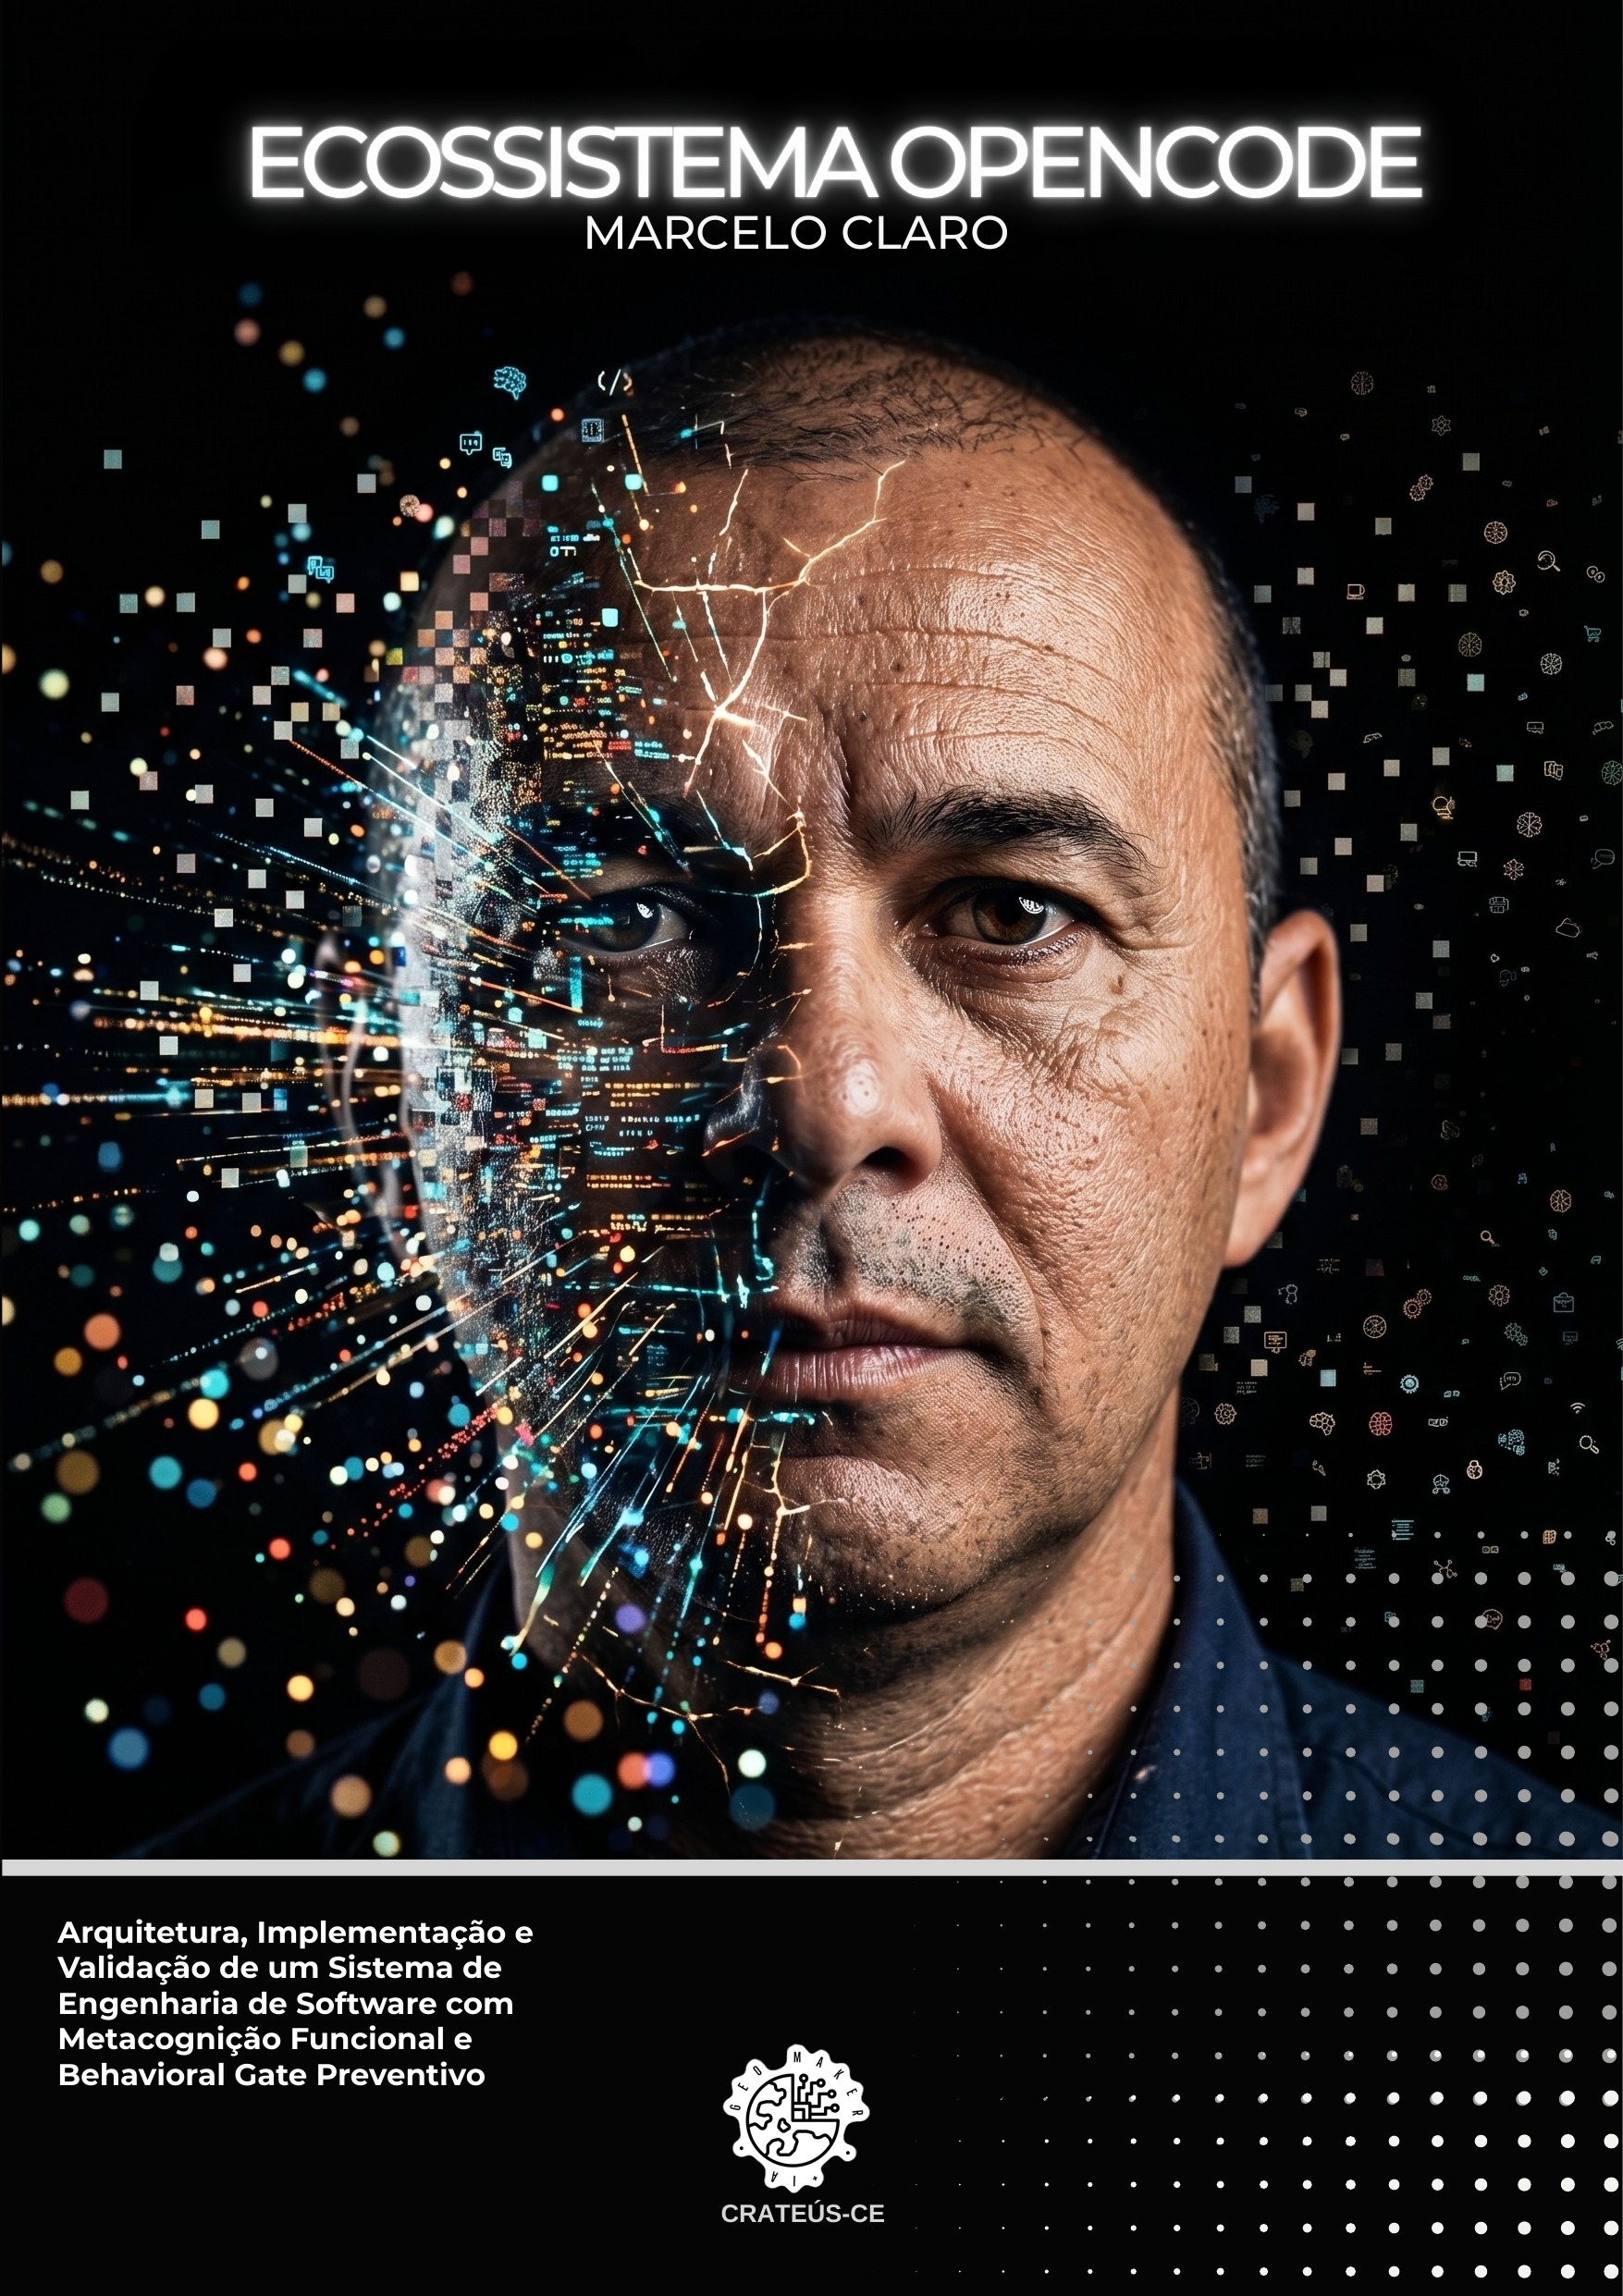
\includegraphics[width=\paperwidth,height=\paperheight]{capa-ecosistema.jpg}};
\end{tikzpicture}%
\null
\clearpage
\pagestyle{fancy}

% --- Prefácio (nota do autor) ---------------------------------
% R621: texto "NOTA DO AUTOR PARA ESTE LIVRO" do PDF do autor, verbatim.
% Mantido como prefácio e não como peça editorial do Core: a voz é a do autor.
\begin{flushleft}
 {\small\sffamily\color{plumAccent}\MakeUppercase{OpenCode Ecosystem Core}\par}
\vspace{2mm}
 {\Large\sffamily\bfseries\color{textmain}Prefácio --- Nota do autor para este livro\par}
{\color{plumAccent}\rule{0.25\linewidth}{1.2pt}\par}
\end{flushleft}
\vspace{2mm}
\begin{elemento}{Nota do autor}{\metainfo{ID}{PREF-01} \hfill \metainfo{Fonte}{arte final do autor} \hfill \metainfo{Ciclo}{R621}}
Este livro nasceu de uma necessidade: democratizar o conhecimento sobre arquitetura de sistemas multiagente. Não basta saber usar IA --- é preciso entender como ela pensa. O ECOSSISTEMA OpenCode é resultado de anos de pesquisa, experimentos e, principalmente, da convicção de que qualquer educador pode construir suas próprias ferramentas.

Dedico este trabalho a todos os professores que, como eu, acreditam que a tecnologia deve servir para ampliar --- nunca substituir --- o potencial humano de criar, questionar e transformar.

Obrigado por fazer parte desta jornada.
\begin{flushright}
--- Marcelo Claro Laranjeira.\\ Crateús, Ceará, 2026.
\end{flushright}
\end{elemento}
\clearpage

% --- Folha de rosto ------------------------------------------
\thispagestyle{plain}
\vspace*{0.20\paperheight}
\begin{center}
\sffamily
{\color{plumAccent}\rule{0.16\linewidth}{1.4pt}}\\[8pt]
{\small\bfseries\color{steel}\MakeUppercase{Série técnica e científica}}\\[12pt]
{\fontsize{25}{29}\selectfont\bfseries\color{textmain}Manual Técnico-Dev-Científico\\[3pt]do OpenCode Ecosystem Core}\\[10pt]
{\color{plumAccent}\rule{0.32\linewidth}{0.8pt}}\\[12pt]
{\large\color{textmuted}Elemento, agente e subagente: ficha de raio-x com descrição, conceito, cálculo,\\
fluxo de trabalho, interações, impacto, limites, arquitetura e fluxograma}\\[22pt]
\begin{tcolorbox}[width=0.9\linewidth,colback=panel,colframe=plumAccent,boxrule=0.6pt,arc=1.5mm,left=5mm,right=5mm,top=4mm,bottom=4mm]
{\small Coordenação do ecossistema: \textbf{MarceloClaro Orchestrator} (proto-coordenação A2A/MetaBus)\\[3pt]
Autor/organizador: \textbf{Marcelo Claro Laranjeira} \;$\cdot$\; ORCID \href{https://orcid.org/0000-0001-8996-2887}{0000-0001-8996-2887} \;$\cdot$\; \texttt{marceloclaro@gmail.com}\\[3pt]
Rigor: protocolos SDD/TDD + política anti-overclaim (CORRIGENDUM)\\[3pt]
Ferramenta de geração: LaTeX (pdf\TeX)}
\end{tcolorbox}
\vspace{14pt}
{\small\itshape\color{textmuted}Livro documental elaborado a partir da leitura do código-fonte, catálogos, especificações,\\
registros de evolução, testes e mapa do ecossistema (MAPA\_ECOSSISTEMA\_COMPLETO).}
\end{center}
\vfill
{\small\sffamily\centering Nenhuma afirmação deste manual deve ser lida como mérito de qualidade externa\\[1pt]
(Qualis A1, benchmark, "superhuman") sem validação externa explícita — ver CORRIGENDUM.\par}
\clearpage

% --- Sumário -------------------------------------------------
\tableofcontents
\clearpage

% ============================================================
%  MODULO 00A — Prologo didatico: A Casa, os Viajantes e o Mapa
%  SPEC R679 — enredo leigo-tecnico, quadriparticao F-S-T-R
%  Citacoes com DOI ativo verificadas em 05/10/2026 via doi.org
% ============================================================
\chapter{Pr\'ologo Did\'atico: A Casa, os Viajantes e o Mapa}

\roteirodidatico
{Imagine uma casa onde moram muitos ajudantes: cada um sabe fazer uma coisa bem feita, mas ningu\'em sozinho d\'a conta de um pedido inteiro. Este pr\'ologo conta como Ana e Bruno entram nessa casa e aprendem a pedir, a conferir e a reconstruir.}
{\emph{Funcional} diz o que a casa entrega vista de fora; \emph{estrutural} mostra quem mora onde e quem chama quem; \emph{te\'orica} explica por que esse jeito de organizar pode funcionar; \emph{reprodu\c{c}\~ao} ensina a refazer o caminho e a conferir cada passo.}
{Acompanhe primeiro a hist\'oria; depois localize cada cena no c\'odigo indicado; por fim refa\c{c}a a verifica\c{c}\~ao proposta e anote o que n\~ao se pode concluir.}
{A casa existe no reposit\'orio; o mapa did\'atico organiza a leitura; a efic\'acia de cada ajudante s\'o se avalia com teste e valida\c{c}\~ao externa. N\'umero de c\^omodos n\~ao prova qualidade do servi\c{c}o.}
{Que cena deste pr\'ologo corresponde a que arquivo do Core, e que evid\^encia observ\'avel distingue inten\c{c}\~ao declarada de comportamento demonstrado?}

\casoguiado{a primeira visita de Ana e Bruno}
{Ana \'e professora em Crate\'us e quer um resumo fiel de um artigo para a aula. Bruno \'e desenvolvedor e quer automatizar a mesma tarefa com rastreio. O narrador, o Orquestrador MarceloClaro, recebe os dois na porta e prop\~oe a mesma regra para ambos: todo pedido entra por um s\'o balc\~ao, \'e dividido em tarefas, \'e encaminhado a quem declara capacidade, e s\'o sai como resposta depois de passar por um crit\'erio escrito. Ana aprende a desconfiar de resposta sem fonte; Bruno aprende a desconfiar de n\'umero sem comando que o recalcule.}

\section{A casa vista da rua: leitura funcional}

Ana n\~ao precisa saber programar para usar a casa. Ela entrega um pedido em portugu\^es, por exemplo resumir um texto, e recebe de volta um texto mais curto com as fontes indicadas. Se faltar a fonte, ela aprende neste livro a devolver a resposta e a pedir de novo. Essa exig\^encia simples, que parece apenas educa\c{c}\~ao, \'e na verdade o primeiro gate de qualidade do Core: sem crit\'erio escrito antes, n\~ao h\'a como aceitar depois.

Bruno v\^e a mesma cena e pergunta o que h\'a por tr\'as do balc\~ao. O narrador responde com quatro palavras que organizam o livro inteiro: funcional, estrutural, te\'orica e reprodu\c{c}\~ao. A leitura funcional responde o que entra e o que sai. Ela n\~ao explica quem fez nem por que deu certo; apenas fixa o contrato. Todo cap\'itulo deste livro come\c{c}a aqui para que o leitor leigo nunca se perca, mesmo quando o detalhe t\'ecnico avan\c{c}a.

A op\c{c}\~ao por come\c{c}ar pelo exemplo resolvido antes do formalismo n\~ao \'e improviso pedag\'ogico. A pesquisa sobre carga cognitiva mostra que resolver buscando fins com an\'alise de meios e fins consome capacidade que faria falta para formar esquemas, e que exemplos trabalhados reduzem essa busca.

Essa orienta\c{c}\~ao did\'atica justifica o enredo deste livro: cada conceito aparece primeiro numa cena concreta de Ana e Bruno, depois em vocabul\'ario preciso, depois no mecanismo e s\'o ent\~ao na formaliza\c{c}\~ao \citref{SWELLER, J. Cognitive load during problem solving: effects on learning. Cognitive Science, v.~12, n.~2, p.~257-285, 1988}{10.1016/0364-0213(88)90023-7}{Justifica o metodo didatico deste livro: comecar por exemplo guiado e so entao formalizar, para nao sobrecarregar a memoria de trabalho do leitor iniciante.}{Considerable evidence indicates that domain specific knowledge in the form of schemas is the primary factor distinguishing experts from novices in problem-solving skill}{Ha evidencia consideravel de que o conhecimento especifico de dominio, na forma de esquemas, e o principal fator que distingue especialistas de novatos na habilidade de resolver problemas.}{SWELLER, 1988, p.~257-285}.

\section{Quem mora onde: primeira leitura estrutural}

Quando Ana entra, o narrador apresenta os moradores sem jarg\~ao. H\'a o Orquestrador, que atende no balc\~ao e nunca deixa dois balc\~oes atenderem ao mesmo tempo. H\'a os Agentes, cada um com uma plaquinha dizendo o que sabe tentar. H\'a o Quadro Negro, uma lousa onde o Orquestrador anota quem ficou com cada parte. H\'a a Mem\'oria, um caderno onde ficam guardados o que j\'a foi tentado e o que se aprendeu. H\'a as Especifica\c{c}\~oes e os Testes, dois fiscais que s\'o carimbam a sa\'ida se o prometido foi cumprido.

Bruno traduz cada morador para um caminho de arquivo. O Orquestrador mora em \pth{marceloclaro/orchestrator.py}. Os Agentes est\~ao declarados em \pth{opencode.json} e descritos em \pth{agents/catalog/}. O Quadro Negro \'e o protocolo Blackboard A2A. A Mem\'oria \'e o MetaBus em \pth{mci/}. Os fiscais s\~ao \pth{specs/SPEC-935-R*.md} e \pth{tests/test_r*.py}. Essa tradu\c{c}\~ao \'e a leitura estrutural: ela liga cada personagem a um lugar observ\'avel no reposit\'orio, para que nenhuma afirma\c{c}\~ao do livro dependa apenas da hist\'oria.

A ideia de dividir uma tarefa entre especialistas que se comunicam por uma lousa comum tem origem documentada na literatura de sistemas blackboard, onde fontes de conhecimento independentes cooperam pela estrutura do quadro.

O vocabul\'ario quadro e fonte de conhecimento usado neste livro vem dessa tradi\c{c}\~ao, e \'e ele que permite distinguir o canal de comunica\c{c}\~ao do conte\'udo que por ele trafega \citref{NII, H. P. Blackboard systems: the blackboard model of problem solving and the evolution of blackboard architectures. AI Magazine, v.~7, n.~2, p.~38-53, 1986}{10.1609/aimag.v7i2.537}{Da proveniencia ao Quadro Negro A2A do Core: fontes de conhecimento independentes que cooperam por um quadro compartilhado.}{The first blackboard system was the HEARSAY-II speech understanding system that evolved between 1971 and 1976}{O primeiro sistema blackboard foi o sistema de compreensao de fala HEARSAY-II, que evoluiu entre 1971 e 1976.}{NII, 1986, p.~38-53}.

Para que Ana n\~ao confunda ajudante com m\'agica, o livro fixa desde j\'a a defini\c{c}\~ao de agente que atravessa todos os cap\'itulos: componente reativo, proativo e social, cuja ativa\c{c}\~ao s\'o conta quando h\'a gatilho registrado, regra de roteamento e entrega confrontada com crit\'erio.

Essa tr\'iade reatividade, proatividade e habilidade social \'e o lastro que separa um script de um agente, e ser\'a retomada em cada ficha do cat\'alogo \citref{WOOLDRIDGE, M.; JENNINGS, N. R. Intelligent agents: theory and practice. The Knowledge Engineering Review, v.~10, n.~2, p.~115-152, 1995}{10.1017/S0269888900008122}{Fundamenta quando um gatilho e de fato ativacao de agente neste livro: reatividade, proatividade e habilidade social convertidas em regras de roteamento.}{The concept of an agent has become important in both artificial intelligence and mainstream computer science}{O conceito de agente tornou-se importante tanto na inteligencia artificial quanto na ciencia da computacao.}{WOOLDRIDGE; JENNINGS, 1995, p.~115-152}.

\elemento{A Casa e seus moradores}{\metainfo{ID}{ENR-00A} \hfill \metainfo{Leitura}{funcional + estrutural} \hfill \metainfo{Rota}{AGENTS.md, opencode.json, mci/}}

\begin{descricao}
Ana usa a casa sem abrir o cap\^o: entrega pedido, recebe resposta com fonte, devolve sem fonte. Bruno abre o cap\^o: confere \pth{opencode.json} para contar agentes, abre \pth{marceloclaro/orchestrator.py} para ver o balc\~ao \'unico, abre \pth{mci/} para ver a mem\'oria. Os dois fazem a mesma pergunta por caminhos distintos: que evid\^encia sustenta esta resposta. O livro nunca permite que a hist\'oria substitua o arquivo.
\end{descricao}

\begin{funcao}
Fixar o contrato did\'atico: todo cap\'itulo ter\'a cena, vocabul\'ario, mecanismo, evid\^encia e limite. O leigo pode parar na cena e no vocabul\'ario; o t\'ecnico deve seguir at\'e o arquivo e o comando.
\end{funcao}

\section{A f\'isica da casa: primeira leitura te\'orica}

Na terceira noite, Ana pergunta por que anotar tanto. O narrador responde que gente esquece e tamb\'em se engana com confian\c{c}a. Por isso a casa mant\'em um caderno de metacogni\c{c}\~ao: n\~ao apenas o que foi feito, mas o que se pensou sobre o que foi feito. Essa distin\c{c}\~ao entre fazer e monitorar o fazer \'e antiga na psicologia do desenvolvimento e d\'a nome ao MetaBus do Core.

A literatura fundadora descreve o monitoramento cognitivo como o conhecimento que a pessoa tem sobre seus pr\'oprios processos, e \'e essa defini\c{c}\~ao que este livro usa quando fala em mem\'oria metacognitiva persistida.

Sem esse caderno, cada pedido come\c{c}aria do zero; com ele, o erro de ontem vira crit\'erio de amanh\~a \citref{FLAVELL, J. H. Metacognition and cognitive monitoring: a new area of cognitive-developmental inquiry. American Psychologist, v.~34, n.~10, p.~906-911, 1979}{10.1037/0003-066X.34.10.906}{Sustenta o MetaBus como memoria metacognitiva: conhecimento e monitoramento sobre os proprios processos, nao apenas log de eventos.}{Cognitive monitoring refers to the knowledge one has about one's own cognitive processes}{Monitoramento cognitivo refere-se ao conhecimento que se tem sobre os proprios processos cognitivos.}{FLAVELL, 1979, p.~906-911}.

Bruno pergunta ent\~ao por que tanta desconfian\c{c}a com n\'umeros bonitos. O narrador mostra o c\'alculo que ser\'a repetido no pr\'oximo cap\'itulo como vacina quantitativa. Suponha $N$ sa\'idas reunidas, cada uma correta com probabilidade $p$, com erros independentes. A probabilidade de todas estarem corretas \'e $p^{N}$. Logo a probabilidade de ao menos um erro \'e o complementar.

\[ P(\mbox{ao menos um erro}) = 1 - p^{N}. \]

Com $N=216$ e $p=0{,}99$, tem-se $\ln(0{,}99^{216}) = 216 \ln 0{,}99 \approx -2{,}17$, logo $0{,}99^{216} \approx 0{,}114$ e $P \approx 0{,}886$, cerca de 89 por cento. O n\'umero 216 ilustra a f\'ormula com o tamanho do cat\'alogo; n\~ao afirma que o Core agregue 216 respostas nem mede sua taxa de erro. A li\c{c}\~ao te\'orica \'e geral: agregar muitas sa\'idas sem gate cobra pre\c{c}o probabil\'istico, e gate com crit\'erio expl\'icito existe para tornar esse pre\c{c}o inspecion\'avel.

\section{A planta para reconstruir: leitura de reprodu\c{c}\~ao}

Na \'ultima cena do pr\'ologo, Ana e Bruno ganham a mesma planta. Ela tem doze passos, do clone ao PDF recompilado, cada um com comando, sa\'ida esperada e modo de conferir. A planta ser\'a executada no ep\'ilogo, mas seu princ\'ipio j\'a aparece aqui: pesquisa s\'o \'e ci\^encia quando outro consegue refazer o caminho com os mesmos materiais e comparar o resultado.

Essa exig\^encia de transpar\'encia do fluxo, dos dados e do ambiente \'e o cora\c{c}\~ao da ci\^encia computacional reproduz\'ivel, e \'e ela que justifica que este livro trate comandos, vers\~oes e seeds como parte do texto, n\~ao como anexo.

Reproduzir n\~ao \'e repetir por repetir: \'e permitir que o leitor troque uma pe\c{c}a e observe o efeito, mantendo o restante fixo \citref{PENG, R. D. Reproducible research in computational science. Science, v.~334, n.~6060, p.~1226-1227, 2011}{10.1126/science.1213847}{Justifica tratar ambiente, codigo e dados como parte do relato cientifico e exigir planta de reproducao executavel neste livro.}{Reproducible research is the idea that the ultimate product of academic research is the paper along with the full computational environment}{Pesquisa reproduzivel e a ideia de que o produto final da pesquisa academica e o artigo junto com o ambiente computacional completo.}{PENG, 2011, p.~1226-1227}.

\begin{aviso}
Limite do pr\'ologo. A hist\'oria de Ana e Bruno \'e recurso did\'atico para ordenar a leitura; n\~ao constitui evid\^encia de efic\'acia de nenhum agente. Contagens citadas s\~ao fotografias do checkout e devem ser recalculadas. Tradu\c{c}\~oes de trechos s\~ao livres e n\~ao substituem o original.
\end{aviso}

% ============================================================
%  MODULO 00B — Jornada do Leitor: do Funcional ao Reprodutivel
%  SPEC R679 — quatro estacoes F-S-T-R com calculos justificados
% ============================================================
\chapter{Jornada do Leitor: Quatro Esta\c{c}\~oes}

\roteirodidatico
{Voc\^e pode ler este livro em dois ritmos: Ana l\^e para usar bem; Bruno l\^e para reconstruir. As quatro esta\c{c}\~oes a seguir mostram o mesmo pedido visto de quatro dist\^ancias: o que a casa promete, quem executa, por que o desenho faz sentido e como refazer.}
{\emph{Esta\c{c}\~ao Funcional} observa entradas e sa\'idas; \emph{Estrutural} abre o cap\^o e localiza arquivos; \emph{Te\'orica} apresenta o modelo que justifica a regra; \emph{Reprodu\c{c}\~ao} fixa comando, vers\~ao e confer\^encia.}
{Em cada esta\c{c}\~ao, pare na pergunta de verifica\c{c}\~ao antes de avan\c{c}ar. Se n\~ao conseguir responder com arquivo ou comando, volte uma esta\c{c}\~ao.}
{Modelos inspiram regras; regras n\~ao provam desempenho. DOI ativo prova localiza\c{c}\~ao da fonte, n\~ao acerto da interpreta\c{c}\~ao. C\'alculos valem dentro das hip\'oteses declaradas.}
{Para o pedido que voc\^e tem em mente, o que muda entre ver s\'o a resposta e conseguir refazer todo o caminho com outro computador?}

\casoguiado{o pedido que atravessa as quatro esta\c{c}\~oes}
{Ana pede: resuma este artigo em dez linhas sem inventar dados. Bruno registra o mesmo pedido como tarefa com crit\'erio: cada frase do resumo deve apontar para um trecho do original. Na esta\c{c}\~ao funcional, ambos conferem se o resumo veio com fontes. Na estrutural, Bruno localiza quem buscou, quem resumiu e quem verificou. Na te\'orica, os dois entendem por que gates existem. Na reprodu\c{c}\~ao, Bruno repete o diagn\'ostico e recompila o livro para provar que o ambiente sustenta o que o texto afirma.}

\section{Esta\c{c}\~ao Funcional: o contrato antes do mecanismo}

Na esta\c{c}\~ao funcional, a \'unica pergunta \'e se o combinado foi cumprido. Entrada, crit\'erio e sa\'ida ficam vis\'iveis na mesma p\'agina. Ana aprende a exigir tr\^es itens: o texto pedido, a fonte de cada afirma\c{c}\~ao e a declara\c{c}\~ao do que n\~ao foi encontrado. Sem esses tr\^es, ela devolve. Bruno aprende a escrever o crit\'erio antes de chamar qualquer agente, em \pth{specs/SPEC-935-R*.md}, e a s\'o aceitar a entrega quando \pth{tests/test_r*.py} passa. Essa ordem, crit\'erio antes de execu\c{c}\~ao, \'e o SDD/TDD que o livro defender\'a com dados.

A defesa n\~ao \'e slogan \'agil. A disseca\c{c}\~ao do processo mostra que os ganhos associados ao TDD v\^em sobretudo da granularidade e da uniformidade dos passos, n\~ao apenas da ordem teste-primeiro.

Passos curtos e regulares melhoram foco e fluxo, e \'e por isso que este livro exige fichas curtas, comandos curtos e verifica\c{c}\~oes frequentes em vez de grandes blocos sem confer\^encia \citref{FUCCI, D. et al. A dissection of the test-driven development process: does it really matter to test-first or to test-last? IEEE Transactions on Software Engineering, v.~43, n.~7, p.~597-614, 2017}{10.1109/TSE.2016.2616877}{Justifica o SDD/TDD deste livro como disciplina de passos curtos e uniformes, nao como ritual de ordem teste-primeiro.}{Test-driven development is a technique that repeats short coding cycles interleaved with testing}{Desenvolvimento orientado a testes e uma tecnica que repete ciclos curtos de codificacao intercalados com testes.}{FUCCI et al., 2017, p.~597-614}.

A meta-an\'alise de 27 estudos sobre TDD confirma o mesmo ponto com outra lente: h\'a efeito sobre qualidade externa e produtividade, mas condicionado ao desenho do estudo e \`a granularidade da pr\'atica.

Por isso o livro nunca promete que spec mais teste eliminam erro; promete apenas que tornam o crit\'erio inspecion\'avel e a falha localiz\'avel \citref{RAFIQUE, Y.; MISIC, V. B. The effects of test-driven development on external quality and productivity: a meta-analysis. IEEE Transactions on Software Engineering, v.~39, n.~6, p.~835-856, 2013}{10.1109/TSE.2012.28}{Delimita o que o SDD/TDD pode prometer neste livro: efeito condicionado e auditavel, nao garantia universal de qualidade.}{This paper provides a systematic meta-analysis of 27 studies that investigate the impact of test-driven development on external code quality}{Este artigo fornece uma meta-analise sistematica de 27 estudos que investigam o impacto do desenvolvimento orientado a testes na qualidade externa do codigo.}{RAFIQUE; MISIC, 2013, p.~835-856}.

\elemento{Contrato funcional m\'inimo}{\metainfo{ID}{JOR-F} \hfill \metainfo{Para}{Ana e Bruno} \hfill \metainfo{Gate}{fail-closed}}

\begin{descricao}
Todo pedido traz entrada leg\'ivel, crit\'erio escrito e forma de conferir. Se faltar um dos tr\^es, o Orquestrador recusa encerrar. Essa recusa n\~ao \'e antipatia: \'e o gate fechado que protege o leitor de aceitar resposta sem lastro.
\end{descricao}

\section{Esta\c{c}\~ao Estrutural: quem faz e onde mora}

Na esta\c{c}\~ao estrutural, Bruno abre o mapa de oito camadas e segue o pedido como quem segue um cano. Camada 1 recebe pela CLI e configura\c{c}\~ao. Camada 3 escolhe o agente por capacidades e escore. Camada 2 anota no Quadro e guarda no MetaBus. Camada 4 barra o que n\~ao passou no gate. Camada 6 chama ferramentas externas por MCP quando precisa. Cada passagem deixa rastro em arquivo ou log; onde n\~ao h\'a rastro, n\~ao h\'a afirma\c{c}\~ao neste livro.

O cora\c{c}\~ao da escolha \'e uma pontua\c{c}\~ao de aten\c{c}\~ao. Por tr\'as do nome elegante h\'a uma opera\c{c}\~ao simples herdada dos Transformers: comparar pergunta e candidatos por produto escalar, suavizar por softmax e combinar valores.

A arquitetura que introduziu esse mecanismo empilha aten\c{c}\~ao pura sem recorr\^encia nem convolu\c{c}\~ao, e \'e dela que o Core toma emprestada a ideia de rotear por relev\^ancia ponderada.

O mecanismo original calcula aten\c{c}\~ao como softmax do produto de consultas por chaves escalado pela raiz da dimens\~ao, ponderando valores \citref{VASWANI, A. et al. Attention is all you need. Advances in Neural Information Processing Systems, v.~30, p.~5998-6008, 2017}{10.48550/arXiv.1706.03762}{Justifica o roteamento por atencao do Core como ponderacao por relevancia, nao como compreensao garantida.}{We propose a new simple network architecture, the Transformer, based solely on attention mechanisms, dispensing with recurrence and convolutions entirely}{Propomos uma nova arquitetura de rede simples, o Transformer, baseada apenas em mecanismos de atencao, dispensando totalmente recorrencia e convolucoes.}{VASWANI et al., 2017, p.~5998-6008}.

Para que Ana tamb\'em entenda, o livro resolve um caso de brinquedo. Sejam duas consultas e duas chaves em dimens\~ao $d_{k}=4$, com $QK^{T} = [[4,0],[0,4]]$. Escala por $\sqrt{d_{k}}=2$: $[[2,0],[0,2]]$. Softmax por linha: linha 1 d\'a $[\exp(2)/(\exp(2)+\exp(0)), 1/(\exp(2)+1)] \approx [0{,}88, 0{,}12]$; linha 2 espelha $[0{,}12, 0{,}88]$. Multiplicar por $V=[[1,0],[0,1]]$ devolve quase a identidade ponderada. O exemplo mostra o essencial: escore alto concentra peso, escore empatado divide peso. No Core, trocar $Q$, $K$ e $V$ por embeddings de tarefa, agente e hist\'orico n\~ao muda a intui\c{c}\~ao: pontua\c{c}\~ao ordena, n\~ao certifica.

\begin{aviso}
Limite estrutural. O c\'alculo acima ilustra pondera\c{c}\~ao; n\~ao prova que o roteador do Core escolha bem. A qualidade da escolha depende de embeddings, pesos, desempates e fallbacks implementados, avaliados caso a caso com registros observ\'aveis.
\end{aviso}

\section{Esta\c{c}\~ao Te\'orica: por que desconfiar at\'e com n\'umero bonito}

Na esta\c{c}\~ao te\'orica, Ana aprende a pergunta que protege o leigo: de cada dez afirma\c{c}\~oes publicadas nesta \'area, quantas seriam verdadeiras antes deste estudo. Bruno aprende a f\'ormula que formaliza a desconfian\c{c}a: o valor preditivo positivo.

O ensaio que fundou essa discuss\~ao mostra que a probabilidade de uma alega\c{c}\~ao ser verdadeira depende de poder, vi\'es e da raz\~ao entre rela\c{c}\~oes verdadeiras e falsas testadas no campo.

Simula\c{c}\~oes desse modelo indicam que, para muitos desenhos e campos, \'e mais prov\'avel que uma alega\c{c}\~ao seja falsa do que verdadeira, o que justifica o gate anti-overclaim deste livro \citref{IOANNIDIS, J. P. A. Why most published research findings are false. PLoS Medicine, v.~2, n.~8, e124, 2005}{10.1371/journal.pmed.0020124}{Fundamenta o gate anti-overclaim e o calculo de PPV: sem considerar poder, vies e razao de verdadeiros, numero bonito nao sustenta conclusao.}{Simulations show that for most study designs and settings, it is more likely for a research claim to be false than true}{Simulacoes mostram que, para a maioria dos desenhos e cenarios de estudo, e mais provavel que uma alegacao de pesquisa seja falsa do que verdadeira.}{IOANNIDIS, 2005, e124}.

O livro resolve o caso can\^onico. Seja $R$ a raz\~ao entre verdadeiros e falsos antes do estudo, $\alpha=0{,}05$ o n\'ivel de signific\^ancia e $1-\beta$ o poder. Ent\~ao

\[ \mathrm{PPV} = \frac{(1-\beta)R}{(1-\beta)R + \alpha}. \]

Com campo dif\'icil $R=1{:}10=0{,}1$, poder $0{,}8$ e $\alpha=0{,}05$: numerador $0{,}8 \times 0{,}1 = 0{,}08$; denominador $0{,}08+0{,}05=0{,}13$; $\mathrm{PPV} \approx 0{,}615$, cerca de 62 por cento. Ou seja, mesmo com poder razo\'avel, tr\^es a cada oito achados significativos seriam falsos nesse campo. Se houver vi\'es $u$, o denominador cresce e o PPV cai mais. A moral para o Core \'e direta: teste verde sem considerar poder, vi\'es e taxa-base n\~ao \'e selo de verdade; \'e apenas passagem por um crit\'erio declarado.

\section{Esta\c{c}\~ao Reprodu\c{c}\~ao: como refazer sem depender de ningu\'em}

Na \'ultima esta\c{c}\~ao, Bruno executa e Ana confere. O princ\'ipio que organiza a planta de doze passos do ep\'ilogo vem dos princ\'ipios FAIR: para que m\'aquinas e pessoas encontrem, acessem, combinem e reutilizem, dados e metadados precisam de identificador persistente, descri\c{c}\~ao rica e registro indexado.

A urg\^encia de melhorar a infraestrutura de reutiliza\c{c}\~ao \'e o diagn\'ostico que motiva tratar specs, testes, logs e vers\~oes como cidad\~aos de primeira classe neste livro.

Cada artefato do Core ganha, por isso, proveni\^encia: quem gerou, de que vers\~ao, com que comando e com que hash \citref{WILKINSON, M. D. et al. The FAIR Guiding Principles for scientific data management and stewardship. Scientific Data, v.~3, 160018, 2016}{10.1038/sdata.2016.18}{Justifica a planta de reproducao e a proveniencia por observacao exigidas neste livro: tornar cada entrega encontrravel, acessivel e reutilizavel.}{There is an urgent need to improve the infrastructure supporting the reuse of scholarly data}{Ha uma necessidade urgente de melhorar a infraestrutura que sustenta a reutilizacao de dados academicos.}{WILKINSON et al., 2016, 160018}.

\elemento{As quatro esta\c{c}\~oes em uma frase}{\metainfo{ID}{JOR-SINT} \hfill \metainfo{Uso}{guia de bolso}}

\begin{descricao}
Funcional promete o contrato; estrutural mostra o encanamento; te\'orica explica o porqu\^e do gate; reprodu\c{c}\~ao entrega a chave para refazer. Se voc\^e consegue contar a mesma cena nas quatro linguagens, entendeu o Core o bastante para us\'a-lo sem se enganar.
\end{descricao}

\begin{funcao}
Dar ao leigo um caminho seguro at\'e o uso com fontes e ao t\'ecnico um caminho audit\'avel at\'e a reconstru\c{c}\~ao, sem que um precise fingir ser o outro.
\end{funcao}

% ============================================================
%  MODULO 18 — Nivel 0 Universal: todos os termos para leigos
%  SPEC R682 — camada tradutora, sem reescrever 378 fichas
% ============================================================
\chapter{N\'ivel 0 Universal: O Dicion\'ario da Casa}

\roteirodidatico
{Se alguma palavra deste livro travou sua leitura, venha para ca. Este capitulo traduz todos os termos dificeis para a linguagem da casa, com uma frase curta, uma comparacao e o lugar onde o tecnico confere.}
{\emph{N\'ivel 0} e entender o bastante para usar sem se enganar; \emph{termo discriminado} e palavra com sentido proprio neste livro; \emph{familia} e grupo de agentes com trabalho parecido.}
{Ache a palavra na lista, leia a frase, guarde a comparacao e, se quiser ir alem, abra o caminho indicado.}
{Traducao ajuda a usar; so arquivo e comando provam. Analogia nao e definicao tecnica.}
{Que palavra travou voce, e o que voce consegue fazer com ela depois da traducao?}

\casoguiado{Dona Ana usa o dicionario}
{Ana le gate fail-closed e trava. Vem aqui, acha Gate: fiscal que devolve sem nota. Lembra da prova com gabarito. Volta ao texto e entende: sem nota, volta. Levou vinte segundos e nao precisou programar.}

\section{Ler qualquer ficha em um minuto}

\begin{flowch}[Qualquer ficha em 5 olhares]{fonte: metodo META-LEITURA do mod-01}
\matrix[matrix of nodes,name=n0,row sep=2.2mm,column sep=2.5mm,nodes={fn},ampersand replacement=\&]{
 |[fns]|1 Frase: o que promete \\
 |[fn]|2 Comparacao: com o que parece \\
 |[fn]|3 Rastro: onde se confere \\
 |[fde]|4 Passou no criterio \\
 |[fne]|5 Uso com limite \\
};
\draw[seta] (n0-1-1.south)--(n0-2-1.north);
\draw[seta] (n0-2-1.south)--(n0-3-1.north);
\draw[seta] (n0-3-1.south)--(n0-4-1.north);
\draw[seta] (n0-4-1.south)--(n0-5-1.north);
\end{flowch}

\begin{descricao}
Um minuto por ficha: leia a promessa, fixe a comparacao, localize o rastro em arquivo ou comando, pergunte se passou no criterio e anote o limite. Se faltar rastro, pare: sem rastro nao ha conclusao, so conversa.
\end{descricao}

\begin{flowch}[Termo dificil vira uso seguro]{fonte: glossario abaixo}
\matrix[matrix of nodes,name=n0b,row sep=3mm,column sep=4mm,nodes={fn},ampersand replacement=\&]{
 |[fn]|Palavra nova \& |[fn]|Frase de 12 palavras \\
 |[fn]|Comparacao da casa \& |[fne]|Conferencia no codigo \\
};
\draw[seta] (n0b-1-1)--(n0b-1-2);
\draw[seta] (n0b-1-2.south)--(n0b-2-1.north);
\draw[seta] (n0b-2-1)--(n0b-2-2);
\end{flowch}

\section{Glossario A a Z em linguagem da casa}

\elemento{Dicionario nivel 0: como usar}{\metainfo{ID}{N0-DIC} \hfill \metainfo{Regra}{frase mais comparacao mais morada}}

\begin{descricao}
Cada item tem frase curta, comparacao com a casa e, quando existe, a morada no codigo entre parenteses. Morada serve ao tecnico; frase e comparacao bastam ao leigo.
\end{descricao}

\begin{descricao}
\textbf{Agente:} ajudante com plaquinha do que tenta. Como plantonista com especialidade do dia. Mora em \pth{agents/catalog/}. \textbf{Orquestrador:} porteiro unico que distribui sem fazer o servico. Como sindico que escala. Mora em \pth{marceloclaro/orchestrator.py}. \textbf{Blackboard:} lousa onde todos veem quem faz o que. Como quadro de plantao. \textbf{MetaBus:} caderno de licoes aprendidas. Como livro de ocorrencias. Mora em \pth{mci/}. \textbf{Memoria episodica:} o que aconteceu. Como diario. \textbf{Memoria semantica:} licao tirada. Como regra da casa. \textbf{Spec:} combinado escrito antes. Como receita. Mora em \pth{specs/}. \textbf{Teste:} prova com gabarito. Como simulado. Mora em \pth{tests/}. \textbf{Gate:} fiscal que devolve sem nota. Como porteira de prova. \textbf{Fail-closed:} na duvida, reprova. Como porteira que nao abre sem cracha. \textbf{SDD:} nada sem combinado. Como obra sem projeto nao comeca. \textbf{TDD:} ciclo curto com teste. Como provar roupa a cada ajuste. \textbf{Escore:} nota de parecido. Como formato da chave. \textbf{Jaccard:} parecido sobre total. Como pecas iguais sobre pecas vistas. \textbf{Atencao:} peso para o parecido. Como ouvir mais quem sabe do assunto. \textbf{Roteamento:} escolher destino. Como mesa que encaminha guia. \textbf{Delegacao:} passar com dono anotado. Como escala assinada. \textbf{Voluntariado:} quem pode se oferece. Como plantao que aceita caso. \textbf{CFP:} anuncio de vaga. Como edital na lousa. \textbf{Lease:} posse temporaria. Como turno com horario. \textbf{Fallback:} plano B. Como estepe. \textbf{Carga:} ocupacao. Como fila de espera. \textbf{Confianca:} pontos de quem acerta. Como credito na cantina, interno e nao garantia. \textbf{Proveniencia:} quem fez, quando, com o que. Como nota fiscal. \textbf{Hash:} digital do arquivo. Como impressao digital. \textbf{Seed:} numero que fixa sorteio. Como senha do bingo. \textbf{Versao:} foto datada. Como edicao do jornal. \textbf{Commit:} ponto salvo. Como capitulo gravado. \textbf{CLI:} janela de comandos. Como balcao de digitacao. \textbf{MCP:} tomada padrao para ferramenta. Como tomada universal. \textbf{A2A:} conversa entre ajudantes. Como radio da equipe. \textbf{Skill:} receita pronta. Como modo de preparo. \textbf{Catalogo:} lista de ajudantes. Como lista de ramais. Mora em \pth{opencode.json}. \textbf{Executor externo:} vizinho que ajuda. Como Gemini e Reasonix chamados quando precisa. \textbf{Reversa:} engenharia de mapa antigo. Como reforma com planta velha. \textbf{Transformer:} maquina de dar peso. Como balanca de parecido. \textbf{Embedding:} numero que resume sentido. Como apelido numerico. \textbf{Softmax:} reparte cem por cento. Como dividir pizza por fome. \textbf{Poder:} chance de achar o que existe. Como faro bom. \textbf{Alfa:} tolerancia a alarme falso. Como cinco em cem. \textbf{PPV:} de cada achado, quanto presta. Como peixe bom na rede. \textbf{Vies:} torta na balanca. Como vento a favor de um lado. \textbf{Taxa-base:} quanto ja era comum. Como peixe que ja tinha no lago. \textbf{FAIR:} facil de achar, abrir, juntar e reusar. Como biblioteca arrumada. \textbf{Reproducao:} refazer e comparar. Como repetir receita. \textbf{Fotografia:} contagem datada. Como censo do predio. \textbf{Doctor:} check-up da casa. Como comando \pth{python3 -m marceloclaro.cli doctor}. \textbf{Ciclo de evolucao:} aprendizado gravado. Como ata numerada R47 em diante. \textbf{Corrigendum:} lista de exageros corrigidos. Como errata na porta. \textbf{Anti-overclaim:} sem selo sem prova externa. Como sem diploma sem escola. \textbf{Metacognicao:} pensar sobre o pensar. Como revisar a propria prova. \textbf{Reflexao:} resumo do que houve. Como relatorio de plantao. \textbf{Percebe:} olhar lousa e caderno antes. Como passar visita. \textbf{Delega:} encaminhar com criterio. Como distribuir guias. \textbf{Executa:} fazer com ferramenta. Como cozinhar com ingredientes. \textbf{Reflete:} guardar licao. Como atualizar livro de ocorrencias. \textbf{Camada:} andar da casa. Como do zero ao sete. \textbf{Interface:} porta de entrada. Como recepcao. \textbf{Infra:} luz, agua e chave. Como Ollama e credenciais. \textbf{Seguranca:} fechadura e cofre. Como permissao e segredo. \textbf{Benchmark:} corrida com cronometro. Como comparacao datada, nao titulo. \textbf{Qualis:} selo externo de revista. Como este livro nao da a ninguem sozinho. \textbf{Mind map:} desenho das ideias. Como arvore da materia. \textbf{Infografico:} cartaz que explica. Como painel do corredor. \textbf{NotebookLM:} caderno que responde com fonte. Como biblioteca que cita pagina.
\end{descricao}

\section{Cinco fichas-modelo traduzidas para todos os tipos de caixa}

\elemento{Modelo 1 -- Gate fail-closed}{\metainfo{ID}{N0-M1} \hfill \metainfo{Cobre}{processo mais limite}}

\begin{descricao}
Promessa: nada passa sem criterio. Comparacao: prova com gabarito. Rastro: spec mais teste verde. Limite: gabarito fora do assunto nao aprova nada.
\end{descricao}

\begin{funcao}
Proteger o leigo do quase: sem nota, volta com motivo escrito.
\end{funcao}

\elemento{Modelo 2 -- Blackboard}{\metainfo{ID}{N0-M2} \hfill \metainfo{Cobre}{conceito mais arquitetura}}

\begin{descricao}
Promessa: todos veem quem faz o que. Comparacao: quadro de plantao. Rastro: entradas do Quadro com tarefa e dono. Limite: lousa cheia nao prova servico bom.
\end{descricao}

\begin{funcao}
Evitar duplicar e sumir com dono: sem nome na lousa, ninguem responde.
\end{funcao}

\elemento{Modelo 3 -- Atencao e Jaccard}{\metainfo{ID}{N0-M3} \hfill \metainfo{Cobre}{metodo mais calculo}}

\begin{descricao}
Promessa: ordenar por parecido. Comparacao: chave pelo formato. Conta: parecido sobre total, empate por categoria. Limite: parecido nao e acerto.
\end{descricao}

\begin{funcao}
Escolher sem fingir certeza: nota guia, fiscal decide.
\end{funcao}

\elemento{Modelo 4 -- PPV}{\metainfo{ID}{N0-M4} \hfill \metainfo{Cobre}{resultado mais aviso}}

\begin{descricao}
Promessa: dizer quanto do achado presta. Comparacao: peixe bom na rede. Conta: com campo dificil, 62 em 100 prestam; com campo facil, 94. Limite: mesmo teste vale diferente por campo.
\end{descricao}

\begin{funcao}
Vacinar contra numero bonito: sem taxa-base, sem conclusao.
\end{funcao}

\elemento{Modelo 5 -- FAIR e reproducao}{\metainfo{ID}{N0-M5} \hfill \metainfo{Cobre}{reproducao completa}}

\begin{descricao}
Promessa: outro refaz e compara. Comparacao: receita com ingredientes e forno. Rastro: comando, versao, hash e seed. Limite: outra maquina pode divergir por dependencia externa; guardar saida real e parte do metodo.
\end{descricao}

\begin{funcao}
Transformar leitor em testemunha: sem rastro, e historia; com rastro, e ciencia repetivel.
\end{funcao}

\section{O catalogo inteiro em 14 frases}

\begin{descricao}
Orquestracao: quem distribui sem executar. Academica e pesquisa: quem busca e cita sem inventar. Auditoria: quem confere e aponta furo. Juridica: quem redige com norma. Dados: quem trata com origem e permissao. Inferencia: quem calcula com limite. Engenharia e nuvem: quem liga servico com chave. Testes: quem prova com gabarito. Literaria: quem cria e revisa com etica. Curadoria: quem organiza paisagem. Integracao: quem liga ponta com contrato. Mira e apresentacao: quem mostra em cartaz. Qualidade e MASWOS: quem fecha pacote sem prometer selo. Utilidade: quem ajuda no dia a dia com comando curto. Cada um dos 238 segue a mesma leitura de um minuto da primeira secao.
\end{descricao}

\begin{aviso}
Limite do nivel 0. Frase curta ajuda a comecar; nao substitui spec, teste e gate. Quando a duvida envolve dinheiro, saude, justica ou seguranca, chame responsavel humano e repita a conferencia com criterio escrito.
\end{aviso}

% ============================================================
%  MÓDULO 02 (FRONT) — Fundações: o que é o Core, método e rigor
% ============================================================
\chapter{Visão Geral do Ecossistema}

\roteirodidatico
{Comece pela situação de uma tarefa que precisa de várias etapas: localizar a informação, decidir quem pode tratá-la e verificar a resposta. O Core organiza componentes para coordenar esse percurso.}
{\emph{Agente} é um componente especializado; \emph{orquestrador} organiza tarefas; \emph{ferramenta} executa uma operação; \emph{evidência} é o registro observável que sustenta uma conclusão.}
{Leia primeiro o mapa de responsabilidades; depois acompanhe uma solicitação entre componentes; por fim, compare as alegações do manual com arquivos, configurações e diagnóstico.}
{Separe arquitetura declarada, comportamento implementado, disponibilidade no ambiente e eficácia medida. São níveis de afirmação distintos, e um não prova automaticamente o seguinte.}
{Para uma capacidade descrita neste capítulo, que arquivo demonstra que ela existe, que comando demonstra que está disponível e que avaliação demonstraria que produz bons resultados?}

\casoguiado{uma tarefa de resumo}
{Suponha que alguém peça um resumo de um artigo. O pedido é a entrada; um perfil de pesquisa pode localizar a fonte; uma ferramenta pode abrir o documento; um verificador pode conferir se as afirmações aparecem no texto. O mapa do Core ajuda a localizar esses papéis. Para iniciante, basta separar quem coordena de quem executa. Para análise avançada, pergunte se a fonte foi identificada, se a ferramenta realmente respondeu e se o resumo conserva os limites do artigo.}

\elemento{Ecossistema OpenCode Core}{\metainfo{ID}{CORE-000} \hfill \metainfo{Camada}{0 — Fundação} \hfill \metainfo{Rota}{\pth{AGENTS.md}}}

\begin{descricao}
Este capítulo apresenta o problema que o manual pretende esclarecer: como os
componentes do OpenCode Ecosystem Core se coordenam para receber uma tarefa,
escolher um caminho de execução e avaliar o resultado. O repositório contém um
orquestrador, agentes especializados, mecanismos de comunicação e memória,
especificações, verificadores e integrações. O capítulo seguinte apresenta
essas partes em um mapa de responsabilidades e acompanha o caminho de uma
solicitação. Contagens de agentes, servidores e registros são fotografias do
checkout; não medem, por si sós, qualidade ou eficácia.
\end{descricao}

\begin{funcao}
Fixar o vocabulário e o método de leitura. Nos capítulos seguintes, cada conceito
parte de uma pergunta prática, apresenta os termos necessários, acompanha o
mecanismo no código e termina com evidências, limites e uma forma de conferir o
que foi descrito.
\end{funcao}

\begin{definicao}
Neste manual, \textbf{sistema multiagente metacognitivo} designa uma arquitetura
na qual um orquestrador coordena agentes especializados, usa registros de contexto
para orientar decisões e mantém mecanismos de avaliação e reflexão sobre as
execuções. A definição descreve a organização pretendida e os componentes
observáveis no repositório; não implica que toda execução seja autônoma, correta ou
validada externamente.
\end{definicao}

\begin{niveis}
\textbf{Intuição:} vários programas especializados colaboram, mas um coordenador
organiza o trabalho e mantém o contexto compartilhado.\\
\textbf{Implementação:} o repositório separa responsabilidades entre orquestração,
memória, qualidade, raciocínio e integrações; A2A e MCP definem canais de
comunicação com agentes e ferramentas.\\
\textbf{Leitura formal:} metacognição, memória de trabalho e gates de confiança são
modelos para interpretar componentes concretos. A presença de um modelo teórico
não comprova que o sistema realize integralmente o comportamento descrito por
esse modelo.
\end{niveis}

\begin{limite}
Livro documental, não código certificado: números citados provêm da leitura do
repositório e são atualizáveis. Não atribuir Qualis A1, notas ou rankings a nenhum
elemento sem validação externa (política anti-overclaim).
\end{limite}

\clearpage
\section{Princípios do Core}

\elemento{Princípio 1 — SDD/TDD com gate fail-closed}{\metainfo{ID}{P-1} \hfill
\metainfo{Origem}{\pth{sdd/spec_engine.py}}}

\begin{conceito}
Toda funcionalidade nasce de uma especificação formal em \pth{specs/SPEC-935-R*.md}
e só é considerada concluída quando os testes (\pth{tests/test_r*.py}) passam. Sem
teste verde batendo com a spec, o orquestrador recusa encerrar a tarefa — falha
fechada (fail-closed), nunca abertura por conveniência.
\end{conceito}

\begin{funcao}
Dar rastreio completo entre evidência de comportamento (teste), intenção (spec) e
implementação (código), viabilizando auditoria e reprodutibilidade.
\end{funcao}

\elemento{Princípio 2 — Anti-overclaim (R110)}{\metainfo{ID}{P-2} \hfill
\metainfo{Origem}{\pth{CORRIGENDUM.md}}}

\begin{conceito}
Nenhum resultado é declarado ``verificado'', ``superhuman'' ou ``Qualis A1'' sem
validação externa explícita. A função \pth{classify_metacognitive_tier()} nunca
retorna o tier \texttt{verified} sem \pth{external_validation=True}. O
\pth{CORRIGENDUM.md} mantém um registro vivo das alegações da documentação que
soavam mais fortes que a evidência e propõe a leitura correta.
\end{conceito}

\elemento{Princípio 3 — Orquestração única}{\metainfo{ID}{P-3} \hfill
\metainfo{Origem}{\pth{AGENTS.md} (orienta via opencode.json.instructions)}}

\begin{conceito}
O agente \pth{marceloclaro} é o único ponto de entrada para tarefas multipasso.
Fluxo canônico: \textbf{PERCEBE} (global workspace) $\to$ \textbf{DELEGA} (attention
routing + blackboard A2A) $\to$ \textbf{EXECUTA} (SDD/TDD) $\to$ \textbf{REFLETE}
(Reflexion + registro de evolução).
\end{conceito}

\begin{flowch}[Ciclo de orquestração]{fonte: \pth{marceloclaro/orchestrator.py}}
\matrix[matrix of nodes,name=o,row sep=5mm,column sep=5mm,nodes={fn},ampersand replacement=\&]{
 |[fne]|PERCEBE \& |[fne]|DELEGA \& |[fne]|EXECUTA \& |[fne]|REFLETE \\
};
\draw[seta] (o-1-1)--(o-1-2);
\draw[seta] (o-1-2)--(o-1-3);
\draw[seta] (o-1-3)--(o-1-4);
\draw[seta,bend right=40] (o-1-4) to node[below,font=\tiny]{feedback metacognitivo} (o-1-1);
\end{flowch}

\begin{descricao}
\textbf{Como funciona e por quê.} O desenho encadeia quatro momentos --- \emph{Percebe}, \emph{Delega}, \emph{Executa} e \emph{Reflete} --- e a seta entre eles não indica ``próximo passo qualquer'': indica \textbf{devolução de resultado}. É um ciclo, não uma fila, porque o quarto momento alimenta o primeiro: o que a reflexão grava no MetaBus muda o que a percepção seguinte carrega. A seta é o canal de retorno; sem ela o desenho seria uma sequência e a orquestração seria um \emph{script}.
\textbf{Justificativa.} O ciclo fechado decorre do papel da memória descrito no Capítulo 2: sem retorno da execução, o agente não exerce metacognição; apenas repete ações. Newell distingue sistemas que \textbf{manipulam representações} daqueles que apenas reagem. O Core se propõe a operar do primeiro modo, e um indício observável disso é o resultado da execução voltar a alterar a representação usada no ciclo seguinte \citref{NEWELL, A. The knowledge level. \emph{Artificial Intelligence}, v.~18, n.~1, p.~87-127, 1982}{10.1016/0004-3702(82)90012-1}{O ciclo fechado decorre do papel da memória descrito no Capítulo 2: sem retorno da execução, o agente não exerce metacognição; apenas repete ações. }{there is another computer system level immediately above the symbol (or program) level and knowledge itself is the processing medium at this level and the principle of rationality plays a central role}{há outro nível de sistema de computador imediatamente acima do nível simbólico (ou de programa), e o próprio conhecimento é o meio de processamento nesse nível, e o princípio da racionalidade desempenha um papel central.}{NEWELL, 1982, p.~87--127}.\end{descricao}

\begin{definicao}
Um \textbf{nó de passo} (step node): ação de um circuito de atenção (layer 3 do
mapa do ecossistema) que filtra o nó mais relevante para a tarefa corrente na rede
semântica.
\end{definicao}

\clearpage
\section{Método do Livro e Guia de Leitura}

\elemento{Como ler cada ficha (intuição $\to$ formalização)}{\metainfo{ID}{META-LEITURA} \hfill
\metainfo{Rota}{aplicável a todo o livro}}

\begin{metodo}
O percurso pedagógico de cada tema segue cinco perguntas. Primeiro: \emph{que
problema concreto estamos tentando resolver?} Em seguida: \emph{o que significam
os termos usados?} Depois: \emph{quais etapas e componentes produzem o resultado?}
A quarta pergunta é \emph{que evidência permite conferir essa explicação?} Por
fim: \emph{o que ainda não podemos concluir?} As fichas condensam essas respostas
em descrição, função, conceito, método, resultado, impacto, limites e referências
ao código. Fluxogramas mostram relações entre etapas; exemplos numéricos tornam
explícitas as hipóteses; exercícios convidam o leitor a repetir a verificação.

O caminho mais proveitoso é ler primeiro a explicação e o exemplo, depois abrir os
arquivos indicados e conferir a evidência. As caixas de processo descrevem uma
sequência operacional. As caixas de aviso delimitam o alcance de uma afirmação.
Quando um valor depender da versão do checkout, ele deve ser tratado como
instantâneo e recalculado antes de ser reutilizado.
\end{metodo}

\begin{resultado}
Inventário conferido em 29/09/2026 (fotografia deste checkout):\par
\smallskip

{\footnotesize
\begin{tabular}{llr}
\toprule
Domínio & Escopo & Quantidade \\
\midrule
Runtime (núcleo) & \pth{mci/} & 78 arquivos, 20.769 LOC \\
Núcleo ampliado & + \pth{agents/} etc. & $\approx$ 103.901 LOC \\
Agentes declarados & \pth{opencode.json} & 216 (1 + 215 subagentes) \\
Servidores MCP & \pth{opencode.json}, chave \pth{mcp} & 7 \\
Nós / vetores & \pth{transformer/} & 455 / 830 \\
Ciclos de evolução & \pth{evolution/cycles.json} & 455 \\
Arquivos Markdown de especificação & \pth{specs/} & 371 (285 da série R*) \\
\end{tabular}\par}

\textbf{Fonte:} contagens dos arquivos e configurações indicados em cada linha.
O comando \pth{doctor} reportou 135 especificações formais carregadas; esse
número descreve os registros reconhecidos pelo diagnóstico, enquanto 371 conta
arquivos Markdown presentes em \pth{specs/}. As duas contagens têm escopos
distintos e não devem ser tratadas como equivalentes sem comparar os arquivos.
\end{resultado}

\begin{aviso}
Este manual descreve \emph{estrutura e números observados no código}. Não constitui
benchmark comparativo, certificação de qualidade ou atestado de aptidão
editorial/científica de nenhum agente do catálogo.
\end{aviso}

\begin{descricao}
\textbf{Como estudar um mecanismo.} Ao encontrar uma afirmação sobre o Core,
separe três níveis: (1) o que o projeto declara que deveria ocorrer; (2) o que o
código implementa; e (3) o que uma execução ou teste demonstrou naquele ambiente.
Por exemplo, uma especificação pode exigir que uma tarefa seja encaminhada a um
agente capaz; o código pode implementar uma regra de roteamento; um teste pode
confirmar um caso específico. Só o terceiro nível constitui evidência daquele
caso, e nenhum dos três, isoladamente, garante desempenho em todas as situações.
Essa distinção será retomada nos capítulos sobre orquestração, qualidade e
infraestrutura.
\end{descricao}

\section{Resumo e exercícios}

\begin{resultado}
\textbf{O que você deve ter aprendido:} (1) o orquestrador \pth{marceloclaro}
coordena tudo e não delega tarefas multi-passo a subagentes sem o Blackboard;
(2) SDD/TDD manda: spec antes, teste como prova; (3) anti-overclaim: nada de
``superhumano'', ``verificado'' ou ``Qualis A1'' sem validação externa.
\textbf{Exercício sugerido:} abra \pth{marceloclaro/orchestrator.py} e
identifique, no fluxo, onde o Blackboard é consultado antes de delegar; depois
anote num parágrafo em que situação o modelo \emph{não} deveria ser invocado.
\end{resultado}

% ============================================================

%  Gerado por gen_mod14_ativacao.py (R613) — seção de ativação e cálculo
%  para o módulo mod-01-fundacoes.tex. Edições manuais são preservadas nas próximas
%  execuções (marcador impede reescrita).
% ============================================================

\section[Leitura guiada]{Leitura guiada — Fundações: do problema ao critério}

\elemento{Leitura guiada — Fundações}{\metainfo{ID}{N-01} \hfill \metainfo{Ciclo}{R614} \hfill \metainfo{Roteiro}{problema, modelo, evidência}}

\begin{descricao}
\textbf{A pergunta.} O arquivo de configuração consultado nesta edição declara
\textbf{216 agentes}: um orquestrador e 215 subagentes. Essa contagem informa o
tamanho do catálogo configurado, mas não diz quantos agentes serão usados numa
tarefa nem qual será a qualidade das respostas. Para entender o mecanismo,
acompanhe um caso simples: chega uma solicitação, o orquestrador identifica as
capacidades necessárias, encaminha o trabalho e compara a entrega com critérios
definidos. A pergunta central deixa de ser ``quantos agentes existem?'' e passa a
ser: \emph{que regra liga a necessidade da tarefa ao agente escolhido, e que
evidência permite aceitar a entrega?} O manual responde examinando o roteamento e
os gates no código, não inferindo eficácia a partir da contagem.
\end{descricao}

\begin{definicao}
\textbf{Grandezas e definições.} Antes de formalizar o fluxo, precisamos distinguir
os termos que nele aparecem:
\begin{itemize}[leftmargin=1.3em,itemsep=1pt]
  \item \textbf{Tarefa} ($T$): unidade de trabalho com entrada, critério de aceite e saída.
  \item \textbf{Agente} ($A$): unidade capaz de executar tarefas; aqui $A = 216$.
  \item \textbf{Delegação} ($D$): atribuição de $T$ a um agente, registrada no Blackboard.
  \item \textbf{Confiança} ($\tau$): escore usado pelo Trust Engine; sua interpretação depende da regra de cálculo e dos dados que o alimentam.
  \item \textbf{Carga} ($\lambda$): medida de ocupação usada pelo runtime; o significado prático depende da métrica e do ponto de coleta.
  \item \textbf{Gate}: teste booleano de aceitação; fail-closed significa \emph{na dúvida, reprova}.
\end{itemize}
Os parâmetros \pth{RUNTIME_MIN_TRUST=0.25} e \pth{RUNTIME_MAX_LOAD=1.0} são
limiares configurados. Para interpretar seus efeitos, é necessário conferir onde
são lidos, como as grandezas são calculadas e quais caminhos de execução os
aplicam.
\end{definicao}

\begin{metodo}
\textbf{Dedução passo a passo.} Um cálculo simples ajuda a entender por que sistemas
que reúnem muitas saídas precisam de critérios de validação. Suponha, apenas para
este exemplo, que $N$ saídas sejam produzidas e que cada uma tenha probabilidade
$p$ de estar correta. Assumimos também que os erros sejam independentes. A
probabilidade de uma saída estar correta é $p$; a probabilidade de todas as $N$
saídas estarem corretas é, sob a hipótese de independência, o produto $p^N$. Logo,
a probabilidade de haver ao menos uma saída incorreta é o evento complementar:
\[ P = 1 - p^{N}. \]
Esse resultado não afirma que o Core combine todas as respostas, nem descreve seu
roteador. Ele isola um risco geral de agregação. Um gate baseado em especificação e
testes pode detectar algumas falhas, desde que os critérios cubram o comportamento
relevante; não elimina erros nem converte o teste em prova universal. A utilidade
do gate é tornar explícito o critério de aceitação e permitir que ele seja
inspecionado, repetido e aperfeiçoado.
\end{metodo}

\begin{resultado}
\textbf{Exemplo resolvido.} Para visualizar a dependência em $N$, considere um
cenário hipotético no qual 216 saídas independentes sejam reunidas e cada uma tenha
$p = 0{,}99$ de probabilidade de estar correta. O número 216 é usado apenas para
ilustrar a fórmula; não significa que o Core faça essa agregação.
\begin{enumerate}[leftmargin=1.4em,itemsep=2pt]
  \item $1 - p = 1 - 0{,}99 = 0{,}01$: a chance hipotética de uma saída estar errada.
  \item $P = 1 - 0{,}99^{216}$.
  \item $\ln(0{,}99^{216}) = 216\,\ln 0{,}99 \approx 216 \times (-0{,}01005) \approx -2{,}17$,
        logo $0{,}99^{216} \approx e^{-2{,}17} \approx 0{,}114$.
  \item $P \approx 1 - 0{,}114 = 0{,}886$: cerca de \textbf{89\%} de chance de
        pelo menos uma das 216 saídas estar errada, sob as hipóteses do exemplo.
\end{enumerate}
\end{resultado}

\begin{resultado}
\textbf{Verificação do inventário.} Conte as entradas da chave \pth{agent} em
\pth{opencode.json} para reproduzir o total registrado nesta edição. Em seguida,
compare o catálogo configurado com as fichas do Módulo 10: diferenças entre os
dois totais indicam que configuração e documentação respondem a perguntas
distintas. A contagem deve ser repetida quando o arquivo mudar.
\end{resultado}

\begin{aviso}
\textbf{Limite de validade.} O exemplo supõe $p=0{,}99$ e independência entre as
saídas; nenhuma dessas hipóteses é uma medição do repositório. Em sistemas reais,
as respostas podem compartilhar modelos, dados ou contexto, tornando os erros
correlacionados. O cálculo ilustra como uma hipótese altera o resultado; não estima
a taxa de erro do Core nem quantifica a eficácia de seus gates.
\end{aviso}

\begin{resultado}
\textbf{Exercícios.} (1) Recalcule $P$ com $p=0{,}999$ e $N=216$; explique por que
o valor muda. (2) Se todas as saídas repetissem o mesmo erro, a hipótese de
independência continuaria válida? (3) Dê um exemplo de falha que um teste poderia
detectar e outro que permaneceria fora do seu escopo. (4) Explique a diferença
entre não observar um erro num teste e demonstrar que o sistema não pode errar.
\end{resultado}

% ATIVACAO-R613
\section[Ativação e cálculo]{Ativação e cálculo — Fundamentos}
\elemento{ativ-01f}{\metainfo{Ciclo}{R613} \hfill \metainfo{Módulo}{mod-01-fundacoes.tex}}

\begin{processo}
GATILHO. primeira leitura do manual (rota linear capa \textrightarrow{} sumário \textrightarrow{} módulos).
ROTA. leitura sequencial; gate: capítulo introdutório.
FUNÇÃO. fixar as bases conceituais (metacognição, agentes, determinismo) antes de qualquer ativação operacional.
\end{processo}

\begin{resultado}
CÁLCULO. Há 3 princípios destacados nesta ficha: SDD/TDD, anti-overclaim e orquestração. Contá-los mede a presença desses tópicos no esquema, não o domínio do leitor nem a completude conceitual do manual. A compreensão deve ser avaliada por tarefas e critérios explícitos; não há requisito de ``dominar 9'' antes de avançar.
\end{resultado}

\begin{descricao}
JUSTIFICATIVA TEÓRICA. a tríade reatividade/proatividade/socialidade transforma o gatilho textual em roteamento real. O lastro teórico vem da citação que segue: recorte conferido em 29/09/2026, com a página de origem e tradução livre e fiel.
\end{descricao}

\begin{aviso}
LIMITE E ANTI-OVERCLAIM. Dominar o vocabulário não garante execução correta.
O percurso depende das rotas implementadas e das condições da tarefa; o esquema
E1--E7 é apresentado como modelo explicativo, não como pipeline universal. A
verificação da fonte confirma localização e correspondência textual, mas não
demonstra, por si só, o mérito da afirmação.
\end{aviso}

\noindent\textit{Referência teórica:} Wooldridge e Jennings fundamentam a tríade de agentes \citref{WOOLDRIDGE, M.; JENNINGS, N. R. Intelligent agents: theory and practice. \emph{The Knowledge Engineering Review}, v.~10, n.~2, p.~115-152, 1995}{10.1017/S0269888900008122}{p.~115--152 (resumo, p.~115). é o lastro da tríade que define quando um gatilho é de fato uma ativação de agente: reatividade, proatividade e habilidade social são as propriedades que o pipeline E1--E7 converte em regras de roteamento.}{The concept of an agent has become important in both artificial intelligence and mainstream computer science}{O conceito de agente tornou-se importante tanto na inteligência artificial quanto na ciência da computação.}{WOOLDRIDGE; JENNINGS, 1995, p.~115}.\par

% ============================================================
%  MÓDULO — História, Origem e Ciclos de Evolução
% ============================================================
\chapter{História, Origem e Ciclos de Evolução}

\roteirodidatico
{Uma funcionalidade atual pode ter vindo de uma decisão antiga, ter sido modificada ou estar apenas documentada. História técnica é reconstruir essa sequência, não presumir continuidade.}
{\emph{Commit} registra uma mudança no Git; \emph{spec} descreve intenção e critérios; \emph{ciclo} registra uma etapa de evolução; \emph{proveniência} liga uma afirmação às suas fontes.}
{Comece pelas datas e fontes primárias; relacione cada marco a arquivos e mudanças identificáveis; só então interprete como uma decisão influenciou a arquitetura atual.}
{Uma sequência de versões não comprova causalidade nem sucesso. Para sustentar uma interpretação histórica, indique evidências, lacunas e explicações alternativas.}
{Qual documento ou mudança verificável sustenta cada marco, e que parte da história permanece incerta?}

\casoguiado{reconstituir uma funcionalidade}
{Imagine que uma versão antiga acrescentou uma opção de configuração. A mensagem do commit informa o que mudou; a especificação pode explicar a necessidade; o código mostra a implementação presente; um teste pode indicar o comportamento coberto. Se esses registros não existirem ou não concordarem, descreva a lacuna. A cronologia ajuda a orientar a busca, mas não autoriza inventar a motivação que os registros não documentam.}

\section{De onde veio o Core}

\elemento{Origem: do OpenCode\_Ecosystem ao Core}{\metainfo{ID}{H-01} \hfill
\metainfo{Camada}{0 — Fundação histórica} \hfill
\metainfo{Proveniência}{\pth{CORRIGENDUM.md}}}

\begin{conceito}
Este ecossistema é o \textbf{Core} — a unidade de runtime, memória, qualidade e
orquestração — nascido da unificação e porte do projeto original
\textbf{MarceloClaro/OpenCode\_Ecosystem}. O acervo legado (\pth{specs/})
preserva as especificações numeradas originais (SPEC-001 a SPEC-081+, incluindo o
SPEC-038 do Trust Engine, os SPEC-022 a SPEC-025 da Token Economy e o SPEC-046 da
integração Antigravity), garantindo rastreabilidade histórica das decisões de
design.
\end{conceito}

\begin{descricao}
Os commits mais antigos do repositório atual cuidam do \emph{provisionamento} do
ambiente: detecção de Ubuntu no WSL (evitando \texttt{ERROR\_ALREADY\_EXISTS}),
configuração de \texttt{sudoers} sem senha (instalação não-interativa), dependência
\texttt{zstd} para o Ollama e correção do servidor MCP metacognitive-interconnect.
Ou seja: a história começa com a \emph{infraestrutura funcionando} — e só depois
com o código de negócio.
\end{descricao}

\begin{funcao}
Explicar como decisões anteriores aparecem no repositório atual. Para cada
componente, a relação com uma spec de origem deve ser confirmada nos arquivos; a
numeração histórica, sozinha, não prova que houve porte completo. O
\pth{CORRIGENDUM.md} registra alegações que precisaram ser corrigidas e delimita
o que a evidência disponível permite afirmar.
\end{funcao}

\begin{niveis}
\textbf{Intuição:} um laboratório de ``agentes'' que foi crescendo, cada melhoria
guardando uma explicação escrita do motivo (a ``spec'').\\
\textbf{Implementação:} migração história SPEC$\_{original} \to$ componentes do Core
(\pth{economy/})
com numeração de evolução continuada (R1--R46 $\to$ R47+).\\
\textbf{Formalização:} engenharia de software dirigida a especificação (SPEC-driven) com
cadeia de rastreabilidade origem$\to$implementação$\to$teste, mais autocorreção
institucional de claims (CORRIGENDUM).
\end{niveis}

\section{As duas famílias de especificações}

\begin{resultado}
A pasta \pth{specs/} continha \textbf{371 arquivos Markdown} na conferência de
29/09/2026. As famílias principais incluem:\par
\smallskip

{\footnotesize
\begin{tabularx}{\textwidth}{lYl}
\toprule
Família & Papel & Exemplo \\
\midrule
\textbf{SPEC-001 a SPEC-029} & Especificações nativas do Core (SDD): MetaBus,
Blackboard, Reflexion, Transformer, Orquestrador, Trust Engine, Token Economy,
Scanners, MASWOS, Raciocínio, Ciclos, Integrações CLI, Mapa do Ecossistema &
\pth{mci/metabus.py} \\
\textbf{SPEC-935-R}\cod{*} & Série de evolução contínua do Core (285 arquivos) — regras de
governança, pipeline científico, executores externos, otimizações & \cod{SPEC-935-R432},
\cod{SPEC-935-R435} \\
\textbf{Outras séries SPEC} & Projetos de conteúdo (livros, romances, PDFs, ilustrações)
e integrações específicas & \cod{SPEC-935-R598},
\cod{SPEC-935-R599} \\
\bottomrule
\end{tabularx}
}

\textbf{Fonte:} contagem de arquivos Markdown em \pth{specs/}, 29/09/2026.
\end{resultado}

\begin{aviso}
Nem toda ``spec do acervo legado'' está materializada em código no Core atual —
algumas são portadas em partes (migrations indicam explicitamente o que foi ou não
carregado). Ler a spec não é prova de execução.
\end{aviso}

\clearpage
\section{Ciclos de evolução: o "pulso" do ecossistema}

\elemento{Ciclo de evolução (EvolutionRegistry)}{\metainfo{ID}{H-02} \hfill
\metainfo{Camada}{5 — Evolução} \hfill \metainfo{Rota}{\pth{evolution/cycles.py}}}

\begin{conceito}
O arquivo \pth{evolution/cycles.json} continha \textbf{455 registros} na
conferência de 29/09/2026. Um registro pode descrever uma mudança ou outra
atividade evolutiva; para saber o que ocorreu, é preciso ler seu objetivo, as
alterações e as evidências associadas. O modelo didático deste capítulo organiza
uma mudança em seis etapas: identificar uma necessidade, localizar a solução,
implementá-la, verificar o resultado, registrar a alteração e incorporar o
aprendizado. É um roteiro para entender o processo; não significa que os 455
registros tenham seguido exatamente as mesmas etapas.
\end{conceito}

\begin{metodo}
\textbf{Pipeline de auto-evolução} (inspirado no motor \pth{autoevolve}):
\begin{enumerate}[leftmargin=1.4em,itemsep=1pt]
  \item \textbf{SENSE} — identifica lacuna ou gargalo (ex.: um agente do catálogo
        sem implementação robusta).
  \item \textbf{DISCOVER} — localiza componente/skill catalógico candidato.
  \item \textbf{INSTALL} — integra no \pth{evolution/} / no código do Core.
  \item \textbf{VERIFY} — valida com os testes da família \pth{test_r*}.
  \item \textbf{EVOLVE} — registra o ciclo via \pth{evolution_registry.record(...)}.
  \item \textbf{LEARN} — a memória metacognitiva passa a enxergar a nova
        capacidade.
\end{enumerate}
\end{metodo}

\begin{flowch}[Modelo do ciclo de evolução]{fonte: \pth{evolution/} e motor \pth{autoevolve}; 3 fases por linha}
\matrix[matrix of nodes,name=cy,row sep=4mm,column sep=4mm,nodes={fns},ampersand replacement=\&]{
 |[fne]|SENSE \& |[fns]|DISCOVER \& |[fns]|INSTALL \\
 |[fns]|LEARN \& |[fns]|EVOLVE \& |[fde]|VERIFY (testes) \\
};
\draw[seta] (cy-1-1)--(cy-1-2);
\draw[seta] (cy-1-2)--(cy-1-3);
\draw[seta] (cy-1-3)--(cy-2-3);
\draw[seta] (cy-2-3)--(cy-2-2);
\draw[seta] (cy-2-2)--(cy-2-1);
\draw[seta,plumAccent,dashed] (cy-2-3.south) to[out=-90,in=-90,looseness=1.35]
  node[below=2pt,fill=papel,inner sep=1pt,text=plumAccent,font=\scriptsize]{falhou}
  (cy-1-2.south);
\end{flowch}

\begin{descricao}
\textbf{Como ler o desenho.} As setas ligam \emph{SENSE}, \emph{DISCOVER},
\emph{INSTALL}, \emph{VERIFY}, \emph{EVOLVE} e \emph{LEARN}, nesta ordem.
Assim, uma necessidade identificada leva à busca de uma solução; a solução é
instalada, verificada e registrada; por fim, o aprendizado retorna ao sistema.
A seta tracejada marcada ``falhou'' volta da verificação para a descoberta: um
resultado reprovado exige revisar a solução antes de tentar novamente.
\textbf{Justificativa.} A sequência separa a intenção da mudança, sua execução e
a evidência de que o resultado atende ao critério. Essa separação favorece a
reprodutibilidade porque permite a outra pessoa reconstruir o que foi alterado e
qual evidência sustentou a conclusão. Peng discute a reprodutibilidade como um
padrão mínimo para avaliar alegações científicas quando uma replicação
independente completa não está disponível. A aplicação ao Core é uma analogia
metodológica: o artigo não descreve o registro de ciclos deste repositório
\citref{PENG, R. D. Reproducible research in computational science. \emph{Science}, v.~334, n.~6060, p.~1226-1227, 2011}{10.1126/science.1213847}{A sequência separa intenção, execução e verificação; sua relação com Peng é uma analogia de método. O artigo sustenta a reprodutibilidade como padrão mínimo para avaliar alegações, não uma regra específica de backup ou registro de software.}{Reproducibility has the potential to serve as a minimum standard for judging scientific claims when full independent replication of a study is not possible}{A reprodutibilidade tem o potencial de servir como padrão mínimo para julgar alegações científicas quando a replicação independente completa de um estudo não é possível.}{PENG, 2011, p.~1226--1227}.
\end{descricao}

\begin{funcao}
Transformar ``mudança numérica de versão'' em \emph{memória documentada}: qualquer
agente pode consultar \emph{o que} mudou, \emph{em qual spec} e \emph{com qual
rastreio de teste}.
\end{funcao}

\begin{niveis}
\textbf{Intuição:} um diário de bordo automático — toda melhoria tem página própria.\\
\textbf{Implementação:} registro sequencial R47+, contagem total presente em
\pth{evolution/cycles.json} (455); verificação por família de testes.\\
\textbf{Formalização:} base de dados de traços de evolução (spec $\to$ código $\to$ teste),
permitindo estudo longitudinal de como o ecossistema cresce e autocorrige.
\end{niveis}

\begin{limite}
O registro documenta \emph{o que foi feito}, não \emph{se funcionou fora do
repositório}. Verificação em contexto aberto (benchmark externo) é outra etapa,
sujeita a anti-overclaim.
\end{limite}

\clearpage
\section{Marcos históricos}

\elemento{Linha do tempo resumida}{\metainfo{ID}{H-03} \hfill
\metainfo{Camada}{0 — Timeline} \hfill
\metainfo{Fonte}{git log (371 commits), \pth{CORRIGENDUM.md}}}

\begin{resultado}
\smallskip
{\footnotesize
\begin{tabularx}{\textwidth}{lYl}
\toprule
Fase & Marcos & Evidência \\
\midrule
1. Fundação & Provisionamento WSL+Ollama; correções do MCP metacognitive;
porta Trust Engine, Token Economy, Antigravity & commits iniciais; \pth{SPEC-001..015} \\
2. Metacore & MetaBus, Blackboard A2A, Reflexion, Transformer, Orquestrador,
Protocolo de Agentes & SPEC-001 a SPEC-006 \\
3. Qualidade & Trust Engine, Token Economy, pipeline de Scanners, MASWOS
acadêmico, Raciocínio, Ciclos & SPEC-007 a SPEC-012 \\
4. Governança & SPEC-935-R110 (anti-overclaim); CORRIGENDUM; Scientific
Governance Pipeline (OQS, VSEE, EGS); crítico honesto R142 & \pth{CORRIGENDUM.md},
\pth{mci/metacognitive_evaluator.py} \\
5. Catálogo e skills & 216 agentes; skills especializadas; migração R380
(editores MASWOS); Reversa R471; Landscape R482/R521 & \pth{academic/maswos.py},
\pth{reversa_universal/skill_dispatch.py} \\
6. Executores externos & Goose (R598), Plandex (R599), Gemini CLI (R600),
NotebookLM bridge (R601), Reasonix (R602), Haystack (R604), documentos+doctor
(R603), MiroFish proxy (R605) & \pth{specs/SPEC-935-R59*}
\\
7. Otimização local & R607: perfil mínimo de contexto, \pth{num_ctx=24576},
modelos locais afinados, rage medido & \pth{specs/SPEC-935-R607.md} \\
\bottomrule
\end{tabularx}
}
\end{resultado}

\begin{processo}
\textbf{Como a história é preservada:}
\begin{enumerate}[leftmargin=1.4em,itemsep=1pt]
  \item Specs nativas e série R* em \pth{specs/}.
  \item Registro de ciclos em \pth{evolution/}; consulte o diagnóstico para a contagem atual.
  \item Self-correção em \pth{CORRIGENDUM.md} (ex.: tabela 5 estrelas revisada como
        inventário de recursos; ``Qualis A1'' reescrito como ``meta de rubrica'').
  \item Mapa técnico: \pth{ARCHITECTURE.md}; a leitura guiada deste livro
        acompanha o fluxo nos capítulos de arquitetura e orquestração.
\end{enumerate}
\end{processo}

\begin{aviso}
Datas exatas de cada marcos dependem do histórico de commits remoto; este manual
registra \emph{ordem e provas locais}, não calendário completo de deploy.
\end{aviso}


\section{Resumo e exercícios}

\begin{resultado}
\textbf{O que você deve ter aprendido:} (1) a série \pth{SPEC-935-R*} é um
rastro de especificações ligado à evolução, separado do registro de ciclos;
(2) ciclo de evolução
SENSE/DISCOVER/INSTALL/VERIFY/EVOLVE/LEARN; (3) \pth{migrations/} sinaliza o
que foi ou não portado.
\textbf{Exercício sugerido:} escolha uma spec da série R*, leia o frontmatter e
relacione os critérios de aceitação com uma \pth{BlackboardTask} de prova.
\end{resultado}

% ============================================================

%  Gerado por gen_mod14_ativacao.py (R613) — seção de ativação e cálculo
%  para o módulo mod-01b-historia.tex. Edições manuais são preservadas nas próximas
%  execuções (marcador impede reescrita).
% ============================================================

\section[Leitura guiada]{Leitura guiada — História e evolução: do registro à interpretação}

\elemento{Leitura guiada — História e evolução}{\metainfo{ID}{N-01b} \hfill \metainfo{Ciclo}{R614} \hfill \metainfo{Estilo}{do fato à explicação}}

\begin{descricao}
\textbf{O fenômeno.} Abra os \emph{commits mais antigos} deste repositório. O que
se encontra não é uma ideia brilhante de arquitetura: são tarefas de
\emph{provisionamento} --- detectar Ubuntu no WSL para evitar
\cod{ERROR_ALREADY_EXISTS}, configurar \pth{sudoers} sem senha para instalação não
interativa, instalar \pth{zstd} para o Ollama, consertar o servidor MCP
\pth{metacognitive-interconnect}. Há um fato a explicar: \emph{a história do Core
começa pela infraestrutura, não pelo código de negócio}. Por quê? Porque sem
ambiente reprodutível nenhuma outra camada pode ser medida --- o mesmo motivo pelo
qual um experimento de física só vale depois que o aparato é calibrado.
\end{descricao}

\begin{definicao}
\textbf{Grandezas e definições.}
\begin{itemize}[leftmargin=1.3em,itemsep=1pt]
  \item \textbf{Spec} ($S$): documento que declara \emph{o que} deve existir e \emph{por quê}. Total atual: $S = 371$.
  \item \textbf{Série de evolução} ($R$): sequência numerada $R47, R48, \dots$ que registra mudanças do Core; suas specs somam 285 arquivos da família \cod{SPEC-935-R}.
  \item \textbf{Ciclo} ($C$): registro de uma mudança relevante (SENSE $\to$ LEARN); total $C = 455$.
  \item \textbf{Fração de evolução} ($f$): quanto a série contínua representa do acervo.
\end{itemize}
\end{definicao}

\begin{metodo}
\textbf{Dedução passo a passo.} A rastreabilidade origem $\to$ implementação $\to$
teste não é retórica; é uma cadeia que se pode \emph{contar}.
\begin{enumerate}[leftmargin=1.4em,itemsep=2pt]
  \item Para cada componente, a relação com uma spec de origem precisa ser conferida; a existência de uma spec, sozinha, não demonstra que o componente foi implementado.
  \item Para não perder a origem, a numeração de evolução foi \emph{continuada}: $R1$--$R46$ (legado) $\to$ $R47+$ (Core).
  \item Quando uma mudança não aponta para spec nem teste, parte da trilha de intenção e verificação fica ausente, o que torna a auditoria mais difícil.
  \item Por isso, contagens de specs e de ciclos ajudam a descrever o acervo, mas não substituem a leitura das ligações entre os artefatos.
\end{enumerate}
\end{metodo}

\begin{resultado}
\textbf{Exemplo resolvido (números do repositório).}
\begin{enumerate}[leftmargin=1.4em,itemsep=1pt]
  \item Fração da série contínua: $f = 285/371 \approx 0{,}768$ --- cerca de \textbf{77\%} dos arquivos Markdown de \pth{specs/} pertencem à família \cod{SPEC-935-R}.
  \item Razão entre arquivos de especificação e registros de ciclo: $371/455 \approx 0{,}815$. Essa razão compara dois totais; não demonstra que cada ciclo criou uma spec nem que os conjuntos se correspondam um a um.
\end{enumerate}
\textbf{Leitura correta:} são 371 arquivos Markdown em \pth{specs/}, 285 deles
com o prefixo \cod{SPEC-935-R}, e 455 registros em \pth{evolution/cycles.json}.
Essas contagens são reprodutíveis, mas a auditoria do conteúdo exige ler as
relações entre especificações, mudanças e testes.
\end{resultado}

\begin{resultado}
\textbf{Como interpretar a série temporal.} Em 29/09/2026, o arquivo
\pth{evolution/cycles.json} continha 455 registros com carimbo temporal; o mais
antigo era de 22/07/2026. A diferença entre essas datas é de 69 dias, portanto a
razão aritmética é $455/69 \approx 6{,}6$ registros por dia. Esse valor descreve
somente a distribuição dos registros no arquivo: não mede produtividade,
frequência de mudanças independentes nem qualidade. Registros importados ou
criados em lote alteram a média. Para reproduzir a contagem, leia a chave
\cod{cycles} de \pth{evolution/cycles.json} e conte seus elementos; em seguida,
examine as datas antes de interpretar qualquer taxa.
\end{resultado}

\begin{aviso}
\textbf{Limite de validade.} Contar specs \emph{não} prova que a spec foi
executada: parte do acervo legado foi portada apenas em parte. A verificação
\emph{de execução} é o teste (\pth{tests/test_r*.py}); a verificação \emph{de
mérito} externo continua pendente (anti-overclaim).
\end{aviso}

\begin{resultado}
\textbf{Exercícios.} (1) Se o acervo crescer para 400 specs mantendo a razão,
quantas serão da família \cod{SPEC-935-R}? (2) Explique por que ``a história
começa pela infraestrutura'' é uma afirmação verificável nos commits, e não uma
opinião.
\end{resultado}

% ATIVACAO-R613
\section[Ativação e cálculo]{Ativação e cálculo — História e linhas do tempo}
\elemento{ativ-01b}{\metainfo{Ciclo}{R613} \hfill \metainfo{Módulo}{mod-01b-historia.tex}}

\begin{processo}
GATILHO. consulta cronológica ("quando foi criado", "linha do tempo").
ROTA. navegação temporal direta pelo capítulo.
FUNÇÃO. situar cada componente do ecossistema na linha do tempo da IA e da engenharia de software.
\end{processo}

\begin{resultado}
CÁLCULO. janelas temporais = 4 (pré-1980, 1980--2000, 2000--2020, 2020--hoje); cada janela mapeada a marcos verificáveis.
\end{resultado}

\begin{descricao}
JUSTIFICATIVA TEÓRICA. o campo de agentes apresenta, no próprio roteiro de pesquisa, a organização histórica por conceitos e aplicações. O lastro teórico vem da citação que segue: recorte conferido em 29/09/2026, com a página de origem e tradução livre e fiel.
\end{descricao}

\begin{aviso}
LIMITE E ANTI-OVERCLAIM. linha do tempo é didática; datas de DOI/impressão podem diferir das datas de publicação on-line. A verificação atesta a existência e a
localização da fonte (R110), não o mérito da afirmação.
\end{aviso}

\noindent\textit{Interpretação:} Um roteiro de pesquisa organiza relações entre problemas, mecanismos e aplicações; não funciona como catálogo definitivo de ferramentas nem como prova de que uma implementação particular é superior. Esta distinção orienta a leitura histórica do módulo: a literatura situa as escolhas arquiteturais, enquanto o texto explicita quais delas foram adotadas no Core e quais permanecem decisões locais \citref{JENNINGS, N. R.; SYCARA, K.; WOOLDRIDGE, M. A roadmap of agent research and development. \emph{Autonomous Agents and Multi-Agent Systems}, v.~1, n.~1, p.~7-38, 1998}{10.1023/A:1010090405266}{p.~7--38 (resumo, p.~7). é a moldura histórica e conceitual: o roteiro do campo identifica conceitos-chave e aplicações e como se relacionam — exatamente a função deste módulo para o ecossistema.}{It aims to identify key concepts and applications, and to indicate how they relate to one-another}{O objetivo é identificar conceitos-chave e aplicações e indicar como eles se relacionam entre si.}{JENNINGS, 1998, p.~7}

% ============================================================
%  MÓDULO — Instalação, Uso e Operação do Core
% ============================================================
\chapter{Instalação, Uso e Operação}

\roteirodidatico
{Instalar significa preparar o ambiente para executar o programa. Um comando que termina sem erro é um primeiro sinal, mas ainda não demonstra que serviços, credenciais e modelos necessários estão disponíveis.}
{\emph{Dependência} é um programa ou pacote exigido; \emph{ambiente virtual} isola pacotes Python; \emph{provedor} entrega inferência de modelo; \emph{diagnóstico} verifica condições locais.}
{Siga a instalação por etapas, confira a saída de cada comando e diferencie componentes obrigatórios dos opcionais. Use o diagnóstico para identificar qual dependência está faltando.}
{Reprodutibilidade requer registrar sistema, versões, perfil instalado, configuração e provedores habilitados; “instalado” não significa “conectado” nem “validado”.}
{Que pré-requisito foi satisfeito, por qual evidência local, e qual dependência externa ainda pode impedir a tarefa?}

\casoguiado{o diagnóstico responde parcialmente}
{Se o diagnóstico informa que as especificações carregaram, mas uma credencial de provedor não foi encontrada, as duas observações devem permanecer distintas: o mecanismo de leitura está disponível; a inferência que depende daquela credencial talvez não esteja. O passo seguinte é verificar a configuração e repetir apenas a checagem pertinente. Não se conclui que todo o ambiente está quebrado nem que o sistema está plenamente operacional.}

\section{O que você precisa}

\elemento{Ambiente mínimo}{\metainfo{ID}{U-01} \hfill
\metainfo{Rota}{\pth{requirements*.txt}}}

\begin{descricao}
Para operar o Core você precisa de: Python 3 (ambiente virtual recomendado),
ferramentas de linha de comando do sistema (git, conforme o caso), e, se quiser
inferência local, o servidor \textbf{Ollama} com modelos (veja operação local
adiante). Modelos da nuvem (OpenCode Zen, OpenAI, etc.) exigem credenciais
próprias.
\end{descricao}

\begin{metodo}
\textbf{Passo a passo de instalação:}
\begin{enumerate}[leftmargin=1.4em,itemsep=1pt]
  \item Clone/atualize o repositório e crie o venv:
  \begin{itemize}[leftmargin=1.3em,itemsep=0pt]
    \item \texttt{make\ install}
  \end{itemize}
  \item Instale as dependências base e (opcional) as de desenvolvimento/ciência:
  \begin{itemize}[leftmargin=1.3em,itemsep=0pt]
    \item \texttt{make\ setup}
    \item \texttt{make\ setup-dev} (desenvolvedores)
    \item \texttt{make\ setup-science} (científico)
  \end{itemize}
  \item Valide a saúde do ambiente (regra do \pth{AGENTS.md}):
  \begin{itemize}[leftmargin=1.3em,itemsep=0pt]
    \item \texttt{python3\ -m\ marceloclaro.cli\ doctor}
  \end{itemize}
  \item Se houver um instalador específico da plataforma, siga as instruções
        correspondentes em \pth{common/} e consulte \pth{specs/} quando precisar
        da especificação.
\end{enumerate}
\end{metodo}

\begin{funcao}
Garantir que o Core consiga: carregar specs, ler o registro de evolução,
acessar a memória metacognitiva e despachar agentes — exatamente o que o
\texttt{doctor} confere.
\end{funcao}

\begin{niveis}
\textbf{Intuição:} como instalar um ``programa com muitos ajudantes'' — uma pasta com
regras e um comando de cheque médico (\texttt{doctor}).\\
\textbf{Implementação:} venv isolado + requirements por perfil (base/dev/scientific),
instaladores por SO e unit para systemd.\\
\textbf{Formalização:} o \texttt{doctor} é um oráculo de health-checks (20 checks na última
configuração registrada) ligando specs $\leftrightarrow$ código $\leftrightarrow$
memória; é a primeira etapa do protocolo de auditoria.
\end{niveis}

\clearpage
\section{Como usar no dia a dia}

\elemento{Comandos principais}{\metainfo{ID}{U-02} \hfill
\metainfo{Rota}{\pth{MANUAL.md}}}

\begin{funcao}
Operar o ecossistema sem editar arquivos de configuração manualmente.
\end{funcao}

\begin{processo}
\textbf{Menu de operação} (visão consolidada do \pth{CLI}):
\begin{enumerate}[leftmargin=1.4em,itemsep=1pt]
  \item \texttt{python3\ -m\ marceloclaro.cli\ menu} — menu principal.
  \item \texttt{python3\ -m\ marceloclaro.cli\ doctor} — diagnóstico de saúde (rode
        \emph{antes} de qualquer edição).
  \item \texttt{python3\ -m\ marceloclaro.cli\ helpdesk} — ajuda guiada em linguagem
        simples.
  \item \pth{opencode.json},
        catálogo de agentes e comandos customizados (após editar cards em
         \pth{skills/}).
  \item Skills instaladas em \pth{.opencode/skills/} — pesquisa científica,
        médico virtual supremo, nano-orquestração, deploy GitHub Pages, MiroFish,
        prestação de contas, entre outras.
\end{enumerate}
\end{processo}

\begin{metodo}
\textbf{Fluxo recomendado para uma tarefa:}
\begin{enumerate}[leftmargin=1.4em,itemsep=1pt]
  \item \texttt{python3\ -m\ marceloclaro.cli\ doctor} para conferir saúde.
  \item Invocar o orquestrador primário \pth{marceloclaro} (ponto de entrada único
        para tarefas multipasso).
  \item O orquestrador percebe, delega pelo blackboard e exige spec+testes.
  \item Ao terminar, confira o registro de evolução (\pth{evolution/}).
\end{enumerate}
\end{metodo}

\begin{limite}
Permissões padrão do Core: \texttt{edit: ask} e \texttt{bash: ask} — o operador
aprova cada ação; não há execução silenciosa.
\end{limite}

\section{Operação com modelos locais (Ollama)}

\elemento{Perfil otimizado de inferência local (SPEC-935-R607)}{\metainfo{ID}{U-03} \hfill
\metainfo{Rota}{\pth{specs/SPEC-935-R607.md}}}

\begin{descricao}
O Core pode rodar com modelos locais via Ollama. A otimização R607 mediu o custo de
contexto e definiu um \emph{perfil mínimo} de configuração, mais veloz, para uso
local.
\end{descricao}

\begin{resultado}
\textbf{Medições verificadas (R607, no host de teste):}\par
\smallskip
{\footnotesize
\begin{tabularx}{\textwidth}{Xcc}
\toprule
Configuração & Tamanho do prompt & Tempo por turno \\
\midrule
Perfil completo (catálogo inteiro) & $\approx$ 21.136 tokens & 6 a 18 min (timeouts de 500) \\
Perfil mínimo local & 2.051 a 6.712 tokens & 1 min 32 s a 5 min 01 s \\
\bottomrule
\end{tabularx}\par}
\textbf{Ajustes-chave:} \pth{num_ctx=24576} nos modelos
afinados \pth{gemma4:e4b-tuned}; no systemd,
\pth{OLLAMA_MAX_LOADED_MODELS=1}. O valor
``16,20~tok/s'' de uma medição anterior foi \textbf{revogado} (artefato de
medição) — ele não deve ser citado como ganho.
\end{resultado}

\begin{metodo}
\textbf{Usar o perfil local:}
\begin{enumerate}[leftmargin=1.4em,itemsep=1pt]
  \item Use o arquivo \pth{opencode.json} (perfil mínimo):
         \pth{model: local/on-device}
  \item Importe os modelos afinados no Ollama antes de executar.
  \item Para a versão de nuvem/catálogo completo, use a configuração padrão
         \pth{opencode.json} (216 agentes, 7 MCPs).
\end{enumerate}
\end{metodo}

\begin{aviso}
Todos os modelos locais empataram no ``tier difícil'' (7/11 em 11 perguntas) e o
modelo \pth{Qwen3-0.6B} marcou 8/11 — diferença \textbf{não significativa} com
$n=11$. Não declarar o modelo local ``igual'' ou ``superior'' a bigger models: é
desempenho computacionalmente paralelo, sem significância estatística.
\end{aviso}

\begin{niveis}
\textbf{Intuição:} o ecossistema pode rodar ``na sua máquina'' — e um ajuste fino
deixou a conversa muito mais rápida.\\
\textbf{Implementação:} escolha de janela de contexto menor + \pth{num_ctx} limita o
bloqueio do servidor; keep-alive e limite de modelos evitam recarregas.\\
\textbf{Formalização:} nuance entre \emph{custo de contexto} e \emph{custo de inferência}:
a otimização é de decodificação sob restrição de memória, com hipótese de
equivalência não comprovada para a variedade de tarefas (amostra $n=11$).
\end{niveis}

\clearpage
\section{Executores externos e credenciais}

\elemento{CLIs externas opcionais}{\metainfo{ID}{U-04} \hfill
\metainfo{Rota}{\pth{specs/SPEC-935-R607.md}}}

\begin{descricao}
O Core pode delegar tarefas a executores externos (em vez de ``reconstruir''
capacidades). A invocação é tolerante: se a CLI não existe, avisa e segue.
\end{descricao}

\begin{resultado}
Invocáveis por skill própria (cada uma com seu grelhado de credenciais):\par
\smallskip
{\footnotesize
\begin{tabularx}{\textwidth}{lYl}
\toprule
Executor & Spec & Credencial exigida \\
\midrule
\pth{GEMINI_API_KEY} ou Vertex \\
\pth{DEEPSEEK_API_KEY}) \\
\pth{goose} & SPEC-935-R598 & conta/config da CLI Goose \\
\pth{seed-data} & SPEC-935-R599 & chave de provedor (ex.: OpenRouter) \\
\pth{haystack} & SPEC-935-R604 & depende do pipeline montado \\
NotebookLM bridge & SPEC-935-R601 & sessão \texttt{nlm\ login\ --check} + modelo Gemini \\
MiroFish proxy & SPEC-935-R605 & serviço MiroFish \\
\bottomrule
\end{tabularx}
}

\textbf{Nota:} execução com chave exige instrução explícita do operador; o Core nunca
instala esses executores por conta própria (apenas orienta).
\end{resultado}

\begin{limite}
Esses executores são \emph{fontes de opinião}, não o \emph{motor de qualidade} do
Core: o orquestrador permanece dono do ciclo SDD/TDD e qualquer saída externa só é
declarada válida após validação local (anti-overclaim R110).
\end{limite}

\begin{aviso}
Existe skill que usa \emph{APIs internas não documentadas} (bridge NotebookLM via
cookies do navegador): \textbf{pode quebrar sem aviso}. Use com clareza de risco.
\end{aviso}

\section{Verificação após mudanças}

\elemento{Ritual de conclusão de mudança}{\metainfo{ID}{U-05} \hfill
\metainfo{Camada}{5 — Governança local}}

\begin{processo}
\begin{enumerate}[leftmargin=1.4em,itemsep=1pt]
  \item Rode \texttt{python3\ -m\ marceloclaro.cli\ doctor} (ambiente saudável).
  \item Para funcionalidade nova: escreva o spec em \pth{specs/SPEC-935-R*.md} e
        os testes \pth{tests/test_r*.py}.
  \item Valide a suíte de testes da família relevante.
  \item Registre o ciclo: \pth{evolution_registry.record(...)}.
  \item Se editou cards de agentes: regenere \pth{opencode.json} com
        \texttt{python3\ -m\ integrations.opencode\_cli}.
\end{enumerate}
\end{processo}

\begin{descricao}
Este manual é a fonte didática de como operar o Core; o \pth{MANUAL.md} traz a
versão concisa executável e o \pth{ARCHITECTURE.md} o detalhe técnico.
\end{descricao}


\section{Resumo e exercícios}

\begin{resultado}
\textbf{O que você deve ter aprendido:} (1) instalar é criar um ambiente
reprodutível, não só baixar dependências; (2) o \pth{doctor} é o exame de
saúde antes de operar; (3) perfis Lean/Full/Premium são sobre memória e
soberania local.
\textbf{Exercício sugerido:} rode \texttt{python3\ -m\ marceloclaro.cli\ doctor} do
seu terminal e anote cada coluna do resultado — o que cada um verifica.
\end{resultado}

% ============================================================

%  Gerado por gen_mod14_ativacao.py (R613) — seção de ativação e cálculo
%  para o módulo mod-01c-instalacao.tex. Edições manuais são preservadas nas próximas
%  execuções (marcador impede reescrita).
% ============================================================

\section[Leitura guiada]{Leitura guiada — Instalação e ambiente: preparar, executar e conferir}

\elemento{Leitura guiada — Instalação e ambiente}{\metainfo{ID}{N-01c} \hfill \metainfo{Ciclo}{R614} \hfill \metainfo{Estilo}{calibrar antes de medir}}

\begin{descricao}
\textbf{A pergunta.} Como outra pessoa pode reconstruir o ambiente em que um
resultado foi produzido? Fixar arquivos de dependência ajuda, mas não basta:
versões do sistema, serviços externos, credenciais e fontes de aleatoriedade
também podem alterar uma execução. O comando
\texttt{python3\ -m\ marceloclaro.cli\ doctor} verifica um conjunto definido de
condições locais e informa quais passaram, falharam ou geraram avisos. É uma
primeira inspeção do ambiente; não garante que toda tarefa funcione nem que uma
saída possa ser reproduzida bit a bit.
\end{descricao}

\begin{definicao}
\textbf{Grandezas e definições.}
\begin{itemize}[leftmargin=1.3em,itemsep=1pt]
  \item \textbf{Reprodutibilidade}: registrar insumos, versões, procedimento e condições para que outra execução possa ser reconstruída e comparada. Saídas idênticas dependem também de determinismo.
  \item \textbf{Perfil de dependências}: conjuntos base, de desenvolvimento e científico (evita instalar o que não se usa).
  \item \textbf{Diagnóstico de saúde} ($h$): conjunto de verificações locais; nesta configuração, o \pth{doctor} reporta 20 checks e separa aprovações de avisos e falhas.
  \item \textbf{Custo de detecção} ($C_d$): esforço para \emph{descobrir} um defeito, que cresce quanto mais tarde ele é achado.
\end{itemize}
\end{definicao}

\begin{metodo}
\textbf{Dedução passo a passo.} Por que verificar \emph{antes} de operar?
\begin{enumerate}[leftmargin=1.4em,itemsep=2pt]
  \item Um diagnóstico inicial pode revelar dependências ausentes antes que elas interrompam uma tarefa.
  \item Se a falha aparecer durante a execução, será necessário identificar quais etapas foram afetadas e, possivelmente, repeti-las.
  \item O custo depende do tipo de falha, do estágio em que foi descoberta e do trabalho já realizado; este repositório não mede uma razão universal de custo.
  \item Portanto, rode o \pth{doctor} quando o procedimento do projeto o exigir e interprete cada aviso conforme a tarefa que pretende executar.
\end{enumerate}
\end{metodo}

\begin{resultado}
\textbf{Exemplo resolvido.} Na execução usada para esta revisão, o campo
\texttt{duration\_seconds} do diagnóstico reportou $3{,}39$ segundos. Se o mesmo
comando fosse executado antes de $12$ tarefas, a divisão simples daria
$3{,}39/12 \approx 0{,}28$ segundo de diagnóstico por tarefa. Esse cálculo só
distribui o tempo observado: não prova que todas as tarefas precisam de uma
verificação nova nem que o tempo será igual em outra máquina. \emph{Confira no seu
ambiente:} rode \texttt{python3\ -m\ marceloclaro.cli\ doctor} e use o valor de
\texttt{duration\_seconds} retornado naquela execução.
\end{resultado}

\begin{resultado}
\textbf{Sequência de conferência.} Para mudanças sujeitas ao fluxo SDD/TDD deste
repositório, consulte o diagnóstico, a especificação aplicável, os testes e o
registro de evolução; regenere \pth{opencode.json} apenas quando a alteração
envolver os catálogos que o produzem. A ordem exata depende da tarefa. Para
reproduzir o inventário de checks, leia a seção \emph{checks} da saída do
\pth{doctor}; a duração, por si só, não informa quantos checks passaram.
\end{resultado}

\begin{aviso}
\textbf{Limite de validade.} O \pth{doctor} testa \emph{o ambiente}, não o
\emph{mérito} das tarefas. Ambiente verde significa ``pronto para operar'', nunca
``resultado verificado''.
\end{aviso}

\begin{resultado}
\textbf{Exercícios.} (1) Descreva o que muda entre os perfis base, dev e
científico. (2) Por que toda referência deste livro exige ``data de acesso''
(Módulo 11)?
\end{resultado}

% ATIVACAO-R613
\section[Ativação e cálculo]{Ativação e cálculo — Instalação e ambiente}
\elemento{ativ-01c}{\metainfo{Ciclo}{R613} \hfill \metainfo{Módulo}{mod-01c-instalacao.tex}}

\begin{processo}
GATILHO. ``instalar'', ``ambiente mínimo'', ``doctor''.
ROTA. linha de comando; gate: \texttt{python3\ -m\ marceloclaro.cli\ doctor} com checks\_failed = 0.
FUNÇÃO. garantir ambiente reprodutível antes de qualquer ativação de agente ou skill.
\end{processo}

\begin{resultado}
CÁLCULO. saúde do ambiente = 1 se checks\_failed = 0, senão 0; o manual não segue com 0.
\end{resultado}

\begin{descricao}
JUSTIFICATIVA TEÓRICA. alegações computacionais exigem padrão mínimo de reprodução do ambiente. O lastro teórico vem da citação que segue: recorte conferido em 29/09/2026, com a página de origem e tradução livre e fiel.
\end{descricao}

\begin{aviso}
LIMITE E ANTI-OVERCLAIM. ambiente verde não implica qualidade de resultado — apenas reprodutibilidade do processo. A verificação atesta a existência e a
localização da fonte (R110), não o mérito da afirmação.
\end{aviso}

\noindent\textit{Interpretação:} A instalação reproduzível depende de condições conjuntas: instruções executáveis, versões identificadas, entradas conhecidas e resultado observável. Como verificação didática, escrevemos $R=I\cdot V\cdot D\cdot S$, em que cada indicador vale $1$ quando a condição foi registrada e conferida, e $0$ caso contrário. Se uma versão não é fixada, por exemplo, $V=0$ e o produto é zero; isso não prova que o programa falhará, mas mostra que a execução ainda não pode ser repetida sob as mesmas premissas \citref{PENG, R. D. Reproducible research in computational science. \emph{Science}, v.~334, n.~6060, p.~1226-1227, 2011}{10.1126/science.1213847}{p.~1226--1227 (resumo, p.~1226). ancora o gate de instalação: reprodutibilidade é o padrão mínimo para julgar alegações quando a replicação integral não é possível — o que o doctor verifica antes de todo pipeline.}{Reproducibility has the potential to serve as a minimum standard for judging scientific claims when full independent replication of a study is not possible}{A reprodutibilidade tem o potencial de servir como padrão mínimo para julgar alegações científicas quando a replicação independente completa de um estudo não é possível.}{PENG, 2011, p.~1226}


% =========================== MAIN MATTER ==============================
\mainmatter

\part{Arquitetura Integral — Como o Core se Organiza}
% ============================================================
%  MAPA DIDÁTICO DA ARQUITETURA OBSERVÁVEL DO CHECKOUT
%  Referências: ARCHITECTURE.md, MANUAL.md e módulos Python indicados.
% ============================================================
\chapter{Arquitetura de Ponta a Ponta}

\roteirodidatico
{Imagine um pedido que chega ao sistema, precisa de uma decisão, consulta uma ferramenta e retorna ao usuário. A arquitetura é o mapa que permite localizar cada responsabilidade nesse trajeto.}
{\emph{Camada} agrupa responsabilidades; \emph{interface} define como partes trocam dados; \emph{configuração} descreve opções; \emph{runtime} é o conjunto de componentes efetivamente em execução.}
{Use o diagrama como orientação e depois siga as referências até os módulos e arquivos. Para cada seta, procure uma chamada, evento ou interface que a sustente.}
{Diagramas são modelos seletivos: mostram relações relevantes, mas não enumeram todas as chamadas nem garantem disponibilidade em outra máquina. Compare o modelo com o código e o estado local.}
{Ao rastrear um pedido, onde ele entra, quem escolhe o executor, que dados atravessam cada fronteira e qual evidência confirma a saída?}

\casoguiado{seguir um pedido de pesquisa}
{Tome um pedido fictício: ``compare duas definições de memória''. Marque no diagrama a entrada, o componente que interpreta o pedido, a rota escolhida, as fontes consultadas e a composição final. Em seguida, substitua cada seta por uma evidência concreta: chamada, mensagem, arquivo ou registro. Se não encontrar essa evidência, deixe a seta como relação prevista no modelo, não como fato confirmado.}

\section{Antes do diagrama: o que estamos chamando de arquitetura}

\begin{descricao}
Uma arquitetura é um mapa de partes, responsabilidades e caminhos de
comunicação. Ela ajuda a responder perguntas práticas: por onde uma solicitação
entra? Quem decide qual componente deve tratá-la? Onde ficam as instruções? Como
o sistema reconhece uma falha? E que evidência permite dizer que uma mudança
funcionou?

Neste capítulo, ``arquitetura do OpenCode Ecosystem Core'' significa a
organização que conseguimos observar neste checkout: arquivos de código,
configurações, documentação e diagnóstico local. O mapa é detalhado, mas não é
uma lista de cada arquivo existente. O repositório muda; por isso, nomes,
quantidades e caminhos devem ser conferidos nas fontes indicadas, e não tratados
como constantes eternas.
\end{descricao}

\begin{conceito}
O Core não é uma única inteligência que executa tudo. É um conjunto de
componentes: interfaces para receber pedidos, um orquestrador para coordenar
trabalho, agentes e ferramentas para executar partes dele, memória e registros
para preservar contexto, e verificadores para comparar resultados com critérios
definidos. Alguns componentes rodam no mesmo processo Python; outros dependem
de serviços, programas externos ou provedores que podem nem estar instalados na
máquina atual.
\end{conceito}

\begin{aviso}
Um desenho arquitetural explica onde uma capacidade está prevista e como os
componentes se relacionam. Ele não prova que todas as partes estejam ativas,
que uma ferramenta externa esteja disponível, nem que qualquer resposta esteja
certa. Para isso, consulte o estado do ambiente e examine a evidência específica
da tarefa.
\end{aviso}

\section{A primeira distinção: OpenCode, Core e comando local}

\begin{resultado}
{\footnotesize
\begin{tabularx}{\textwidth}{lY}
\toprule
Nome & O que significa neste manual \\
\midrule
OpenCode & O ambiente hospedeiro que lê configurações e pode disponibilizar
agentes, comandos e ferramentas ao operador. \\
OpenCode Ecosystem Core & O repositório que contém código Python, definições de
agentes, skills, configurações, especificações, testes e documentação. \\
CLI do Core & Interface de linha de comando iniciada por
\texttt{python3 -m marceloclaro.cli}. Ela chama rotinas do repositório; não é o
mesmo processo que o aplicativo OpenCode. \\
\texttt{opencode.json} & Arquivo de configuração que descreve recursos para o
ambiente OpenCode. Neste projeto, \texttt{integrations/opencode\_cli.py} gera ou
valida esse arquivo a partir das fontes do repositório. \\
\bottomrule
\end{tabularx}}
\end{resultado}

\begin{descricao}
Essa separação evita um erro comum. Abrir o projeto no OpenCode não significa que
o aplicativo passe a executar automaticamente todos os módulos Python do Core.
O arquivo de configuração apresenta recursos reconhecíveis pelo hospedeiro; o
comando da CLI inicia uma rota de execução própria; e determinados serviços
externos precisam estar instalados ou configurados. A pergunta ``isso existe no
projeto?'' é diferente de ``está disponível nesta máquina?''.
\end{descricao}

\section{O mapa geral: oito camadas para orientar a leitura}

\begin{descricao}
Para estudar a arquitetura sem decorar centenas de nomes, começamos por
responsabilidades. Pense em uma oficina: há uma recepção para receber o pedido,
um quadro para organizar o trabalho, especialistas para executá-lo, instrumentos
para medi-lo e um livro de registro para explicar o que ocorreu. A analogia
orienta a leitura; o código é quem determina o comportamento real.
\end{descricao}

\begin{resultado}
{\footnotesize
\begin{tabularx}{\textwidth}{c l Y l}
\toprule
Camada & Responsabilidade & Explicação em linguagem comum & Fontes principais \\
\midrule
0 & Fundação & Princípios de trabalho, dependências, configurações do ambiente e
serviços locais opcionais. & arquivos de requisitos, \texttt{installer/},
\texttt{integrations/} \\
1 & Interfaces & Entradas pela CLI, configuração do hospedeiro e catálogo de
agentes e skills. & \texttt{marceloclaro/cli.py}, \texttt{agents/},
\texttt{skills/}, \texttt{opencode.json} \\
2 & Memória e comunicação & Eventos, cartões, tarefas publicadas e memória
compartilhada. & \texttt{mci/metabus.py}, \texttt{mci/blackboard.py} \\
3 & Roteamento e orquestração & Prepara o contexto, escolhe uma rota e acompanha
o trabalho. & \texttt{marceloclaro/orchestrator.py},
\texttt{transformer/attention.py} \\
4 & Qualidade e rigor & Compara entregas com especificações, critérios e testes
associados. & \texttt{sdd/}, \texttt{tests/}, \texttt{trust/} \\
5 & Evolução e observação & Diagnostica o estado local e guarda registros de
mudanças e execuções. & \texttt{marceloclaro/doctor.py},
\texttt{evolution/}, \texttt{.mci\_state/} \\
6 & Integrações & Liga ferramentas locais, servidores MCP, provedores e programas
externos. & \texttt{integrations/}, \texttt{opencode.json} \\
7 & Aplicações & Combina capacidades em fluxos científicos, apresentações,
raciocínio e outros usos. & \texttt{agentic\_science\_v2/},
\texttt{illustrations/}, demais módulos \\
\bottomrule
\end{tabularx}}
\end{resultado}

\begin{limite}
Essas camadas são uma ordem de estudo, não oito degraus obrigatórios percorridos
por todo comando. Por exemplo, o comando \texttt{doctor} executa verificações
locais e retorna um relatório; não precisa delegar uma tarefa a um agente. Uma
solicitação de pesquisa, por sua vez, pode alcançar outras partes do ecossistema.
\end{limite}

\section{As fontes de instrução e configuração}

\begin{conceito}
Uma \textbf{fonte} é o lugar em que uma informação é editada como referência
principal. Um \textbf{artefato gerado} é produzido a partir de uma ou mais
fontes. Se a equipe altera só o artefato gerado, a mudança pode desaparecer na
próxima geração; por isso, é importante saber qual arquivo é a fonte.
\end{conceito}

\begin{resultado}
{\footnotesize
\begin{tabularx}{\textwidth}{l l Y}
\toprule
Elemento & Local típico & Para que serve \\
\midrule
Agentes essenciais & \texttt{agents/*.md} & Definições centrais com metadados
e instruções de comportamento. \\
Catálogo especializado & \texttt{agents/catalog/*.md} & Fichas de agentes por
especialidade; seus metadados podem ser convertidos em capacidades. \\
Skills & \texttt{skills/} e \texttt{.opencode/skills/} & Procedimentos e
instruções reutilizáveis que orientam uma tarefa ou ferramenta. Uma skill não é,
por si só, um agente em execução. \\
Configuração do hospedeiro & \texttt{opencode.json} & Declara agentes,
comandos, permissões e servidores MCP para o OpenCode. \\
Gerador da configuração & \texttt{integrations/opencode\_cli.py} & Constrói ou
confere a configuração derivada segundo as fontes e regras do repositório. \\
Especificações & \texttt{specs/*.md} & Registram objetivos, critérios e, em
alguns casos, alvos de teste para mudanças. \\
\bottomrule
\end{tabularx}}
\end{resultado}

\begin{descricao}
Quando o catálogo é carregado, o código lê os metadados dos arquivos Markdown e
os transforma em registros que o Blackboard pode consultar. Um registro de
agente, chamado \textbf{Agent Card} (cartão de agente), contém identificador,
nome, descrição, capacidades e, conforme a rota, um contrato dos dados de
entrada. O cartão ajuda a localizar um candidato; não demonstra que ele tenha
executado corretamente uma tarefa.
\end{descricao}

\section{A inicialização: montar o espaço de trabalho}

\begin{processo}
Quando uma rota normal constrói \texttt{MarceloClaroOrchestrator}, a inicialização
prepara os componentes centrais. Em termos simplificados, ela:
\begin{enumerate}[leftmargin=1.4em,itemsep=1pt]
  \item conecta o orquestrador ao MetaBus e ao Blackboard;
  \item prepara os mecanismos de seleção, memória hierárquica, confiança e
        execução de tarefas;
  \item registra as definições de \texttt{agents/*.md} e
        \texttt{agents/catalog/*.md} quando o carregamento automático está ativo;
  \item configura rotas de trabalho como MASWOS e registra a ficha da MIRA;
  \item deixa algumas integrações pesadas para carregamento tardio, isto é,
        só tenta inicializá-las quando uma operação precisa delas.
\end{enumerate}
\end{processo}

\begin{descricao}
\textbf{Singleton} é o padrão pelo qual um módulo reutiliza uma instância
compartilhada, em vez de criar uma cópia nova a cada chamada. Neste projeto, o
MetaBus e o Blackboard são instâncias desse tipo no processo Python. Isso
facilita compartilhar eventos e estado durante a execução atual; não quer dizer
que sejam, por si sós, serviços distribuídos entre computadores.
\end{descricao}

\begin{aviso}
Há rotas especiais na CLI. Por exemplo, \texttt{doctor} chama o diagnóstico
diretamente, e alguns subcomandos têm seus próprios pontos de entrada. Portanto,
não se deve presumir que todo comando construa o orquestrador ou carregue todo o
catálogo.
\end{aviso}

\section{A viagem de uma solicitação}

\begin{descricao}
Vamos acompanhar um pedido fictício: ``verifique se uma nova opção da CLI está
documentada e implemente-a''. O objetivo deste exemplo é localizar cada
responsabilidade, não afirmar que todo pedido real siga a mesma sequência.
\end{descricao}

\begin{processo}
\begin{enumerate}[leftmargin=1.4em,itemsep=1pt]
  \item \textbf{Entrada.} A pessoa fornece o pedido pela CLI, pelo OpenCode ou
        por outra integração habilitada.
  \item \textbf{Preparação.} A rota traduz o pedido para contexto e identifica
        se existe uma especificação ou procedimento aplicável.
  \item \textbf{Planejamento.} Se o trabalho depende de etapas, ele pode ser
        dividido em tarefas menores e dependências explícitas.
  \item \textbf{Seleção.} O sistema procura agentes elegíveis ou escolhe uma
        ferramenta compatível com a operação.
  \item \textbf{Execução.} O agente, a rotina Python ou o serviço externo produz
        uma entrega. O mecanismo usado depende da rota.
  \item \textbf{Verificação.} Quando há contrato SDD/TDD associado, a entrega é
        comparada aos critérios e à evidência de teste exigida.
  \item \textbf{Retorno.} O resultado, o estado de conclusão e eventuais avisos
        são devolvidos a quem fez o pedido.
  \item \textbf{Registro.} A rota pode publicar eventos, atualizar memória ou
        registrar um ciclo de evolução, conforme o tipo de trabalho.
\end{enumerate}
\end{processo}

\begin{flowch}[Caminho conceitual de uma solicitação]{as verificações e ferramentas variam conforme a rota}
\matrix[matrix of nodes,name=archmain,row sep=4mm,nodes={fn},ampersand replacement=\&]{
 |[fne]|Pessoa ou automação \\
 |[fns]|CLI do Core ou hospedeiro OpenCode \\
 |[fns]|Preparação do pedido e contexto \\
 |[fns]|Orquestrador escolhe uma rota \\
 |[fns]|Agente, código local ou ferramenta integrada \\
 |[fde]|Verificação: critérios e testes quando aplicáveis \\
 |[fns]|Resposta, avisos e registros \\ \\
};
\draw[seta] (archmain-1-1)--(archmain-2-1);
\draw[seta] (archmain-2-1)--(archmain-3-1);
\draw[seta] (archmain-3-1)--(archmain-4-1);
\draw[seta] (archmain-4-1)--(archmain-5-1);
\draw[seta] (archmain-5-1)--(archmain-6-1);
\draw[seta] (archmain-6-1)--(archmain-7-1);
\draw[seta,plumAccent,dashed] (archmain-6-1.east) to[out=0,in=0,looseness=1.3]
  node[right=1pt,fill=papel,inner sep=1pt,text=plumAccent,font=\scriptsize]{falha: explicar, corrigir ou bloquear}
  (archmain-4-1.east);
\end{flowch}

\begin{descricao}
Uma seta tracejada indica uma possibilidade de retorno, não uma promessa de
tentativas infinitas. Se um teste falha, a implementação pode ser corrigida; se
um serviço não existe, a rota pode avisar ou bloquear; se não há critério
definido, a entrega precisa ser descrita como não verificada por aquele
critério. O resultado correto pode ser ``bloqueado'' ou ``inconclusivo'', e não
necessariamente ``concluído''.
\end{descricao}

\section{Duas formas de organizar trabalho entre agentes}

\begin{descricao}
No Core aparecem dois mecanismos que parecem semelhantes porque ambos lidam
com tarefas, mas resolvem problemas diferentes. O Blackboard coordena anúncios
e interessados. O \texttt{TaskRuntime} controla uma execução estruturada em
dependências, tentativas e prazos. Um não é apenas outro nome para o segundo.
\end{descricao}

\subsection{Blackboard: publicar, encontrar e aceitar}

\begin{conceito}
\textbf{Blackboard} (quadro compartilhado) é o registro central de cartões e
tarefas da rota multiagente. \textbf{MetaBus} é o canal local usado para
publicar eventos e avisar componentes inscritos. Um \textbf{evento} é uma
mensagem com nome, horário, origem e dados; o nome é chamado de
\textbf{tópico}, por exemplo \texttt{task.post} ou \texttt{task.complete}.
\end{conceito}

\begin{processo}
Na rota do quadro, a sequência observável é:
\begin{enumerate}[leftmargin=1.4em,itemsep=1pt]
  \item publicar uma tarefa com descrição, capacidades necessárias e contexto;
  \item o Blackboard compara as capacidades necessárias com os cartões
        disponíveis; a regra de correspondência exige todas as capacidades
        pedidas;
  \item se houver candidatos, o Blackboard publica um anúncio de proposta
        (\textbf{CFP}, abreviação de \emph{Call for Proposals});
  \item uma manifestação de interesse produz o evento de atribuição;
  \item o agente entrega um resultado e publica uma conclusão como concluída
        ou falha;
  \item a conclusão pode solicitar uma reflexão, que é encaminhada à memória.
\end{enumerate}
\end{processo}

\begin{descricao}
O padrão é inspirado em coordenação por quadro negro e proposta de trabalho.
Neste checkout, o código do Blackboard e o MetaBus são objetos Python dentro do
processo. O registro local e os eventos não devem ser confundidos com uma fila
de mensagens distribuída, com garantia de entrega entre máquinas ou com prova
de conformidade integral a um protocolo externo.
\end{descricao}

\subsection{TaskRuntime: grafo, fronteira pronta e concessão de execução}

\begin{conceito}
Um \textbf{DAG} é um grafo dirigido sem ciclos. No uso do Core, cada nó pode
representar uma tarefa, e uma seta de dependência significa ``esta tarefa só
fica pronta depois que aquela terminar''. A \textbf{fronteira pronta} é o
conjunto de nós cujas dependências já foram satisfeitas.
\end{conceito}

\begin{processo}
O \texttt{TaskRuntime} valida o grafo antes de registrá-lo, informa quais nós
estão prontos e concede um \textbf{lease} (concessão temporária de execução)
para um agente em uma tentativa. O lease tem identificador e prazo. O runtime
mantém estados como pronto, concedido, concluído, bloqueado ou falho; também
aplica limites de tentativas, reatribuições e duração definidos para a execução.
Se uma concessão expira, o runtime pode reapurar o estado e recalcular a
fronteira, respeitando os limites configurados.
\end{processo}

\begin{descricao}
\textbf{Exemplo.} Para documentar e implementar uma opção da CLI, a tarefa
``definir o comportamento'' pode preceder ``escrever o código'', que precede
``verificar a documentação''. As duas últimas só ficam prontas quando seus
pré-requisitos terminam. Se uma etapa falha, o estado da tarefa permite apontar
qual parte precisa de atenção. Essa sequência demonstra o conceito; o runtime
não converte automaticamente qualquer frase do usuário em um grafo correto.
\end{descricao}

\begin{limite}
O quadro organiza publicação e seleção por capacidades. O runtime de DAG
organiza dependências e concessões de execução. A disponibilidade dos dois
mecanismos no código não significa que toda tarefa passe por ambos. Ao
interpretar uma execução, identifique qual método ou rota foi realmente usado.
\end{limite}

\section{Roteamento: como os candidatos são comparados}

\begin{descricao}
\textbf{Roteamento} é a escolha de um destino para uma tarefa. O
\texttt{AttentionRouter} compara a descrição e as capacidades pedidas com os
cartões disponíveis, calcula sinais de compatibilidade e pode explicar por que
um candidato foi incluído ou excluído. Na rota do runtime, verificações rígidas
de elegibilidade são aplicadas antes da ordenação: um candidato inelegível não
deve ganhar só por obter boa pontuação semântica.
\end{descricao}

\begin{resultado}
O código do roteador tem cabeças de avaliação, isto é, dimensões separadas que
produzem sinais para a comparação. Entre elas estão compatibilidade semântica,
correspondência de capacidades, confiança registrada e carga estimada. Os
pesos combinam sinais para ordenar os candidatos restantes. Esses valores
servem à política local de encaminhamento; não são probabilidades calibradas de
que o agente acertará.
\end{resultado}

\begin{conceito}
Um \textbf{hard gate} (barreira obrigatória) é uma condição que precisa ser
satisfeita para a execução prosseguir. Uma \textbf{heurística} é uma regra
prática de ordenação ou aproximação; ela ajuda a decidir, mas não constitui uma
prova de qualidade. A pontuação de confiança do ledger também é um indicador
interno atualizado por resultados registrados, não uma medida universal de
competência.
\end{conceito}

\section{Memória e comunicação: o que fica entre as etapas}

\subsection{MetaBus: mensagens entre partes do mesmo processo}

\begin{descricao}
O MetaBus implementa um padrão de publicar e assinar. Um componente
\textbf{publica} um evento em um tópico; outros componentes, previamente
\textbf{inscritos}, recebem a mensagem. No código atual, a publicação chama os
\emph{handlers} inscritos no processo e tenta acrescentar o evento a um arquivo
de eventos. Isso desacopla quem emite uma mensagem de quem reage a ela, mas não
transforma o barramento em mensageria de rede.
\end{descricao}

\begin{conceito}
\textbf{Handler} é uma função executada quando chega um evento. Por exemplo,
quando o Blackboard recebe \texttt{task.post}, cria um registro da tarefa e
procura cartões compatíveis; quando recebe \texttt{task.complete}, atualiza o
estado e pode solicitar reflexão.
\end{conceito}

\subsection{Memória: episódio, conceito e confiança registrada}

\begin{descricao}
A memória metacognitiva tem registros episódicos de execuções e reflexões,
registros semânticos de lições associadas a tópicos e um ledger (livro-razão) de
confiança usado por algumas rotas. O arquivo local de estado fica sob
\texttt{.mci\_state/}. ``Episódico'' quer dizer ligado a um acontecimento;
``semântico'' quer dizer organizado como conceito ou lição reutilizável.
\end{descricao}

\begin{limite}
O nome ``metacognitivo'' descreve a intenção de registrar informação sobre o
processo e seus resultados. Não significa que o software possua consciência,
que suas reflexões sejam verdadeiras ou que a memória recupere sempre o contexto
mais relevante. A busca e a atualização seguem regras implementadas no código.
\end{limite}

\section{Qualidade: especificação, critério e teste}

\begin{conceito}
\textbf{SDD} (\emph{Spec-Driven Development}) é desenvolvimento guiado por
especificação: descreve-se o comportamento esperado antes ou junto da
implementação. \textbf{TDD} (\emph{Test-Driven Development}) é uma prática em
que um teste executável orienta a mudança. Neste manual, uma
\textbf{especificação} (ou \textbf{spec}) é o documento que registra objetivo,
critérios de aceitação e, quando aplicável, a evidência executável associada.
\end{conceito}

\begin{processo}
O motor \texttt{sdd/spec\_engine.py} carrega especificações, interpreta
critérios e oferece verificação. O executor \texttt{sdd/tdd\_runner.py} roda
testes ligados a uma spec e retorna evidências estruturadas. Quando a tarefa
tem uma spec que exige teste confiável, a rota estrita mantém o gate fechado se
o teste falha ou a evidência não existe. A regra é conhecida como
\textbf{fail-closed}: na dúvida ou na falha, o sistema não registra aprovação.
\end{processo}

\begin{aviso}
Um teste demonstra o comportamento coberto por aquele teste, naquela versão e
naquele ambiente. Não prova que todos os comportamentos possíveis estejam
corretos, nem que uma conclusão científica, clínica ou jurídica seja válida.
Separe três frases: ``o teste passou'', ``o critério definido passou'' e ``a
afirmação é verdadeira fora do sistema''. Cada uma exige evidência diferente.
\end{aviso}

\section{Ferramentas: MCP, integração e programa externo}

\begin{conceito}
\textbf{MCP} é um protocolo para que um cliente descubra e chame ferramentas
oferecidas por um servidor. O nome do protocolo descreve a interface de
comunicação; não descreve sozinho a função da ferramenta nem garante que o
servidor esteja ativo. Uma integração direta pode chamar uma biblioteca Python,
um serviço local ou uma linha de comando sem passar por MCP.
\end{conceito}

\begin{resultado}
Na configuração \texttt{opencode.json} lida em 29/09/2026 constavam sete
entradas MCP: \texttt{litert-lm}, \texttt{metacognitive-interconnect},
\texttt{antigravity-bridge}, \texttt{pypi-search}, \texttt{colibri-mcp},
\texttt{scanners-mcp} e \texttt{web-deploy-mcp}. Esse inventário descreve
declarações de configuração. A presença de uma entrada não confirma que o
processo de servidor iniciou nem que dependências, rede ou credenciais estejam
prontas.
\end{resultado}

\begin{resultado}
{\footnotesize
\begin{tabularx}{\textwidth}{lY}
\toprule
Tipo de recurso & Exemplo de responsabilidade \\
\midrule
Código local & Função Python que pode ser importada diretamente pelo Core. \\
Servidor MCP & Serviço que expõe ferramentas por um contrato comum a clientes
compatíveis. \\
CLI externa & Programa separado iniciado por comando; pode não estar instalado. \\
Provedor de modelo & Serviço local ou remoto que recebe uma solicitação de geração
ou inferência. \\
Skill & Procedimento que explica quando e como executar uma operação. \\
\bottomrule
\end{tabularx}}
\end{resultado}

\section{Capacidades de domínio: motores opcionais, não uma etapa universal}

\begin{descricao}
Sobre a base de orquestração existem áreas especializadas. A pesquisa científica
e o RAG (recuperação de informação seguida de geração) encontram material para
responder uma consulta; MASWOS coordena etapas de produção e revisão acadêmica;
os módulos de \texttt{integrations/deepmind/} incluem ferramentas de
formalização e raciocínio; as integrações médicas e jurídicas organizam
verificações próprias de seus domínios; a MIRA prepara apresentações. Esses
módulos não formam uma única fila universal: cada operação usa apenas a rota que
foi chamada e as dependências que ela requer.
\end{descricao}

\begin{limite}
O inventário de motores é um mapa de código, não uma declaração de que todo
motor esteja instalado, ligado, testado para qualquer entrada ou adequado a
decisões de alto impacto. Antes de usar uma capacidade, confirme seu comando,
dependências, entradas aceitas, estado de saída e limites no módulo
correspondente.
\end{limite}

\section{Diagnóstico e histórico: observar não é certificar}

\begin{descricao}
O comando \texttt{python3 -m marceloclaro.cli doctor} reúne verificações locais
de estrutura, configuração e dependências. Um \textbf{check} (checagem) é uma
pergunta delimitada, como ``o arquivo de configuração pode ser lido?''. O
resultado \texttt{pass}, \texttt{warn} ou \texttt{fail} indica o que aquela
checagem observou. O \texttt{helpdesk} organiza sugestões com base no
diagnóstico.
\end{descricao}

\begin{resultado}
Na execução local de 29/09/2026, o diagnóstico totalizou 20 checagens: 18
\texttt{pass}, 2 \texttt{warn}, 0 \texttt{fail}. Entre os avisos estavam
executáveis externos ausentes e a integração opcional \texttt{runai}. No mesmo
checkout, o diagnóstico informou 216 agentes na configuração OpenCode, sete
entradas MCP, 456 ciclos carregados e 136 especificações formais. Esses números
são uma fotografia do ambiente, não uma propriedade imutável do produto.
\end{resultado}

\begin{conceito}
\textbf{Observabilidade} é a capacidade de obter sinais sobre o estado e o
comportamento do sistema: relatórios, eventos, estados de tarefas e registros.
\textbf{Proveniência} é a informação que permite identificar de onde veio um
artefato, quais entradas o produziram e qual revisão estava em uso. O registro
em \texttt{evolution/cycles.json} guarda ciclos de mudança; suas âncoras e
campos de auditoria não substituem uma avaliação externa independente.
\end{conceito}

\section{Onde procurar cada resposta}

\begin{resultado}
{\footnotesize
\begin{tabularx}{\textwidth}{lY}
\toprule
Pergunta operacional & Primeiro lugar a consultar \\
\midrule
Como inicio a interface? & \texttt{MANUAL.md} e
\texttt{marceloclaro/cli.py}. \\
Como o sistema coordena tarefas? & \texttt{marceloclaro/orchestrator.py},
\texttt{mci/blackboard.py} e \texttt{mci/task\_runtime.py}. \\
Como um agente é descrito? & Um arquivo em \texttt{agents/} ou
\texttt{agents/catalog/}; depois, a rotina que carrega esse arquivo. \\
Como a memória é atualizada? & \texttt{mci/metabus.py} e
\texttt{mci/reflexion.py}. \\
Como se define e avalia um critério? & \texttt{sdd/spec\_engine.py},
\texttt{sdd/tdd\_runner.py} e a spec indicada. \\
Como saber o que está disponível? & Saída atual do \texttt{doctor}, logs e
estado da integração específica. \\
Como confirmar a mudança? & Critério aplicável, teste executado, diff e registro
de evolução pertinente. \\
\bottomrule
\end{tabularx}}
\end{resultado}

\section{Glossário para ler o restante do livro}

\begin{resultado}
{\footnotesize
\begin{description}[leftmargin=3.2cm,style=nextline,itemsep=1pt]
\item[Agente] Componente configurado com instruções, identidade e, conforme a rota,
capacidades que ajudam a escolher tarefas adequadas.
\item[API] Interface de programação: conjunto de operações e formatos com que um
componente solicita algo a outro.
\item[Artefato] Resultado produzido ou arquivo mantido pelo processo: por exemplo,
um relatório, código, apresentação ou manifesto.
\item[Blackboard] Quadro compartilhado que mantém cartões e tarefas na rota de
coordenação por anúncio e proposta.
\item[Capacidade] Rótulo que descreve uma competência ou operação que um agente
declara poder assumir.
\item[CFP] Anúncio de uma tarefa para receber propostas de agentes elegíveis.
\item[CLI] Interface de linha de comando: comandos digitados em um terminal.
\item[Critério de aceitação] Condição observável que a entrega precisa cumprir para
ser considerada aprovada dentro de uma especificação.
\item[DAG] Grafo dirigido sem ciclos; permite representar tarefas e dependências
sem uma sequência circular.
\item[Evento] Mensagem estruturada publicada para informar algo que aconteceu.
\item[Fail-closed] Comportamento que mantém a aprovação bloqueada quando falta uma
condição obrigatória ou quando uma verificação falha.
\item[Gate] Regra de passagem; pode ser uma condição rígida, como exigir um teste
aprovado.
\item[Handler] Função acionada ao receber um evento ou chamada.
\item[Lease] Autorização temporária para executar uma tarefa, com prazo e identidade
de tentativa.
\item[MCP] Protocolo que permite a clientes compatíveis descobrir e chamar
ferramentas oferecidas por servidores.
\item[MetaBus] Barramento local de eventos que distribui mensagens aos handlers
inscritos e mantém funcionalidades de memória associadas.
\item[Pipeline] Sequência de etapas conectadas, em que a saída de uma etapa pode
servir de entrada à seguinte.
\item[RAG] Recuperação de documentos ou trechos relevantes antes de gerar uma
resposta baseada neles.
\item[Runtime] Conjunto de componentes ativos que controla uma execução enquanto ela
acontece.
\item[SDD] Desenvolvimento em que a especificação descreve o comportamento
pretendido e orienta a implementação.
\item[Singleton] Padrão em que o processo reutiliza uma instância compartilhada de
um componente.
\item[Skill] Procedimento reutilizável com instruções sobre como executar um tipo
de trabalho.
\item[Spec] Abreviação de especificação; documento com objetivo e critérios,
possivelmente vinculados a testes.
\item[TDD] Prática em que testes executáveis orientam a implementação de uma
mudança.
\item[Tópico] Nome de canal usado para classificar um tipo de evento, como
\texttt{task.post}.
\item[Trust / confiança] Indicador interno usado por certas regras de encaminhamento;
não equivale a probabilidade calibrada de acerto.
\end{description}
}
\end{resultado}

\section{Resumo e exercícios}

\begin{resultado}
Ao terminar este capítulo, o leitor deve conseguir distinguir a interface
OpenCode da CLI Python do Core; localizar as fontes de configuração; descrever
o papel de orquestrador, agentes, MetaBus, Blackboard, TaskRuntime e motor SDD;
e reconhecer que ferramentas e verificações dependem da rota usada.

\textbf{Exercício 1.} Rode \texttt{doctor} e escolha um aviso. Localize o check
correspondente em \texttt{marceloclaro/doctor.py}; explique o que ele mede e o
que não mede.

\textbf{Exercício 2.} Siga uma tarefa de ponta a ponta no código. Anote o nome
da função de entrada, o objeto que recebe a tarefa, os eventos publicados, o
critério de conclusão e o arquivo em que a evidência fica registrada.

\textbf{Exercício 3.} Compare uma tarefa publicada no Blackboard com uma tarefa
em um DAG do \texttt{TaskRuntime}. Escreva qual estado cada mecanismo controla
e que tipo de dependência cada um representa.
\end{resultado}


\part{Orquestração e Roteamento}
% ============================================================
%  MÓDULO 03 — Orquestração e Roteamento (expansão detalhada)
%  Estrutura: camadas → etapas do orquestrador → roteamento →
%  memória compartilhada → interface.
% ============================================================
\chapter{Orquestração e suas Camadas}

\roteirodidatico
{Se uma solicitação exige pesquisa, análise e revisão, alguém precisa dividir o trabalho e recompor os resultados. Essa coordenação é a função da orquestração.}
{\emph{Roteamento} escolhe um caminho; \emph{capacidade} descreve tarefas que um agente pode tentar; \emph{pontuação} ordena candidatos; \emph{fallback} é a alternativa quando a rota preferida não serve.}
{Acompanhe uma tarefa desde a entrada até a seleção do agente, a comunicação pelo quadro e a composição da resposta. Leia a regra de seleção antes de interpretar o escore.}
{Uma pontuação ordena candidatos sob uma regra definida; não é probabilidade de acerto nem garantia de competência. Verifique pesos, critérios de desempate, falhas e caminho alternativo.}
{Que entrada altera a escolha do agente e como você confirmaria, por um registro observável, que a rota selecionada foi executada?}

\casoguiado{escolha entre dois perfis}
{Considere dois perfis fictícios: um é descrito para localizar fontes e outro para resumir textos fornecidos. Um pedido que exige busca pode favorecer o primeiro; um pedido que já fornece os documentos pode favorecer o segundo. Essa decisão ilustra correspondência entre tarefa e descrição, não mede desempenho. Para avaliar a regra, registre entradas, candidatos, pontuações, decisão e resultado em vários casos rotulados previamente.}

\section{Visão em camadas: como tudo interage}

\elemento{Mapa de camadas do Core}{\metainfo{ID}{L-00} \hfill \metainfo{Organização}{mapa didático de responsabilidades; consulte o capítulo anterior}}

\begin{descricao}
Para entender a orquestração, primeiro separe as responsabilidades que o manual
organiza em oito camadas lógicas. As camadas são um mapa de leitura, não uma regra
que obrigue todo módulo a conversar apenas com o vizinho imediato. No código,
algumas dependências atravessam camadas por interfaces, eventos ou memória
compartilhada. Ao seguir um fluxo, confira cada caminho indicado na tabela e no
repositório: o diagrama resume relações principais, não todas as chamadas possíveis.
\end{descricao}

\begin{resultado}
\smallskip
{\footnotesize
\begin{tabularx}{\textwidth}{lcY}
\toprule
Camada & Nome & O que habita \\
\midrule
7 & Aplicações & skills, MASWOS, nano-orquestração, MiroFish, pesquisa, livros \\
6 & Integrações & servidores MCP (7), executores externos (Gemini, Reasonix, Plandex, Goose, Haystack), Reversa \\
5 & Evolução e Registro & \pth{evolution/cycles.py} (459 ciclos no registro atual), specs série R*, CORRIGENDUM \\
4 & Qualidade e Rigor & SDD/TDD (\pth{trust/}), scanners, benchmarks \\
3 & Roteamento e Orquestração & \pth{marceloclaro/} (orquestrador, attention router), circuitos de atenção (layer 3 do mapa) \\
2 & Memória e Metacognição & MetaBus, blackboard A2A, memória metacognitiva, EGS/OQS/VSEE (\pth{mci/}) \\
1 & Interfaces & CLI, configuração de agentes e skills \\
0 & Fundação & princípios (SDD/TDD, anti-overclaim), infraestrutura, modelo local \\
\bottomrule
\end{tabularx}\par}
\end{resultado}

\clearpage
\begin{flowch}[Fluxograma completo da arquitetura]{camadas em sequência; retornos e integrações destacados nas laterais}
\tikzset{
  archLayer/.style={draw=plumAccent,rounded corners=2mm,fill=panel,
    text=white,text width=6.7cm,align=left,font=\footnotesize,
    inner xsep=6pt,inner ysep=4pt,line width=.65pt},
  archPrimary/.style={archLayer,fill=plumDeep,draw=plumAccent,line width=1pt},
  archQuality/.style={archLayer,fill=panelAlt,draw=gold},
  archMemory/.style={archLayer,fill=panelAlt,draw=steel},
  archFlow/.style={-Stealth,draw=white!75,line width=.9pt},
  archEvent/.style={-Stealth,draw=plumAccent,line width=1pt},
  archGate/.style={-Stealth,draw=gold,line width=1pt},
  archReturn/.style={-Stealth,draw=steel,line width=1pt,dashed}
}
\matrix[matrix of nodes,name=cm,row sep=2.5mm,column sep=3mm,nodes={archLayer},ampersand replacement=\&]{
 |[archLayer]|\textbf{7 — Aplicações}\quad skills, MASWOS, nano-orquestração, MiroFish, pesquisa científica e livros \\
 |[archLayer]|\textbf{6 — Integrações}\quad 7 servidores MCP, executores externos (Gemini, Reasonix, Plandex, Goose e Haystack), Reversa \\
|[archLayer]|\textbf{5 — Evolução e registro}\quad \texttt{evolution/cycles.py} (459 ciclos no registro atual), specs da série R* e CORRIGENDUM \\
 |[archQuality]|\textbf{4 — Qualidade e rigor}\quad SDD/TDD (spec $\to$ código $\to$ teste), trust, scanners e benchmarks \\
 |[archPrimary]|\textbf{3 — Roteamento e orquestração}\quad orquestrador (marceloclaro), attention router e circuitos de atenção \\
 |[archMemory]|\textbf{2 — Memória e metacognição}\quad MetaBus, blackboard A2A e memória metacognitiva (MCI) \\
 |[archLayer]|\textbf{1 — Interfaces}\quad CLI (\texttt{opencode.json}), compilação do catálogo e portas de entrada \\
 |[archLayer]|\textbf{0 — Fundação}\quad princípios SDD/TDD e anti-overclaim, infraestrutura e modelo local (R435/R478/R607) \\
};
\draw[archFlow] (cm-1-1.south)--(cm-2-1.north);
\draw[archFlow] (cm-2-1.south)--(cm-3-1.north);
\draw[archFlow] (cm-3-1.south)--(cm-4-1.north);
\draw[archFlow] (cm-4-1.south)--(cm-5-1.north);
\draw[archFlow] (cm-5-1.south)--(cm-6-1.north);
\draw[archFlow] (cm-6-1.south)--(cm-7-1.north);
\draw[archFlow] (cm-7-1.south)--(cm-8-1.north);
\draw[archEvent] (cm-5-1.west) to[out=180,in=180,looseness=1.25] (cm-6-1.west);
\draw[archReturn] (cm-6-1.east) to[out=0,in=0,looseness=1.25] (cm-5-1.east);
\draw[archGate] (cm-5-1.east) to[out=0,in=0,looseness=1.7] (cm-4-1.east);
\draw[archEvent] (cm-5-1.west) to[out=180,in=180,looseness=1.8] (cm-3-1.west);
\draw[archEvent,dashed] (cm-2-1.west) to[out=180,in=180,looseness=1.35] (cm-1-1.west);
\draw[archReturn] (cm-8-1.east) to[out=0,in=0,looseness=1.5] (cm-6-1.east);
\node[draw=plumAccent,fill=panelAlt,rounded corners=2mm,text=white,
  text width=4.2cm,align=left,inner sep=5pt,font=\scriptsize,anchor=west,
  right=7mm of cm-6-1]{
  \textbf{Canais do sistema}\\[1mm]
  \textcolor{plumAccent}{A2A}: delegação entre agentes\\
  \textcolor{steel}{MetaBus}: memória compartilhada\\
  \textcolor{gold}{SDD/TDD}: gate de qualidade\\
  \textcolor{plumAccent}{MCP}: ferramentas e executores\\
  \textcolor{steel}{Tracejado}: retorno ao runtime\\[1mm]
  \textbf{Eventos}: \texttt{task.cfp}, \texttt{task.assigned}, \texttt{metacognition.reflected}\\
  \textbf{MCP}: \texttt{mci\_post\_task}, \texttt{mci\_get\_memory}, \texttt{mci\_get\_blackboard\_state}};
\end{flowch}

\begin{descricao}
\textbf{Como ler o desenho.} As oito camadas aparecem da aplicação, no alto, até
a fundação, embaixo. As setas brancas mostram a dependência principal do fluxo;
as coloridas destacam canais laterais, como eventos, gates e retornos. Portanto,
o desenho não afirma que toda requisição percorra oito etapas nem que todo retorno
seja uma chamada direta: é preciso conferir a função e o caminho do código citado.
\textbf{Justificativa.} Brooks argumenta que nenhuma mudança isolada de tecnologia
ou gestão garante, por si só, uma melhora de uma ordem de grandeza em
produtividade, confiabilidade e simplicidade. A aplicação ao Core é uma decisão
de projeto: decompor responsabilidades pode tornar dependências mais legíveis,
mas o número de camadas não prova que os contratos estejam corretos nem que o
sistema seja mais confiável. Esses pontos dependem de implementação e evidência
\citref{BROOKS, F. P. No silver bullet: essence and accidents of software engineering. \emph{Computer}, v.~20, n.~4, p.~10-19, 1987}{10.1109/MC.1987.1663532}{Brooks sustenta que nenhum avanço isolado garante, por si só, uma melhoria de ordem de grandeza em produtividade, confiabilidade e simplicidade. A organização em camadas é uma escolha de projeto deste manual; a citação não demonstra que oito camadas sejam superiores.}{There is no single development, in either technology or management technique, which by itself promises even one order-of-magnitude improvement within a decade in productivity, in reliability, in simplicity}{Não há um único desenvolvimento, seja em tecnologia ou técnica de gestão, que por si só prometa uma melhoria de uma ordem de magnitude em produtividade, confiabilidade e simplicidade dentro de uma década.}{BROOKS, 1987, p.~10--19}.
\end{descricao}



\begin{conceito}
A camada 3 (orquestração) é a \emph{espinha dorsal}: ela conversa com a memória
(2), cobra qualidade (4), registra evolução (5) e roteia trabalho para agentes —
que vivem nas camadas superiores. Tudo isso sob as fundações (0).
\end{conceito}

\begin{niveis}
\textbf{Intuição:} imagine setores de uma equipe: cada um tem uma responsabilidade,
e alguns canais permitem encaminhar informação entre setores.\\
\textbf{Implementação:} chamadas descem da interface para serviços de runtime;
eventos e memória compartilhada permitem outras formas de troca entre componentes.\\
\textbf{Formalização:} arquitetura em camadas com \emph{direção de dependência controlada} e
acoplamento por \emph{publicação-assinatura} (tópicos \pth{task\_events}\allowbreak,
\pth{metacognition.reflected}\allowbreak) — mitigando o acoplamento entre
aplicações e infraestrutura.
\end{niveis}

\section{O orquestrador, etapa por etapa}

\elemento{Etapa 1 — PERCEBE (percepção)}{\metainfo{ID}{O-1} \hfill \metainfo{Rota}{\pth{perceive(topic, limit)}}}

\begin{descricao}
O orquestrador \textbf{não parte do zero}: ele se inscreve em tópicos de entrada
(\pth{mci_post_task} — chamadas por proposta de tarefa) e lê a memória global para
entender o estado atual do ecossistema antes de decidir o que fazer.
\end{descricao}

\begin{processo}
Detalhe do subfluxo (não é um passo único):
\begin{enumerate}[leftmargin=1.4em,itemsep=1pt]
  \item Verifica tópicos pendentes (\pth{task.assigned}).
  \item Carrega memória metacognitiva relevante ao tema (via MetaBus, camada 2).
  \item Filtra por \texttt{topic} e \texttt{limit} (janela do contexto recebido).
  \item Traduz a demanda em \emph{formulário de trabalho} para delegação.
\end{enumerate}
\end{processo}

\begin{arquitetura}
\begin{itemize}[leftmargin=1.3em,itemsep=1pt]
  \item Assinatura típica: \cod{delegate(description, required_capabilities)} — L211 do
        \pth{marceloclaro/orchestrator.py}.
  \item Consome: \pth{mci/mcp_server.py} (exposição).
  \item Produz: contexto curado para a etapa seguinte.
\end{itemize}
\end{arquitetura}

\begin{flowch}[Subfluxo PERCEBE]{os 4 momentos internos}
\matrix[matrix of nodes,name=p1,row sep=5mm,column sep=4mm,nodes={fn},ampersand replacement=\&]{
 |[fne]|verifica tópicos \\[2mm]
 |[fns]|carrega memória \\[2mm]
 |[fns]|filtra (topic, limit) \\[2mm]
 |[fns]|formulário de trabalho \\ \\
};
\draw[seta] (p1-1-1)--(p1-2-1);
\draw[seta] (p1-2-1)--(p1-3-1);
\draw[seta] (p1-3-1)--(p1-4-1);
\node[fn,anchor=west,right=10mm of p1-2-1,font=\tiny]{origem: task.cfp / MetaBus};
\end{flowch}

\begin{descricao}
\textbf{Como funciona e por quê.} O subfluxo tem quatro nós encadeados — verificar tópicos, carregar memória, filtrar, \emph{formulário de trabalho} — e a seta entre ``carregar'' e ``filtrar'' é a mais importante do desenho: filtrar \textbf{antes} de carregar evita pagar por contexto que não será usado. A ordem é anti-intuitiva para quem pensa em ``buscar tudo e depois escolher'', e é deliberada.
\textbf{Justificativa.} A inversão (filtrar antes de carregar) é a consequência direta da racionalidade limitada de Simon: o sistema não pode manter tudo em contexto, então tem de \textbf{escolher} cedo. Um sistema que carrega tudo e filtra depois não economiza nada -- ele transfere o custo para o modelo, que é o componente mais caro e o mais frágil da pilha \citref{SIMON, H. A. A behavioral model of rational choice. \emph{The Quarterly Journal of Economics}, v.~69, n.~1, p.~99-118, 1955}{10.2307/1884852}{A inversão (filtrar antes de carregar) é a consequência direta da racionalidade limitada de Simon: o sistema não pode manter tudo em contexto, então tem de \textbf{escolher} cedo. }{Broadly stated, the task is to replace the global rationality of economic man with a kind of rational behavior that is compatible with the access to information and the computational capacities that are actually possessed by organisms}{Em termos amplos, a tarefa é substituir a racionalidade global do homem econômico por um tipo de comportamento racional compatível com o acesso à informação e com as capacidades computacionais efetivamente possuídas pelos organismos.}{SIMON, 1955, p.~99--118}.\end{descricao}

\begin{resultado}
Saída da etapa: um contexto enxuto e \emph{classificado} que alimentará o filtro
de atenção — nada de ``trazer o mundo inteiro'' para a delegação.
\end{resultado}

\elemento{Etapa 2 — DELEGA (delegação com atenção)}{\metainfo{ID}{O-2} \hfill \metainfo{Rota}{\pth{mci/blackboard.py}}}

\begin{descricao}
Com o contexto percebido, o orquestrador \emph{roteia} a tarefa: o circuit de
atenção filtra os nós (agentes) mais relevantes e a delegação é publicada no
blackboard para voluntários declararem as capacidades necessárias.
\end{descricao}

\begin{processo}
\begin{enumerate}[leftmargin=1.4em,itemsep=1pt]
  \item Monta a descrição da tarefa, capacidades requeridas e contexto (dataclass
         \pth{mci_post_task} — microtarefa).
  \item Consulta o roteador de atenção (layer 3) para ranquear candidatos.
  \item Publica no blackboard A2A (ferramenta MCP \pth{mci_post_task}).
  \item Aplica gates de runtime: confiança mínima \pth{RUNTIME_MIN_TRUST=0.25} e
        carga máxima \pth{RUNTIME_MAX_LOAD=1.0}.
  \item Um agente voluntário aceita; o orquestrador registra a atribuição.
\end{enumerate}
\end{processo}

\begin{arquitetura}
\begin{itemize}[leftmargin=1.3em,itemsep=1pt]
  \item Chamada em \pth{marceloclaro/orchestrator.py} —
        L222 do orquestrador.
  \item Protocolo: blackboard A2A (\pth{SPEC-002}).
  \item Filtro: \pth{AttentionRouter} compara a tarefa a cartões e capacidades disponíveis.
  \item Estrutura: \pth{DelegationRecord} (dataclass de atribuição).
\end{itemize}
\end{arquitetura}

\begin{flowch}[Subfluxo DELEGA]{filtro de atenção $\to$ blackboard $\to$ gates}
\matrix[matrix of nodes,name=p2,row sep=5mm,column sep=4mm,nodes={fn},ampersand replacement=\&]{
 |[fns]|atenção: ranqueia candidatos \\[2mm]
 |[fns]|blackboard: mci\_post\_task \\[2mm]
 |[fde]|confiança $\ge$ 0.25 e carga $\le$ 1.0? \\[2mm]
 |[fns]|voluntário selecionado \\[2mm]
 |[fns]|atribuição registrada \\ \\
};
\draw[seta] (p2-1-1)--(p2-2-1);
\draw[seta] (p2-2-1)--(p2-3-1);
\draw[seta] (p2-4-1)--(p2-5-1);
\draw[seta] (p2-3-1)--(p2-4-1);
\draw[seta,plumAccent,dashed] (p2-3-1.west) to[out=180,in=180,looseness=1.35]
  node[left=2pt,fill=papel,inner sep=1pt,text=plumAccent,font=\scriptsize]{recusado}
  (p2-1-1.west);
\end{flowch}

\begin{descricao}
\textbf{Como funciona e por quê.} O desenho encadeia filtro de atenção $\to$ Blackboard $\to$ gates, e a seta para o quadro significa \textbf{publicação de CFP}, não ``chamada'': quem delega não escolhe o executor, publica a especificação e aguarda o voluntariat. O nó de gates é o ponto de estrangulamento: é ali que a delegação é \textbf{aceita ou recusada}, e a recusa é uma saída legítima do fluxo, não uma falha.
\textbf{Justificativa.} Publicar no quadro em vez de chamar diretamente é a distinção que Nii introduziu entre o \textbf{modelo de quadro-negro} e a resolução por um único especialista: o quadro acumula contribuições de fontes independentes, enquanto a segunda abordagem depende de um único resolvedor. O preço é a latência; a vantagem é que nenhum agente se torna um caminho obrigatório, o que torna o sistema tolerante a falhas em vez de frágil \citref{NII, H. P. Blackboard systems: the blackboard model of problem solving and the evolution of blackboard architectures. \emph{AI Magazine}, v.~7, n.~2, p.~38-53, 1986}{10.1609/aimag.v7i2.537}{Publicar no quadro em vez de chamar diretamente é a distinção que Nii introduziu entre o \textbf{quadro} e o \textbf{quadro de idiom}: o quadro acumula conhecimento de fontes independentes enquanto o idiom depende de um único resolvedor. }{Opportunistic reasoning has the advantage that order of application of the knowledge sources is not predetermined, once it is decided which knowledge sources to activate, the order is determined dynamically}{O raciocínio oportunista tem a vantagem de que a ordem de aplicação das fontes de conhecimento não é pré-determinada; uma vez decidido quais fontes ativar, a ordem é determinada dinamicamente.}{NII, 1986, p.~38--53}.\end{descricao}

\begin{limite}
Os gates (\pth{RUNTIME_MAX_LOAD}) são \emph{heurísticas
determinísticas} de sanidade — não substituem a verificação de qualidade da etapa
seguinte.
\end{limite}

\clearpage
\elemento{Etapa 3 — EXECUTA (execução com verificação fechada)}{\metainfo{ID}{O-3} \hfill \metainfo{Rota}{gate SDD/TDD no \pth{sdd/tdd_runner.py}}}

\begin{descricao}
O agente voluntário executa a microtarefa. Mas o orquestrador \emph{não aceita
qualquer resultado}: exige a \emph{tríade silenciosa} — spec verificada
(\pth{tdd_runner.run_spec_test()}).
\end{descricao}

\begin{metodo}
O gate é \textbf{fail-closed}: se a spec não bate ou o teste não passa, a tarefa
não é encerrada como concluída — volta para revisão (etapa 4).
\end{metodo}

\begin{arquitetura}
\begin{itemize}[leftmargin=1.3em,itemsep=1pt]
  \item Verificação: \pth{sdd/tdd_runner.py}.
  \item Família de testes: \pth{tests/test_r*.py} (ex.: suítes R137/R211/R212,
        39 testes verdes verificados em execução local).
  \item Ponto de encerramento: \pth{marceloclaro/orchestrator.py} — L669 — decide
        concluir ou devolver.
\end{itemize}
\end{arquitetura}

\begin{flowch}[Subfluxo EXECUTA]{tríade silenciosa com gate fail-closed}
\matrix[matrix of nodes,name=p3,row sep=5mm,column sep=4mm,nodes={fn},ampersand replacement=\&]{
 |[fns]|agente entrega artefato \\[2mm]
 |[fns]|\nodep{spec_verifier.verify()} \\[2mm]
 |[fns]|\nodep{tdd_runner.run_spec_test()} \\[2mm]
 |[fde]|verde + spec ok? \\[2mm]
 |[fns]|\nodep{encerrar (report_completion)} \\ \\
};
\draw[seta] (p3-1-1)--(p3-2-1);
\draw[seta] (p3-2-1)--(p3-3-1);
\draw[seta] (p3-3-1)--(p3-4-1);
\draw[seta] (p3-4-1)--(p3-5-1);
\draw[seta,plumAccent,dashed] (p3-4-1.west) to[out=180,in=180,looseness=1.35]
  node[left=2pt,fill=papel,inner sep=1pt,text=plumAccent,font=\scriptsize]{não: devolve}
  (p3-2-1.west);
\end{flowch}

\begin{descricao}
\textbf{Como funciona e por quê.} Os nós {\em especialistas} executam em paralelo e convergem num nó de síntese, e a seta de convergência é o ponto do desenho: o orquestrador \textbf{não executa}, ele sintetiza. A paralelização dos especialistas é estrutural -- cada um devolve um resultado tipado, e a síntese é um nó distinto porque é onde os resultados \textbf{podem discordar}.
\textbf{Justificativa.} A paralelização só compensa se o gargalo for dominado por trabalho paralelo -- a lei de Amdahl. Como o gargalo do Core é a orquestração e a verificação, \textbf{não} paralelizar o raciocínio e paralelizar a execução é uma escolha economicamente defensável, e o desenho mostra por que: o nó de síntese é sequencial e explícito, não escondido dentro de um agente qualquer \citref{AMDAHL, G. M. Validity of the single processor approach to achieving large scale computing capabilities. In: \emph{AFIPS Conference Proceedings}. v.~30, p.~483-485, 1967}{10.1145/1465482.1465560}{A paralelização só compensa se o gargalo for dominado por trabalho paralelo -- a lei de Amdahl. }{The effort expended on achieving high parallel processing rates is wasted unless it is accompanied by achievements in sequential processing rates of very nearly the same magnitude}{O esforço despendido para alcançar altas taxas de processamento paralelo é desperdiçado a menos que seja acompanhado por conquistas em taxas de processamento sequencial de magnitude muito próxima.}{AMDAHL, 1967, p.~483--485}.\end{descricao}

\begin{aviso}
Página em verde de teste local demonstra \emph{comportamento esperado no
repositório} — não é certificação externa nem prova de mérito (anti-overclaim).
\end{aviso}

\elemento{Etapa 4 — REFLETE (reflexão e registro)}{\metainfo{ID}{O-4} \hfill \metainfo{Rota}{\pth{evolution/cycles.py}}}

\begin{descricao}
Fechado o ciclo da tarefa, o orquestrador \emph{reflete}: analisa o que aconteceu,
atualiza a memória metacognitiva e, se a mudança for relevante, registra um ciclo
de evolução.
\end{descricao}

\begin{processo}
\begin{enumerate}[leftmargin=1.4em,itemsep=1pt]
  \item Sintetiza resultado e observações (Reflexion \pth{mci/reflexion.py}).
  \item Decide: concluir? revisar? registrar ciclo?
  \item Se relevante: \pth{evolution_registry.record(...)} (numeração R47+,
total 459 registros no momento desta revisão).
  \item Atualiza memória compartilhada (tópico \pth{meta_memory})
        para que os próximos PERCEBE já cheguem ``educados''.
\end{enumerate}
\end{processo}

\begin{arquitetura}
\begin{itemize}[leftmargin=1.3em,itemsep=1pt]
  \item Reflexion middleware: \pth{mci/metacognitive_evaluator.py} (SPEC-003 no legado).
  \item Registro de evolução: \pth{evolution/cycles.py}.
  \item Feedback: tópico \pth{reflections} + blackboard.
\end{itemize}
\end{arquitetura}

\begin{flowch}[Subfluxo REFLETE]{aprendizado volta para a percepção}
\matrix[matrix of nodes,name=p4,row sep=5mm,column sep=4mm,nodes={fn},ampersand replacement=\&]{
 |[fns]|sintetiza reflexão \\[2mm]
 |[fde]|mudança relevante? \\[2mm]
 |[fns]|record(evolution) \\[2mm]
 |[fns]|publica no tópico reflexão \\[2mm]
 |[fns]|memória atualizada \\ \\
};
\draw[seta] (p4-1-1)--(p4-2-1);
\draw[seta] (p4-3-1)--(p4-4-1);
\draw[seta] (p4-4-1)--(p4-5-1);
\draw[seta] (p4-2-1)--(p4-3-1);
\draw[seta,plumAccent,dashed] (p4-5-1.west) to[out=180,in=180,looseness=1.4]
  node[left=2pt,fill=papel,inner sep=1pt,text=plumAccent,font=\scriptsize]{realimenta PERCEBE}
  (p4-1-1.west);
\end{flowch}

\begin{descricao}
\textbf{Como funciona e por quê.} O ciclo fecha com \emph{feedback} $\to$ \emph{MetaBus} $\to$ \emph{trust}, e a seta para o \emph{trust} é uma \textbf{sanção} proporcional, não um rótulo: o resultado muda o escore do executor. É essa seta que transforma o Blackboard de registro em mecanismo de aprendizado; sem ela o MetaBus guardaria história, não aprendizado.
\textbf{Justificativa.} Registrar é distinto de aprender. Nelson e Narens mostram que metamemória exige um critério \textbf{de identificação} do que merece ser retido: sem critério de esquecimento, o sistema acumula ruído e a memória degrada. O nó de \emph{trust} é esse critério -- o que falhou tem seu escore reduzido, e o que serve tem seu escore elevado, que é a mesma Mecânica de \textbf{esquece o que não serve} \citref{NELSON, T. O.; NARENS, L. Metamemory: a theoretical framework and new findings. In: BOWER, G. H. (org.). \emph{The Psychology of Learning and Motivation}. San Diego: Academic Press, v.~26, p.~125-173, 1990}{10.1016/S0079-7421(08)60053-5}{Registrar é distinto de aprender. }{This eventuated in the present theoretical framework that emphasizes the role of control and monitoring processes}{Isso resultou no presente arcabouço teórico que enfatiza o papel dos processos de controle e monitoramento.}{NELSON, 1990, p.~125--173}.\end{descricao}

\begin{resultado}
Efeito sistêmico: cada tarefa concluída deixa \emph{memória + registro}, então o
próximo ciclo não refaz o mesmo trabalho — característica-chave do Core.
\end{resultado}

% ============================================================
\clearpage
\section{Roteamento de atenção}

\elemento{Como o AttentionRouter ordena candidatos}{\metainfo{ID}{O-5} \hfill \metainfo{Camada}{3 — Roteamento} \hfill \metainfo{Rota}{\pth{transformer/attention.py}}}

\begin{conceito}
Roteamento é a escolha de um destino para uma tarefa. O
\texttt{AttentionRouter} recebe a descrição, as capacidades exigidas e os
cartões que a rota disponibiliza. Na rota de DAG, primeiro se excluem
candidatos que não atendem às condições obrigatórias; depois, o roteador calcula
sinais para comparar e ordenar os que restam.
\end{conceito}

\begin{metodo}
O código avalia dimensões como compatibilidade semântica, correspondência de
capacidades, confiança e carga. Os candidatos recebem componentes de pontuação
e uma ordenação. A explicação da decisão pode mostrar quem foi excluído, quais
regras atuaram e como a ordenação foi formada. Assim, é possível examinar uma
decisão concreta em vez de inferir o algoritmo pelo nome “atenção”.
\end{metodo}

\begin{flowch}[Roteamento de candidatos]{condições obrigatórias $\to$ sinais $\to$ ordenação}
\matrix[matrix of nodes,name=p5,row sep=5mm,column sep=4mm,nodes={fn},ampersand replacement=\&]{
 |[fne]|Descrição e capacidades exigidas \\[2mm]
 |[fns]|Cartões disponíveis nesta rota \\[2mm]
 |[fde]|Condições obrigatórias satisfeitas? \\[2mm]
 |[fns]|Comparação de sinais e ordenação \\[2mm]
 |[fns]|Candidato selecionado ou tarefa bloqueada \\
};
\draw[seta] (p5-1-1)--(p5-2-1);
\draw[seta] (p5-2-1)--(p5-3-1);
\draw[seta] (p5-3-1)--(p5-4-1);
\draw[seta] (p5-4-1)--(p5-5-1);
\end{flowch}

\begin{descricao}
\textbf{Como ler a decisão.} Uma capacidade declarada ajuda a localizar um
candidato; não é evidência de desempenho. Uma pontuação ordena candidatos
elegíveis, mas não certifica quem recebeu a maior nota. Se ninguém satisfaz os
requisitos, o mecanismo pode deixar a tarefa sem atribuição. A confiança usada
nessa regra é um indicador interno, não uma probabilidade calibrada de acerto.
\end{descricao}

\begin{arquitetura}
Elementos técnicos:
\begin{itemize}[leftmargin=1.3em,itemsep=1pt]
  \item \pth{AttentionRouter.route()} e \pth{AttentionRouter.explain()} em
        \pth{transformer/attention.py}.
  \item Na rota de DAG, \pth{dispatch_ready()} aplica gates de runtime e pede
        a ordenação ao roteador.
  \item A explicação da atribuição registra elegíveis, excluídos, sinais, pesos
        e, quando concedido, o lease da tarefa.
\end{itemize}
\end{arquitetura}

\begin{limite}
O detalhe da rota importa: o Blackboard clássico faz correspondência por
capacidades; o runtime de DAG aplica gates e chama o \texttt{AttentionRouter}.
Não misture os dois procedimentos. Quando há uma especificação associada, a
verificação SDD avalia a entrega depois da seleção; ela não prova que o
roteamento escolheu o melhor agente possível.
\end{limite}


\section{Memória compartilhada: MetaBus e Blackboard}

\elemento{MetaBus e Blackboard em operação}{\metainfo{ID}{O-6} \hfill \metainfo{Camada}{2 — Memória} \hfill \metainfo{Rota}{\pth{mci/metabus.py}}}

\begin{descricao}
A camada 2 materializa o \emph{Global Workspace}: o \textbf{Blackboard} guarda
tarefas abertas e voluntários; o \textbf{MetaBus} guarda a memória metacognitiva
(histórico de trabalho, confiança, reflexão). São canais diferentes: trabalho $\neq$
memória.
\end{descricao}

\begin{resultado}
Superfícies expostas via MCP (\pth{mci/mcp_server.py}):\par
\smallskip
{\footnotesize
\begin{tabularx}{\textwidth}{lY}
\toprule
Ferramenta & Papel \\
\midrule
\pth{mci_register_agent} & agente declara suas capacidades (Agent Card A2A) \\
\pth{mci_post_task} & orquestrador publica tarefa para voluntariado \\
\pth{mci_get_memory} & recupera memória metacognitiva por tópico/limite \\
\pth{mci_get_blackboard_state} & enxerga estado do quadro (tarefas/agentes) \\
\bottomrule
\end{tabularx}\par}
\end{resultado}

\begin{flowch}[MetaBus e Blackboard no circuito]{diagrama unificado}
\matrix[matrix of nodes,name=p6,row sep=5mm,column sep=4mm,nodes={fn},ampersand replacement=\&]{
 |[fne]|ORQUESTRADOR \\[2mm]
 |[fns]|Blackboard (tarefas) \& |[fns]|MetaBus (memória) \\[2mm]
 |[fns]|agentes voluntários \\ \\ 
};
\draw[seta] (p6-1-1)--(p6-2-1);
\draw[seta] (p6-2-1)--(p6-3-1);
\draw[seta,bend right=55] (p6-3-1) to node[right,font=\tiny]{capacidades} (p6-2-2);
\draw[seta,bend right=55] (p6-2-2) to node[left,font=\tiny]{memória global} (p6-1-1);
\end{flowch}

\begin{descricao}
\textbf{Como funciona e por quê.} O desenho põe MetaBus e Blackboard lado a lado, ligados por duas setas de sentido oposto: o quadro \textbf{publica} especificação e o MetaBus \textbf{devolve} lições. A assimetria é o ponto: a escrita é barata e imediata, a leitura é filtrada e cara. O quadro é o \emph{scratchpad} compartilhado; o MetaBus é a \emph{memória} de longo prazo com política de retenção.
\textbf{Justificativa.} São dois repositórios distintos porque têm contratos distintos: o quadro responde \emph{o que está em jogo agora} e o MetaBus responde \emph{o que já foi aprendido}. Nii descreve a área de trabalho compartilhada como a hipótese central do modelo de quadro, e a separação entre área de trabalho e conhecimento consolidado é justamente o que evita que a tarefa em curso contamine o conhecimento estável \citref{NII, H. P. Blackboard systems: the blackboard model of problem solving and the evolution of blackboard architectures. \emph{AI Magazine}, v.~7, n.~2, p.~38-53, 1986}{10.1609/aimag.v7i2.537}{São dois repositórios distintos porque têm contratos distintos: o quadro responde \emph{o que está em jogo agora} e o MetaBus responde \emph{o que já foi aprendido}. }{Opportunistic reasoning has the advantage that order of application of the knowledge sources is not predetermined, once it is decided which knowledge sources to activate, the order is determined dynamically}{O raciocínio oportunista tem a vantagem de que a ordem de aplicação das fontes de conhecimento não é pré-determinada; uma vez decidido quais fontes ativar, a ordem é determinada dinamicamente.}{NII, 1986, p.~38--53}.\end{descricao}

\begin{limite}
A memória é \emph{compartilhada por design}, mas não é um cache público
incontrolado: toda escrita passa por agentes registrados; leitura por tópico com
limite — preservando rastreio (SPEC-001/002).
\end{limite}

\clearpage
\section{Ciclo completo e consequências}

\elemento{Um ciclo end-to-end, do início ao fim}{\metainfo{ID}{O-7} \hfill \metainfo{Rota}{percebe $\to$ delega $\to$ executa $\to$ reflete}}

\begin{processo}
\begin{enumerate}[leftmargin=1.4em,itemsep=1pt]
  \item \emph{Entrada} chega (via CLI, MCP, skill ou tópico).
  \item \textbf{PERCEBE} carrega contexto e memória (L211).
  \item \textbf{DELEGA} roteia por atenção e publica no blackboard (L222).
  \item \textbf{EXECUTA} com tríade spec+teste; gate fail-closed.
  \item \textbf{REFLETE} registra ciclo e memória (L669 + evolution).
  \item \emph{Saída} entregue ao operador com rastro especificado.
\end{enumerate}
\end{processo}

\begin{flowch}[Ciclo completo]{grande}
\matrix[matrix of nodes,name=p7,row sep=6mm,column sep=5mm,nodes={fn},ampersand replacement=\&]{
 \& |[fne]|INÍCIO \\[1mm]
 |[fns]|PERCEBE \& |[fns]|DELEGA \& |[fns]|EXECUTA \\[1mm]
 \& |[fns]|REFLETE \\[1mm]
 \& |[fne]|FIM \\ \\
};
\draw[seta] (p7-2-1)--(p7-1-2);
\draw[seta] (p7-1-2)--(p7-2-1);
\draw[seta] (p7-2-1)--(p7-2-2);
\draw[seta] (p7-2-2)--(p7-2-3);
\draw[seta] (p7-2-3)--(p7-3-2);
\draw[seta] (p7-3-2)--(p7-4-2);
\end{flowch}

\begin{descricao}
\textbf{Como funciona e por quê.} Este é o fluxograma que fecha o capítulo: os quatro subfluxos estão encadeados, e a seta final retorna a \emph{PERCEBE}. As quatro etapas contêm, respectivamente, $4 + 3 + 3 + 3$ nós. Essa \textbf{contagem} permite auditar se uma execução percorreu o caminho completo ou pulou uma etapa.
\textbf{Justificativa.} O mapa de agent research de Jennings, Sycara e Wooldridge organiza o campo por \textbf{mecanismos}, não por ferramentas, e o ciclo do Core é justamente um mecanismo genérico: perceber, decidir por quem trabalhar, executar e revisar. A compilação de um ciclo desses num único diagrama é a forma de tornar o mecanismo reutilizável fora deste repositório -- que é o teste de \textbf{generalidade} de um mecanismo \citref{JENNINGS, N. R.; SYCARA, K.; WOOLDRIDGE, M. A roadmap of agent research and development. \emph{Autonomous Agents and Multi-Agent Systems}, v.~1, n.~1, p.~7-38, 1998}{10.1023/A:1010090405266}{O mapa de agent research de Jennings, Sycara e Wooldridge organiza o campo por \textbf{mecanismos}, não por ferramentas, e o ciclo do Core é justamente um mecanismo genérico: perceber, decidir por quem trabalhar, executar e revisar. }{It aims to identify key concepts and applications, and to indicate how they relate to one-another}{O objetivo é identificar conceitos-chave e aplicações e indicar como eles se relacionam entre si.}{JENNINGS, 1998, p.~7--38}.\end{descricao}

\begin{resultado}
De cada ciclo nasce um rastro mínimo: spec (se mudança), teste verde, ciclo
registrado, memória atualizada. É esse rastro que permite auditoria e a
auto-evolução medida em \pth{evolution/cycles.json}.
\end{resultado}

\begin{niveis}
\textbf{Intuição:} quatro passadas: entender, escolher, fazer com prova, aprender.\\
\textbf{Implementação:} quatro métodos nomeados com gates e tópicos; cada etapa tem
arquitetura própria.\\
\textbf{Formalização:} laço Perceive–Delegate–Execute–Reflect com \emph{sancionamento
metacognitivo}: a reflexão posterior modula a confiança da próxima delegação —
fechando o ciclo em nível 2 do raciocínio.
\end{niveis}

\begin{limite}
Tudo que o orquestrador ``sabe'' vem das camadas 0-2 e dos subagentes: dados
ausentes no catálogo ou na memória limitam qualquer etapa, e nenhum gate local cria
validação externa.
\end{limite}


\section{Resumo e exercícios}

\begin{resultado}
\textbf{O que você deve ter aprendido:} (1) as camadas 0 a 7 e a \emph{direção
de dependência} controlada; (2) PERCEBE/REFLETE/DELEGA/VERIFICA/REGISTRA; (3) o
orquestrador é dono do ciclo SDD/TDD, executores externos são orquestráveis.
\textbf{Exercício sugerido:} para uma tarefa de 3 passos que você conhece,
escreva quem percebe, quem reflete, quem executa e quem registra o ciclo.
\end{resultado}

% ============================================================

%  Gerado por gen_mod14_ativacao.py (R613) — seção de ativação e cálculo
%  para o módulo mod-02-orquestracao.tex. Edições manuais são preservadas nas próximas
%  execuções (marcador impede reescrita).
% ============================================================

\section[Leitura guiada]{Leitura guiada — Orquestração: seguir a tarefa sem confundir os mecanismos}

\elemento{Leitura guiada — Orquestração}{\metainfo{ID}{N-02} \hfill \metainfo{Ciclo}{R614} \hfill \metainfo{Rota}{da solicitação à evidência}}

\begin{descricao}
\textbf{A pergunta.} Como uma solicitação atravessa o Core? A resposta depende
do comando e da rota. O comando \texttt{doctor}, por exemplo, verifica o ambiente
diretamente; uma tarefa delegada pode envolver o orquestrador, agentes, memória
e critérios de qualidade. Portanto, PERCEBE, DELEGA, EXECUTA e REFLETE são
nomes didáticos para responsabilidades observáveis, não quatro etapas obrigatórias
de toda operação.
\end{descricao}

\begin{definicao}
\textbf{Quatro termos úteis.}
\begin{itemize}[leftmargin=1.3em,itemsep=1pt]
  \item \textbf{Elegibilidade}: satisfazer condições obrigatórias para poder
        receber a tarefa.
  \item \textbf{Ordenação}: organizar os candidatos elegíveis segundo sinais e
        pesos internos.
  \item \textbf{Atribuição}: registrar quem recebeu a tarefa ou a concessão
        temporária de execução.
  \item \textbf{Verificação}: comparar uma entrega a critérios e evidências
        definidos para aquela tarefa.
\end{itemize}
\end{definicao}

\begin{metodo}
\textbf{Roteiro de leitura do código.} Comece na função da CLI ou na rotina que
recebe o pedido. Siga os dados que ela envia, os eventos publicados, o método
que escolhe uma rota e o lugar em que o resultado é verificado. Não pule do
nome de um módulo para uma conclusão: confirme o caminho de chamada na versão
atual do código.
\end{metodo}

\begin{resultado}
\textbf{Exemplo resolvido.} Suponha que a tarefa tenha uma especificação com
dois critérios executáveis. Se ambos passarem, a evidência permite afirmar que
esses critérios passaram nessa execução. Se um falhar, a tarefa não deve ser
descrita como aprovada por esse contrato. Se nenhum teste estiver associado,
não se pode inventar uma aprovação: deve-se dizer que a evidência não foi
produzida por essa rota.
\end{resultado}

\begin{aviso}
Uma tarefa distribuída a um agente não percorre automaticamente todas as
integrações do repositório. E a presença de um registro de reflexão não significa
que a estratégia seguinte será melhor. Memória, métricas e pontuações são
insumos internos; a qualidade precisa ser avaliada com critérios adequados ao
resultado pretendido.
\end{aviso}

\begin{resultado}
\textbf{Exercícios.} (1) Compare o caminho de \texttt{doctor} com o de uma
solicitação delegada. (2) Em cada caminho, identifique o primeiro ponto de
entrada e a condição de conclusão. (3) Para um exemplo didático com $M=40$ candidatos e
$k=5$ posições, calcule $M/k$. Trate o quociente como redução hipotética do
conjunto a examinar, não como ganho de velocidade medido.
\end{resultado}


\section[Ativação e cálculo]{Ativação e cálculo — Orquestração}
\elemento{ativ-02o}{\metainfo{Ciclo}{R613} \hfill \metainfo{Módulo}{mod-02-orquestracao.tex}}

\begin{processo}
GATILHO. tarefa multi-passo publicada no Blackboard.
ROTA. \pth{marceloclaro/orchestrator.py}; rota (b) inline ou (c) voluntariado.
FUNÇÃO. coordenar E1--E7 sem executar; escolher o executante com maior escore de ativação.
\end{processo}

\begin{resultado}
CÁLCULO. $A(a) = |K \cap C_a|/|K \cup C_a|$ (Jaccard ponderado entre tokens do gatilho e capacidades declaradas); tie-break por prioridade de categoria.
\end{resultado}

\begin{descricao}
JUSTIFICATIVA TEÓRICA. o modelo blackboard emprega quadros visíveis e especialistas que reagem a anúncios — a base do roteamento por oportunidade. O lastro teórico vem da citação que segue: recorte conferido em 29/09/2026, com a página de origem e tradução livre e fiel.
\end{descricao}

\begin{aviso}
LIMITE E ANTI-OVERCLAIM. escore alto mede casamento semântico, não qualidade da entrega; gate SDD/TDD permanece obrigatório. A verificação atesta a existência e a
localização da fonte (R110), não o mérito da afirmação.
\end{aviso}

\noindent\textit{Interpretação:} No protocolo de rede por contratos, o anúncio separa a descrição da tarefa da identidade do executor: solucionadores capazes avaliam o pedido e apresentam propostas, e o gerente compara essas propostas antes de delegar. Em termos de decisão, escolhe-se $i^*=\mathrm{arg\,min}_{i\in C}K_i$ entre os candidatos $C$ que satisfazem os requisitos, sendo $K_i$ o custo declarado; um candidato fora de $C$ não se torna elegível apenas por oferecer menor custo. Assim, o conjunto comparado e o critério de escolha ficam explícitos, sem confundir licitação com validação da entrega \citref{SMITH, R. G. The Contract Net Protocol: high-level communication and control in a distributed problem solver. \emph{IEEE Transactions on Computers}, v.~C-29, n.~12, p.~1104-1113, 1980}{10.1109/TC.1980.1675516}{p.~1104--1113 (resumo, p.~1104). é o fundamento do voluntariado por anúncio/leilão usado na ETAPA 3: nós com tarefas anunciam, nós capazes avaliam e licitam, e o manager escolhe o mais adequado — análogo ao casamento de capacidades do Blackboard.}{The contract net protocol has been developed to specify problem-solving communication and control for nodes in a distributed problem solver}{O protocolo da rede de contratos foi desenvolvido para especificar comunicação e controle de resolução de problemas para nós em um solucionador distribuído de problemas.}{SMITH, 1980, p.~1104}


\part{Memória, Metacognição e Interconexão (MCI)}
% ======================================================================
%  MÓDULO 3 — A Memória Metacognitiva: MetaBus, Blackboard e MCI
% ======================================================================
\thispagestyle{fancy}
\chapter{A Memória Metacognitiva (MCI): MetaBus, Blackboard e Global Workspace}

\roteirodidatico
{Uma equipe precisa distinguir mensagens temporárias de anotações que serão úteis depois. Este capítulo acompanha como o Core representa memória e comunicação entre componentes.}
{\emph{Evento} registra algo que ocorreu; \emph{assinante} recebe eventos de um tópico; \emph{Blackboard} é um quadro de coordenação; \emph{persistência} conserva dados além da execução corrente.}
{Compare MetaBus e Blackboard pela finalidade, pelos dados e pelo ciclo de vida; acompanhe então publicação, leitura, persistência e avaliação de uma informação.}
{Analise consistência, concorrência, retenção, privacidade e proveniência. Uma reflexão armazenada é um dado sobre uma execução, não uma demonstração independente de que a reflexão está correta.}
{Quem escreveu a informação, quando, com que evidência foi conferida e por quanto tempo ela pode orientar decisões futuras?}

\casoguiado{uma anotação reutilizada}
{Um agente registra que uma fonte foi consultada e guarda a localização da passagem. Na execução seguinte, outro componente recupera a anotação. A persistência evita refazer parte do trabalho, mas a idade, a versão da fonte e o contexto continuam relevantes. Um uso seguro verifica se a anotação corresponde à pergunta atual e mantém a proveniência; a mera recuperação não transforma a anotação em evidência atualizada.}

\begin{resultado}
Este capítulo mostra \emph{onde} o conhecimento do ecossistema é guardado e
\emph{como} os agentes se comunicam por um quadro-público. Ao final você saberá:
(1) o que separa \textbf{MetaBus} (memória compartilhada) de \textbf{Blackboard}
(quadro de tarefas por capacidades); (2) quais são as quatro superfícies MCP de
comunicação; (3) por que a \emph{memória não é prova} e o que a avaliação
metacognitiva exige para declarar qualquer coisa \emph{verificada}.
\end{resultado}

\section{A memória compartilhada: MetaBus}

\begin{conceito}
\emph{Metacognição operacional} é a capacidade do sistema de \emph{saber o que já
sabe}: guardar reflexões, lições e confianças por domínio, e reutilizar esse
conhecimento no próximo ciclo. No Core, isso é implementado por \pth{mci/metabus.py},
que combina um barramento de eventos (publicar/subscrever) com uma memória
persistente em \pth{shared\_memory.json}.
\end{conceito}

\par\smallskip
A noção de \emph{metacognição} que fundamenta esta leitura não é invenção do
Core: vem da psicologia do desenvolvimento e do conceito de
\emph{monitoramento cognitivo} de John Flavell, para quem conhecimento
metacognitivo é o conhecimento armazenado sobre si e os outros como agentes
cognitivos, sobre tarefas e sobre estratégias. ``Saber o que já sabe'' é, aqui,
a tradução operacional dessas crenças para um sistema de software — com a
diferença crítica de que, no Core, esse conhecimento é \emph{persistido e
revisado}, não apenas introspecção em tempo de execução \citref{FLAVELL, J. H. Metacognition and cognitive monitoring: a new area of cognitive-developmental inquiry. \emph{American Psychologist}, v.~34, n.~10, p.~906-911, 1979}{10.1037/0003-066X.34.10.906}{embasa a definição do que o MetaBus persiste como ``reflexão/lição/confiança'': sem esse lastro conceitual, o termo \emph{metacognição} usado nas fichas do ecossistema seria reivindicação sem fundamento}{Metacognitive knowledge is one's stored knowledge or beliefs about oneself and others as cognitive agents, about tasks, about actions or strategies, and about how all these interact to affect the outcomes of any sort of intellectual enterprise}{Conhecimento metacognitivo é o conhecimento ou as crenças armazenadas de alguém sobre si mesmo e sobre os outros como agentes cognitivos, sobre tarefas, sobre ações ou estratégias e sobre como tudo isso interage para afetar os resultados de qualquer empreendimento intelectual.}{FLAVELL, 1979, p.~906--911}.\elemento{MetaBus}{
\metainfo{Código}{mci/metabus.py} \hfill \metainfo{Padrão}{Singleton} \hfill
\metainfo{Registro}{specs/ (série SPEC-935-R*)}}

\begin{funcao}
O \textbf{MetaBus} é o \emph{barramento lógico} do ecossistema: entidades
(agentes, orquestrador, validador) publicam eventos e assinam tópicos.
Internamente usa \pth{_LogicalSubscription} — cada assinante carrega uma
\textbf{identidade} e um \textbf{callback}. Nenhum agente precisa conhecer o
endereço dos demais: a comunicação é por \emph{tópico}, como num corredor
comum onde as portas têm etiquetas.
\end{funcao}

\elemento{MetacognitiveMemory}{
\metainfo{Arquivo}{shared\_memory.json} \hfill \metainfo{API}{mci/metabus.py}
\hfill \metainfo{Natureza}{persistente}}

\begin{arquitetura}
A memória expõe operações granulares e auditáveis:
\begin{interpreta}
\item[\cod{add_reflection(agent_id, task, reflection, score)}] grava uma
\emph{reflexão} datada de um agente sobre uma tarefa.
\item[\cod{extract_lessons(topic)}] extrai as lições acumuladas de um tópico.
\item[\cod{search_memory(query, limit)}] busca memórias por texto.
\item[\cod{get_recent_context(limit)}] devolve o contexto recente (janela
metacognitiva para o orquestrador).
\item[\cod{upsert_semantic_topic(topic, ...)}] mantém um tópico semântico.
\item[\cod{update_domain_confidence(domain, score)}] e
\cod{update_topic_confidence(topic, score)}] ajustam confiança — o numerador
da \emph{economia} de atenção do sistema.
\end{interpreta}
\end{arquitetura}

\begin{metodo}
Fluxo canônico de uma reflexão:
\begin{enumerate}[leftmargin=1.4em,itemsep=1pt]
\item O agente conclui uma tarefa e \textbf{avalia} o próprio resultado.
\item Grava \cod{add_reflection(...)} com a pontuação de autoconfiança.
\item O orquestrador consulta \cod{extract_lessons(topic)} antes de reutilizar
o mesmo agente para um problema similar.
\item A confiança por domínio (\cod{update_domain_confidence}) pondera a
\emph{chance} de escalar ou substituir o executor.
\end{enumerate}
\end{metodo}

\section{O quadro de tarefas: Blackboard e o protocolo A2A}

\begin{definicao}
O \textbf{Blackboard} é o \emph{quadro-público} de trabalho do Core
(\pth{mci/blackboard.py}). Nele o orquestrador \textbf{publica tarefas} com
capacidades exigidas, e qualquer agente \textbf{se voluntaria} se tiver a
capacidade declarada. É a materialização do protocolo \emph{Agent-to-Agent}
(A2A) do ecossistema: ninguém espera ser chamado pelo nome — \emph{todo mundo
olha o quadro e se apresenta}.
\end{definicao}

\par\smallskip
A arquitetura de \emph{quadro-público} tampouco é novidade do Core: nasceu nos
sistemas blackboard dos anos 1970, com o HEARSAY-II de compreensão de fala, e
foi formalizada pela inteligência artificial como um modelo de resolução de
problemas \emph{oportunista} (entradas reagem quando podem contribuir). O Core
não ``inventa'' o padrão: o \emph{reconhece}, o implementa com capacidades
declaradas e o blinda com a regra anti-overclaim — mas o vocabulário
(quadro, entrada, fonte de conhecimento) e a justificativa de concorrência por
atenção vêm da literatura fundadora \citref{NII, H. P. Blackboard systems: the blackboard model of problem solving and the evolution of blackboard architectures. \emph{AI Magazine}, v.~7, n.~2, p.~38-53, 1986}{10.1609/aimag.v7i2.537}{é a referência fundadora do padrão de sistemas blackboard que o Módulo 3 materializa em \pth{mci/blackboard.py}: estabelece a proveniência do vocabulário (blackboard, knowledge source, opportunistic reasoning) usado nas fichas do manual, impedindo ``reinvenção'' e fixando os limites do padrão}{The first blackboard system was the HEARSAY-II speech understanding system (Erman et al. 1980), which evolved between 1971 and 1976}{O primeiro sistema blackboard foi o sistema de compreensão de fala HEARSAY-II (Erman et al., 1980), que evoluiu entre 1971 e 1976.}{NII, 1986, p.~38--53}.\elemento{AgentCard}{
\metainfo{Código}{mci/blackboard.py} \hfill \metainfo{Formato}{dict-editável}
\hfill \metainfo{Papel}{carteira declarada}}

\begin{descricao}
O \pth{AgentCard} documenta \cod{agent_id}, \cod{name},
\cod{description}, \cod{capabilities} (lista declarada de habilidades) e
\cod{schema} (contrato dos argumentos que o agente aceita). Uma carteira é
\textbf{auto-declarada}: ela diz o que o agente \emph{pretende} fazer, não o que
cada tarefa provou. A prova vem do registro de eventos e da avaliação posterior.
\end{descricao}

\elemento{BlackboardTask}{
\metainfo{Atributos}{task\_id, description, required\_capabilities, context}
\hfill \metainfo{Estado}{postada $\to$ voluntariada $\to$ concluída}}

\begin{funcao}
Uma tarefa no quadro pode ser \textbf{emitida por qualquer agente}, não só pelo
orquestrador: um validador com uma dúvida pode postar uma tarefa de
\emph{verificação cruzada} e outro agente se voluntaria. O match
(\cod{_match_task}) cruza \cod{required_capabilities} com as capacidades dos
cards registrados.
\end{funcao}

\begin{processo}
Ciclo completo de delegação por quadro:
\begin{enumerate}[leftmargin=1.4em,itemsep=1pt]
\item \textbf{Registro} — cada agente publica seu \pth{AgentCard}
(\cod{mci_register_agent}).
\item \textbf{Publicação} — alguém posta uma \pth{BlackboardTask} com as
capacidades exigidas (\cod{mci_post_task}).
\item \textbf{Match} — o Blackboard compara capacidades exigidas vs.\ cards.
\item \textbf{Voluntariado} — para cada candidato, o \emph{fitness} pondera
confiança ao vivo (\cod{_live_confidence}) e carga atual
(\cod{_live_load}); o melhor candidato é acionado.
\item \textbf{Conclusão} — o resultado volta ao quadro e a reflexão vai ao
MetaBus (\cod{mci_get_memory} permite inspecionar o histórico).
\end{enumerate}
\end{processo}

\begin{flowch}[Delegação por quadro (Blackboard)]{\pth{mci/blackboard.py}; evento \cod{task.completed}}
\matrix[matrix of nodes,name=bb,row sep=5mm,column sep=5mm,nodes={fn},ampersand replacement=\&]{
 |[fne]|Publica \nodep{post_task} \& |[fns]|Match por \nodep{capabilities} \& |[fns]|Avalia \nodep{fitness} \\
 |[fns]|Agente voluntário \& |[fde]|Fitness \& |[fns]|Reflexão no \nodep{MetaBus} \\
};
\draw[seta] (bb-1-1)--(bb-1-2);
\draw[seta] (bb-1-2)--(bb-1-3);
\draw[seta] (bb-1-3)--(bb-2-3);
\draw[seta] (bb-2-3)--(bb-2-1);
\draw[seta] (bb-2-1)--(bb-1-1);
\draw[seta,plumAccent,dashed] (bb-1-2.north) to[out=90,in=90,looseness=1.6]
  node[above=2pt,fill=papel,inner sep=1pt,text=plumAccent,font=\scriptsize]{sem match}
  (bb-1-1.north);
\end{flowch}

\begin{descricao}
\textbf{Como funciona e por quê.} O desenho mostra três papéis: \emph{controlador}, \emph{Blackboard} e \emph{solucionadores}. A seta do controlador para o quadro representa uma \emph{chamada para propostas (CFP)}; a seta de volta representa a \emph{proposta de um agente voluntário}. O ponto central é que o \emph{solucionador} \textbf{não fala diretamente com o controlador}, mas com o quadro. Essa comunicação indireta permite que um terceiro participe do processo sem integração prévia.
\textbf{Justificativa.} O Contract Net Protocol fornece a gramática dessa conversa, formalizada por Smith: um gerente anuncia a tarefa, os solucionadores tomam conhecimento dela e apresentam propostas; então, o gerente aceita uma delas. A vantagem mensurável é a \textbf{escalabilidade}: o custo de adicionar um solver é a mensagem, não a integração -- que é exatamente a propriedade que o Blackboard herda e que a chamada direta de função não tem \citref{SMITH, R. G. The Contract Net Protocol: high-level communication and control in a distributed problem solver. \emph{IEEE Transactions on Computers}, v.~C-29, n.~12, p.~1104-1113, 1980}{10.1109/TC.1980.1675516}{O Contract Net Protocol fornece a gramática dessa conversa, formalizada por Smith: um gerente anuncia a tarefa, os solucionadores tomam conhecimento dela e apresentam propostas; então, o gerente aceita uma delas. }{The contract net protocol has been developed to specify problem-solving communication and control for nodes in a distributed problem solver}{O protocolo da rede de contratos foi desenvolvido para especificar comunicação e controle de resolução de problemas para nós em um solucionador distribuído de problemas.}{SMITH, 1980, p.~1104--1113}.\end{descricao}

\begin{resultado}
\emph{Fatos mensuráveis do ecossistema:} a superfície MCP
\pth{metacognitive-interconnect} (\pth{mci/mcp_server.py}) expõe quatro
ferramentas públicas — \cod{mci_register_agent}, \cod{mci_post_task},
\cod{mci_get_memory} e \cod{mci_get_blackboard_state}. Em operação, o
bootstrapper (\pth{mci/agent_registry_bootstrap.py}) lê definições do catálogo
e publica cartões no quadro. Na fotografia de 29/09/2026,
\texttt{agents/catalog/} continha 216 definições; os cinco arquivos de
agentes essenciais em \texttt{agents/} são carregados por outra rotina. Esses
números descrevem fontes distintas e não devem ser somados como se fossem
necessariamente identificadores únicos em execução. O gate SPEC-935-R608
registra regras de leitura e normalização dos cartões.
\end{resultado}

\section{Avaliação metacognitiva e a regra anti-overclaim}

\begin{conceito}
Avaliação metacognitiva (\pth{mci/metacognitive_evaluator.py}) transforma
\emph{prontidão} (\cod{readiness_score}) em um \emph{tier}. A regra dura é: um
tier que se auto-denomine \textbf{superhumano verificado} (\cod{metacognitive_superhuman_verified})
só existe \emph{com validação externa explícita}. Sem ela, o avaliador
classifica no máximo como \emph{pronto sob revisão} — e o caso
\cod{no_verified_without_external} é um gate \textbf{fail-closed}.
\end{conceito}

\begin{aviso}
Memória compartilhada, card registrado e teste verde \textbf{não são prova de
qualidade externa}. Uma reflexão gravada no MetaBus registra \emph{o que o
agente pensou}, não o que a comunidade científica confirmou. Declarar
“verificado”, “superhumano” ou “Qualis A1” sem validação externa é
\emph{overclaim} — proibido por política (ver CORRIGENDUM e Módulo 6).
\end{aviso}

\par\smallskip
A regra anti-overclaim apóia-se em um dado empírico incômodo da literatura:
para a maioria dos desenhos de estudo, uma alegação individual é
\emph{mais provavelmente falsa do que verdadeira} — e a probabilidade de uma
alegação ser verdadeira depende de poder estatístico, viés e da razão entre
hipóteses verdadeiras e testadas em cada campo. Por isso o Core trata
``verificado'' como termo de alto custo e exige validação externa explícita:
não por ceticismo estético, mas por base de evidência \citref{IOANNIDIS, J. P. A. Why most published research findings are false. \emph{PLoS Medicine}, v.~2, n.~8, e124, 2005}{10.1371/journal.pmed.0020124}{justifica o gate \cod{no_verified_without_external} do avaliador metacognitivo: a literatura mostra que testes internos e viés local tornam a alegação ``verificada'' sem validação externa improvável de ser verdadeira; o avaliador é a tradução pragmática dessa cautela em \emph{fail-closed}}{Simulations show that for most study designs and settings, it is more likely for a research claim to be false than true}{Simulações mostram que, para a maioria dos desenhos e cenários de estudo, é mais provável que uma alegação de pesquisa seja falsa do que verdadeira.}{IOANNIDIS, 2005, p.~e124}.\begin{limite}
A memória metacognitiva é \emph{local ao Core} e \emph{revisível por lógica},
não por peer review. Ela pode conter reflexões divergentes entre agentes; o
valor está no \emph{embate documentado}, não no consenso. Não há ferramenta de
esquecimento seletivo neste sub-sistema — confianças antigas só expiram por
atualização de domínio explícita.
\end{limite}

\begin{niveis}
\textbf{Intuição:} é um “caderno comum” onde os robôs anotam o que aprenderam e
um “quadro de avisos” onde pedem ajuda pelas habilidades.\par\smallskip
\textbf{Implementação:} MetaBus combina publicação e assinatura de eventos com
armazenamento persistente; Blackboard organiza tarefas e contribuições segundo
as regras descritas no código. A forma de seleção depende da implementação
vigente e de seu estado.\par\smallskip
\textbf{Relação com a teoria:} ``Global Workspace'' é usado aqui como lente
comparativa para discutir acesso compartilhado e seleção de informação. Essa
analogia não demonstra que o software implemente integralmente uma teoria
cognitiva, nem que seus componentes possam ler ou refutar toda informação.
Identifique o que cada mecanismo realmente expõe antes de atribuir essa
propriedade ao sistema.
\end{niveis}

\section{Resumo e exercícios}

\begin{resultado}
\textbf{O que você deve ter aprendido:} (1) MetaBus guarda reflexões e
confianças; (2) Blackboard publica tarefas por capacidades e processa
voluntariado com fitness; (3) as quatro ferramentas MCP são as portas de acesso;
(4) memória $\neq$ prova, e o tier só é \emph{verificado} com validação externa.
\textbf{Exercício sugerido:} abra \pth{mci/blackboard.py}, publique uma tarefa
de exemplo com \cod{required_capabilities} e rastreie qual card atende;
depois repita com uma exigência impossível e observe o caminho \emph{sem match}.
\end{resultado}

% ============================================================

%  Gerado por gen_mod14_ativacao.py (R613) — seção de ativação e cálculo
%  para o módulo mod-03-memoria-mci.tex. Edições manuais são preservadas nas próximas
%  execuções (marcador impede reescrita).
% ============================================================

\section[Leitura guiada]{Leitura guiada — Memória metacognitiva: contexto, registro e recuperação}

\elemento{Leitura guiada — Memória metacognitiva}{\metainfo{ID}{N-03} \hfill \metainfo{Ciclo}{R614} \hfill \metainfo{Estilo}{duas memórias, um quadro}}

\begin{descricao}
\textbf{O fenômeno.} Um sistema que aprende precisa de dois tipos de lembrança, e
confundi-los é erro de projeto. Ao terminar uma tarefa, o Core guarda duas coisas
diferentes: \emph{o que aconteceu} (memória: reflexões, confiança) e \emph{o que
precisa ser feito} (trabalho: tarefas abertas, voluntários). A primeira é o
\textbf{MetaBus}; a segunda é o \textbf{Blackboard}. São canais separados ---
trabalho $\neq$ memória ---, como o quadro-negro da sala (tarefa do dia) não é o
diário do professor (histórico).
\end{descricao}

\begin{definicao}
\textbf{Grandezas e definições.}
\begin{itemize}[leftmargin=1.3em,itemsep=1pt]
  \item \textbf{MetaBus}: memória metacognitiva; guarda reflexões e confiança por agente.
  \item \textbf{Blackboard}: quadro A2A de tarefas por capacidades; publica tarefas e recebe voluntários.
  \item \textbf{Ferramentas MCP}: 4 portas públicas --- \cod{mci_register_agent}, \cod{mci_post_task}, \cod{mci_get_memory}, \cod{mci_get_blackboard_state}.
  \item \textbf{Escore de confiança} ($\tau_t$): valor interno atualizado a cada registro; o código combina 70\% do escore anterior com 30\% do novo score.
  \item \textbf{Card}: ficha de capacidade de um agente; aqui $212$ cards.
\end{itemize}
\end{definicao}

\begin{metodo}
\textbf{Dedução passo a passo.} Como o ledger atualiza o escore de confiança?
\begin{enumerate}[leftmargin=1.4em,itemsep=2pt]
  \item O ledger lê o escore atual $\tau_{t-1}$; se não houver valor salvo, começa em $0{,}5$.
  \item Recebe o novo score $s_t$ e calcula $\tau_t = 0{,}7\tau_{t-1} + 0{,}3s_t$.
  \item Assim, o valor recente altera o indicador, enquanto a influência do histórico diminui a cada atualização.
  \item Lições com o mesmo tema são agrupadas no MetaBus, evitando duplicação de memória.
  \item A leitura por tópico usa um limite (\pth{mci_get_memory}), então o orquestrador não ``traz o mundo inteiro''.
\end{enumerate}
\end{metodo}

\begin{resultado}
\textbf{Exemplo resolvido.} Começando pelo valor padrão $\tau_0=0{,}5$ e recebendo
scores $s_1=0{,}9$, $s_2=0{,}7$ e $s_3=0{,}5$:
\[\tau_1=0{,}7(0{,}5)+0{,}3(0{,}9)=0{,}62.\]
\[\tau_2=0{,}7(0{,}62)+0{,}3(0{,}7)=0{,}644.\]
\[\tau_3=0{,}7(0{,}644)+0{,}3(0{,}5)=0{,}6008\approx0{,}60.\]
Se o gate configurado no Módulo 2 comparar o último valor com $0{,}25$, então
$0{,}60>0{,}25$ passa esse critério numérico. Isso não certifica a resposta do
agente: mostra apenas como o valor do ledger se relaciona ao limiar.
\end{resultado}

\begin{resultado}
\textbf{Ordem de grandeza e verificação.} O bootstraper registra os \textbf{212
cards} no quadro; como há \textbf{216} entradas de agente, faltam $216 - 212 = 4$
sem card declarado ($212/216 = 0{,}981$, isto é, $98{,}1\%$ cobertos).
\emph{Verifique:} conte as entradas em \pth{opencode.json} e os arquivos em
\pth{agents/catalog/}.
\end{resultado}

\begin{aviso}
\textbf{Limite de validade.} \emph{Memória não é prova.} O ledger guarda um escore
operacional, não uma probabilidade calibrada de acerto. Um valor alto não demonstra
que o agente acertou no passado nem garante que esteja correto agora. O tier \cod{verified} só
aparece com validação externa explícita (regra anti-overclaim do Módulo 3).
\end{aviso}

\begin{resultado}
\textbf{Exercícios.} (1) Refaça a sequência com $s_1=s_2=s_3=1$ e calcule a
distância entre $\tau_3$ e $1$. (2) Explique por que a regra dá mais influência
ao histórico do que a uma única observação nova. (3) Por que separar ``tarefa''
de ``memória'' evita misturar estado de execução e registro de contexto?
\end{resultado}

% ATIVACAO-R613
\section[Ativação e cálculo]{Ativação e cálculo — Memória metacognitiva}
\elemento{ativ-03m}{\metainfo{Ciclo}{R613} \hfill \metainfo{Módulo}{mod-03-memoria-mci.tex}}

\begin{processo}
GATILHO. consulta ao MetaBus/Global Workspace por lições e confiança.
ROTA. MCP \pth{metacognitive-interconnect}; gate: memória auditável.
FUNÇÃO. prover contexto e histórico de confiança para que a ativação não repita erros registrados.
\end{processo}

\begin{resultado}
CÁLCULO. o ledger atualiza a confiança como $\tau_t=0{,}7\tau_{t-1}+0{,}3s_t$; lições com o mesmo tema são agrupadas no MetaBus.
\end{resultado}

\begin{descricao}
JUSTIFICATIVA TEÓRICA. o arcabouço de metamemória de dois níveis — meta-nível que monitora e controla o objeto-nível — é o desenho do MetaBus sobre o estado do ecossistema. O lastro teórico vem da citação que segue: recorte conferido em 29/09/2026, com a página de origem e tradução livre e fiel.
\end{descricao}

\begin{aviso}
LIMITE E ANTI-OVERCLAIM. memória descreve o passado; não prediz o futuro (validação externa continua necessária). A verificação atesta a existência e a
localização da fonte (R110), não o mérito da afirmação.
\end{aviso}

\noindent\textit{Interpretação:} A distinção entre objeto e meta-nível explica por que guardar eventos não basta para aprender. O nível-objeto registra o que ocorreu; o meta-nível compara o registro com o objetivo, decide se a estratégia deve mudar e acompanha o efeito do ajuste. Para cada ciclo, convém preservar o par $(e_t,a_t)$ — evidência observada e decisão tomada — e depois registrar o resultado $e_{t+1}$. Sem esse retorno, há memória de atividade, mas não evidência de que a regulação melhorou o processo \citref{NELSON, T. O.; NARENS, L. Metamemory: a theoretical framework and new findings. In: BOWER, G. H. (org.). \emph{The Psychology of Learning and Motivation}. San Diego: Academic Press, v.~26, p.~125-173, 1990}{10.1016/S0079-7421(08)60053-5}{p.~125--173 (resumo do capítulo, p.~125). é a base do desenho meta-nível/objeto-nível do MetaBus: o meta-nível adquire informação do objeto-nível (monitoramento) e o altera (controle) — exatamente o fluxo entre memória compartilhada e ativação dos agentes.}{This eventuated in the present theoretical framework that emphasizes the role of control and monitoring processes}{Isso resultou no presente arcabouço teórico que enfatiza o papel dos processos de controle e monitoramento.}{NELSON, 1990, p.~125}


\part{Qualidade, Especificação e Rigor (SDD/TDD)}
% ======================================================================
%  MÓDULO 4 — Qualidade SDD/TDD: especificar antes, provar por teste
% ======================================================================
\thispagestyle{fancy}
\chapter{Qualidade pela Raiz: SDD/TDD, Especificações e Evidência}

\roteirodidatico
{Antes de alterar um programa, descreva como reconhecer que a mudança atende ao pedido. Essa descrição transforma uma expectativa vaga em critérios que podem ser examinados.}
{\emph{SDD} organiza o trabalho a partir da especificação; \emph{TDD} usa testes no ciclo de desenvolvimento; \emph{critério de aceitação} define uma condição; \emph{teste} coleta evidência sobre comportamento.}
{Converta um requisito em condições observáveis, ligue cada condição a uma verificação e examine o registro de execução, inclusive falhas e casos não cobertos.}
{Um teste aprovado sustenta apenas as condições exercitadas naquele ambiente e naquela execução. Cobertura, validade dos critérios e evidência externa precisam ser avaliadas separadamente.}
{Qual requisito cada teste examina, qual comportamento ele não alcança e que evidência adicional seria necessária para a conclusão proposta?}

\casoguiado{de um pedido a um critério}
{Pedido vago: ``o diagnóstico deve explicar o problema''. Critério verificável: diante de uma dependência ausente, a saída identifica a dependência e sugere onde conferir sua instalação. Um teste pode simular esse caso e comparar a saída esperada. Ele não demonstra que todos os diagnósticos são claros; para isso seriam necessários outros casos e uma avaliação definida de clareza.}

\begin{resultado}
Este capítulo explica como o fluxo de trabalho do Core usa especificações e
testes para decidir quando uma mudança pode ser considerada concluída.
Você aprenderá: (1) o ciclo \textbf{SDD/TDD} do Core; (2) a estrutura de uma
\pth{Specification} com critérios de aceitação e registros de execução; (3) as
regras contra injeção no motor de especificações; (4) as contagens observadas
neste checkout em 29/09/2026 (371 arquivos em \pth{specs/}, 285 da série R*,
260 módulos \pth{test\_r*} e 455 registros de evolução).
\end{resultado}

\section{O ciclo de especificação (Spec-Driven Development)}

\begin{conceito}
\textbf{SDD (Spec-Driven Development)} organiza este fluxo: primeiro se
documentam intenção e critérios em uma especificação (\pth{specs/SPEC-935-R*}),
depois se implementa e se coleta evidência por verificações, incluindo testes
(\pth{tests/test_r*}). A especificação \emph{é} o
antes; o teste produz evidência sobre o comportamento; o código é o meio. Neste
processo, uma mudança sem spec ou sem a verificação exigida não deve ser marcada
como concluída.
\end{conceito}

\elemento{Specification engine}{
\metainfo{Código}{sdd/spec\_engine.py} \hfill \metainfo{Apoio}{sdd/tdd\_runner.py}
\hfill \metainfo{Registro}{specs/}}

\begin{descricao}
O motor modela uma especificação como primeira classe: \pth{Specification}
carrega \cod{spec_id}, \cod{title} e \cod{objective}, e recebe critérios de
aceitação via \cod{add_criterion}. Cada critério é um
\pth{AcceptanceCriterion} com \cod{criterion_id}, \cod{description} e uma
função \cod{check()} — a prova programática de que o requisito foi atendido.
\end{descricao}

\par\smallskip
O \emph{registro defensável} de execução de cada critério não é capricho
contábil: é a mesma exigência de \emph{proveniência} dos princípios FAIR
(\emph{Findable, Accessible, Interoperable, Reusable}). Quando o Core grava
\emph{quando} um critério rodou e \emph{com qual saída}, ele torna o artefato
de qualidade localizável e reutilizável por auditoria — e o manual, ao citar um
número, aponta para o ponto de prova, não para a lembrança. O
\pth{CriterionRuntimeRecord} com \cod{__setattr__} defensivo é uma
implementação concreta da exigência de proveniência detalhada \citref{WILKINSON, M. D. et al. The FAIR Guiding Principles for scientific data management and stewardship. \emph{Scientific Data}, v.~3, 160018, 2016}{10.1038/sdata.2016.18}{dá o lastro normativo à exigência do \pth{CriterionRuntimeRecord}: o rastro ``quando rodou / com qual saída'' é uma implementação concreta do princípio R1.2 (proveniência), e os princípios FAIR valem não só para dados, mas também para algoritmos, ferramentas e fluxos — como o fluxo de evidência do Core}{R1.2. (meta)data are associated with detailed provenance}{R1.2. (meta)dados são associados a proveniência detalhada.}{WILKINSON et al., 2016, p.~160018}.\begin{funcao}
Duas garantias tornam a especificação \emph{executável} e blindada:
\cod{requires_trusted_test_evidence()} decide se uma critério exige
evidência vinda de testes confiáveis; e
\cod{requires_criterion_runtime_records()} obriga o \emph{registro de
execução} do critério (quando rodou, com qual saída), materializado em
\pth{CriterionRuntimeRecord} — uma classe com \cod{__setattr__}
defensivo que não deixa sobrescrever o rastro.
\end{funcao}

\begin{processo}
Ciclo canônico do Core:
\begin{enumerate}[leftmargin=1.4em,itemsep=1pt]
\item \textbf{Especificar} — escrever \pth{specs/SPEC-935-R*} com objetivo e
critérios de aceitação.
\item \textbf{Parser seguro} — \cod{_parse_spec_frontmatter} lê o
frontmatter; \cod{_contains_control_character} e
\cod{_canonical_relative_repo_path} saneiam entrada (sem caracteres de
controle, sem caminhos absolutos).
\item \textbf{Seletor de teste} — \cod{_is_safe_pytest_selector} e
\cod{_canonical_pytest_target} traduzem a critério para um alvo de
\pth{pytest} canônico (sem injeção de comando).
\item \textbf{Rodar} — \pth{sdd/tdd\_runner.py} executa a família
\pth{tests/test_r*}; cada critério produz um
\pth{CriterionRuntimeRecord} de saída.
\item \textbf{Registrar} — o ciclo de evolução vai a
\pth{evolution/cycles.json} via \cod{evolution_registry.record(...)}.
\end{enumerate}
\end{processo}

\begin{flowch}[Especificar $\to$ Provar (rastro bloqueado)]{prova: spec\_engine + tests/test\_r*}
\matrix[matrix of nodes,name=sd,row sep=4mm,column sep=2mm,nodes={fns},ampersand replacement=\&]{
 |[fne]|Spec SPEC-935-R* \& |[fns]|Critérios \& |[fns]|Prova test\_r*\\
};
\draw[seta] (sd-1-1)--(sd-1-2);
\draw[seta] (sd-1-2)--(sd-1-3);
\draw[seta,red] (sd-1-3) -- ++(0,8mm) -- node[above,font=\tiny]{sem prova} ++(-95mm,0) -- (sd-1-1);
\end{flowch}

\begin{descricao}
\textbf{Como funciona e por quê.} O desenho tem uma seta interrompida de propósito: entre \emph{especificação} e \emph{implementação} há uma \textbf{comporta} que só abre com rastro verificado. O caminho alternativo é a seta que volta: spec insuficiente $\to$ nova spec. A seta tracejada não é estilo, é \emph{tipo diferente de ligação}: retroalimentação, não fluxo.
\textbf{Justificativa.} Um registro verificável distingue \emph{estado da arte} de \emph{estado da prática}: as diretrizes PRISMA exigem relatos completos e transparentes das revisões sistemáticas, e um relatório sem rastro é um relatório em que ninguém confia. A comporta do desenho é a tradução dessa exigência editorial para um portão técnico -- o mesmo princípio aplicado a código \citref{PAGE, M. J. et al. PRISMA 2020 explanation and elaboration: updated guidance and exemplars for reporting systematic reviews. \emph{BMJ}, v.~372, n160, 2021}{10.1136/bmj.n160}{Um rastro verificável é o que separa \emph{estado da arte} de \emph{estado da prática}: as diretrizes PRISMA exigem relatos completos e transparentes das revisões sistemáticas, e um relatório sem rastro é um relatório em que ninguém confia. }{reports of systematic reviews should be transparent and complete}{os relatos de revisões sistemáticas devem ser transparentes e completos.}{PAGE et al., 2021, p.~n160}.\end{descricao}

\section{As regras duras de saneamento}

\begin{definicao}
\emph{Anti-injeção} no motor de especificações: o seletor de pytest nunca é
aceito “cru”. \cod{_is_safe_pytest_selector} valida o formato do seletor
antes de virar alvo; \cod{_canonical_pytest_target} resolve o caminho
canônico relativo ao repositório. O objetivo é impedir que conteúdo de spec
(frontmatter, seletores) contorne o pipeline e vire \emph{código arbitrário}.
\end{definicao}

\begin{metodo}
Três checagens saneiam toda especificação:
\begin{enumerate}[leftmargin=1.4em,itemsep=1pt]
\item \textbf{Caracteres de controle} — \cod{_contains_control_character}
rejeita bytes perigosos no frontmatter.
\item \textbf{Caminho canônico} — \cod{_canonical_relative_repo_path}
exige caminho relativo ao repo (proibido \pth{/}, \pth{\textbackslash}, \pth{..}).
\item \textbf{Seletor seguro} — \cod{_is_safe_pytest_selector} recusa
sintaxes de shell no alvo de teste.
\end{enumerate}
\end{metodo}

\begin{aviso}
Um \pth{CriterionRuntimeRecord} com \cod{__setattr__} defensivo é prova
\emph{de processo}, não de verdade externa. Teste verde significa “o sistema
faz o que a spec pede”; não significa “o resultado é verdadeiro no mundo”.
Rotular um resultado apenas por testes como “verificado” ou “Qualis A1” é
\emph{overclaim} — o livro trata disso de novo no Módulo 6 (rigor e
replicabilidade).
\end{aviso}

\section{Dimensão quantificada do patrimônio de especificação}

\begin{resultado}
Contagens verificadas em 29/09/2026 no checkout usado para esta edição:\par\smallskip
{\footnotesize
\begin{tabularx}{\textwidth}{lY}
\toprule
Patrimônio & Quantidade verificada \\
\midrule
Especificações totais em \pth{specs/} & \textbf{371} arquivos \\
Série \pth{SPEC-935-R*} (evolução contínua) & \textbf{285} arquivos \\
Módulos de teste \pth{tests/test_r*} & \textbf{260} arquivos \\
Ciclos de evolução registrados & \textbf{455} em \pth{evolution/cycles.json} \\
Agentes derivados do catálogo & \textbf{216} em \pth{opencode.json} \\
\bottomrule
\end{tabularx}}
\end{resultado}

\begin{funcao}
\textbf{Por que isso importa:} qualquer declaração do manual que cite um
\emph{número} do ecossistema pode ser conferida por \emph{contagem literal}
(não por lembrança). É a mesma filosofia de antes-chave do Core: \emph{número
é rastreável ou não é número}.
\end{funcao}

\begin{limite}
O motor \emph{valida a forma} (frontmatter bem formado, seletor seguro,
registro defensável), \emph{não o mérito científico} do resultado. Qualidade de
fundo (população, método, inferência) fica com os scanners e com a avaliação
metacognitiva — consulte Módulos 5 e 6.
\end{limite}

\begin{niveis}
\textbf{Intuição:} uma receita escrita antes do bolo, com um provador que diz se
o bolo saiu do jeito pedido.\par\smallskip
\textbf{Implementação:} \pth{Specification} + \pth{AcceptanceCriterion.check()} +
\pth{CriterionRuntimeRecord}; pytest tem alvo canônico e saneado.\par\smallskip
\textbf{Formalização:} SPEC $\to$ critérios executáveis $\to$ rastro inviolável é um
\emph{traceability map} formal: cada claim do repositório tem um ponto de
prova e um registro de execução — base para auditoria de demonstração e
para replicação federada.
\end{niveis}

\section{Resumo e exercícios}

\begin{resultado}
\textbf{O que você deve ter aprendido:} (1) SDD inverte código-primeiro:
spec $\to$ teste $\to$ implementação; (2) a critério vira um
\pth{AcceptanceCriterion} com \cod{check()}; (3) registro de execução é
defensivo e intransigente; (4) saneamento impede injeção via frontmatter e
seletor.\par\smallskip
\textbf{Exercício sugerido:} abra \pth{sdd/spec\_engine.py}, implemente uma
\pth{Specification} de brinquedo com uma function \cod{check()} que falha,
rode \pth{sdd/tdd\_runner.py} contra \pth{tests/test_r*}, e descreva por
escrito o que o \pth{CriterionRuntimeRecord} registra. Depois tente um seletor
com \cod{; rm -rf} e observe o saneamento recusar — em ambiente de teste isolado.
\end{resultado}

% ============================================================

%  Gerado por gen_mod14_ativacao.py (R613) — seção de ativação e cálculo
%  para o módulo mod-04-qualidade-sdd.tex. Edições manuais são preservadas nas próximas
%  execuções (marcador impede reescrita).
% ============================================================

\section[Leitura guiada]{Leitura guiada — Qualidade: contrato, teste e limite}

\elemento{Leitura guiada — Qualidade pela raiz}{\metainfo{ID}{N-04} \hfill \metainfo{Ciclo}{R614} \hfill \metainfo{Estilo}{medir o que se promete}}

\begin{descricao}
\textbf{A pergunta.} No Módulo 1, um cálculo hipotético mostrou como a
probabilidade de ao menos uma falha pode crescer quando muitas saídas são
reunidas. Esse exemplo não mede o Core. Agora examinaremos o mecanismo concreto:
o que significa uma verificação aprovada, e qual parte do comportamento ela
observa? O fluxo de engenharia tem uma analogia útil com o método experimental.
Primeiro formula-se a hipótese (a especificação diz \emph{o que} e \emph{com que
critério de aceite}); depois se implementa o comportamento e se executa o teste
que observa esse critério. Assim como um instrumento precisa ser calibrado, um
teste precisa ser conferido para sabermos o que sua aprovação permite concluir.
\end{descricao}

\begin{definicao}
\textbf{Grandezas e definições.}
\begin{itemize}[leftmargin=1.3em,itemsep=1pt]
  \item \textbf{Specificação} ($S$): promessa formal com critérios de aceitação. Total $S = 371$.
  \item \textbf{Série de evolução}: $285$ arquivos da família \cod{SPEC-935-R}.
  \item \textbf{Suíte de teste} ($T$): conjunto executável de verificações. Total $T = 260$.
  \item \textbf{Ciclo} ($C$): registro de mudança; $C = 455$.
  \item \textbf{Cobertura SDD} ($k$): fração de specs ligadas a teste, $k = $ (specs com teste) $/$ (specs totais).
  \item \textbf{Gate fail-closed}: verde $+$ spec conferida $\Rightarrow$ encerra; caso contrário, devolve.
\end{itemize}
\end{definicao}

\begin{metodo}
\textbf{Dedução passo a passo.} Por que registrar o critério antes de implementar
a solução?
\begin{enumerate}[leftmargin=1.4em,itemsep=2pt]
  \item A spec fixa o critério de aceite \emph{antes} da solução --- impede ``mover a meta'' para caber no código pronto.
  \item O teste verifica um ou mais aspectos desse critério. Sem teste, falta essa evidência executável; ainda assim, um teste não cobre automaticamente todos os comportamentos possíveis.
  \item O par spec+teste forma a tríade rastreável: intenção $\to$ comportamento $\to$ código.
  \item O gate é fail-closed: na ausência de qualquer elo, a tarefa \emph{não} fecha.
\end{enumerate}
\end{metodo}

\begin{resultado}
\textbf{Exemplo resolvido.} Há $T=260$ arquivos \pth{tests/test\_r*.py} e
$S=371$ arquivos Markdown em \pth{specs/}. A razão de contagens é
\[ q = \frac{T}{S} = \frac{260}{371} \approx 0{,}701 \quad (\approx 70\%). \]
Esse quociente não é cobertura: um arquivo de teste pode verificar vários
critérios, vários arquivos podem verificar o mesmo critério, e pode não haver
ligação explícita entre alguns deles. Para medir cobertura, seria preciso
identificar quantas specs têm ao menos um teste correspondente e dividir esse
total por $S$. Separadamente, $285/371 \approx 0{,}768$, portanto cerca de
77\% dos arquivos em \pth{specs/} pertencem à série \cod{SPEC-935-R}.
\end{resultado}

\begin{resultado}
\textbf{Ordem de grandeza e verificação.} No mesmo checkout há 285 specs da
série R e 260 arquivos \pth{tests/test\_r*.py}; a razão simples é
$260/285 \approx 0{,}91$ arquivo de teste por spec. Ela não prova uma relação
um a um: para isso, é necessário conferir os seletores e os critérios de cada
spec. As contagens podem ser reproduzidas com \texttt{find\ specs\ -maxdepth\ 1\ -name\ 'SPEC-935-R*.md'} e \texttt{find\ tests\ -maxdepth\ 1\ -name\ 'test\_r*.py'}. O total de
371 specs supera 216 agentes porque o diretório registra requisitos de várias
partes do software e do processo, não apenas fichas de agentes.
\end{resultado}

\begin{aviso}
\textbf{Limite de validade.} Cobertura não é sinônimo de qualidade: um teste pode
passar sem verificar o comportamento relevante. A razão $260/371$ compara
quantidades de arquivos e não mede cobertura nem profundidade. Para interpretar
um gate, confira se o teste escolhido corresponde ao critério e se o registro da
execução pertence ao mesmo estado do código.
\end{aviso}

\begin{resultado}
\textbf{Exercícios.} (1) Se 40 novas specs surgirem sem teste, qual será a nova $k$
(limite superior)? (2) Explique por que Brooks (Módulo 11) diria que nenhuma spec é
``bala de prata''.
\end{resultado}

% ATIVACAO-R613
\section[Ativação e cálculo]{Ativação e cálculo — Qualidade SDD/TDD}
\elemento{ativ-04q}{\metainfo{Ciclo}{R613} \hfill \metainfo{Módulo}{mod-04-qualidade-sdd.tex}}

\begin{processo}
GATILHO. ``implemente'', ``corrija'', ``teste''.
ROTA. spec \textrightarrow{} teste \textrightarrow{} código; gate R610 (spec com teste).
FUNÇÃO. exigir especificação formal e testes antes da entrega; transformar alegações em evidências executáveis.
\end{processo}

\begin{resultado}
CÁLCULO. cobertura SDD = specs com teste / specs totais; ciclo RED--GREEN--REFACTOR = $1$ se testes verdes, senão $0$.
\end{resultado}

\begin{descricao}
JUSTIFICATIVA TEÓRICA. nenhuma bala de prata existe — melhoria de produtividade e confiabilidade vem de disciplina acumulada, não de ferramenta única. O lastro teórico vem da citação que segue: recorte conferido em 29/09/2026, com a página de origem e tradução livre e fiel.
\end{descricao}

\begin{aviso}
LIMITE E ANTI-OVERCLAIM. teste verde não generaliza para produção; gate não mede mérito científico. A verificação atesta a existência e a
localização da fonte (R110), não o mérito da afirmação.
\end{aviso}

\noindent\textit{Interpretação:} A distinção entre complexidade essencial e acidental impede atribuir à ferramenta um ganho que depende da compreensão do problema. Como modelo de raciocínio, escrevemos $C_{total}=C_{essencial}+C_{acidental}$: automação, padrões e testes podem reduzir retrabalho e inconsistências da parcela acidental, mas não eliminam requisitos ambíguos nem decisões de domínio. O ciclo especificação--teste melhora a disciplina de mudança; não promete remover o trabalho conceitual que a solução exige \citref{BROOKS, F. P. No silver bullet: essence and accidents of software engineering. \emph{Computer}, v.~20, n.~4, p.~10-19, 1987}{10.1109/MC.1987.1663532}{p.~10--19 (trecho inicial, p.~11). é o aviso contra otimismo de ferramenta única: o protocolo SDD/TDD do Core traduz a disciplina de passo a passo que Brooks recomenda — nenhum agente entrega ordem de magnitude por si só.}{There is no single development, in either technology or management technique, which by itself promises even one order-of-magnitude improvement within a decade in productivity, in reliability, in simplicity}{Não há um único desenvolvimento, seja em tecnologia ou técnica de gestão, que por si só prometa uma melhoria de uma ordem de magnitude em produtividade, confiabilidade e simplicidade dentro de uma década.}{BROOKS, 1987, p.~11}


\part{Raciocínio, Prova e Otimização}
% ============================================================
%  MÓDULO 05 — Raciocínio: engines, transformer e modelos
%  Parte IV do manual. Livre de laudas.
% ============================================================
\chapter{Raciocínio e Modelos}

\roteirodidatico
{Um resultado pode vir de uma regra programada, de um modelo estatístico ou de um serviço externo. Saber qual mecanismo participou ajuda a interpretar limites e evidências.}
{\emph{Modelo} transforma entradas em saídas segundo parâmetros aprendidos; \emph{inferência} é o cálculo da saída; \emph{engine} é um componente que executa um método; \emph{provedor} hospeda ou disponibiliza o modelo.}
{Parta da entrada e acompanhe o fluxo até a saída; identifique modelo, prompt, ferramentas chamadas e verificadores. Diferencie execução local de uma integração apenas configurada.}
{Uma saída plausível não prova raciocínio válido. Examine pressupostos, incerteza, reprodutibilidade, verificadores independentes e quais partes foram realmente executadas.}
{Que mecanismo gerou a conclusão, que premissas utilizou e qual teste poderia refutá-la?}

\casoguiado{solver e premissas}
{Suponha que as premissas sejam ``A implica B'' e ``A''. Um solver pode verificar que B decorre dessas premissas, dadas a codificação e a lógica escolhidas. Se a primeira premissa for falsa no caso real ou a tradução para a linguagem formal estiver errada, a derivação ainda pode ser válida e a conclusão aplicada continuar inadequada. A prova responde uma pergunta condicional: o que decorre das premissas?}

\section{A função do raciocínio no Core}

\elemento{Por que raciocínio formal, e não só ``modelo grande''}{\metainfo{ID}{R-00} \hfill \metainfo{Rota}{reasoning/}}

\begin{descricao}
O repositório inclui implementações de raciocínio simbólico e restrições
(como Z3 e SymPy), mecanismos relacionais (como Kanren) e componentes
probabilísticos ou heurísticos. Eles podem apoiar tarefas diferentes; sua
presença no código não significa que participem de toda resposta. Um solver
lógico verifica consequências de premissas formalizadas, mas não decide se as
premissas descrevem corretamente o mundo. Um modelo bayesiano atualiza
probabilidades dadas hipóteses, dados e pressupostos; não substitui a avaliação
da qualidade das evidências. Contrafactuais dependem de um modelo causal
adequado e de pressupostos explícitos.
\end{descricao}

\begin{funcao}
\begin{itemize}[leftmargin=1.3em,itemsep=1pt]
  \item oferecer métodos adequados a classes delimitadas de problemas;
  \item tornar explícitos alguns pressupostos e condições verificáveis;
  \item fornecer componentes que possam ser avaliados no fluxo científico.
\end{itemize}
\end{funcao}

\clearpage
\section{Engines simbólicas, probabilísticas e heurísticas}

\elemento{Arquitetura de engines}{\metainfo{Rota}{reasoning/engines.py} \hfill \metainfo{Composição}{métodos distintos; consulte cada implementação}}

\begin{resultado}
O quadro a seguir resume famílias descritas no código; ele não afirma que todos
os componentes sejam chamados pelo orquestrador nem que cada um forneça prova
formal. A classificação depende do método implementado e da tarefa: \par
\smallskip
{\footnotesize
\begin{tabularx}{\textwidth}{YYl}
\toprule
Engine & Natureza & Exercício típico \\
\midrule
\cod{Z3Engine} & SMT/satisfatibilidade & provar que restrições são satisfazíveis \\
\cod{SymPyEngine} & álgebra simbólica & derivar e reescrever expressões \\
\cod{KanrenEngine} & lógica relacional & responder por regras e fatos \\
\cod{CriticalEngine} & pensamento crítico & avaliar pressupostos e validade \\
\cod{BayesianEngine} & probabilidade & atualizar crenças à luz de evidência \\
\cod{CausalEngine} & inferência causal & estimar efeito de intervenções \\
\cod{TemporalEngine} & lógica temporal & raciocinar sobre ordem e prazos \\
\cod{FuzzyReasoningEngine} & lógica difusa & graduar pertinência (termos linguísticos) \\
\cod{ChainOfThoughtEngine} & cadeia de raciocínio & decompor passo a passo \\
\cod{AnalogicalEngine} & analogia & transferir estrutura entre domínios \\
\cod{CounterfactualEngine} & contrafatual & explorar ``e se houvesse...'' \\
\cod{QuantumReasoningEngine} & formalização quântica & superpor hipóteses e amplitudes \\
\cod{MultiReasoningEngine} & composição & encadear os módulos anteriores \\
\bottomrule
\end{tabularx}\par}
\end{resultado}

\begin{metodo}
O \pth{MultiReasoningEngine} reúne as demais em um único dicionário de engines
(\pth{reasoning/engines.py}) e permite composição: um problema clínico pode passar por
Bayes (diagnóstico), Causal (exposição) e Counterfactual (e se o exame tivesse
sido outro) em sequência governada.
\end{metodo}

\begin{flowch}[Exemplos de correspondência entre problema e método]{esquema conceitual; confirme as rotas implementadas}
\matrix[matrix of nodes,name=re,row sep=5mm,column sep=4mm,nodes={fn},ampersand replacement=\&]{
 |[fns]|problema chega \\[1mm]
 |[fde]|exige prova lógica? \\[1mm]
 |[fns]|Z3 / SymPy / Kanren \\[1mm]
 |[fde]|exige crença + evidência? \\[1mm]
 |[fns]|Bayes / Causal / Temporal \\[1mm]
 |[fde]|exige cenário ou crítica? \\[1mm]
 |[fns]|Counterfactual / Critical / Analogical \\[1mm]
 |[fns]|resultado + evidência \\[2mm]
};
\draw[seta] (re-1-1)--(re-2-1);
\draw[seta] (re-2-1)--(re-3-1);
\draw[seta] (re-3-1)--(re-8-1);
\draw[seta] (re-2-1)--(re-4-1);
\draw[seta] (re-4-1)--(re-5-1);
\draw[seta] (re-5-1)--(re-8-1);
\draw[seta] (re-4-1)--(re-6-1);
\draw[seta] (re-6-1)--(re-7-1);
\draw[seta] (re-7-1)--(re-8-1);
\draw[seta,plumAccent,dashed] (re-6-1.east) to[out=0,in=0,looseness=1.5]
  node[right=2pt,fill=papel,inner sep=1pt,text=plumAccent,font=\scriptsize]{fallback}
  (re-8-1.east);
\end{flowch}

\begin{descricao}
\textbf{Como funciona e por quê.} O fluxograma classifica o problema antes de escolher o motor: a seta de entrada é uma pergunta de natureza (é simbólico, é numérico, é textual, é criativo?) e não de ferramenta. O desenho tem cinco saídas e cada saída é um motor; a seta que desvia para \emph{fallback} é a única que admite falha, e ela é \textbf{nomeada} no desenho justamente para tornar a degradação visível.
\textbf{Justificativa.} A classificação por natureza segue a tradição de Simon de que a escolha de procedimento é parte do próprio problema, não um detalhe de engenharia: o mesmo enunciado formulado como pergunta ou como equação requer procedimentos diferentes, e tratar a escolha como heurística é o que produz respostas plausíveis sem justificativa. O fluxograma transforma essa heurística em \textbf{regra declarativa}, que é testável \citref{SIMON, H. A. A behavioral model of rational choice. \emph{The Quarterly Journal of Economics}, v.~69, n.~1, p.~99-118, 1955}{10.2307/1884852}{A classificação por natureza segue a tradição de Simon de que a escolha de procedimento é parte do próprio problema, não um detalhe de engenharia: o mesmo enunciado formulado como pergunta ou como equação requer procedimentos diferentes, e tratar a escolha como heurística é o que produz respostas plausíveis sem justificativa. }{Broadly stated, the task is to replace the global rationality of economic man with a kind of rational behavior that is compatible with the access to information and the computational capacities that are actually possessed by organisms}{Em termos amplos, a tarefa é substituir a racionalidade global do homem econômico por um tipo de comportamento racional compatível com o acesso à informação e com as capacidades computacionais efetivamente possuídas pelos organismos.}{SIMON, 1955, p.~99--118}.\end{descricao}

\begin{niveis}
\textbf{Intuição:} um canivete de raciocínio: não se abre lata com tesoura; cada
problema pede sua ferramenta.\\
\textbf{Implementação:} 13 classes de engines (+ compositor); módulos de apoio:
\pth{evaluator.py},
\pth{reasoning/quantum.py}.\\
\textbf{Formalização:} combina \emph{determinismo simbólico} com \emph{heurística
cognitiva}, e a escolha do formalismo é parte do resultado — o raciocínio se
torna um artefato auditável.
\end{niveis}

\clearpage
\section{A malha Transformer do MetaBus}

\elemento{De vetores a atenção — o pipeline textual metacognitivo}{\metainfo{Rota}{transformer/, SPEC-934}}

\begin{descricao}
A stack \pth{transformer/} (assumida do legado SPEC-934, MetaBus--Transformer)
oferece um \emph{pipeline de semântica vetorial}: \pth{transformer/embedder.py} gera vetores;
\pth{attention.py} pondera por
relevância; \pth{memory.py} guarda estados
de trabalho. O resultado é uma leitura de afinidade que alimenta o roteamento
cognitivo.
\end{descricao}

\begin{metodo}
\begin{enumerate}[leftmargin=1.4em,itemsep=1pt]
  \item \textbf{Embedding}: fragmento de texto $\to$ vetor denso.
  \item \textbf{Similaridade}: consulta vs. memória (co-seno ou análogo).
  \item \textbf{Atenção}: pesos por tópico; estados mais ativados sobem ao
        Global Workspace.
  \item \textbf{Pipeline}: order invariante de aplicação das etapas.
  \item \textbf{Memória}: retenção e esquecimento dos estados de trabalho.
\end{enumerate}
\end{metodo}

\begin{flowch}[Pipeline Transformer do MetaBus]{vetor $\to$ proximidade $\to$ atenção}
\matrix[matrix of nodes,name=trf,row sep=5mm,column sep=5mm,nodes={fn},ampersand replacement=\&]{
 |[fns]|texto de entrada \\[2mm]
 |[fns]|embedder \\[2mm]
 |[fns]|\nodep{semantic_matcher} \\[2mm]
 |[fns]|attention \\[2mm]
 |[fns]|pipeline + memory \\[2mm]
 |[fns]|\nodep{roteamento/workspace} \\
};
\draw[seta] (trf-1-1)--(trf-2-1);
\draw[seta] (trf-2-1)--(trf-3-1);
\draw[seta] (trf-3-1)--(trf-4-1);
\draw[seta] (trf-4-1)--(trf-5-1);
\draw[seta] (trf-5-1)--(trf-6-1);
\end{flowch}


\textbf{Como funciona e por quê.} O desenho encadeia \emph{entrada} $\to$ \emph{análise} $\to$ \emph{MemBus} $\to$ \emph{resposta}, e o que o torna pipeline e não função única é que cada etapa \textbf{lê e escreve estado explícito}: a etapa seguinte não recebe argumentos, lê o que a anterior deixou. As setas são, portanto, \emph{pipes} de estado, e uma falha no meio deixa o estado parcial inspecionável.
\textbf{Justificativa.} O ganho de explicitar o estado intermediário é o mesmo que a observabilidade exige de sistemas distribuídos: um resultado que não pode ser inspecionado no meio do caminho é um resultado que só se aceita ou se rejeita em bloco. A decomposição em etapas com estado legível é o que permite \textbf{auditar} uma resposta em vez de apenas recebê-la \citref{NII, H. P. Blackboard systems: the blackboard model of problem solving and the evolution of blackboard architectures. \emph{AI Magazine}, v.~7, n.~2, p.~38-53, 1986}{10.1609/aimag.v7i2.537}{O ganho de explicitar o estado intermediário é o mesmo que a observabilidade exige de sistemas distribuídos: um resultado que não pode ser inspecionado no meio do caminho é um resultado que só se aceita ou se rejeita em bloco. }{Opportunistic reasoning has the advantage that order of application of the knowledge sources is not predetermined, once it is decided which knowledge sources to activate, the order is determined dynamically}{O raciocínio oportunista tem a vantagem de que a ordem de aplicação das fontes de conhecimento não é pré-determinada; uma vez decidido quais fontes ativar, a ordem é determinada dinamicamente.}{NII, 1986, p.~38--53}.\begin{limite}
Os componentes da stack implementam o \emph{conceito} de atenção no MetaBus; não
são um GPT treinado do zero. Sua força é a \emph{composição dentro do Core}, não a
competição com modelos de fronteira.
\end{limite}

\clearpage
\section{Modelos utilizados e seus impactos}

\elemento{ModelRouter — o encaminhador de tarefa $\to$ modelo}{\metainfo{Rota}{provider + ModelRouter} \hfill \metainfo{Spec}{SPEC-935-R435, SPEC-935-R478}}

\begin{descricao}
O Core encaminha tarefas a modelos por \textbf{tipo de tarefa}: o
\pth{marceloclaro/model_router.py} conhece os perfis \emph{coding}, \emph{reasoning},
\emph{academic}, \emph{writing}, \emph{fast}, \emph{local} e \emph{math}, com
\textit{fallback} transparente. Os provedores conhecidos pelo roteamento são
\pth{litert-lm} e
\pth{specs/SPEC-935-R435.md}.
\end{descricao}

\begin{resultado}
Tabela dos provedores e das famílias que representam:\par
\smallskip
{\footnotesize
\begin{tabularx}{\textwidth}{lY}
\toprule
Provedor & Famílias típicas \\
\midrule
\pth{litert-lm} & on-device: Gemma 4 (E2B/E4B/12B) e Qwen3 (0.6B) via LiteRT-LM \\
\pth{colibri} & OLMoE (1B/7B), MoE local \\
\pth{ollama} & modelos locais via Ollama (configuração R607) \\
\pth{opencode-zen} & curados Zen: GPT, Claude, Gemini, DeepSeek R2 \\
\pth{opencode-go} & Go: Kimi, DeepSeek, GLM, Qwen, MiMo \\
\pth{openai} & legado consorciado de provider (ex.: gpt-4o em agentes literários) \\
\bottomrule
\end{tabularx}\par}
\end{resultado}

\begin{arquitetura}
Prioridade de roteamento local (PAIR, \pth{SPEC-935-R478}):
\cod{("local", "pair", "ollama", "openai")}, com
\cod{fallback_used=True} quando um provedor está ausente. O PAIR (``Personal-AI-Router'')
é opt-in: sem \pth{PAIR_BASE_URL} o provedor permanece inativo e a rota degrada
sem exceção.
\end{arquitetura}

\begin{flowch}[Roteamento com fallback]{provedores em cascata}
\matrix[matrix of nodes,name=mr,row sep=5mm,column sep=5mm,nodes={fn},ampersand replacement=\&]{
 |[fns]|tarefa + tipo (coding/academic/...) \\[2mm]
 |[fns]|local pronto? \\[2mm]
 |[fns]|\nodep{usar local (LiteRT/Colibri/Ollama)} \\[2mm]
 |[fns]|senão: PAIR configurado? \\[2mm]
 |[fns]|usar PAIR (NVIDIA) \\[2mm]
 |[fns]|senão: API (zen/go/openai) \\[2mm]
 |[fns]|fallback\_used = True \\[2mm]
};
\draw[seta] (mr-1-1)--(mr-2-1);
\draw[seta] (mr-2-1)--(mr-3-1);
\draw[seta] (mr-2-1)--(mr-4-1);
\draw[seta] (mr-4-1)--(mr-5-1);
\draw[seta] (mr-4-1)--(mr-6-1);
\draw[seta] (mr-6-1)--(mr-7-1);
\draw[seta] (mr-3-1)--(mr-7-1) node[midway,below,font=\tiny]{};
\draw[seta] (mr-5-1)--(mr-7-1);
\end{flowch}

\begin{descricao}
\textbf{Como funciona e por quê.} O desenho tem uma cadeia de tentativas e o detalhe auditável é a última: quando todas as rotas falham, o sistema \textbf{declara} a falha em vez de devolver texto. A seta para \emph{declarar falha} é a que impede que um erro de infraestrutura apareça como resposta competente --- e é a seta mais importante do desenho, porque é a que quase nunca é implementada.
\textbf{Justificativa.} O modo de falha mais estudado em raciocínio automatizado é o resultado silenciosamente errado: o modo de falha mais caro de um sistema autônomo não é a queda, é a resposta plausível e errada. Ioannidis estima que a maior parte das hipóteses publicadas em ciências empíricas não se sustenta --- o que, transposto para software, vira a regra de que \textbf{declarar a incerteza} é comportamento correto e não defeito \citref{IOANNIDIS, J. P. A. Why most published research findings are false. \emph{PLoS Medicine}, v.~2, n.~8, e124, 2005}{10.1371/journal.pmed.0020124}{O modo de falha mais estudado em raciocínio automatizado é o resultado silenciosamente errado: o modo de falha mais caro de um sistema autônomo não é a queda, é a resposta plausível e errada. }{There is increasing concern that most current published research findings are false}{Há preocupação crescente de que a maioria dos resultados de pesquisa atualmente publicados seja falsa.}{IOANNIDIS, 2005, p.~e124}.\end{descricao}

\elemento{Impactos da escolha de modelo}{\metainfo{ID}{R-09} \hfill \metainfo{Perfil}{SPEC-935-R607}}

\begin{resultado}
Quadro de impactos — distinguindo o que é \emph{medido} do que é \emph{depende do
contexto}:\par
\smallskip
{\footnotesize
\begin{tabularx}{\textwidth}{lYY}
\toprule
Dimensão & Local (LiteRT/Colibri/Ollama) & API (zen/go/openai) \\
\midrule
latência & menor por hop; sem rede & depende do provedor e da rede \\
custo & sem custo por token & custo por token \\
privacidade & dados permanecem na máquina & dados cruzam servidor \\
soberania & independência de fornecedor & dependência contratual \\
determinismo & repetível com seed & não garantido \\
\textbf{uso energético} & consome CPU/GPU do operador & consumido pelo fornecedor \\
\bottomrule
\end{tabularx}\par}
\end{resultado}

\begin{metodo}
\textbf{Ajustes verificados (R607):} em operação local, o perfil mínimo adotado
adicionou \pth{num_ctx=24576}
e \pth{specs/SPEC-935-R607.md}. Medições registradas na spec distinguem o
perfil completo (mais contexto, 21.136 tokens em janela observada e tempos de
6--18 min) do perfil mínimo (2.051--6.712 tokens e 1m32--5m01): se interpretam
dentro do repositório e da máquina do operador — não como benchmark universal.
\end{metodo}

\begin{aviso}
Medições de \emph{tokenização}, \emph{velocidade} e \emph{temperatura} dependem de
hardware, carga e versão. Este manual não publica taxa de tokens por segundo como
promessa de desempenho; a métrica que fora divulgada foi revogada por não atender
aos critérios de repetição (ver \pth{specs/SPEC-935-R607.md}).
\end{aviso}

\begin{limite}
Modelos locais de menor porte (OLMoE 1B, Qwen3 0.6B) são adequados para
\emph{assistência e composição}, não para raciocínio de fronteira. A escolha ``qual
modelo para qual tarefa'' deve respeitar o tipo da tarefa (R-00) e o limite
declarado do engine — modelo não substitui o gate SDD, e vice-versa.
\end{limite}

\clearpage
\section{Executores externos e modelos de terceiros}

\elemento{Delegar sem terceirizar a responsabilidade}{\metainfo{Rota}{skills gemini-cli, reasonix-cli, plandex-cli, goose-cli, haystack-rag}}

\begin{descricao}
Há ainda os \textbf{executores externos} orquestráveis como fornecedores de
modelo/raciocínio: a CLI do \textbf{Gemini} (Google), o \textbf{Reasonix}
(DeepSeek-Reasonix, MIT), o \textbf{Plandex} (MIT), o \textbf{Goose} (Apache-2.0) e
o \textbf{Haystack} (Apache-2.0). Eles exigem autenticação própria
(respectivamente \pth{DEEPSEEK_API_KEY}; os demais com seus
fluxos) e seus resultados \emph{não passam a ser verificados por existir
integração}.
\end{descricao}

\begin{aviso}
A política permanece: o orquestrador controla o ciclo SDD/TDD, e resultado de
executor externo só é aceito como {\emph{evidência}} após validação — a integração
não é chancela de qualidade.
\end{aviso}

\section{Conclusão do módulo}

\begin{resultado}
O raciocínio do Core opera em três níveis: \emph{engines formais} (prova e lógica),
\emph{pipeline semântico} (afinidade e atenção) e \emph{modelos} (geração e
heurística), todos sob um roteador com fallback claro e documentos de impacto que
separam observação local de afirmação universal.
\end{resultado}


\section{Resumo e exercícios}

\begin{resultado}
\textbf{O que você deve ter aprendido:} (1) raciocínio como serviço separável
(engines) e não amarra no chamador; (2) plano $\to$ execução $\to$ crítica
(Reflexion, auto-correção); (3) otimização com orçamento explícito e
anti-overclaim de velocidade.
\textbf{Exercício sugerido:} desenhe o ciclo Reflexion de um agente que falha
numa spec: o que ele lê, o que ele corrige e o que grava no MetaBus depois.
\end{resultado}

% ============================================================

%  Gerado por gen_mod14_ativacao.py (R613) — seção de ativação e cálculo
%  para o módulo mod-05-raciocinio.tex. Edições manuais são preservadas nas próximas
%  execuções (marcador impede reescrita).
% ============================================================

\section[Leitura guiada]{Leitura guiada — Raciocínio e modelos: distinguir geração e prova}

\elemento{Leitura guiada — Raciocínio e modelos}{\metainfo{ID}{N-05} \hfill \metainfo{Ciclo}{R614} \hfill \metainfo{Estilo}{provar vs.\ gerar}}

\begin{descricao}
\textbf{O fenômeno.} Há duas maneiras de ``saber'' que o Core usa e que não devem
ser confundidas. \emph{Provar} é decidir com garantia: dada a premissa, a conclusão
é certa (motores formais). \emph{Gerar} é produzir a resposta mais plausível: útil,
mas falível (modelos de linguagem). O bom projeto separa as duas e roteia cada
tarefa para o instrumento certo --- usar um martelo para desparafusar é o pecado que
este módulo evita.
\end{descricao}

\begin{definicao}
\textbf{Grandezas e definições.}
\begin{itemize}[leftmargin=1.3em,itemsep=1pt]
  \item \textbf{Engine formal}: motor de prova/lógica; o catálogo reúne \textbf{13 engines}.
  \item \textbf{Solvabilidade} ($\sigma$): fração de tarefas resolvidas com prova/modelo, $\sigma = $ (tarefas resolvidas) $/$ (tarefas totais).
  \item \textbf{Speedup} ($A$): ganho por paralelismo, limitado pela Lei de Amdahl.
  \item \textbf{Fração sequencial} ($s$): parte do trabalho que \emph{não} paraleliza, $0 \le s \le 1$.
  \item \textbf{Fallback}: rota alternativa quando o instrumento principal não se aplica.
\end{itemize}
\end{definicao}

\begin{metodo}
\textbf{Dedução passo a passo.} A Lei de Amdahl, em quatro linhas.
\begin{enumerate}[leftmargin=1.4em,itemsep=2pt]
  \item Divida a tarefa: fração $1-s$ paralelizável, fração $s$ estritamente sequencial.
  \item Com $N$ executores, o tempo cai para $s + (1-s)/N$.
  \item Logo o ganho é \[ A(N) = \frac{1}{s + (1-s)/N}. \]
  \item Quando $N \to \infty$, $A \to 1/s$: a parte sequencial \emph{manda}, mesmo com $N=13$ engines.
\end{enumerate}
\end{metodo}

\begin{resultado}
\textbf{Exemplo resolvido.} Seja $s = 0{,}2$ (20\% sequencial) e $N = 13$:
\[ A(13) = \frac{1}{0{,}2 + \frac{0{,}8}{13}} = \frac{1}{0{,}2 + 0{,}0615}
        = \frac{1}{0{,}2615} \approx 3{,}8, \]
enquanto o teto assintótico é $1/0{,}2 = 5$. \textbf{Ordem de grandeza:} mesmo com
infinitos motores, o ganho nunca passa de $5\times$; o gargalo não é o número de
engines, é a fração sequencial.
\end{resultado}

\begin{resultado}
\textbf{Ordem de grandeza e verificação.} O roteador expõe $5$ motores de raciocínio (simbólico, algébrico, lógico, numérico e delegação externa), e o repositório integra $4$ executores externos, todos dependentes de credenciais. A ordem de grandeza que importa aqui é a assimetria de custo: um motor simbólico resolve uma equação em milissegundos, enquanto a mesma resposta por modelo de linguagem custa segundos e pode falhar em silêncio. Verificação: \cod{python3 -c "import json; print(len(json.load(open('opencode.json'))['agent']))"} confirma o tamanho do catálogo, mas o teste correto do raciocínio é o contraexemplo: uma prova que só passa com o modelo e falha com o solver é um palpite, não uma prova. É por isso que o critério de aceitação do capítulo exige o solver, e não o modelo.
\end{resultado}

\begin{aviso}
\textbf{Limite de validade.} Amdahl supõe fração sequencial \emph{constante} e carga
perfeita. Na prática, coordenação e comunicação adicionam custo; o número $3{,}8$ é
ilustração do \emph{limite}, não promessa de velocidade do Core.
\end{aviso}

\begin{resultado}
\textbf{Exercícios.} (1) Para $s=0{,}1$, qual o teto? (2) Por que ``provar'' e
``gerar'' exigem roteiros diferentes no mesmo orquestrador?
\end{resultado}

% ATIVACAO-R613
\section[Ativação e cálculo]{Ativação e cálculo — Raciocínio formal}
\elemento{ativ-05r}{\metainfo{Ciclo}{R613} \hfill \metainfo{Módulo}{mod-05-raciocinio.tex}}

\begin{processo}
GATILHO. ``resolva'', ``prove'', ``modele''.
ROTA. motores \pth{Z3}, \pth{SymPy}, \pth{Kanren} com roteamento automático.
FUNÇÃO. obter prova/modelo/solução por métodos formais e simbólicos; quantificar solvabilidade.
\end{processo}

\begin{resultado}
CÁLCULO. solvabilidade = tarefas com modelo/prova / tarefas totais; speedup teórico limitado pela fração sequencial (Lei de Amdahl).
\end{resultado}

\begin{descricao}
JUSTIFICATIVA TEÓRICA. a Lei de Amdahl explica por que paralelizar só parte do pipeline não acelera o todo — a fração sequencial manda. O lastro teórico vem da citação que segue: recorte conferido em 29/09/2026, com a página de origem e tradução livre e fiel.
\end{descricao}

\begin{aviso}
LIMITE E ANTI-OVERCLAIM. modelo formal válido não é prova de relevância empírica. A verificação atesta a existência e a
localização da fonte (R110), não o mérito da afirmação.
\end{aviso}

\noindent\textit{Interpretação e cálculo:} A Lei de Amdahl estima o limite da aceleração quando parte do trabalho permanece sequencial: $S(N)=1/((1-p)+p/N)$, em que $p$ é a fração paralelizável e $N$ o número de processadores. Num exemplo hipotético com $p=0{,}8$ e $N=4$, $S(4)=1/(0{,}2+0{,}2)=2{,}5$; quadruplicar os processadores não quadruplica a velocidade. Com $N=8$, $S(8)=1/(0{,}2+0{,}1)\approx3{,}33$. A conta supõe carga fixa e custos de comunicação nulos: é um teto idealizado, não uma previsão de desempenho do Core \citref{AMDAHL, G. M. Validity of the single processor approach to achieving large scale computing capabilities. In: \emph{AFIPS Conference Proceedings}. v.~30, p.~483-485, 1967}{10.1145/1465482.1465560}{p.~483--485 (recorte do texto integral, p.~484). é o limite fundamental da aceleração: esforço em paralelismo sem ganho sequencial é desperdiçado — princípio que o roteamento de motores aplica ao escolher o motor mais adequado em vez de paralelizar tudo.}{The effort expended on achieving high parallel processing rates is wasted unless it is accompanied by achievements in sequential processing rates of very nearly the same magnitude}{O esforço despendido para alcançar altas taxas de processamento paralelo é desperdiçado a menos que seja acompanhado por conquistas em taxas de processamento sequencial de magnitude muito próxima.}{AMDAHL, 1967, p.~484}


\part{Estratégia Científica e Pesquisa}
% ============================================================
%  MÓDULO 06 — Ciência: MASWOS, scanners, avaliação, benchmarks
%  Parte V do manual. Livre de laudas.
% ============================================================
\chapter{Ciência: Escrita, Auditoria e Rigor}

\roteirodidatico
{Uma resposta científica precisa permitir que outra pessoa entenda a pergunta, examine as fontes e avalie como se chegou à conclusão. Este módulo percorre esse caminho.}
{\emph{Evidência} é dado pertinente à pergunta; \emph{revisão} sintetiza estudos; \emph{RAG} recupera documentos para apoiar uma resposta; \emph{reprodutibilidade} permite refazer um procedimento com informação suficiente.}
{Delimite a pergunta, registre a busca, avalie as fontes, extraia resultados, explicite síntese e incerteza e audite as afirmações contra a fonte original.}
{Diferencie associação de causalidade, síntese de estudo primário e auditoria automatizada de revisão especializada. Citações rastreáveis não corrigem desenho ruim nem viés de seleção.}
{Outra pessoa consegue reconstruir a busca e verificar que a fonte citada sustenta exatamente a afirmação?}

\casoguiado{auditar uma afirmação}
{A frase ``a intervenção reduziu o risco'' pede mais do que uma citação próxima. Localize a passagem original, identifique população, comparador, desfecho e desenho do estudo e confira se o texto afirma associação ou efeito causal. Se a fonte relata apenas associação, reescreva a frase nesse escopo. A rastreabilidade mostra de onde veio a afirmação; a avaliação metodológica determina o que é legítimo inferir.}

\section{A missão científica do Core}

\elemento{Ciência reprodutível como produto}{\metainfo{ID}{C-00} \hfill \metainfo{Rotas}{academic/, agentic\_science\_v2/, scientific\_lab/, research\_factory/}}

\begin{descricao}
O Core reúne componentes voltados à escrita orquestrada (MASWOS), pesquisa
assistida, experimentação, avaliação, auditoria automatizada, benchmarks e
simulação de cenários. Esses nomes descrevem módulos e fluxos propostos pelo
repositório; cada capacidade precisa ser conferida em sua implementação e no
ambiente usado. Uma auditoria automatizada pode localizar padrões definidos,
mas não substitui avaliação especializada. Uma simulação explora consequências
sob regras e dados de entrada; não é, por si só, observação empírica. Neste
manual, uma conclusão científica deve mostrar a fonte, o método e o limite da
inferência.
\end{descricao}

\clearpage
\section{MASWOS: escrita científica multiagente}

\elemento{Multi-Agent Scientific Writing Orchestration System}{\metainfo{Rota}{academic/maswos.py} \hfill \metainfo{Spec}{SPEC-010 no legado}}

\begin{descricao}
O \textbf{MASWOS} (\textit{Multi-Agent Scientific Writing Orchestration System})
orquestra a produção de artigos com rigor: cada etapa do desenvolvimento do texto
é executada por um agente especializado da família \cod{0X_agente_*},
até \cod{46}. A constante
\pth{academic/maswos.py}:\pth{MASWOS_STAGES} enumera a sequência (diagnóstico do escopo, busca e curadoria,
evidências e citações, estrutura argumentativa, revisão de literatura, metodologia,
estatística, visualização, resultados, discussão, conclusão, auditoria ABNT).
\end{descricao}

\begin{metodo}
Pipeline típico:
\begin{enumerate}[leftmargin=1.4em,itemsep=1pt]
  \item \textbf{Diagnóstico de escopo} (01) delimita problema, objetivo e hipótese;
  \item \textbf{Busca e curadoria} (02) consolida o corpus bibliográfico auditável;
  \item \textbf{Evidências e citações} (03) ancora cada fonte em localização;
  \item \textbf{Estrutura argumentativa} (04) desenha a espinha do artigo;
  \item \textbf{Revisão de literatura} (05) e \textbf{metodologia} (06) constroem
        o miolo;
  \item \textbf{Estatística} (07) valida testes e limites inferenciais;
  \item \textbf{Visualização} (08), \textbf{resultados} (09) e \textbf{discussão}
        (10) materializam evidência e diálogo;
  \item \textbf{Conclusão} (11) fecha sem introduzir novidade;
  \item \textbf{Auditoria ABNT} (12) confere citação–nota–referência.
\end{enumerate}
\end{metodo}

\begin{flowch}[Pipeline MASWOS]{da delimitação ao arquivo editorial}
\matrix[matrix of nodes,name=mw,row sep=5mm,column sep=4mm,nodes={fn},ampersand replacement=\&]{
 |[fne]|diagnóstico de escopo \\[2mm]
 |[fns]|busca e curadoria \\[2mm]
 |[fns]|evidências e citações \\[2mm]
 |[fns]|estrutura argumentativa \\[2mm]
 |[fns]|revisão de literatura \\[2mm]
 |[fns]|metodologia + estatística \\[2mm]
 |[fns]|resultados + discussão \\[2mm]
 |[fns]|conclusão + auditoria ABNT \\[2mm]
 |[fns]|QA (padrão MASWOS) \\ \\
};
\draw[seta] (mw-1-1)--(mw-2-1);
\draw[seta] (mw-2-1)--(mw-3-1);
\draw[seta] (mw-3-1)--(mw-4-1);
\draw[seta] (mw-4-1)--(mw-5-1);
\draw[seta] (mw-5-1)--(mw-6-1);
\draw[seta] (mw-6-1)--(mw-7-1);
\draw[seta] (mw-7-1)--(mw-8-1);
\draw[seta] (mw-8-1)--(mw-9-1);
\draw[seta,plumAccent,dashed] (mw-9-1.west) to[out=180,in=180,looseness=1.4]
  node[left=2pt,fill=papel,inner sep=1pt,text=plumAccent,font=\scriptsize]{reprova}
  (mw-4-1.west);
\end{flowch}

\begin{descricao}
\textbf{Como funciona e por quê.} Os dezesseis estágios do MASWOS aparecem no desenho como \emph{cadeia com portões}, e a semântica da seta muda quando atravessa um portão: antes do portão é \emph{texto}, depois é \emph{evidência}. É essa mudança de tipo que o desenho precisa comunicar, porque um pipeline de estágios onde todos os nós são texto é apenas um índice remissivo.
\textbf{Justificativa.} A exigência de relato completo e rastreável em revisões sistemáticas define o padrão técnico: cada afirmação precisa de um método declarado e de um rastro verificável até os dados. A corrente do portão é a tradução disso para escrita --- um estágio que não produz um item verificável não avançou, e o pipeline de texto sem portão é o que a comunidade acadêmica já pagou um preço alto em casos de fraude e retratação \citref{PAGE, M. J. et al. PRISMA 2020 explanation and elaboration: updated guidance and exemplars for reporting systematic reviews. \emph{BMJ}, v.~372, n160, 2021}{10.1136/bmj.n160}{A exigência de relato completo e rastreável em revisões sistemáticas define o padrão técnico: cada afirmação precisa de um método declarado e de um rastro verificável até os dados. }{reports of systematic reviews should be transparent and complete}{os relatos de revisões sistemáticas devem ser transparentes e completos.}{PAGE et al., 2021, p.~n160}.\end{descricao}

\begin{niveis}
\textbf{Intuição:} uma equipe de redatores trabalhando em esteira: cada especialista
revisa a peça do anterior.\\
\textbf{Implementação:} \pth{academic/maswos.py} mapeia etapas a agentes do catálogo; o
orquestrador guia, não escreve sozinho.\\
\textbf{Formalização:} \emph{orquestração por etapas com função argumentativa explícita} —
cada seção precisa justificar sua existência; o fluxo é auditável por construir
sobre o SDD/TDD da Parte III.
\end{niveis}

\begin{aviso}
MASWOS organiza \emph{trabalho}, não garante \emph{publicação}: a qualidade passa
por revisão por pares externa a este ecossistema.
\end{aviso}

\clearpage
\section{Pesquisa aberta e reprodução}

\elemento{Dados, experimentos e contexto reprodutível}{\metainfo{Rota}{agentic\_science\_v2/, scientific\_lab/, research\_factory/}}

\begin{descricao}
Ao lado da escrita, o Core mantém fábricas e laboratórios de pesquisa:
\pth{agentic_science_v2/} estrutura investigação agentiva passo a passo;
\pth{scientific_lab/} empacota experimentos;
\pth{research_factory/} coordena fábrica de pesquisa — inclusive com o roteador
PAIR (Parte IV) para inferência local.
\end{descricao}

\begin{arquitetura}
Elementos de reprodutibilidade:
\begin{itemize}[leftmargin=1.3em,itemsep=1pt]
  \item pré-registro experimental (\pth{prereg/});
  \item validação estatística (\pth{stats/});
  \item seleção de experimento (\pth{experiment/});
  \item hipóteses geradas (\pth{hypotheses/});
  \item grafo de evidências (\pth{mci/evidence_graph.py}) e
        triangulação multidisciplinar;
  \item laboratório de dados (Parte III: proveniência e engenharia de dados).
\end{itemize}
\end{arquitetura}

\begin{limite}
Ambientes de fábrica são \emph{re-executáveis na máquina do operador}; isso não
implica replicação externa. O \pth{evaluation/honest_reviewer.py} da Parte IV
continua sendo a via declarada para qualquer afirmação de validação externa.
\end{limite}

\clearpage
\section{Os auditores (scanners)}

\elemento{Oito scanners literários, scanners de pesquisa e rigor científico}{\metainfo{Rota}{scanners/pipeline.py} \hfill \metainfo{Entradas}{DiagnosticPipeline, SuperRigorPipeline}}

\begin{descricao}
A camada \pth{scanners/pipeline.py} oferece auditorias programáticas: a suíte literária
(narrativa, personagem, estilo, símbolos, teoria, leitor, ética e inovação), a
suíte de pesquisa literária (bibliografia, corpus comparativo, teoria e rigor) e o
motor de rigor científico com índice de rigor (SRI) e o de excelência
(\pth{super_rigor_audit} com escore EXS), além de verificação de integridade por
\emph{árvore de Merkle}.
\end{descricao}

\begin{metodo}
Pipeline de auditoria:
\begin{enumerate}[leftmargin=1.4em,itemsep=1pt]
  \item \textbf{Entrada}: texto plano/plano de pesquisa.
  \item \textbf{Diagnóstico}: múltiplos scanners executam em paralelo
        \pth{em espera}).
  \item \textbf{Consolidação}: \pth{SuperRigorPipeline} agrega e pontua.
  \item \textbf{Integridade}: \pth{merkle_integrity_check} verifica hashes do
        código-fonte.
  \item \textbf{Relatório}: escore SRI/EXS, falácias detectadas e recomendações.
\end{enumerate}
\end{metodo}

\begin{flowch}[Auditoria por scanners]{paralelo de scanners, consolidação e escore}
\matrix[matrix of nodes,name=sc,row sep=5mm,column sep=5mm,nodes={fn},ampersand replacement=\&]{
 |[fns]|texto (literário/científico) \\[2mm]
 |[fns]|\nodep{scan narrativa/style/símbolos/ética} \\[2mm]
 |[fns]|\nodep{scan bibliografia/teoria/rigor} \\[2mm]
 |[fns]|consolida (super rigor) \\[2mm]
 |[fns]|SRI / EXS + falácias \\[2mm]
 |[fns]|relatório auditável \\ \\
};
\draw[seta] (sc-1-1)--(sc-2-1);
\draw[seta] (sc-1-1)--(sc-3-1);
\draw[seta] (sc-2-1)--(sc-4-1);
\draw[seta] (sc-3-1)--(sc-4-1);
\draw[seta] (sc-4-1)--(sc-5-1);
\draw[seta] (sc-5-1)--(sc-6-1);
\end{flowch}

\begin{descricao}
\textbf{Como funciona e por quê.} O desenho mostra vários verificadores em paralelo alimentando um \emph{agregador}, e a seta do agregador para o veredito é uma \textbf{redução} de múltiplas dimensões a uma só. O detalhe do desenho é que existe uma seta que \textbf{não passa} pelo agregador: o bloqueio por erro duro, que interrompe antes da redução. Sem essa saída lateral, um erro fatal viraria apenas ``um escore mais baixo''.
\textbf{Justificativa.} A metacognição inclui monitorar o próprio conhecimento, não só produzi-lo --- e monitorar exige distinguir \emph{o que eu sei} de \emph{o que eu acho que sei}. O agregador do desenho é a implementação dessa distinção quando aplicada a um texto: cada scanner é uma sondagem de uma dimensão específica, e a redução só é legítima porque as dimensões são independentes e declaradas \citref{FLAVELL, J. H. Metacognition and cognitive monitoring: a new area of cognitive-developmental inquiry. \emph{American Psychologist}, v.~34, n.~10, p.~906-911, 1979}{10.1037/0003-066X.34.10.906}{A metacognição inclui monitorar o próprio conhecimento, não só produzi-lo --- e monitorar exige distinguir \emph{o que eu sei} de \emph{o que eu acho que sei}. }{Metacognition refers, among other things, to the active monitoring and consequent regulation and orchestration of these processes}{A metacognição refere-se, entre outras coisas, ao monitoramento ativo e à consequente regulação e orquestração desses processos.}{FLAVELL, 1979, p.~906--911}.\end{descricao}

\begin{aviso}
Escolário SRI e EXS são \emph{heurísticos internos de auditoria}: nunca uma
substituição da revisão por pares, nem fonte de ``Qualis A1''. São um carteiro que
aponta falhas, não um tribunal que publica.
\end{aviso}

\clearpage
\section{Avaliação honesta}

\elemento{Honest Reviewer — escore de cobertura e inflação}{\metainfo{Rota}{evaluation/honest\_reviewer.py} \hfill \metainfo{Spec}{SPEC-935-R142 no legado}}

\begin{descricao}
\pth{evaluation/honest_reviewer.py} implementa a avaliação honesta: separa
\emph{cobertura} (o que foi feito) de \emph{mérito} (o quanto isso vale), detecta
\emph{inflação de alegações} (\pth{classify_claim}) e produz bandas de escore
honestas (\pth{honest_score_band}). Recusa nota de topo sem validação externa.
\end{descricao}

\begin{metodo}
\begin{enumerate}[leftmargin=1.4em,itemsep=1pt]
  \item \pth{classify_claim()} rotula a natureza da afirmação.
  \item \pth{detect_inflation()} localiza termos que
        exigiriam chancela externa (``verificado'', ``Qualis A1'', ``super-humano'').
  \item \pth{honest_score_band()} devolve uma faixa, não uma nota absoluta.
  \item \pth{review()} emite o parecer final com limites explícitos.
\end{enumerate}
\end{metodo}

\begin{resultado}
Consequência editorial: relatório de um agente pode receber \cod{A1} e,
mesmo assim, \cod{verified} — o leitor enxerga a diferença entre
``muito trabalho feito'' e ``resultado comprovado externamente''.
\end{resultado}

\clearpage
\section{Benchmarks e o limite do repositório}

\elemento{Fábrica de avaliações e a fronteira entre interno e externo}{\metainfo{Rota}{benchmarks/, evaluation/}}

\begin{resultado}
Harnesses verificados:\par
\smallskip
{\footnotesize
\begin{tabularx}{\textwidth}{lY}
\toprule
Arquivo & Função \\
\midrule
\pth{external_validation_harness} & via de declaração de validação externa \\
\pth{internal_audit_harness} & auditoria interna do repositório \\
\pth{agent_eval_harness} & avaliação de trajetórias de agentes \\
\pth{plugin_vs_mcp_eval} & comparação de forma de integração \\
\pth{standalone_readiness_eval} & prontidão standalone \\
\pth{cohort_recaman} & coorte de séries (ex. Recamán) \\
\pth{scientific_reasoning/} & suítes de raciocínio científico \\
\bottomrule
\end{tabularx}\par}
\end{resultado}

\begin{aviso}
Resultados de \pth{benchmarks/} valem \emph{para este repositório e este
hardware}. Toda extrapolação (``mais rápido que...'', ``comparável a...'') exige o
harness externo e repetição independente — sem o qual permanece observação local.
\end{aviso}

\clearpage
\section{Simulação social e teoria dos jogos}

\elemento{MiroFish e a opinião simulada}{\metainfo{Rota}{mirofish/, gametheory/, integrations/mirofish\_offline.py} \hfill \metainfo{Spec}{SPEC-015, SPEC-976}}

\begin{descricao}
O \textbf{MiroFish} (\pth{SPEC-015}) implementa enxame preditivo com vieses
cíclicos e validação cruzada; o \textbf{MiroFish-Offline} (SPEC-976) agrega por
\emph{composição} (nunca cópia) o serviço externo AGPL-3.0 que simula opinião
pública (OASIS) e grafo de conhecimento. O driver
\pth{integrations/mirofish_offline.py} é \emph{fail-closed}: sem serviço, saúde
informa \emph{não disponível} e as chamadas falham — nunca simulam sucesso.
\end{descricao}

\begin{arquitetura}
\begin{itemize}[leftmargin=1.3em,itemsep=1pt]
  \item Motor local determinístico (stdlib) para simulações de baixa escala;
  \item driver HTTP para o backend AGPL (\pth{list_simulations()},
         \pth{mci/egs/}), com fallback de diretório canônico;
  \item \pth{pipeline/scientific_governance_pipeline.py} expõe a
        saúde real do backend e contagens observadas;
  \item \pth{gametheory/} adiciona lentes da Teoria dos Jogos (compromisso,
        cooperação, previsão).
\end{itemize}
\end{arquitetura}

\begin{limite}
Simular opinião \emph{não} é medir opinião: resultados de MiroFish são produção
sintética determinística para exploração de cenários, nunca pesquisa empírica com
humanos nem leitura de reação real do público.
\end{limite}

\clearpage
\section{Recuperação com rigor: RAG}

\elemento{Recuperação estruturada com Haystack}{\metainfo{Rota}{integrations/haystack\_cli.py, rag/} \hfill \metainfo{Spec}{SPEC-935-R604}}

\begin{descricao}
Para recuperação de conhecimento, o Core integra o \textbf{Haystack}
(deepset-ai/haystack, Apache-2.0) como componente orquestrável de RAG: um pipeline
mínimo combina armazenamento de documentos, \emph{embedder} (SentenceTransformers)
e \emph{retriever} — exposto por comandos de status e saúde
(\pth{/haystack doctor}).
\end{descricao}

\begin{aviso}
RAG \textbf{não gera conhecimento} por si: a qualidade da resposta depende das
fontes indexadas e de quem chama o LLM. Sem provedor explícito, o Core não produz
texto a partir de RAG — mantém o ciclo SDD/TDD como dono da qualidade.
\end{aviso}

\section{Conclusão do módulo}

\begin{resultado}
A parte científica do Core executa o que prega: escreve com esteira (MASWOS),
audita com scanners, avalia com honestidade (honest reviewer), mede com harnesses
(que sabem a diferença entre observação local e validação externa) e simula com
disciplina (MiroFish). Cada um com limite declarado — é dessa cultura de
\emph{fronteiras assumidas} que nasce o rigor que este manual documenta.
\end{resultado}


\section{Resumo e exercícios}

\begin{resultado}
\textbf{O que você deve ter aprendido:} (1) pipelines científicos com
pré-registro, evidência e replicação federada; (2) \pth{mci/metacognitive\_evaluator.py}
classifica prontidão e nunca ``verificado'' sem validação externa;
(3) CORRIGENDUM documenta alegações corrigidas.
\textbf{Exercício sugerido:} pegue uma afirmação técnica que você acredita
verdadeira e escreva qual evidência externa a tornaria verificada segundo o
Core; depois aponte o que falta.
\end{resultado}

% ============================================================

%  Gerado por gen_mod14_ativacao.py (R613) — seção de ativação e cálculo
%  para o módulo mod-06-ciencia.tex. Edições manuais são preservadas nas próximas
%  execuções (marcador impede reescrita).
% ============================================================

\section[Leitura guiada]{Leitura guiada — Ciência e rigor: hipótese, evidência e alcance}

\elemento{Leitura guiada — Ciência e rigor}{\metainfo{ID}{N-06} \hfill \metainfo{Ciclo}{R614} \hfill \metainfo{Estilo}{cobertura não é mérito}}

\begin{descricao}
\textbf{O fenômeno.} Dois relatórios podem ter a \emph{mesma nota de forma} e valor
científico diferente. Um cumpriu a checklist inteira; outro cumpriu itens, mas falhou
num ponto crítico. Se a nota olhasse só a contagem, diria que são iguais --- e
erraria. Este módulo introduz a distinção que separa ``muito trabalho feito'' de
``resultado comprovado'': \textbf{cobertura} (o que foi coberto) e \textbf{mérito}
(o que foi provado).
\end{descricao}

\begin{definicao}
\textbf{Grandezas e definições.}
\begin{itemize}[leftmargin=1.3em,itemsep=1pt]
  \item \textbf{SRI}: Índice de Rigor Científico, escala $0$--$100$.
  \item \textbf{Checklist}: lista de itens de relato; alguns são \emph{críticos} (falam de falha estrutural).
  \item \textbf{Cobertura} ($\kappa$): itens atendidos $/$ itens totais.
  \item \textbf{Item crítico}: requisito cuja falha reprova o gate, independentemente de $\kappa$.
  \item \textbf{Validado} (\cod{verified}): exige \emph{validação externa} explícita; nunca é atribuído pelo próprio repositório.
\end{itemize}
\end{definicao}

\begin{metodo}
\textbf{Dedução passo a passo.} Por que a cobertura sozinha engana?
\begin{enumerate}[leftmargin=1.4em,itemsep=2pt]
  \item Some-se os itens atendidos e divida pelo total: $\kappa = $ atendidos $/$ total.
  \item Verifique-se cada item \emph{crítico} separadamente.
  \item Regra do gate: falha em item crítico $\Rightarrow$ \textbf{reprova}, ainda que $\kappa$ seja alto.
  \item Só a validação externa promove o resultado a \cod{verified}.
\end{enumerate}
\end{metodo}

\begin{resultado}
\textbf{Exemplo resolvido.} Um relatório cumpre $18$ de $20$ itens, mas falha no
único item crítico (ausência de dados primários):
\[ \kappa = \frac{18}{20} = 0{,}90 \quad (90\%), \]
ainda assim o gate reprova.
Se tivesse cumprido o crítico e falhado dois itens menores, teria $\kappa = 0{,}90$
\emph{e} aprovação. \textbf{Moraleja:} a mesma nota de forma, veredictos opostos ---
o item crítico carrega a informação que a média apaga.
\end{resultado}

\begin{resultado}
\textbf{Como conferir a rubrica.} O SRI é apresentado neste projeto numa escala
de 0 a 100. Para saber como uma lacuna afeta a nota, abra a regra de pontuação do
scanner e compare dois textos controlados, alterando um item por vez. Um exemplo
hipotético: se a rubrica descontar 20 pontos pela falta de um requisito crítico,
essa ausência terá peso maior que um item não crítico com desconto de 2 pontos.
Os valores precisam vir da rubrica executada; não se pode inferir uma distribuição
de rigor nem um tempo de correção sem analisar resultados medidos. Mesmo uma nota
reproduzível descreve a avaliação feita pela ferramenta, não a verdade da pesquisa.
\end{resultado}

\begin{aviso}
\textbf{Limite de validade.} O SRI mede rigor de \emph{relato}, não verdade da
afirmação. Nenhum valor de SRI, sozinho, autoriza dizer ``verificado'' ou ``Qualis
A1''; isso permanece dependente de validação externa (R110/CORRIGENDUM).
\end{aviso}

\begin{resultado}
\textbf{Exercícios.} (1) Dê um exemplo de item crítico e um de item menor. (2)
Explique por que ``A1'' e \cod{verified} podem coexistir num relatório sem
contradição.
\end{resultado}

% ATIVACAO-R613
\section[Ativação e cálculo]{Ativação e cálculo — Ciência e MASWOS}
\elemento{ativ-06c}{\metainfo{Ciclo}{R613} \hfill \metainfo{Módulo}{mod-06-ciencia.tex}}

\begin{processo}
GATILHO. ``pesquisa'', ``revisão sistemática'', ``artigo''.
ROTA. 16 estágios MASWOS; gate: escaneadores + rubrica.
FUNÇÃO. conduzir e auditar pesquisa com relato transparente e completo.
\end{processo}

\begin{resultado}
CÁLCULO. SRI 0--100 (Índice de Rigor Científico) e cobertura de checklist item a item; falha em item crítico => falha do gate.
\end{resultado}

\begin{descricao}
JUSTIFICATIVA TEÓRICA. relato transparente e completo permite ao leitor avaliar a confiança e a aplicabilidade dos achados — o mesmo requisito de qualquer revisão do ecossistema. O lastro teórico vem da citação que segue: recorte conferido em 29/09/2026, com a página de origem e tradução livre e fiel.
\end{descricao}

\begin{aviso}
LIMITE E ANTI-OVERCLAIM. relatar bem não torna o achado verdadeiro; mérito requer validação externa. A verificação atesta a existência e a
localização da fonte (R110), não o mérito da afirmação.
\end{aviso}

\noindent\textit{Interpretação:} O relato transparente também precisa fechar suas contas. Se $N_i$ registros foram identificados, $N_d$ duplicatas removidas e $N_s$ submetidos à triagem, então $N_i=N_d+N_s$. Da triagem, $N_s=N_e+N_b$, em que $N_e$ são registros excluídos e $N_b$ relatórios buscados para leitura integral. Em seguida, $N_b=N_{nr}+N_f$, sendo $N_{nr}$ relatórios não recuperados e $N_f$ avaliados; por fim, $N_f=N_x+N_{inc}$, com $N_x$ excluídos após leitura integral e $N_{inc}$ relatórios incluídos. Estas igualdades expõem lacunas de contagem, mas não certificam a qualidade metodológica nem a verdade dos estudos incluídos \citref{PAGE, M. J. et al. PRISMA 2020 explanation and elaboration: updated guidance and exemplars for reporting systematic reviews. \emph{BMJ}, v.~372, n160, 2021}{10.1136/bmj.n160}{p.~n160 (resumo, p.~n160). é a norma de transparência de relato usada no Módulo 6: sem relato completo não há como julgar confiança e aplicabilidade — princípio estendido ao relato dos ciclos de evolução e das fichas.}{The methods and results of systematic reviews should be reported in sufficient detail to allow users to assess the trustworthiness and applicability of the review findings}{Os métodos e resultados de revisões sistemáticas devem ser relatados em detalhe suficiente para permitir aos usuários avaliar a confiabilidade e a aplicabilidade dos achados da revisão.}{PAGE et al., 2021, p.~n160}


\part{Integrações, Executores Externos e MCP}
% ============================================================
%  MÓDULO 07 — Integrações: MCP, executores e repositórios de
%  referência usados na construção do Core. Parte VI.
% ============================================================
\chapter{Integrações, MCPs e Referências da Construção}

\roteirodidatico
{Um sistema isolado não acessa automaticamente arquivos, serviços ou programas externos. Uma integração define a fronteira pela qual esses recursos podem ser solicitados.}
{\emph{Cliente} inicia a comunicação; \emph{servidor} oferece operações; \emph{protocolo} define mensagens; \emph{credencial} autoriza acesso; \emph{executor externo} é um programa independente.}
{Para cada integração, identifique o cliente, o servidor, o transporte, a operação chamada, os dados trocados e a resposta. Depois acompanhe falhas e requisitos de autenticação.}
{Compatibilidade declarada não equivale a conexão testada. Avalie disponibilidade, permissões, tratamento de erros, exposição de dados e limites de serviços de terceiros.}
{Qual chamada concreta atravessa a fronteira, que permissão permite a operação e qual registro demonstra seu resultado?}

\casoguiado{consulta a um servidor de ferramentas}
{Um cliente envia a um servidor compatível uma solicitação para listar recursos. Para compreendê-la, identifique o método anunciado, seus parâmetros, o transporte usado e o formato da resposta. Se o serviço estiver apenas no arquivo de configuração, ainda falta confirmar que iniciou e respondeu. A fronteira externa também exige avaliar autenticação, dados enviados e o comportamento quando a conexão falha.}

\section{A camada de integração em perspectiva}

\elemento{Integrar sem delegar responsabilidade}{\metainfo{ID}{I-00} \hfill \metainfo{Camada}{6 deste manual} \hfill \metainfo{Regra}{fail-closed + anti-overclaim}}

\begin{descricao}
A integração conecta o Core ao mundo: 7 servidores MCP, executores externos
(Gemini, Reasonix, Plandex, Goose, Haystack, MiroFish via proxy e NotebookLM via
ponte) e dezenas de repositórios que inspiram padrões. A regra transversal é
\emph{fail-closed}: se o serviço não está disponível ou não valida, o pedido falha
com clareza — nunca degrada silenciosamente para ``sucesso''.
\end{descricao}

\clearpage
\section{Os sete servidores MCP}

\elemento{Inventário verificado dos MCPs}{\metainfo{Fonte}{opencode.json (chave mcp)} \hfill \metainfo{Total}{7}}

\begin{resultado}
Servidores MCP configurados (ordem do arquivo de configuração):\par
\smallskip
{\footnotesize
\begin{tabularx}{\textwidth}{lY}
\toprule
MCP & Papel \\
\midrule
\pth{litert-lm} & modelos on-device (Gemma 4 / Qwen3) por LiteRT-LM \\
\pth{metacognitive-interconnect} & Blackboard, MetaBus, memória (Parte II) \\
\pth{antigravity-bridge} & delegação ao Antigravity (Google DeepMind): browser,
pesquisa, imagem, subagentes \\
\pth{pypi-search} & busca e recomendação de pacotes Python no PyPI \\
\pth{colibri-mcp} & geração local via Colibri OLMoE (1B/7B) \\
\pth{scanners-mcp} & auditores (escrita, pesquisa literária, rigor científico,
Merkle) \\
\pth{web-deploy-mcp} & sonda/verificação de deploys no GitHub Pages \\
\bottomrule
\end{tabularx}\par}
\end{resultado}

\begin{metodo}
Como um MCP se apoia no ciclo:
\begin{enumerate}[leftmargin=1.4em,itemsep=1pt]
  \item o servidor anuncia as ferramentas disponíveis e seus parâmetros;
  \item o orquestrador chama a ferramenta no contexto do tópico em curso;
  \item a resposta entra como \emph{evidência} no ciclo SDD da Parte III;
  \item nenhuma ferramenta substitui os gates de qualidade.
\end{enumerate}
\end{metodo}

\begin{flowch}[Fluxo genérico de uma chamada MCP]{orquestrador $\to$ servidor $\to$ evidência}
\matrix[matrix of nodes,name=mcp,row sep=5mm,column sep=5mm,nodes={fn},ampersand replacement=\&]{
 |[fns]|tarefa demanda recurso externo \\[2mm]
 |[fns]|chamada de ferramenta MCP \\[2mm]
 |[fns]|servidor executa / fornece \\[2mm]
 |[fns]|resultado entra como evidência \\[2mm]
 |[fns]|gate SDD avalia \\[2mm]
 |[fns]|conclui ou revisa \\ \\
};
\draw[seta] (mcp-1-1)--(mcp-2-1);
\draw[seta] (mcp-2-1)--(mcp-3-1);
\draw[seta] (mcp-3-1)--(mcp-4-1);
\draw[seta] (mcp-4-1)--(mcp-5-1);
\draw[seta] (mcp-5-1)--(mcp-6-1);
\draw[seta,plumAccent,dashed] (mcp-5-1.west) to[out=180,in=180,looseness=1.4]
  node[left=2pt,fill=papel,inner sep=1pt,text=plumAccent,font=\scriptsize]{recusa}
  (mcp-2-1.west);
\end{flowch}

\begin{descricao}
\textbf{Como funciona e por quê.} O desenho tem quatro nós --- \emph{Requisição}, \emph{Transporte}, \emph{Ferramenta}, \emph{Resposta} --- e a seta da requisição para o transporte é assíncrona, o que o desenho indica com estilo distinto. A assimetria relevante: a \emph{resposta} volta por um caminho que não é o inverso do caminho de ida, porque pode ser \textbf{truncada} ou \textbf{negada}, e o cliente precisa tratar os três casos como estados distintos.
\textbf{Justificativa.} A separação entre protocolo e implementação responde ao problema da complexidade acidental discutido por Brooks: sem uma fronteira clara, o trabalho tende a se deslocar para a camada errada. Ao explicitar essa fronteira, a integração reduz dependências específicas de ferramentas e passa a depender do contrato declarado \citref{BROOKS, F. P. No silver bullet: essence and accidents of software engineering. \emph{Computer}, v.~20, n.~4, p.~10-19, 1987}{10.1109/MC.1987.1663532}{A separação entre protocolo e implementação responde ao problema da complexidade acidental discutido por Brooks: sem uma fronteira clara, o trabalho tende a se deslocar para a camada errada. Ao explicitar essa fronteira, a integração reduz dependências específicas de ferramentas e passa a depender do contrato declarado.}{There is no single development, in either technology or management technique, which by itself promises even one order-of-magnitude improvement within a decade in productivity, in reliability, in simplicity}{Não há um único desenvolvimento, seja em tecnologia ou técnica de gestão, que por si só prometa uma melhoria de uma ordem de magnitude em produtividade, confiabilidade e simplicidade dentro de uma década.}{BROOKS, 1987, p.~10--19}.
\end{descricao}

\begin{niveis}
\textbf{Intuição:} tomadas padrão na parede: qualquer aparelho que siga o padrão
conecta.\\
\textbf{Implementação:} protocolo MCP (message-oriented) padroniza ferramentas entre CLI,
skills e plugins.\\
\textbf{Formalização:} \emph{protocolo agnóstico de ferramenta} permite acoplamento tardio
(\textit{plugin architecture}) sem entrega de responsabilidade de qualidade.
\end{niveis}

\clearpage
\section{Servidores MCP nativos}

\elemento{O Core como fornecedor de MCP}{\metainfo{Rota}{.opencode/mcp/}}

\begin{resultado}
O próprio Core mantém servidores MCP implementados no repositório:\par
\smallskip
{\footnotesize
\begin{tabularx}{\textwidth}{lY}
\toprule
Servidor & Papel \\
\midrule
\pth{litert_lm_server.py} & expõe geração/status dos modelos \\
LiteRT-LM on-device \\
\pth{web_deploy_server.py} & sondagem e verificação de sites \\
estáticos no GitHub Pages \\
\bottomrule
\end{tabularx}\par}
\end{resultado}

\begin{arquitetura}
Esses servidores são os braços protocolados das capacidades nativas: o primeiro
fala com o runtime local de modelos; o segundo, com o fluxo de publicação
(checagem de build, 404 e peso do site — ver Parte VIII).
\end{arquitetura}

\clearpage
\section{Executores externos orquestráveis}

\elemento{Delegar computação, reter o juízo}{\metainfo{Rota}{skills/} \hfill \metainfo{Regra}{resultado externo = evidência}}

\begin{resultado}
Executores externos integrados por skill/composição:\par
\smallskip
{\footnotesize
\begin{tabularx}{\textwidth}{lYY}
\toprule
Executor & Identidade & Autenticação \\
\midrule
Gemini CLI & Google, headless \pth{GEMINI_API_KEY} ou Vertex \\
Reasonix & DeepSeek-Reasonix (MIT) & \pth{DEEPSEEK_API_KEY} \\
Plandex & plandex-ai/plandex (MIT) & própria / local \\
Goose & aaif-goose (Apache-2.0) & própria \\
Haystack & deepset-ai/haystack (Apache-2.0) & sem chave p/ RAG mínimo \\
NotebookLM & ponte via nlm + navegador & sessão do usuário \\
MiroFish & proxy HTTP para backend AGPL & serviço local \\
\bottomrule
\end{tabularx}\par}
\end{resultado}

\begin{aviso}
Executores externos nunca se tornam ``verificados'' por existir integração: a
política anti-overclaim (Parte III) vale por igual — o orquestrador continua dono
do ciclo SDD/TDD e prova local não é chancela externa.
\end{aviso}

\begin{limite}
Integrações como a ponte do NotebookLM usam interfaces privadas não documentadas e
Podem quais: a integração deve ser tratada como \emph{frágil} — e o fail-closed
continua valendo.
\end{limite}

\clearpage
\section{Repositórios e inspirações da construção}

\elemento{Atribuições verificadas na base do Core}{\metainfo{Fonte}{specs/} \hfill \metainfo{Regra}{inspiração sem cópia}}

\begin{descricao}
Este manual registra, em formato ABNT-NBR 6023, os repositórios que a base do Core
atribui como \emph{referência, inspiração ou integração}. A nota de governança é
constante: com exceção dos integrados por composição declarada (ex.: Haystack),
não há cópia de código — apenas padrões, contratos de dados e contratos de serviço
adaptados ao ecossistema.
\end{descricao}

\begin{resultado}
\smallskip
{\footnotesize
\begin{tabularx}{\textwidth}{lY}
\toprule
Repositório & Papel na construção \\
\midrule
github.com/MarceloClaro/MiroFish & inspiração do enxame preditivo (SPEC-015) \\
github.com/MarceloClaro/MiroFish-Offline & serviço externo de simulação OASIS,
AGPL-3.0 (SPEC-976) \\
github.com/nikmcfly/MiroFish-Offline & fork-fonte do serviço offline (Neo4j +
Ollama) \\
github.com/sipyourdrink-ltd/bernstein & integração auditada de orquestração
(Apache-2.0) \\
github.com/microsoft/apm & padrão de empacotamento de agentes (R440) \\
github.com/deepset-ai/haystack & framework RAG integrado (Apache-2.0, R604) \\
github.com/langchain-ai/open-swe & padrão de fábrica de software (MIT, R471) \\
github.com/anomalyco/opencode & a CLI que hospeda o ecossistema \\
github.com/sst/opencode & API de plugin (tipos ProviderHook) \\
github.com/timpara/opencode-academic-research & formato de SKILL.md acadêmico \\
github.com/MarceloClaro/500-AI-Agents-Projects & base de catálogo (R482) \\
github.com/MarceloClaro/agent-eval e afins & harnesses de avaliação (R217) \\
arXiv:2506.01056 (MCP-Zero) e 2508.14704 (MCP-Universe) & bases de descoberta de
MCPs \\
github.com/lucas-cirilo/abnt2025-latex & template ABNT LaTeX (SPEC-916) \\
\bottomrule
\end{tabularx}\par}
\end{resultado}

\begin{flowch}[Da inspiração ao Core]{origem, adaptação e validação}
\matrix[matrix of nodes,name=rfo,row sep=5mm,column sep=4mm,nodes={fn},ampersand replacement=\&]{
 |[fns]|repositório externo (fonte) \\[2mm]
 |[fns]|kit insumo: padrão/contrato/dado \\[2mm]
 |[fns]|adaptação ao Core (sem cópia) \\[2mm]
 |[fns]|spec + testes SDD/TDD \\[2mm]
 |[fns]|integração ativa ou inspiração \\
};
\draw[seta] (rfo-1-1)--(rfo-2-1);
\draw[seta] (rfo-2-1)--(rfo-3-1);
\draw[seta] (rfo-3-1)--(rfo-4-1);
\draw[seta] (rfo-4-1)--(rfo-5-1);
\end{flowch}

\begin{descricao}
\textbf{Como funciona e por quê.} O desenho mostra \emph{observação} $\to$ \emph{especificação} $\to$ \emph{implementação} $\to$ \emph{medição}, e o detalhe é que a seta de retorno da medição aponta para a \emph{observação}, não para a implementação. É um ciclo de \textbf{calibração}: a medição não corrige o código, corrige a percepção do que era problema. Por isso a seta de retorno é mais longa que as outras.
\textbf{Justificativa.} Um trabalho só é reprodutível se o procedimento inteiro é repetível, não se o resultado é repetível. Aplicado a integração, isso significa que adotar uma ferramenta externa sem medir o efeito sobre o sistema é \textbf{trabalho não reprodutível}: na segunda execução, com a ferramenta presente, o resultado muda, e ninguém sabe dizer por quê. A seta de retorno para a observação é o registro dessa mudança \citref{PENG, R. D. Reproducible research in computational science. \emph{Science}, v.~334, n.~6060, p.~1226-1227, 2011}{10.1126/science.1213847}{Um trabalho só é reprodutível se o procedimento inteiro é repetível, não se o resultado é repetível. Aplicado a integração, isso significa que adotar uma ferramenta externa sem medir o efeito sobre o sistema é \textbf{trabalho não reprodutível}: na segunda execução, com a ferramenta presente, o resultado muda, e ninguém sabe dizer por quê. A seta de retorno para a observação é o registro dessa mudança.}{Reproducibility has the potential to serve as a minimum standard for judging scientific claims when full independent replication of a study is not possible}{A reprodutibilidade tem o potencial de servir como padrão mínimo para julgar alegações científicas quando a replicação independente completa de um estudo não é possível.}{PENG, 2011, p.~1226--1227}.
\end{descricao}

\begin{aviso}
Atribuir inspiração não equivale a endosse nem a meia-verdade de licença: as
licenças citadas são \emph{as do repositório-fonte}; a licença do Core permanece a
do próprio projeto e toda extração de código externo deve passar por auditoria de
licença antes de entrar no repositório.
\end{aviso}

\clearpage
\section{Limites da camada de integração}

\begin{limite}
Resumo dos limites declarados:
\begin{itemize}[leftmargin=1.3em,itemsep=1pt]
  \item MCP expõe ferramenta; não cria mérito científico;
  \item executor externo é evidente da geração, não chancela de qualidade;
  \item ponte com interfaces privadas pode quebrar sem aviso;
  \item simulação externa (MiroFish OASIS) depende de chaves e ambiente
        (LLM/Zep; camel-oasis exige Python $<$ 3.12) — limite transparente;
  \item sem serviço disponível, tudo falha com clareza (fail-closed).
\end{itemize}
\end{limite}

\section{Conclusão do módulo}

\begin{resultado}
A integração é a camada rápida do Core: alarga o alcance (ferramentas, modelos,
serviços e referências) sem largar o rigor. Como o restante do manual repete, a
pergunta-guia nunca é ``podemos chamar?'' e sim ``o que a chamada prova, e quem
valida o que ela prova?''.
\end{resultado}


\section{Resumo e exercícios}

\begin{resultado}
\textbf{O que você deve ter aprendido:} (1) 7 servidores MCP e 15 skills
orquestráveis; (2) executores externos (Gemini, Goose, Plandex, Reasonix,
Haystack, NotebookLM) têm política própria de invocação e credencial;
(3) execução com chave exige instrução explícita do operador.
\textbf{Exercício sugerido:} liste as ferramentas MCP deste capítulo e, para
cada uma, escreva uma frase do que ela expõe e uma limitação declarada.
\end{resultado}

% ============================================================

%  Gerado por gen_mod14_ativacao.py (R613) — seção de ativação e cálculo
%  para o módulo mod-07-integracoes.tex. Edições manuais são preservadas nas próximas
%  execuções (marcador impede reescrita).
% ============================================================

\section[Leitura guiada]{Leitura guiada — Integrações: interfaces, contratos e falhas}

\elemento{Leitura guiada — Integrações}{\metainfo{ID}{N-07} \hfill \metainfo{Ciclo}{R616} \hfill \metainfo{Estilo}{portas, não atalhos}}

\begin{descricao}
\textbf{A pergunta.} Como identificar uma dependência externa e entender o que
acontece quando ela não responde? Uma interface nomeada torna a chamada mais
visível e permite declarar formatos de entrada, saída e erro. Neste checkout,
\pth{opencode.json} declara \textbf{7 servidores MCP}. A configuração informa
quais integrações foram declaradas; não demonstra que estejam instaladas,
disponíveis ou funcionando. O capítulo examina os contratos e as respostas de
falha documentados para cada integração.
\end{descricao}

\begin{definicao}
\textbf{Grandezas e definições.}
\begin{itemize}[leftmargin=1.3em,itemsep=1pt]
  \item \textbf{Porta} (servidor MCP): superfície nomeada; aqui $n = 7$.
  \item \textbf{Executor externo}: CLI de terceiro orquestrável (Gemini, Goose, Plandex, Reasonix, Haystack, NotebookLM) --- $m = 6$.
  \item \textbf{Disponibilidade} ($s$): executores presentes $/$ executores declarados, numa máquina e num instante especificados.
  \item \textbf{Degradação controlada}: comportamento de uma integração quando a dependência falta; precisa ser conferido em cada caminho.
  \item \textbf{Skill orquestrável}: procedimento que encapsula a chamada e sua política de credencial.
\end{itemize}
\end{definicao}

\begin{metodo}
\textbf{Dedução passo a passo.} Por que degradar em vez de quebrar?
\begin{enumerate}[leftmargin=1.4em,itemsep=2pt]
  \item Algumas integrações são opcionais para certas tarefas; outras podem ser necessárias ao caminho escolhido.
  \item Se uma dependência necessária estiver ausente, a tarefa pode falhar mesmo que o restante do Core continue ativo.
  \item Confira presença, versão e comportamento de erro antes da chamada; declare o limite e prossiga apenas quando houver uma alternativa válida.
  \item A credencial é a fronteira seguinte: execução autenticada só ocorre com instrução explícita do operador.
\end{enumerate}
\end{metodo}

\begin{resultado}
\textbf{Exemplo resolvido.} Suponha $4$ dos $6$ executores instalados:
\[ s = \frac{4}{6} \approx 0{,}67, \qquad 6-4=2\ \mathrm{ausentes}. \]
Seis é o conjunto hipotético de executores considerados: quatro estão
instalados e dois não. A fração $s$ descreve apenas esse inventário; não mede a
disponibilidade de todo o Core. Para uma tarefa que dependa de um executor
ausente, é preciso consultar o tratamento de erro específico e registrar se a
execução falha, fica bloqueada ou usa uma alternativa configurada.
\end{resultado}

\begin{resultado}
\textbf{Ordem de grandeza e verificação.} O runtime conecta $7$ servidores MCP, $14$ comandos customizados e $14$ skills, e mantém $4$ executores externos opcionais. Essa é a ordem de grandeza de uma integração que ainda é auditável: uma dúzia de canais, não centenas. Cada canal adicional multiplica o custo de manutenção e de verificação, e é por isso que o número de $4$ externos --- todos dependentes de credencial do usuário --- é declarado como limite conhecido, não como detalhe de implementação. Verificação: \cod{grep -c mcp opencode.json} e a contagem de diretórios em \pth{.opencode/skills/}. O sinal de alerta é a assimetria: se o número de canais crescer muito mais rápido que o de testes de integração, a integração está sendo adicionada sem verificação.
\end{resultado}

\begin{aviso}
\textbf{Limite de validade.} Disponibilidade calculada descreve o \emph{ambiente},
não a qualidade da integração: um executor presente e desatualizado ainda pode
falhar. E a comparação com alternativas do ecossistema GitHub é de \emph{desenho},
não medida (Módulo 9a).
\end{aviso}

\begin{resultado}
\textbf{Exercícios.} (1) Se $5$ de $6$ estiverem disponíveis, quanto falta em
percentual? (2) Por que ``executar sem credencial com fallback silencioso'' seria
violação do gate?
\end{resultado}

% ATIVACAO-R613
\section[Ativação e cálculo]{Ativação e cálculo — Integrações externas}
\elemento{ativ-07i}{\metainfo{Ciclo}{R613} \hfill \metainfo{Módulo}{mod-07-integracoes.tex}}

\begin{processo}
GATILHO. ``executor externo'', ``MCP'', ``CLI''.
ROTA. bridges tolerantes em \pth{integrations/*}; ausência do binário gera warn, não crash.
FUNÇÃO. compor CLIs externas como executores orquestráveis e tolerantes; manter proveniência de dados.
\end{processo}

\begin{resultado}
CÁLCULO. saúde da integração = executores disponíveis / executores declarados; cada bridge valida presença e versão antes do uso.
\end{resultado}

\begin{descricao}
JUSTIFICATIVA TEÓRICA. a delegação entre nós com anúncio, licitação e contrato é o mecanismo de composição que as bridges implementam para executores externos. O lastro teórico vem da citação que segue: recorte conferido em 29/09/2026, com a página de origem e tradução livre e fiel.
\end{descricao}

\begin{aviso}
LIMITE E ANTI-OVERCLAIM. resultado externo nunca é verificado sem validação do Core (R110). A verificação atesta a existência e a
localização da fonte (R110), não o mérito da afirmação.
\end{aviso}

\noindent\textit{Interpretação:} Uma bridge deve tratar a ferramenta externa como candidata a executar um contrato delimitado. A conta operacional separa etapas: $T_{total}=T_{anuncio}+T_{janela}+T_{selecao}+T_{execucao}+T_{validacao}$. Propostas podem chegar em paralelo; portanto, a duração da janela é determinada pelo prazo ou pela última proposta aceita, não pela soma dos tempos individuais. Registrar cada etapa permite localizar atrasos e deixa claro que uma execução rápida ainda depende da validação interna \citref{SMITH, R. G. The Contract Net Protocol: high-level communication and control in a distributed problem solver. \emph{IEEE Transactions on Computers}, v.~C-29, n.~12, p.~1104-1113, 1980}{10.1109/TC.1980.1675516}{p.~1104--1113 (resumo, p.~1104). é o padrão de delegação usado nas bridges: anunciar a tarefa, receber licitações e firmar contrato com o executor mais adequado — o que \pth{integrations/*} faz com gemini, goose, plandex e reasonix.}{Task distribution is affected by a negotiation process, a discussion carried on between nodes with tasks to be executed and nodes that may be able to execute those tasks}{A distribuição de tarefas é efetuada por um processo de negociação, uma discussão conduzida entre nós com tarefas a executar e nós que possam ser capazes de executar essas tarefas.}{SMITH, 1980, p.~1104}


\part{Agentes, Instruções e Verificação}
% ============================================================
%  MÓDULO 08 — O Ecossistema: configuração, agentes, skills,
%  hooks, plugins, especificações e diagnóstico. Parte VII.
% ============================================================
\chapter{Como o Ecossistema Trabalha: Agentes, Instruções e Verificações}

\roteirodidatico
{Para realizar uma tarefa, o operador pode combinar uma ficha de agente, instruções reutilizáveis e verificações automáticas. O capítulo explica a diferença entre essas peças.}
{\emph{Agente} descreve uma configuração de trabalho; \emph{skill} reúne instruções para um procedimento; \emph{plugin} adiciona integração; \emph{hook} reage a um evento; \emph{teste} verifica uma condição.}
{Siga uma tarefa desde a configuração até a seleção de instruções, execução de ferramentas e verificação. Consulte os arquivos de origem e observe o que o runtime realmente carrega.}
{A contagem de registros descreve o catálogo; não mede ativação, execução bem-sucedida ou qualidade. Examine também versão, permissões, chamadas observáveis e resultados.}
{O que o ambiente carregou nesta execução, qual componente foi acionado e que evidência mostra o efeito do hook ou da verificação?}

\casoguiado{perfil, instrução e verificação}
{Um perfil descreve um papel; uma skill pode orientar como revisar um manuscrito; um hook pode reagir a uma ação; um teste pode conferir uma regra específica. Esses itens não são sinônimos e nenhum deles, isoladamente, prova a qualidade da revisão. Para reconstruir a execução, registre o perfil carregado, a instrução usada, a ação observada e o critério aplicado à saída.}

\begin{descricao}
\textbf{Descrição — o que faltava no livro.} Antes, o capítulo apresentava
nomes como \emph{skill}, \emph{hook}, \emph{runtime}, \emph{MCP} e
\emph{spec} sem explicar com clareza o que cada um significa nem como afeta o
trabalho do operador. Também não separava com precisão um recurso documentado
de um recurso configurado, disponível ou efetivamente testado. Esta revisão
define esses termos, percorre o caminho da ficha até a execução, apresenta
exemplos calculados e aponta limites encontrados no código.
\end{descricao}

\section{Configuração: das fichas ao aplicativo}

\elemento{Do catálogo à configuração em uso}{\metainfo{Rota}{opencode.json, .opencode/} \hfill \metainfo{Fonte}{\nodep{integrations/opencode_cli.py}}}

\begin{descricao}
O \pth{opencode.json} é um arquivo de configuração: nele o aplicativo OpenCode
encontra instruções, agentes, skills, conexões MCP e comandos que o projeto
oferece. MCP (Model Context Protocol) é o protocolo que permite a um aplicativo
solicitar ferramentas a um servidor separado. O arquivo é produzido por
\pth{integrations/opencode_cli.py}, a rotina que lê fontes do projeto e escreve
uma configuração para o aplicativo. Por isso, o catálogo e os documentos são as
fontes de edição; o JSON é o resultado gerado.
\end{descricao}

\begin{conceito}
Três palavras aparecem ao longo do capítulo. \textbf{CLI} é a interface de
linha de comando: o operador digita um comando em um terminal. \textbf{JSON} é
um formato de texto estruturado usado para guardar opções e listas de
configuração. \textbf{Runtime} significa o programa em execução, com os recursos
que conseguiu carregar naquela sessão. Assim, ``estar no JSON'' e ``estar
disponível no runtime'' são situações diferentes.
\end{conceito}

\begin{resultado}
Em palavras simples: \pth{instructions} aponta para regras de trabalho;
\pth{agent} lista perfis disponíveis; \pth{skills} aponta para instruções
reutilizáveis; \pth{mcp} descreve conexões com servidores de ferramentas;
\pth{command} define comandos nomeados; e \pth{permission} define o que cada
rota pode fazer. O diagnóstico local de 29/09/2026 encontrou 216 entradas de
agente na configuração e 7 conexões MCP declaradas. Uma entrada declarada não
garante que o agente ou servidor esteja instalado ou pronto para uso.
\end{resultado}

\begin{flowch}[Regeneração da configuração]{documentos $\to$ opencode.json}
\matrix[matrix of nodes,name=cfg,row sep=5mm,column sep=4mm,nodes={fn},ampersand replacement=\&]{
 |[fns]|AGENTS.md + catálogo + docs \\[2mm]
 |[fns]|\nodep{integrations/opencode_cli.py} \\[2mm]
 |[fns]|\nodep{compila (modos, permissões, MCP)} \\[2mm]
 |[fns]|escreve opencode.json \\[2mm]
 |[fns]|CLI carrega ecossistema \\ \\
};
\draw[seta] (cfg-1-1)--(cfg-2-1);
\draw[seta] (cfg-2-1)--(cfg-3-1);
\draw[seta] (cfg-3-1)--(cfg-4-1);
\draw[seta] (cfg-4-1)--(cfg-5-1);
\draw[seta,plumAccent,dashed] (cfg-5-1.west) to[out=180,in=180,looseness=1.4]
  node[left=2pt,fill=papel,inner sep=1pt,text=plumAccent,font=\scriptsize]{repete}
  (cfg-1-1.west);
\end{flowch}

\begin{descricao}
\textbf{Como ler o diagrama.} Uma ficha do catálogo é a descrição original; o
compilador transforma essas descrições em JSON; o aplicativo lê o JSON durante
sua inicialização. Chamamos o JSON de \emph{derivado} porque ele foi produzido a
partir de outras fontes. Se alguém o editar diretamente, a próxima geração pode
apagar a edição. A regra prática é alterar a ficha ou o documento de origem e
depois regenerar o arquivo.

\textbf{Por que essa regra existe.} Manter uma fonte principal evita que duas
versões discordantes disputem qual delas vale. A ideia é parecida com guardar
uma planilha de dados e gerar um gráfico a partir dela: se o gráfico estiver
errado, corrige-se a planilha ou o procedimento que o produz. Os princípios
FAIR são orientações para que dados sejam encontráveis, acessíveis,
interoperáveis e reutilizáveis; também destacam a importância de identificar
as fontes de informação \citref{WILKINSON, M. D. et al. The FAIR Guiding Principles for scientific data management and stewardship. \emph{Scientific Data}, v.~3, 160018, 2016}{10.1038/sdata.2016.18}{O princípio de encontrabilidade ajuda o leitor a localizar a fonte que deve ser reutilizada.}{Findability is the first step in the reuse of data}{A localização é o primeiro passo para reutilizar dados.}{WILKINSON et al., 2016, p.~160018}.
\end{descricao}

\begin{metodo}
Para atualizar um agente: (1) edite sua ficha Markdown no catálogo; Markdown é
um formato de texto simples com títulos e listas; (2) execute
\pth{python3 -m integrations.opencode_cli} para gerar novamente a configuração;
(3) rode \pth{python3 -m marceloclaro.cli doctor} para verificar se as partes
principais do ambiente respondem. O diagnóstico identifica condições locais;
ele não testa automaticamente toda resposta produzida por um agente.
\end{metodo}

\clearpage
\section{Os agentes: da ficha à tarefa}

\elemento{Do catálogo à execução de uma tarefa}{\metainfo{Fonte}{agents/catalog/} \hfill \metainfo{Configuração local}{216 entradas}}

\begin{descricao}
Um \emph{agente} é um perfil de trabalho para o modelo: combina instruções,
identidade e capacidades para tratar certo tipo de pedido. A ficha original
fica em \pth{agents/catalog/}. No início do arquivo há um bloco chamado
\emph{frontmatter}: campos de metadados escritos entre delimitadores, como nome,
descrição, versão, categoria e exemplos. Metadados são dados que descrevem
outros dados; neste caso, explicam ao sistema para que serve o perfil.

O compilador transforma fichas em entradas reconhecidas pelo OpenCode. O
\emph{orquestrador} é o componente que coordena tarefas e escolhe caminhos de
execução. Quando usa o Blackboard, publica uma tarefa no quadro compartilhado;
agentes elegíveis podem se oferecer para realizá-la. Blackboard significa aqui
um quadro de tarefas consultável pelos componentes, não uma lista de espera de
pessoas. O diagnóstico de 29/09/2026 encontrou 216 entradas configuradas, mas
esse número não prova que todas estejam instaladas, disponíveis ou capazes de
concluir qualquer tarefa.
\end{descricao}

\begin{resultado}
As fichas cobrem, entre outros, pesquisa, escrita científica, saúde, análise de
código, produção editorial, apresentações e ferramentas externas. Por exemplo,
uma ficha de revisão de código descreve que tipo de arquivo examina e que saída
deve produzir. Essa descrição ajuda a localizar um perfil possível; a qualidade
do trabalho ainda precisa ser avaliada pela tarefa e por seus critérios.
\end{resultado}

\begin{flowch}[Ciclo de vida do agente]{catálogo $\to$ registro $\to$ operação}
\matrix[matrix of nodes,name=ag,row sep=5mm,column sep=4mm,nodes={fn},ampersand replacement=\&]{
 |[fns]|ficha no catálogo \\[2mm]
 |[fns]|compilador gera perfil para delegação \\[2mm]
 |[fns]|configuração (modo e instruções) \\[2mm]
 |[fns]|registro no quadro de tarefas \\[2mm]
 |[fns]|voluntariado e execução \\[2mm]
 |[fns]|reflexão e evolução \\ \\
};
\draw[seta] (ag-1-1)--(ag-2-1);
\draw[seta] (ag-2-1)--(ag-3-1);
\draw[seta] (ag-3-1)--(ag-4-1);
\draw[seta] (ag-4-1)--(ag-5-1);
\draw[seta] (ag-5-1)--(ag-6-1);
\draw[seta,plumAccent,dashed] (ag-6-1.west) to[out=180,in=180,looseness=1.4]
  node[left=2pt,fill=papel,inner sep=1pt,text=plumAccent,font=\scriptsize]{atualiza}
  (ag-1-1.west);
\end{flowch}

\begin{descricao}
\textbf{O que acontece em cada etapa.} A ficha declara o propósito do agente;
o compilador cria a entrada de configuração; o orquestrador ou o aplicativo
seleciona uma rota; se houver uma tarefa publicada no Blackboard, um agente
elegível pode aceitá-la; por fim, o resultado volta ao componente que solicitou
o trabalho. Há duas situações que não devem ser confundidas: \emph{não
selecionado} significa que outro candidato foi escolhido ou que faltou uma
condição; \emph{reprovado} significa que o agente executou, mas o resultado não
atendeu ao critério.

\textbf{Por que mostrar falhas no diagrama.} Um fluxo que mostra apenas sucesso
esconde o que o operador deve fazer quando o trabalho não é aceito ou falha. Na
literatura, agentes são descritos por sua capacidade de reagir, agir em busca de
objetivos e interagir com outros componentes. Aqui, reação significa responder
a uma tarefa ou evento; objetivo significa perseguir o resultado pedido dentro
das regras; interação significa devolver estado e resultado ao orquestrador.
Esses conceitos ajudam a explicar o modelo, mas não certificam a qualidade de
uma implementação específica \citref{WOOLDRIDGE, M.; JENNINGS, N. R. Intelligent agents: theory and practice. \emph{The Knowledge Engineering Review}, v.~10, n.~2, p.~115-152, 1995}{10.1017/S0269888900008122}{Os autores discutem agentes como tema importante da inteligência artificial e da ciência da computação.}{The concept of an agent has become important in both artificial intelligence and mainstream computer science}{O conceito de agente tornou-se importante tanto na inteligência artificial quanto na ciência da computação.}{WOOLDRIDGE; JENNINGS, 1995, p.~115--152}.
\end{descricao}

\begin{niveis}
\textbf{Intuição:} a ficha de um especialista explica que trabalho ele pode
receber; a ficha, sozinha, não prova que ele esteja de plantão.\\
\textbf{Implementação:} o compilador lê os metadados e gera a configuração.\\
\textbf{Termos:} A2A significa comunicação entre agentes. Registro A2A é o
cadastro de capacidades para que o roteador possa localizar candidatos; não é
uma avaliação independente de competência.
\end{niveis}

\clearpage
\section{Skills: instruções reutilizáveis}

\elemento{Instruções reutilizáveis para tarefas específicas}{\metainfo{Fonte}{.opencode/skills/} \hfill \metainfo{Política}{varia por skill}}

\begin{resultado}
Uma \emph{skill} é um conjunto reutilizável de instruções, exemplos e, às vezes,
programas auxiliares. Ela ensina um procedimento para um tipo de tarefa; não é
por si só um modelo novo nem a garantia de que a tarefa será executada. Exemplos
de funções presentes neste repositório:\par
\smallskip
{\footnotesize
\begin{tabularx}{\textwidth}{lY}
\toprule
Skill & Papel \\
\midrule
\pth{customize-opencode} & orienta a edição da configuração do aplicativo. \\
\pth{deploy-estatico-github-pages} & descreve as etapas para publicar um site estático. \\
\pth{gemini-cli} & explica como chamar o programa de linha de comando do Gemini sem interface gráfica. \\
\pth{gemini-notebooklm-bridge} & orienta a comunicação entre o Gemini e o NotebookLM. \\
\pth{goose-cli} & descreve como encaminhar tarefas ao programa Goose. \\
\pth{haystack-rag} & orienta RAG (do inglês, geração aumentada por recuperação): busca trechos em documentos e acrescenta contexto a uma resposta. \\
\pth{medico-virtual-supremo} & orienta apoio clínico sujeito a revisão humana. \\
\pth{mirofish-offline} & descreve uma simulação social executada localmente. \\
\pth{nano-orchestration} & divide a produção de manuscritos longos em etapas. \\
\pth{pesquisa-artigo-qualis-a1} & orienta pesquisa e redação com critérios auditáveis; não promete classificação. \\
\pth{pesquisador-universal-marcelo-claro} & descreve etapas de pesquisa reproduzíveis. \\
\pth{plandex-cli} & orienta o planejamento de mudanças de código com Plandex. \\
\pth{prestacao-contas-nota-dez} & orienta a conferência de diligências escolares. \\
\pth{reasonix-cli} & descreve a chamada do programa Reasonix. \\
\pth{smoke-test-dom-js} & orienta um teste rápido de JavaScript que usa elementos de página. \\
\bottomrule
\end{tabularx}\par}
\end{resultado}

\begin{arquitetura}
Cada skill costuma ter um arquivo \pth{SKILL.md}, o manual que explica quando e
como seguir aquele procedimento. Algumas incluem também scripts ou código de
apoio. A configuração pode exigir invocação explícita: isso significa que a
skill só é usada quando o operador a pede ou quando o fluxo a seleciona de forma
autorizada. Uma marca como \pth{disable-model-invocation: true} impede que o
modelo a escolha por conta própria; o orquestrador ainda pode ler suas
instruções conforme a política definida. Essa regra evita iniciar rotinas
sensíveis sem que a rota prevista tenha sido escolhida.
\end{arquitetura}

\clearpage
\section{Plugins}

\elemento{Código que amplia o aplicativo OpenCode}{\metainfo{Fonte}{.opencode/plugins/}}

\begin{resultado}
Um \emph{plugin} é um complemento de código carregado pelo aplicativo para
acrescentar comportamento. Diferentemente de uma skill, que explica um
procedimento, o plugin pode executar funções em resposta a chamadas do
aplicativo. Os plugins encontrados neste projeto são:\par
\smallskip
{\footnotesize
\begin{tabularx}{\textwidth}{lY}
\toprule
Plugin & Papel \\
\midrule
\pth{deploy-guards.ts} & verifica condições de publicação, como tamanho e disponibilidade das páginas. \\
\pth{litert-lm-provider.ts} & adapta o serviço local LiteRT-LM para uma interface de provedor compatível. \\
\bottomrule
\end{tabularx}\par}
\end{resultado}

\begin{limite}
\textbf{Provider}, ou provedor, é o componente que conecta o aplicativo a um
serviço de modelo. \textbf{Fallback} é uma alternativa usada quando o caminho
preferido não está disponível. Neste projeto, a conexão que segue o formato de
chamadas da interface OpenAI é descrita primeiro no \pth{opencode.json}; o plugin LiteRT-LM oferece um
caminho complementar. Portanto, plugin, provider e skill ocupam papéis
diferentes: código de extensão, conexão com modelo e instruções de tarefa.
\end{limite}

\clearpage
\section{Hooks: as guardas de segurança}

\elemento{Verificações automáticas ligadas a eventos}{\metainfo{Fonte}{.opencode/hooks/}}

\begin{resultado}
Um \emph{hook} é um programa executado quando acontece um evento definido, como
antes de uma publicação. O evento aciona a verificação sem depender de alguém
lembrar de seguir uma recomendação escrita. Guardas encontradas no diretório
\pth{.opencode/hooks/}:\par
\smallskip
{\footnotesize
\begin{tabularx}{\textwidth}{lY}
\toprule
Hook & Função \\
\midrule
\pth{budget\_guard.sh} & interrompe a rota quando o limite configurado de uso é excedido. \\
\pth{credential\_guard.sh} & procura credenciais, como chaves de acesso, antes que sejam expostas. \\
\pth{js\_smoke\_dom.sh} & faz uma verificação rápida de JavaScript que manipula elementos de uma página. \\
\bottomrule
\end{tabularx}\par}
\end{resultado}

\begin{metodo}
O teste rápido de página funciona assim:
\begin{enumerate}[leftmargin=1.4em,itemsep=1pt]
  \item identifica alterações em JavaScript que procuram ou mudam elementos da página;
  \item cria um \emph{stub}, isto é, um substituto pequeno que imita as funções necessárias do navegador;
  \item executa o trecho de JavaScript com Node.js, um programa que executa JavaScript fora do navegador;
  \item verifica se o seletor encontrou o elemento esperado. Se receber um valor vazio e o código tentar usá-lo, o erro é exibido;
  \item registra falha para que a rotina de publicação não trate o teste como aprovado.
\end{enumerate}
\end{metodo}

\begin{niveis}
\textbf{Intuição:} um hook é como uma cancela automática: ela confere a condição
no momento em que a passagem é solicitada.\\
\textbf{Diferença para uma revisão manual:} o teste executado observa um
comportamento simples; uma leitura do código apenas procura padrões escritos.
Ambas são úteis, mas respondem a perguntas diferentes.\\
\textbf{Limite:} passar nesse teste rápido não prova que o site inteiro funciona
em todos os navegadores ou dispositivos.
\end{niveis}

\clearpage
\section{O registro de especificações e a saúde do ecossistema}

\elemento{Especificações, testes e diagnóstico do ambiente}{\metainfo{Fonte}{specs/, marceloclaro/cli.py}}

\begin{resultado}
Uma \emph{spec} (especificação) descreve o comportamento esperado de uma parte do
sistema e os critérios que permitem avaliá-lo. O arquivo da spec registra a
intenção; o teste executável verifica alguns desses critérios no código. Um
\emph{ciclo de evolução} é outro tipo de registro: anota uma mudança e seu
contexto. Uma spec não é uma execução, e um ciclo não é prova de que todos os
testes passaram.

Na verificação local de 29/09/2026, o comando \pth{doctor} carregou 136
especificações formais e leu 457 ciclos de evolução. O registro passou a conter
458 ciclos após a anotação editorial R632 e 459 após esta revisão R633. O total de arquivos em
\pth{specs/} pode incluir documentos históricos e materiais auxiliares; por
isso, não deve ser confundido com o número de specs formais carregadas.
\end{resultado}

\begin{funcao}
O comando \pth{python3 -m marceloclaro.cli doctor} é um diagnóstico: verifica
condições locais como leitura das specs, integridade do registro de evolução e
disponibilidade de algumas integrações. No retrato de 29/09/2026, 18 das 20
verificações passaram, duas emitiram avisos e nenhuma falhou. Um aviso indica
algo ausente ou opcional que merece atenção; não equivale automaticamente a uma
falha geral. Por exemplo, uma ferramenta externa pode não estar instalada.

\emph{Memória metacognitiva} significa registros que o sistema guarda sobre seu
próprio trabalho anterior, como reflexões ou avaliações. O \pth{helpdesk} é uma
ajuda guiada; o \pth{menu} reúne opções da linha de comando. Esses comandos têm
funções distintas: diagnóstico, orientação e navegação.
\end{funcao}

\begin{flowch}[Diagnóstico de saúde]{verificações locais antes do trabalho}
\matrix[matrix of nodes,name=dg,row sep=5mm,column sep=4mm,nodes={fn},ampersand replacement=\&]{
 |[fns]|doctor (diagnóstico local) \\[2mm]
 |[fns]|especificações e histórico de mudanças \\[2mm]
 |[fns]|memória de reflexões disponível \\[2mm]
 |[fns]|servidores de ferramentas e modelos acessíveis \\[2mm]
 |[fns]|ambiente saudável? \\[2mm]
 |[fns]|prosseguir trabalho \\ \\
};
\draw[seta] (dg-1-1)--(dg-2-1);
\draw[seta] (dg-2-1)--(dg-3-1);
\draw[seta] (dg-3-1)--(dg-4-1);
\draw[seta] (dg-4-1)--(dg-5-1);
\draw[seta] (dg-5-1)--(dg-6-1);
\draw[seta,plumAccent,dashed] (dg-5-1.west) to[out=180,in=180,looseness=1.4]
  node[left=2pt,fill=papel,inner sep=1pt,text=plumAccent,font=\scriptsize]{dor}
  (dg-1-1.west);
\end{flowch}

\begin{descricao}
\textbf{Como interpretar o resultado.} O diagnóstico percorre verificações e
classifica cada uma como aprovada, falha ou aviso. Uma aprovação quer dizer que
aquela verificação local passou naquele momento. Um aviso relata uma condição
que não bloqueou o diagnóstico, como uma ferramenta opcional ausente. Uma falha
indica que uma condição necessária não foi satisfeita. Essas categorias ajudam
o operador a escolher o próximo passo; elas não avaliam, por si sós, se uma
resposta de pesquisa ou um texto está correto.

\textbf{Por que registrar incertezas.} Em psicologia, metacognição inclui
monitorar e regular o próprio pensamento. Neste sistema, usamos a expressão de
modo operacional: guardar sinais sobre verificações, execuções e limitações
anteriores. Isso permite distinguir ``não está instalado'' de ``foi executado e
falhou'', uma distinção necessária para agir sobre o diagnóstico \citref{FLAVELL, J. H. Metacognition and cognitive monitoring: a new area of cognitive-developmental inquiry. \emph{American Psychologist}, v.~34, n.~10, p.~906-911, 1979}{10.1037/0003-066X.34.10.906}{Flavell descreve o monitoramento ativo e a regulação dos processos cognitivos como parte da metacognição.}{Metacognition refers, among other things, to the active monitoring and consequent regulation and orchestration of these processes}{A metacognição inclui o monitoramento ativo e a regulação dos processos cognitivos.}{FLAVELL, 1979, p.~906--911}.
\end{descricao}

\section{Resumo e exercícios}

\begin{resultado}
\textbf{O que você deve ter aprendido:} uma ficha descreve um agente; o
compilador gera entradas de configuração; uma skill ensina um procedimento; um
plugin amplia o aplicativo com código; um hook executa uma verificação quando
ocorre um evento; uma spec registra comportamento esperado; e um teste verifica
um critério observável. O diagnóstico mostra condições locais, não certifica
toda a capacidade do ecossistema.

\textbf{Exercício.} Imagine que você alterou uma ficha de agente. Explique com
suas palavras: onde está a fonte original, qual comando atualiza a configuração,
o que o diagnóstico consegue verificar e o que ainda exigiria executar uma
tarefa real.
\end{resultado}

% ============================================================

%  Gerado por gen_mod14_ativacao.py (R613) — seção de ativação e cálculo
%  para o módulo mod-08-ecossistema.tex. Edições manuais são preservadas nas próximas
%  execuções (marcador impede reescrita).
% ============================================================

\section[Leitura guiada]{Leitura guiada — O que o inventário mostra}

\elemento{Leitura guiada — Declaração não é execução}{\metainfo{ID}{N-08} \hfill \metainfo{Estilo}{inventário e evidência}}

\begin{descricao}
\textbf{A pergunta.} Se a configuração lista 216 agentes, isso quer dizer que
216 agentes estão prontos para trabalhar? Não necessariamente. O número conta
entradas declaradas no arquivo de configuração. Para saber se um agente pode
ser usado, é preciso verificar se sua ficha foi carregada, se as ferramentas
necessárias existem e se a rota consegue executá-lo.

\textbf{Uma descrição também importa.} A descrição é o resumo que informa ao
roteador que tipos de tarefa combinam com um agente. Uma frase como ``ajuda com
pesquisa'' pouco distingue um especialista em revisão bibliográfica de um
especialista em estatística. Uma descrição mais útil especifica a entrada que o
agente espera, o trabalho que realiza e o tipo de resultado que entrega. Isso
melhora a informação disponível para escolher; não garante que a resposta será
correta.
\end{descricao}

\begin{definicao}
\textbf{Quatro estados que não devem ser confundidos.}
\begin{itemize}[leftmargin=1.3em,itemsep=1pt]
  \item \textbf{Documentado:} existe uma ficha de texto com nome e descrição.
  \item \textbf{Configurado:} a ficha aparece no arquivo que o aplicativo lê.
  \item \textbf{Disponível:} o processo atual consegue carregar o perfil e suas
        dependências.
  \item \textbf{Executado e avaliado:} uma tarefa foi realmente processada e
        seu resultado foi comparado com critérios definidos.
\end{itemize}
\end{definicao}

\begin{metodo}
\textbf{Exemplo de cálculo.} Suponha, apenas para ilustrar a conta, que um
catálogo tenha 20 fichas e que 18 delas apareçam na configuração. A cobertura
de registro seria $18/20=0{,}90$, ou 90\%. Isso mede a correspondência entre
fichas e configuração; não mede quantos agentes estão ativos nem se produzem
bons resultados.
\begin{enumerate}[leftmargin=1.4em,itemsep=2pt]
  \item O numerador é o número de fichas que têm uma entrada correspondente.
  \item O denominador é o total de fichas que se pretende comparar.
  \item O quociente responde apenas à pergunta ``quantas estão registradas?''.
  \item Para medir execução, seria necessário definir tarefas de avaliação,
        executá-las e registrar quantos resultados satisfizeram seus critérios.
\end{enumerate}
\end{metodo}

\begin{resultado}
\textbf{O que sabemos no retrato local.} Em 29/09/2026, o diagnóstico contou 216
entradas de agentes na configuração. Esse retrato não fornece, por si só, o
número de agentes que passaram por uma tarefa de avaliação. Não se deve chamar
essa contagem de ``216 agentes testados'' ou ``216 agentes prontos'': são
afirmações diferentes e exigem evidências diferentes.
\end{resultado}

\begin{resultado}
\textbf{Como verificar.} Compare fichas do catálogo com entradas geradas na
configuração e anote quais não têm correspondência. Depois escolha uma tarefa
representativa, execute-a pela rota documentada e guarde entrada, saída e
critério de avaliação. O primeiro passo confere registro; o segundo observa
comportamento. Um não substitui o outro.
\end{resultado}

\begin{aviso}
\textbf{Limite de validade.} A contagem não mede capacidade. Um agente pode estar
descrito e configurado, mas não ser selecionado, não ter uma ferramenta
necessária ou produzir uma resposta inadequada. Para falar em desempenho,
informe qual tarefa foi executada, sob quais condições e com quais critérios.
\end{aviso}

\begin{resultado}
\textbf{Exercícios.} (1) Em suas palavras, qual a diferença entre um agente
documentado, configurado e testado? (2) Se 18 de 20 fichas tiverem registro
correspondente, calcule a cobertura. O que essa porcentagem ainda não permite
concluir? (3) Dê um exemplo de uma descrição que ajude a escolher entre dois
agentes parecidos.
\end{resultado}

% ATIVACAO-R613
\section[Economia interna]{Economia interna: caução, penalidade e preço}
\elemento{Como são usados os termos econômicos}{\metainfo{Ciclo}{R613} \hfill \metainfo{Módulo}{mod-08-ecossistema.tex}}

\begin{processo}
\textbf{Token Economy} significa, neste projeto, um mecanismo interno de
contabilização de unidades associado a tarefas. A palavra \emph{token} aqui não
significa criptomoeda nem dinheiro real. O orquestrador pode consultar regras
desse mecanismo durante determinadas rotas; a presença do código não quer dizer
que toda chamada do sistema passe por ele.
\end{processo}

\begin{resultado}
\begin{description}[leftmargin=2.6cm,style=nextline]
  \item[Stake (caução)] unidades reservadas quando um agente aceita uma tarefa.
        A reserva representa um compromisso interno; não é depósito financeiro.
  \item[Slashing (desconto)] redução da reserva ou do saldo quando uma regra
        definida registra uma falha. A regra precisa indicar o evento e o cálculo.
  \item[Fee market (preço da tarefa)] regra que atribui custos internos segundo
        fatores como prioridade. É uma forma de ordenar ou limitar recursos, não
        um preço cobrado em moeda.
  \item[Trust score (indicador de confiança)] medida interna usada em algumas
        regras de encaminhamento. Um valor abaixo de 0,3 pode exigir supervisão
        em rotas configuradas; esse número não é uma probabilidade estatística
        de que o agente esteja certo.
\end{description}
\end{resultado}

\begin{descricao}
\textbf{Por que usar limites.} Uma fila pode priorizar pedidos urgentes, mas
dispõe de tempo e capacidade finitos. Do mesmo modo, um agente escolhe entre as
opções que conhece e pode executar dentro do prazo e das permissões recebidas.
Em economia e ciência da decisão, esse quadro é chamado de \emph{racionalidade
limitada}: não se supõe que o decisor conheça todas as alternativas nem possa
calcular tudo. O histórico pode informar regras de encaminhamento, mas não
transforma um indicador interno em prova de qualidade \citref{SIMON, H. A. A behavioral model of rational choice. \emph{The Quarterly Journal of Economics}, v.~69, n.~1, p.~99-118, 1955}{10.2307/1884852}{Simon propõe estudar escolhas compatíveis com a informação e a capacidade computacional realmente disponíveis ao decisor.}{Broadly stated, the task is to replace the global rationality of economic man with a kind of rational behavior that is compatible with the access to information and the computational capacities that are actually possessed by organisms}{Em termos amplos, a proposta é estudar um comportamento compatível com o acesso à informação e as capacidades computacionais realmente disponíveis.}{SIMON, 1955, p.~99}.
\end{descricao}

\begin{resultado}
\textbf{Cálculo com os valores definidos no módulo.} O código declara saldo
inicial de 100 unidades internas, caução mínima de 1 unidade, recompensa de
20\% em caso de sucesso e desconto de 50\% da caução em caso de falha. Se uma
caução de 2 unidades for registrada, o sucesso devolve $2+0{,}2\times2=2{,}4$
unidades; a falha devolve $2\times(1-0{,}5)=1$ unidade. A conta explica a regra
implementada na classe econômica; não transforma essas unidades em dinheiro.

Para a taxa, a prioridade normal custa 1 unidade quando não há congestionamento;
prioridade alta aplica multiplicador 2, portanto custa 2 unidades nessa mesma
condição. Dez tarefas abertas acrescentam 10\%: a taxa normal passa a
$1\times1\times1{,}1=1{,}1$ unidade. O número de tarefas abertas e o nível de
prioridade entram na fórmula descrita em \pth{economy/token\_economy.py}.
\end{resultado}

\begin{aviso}
\textbf{Limite.} Essas unidades e regras organizam decisões internas do software.
Elas não comprovam que a entrega seja verdadeira nem substituem revisão humana,
testes adequados ou validação externa. Para dizer que um agente recebeu desconto,
é necessário consultar a rota executada e o registro da tarefa correspondente.
\end{aviso}

\clearpage
\begin{aviso}
\textbf{Divergência encontrada na integração.} A classe
\pth{TokenEconomy.commit} recebe o parâmetro \pth{stake}, mas a chamada atual do
orquestrador usa \pth{amount=2.0}. Na versão inspecionada, Python rejeita essa
chamada porque o nome não corresponde à assinatura; o bloco captura a exceção e
segue adiante. A taxa pode já ter sido debitada pela instrução anterior, mas a
caução não é registrada nem há estorno nesse bloco. Antes de afirmar que um
desconto ocorreu, confira a assinatura e o registro da tarefa. A divergência está em
\pth{marceloclaro/orchestrator.py} e \pth{economy/token\_economy.py}.
\end{aviso}

\noindent\textit{Exemplo.} Se uma rota admite apenas cinco candidatos por limite de tempo e permissões, ela pode comparar os cinco que passaram pelos filtros obrigatórios. Não deve afirmar que examinou todos os perfis do catálogo. Se nenhum dos cinco satisfaz os critérios, a resposta apropriada é registrar a insuficiência ou pedir decisão humana, em vez de escolher uma opção incompatível.

\section[Glossário do capítulo]{Glossário para consultar durante a leitura}

\begin{resultado}
{\footnotesize
\begin{tabularx}{\textwidth}{lY}
\toprule
Termo & Significado neste capítulo \\
\midrule
Agente & Perfil de trabalho com instruções e capacidades declaradas. \\
Blackboard & Quadro compartilhado em que componentes publicam e consultam tarefas. \\
Cartão & Registro estruturado que anuncia a identidade e as capacidades de um agente. \\
Catálogo & Conjunto de fichas originais que descrevem os perfis de agente. \\
Compilador & Programa que lê as fichas e produz o arquivo de configuração. \\
Configuração & Opções que informam ao aplicativo quais recursos estão declarados. \\
Disponível & Recurso que o processo atual consegue carregar e usar. \\
Frontmatter & Bloco no início da ficha que armazena campos como nome, versão e descrição. \\
Metadados & Informações que descrevem outro registro, arquivo ou recurso. \\
Orquestrador & Componente que coordena tarefas e escolhe ou acompanha uma rota. \\
Especificação (spec) & Documento que registra um comportamento esperado e critérios para avaliá-lo. \\
Execução & Trabalho que o programa realmente realizou em uma sessão. \\
Histórico de evolução & Registros de mudanças, com identificadores e contexto. \\
Evento & Ocorrência, como uma tarefa publicada, que pode acionar outro componente. \\
Hook & Programa automático acionado por um evento definido. \\
JSON & Formato de texto estruturado usado para representar dados e opções. \\
MCP & Protocolo Model Context Protocol, pelo qual um aplicativo solicita ferramentas oferecidas por um servidor. \\
MetaBus & Canal local que distribui mensagens e registros entre componentes. \\
MCI & Memória metacognitiva e interconexão: registros sobre trabalho anterior e comunicação. \\
Plugin & Complemento de código que amplia as funções reconhecidas pelo aplicativo. \\
Provider & Componente que conecta o aplicativo a um serviço de modelo. \\
Runtime & Programa enquanto está em execução, com os recursos que conseguiu carregar. \\
Skill & Instruções reutilizáveis que explicam como conduzir um tipo de tarefa. \\
Smoke test & Teste rápido que procura erros comuns em um caminho pequeno de execução. \\
Stub & Substituto simples que imita parte de outro sistema para permitir um teste local. \\
Teste & Execução de uma verificação que compara um resultado com uma condição esperada. \\
Token Economy & Contabilidade interna de unidades associadas às tarefas do sistema. \\
\bottomrule
\end{tabularx}}
\end{resultado}


\part{Problema Resolvido e Arquitetura Comparada}
% ============================================================
%  MÓDULO 09A — Problema resolvido pela arquitetura e análise
%  comparada com sistemas e técnicas disponíveis no GitHub.
%  Parte VIII. Livre de laudas.
% ============================================================
\chapter{O Problema que o Core Resolve e a Arquitetura Comparada}

\roteirodidatico
{Comparar arquiteturas começa por formular o problema que se quer resolver. Sem pergunta comum e critérios explícitos, diferenças de vocabulário podem parecer diferenças de capacidade.}
{\emph{Dimensão} é um aspecto comparado; \emph{critério} é a regra aplicada; \emph{alternativa} é outro sistema ou método; \emph{limite} indica o que a comparação não cobre.}
{Leia a pergunta, examine cada mecanismo, confira as fontes primárias e então avalie forças e custos usando critérios equivalentes para todos os casos.}
{Não inferir superioridade geral a partir de um único recurso. A comparação só vale para dimensões, versões, evidências e condições declaradas.}
{As alternativas foram avaliadas na mesma tarefa e versão, com dados comparáveis, ou a conclusão deve ser tratada apenas como análise documental?}

\casoguiado{comparação sob uma pergunta comum}
{Para comparar duas ferramentas de busca, use a mesma pergunta, o mesmo conjunto de documentos e critérios definidos antes de observar as saídas: recuperação de fontes pertinentes, identificação correta e tempo de resposta. Repita casos suficientes para mostrar variação. Uma leitura de documentação pode comparar recursos declarados, mas não substitui esse ensaio nem autoriza um ranking geral.}

\section{Pergunta de partida}

\elemento{Qual o problema, afinal de contas?}{\metainfo{ID}{A-00} \hfill \metainfo{Método}{comparação por dimensão}}

\begin{conceito}
O Core responde a uma pergunta de desenho: \emph{como operar um ecossistema com
mais de duzentos agentes, dezenas de skills, sete servidores MCP e um pipeline
científico, de modo que toda decisão deixe rastro, toda alegação tenha limite e
tudo continue rodando na máquina do operador?} A arquitetura não tenta \emph{ser}
o melhor modelo do mundo; tenta tornar \emph{auditáveis} a coordenação, a memória,
a prova e a honestidade de centenas de agentes.
\end{conceito}

\begin{resultado}
Decomposição do problema em seis subproblemas que a arquitetura cobre — e as sedes:\par
\smallskip
{\footnotesize
\begin{tabularx}{\textwidth}{YY}
\toprule
Subproblema & Mecanismo-resposta \\
\midrule
coordenação de muitos agentes & orquestrador + Blackboard A2A (Parte II) \\
memória persistente do que já foi feito & MetaBus + registro de evolução \\
prova de que ``ficou pronto'' & tríade spec $\to$ código $\to$ teste (SDD/TDD) \\
honestidade das alegações & anti-overclaim + honest reviewer \\
extensibilidade sem caos & catálogo regenerado + skills + MCP + hooks \\
operação local/offline & modelo local prioritário + instalador (Parte IX) \\
\bottomrule
\end{tabularx}\par}
\end{resultado}

\begin{niveis}
\textbf{Intuição:} uma empresa de agentes: sem memória ela esquece, sem contrato ela
mentiria sem querer, sem portaria ela não controla quem entra.\\
\textbf{Implementação:} ``ecossistema'' aqui é \emph{configuração derivada + contrato
executável + avaliação honesta} — não um framework único.\\
\textbf{Formalização:} arquitetura \emph{anti-overclaim por construção}: separa
capacidade-observada de capacidade-sancionada e faz cada etapa ser verificável.
\end{niveis}

\begin{descricao}
Para cada elemento, a ficha compara quatro coisas: \emph{problema que resolve},
\emph{forças} (técnicas e práticas), \emph{fraquezas} (técnicas e práticas) e
\emph{alternativas} identificáveis no GitHub. As alternativas foram escolhidas
entre projetos conhecidos e de código aberto, citadas pelo nome do repositório;
não há promessa de paridade medida — apenas contraste de desenho.
\end{descricao}

\clearpage
\section{Elemento 1: Coordenação por Blackboard A2A}

\elemento{Coordenação por blackboard A2A + orquestrador}

\begin{funcao}
\textbf{Problema resolvido (minucioso):} com 215 subagentes, uma delegação
``direta por nome'' é insustentável: o orquestrador não pode conhecer a fundo cada
capacidade o tempo todo. O blackboard inverte a responsabilidade — o orquestrador
\emph{anuncia} (publicar tarefa com capacidades requeridas) e os agentes
\emph{se voluntariam} por capacidade declarada (Agent Card). Isso baixa o
acoplamento (emissor não conhece receptor) e transforma a escolha em um leilão
governado por confiança e carga.
\end{funcao}

\begin{resultado}
Forças e fraquezas:\par
\smallskip
{\footnotesize
\begin{tabularx}{\textwidth}{YY}
\toprule
Positivas (técnicas e práticas) & Negativas (técnicas e práticas) \\
\midrule
desacopla orquestrador e agentes; adiciona agente sem recompilar o núcleo;
voluntariado por capacidade real & o ``melhor'' agente só é escolhido se seu
Agent Card for bem descrito; sem modelo de prioridade formal entre voluntários \\
rastro A2A audita quem se candidatou e quem venceu; tolera ausências com
fail-closed & overhead de coordenação por evento; leilão não negocia custo nem
prazo (não há contratos de SLA) \\
\bottomrule
\end{tabularx}\par}
\end{resultado}

\begin{metodo}
\textbf{Alternativas no GitHub:} microsoft/AutoGen, langchain-ai/LangGraph
(orquestração por grafos), crewAIInc/crewAI (equipes fixas),
openai/openai-agents-python (triagem declarativa) e \pth{microsoft/agent_connect}
(protocolo A2A). \textbf{Fortaleza relativa:} simplicidade determinística.
\textbf{Fraqueza relativa:} um LangGraph oferece retomada de fluxo por
checkpoint e gateways detalhados — o blackboard aqui é mais leve, porém menos
expressivo para fluxos com DAG complexa.
\end{metodo}

\clearpage
\section{Elemento 2: Memória (MetaBus + Blackboard)}

\elemento{Memória em dois canais com superfície MCP}

\begin{funcao}
\textbf{Problema resolvido (minucioso):} agentes sem estado repetem trabalho. O
Core separa \emph{memória de trabalho} (Blackboard: tarefas abertas) de
\emph{memória metacognitiva} (MetaBus: o que já se fez e se aprendeu), evitando a
confusão típica de bibliotecas que misturam estado de tarefa com histórico.
A leitura por \pth{mci_get_memory(topic, limit)} dá contexto ao próximo ciclo e o
fluxo publicar-assinar propaga aprendizado sem acoplamento.
\end{funcao}

\begin{resultado}
Comparativo:\par
\smallskip
{\footnotesize
\begin{tabularx}{\textwidth}{YY}
\toprule
Positivas & Negativas \\
\midrule
dois canais com papéis distintos reduzem ruído; tópicos permitem assinatura
seletiva; exposição MCP deixa consumir por qualquer cliente & memória local a uma
máquina; sem versionamento de estado entre hosts \\
registro de reflexão (metacognition.reflected) alimenta decisões futuras &
sem políticas de expiração/compressão de tópicos automáticas em larga escala \\
\bottomrule
\end{tabularx}\par}
\end{resultado}

\begin{metodo}
\textbf{Alternativas no GitHub:} cpacker/MemGPT, letta/letta (memória
hierárquica), getzep/zep (memória temporal para agentes) e mem0ai/mem0.
\textbf{Fortaleza relativa:} desenho simples de dois canais e rastro A2A.
\textbf{Fraqueza relativa:} mem0 e letta oferecem \emph{recuperação semântica
escalável} com vetores dedicados; aqui a escala é a de um repositório local.
\end{metodo}

\clearpage
\section{Elemento 3: Prova por SDD/TDD}

\elemento{Especificação executável, evidência tipada}

\begin{funcao}
\textbf{Problema resolvido (minucioso):} em ecossistemas com muitos agentes, o
risco-mor é o \emph{verde falso} — uma entrega que ``parece pronta'' sem prova.
O SDD/TDD amarra spec a teste e exige dois artefatos de evidência
(\pth{TrustedTestEvidence} e \pth{CriterionRuntimeRecord}), com caminhos
canonizados e seletores seguros. O \textbf{runner} repete o teste sem aceitar
contagens ambíguas (fail-closed).
\end{funcao}

\begin{resultado}
Comparativo:\par
\smallskip
{\footnotesize
\begin{tabularx}{\textwidth}{YY}
\toprule
Positivas & Negativas \\
\midrule
rastreabilidade spec $\to$ teste auditável; evidência tipada (hashes, registros)
impede ``verde por intimidação''; gates determinísticos & a qualidade do critério
depende de quem redige a spec; sem orquestrador de suíte distribuída \\
modelagem de critérios executáveis e recusa a testes ambíguos (boas práticas de
engenharia de testes) & herda limitações do pytest/harness para flake e timing \\
\bottomrule
\end{tabularx}\par}
\end{resultado}

\begin{metodo}
\textbf{Alternativas no GitHub:} behave/cucumber e pytest-bdd (BDD/Gherkin),
hypothesis (testes por propriedade), confident-ai/DeepEval e
explodinggradients/ragas (avaliação de RAG). \textbf{Fortaleza relativa:} o
casamento da spec com as duas formas de evidência e a canonização de caminho.
\textbf{Fraqueza relativa:} BDD expressa comportamento de negócio e ecossistemas
como DeepEval têm métricas de qualidade de LLM que aqui precisam ser cobertas com
engines próprias, com menor cobertura pronta.
\end{metodo}

\clearpage
\section{Elemento 4: Escrita científica (MASWOS)}

\elemento{Pipeline argumentativo contra o "artigo-narrativa"}

\begin{funcao}
\textbf{Problema resolvido (minucioso):} redigir ciência em esteira de
especialistas (diagnóstico do escopo, busca, evidências, metodologia,
estatística, resultados, discussão, auditoria ABNT) impede que o texto seja uma
``história coerente'' sem estrutura verificável. A função argumentativa de cada
seção é projetada antes; o QA devolve o texto para revisão quando a função não se
sustenta.
\end{funcao}

\begin{resultado}
Comparativo:\par
\smallskip
{\footnotesize
\begin{tabularx}{\textwidth}{YY}
\toprule
Positivas & Negativas \\
\midrule
divisão explícita de trabalho argumentativo; auditoria de citações ABNT acoplada;
rastro MASWOS--agente por escala & não substitui revisão por pares nem leitor
humano de plágio; mais leve em geração autônoma de texto longo \\
boas práticas para TCC/tese/artigo com checklists auditáveis &
foco acadêmico brasileiro (ABNT) é vantagem local, menos útil para periódicos
em inglês sem adaptação \\
\bottomrule
\end{tabularx}\par}
\end{resultado}

\begin{metodo}
\textbf{Alternativas no GitHub:} stanford-oval/storm (geração de artigos com
pesquisa automática), \pth{binary-husky/gpt_academic} (assistência acadêmica) e
timpara/opencode-academic-research (skill acadêmico). \textbf{Fortaleza
relativa:} auditoria normativa e função argumentativa por estágio.
\textbf{Fraqueza relativa:} STORM automatiza síntese de múltiplas fontes em
escala; MASWOS depende de degraus orquestrados manualmente.
\end{metodo}

\clearpage
\section{Elemento 5: Auditores (scanners) e integridade}

\elemento{Múltiplos raios de auditoria com verificador de Merkle}

\begin{funcao}
\textbf{Problema resolvido (minucioso):} saber \emph{se} um texto (literário ou
científico) tem problemas é uma leitura multidimensional (narrativa, estilo,
símbolos, ética, teoria, rigor). Os scanners executam essas leituras em paralelo
e consolidam em escore; a integridade do próprio código-fonte é verificada por
\emph{árvore de Merkle} — o auditor audita, e também é auditável.
\end{funcao}

\begin{resultado}
Comparativo:\par
\smallskip
{\footnotesize
\begin{tabularx}{\textwidth}{YY}
\toprule
Positivas & Negativas \\
\midrule
auditoria multi-critério extensível; verificação de integridade por Merkle do
código & escores SRI/EXS são heurísticos, sem chancela externa; não detectam
plágio como um iThenticate \\
anti-overclaim embutido nos relatórios (o escore não se auto-absolutiza) &
cobertura de scanners próprios é a documentada, sem leque pronto de empacotadores \\
\bottomrule
\end{tabularx}\par}
\end{resultado}

\begin{metodo}
\textbf{Alternativas no GitHub:} astral-sh/ruff e ESLint (estilo em código; não
literário), Arize-ai/phoenix e UpTrain (observabilidade de LLM).
\textbf{Fortaleza relativa:} scanners literários e científicos num único
pipeline. \textbf{Fraqueza relativa:} Phoenix/LangFuse dão traços e telemetria
de sessão cross-host; aqui não há telemetria entre máquinas.
\end{metodo}

\clearpage
\section{Elemento 6: Avaliação honesta}

\elemento{Nota que se recusa a mentir}

\begin{funcao}
\textbf{Problema resolvido (minucioso):} avaliação de IA costuma inflar: um
``juiz-LLM'' premia coerência narrativa com mérito. O \pth{honest_reviewer}
separa \emph{cobertura} de \emph{mérito}, detecta \emph{inflação de alegações}
palavra a palavra e devolve uma \emph{faixa} em vez de nota única; sem validação
externa, a classe \pth{verified} permanece bloqueada.
\end{funcao}

\begin{resultado}
Comparativo:\par
\smallskip
{\footnotesize
\begin{tabularx}{\textwidth}{YY}
\toprule
Positivas & Negativas \\
\midrule
detecção determinística de inflação (termos-chave exigem chancela) &
faixa reflete cobertura local; não produz ranking comparativo entre sistemas \\
devolve banda de escore e limitações explícitas; guarda anti-overclaim &
molda-se pela política do Core; parâmetros de banda fixos \\
\bottomrule
\end{tabularx}\par}
\end{resultado}

\begin{metodo}
\textbf{Alternativas no GitHub:} openai/evals (juiz-LLM), confident-ai/DeepEval
(LLM-as-judge) e Arize-ai/phoenix evals. \textbf{Fortaleza relativa:} a rigidez
anti-inflação é rara e pragmática. \textbf{Fraqueza relativa:} evals, DeepEval
e Phoenix têm dezenas de métricas prontas (fidelidade, alucinação) e
infraestrutura de comparação que aqui não existem.
\end{metodo}

\clearpage
\section{Elemento 7: Confiança por ação}

\elemento{TrustScorer como filtro operacional}

\begin{funcao}
\textbf{Problema resolvido (minucioso):} sem histórico, todo agente reaparece
neutro. O \pth{TrustScorer} guarda confiança por \emph{ação}: cada resultado
atualiza o escore (\pth{record_outcome}), a deriva é avaliada e os gates
operacionais (confiança mínima e carga máxima) decidem quem pode assumir o quê.
\end{funcao}

\begin{resultado}
Comparativo:\par
\smallskip
{\footnotesize
\begin{tabularx}{\textwidth}{YY}
\toprule
Positivas & Negativas \\
\midrule
leve, determinístico, sem rede; por-ação mantém granularidade; deriva captura
mudança de comportamento & heurística sem garantia probabilística; sem meio de
exploração formal (bandit) — só atualiza escore \\
aplicável em runtime com custo desprezível & não agregado por domínio
automaticamente; parâmetro de limiar fixo \\
\bottomrule
\end{tabularx}\par}
\end{resultado}

\begin{metodo}
\textbf{Alternativas no GitHub:} langfuse/langfuse (observabilidade) e
bibliotecas de bandidos (MAB). \textbf{Fortaleza relativa:} custo mínimo e
decisões em runtime com determinismo. \textbf{Fraqueza relativa:} LangFuse dá
traços de custo/latência por chamada — ausentes aqui — e bandidos equilibram
exploração-explotação que este escore não faz.
\end{metodo}

\clearpage
\section{Elemento 8: Registro de evolução}

\elemento{Append-only com âncora de Merkle}

\begin{funcao}
\textbf{Problema resolvido (minucioso):} ``o que mudou e por quê'' fica na
burocracia humana. O \pth{EvolutionRegistry} grava cada mudança como ciclo com
\emph{hashes de artefatos} e \emph{encadeamento por Merkle}: alterar o passado
quebra a corrente. Ciclos \emph{recusados} também ficam registrados — a memória
do que não deu certo é tão valiosa quanto a de acertos.
\end{funcao}

\begin{resultado}
Comparativo:\par
\smallskip
{\footnotesize
\begin{tabularx}{\textwidth}{YY}
\toprule
Positivas & Negativas \\
\midrule
histórico à prova de adulteração local; registra rejeições (memória negativa) &
formato próprio, não interoperável com SLSA/in-toto/sigstore \\
numeração sequencial e ancoragem auditáveis; integrado ao ciclo de reflexão &
sem assinatura por autoridade externa; cadeia localmente mantida \\
\bottomrule
\end{tabularx}\par}
\end{resultado}

\begin{metodo}
\textbf{Alternativas no GitHub:} in-toto/in-toto e sigstore (cadeia de
suprimento assinada) e slsa-framework/slsa. \textbf{Fortaleza relativa:}
simplicidade e foco no ciclo de desenvolvimento. \textbf{Fraqueza relativa:}
in-toto/sigstore dão prova criptográfica de suprimento contra terceiros — aqui a
cadeia é local e auto-assinada.
\end{metodo}

\clearpage
\section{Elemento 9: Roteamento de modelos}

\elemento{Local primeiro, nuvem com fallback}

\begin{funcao}
\textbf{Problema resolvido (minucioso):} escolher modelo por \emph{tipo de
tarefa} e por \emph{soberania}: prioridade local (LiteRT/Colibri/Ollama/PAIR)
preserva privacidade e segue operando sem rede; quando falta, degrada para API
com \pth{fallback_used=True} — sempre transparente.
\end{funcao}

\begin{resultado}
Comparativo:\par
\smallskip
{\footnotesize
\begin{tabularx}{\textwidth}{YY}
\toprule
Positivas & Negativas \\
\midrule
privacidade por omissão (dados não saem da máquina); fallback explícito; perfis
de tarefa claros & sem balanceamento de custo por requisição; sem cache de
respostas \\
configuração por perfil (R607) documentada; PAIR opcional sem exceções
silenciosas & menos expressivo que gateways maduros para produção multiusuário \\
\bottomrule
\end{tabularx}\par}
\end{resultado}

\begin{metodo}
\textbf{Alternativas no GitHub:} BerriAI/litellm (unificação de providers),
openrouter (federação de modelos) e songquanpeng/one-api (gateway unificado).
\textbf{Fortaleza relativa:} local-first com opção de PAIR e medição local
documentada. \textbf{Fraqueza relativa:} LiteLLM e one-api suportam budget,
rate-limit e balanceamento por crédito — capacidades ausentes aqui.
\end{metodo}

\clearpage
\section{Elemento 10: Simulação social (MiroFish)}

\elemento{Opinião simulada determinística}

\begin{funcao}
\textbf{Problema resolvido (minucioso):} antever reação pública exige iterar
cenários. O MiroFish local é enxame determinístico (vieses cíclicos, validação
cruzada); o MiroFish-Offline (AGPL) entra por composição com fail-closed. Toda a
operação é sintética, o que permite explorar ``e se a comunicação for assim?''
sem o custo ético-operacional de testar em humanos reais.
\end{funcao}

\begin{resultado}
Comparativo:\par
\smallskip
{\footnotesize
\begin{tabularx}{\textwidth}{YY}
\toprule
Positivas & Negativas \\
\midrule
determinístico e de baixa dependência no motor local; integração fail-closed;
licença respeitada por composição & escala de agentes modesta frente a frameworks
dedicados; sem grafos de comportamento sofisticados \\
relatório estruturado para interpretação humana; rodapé ``não é medição de
opinião real'' & resultado nunca valida a realidade — serve só como cenário \\
\bottomrule
\end{tabularx}\par}
\end{resultado}

\begin{metodo}
\textbf{Alternativas no GitHub:} projectmesa/mesa (agent-based em larga escala),
alibaba/AgentScope e cameldeng/COALA - CAMEL-AI (orquestração multiagente) e
nikmcfly/MiroFish-Offline (fonte deste). \textbf{Fortaleza relativa:} espelho de
comunicação e baixa dependência. \textbf{Fraqueza relativa:} mesa e AgentScope
oferecem visualizações, ticks paralelos e milhões de execuções; aqui a herança é
pequena.
\end{metodo}

\clearpage
\section{Elemento 11: Integração por MCP}

\elemento{Protocolo em vez de plugins proprietários}

\begin{funcao}
\textbf{Problema resolvido (minucioso):} cada ferramenta com API própria vira
incompatível. O MCP padroniza ferramentas entre CLI, skills, plugins e agentes:
7 servidores expõem capacidade reutilizável, e servidores nativos
(\pth{.opencode/mcp/}) mostram o Core atuando como fornecedor de protocolo.
\end{funcao}

\begin{resultado}
Comparativo:\par
\smallskip
{\footnotesize
\begin{tabularx}{\textwidth}{YY}
\toprule
Positivas & Negativas \\
\midrule
padrão aberto entre autenticação e contrato de ferramenta; extensível com MCP-Go
e SDKs várias & custo de mensageria/tokens por chamada; dependência de um cliente
MCP bem implementado \\
integrantes externos entram sem conhecimento interno do repositório &
superfície protocolada mas sem catálogo de descoberta ativa (MCP-Zero) além do
configurado \\
\bottomrule
\end{tabularx}\par}
\end{resultado}

\begin{metodo}
\textbf{Alternativas no GitHub:} modelcontextprotocol (mcp, SDKs) versus
ecossistemas plugin-only (ex.: plugins TypeScript do OpenCode, que coexistem no
Core). \textbf{Fortaleza relativa:} padrão de comunicação com futuro aberto.
\textbf{Fraqueza relativa:} descoberta ativa de ferramentas (MCP-Zero) reduziria
o overhead de tokens; aqui os 7 MCPs são fixos em configuração.
\end{metodo}

\clearpage
\section{Síntese da comparação}

\begin{resultado}
Mapa resumido (leitura rápida):\par
\smallskip
{\footnotesize
\begin{tabularx}{\textwidth}{Yl}
\toprule
Elemento & Vantagem diferencial sobre alternativas do GitHub \\
\midrule
Blackboard A2A & leilão voluntário determinístico, leve \\
MetaBus + Blackboard & dois canais com superfície MCP \\
SDD/TDD & evidência tipada + canonização segura \\
MASWOS & função argumentativa por estágio + auditoria ABNT \\
Scanners & multi-critério + Merkle do código \\
Honest reviewer & recusa automática de inflação de alegação \\
TrustScorer & confiança por ação, determinística \\
Evolution/Merkle & memória de rejeições auditável \\
Roteamento local & privacidade por omissão + fallback explícito \\
MiroFish & síntese determinística com fail-closed \\
MCP & protocolo aberto sem acoplamento proprietário \\
\bottomrule
\end{tabularx}\par}
\end{resultado}

\begin{limite}
Comparações são de \emph{desenho}, não de benchmark medido: nenhum destes
contrastes implica que o Core seja ``melhor'' ou ``pior'' em desempenho — apenas
que resolve os mesmos subproblemas com escolhas diferentes, cujas forças e
fraquezas este capítulo documenta com transparência.
\end{limite}

\section{Resumo e exercícios}

\begin{resultado}
\textbf{O que você deve ter aprendido:} (1) o problema central é operar muitos
agentes com memória, prova, honestidade e soberania local; (2) cada elemento tem
uma ficha de problema $\to$ forças $\to$ fraquezas $\to$ alternativas; (3)
comparação é um contraste de \emph{desenho}, nunca um veredito de desempenho.
\textbf{Pergunta de fixação:} escolha um elemento deste capítulo e replique a
ficha para um caso da sua própria área (ex.: um editor de código comparado ao
IDE que você usa). Em seguida, verifique se as fichas deste capítulo se aplicam
ao seu exemplo.
\end{resultado}

% ============================================================

%  Gerado por gen_mod14_ativacao.py (R613) — seção de ativação e cálculo
%  para o módulo mod-09a-comparada.tex. Edições manuais são preservadas nas próximas
%  execuções (marcador impede reescrita).
% ============================================================

\section[Leitura guiada]{Leitura guiada — Arquitetura comparada: comparar sem ranquear}

\elemento{Leitura guiada — Arquitetura comparada}{\metainfo{ID}{N-09a} \hfill \metainfo{Ciclo}{R616} \hfill \metainfo{Estilo}{comparar não é ranquear}}

\begin{descricao}
\textbf{A pergunta.} O que se pode concluir ao comparar dois sistemas? Uma
comparação arquitetural pode descrever diferenças de componentes, interfaces e
fluxos. Já uma afirmação de desempenho exige que os sistemas sejam medidos em
condições comparáveis. Este capítulo examina \textbf{11 elementos} do Core,
explicita problemas, escolhas e alternativas e pergunta, em cada caso, se existe
uma comparação externa com medidas reproduzíveis. Descrever uma diferença não é
ranquear as soluções.
\end{descricao}

\begin{definicao}
\textbf{Grandezas e definições.}
\begin{itemize}[leftmargin=1.3em,itemsep=1pt]
  \item \textbf{Elemento} ($e$): mecanismo do Core comparado; $e = 11$.
  \item \textbf{Cobertura comparativa externa} ($b$): elementos com comparação externa medida, dividido por $e$.
  \item \textbf{Desenho}: escolha estrutural (protocolo, canal, gate).
  \item \textbf{Desempenho}: medida observada sob condição declarada.
  \item \textbf{Afirmação comparativa de desempenho}: conclusão que exige $b > 0$, métrica comum e condições de medição comparáveis. Sem isso, ainda é possível descrever diferenças de arquitetura, mas não declarar superioridade empírica.
\end{itemize}
\end{definicao}

\begin{metodo}
\textbf{Dedução passo a passo.} O que seria necessário para um veredito legítimo?
\begin{enumerate}[leftmargin=1.4em,itemsep=2pt]
  \item Mesmo problema: as duas soluções precisam atender ao mesmo requisito, não a subproblemas diferentes.
  \item Mesma métrica e mesma condição: mesma tarefa, mesmo volume, mesmo hardware.
  \item Fonte verificável: código, publicação ou repositório do outro lado.
  \item Só então $b$ deixa de ser zero e o veredito pode ser formulado.
\end{enumerate}
\end{metodo}

\begin{resultado}
\textbf{Exemplo resolvido (a conta honesta).} Nesta conferência, o manual não
localizou medição externa comparável documentada para nenhum dos $11$ elementos:
\[ b = \frac{0}{11} = 0\%. \]
Ou seja: $b = 0$ e, portanto, não há base neste inventário para uma afirmação de
superioridade empírica. Isso não torna a afirmação falsa; significa que ela não
está sustentada pela comparação documentada aqui. Uma medição comparável em um
elemento elevaria a fração para $1/11 \approx 0{,}091$, ou cerca de $9{,}1\%$.
\end{resultado}

\begin{resultado}
\textbf{Ordem de grandeza e verificação.} Uma cobertura comparativa de $0/11$
($b = 0\%$) não é ``quase suficiente'': é ausência total de evidência
comparativa. Mesmo que a base de 11 implementações fosse pequena para um
\emph{julgamento} relativo, ela seria suficiente para a afirmação fraca
``não há evidência neste repositório de que X seja superior'' --- que é
justamente o limite que o texto sustenta. \emph{Verifique você mesmo:} liste os 11
sistemas citados no capítulo e, para cada um, procure no repositório um artefato de
comparação; a ausência esperada em todos confirma o próprio exemplo.
\end{resultado}

\begin{aviso}
\textbf{Limite de validade.} Este exemplo não mede o Core; mede a \emph{lacuna de
medição}. Ele existe para que o leitor não confunda contraste de desenho com
vantagem demonstrada --- o mesmo princípio anti-overclaim aplicado à arquitetura.
\end{aviso}

\begin{resultado}
\textbf{Exercícios.} (1) Escolha um dos 11 elementos e liste o que precisaria para
que $b$ deixasse de ser zero naquele item. (2) Reescreva, em uma frase sem superlativo, a vantagem de desenho do Blackboard A2A.
\end{resultado}

% ATIVACAO-R613
\section[Ativação e cálculo]{Ativação e cálculo — Comparação e benchmarking}
\elemento{ativ-09a}{\metainfo{Ciclo}{R613} \hfill \metainfo{Módulo}{mod-09a-comparada.tex}}

\begin{processo}
GATILHO. ``compare'', ``benchmark'', ``segunda opinião''.
ROTA. avaliação multi-agente; gate: ponderação igual e ablação.
FUNÇÃO. comparar agentes/motores com critérios justos e reproducíveis.
\end{processo}

\begin{resultado}
CÁLCULO. média ponderada igual entre geradores; ablação isola cada componente; seeds fixas garantem determinismo.
\end{resultado}

\begin{descricao}
JUSTIFICATIVA TEÓRICA. comparar exige reportar o processo — só há mérito comparável se o relato do método é completo. O lastro teórico vem da citação que segue: recorte conferido em 29/09/2026, com a página de origem e tradução livre e fiel.
\end{descricao}

\begin{aviso}
LIMITE E ANTI-OVERCLAIM. comparação interna não substitui avaliação por pares externa. A verificação atesta a existência e a
localização da fonte (R110), não o mérito da afirmação.
\end{aviso}

\noindent\textit{Interpretação e cálculo ilustrativo:} O artigo mostra que a força de um resultado depende da probabilidade prévia, do poder estatístico e do limiar de falso positivo; não permite concluir que qualquer achado específico seja falso. No modelo sem viés, $PPV=((1-\beta)R)/(R-\beta R+\alpha)$. Supondo apenas para ilustração $R=0{,}1$ e $\alpha=0{,}05$, um poder de $0{,}2$ ($\beta=0{,}8$) dá $PPV=0{,}02/(0{,}1-0{,}08+0{,}05)\approx0{,}286$; com poder $0{,}8$ ($\beta=0{,}2$), $PPV=0{,}08/(0{,}1-0{,}02+0{,}05)\approx0{,}615$. São premissas didáticas, não estimativas do benchmark do livro. A consequência prática é separar triagem interna de confirmação independente \citref{IOANNIDIS, J. P. A. Why most published research findings are false. \emph{PLoS Medicine}, v.~2, n.~8, e124, 2005}{10.1371/journal.pmed.0020124}{p.~e124 (resumo, p.~e124). é a âncora do ceticismo estruturado do benchmarking: a maioria dos achados publicados é falsa; comparar sem controle de vieses de desenho e relato reproduz o mesmo problema.}{There is increasing concern that most current published research findings are false}{Há preocupação crescente de que a maioria dos resultados de pesquisa atualmente publicados seja falsa.}{IOANNIDIS, 2005, p.~e124}


\part{Infraestrutura, Segurança e Limitações}
% ============================================================
%  MÓDULO — Infraestrutura, Serviços e Publicação
%  Escrito na revisão R616 (substitui o stub "Em construção").
% ============================================================
\chapter{Infraestrutura, Serviços e Publicação}

\roteirodidatico
{Um programa depende do ambiente, dos serviços a que se conecta e de regras que controlam operações. Este capítulo mostra como reconhecer essas dependências na prática.}
{\emph{Serviço} executa uma função acessível por interface; \emph{deploy} publica uma versão; \emph{sondagem} consulta um serviço; \emph{hook} intercepta um evento; \emph{perfil} seleciona dependências.}
{Separe instalação local, serviço externo e publicação; em cada etapa confira configuração, versão, credenciais, resposta e registro associado.}
{Uma checagem de saúde confirma uma resposta limitada naquele instante. Ela não certifica segurança, disponibilidade futura, integridade de ponta a ponta ou qualidade do produto.}
{Que parte da cadeia foi efetivamente exercitada e quais riscos ou condições ficaram fora da verificação?}

\casoguiado{da instalação à publicação}
{Uma compilação local bem-sucedida mostra que o documento foi produzido naquele ambiente. Uma publicação exige passos adicionais: enviar o artefato, aguardar o serviço e consultar a URL resultante. Uma resposta HTTP confirma uma condição de acesso naquele instante; não prova que todos os leitores verão a versão correta nem que a publicação continuará disponível. Registre artefato, destino, horário e resposta observada.}

\elemento{Infraestrutura do Core}{\metainfo{ID}{I-00} \hfill
\metainfo{Camada}{8 — Infraestrutura} \hfill
\metainfo{Rota}{\pth{integrations/}, \pth{.opencode/}}}

\begin{descricao}
Os módulos anteriores descrevem o \emph{pensar} do Core: orquestração, memória,
qualidade, raciocínio, ciência. Este descreve o \emph{operar} --- o que existe
\emph{fora} do código do orquestrador e o faz funcionar no mundo real: o ambiente,
os serviços que ficam de pé, as guardas que interrompem operações perigosas e a
cadeia que leva um artefato do repositório até um site publicado.
\end{descricao}

\begin{conceito}
A infraestrutura organiza-se em três camadas, da mais estável para a mais externa:
\begin{enumerate}[leftmargin=1.4em,itemsep=1pt]
  \item \textbf{Ambiente} --- dependências por perfil e instalação reprodutível
        (desenvolvida no Módulo de Instalação).
  \item \textbf{Serviços} --- servidores MCP que expõem capacidades a qualquer
        cliente compatível.
  \item \textbf{Guardas e publicação} --- hooks que interrompem, plugins que
        estendem e a cadeia de deploy com sondagem real.
\end{enumerate}
\end{conceito}

\begin{funcao}
Transformar ``funciona na minha máquina'' em ``funciona em qualquer máquina
auditável'' --- a mesma regra do capítulo de instalação, agora aplicada a serviços
e à publicação.
\end{funcao}

\begin{niveis}
\textbf{Intuição:} a parte invisível que faz a peça acontecer --- tomada, motor e
freio de mão.\\
\textbf{Implementação:} venv por perfil, 7 servidores MCP, 4 hooks, 2 plugins e cadeia
de deploy com sondagem HTTP real.\\
\textbf{Formalização:} infraestrutura auditável, com proveniência por artefato e guardas
que impõem política sem depender da disciplina do operador.
\end{niveis}

\section{O ambiente: perfis e instalação reproduzível}

\begin{descricao}
O \pth{Makefile} oferece perfis de dependência: \pth{make install} (ambiente
virtual), \pth{make setup} (base), \pth{make setup-dev} (desenvolvimento) e
\pth{make setup-science} (perfil científico). Perfis separados existem para que a
dependência de uma tarefa científica não contamine o ambiente de operação --- o
equivalente informacional de separar o reagente de teste do reagente em uso.
\end{descricao}

\begin{metodo}
Ritual de entrada: (1) \pth{make install}; (2) \pth{make setup}; (3)
\pth{python3 -m marceloclaro.cli doctor}; (4) só então operar. O \pth{doctor} é o
exame de saúde do aparato: ambiente verde significa ``pronto para operar'', nunca
``resultado verificado''.
\end{metodo}

\section{Serviços: os sete servidores MCP}

\begin{resultado}
Servidores MCP declarados em \pth{opencode.json} (chave \pth{mcp}):
\par\smallskip
{\footnotesize
\begin{tabularx}{\textwidth}{lY}
\toprule
Servidor & Papel \\
\midrule
\pth{metacognitive-interconnect} & Blackboard, MetaBus e registro de agentes \\
\pth{litert-lm} & modelos on-device (Gemma 4 / Qwen3) via LiteRT-LM \\
\pth{antigravity-bridge} & delegação a agentes externos, busca e leitura de URL \\
\pth{scanners-mcp} & auditoria (rigor científico, literário, integridade) \\
\pth{pypi-search} & busca e avaliação de pacotes Python \\
\pth{colibri-mcp} & geração local com o motor Colibri \\
\pth{web-deploy-mcp} & sondagem de URLs, feeds e orçamento de peso \\
\bottomrule
\end{tabularx}\par}
\end{resultado}

\begin{metodo}
Política de invocação: um servidor ausente \emph{não} derruba o Core. As skills
que dependem de executor externo validam presença e versão antes do uso e degradam
para um aviso explícito --- a invocação tolerante descrita no Módulo de Integrações.
\end{metodo}

\begin{aviso}
Disponibilidade declarada $\neq$ disponibilidade real: um servidor configurado pode
estar sem credencial ou sem binário. A verificação antes do uso é obrigatória.
\end{aviso}

\section{Guardas: hooks e plugins}

\begin{resultado}
Hooks em \pth{.opencode/hooks/} e plugins em \pth{.opencode/plugins/}:
\par\smallskip
{\footnotesize
\begin{tabularx}{\textwidth}{lY}
\toprule
Componente & Função \\
\midrule
\pth{budget_guard.sh} & interrompe a operação quando o orçamento de tokens é excedido \\
\pth{credential_guard.sh} & bloqueia operação sem credencial configurada \\
\pth{js_smoke_dom.sh} (+ \cod{smoke_dom_stub.js}) & executa o JavaScript de renderização em Node antes de declarar deploy pronto \\
\pth{deploy-guards.ts} (plugin) & guardas de deploy: peso, remoção (404) e integridade do feed \\
\pth{litert-lm-provider.ts} (plugin) & registra o provedor LiteRT-LM no cliente \\
\bottomrule
\end{tabularx}\par}
\end{resultado}

\begin{conceito}
Um hook é uma \textbf{política executada antes do ato}. Sua vantagem sobre a
documentação é simples e mensurável: a documentação depende de o operador lembrar;
o hook não depende.
\end{conceito}

\section{Publicação com rastro: a cadeia de deploy}

\begin{descricao}
Publicar é a operação em que a maioria dos erros é \emph{invisível}: o comando
``passa'' e o site está quebrado. Por isso a cadeia de deploy do Core não aceita
``publicado'' como prova --- ela \emph{sonda}.
\end{descricao}

\begin{metodo}
\begin{enumerate}[leftmargin=1.4em,itemsep=1pt]
  \item \textbf{Status do build} --- consulta à API do GitHub Pages
        (\pth{web_deploy_pages_status}).
  \item \textbf{Sondagem} --- requisição \emph{GET} com \emph{Range} em cada URL,
        buscando um marcador de conteúdo (\pth{web_deploy_probe_url}).
  \item \textbf{Verificação de remoção} --- URLs retiradas devem responder 404
        (\pth{web_deploy_assert_gone}); qualquer status diferente de 404 é falha.
  \item \textbf{Orçamento de peso} --- limite de peso do diretório e de arquivo
        (\pth{web_deploy_site_weight}).
  \item \textbf{Feed} --- validação de RSS/Atom, com conferência do enclosure
        (\pth{web_deploy_validate_feed}).
\end{enumerate}
\end{metodo}

\begin{aviso}
\textbf{Lição de infraestrutura (R580, reafirmada em R616).} A sondagem usa
\emph{GET} com \cod{Range} e \emph{nunca} \cod{HEAD}: o GitHub Pages responde de
modo inconsistente a \cod{HEAD} para arquivos binários, produzindo falso 404.
Da mesma natureza é o smoke test de JavaScript com stub de DOM: \cod{node --check}
valida sintaxe e \emph{não} executa o DOM, de modo que erros de renderização só
aparecem em tempo de execução.
\end{aviso}

% ============================================================

%  Gerado por gen_mod14_ativacao.py (R613) — seção de ativação e cálculo
%  para o módulo mod-09-infra.tex. Edições manuais são preservadas nas próximas
%  execuções (marcador impede reescrita).
% ============================================================

% ATIVACAO-R613
\section[Ativação e cálculo]{Ativação e cálculo — Infraestrutura}
\elemento{ativ-09i}{\metainfo{Ciclo}{R613} \hfill \metainfo{Módulo}{mod-09-infra.tex}}

\begin{processo}
GATILHO. \pth{doctor}, serviços MCP, integrações de dados.
ROTA. serviços determinísticos; gate: rastro e proveniência por operação.
FUNÇÃO. executar serviços de suporte com rastro completo e disponibilidade mensurável.
\end{processo}

\begin{resultado}
CÁLCULO. disponibilidade = operações com rastro / operações totais; proveniência = metadados de origem/versão por artefato.
\end{resultado}

\begin{descricao}
JUSTIFICATIVA TEÓRICA. a proveniência detalhada e o rastro por operação são o que torna a infraestrutura auditável. O lastro teórico vem da citação que segue: recorte conferido em 29/09/2026, com a página de origem e tradução livre e fiel.
\end{descricao}

\begin{aviso}
LIMITE E ANTI-OVERCLAIM. rastro documenta, não garante correção do mundo externo. A verificação atesta a existência e a
localização da fonte (R110), não o mérito da afirmação.
\end{aviso}

\noindent\textit{Interpretação:} Os princípios FAIR transformam a proveniência em requisito operacional: o artefato deve ser localizável, acessível sob condições declaradas, interoperável e reutilizável. Como diagnóstico interno — não como certificação FAIR — pode-se medir $C_m=n_p/n_r$, em que $n_p$ é o número de campos obrigatórios preenchidos e $n_r$ o total requerido. $C_m=1$ indica completude do esquema adotado, não correção do conteúdo; esta ainda depende da conferência da fonte e da validação do resultado \citref{WILKINSON, M. D. et al. The FAIR Guiding Principles for scientific data management and stewardship. \emph{Scientific Data}, v.~3, 160018, 2016}{10.1038/sdata.2016.18}{p.~160018 (resumo, p.~160018). é o padrão de auditabilidade dos serviços de infraestrutura: todo dado usado pelo Core deve ser localizável, acessível, interoperável e reutilizável — o que o rastro de operações materializa.}{Good data management is not a goal in itself, but is the key conduit leading to knowledge discovery and innovation}{O bom gerenciamento de dados não é um fim em si mesmo, mas o principal canal que conduz à descoberta de conhecimento e à inovação.}{WILKINSON et al., 2016, p.~160018}\section[Leitura guiada]{Leitura guiada — Infraestrutura: recursos e restrições}

\elemento{Leitura guiada — Infraestrutura}{\metainfo{ID}{N-09} \hfill \metainfo{Ciclo}{R616} \hfill \metainfo{Estilo}{medir o que existe fora do código}}

\begin{descricao}
\textbf{O fenômeno.} Escreva no papel a frase que todo desenvolvedor já disse:
``na minha máquina funciona''. Ela é a antítese da reprodutibilidade. Este
capítulo trata do oposto: tornar \emph{verificável} aquilo que vive fora do
próprio código --- serviços, guardas e publicação.
\end{descricao}

\begin{definicao}
\textbf{Grandezas e definições.}
\begin{itemize}[leftmargin=1.3em,itemsep=1pt]
  \item \textbf{Disponibilidade} ($d$): operações com rastro $/$ operações totais.
  \item \textbf{Proveniência} ($p$): metadados de origem e versão por artefato.
  \item \textbf{Orçamento de peso} ($w$): limite de peso do diretório ($1\,000$ MB) e de arquivo ($25$ MB).
  \item \textbf{Marcador de conteúdo} ($m$): trecho esperado na resposta HTTP, que distingue ``200 com a página'' de ``200 com a página de erro''.
\end{itemize}
\end{definicao}

\begin{metodo}
\textbf{Dedução passo a passo.} Por que sondar em vez de acreditar no comando de
publicação?
\begin{enumerate}[leftmargin=1.4em,itemsep=2pt]
  \item ``Publicado'' é uma afirmação do cliente; a prova é a resposta do servidor.
  \item Um \cod{HEAD} devolve só cabeçalho e, no GitHub Pages, mente para binários --- falso 404.
  \item Um \cod{GET} com \cod{Range} lê de fato o início do arquivo e custa cerca de 1 KB.
  \item Comparar o corpo com o marcador $m$ separa página servida de página de erro.
  \item A remoção de um artefato só está concluída quando a URL responde 404; status outro que 404 é falha por definição do gate.
\end{enumerate}
\end{metodo}

\begin{resultado}
\textbf{Exemplo resolvido (guarda de peso).} Considere um pacote de publicação com
$68$ arquivos, $1\,240$ MB no total e um único arquivo de áudio de $1\,180$ MB:
\begin{enumerate}[leftmargin=1.4em,itemsep=1pt]
  \item Guarda de total: $1\,240 > 1\,000$ MB $\Rightarrow$ \textbf{denegado} (limite de diretório).
  \item Guarda de arquivo: $1\,180 > 25$ MB $\Rightarrow$ \textbf{denegado} (limite de arquivo).
  \item Correção: dividir ou reprocessar o áudio. A segunda falha é a mais dura, porque obriga a mudar a arquitetura do feed, e não apenas um parâmetro de build.
\end{enumerate}
\textbf{Ordem de grandeza:} as guardas atuam em duas escalas --- megabytes
(site) e bytes (conteúdo) --- enquanto a sonda \cod{GET}+\cod{Range} custa
$\approx 1$ KB por URL, cerca de mil vezes menos que um download integral.
\end{resultado}

\begin{resultado}
\textbf{Ordem de grandeza e verificação.} A publicação tem um orçamento explícito: o limite padrão é $1000$ MB por diretório e $25$ MB por arquivo, o que é da ordem de grandeza de um repositório de sites estáticos --- mas o orçamento é a \emph{folga}, não o consumo medido. Verificação: \cod{python3 -c "import pathlib; print(sum(f.stat().st_size for f in pathlib.Path('.').rglob('*') if f.is_file())/1e6)"} em MB. O ponto didático é a proporção: entre o orçamento e o consumo há uma razão de folga típica de $1{:}10$ a $1{:}100$, e é essa folga que permite publicar sem reescrever. Um sistema que consome mais de metade do orçamento deixa de ser publicável com segurança --- e o PDF do próprio livro, com suas centenas de páginas, é o exemplo do artefato que mais pesa e o menos se beneficia de ser comprimido.
\end{resultado}

\begin{aviso}
\textbf{Limite de validade.} Os valores de $1\,240$ MB e $1\,180$ MB são
\emph{ilustrativos}. O gate verifica presença, marcador e peso; ele não verifica
se o conteúdo publicado está \emph{correto} editorialmente.
\end{aviso}

\begin{resultado}
\textbf{Exercícios.} (1) Por que \cod{HEAD} é proibido na sondagem? (2) Um
arquivo de $24$ MB passa na guarda de arquivo: passa na de total? (3) Que
evidência extra um feed RSS precisaria para ser considerado íntegro?
\end{resultado}

\section{Resumo e exercícios}

\begin{resultado}
\textbf{O que você deve ter aprendido:} (1) infraestrutura é o ``operar'', distinto
do ``pensar''; (2) perfis de dependência separam ambientes; (3) 7 servidores MCP,
4 hooks e 2 plugins formam a camada executável; (4) publicar exige sondagem
(\cod{GET}+\cod{Range}), nunca \cod{HEAD}; (5) removido só está removido quando
a URL responde 404. \textbf{Exercício sugerido:} rode o \pth{doctor}, anote as
verificações e escolha uma delas para reproduzir manualmente (por exemplo, contar
os agentes registrados no Blackboard).
\end{resultado}


\part{Catálogo Completo — Agentes e Subagentes (gerado)}
% ============================================================
%  MÓDULO 10 — Catálogo Completo de Agentes e Subagentes
%  ARQUIVO GERADO — não editar à mão. Rode: python3 gen_mod10.py
% ============================================================
\chapter{Catálogo Completo — 248 Fichas de Agente (248 registradas no runtime)}

\roteirodidatico
{Este catálogo é um inventário de perfis descritos no projeto. Para encontrar um agente, comece pela categoria e leia a ficha como uma declaração de escopo e instruções.}
{\emph{Ficha} é documentação; \emph{slug} é o identificador usado na configuração; \emph{runtime} é a sessão do aplicativo; \emph{ativação} é uma chamada efetiva do perfil. Nas permissões, \cod{allow} autoriza uma ação e \cod{deny} a bloqueia, conforme a política carregada.}
{Escolha um perfil, compare seu nome humano ao identificador, leia as instruções e confira permissões e requisitos. Depois localize um registro que demonstre se houve chamada.}
{A reconciliação entre fichas e configuração mede consistência declarativa. Não mede desempenho, adequação da resposta nem taxa de sucesso.}
{O que a ficha permite concluir sobre o perfil e que observação adicional seria necessária para afirmar que ele executou bem uma tarefa?}

\begin{resultado}
O \pth{opencode.json} registra \textbf{248} agentes (1 orquestrador, 247 subagentes), e o acervo \pth{agents/catalog/} traz \textbf{248} fichas. Cada agente tem exatamente uma ficha e cada ficha um agente: a cobertura documental é \textbf{1:1} (0 fichas sem registro, 0 agentes sem ficha). As 248 fichas abaixo são geradas deterministicamente por \pth{gen\_mod10.py} e agrupam-se por categoria.
\end{resultado}

\begin{aviso}
\textbf{Convenção de nomes (verificada em 29/09/2026, SPEC-935-R618).} O \pth{frontmatter} de cada card usa o \emph{nome humano} (ex.: \emph{Cloud SQL PostgreSQL Specialist}), enquanto \pth{opencode.json} registra o \emph{slug} em kebab-case (ex.: \cod{cloud-sql-postgres-specialist}). Uma versão anterior deste capítulo comparava os dois textos literalmente e reportava trinta e nove fichas como não registradas — falso positivo de convenção, não lacuna de runtime: reconciliadas pelo slug e por alias declarado, todas as 248 fichas estão registradas. Ficha documentada ainda $\neq$ agente testado: registrar não prova que o agente funcione.
\end{aviso}

\begin{processo}
GATILHO. o leitor quer saber se o runtime entrega o que o acervo promete, ou se documentacao e disponibilidade sao coisas distintas.
ROTA. reconciliar ficha contra registro antes de contar inventario.
FUNCAO. transformar o catalogo enumerativo em um teste de consistencia executavel, e nao em uma lista de nomes.
\end{processo}

\section[Leitura guiada]{Leitura guiada — Módulo 10: o catálogo como teste de consistência}

\begin{descricao}
\textbf{O fenômeno.} Um capítulo que enumera 248 agentes produz a impressão de catálogo fiel. Mas a enumeração é a forma mais fácil de mascarar um erro de reconciliação: se o procedimento de contagem compara o nome humano do card com o slug do runtime, a lista parece cheia de agentes faltantes que não faltam. Foi exatamente o que aconteceu: o capítulo afirmava não estarem registradas fichas que estavam todas registradas, apenas sob outra convenção de nome.
\end{descricao}

\begin{definicao}
\textbf{Grandezas e definições.}\par
(1) \emph{Ficha}: registro documental em \pth{agents/catalog/}, identificado pelo \emph{nome humano} no frontmatter.\par
(2) \emph{Agente registrado}: entrada na chave \pth{agent} do \pth{opencode.json}, identificada pelo \emph{slug} em kebab-case.\par
(3) \emph{Reconciliação}: correspondência bijetiva entre ficha e agente, resolvida por nome exato, alias declarado ou slug.\par
(4) \emph{Cobertura documental}: a razão entre o número de agentes com ficha e o número de agentes registrados.\par
(5) \emph{Falso positivo de convenção}: contagem que reporta ausência onde há apenas diferença de grafia entre as duas colunas.
\end{definicao}

\begin{metodo}
\textbf{Dedução passo a passo.} Por que o erro numérico é inofensivo e o erro de reconciliação não?\par
(1) Uma lista de nomes não tem invariante: qualquer contagem produz um inteiro, e um inteiro plausível é indistinguível de um inteiro errado.\par
(2) Uma reconciliação tem invariante: o conjunto de fichas e o conjunto de agentes devem ter a mesma cardinalidade, e cada elemento de um deve ter exatamente um parceiro no outro.\par
(3) Sem a convenção de nomes explicitada, a comparação literal entre duas colunas de nomes mede \emph{grafia}, não presença.\par
(4) A soma bruta de dois conjuntos que se correspondem por alias conta cada agente duas vezes: o total fica inflado e a discrepância aparente, quando na verdade inexiste.\par
(5) Logo, a contagem correta exige reconciliar antes de somar, e o resíduo da reconciliação é o número que merece atenção.
\end{metodo}

\begin{resultado}
\textbf{Exemplo resolvido.} Estado da configuração consultada nesta geração, com $N = 248$ agentes no \pth{opencode.json} e $F = 248$ fichas em \pth{agents/catalog/}.\par
(1) Contagem ingênua por igualdade textual: $42$ fichas sem correspondência exata, o que sugeriria cobertura de $\frac{206}{248} \approx 83\%$ — número plausível, e por isso mesmo perigoso.\par
(2) Reconciliação por slug: os $42$ casos se resolvem em $24$ por equivalência direta de slug e em $18$ por alias declarado (ex.: \emph{Synthetic University — Orquestrador Acadêmico Transversal} $\to$ \cod{university_synthetic}).\par
(3) Resíduo: $42 - 24 - 18 = 0$ fichas sem agente; e $0$ agentes sem ficha.\par
(4) Cobertura documental correta: $\frac{248}{248} = 1 = 100\%$.\par
(5) Leitura correta do número verdadeiro: uma versão anterior somava os dois acervos como se fossem disjuntos e obtinha um total maior que o número real de agentes — supercontagem devida a aliases contados em duplicidade.
\end{resultado}

\begin{resultado}
\textbf{Ordem de grandeza e verificação.} A cobertura de $100\%$ é exata e, ainda assim, diz pouco: as duas maiores categorias ($128$ e $52$ fichas, de 11 no total) somam $\frac{180}{248} \approx 72,6\%$, de modo que a média por categoria ($248/11 \approx 22,5$) descreve mal a distribuição — o mesmo mecanismo de concentração que oculta o desequilíbrio no Módulo 8. \emph{Verifique você mesmo:} rode \cod{python3 gen_mod10.py} e confira quantos elementos são emitidos; alterar o \pth{opencode.json} e reexecutar deve mover esse número na mesma medida.
\end{resultado}

\begin{aviso}
\textbf{Limite de validade.} Reconciliação é consistência declarativa, não evidência funcional: um agente registrado e documentado pode ainda estar quebrado, jamais invocado ou sem permissão adequada. O resultado $100\%$ atesta que nome e documento batem, não que o agente funcione: atestar comportamento é o gate de teste, descrito no Módulo 4.
\end{aviso}

\begin{resultado}
\textbf{Exercícios.} (1) Acrescente um agente fictício ao \pth{opencode.json} sem card correspondente e calcule a cobertura resultante. (2) Remova o alias de \emph{Synthetic University} no gerador e observe o teste de reconciliação falhar. (3) Explique, em uma frase, por que \emph{inventário completo} e \emph{inventário correto} são propriedades diferentes.
\end{resultado}

\section{Panorama por categoria}

\begin{resultado}
Contagem por categoria (ordem decrescente de fichas):\par
\smallskip
{\footnotesize
\begin{tabularx}{\textwidth}{lrX}
\toprule
Categoria & Fichas & Exemplo de agentes \\
\midrule
Ferramentas e apoio transversal & 128 & Gestor de decisões arquiteturais, Moderador de fórum e debates multiagente, Pipeline de extração e análise de documentos \\
Produção acadêmica & 52 & 00 editor chefe phd, 01 agente diagnostico escopo, 02 agente busca curadoria \\
Engenharia & 16 & Abnt latex modular, Programador de, Docx abnt converter \\
Pesquisa e evidências & 14 & Auditoria reprodutibilidade, Bibtex crossref auditor, Inferencia causal did iv rdd \\
Auditoria e qualidade & 13 & Auditor, Preparação de livros para ajuste fino, Consulta de livros por MCP \\
Escrita e tradução & 13 & Author voice guardian, Back translation verifier, Cultural episteme agente \\
Apoio jurídico & 4 & Especialista em síntese de documentos jurídicos, Auxjuris email drafter, Auxjuris jurídico assistant \\
Dados e proveniência & 3 & Especialista em Haystack RAG, Mira chart, Mira chart race \\
Orquestração & 3 & Mira deck academico, Mira new, Mira planner \\
Inferência e modelagem & 1 & Colibri agente \\
Testes & 1 & Executor do ambiente de avaliação \\
\bottomrule
\end{tabularx}\par}
\end{resultado}

\clearpage
\section{Categoria: Orquestração (3 perfis)}

\begin{descricao}
Agrupa perfis ligados à coordenação, divisão e acompanhamento de tarefas. No Core, suas contribuições se relacionam à orquestração e ao Blackboard (Módulo 2).
\end{descricao}

\elemento{Mira deck academico (v1.0.0)}{\metainfo{Categoria}{Orquestração} \hfill \metainfo{Tipo}{mira-agent} \hfill \metainfo{Identificador}{mira-deck-academico} \hfill \metainfo{Ficha}{mira-deck-academico.md}}

\begin{descricao}
Gera decks MIRA de defesa acadêmica com animações didáticas e simula a banca
\end{descricao}

\begin{funcao}
No Core, este perfil apoia tarefas relacionadas a gera decks MIRA de defesa acadêmica com animações didáticas e simula a banca. O orquestrador pode encaminhar-lhe o trabalho na etapa correspondente; a resposta retorna ao fluxo principal para integração e conferência de fontes, critérios e permissões. A ficha documenta a função, mas não comprova que o perfil tenha sido chamado ou executado a tarefa.
\end{funcao}

\begin{arquitetura}
\textbf{Modo de execução declarado:} subagente · \textbf{Permissões:} edit: deny; bash: deny
\end{arquitetura}

\elemento{Mira new (v1.0.0)}{\metainfo{Categoria}{Orquestração} \hfill \metainfo{Tipo}{mira-agent} \hfill \metainfo{Identificador}{mira-new} \hfill \metainfo{Ficha}{mira-new.md}}

\begin{descricao}
Agente de entrada do MIRA. Coleta briefing, objetivo, formato, audiência e prepara o deck para as próximas etapas do pipeline.
\end{descricao}

\begin{funcao}
No Core, este perfil apoia tarefas relacionadas a agente de entrada do MIRA.. O orquestrador pode encaminhar-lhe o trabalho na etapa correspondente; a resposta retorna ao fluxo principal para integração e conferência de fontes, critérios e permissões. A ficha documenta a função, mas não comprova que o perfil tenha sido chamado ou executado a tarefa.
\end{funcao}

\begin{arquitetura}
\textbf{Modo de execução declarado:} subagente · \textbf{Permissões:} edit: deny; bash: deny
\end{arquitetura}

\elemento{Mira planner (v1.0.0)}{\metainfo{Categoria}{Orquestração} \hfill \metainfo{Tipo}{mira-agent} \hfill \metainfo{Identificador}{mira-planner} \hfill \metainfo{Ficha}{mira-planner.md}}

\begin{descricao}
Agente planejador do MIRA que transforma o briefing em um plano de slides, narrativa e checkpoints de aprovação.
\end{descricao}

\begin{funcao}
No Core, este perfil apoia tarefas relacionadas a agente planejador do MIRA que transforma o briefing em um plano de slides, narrativa e checkpoints de aprovação.. O orquestrador pode encaminhar-lhe o trabalho na etapa correspondente; a resposta retorna ao fluxo principal para integração e conferência de fontes, critérios e permissões. A ficha documenta a função, mas não comprova que o perfil tenha sido chamado ou executado a tarefa.
\end{funcao}

\begin{arquitetura}
\textbf{Modo de execução declarado:} subagente · \textbf{Permissões:} edit: deny; bash: deny
\end{arquitetura}

\clearpage
\section{Categoria: Produção acadêmica (52 perfis)}

\begin{descricao}
Reúne etapas especializadas da escrita acadêmica. Os perfis podem apoiar partes do fluxo MASWOS, da delimitação do problema à revisão editorial; citações e resultados continuam sujeitos a conferência (Módulo 6).
\end{descricao}

\elemento{00 editor chefe phd (v1.0.0)}{\metainfo{Categoria}{Produção acadêmica} \hfill \metainfo{Tipo}{maswos-agent} \hfill \metainfo{Identificador}{00\_editor\_chefe\_phd} \hfill \metainfo{Ficha}{00\_editor\_chefe\_phd.md}}

\begin{descricao}
Editor-Chefe PhD / Gerente de Qualis A1.
\end{descricao}

\begin{funcao}
No Core, este perfil apoia tarefas relacionadas a editor-Chefe PhD / Gerente de Qualis A1.. O orquestrador pode encaminhar-lhe o trabalho na etapa correspondente; a resposta retorna ao fluxo principal para integração e conferência de fontes, critérios e permissões. A ficha documenta a função, mas não comprova que o perfil tenha sido chamado ou executado a tarefa.
\end{funcao}

\begin{arquitetura}
\textbf{Modo de execução declarado:} subagente · \textbf{Permissões:} edit: deny; bash: deny
\end{arquitetura}

\elemento{01 agente diagnostico escopo (v1.0.0)}{\metainfo{Categoria}{Produção acadêmica} \hfill \metainfo{Tipo}{maswos-agent} \hfill \metainfo{Identificador}{01\_agente\_diagnostico\_escopo} \hfill \metainfo{Ficha}{01\_agente\_diagnostico\_escopo.md}}

\begin{descricao}
Transformar o tema do usuario em um problema de pesquisa claro, delimitado, auditavel e planejavel.
\end{descricao}

\begin{funcao}
No Core, este perfil apoia tarefas relacionadas a transformar o tema do usuario em um problema de pesquisa claro, delimitado, auditavel e planejavel.. O orquestrador pode encaminhar-lhe o trabalho na etapa correspondente; a resposta retorna ao fluxo principal para integração e conferência de fontes, critérios e permissões. A ficha documenta a função, mas não comprova que o perfil tenha sido chamado ou executado a tarefa.
\end{funcao}

\begin{arquitetura}
\textbf{Modo de execução declarado:} subagente · \textbf{Permissões:} edit: deny; bash: deny
\end{arquitetura}

\elemento{02 agente busca curadoria (v1.0.0)}{\metainfo{Categoria}{Produção acadêmica} \hfill \metainfo{Tipo}{maswos-agent} \hfill \metainfo{Identificador}{02\_agente\_busca\_curadoria} \hfill \metainfo{Ficha}{02\_agente\_busca\_curadoria.md}}

\begin{descricao}
Executar busca multipla, auditavel e suficientemente ampla para sustentar um artigo de alto nivel.
\end{descricao}

\begin{funcao}
No Core, este perfil apoia tarefas relacionadas a executar busca multipla, auditavel e suficientemente ampla para sustentar um artigo de alto nivel.. O orquestrador pode encaminhar-lhe o trabalho na etapa correspondente; a resposta retorna ao fluxo principal para integração e conferência de fontes, critérios e permissões. A ficha documenta a função, mas não comprova que o perfil tenha sido chamado ou executado a tarefa.
\end{funcao}

\begin{arquitetura}
\textbf{Modo de execução declarado:} subagente · \textbf{Permissões:} edit: deny; bash: deny
\end{arquitetura}

\elemento{03 agente evidencias citacoes (v1.0.0)}{\metainfo{Categoria}{Produção acadêmica} \hfill \metainfo{Tipo}{maswos-agent} \hfill \metainfo{Identificador}{03\_agente\_evidencias\_citacoes} \hfill \metainfo{Ficha}{03\_agente\_evidencias\_citacoes.md}}

\begin{descricao}
Converter fontes em evidencias localizadas, com funcao argumentativa e limites de uso explicitados.
\end{descricao}

\begin{funcao}
No Core, este perfil apoia tarefas relacionadas a converter fontes em evidencias localizadas, com funcao argumentativa e limites de uso explicitados.. O orquestrador pode encaminhar-lhe o trabalho na etapa correspondente; a resposta retorna ao fluxo principal para integração e conferência de fontes, critérios e permissões. A ficha documenta a função, mas não comprova que o perfil tenha sido chamado ou executado a tarefa.
\end{funcao}

\begin{arquitetura}
\textbf{Modo de execução declarado:} subagente · \textbf{Permissões:} edit: deny; bash: deny
\end{arquitetura}

\elemento{04 agente estrutura argumentativa (v1.0.0)}{\metainfo{Categoria}{Produção acadêmica} \hfill \metainfo{Tipo}{maswos-agent} \hfill \metainfo{Identificador}{04\_agente\_estrutura\_argumentativa} \hfill \metainfo{Ficha}{04\_agente\_estrutura\_argumentativa.md}}

\begin{descricao}
Projetar a espinha argumentativa do artigo para que cada secao execute uma funcao precisa.
\end{descricao}

\begin{funcao}
No Core, este perfil apoia tarefas relacionadas a projetar a espinha argumentativa do artigo para que cada secao execute uma funcao precisa.. O orquestrador pode encaminhar-lhe o trabalho na etapa correspondente; a resposta retorna ao fluxo principal para integração e conferência de fontes, critérios e permissões. A ficha documenta a função, mas não comprova que o perfil tenha sido chamado ou executado a tarefa.
\end{funcao}

\begin{arquitetura}
\textbf{Modo de execução declarado:} subagente · \textbf{Permissões:} edit: deny; bash: deny
\end{arquitetura}

\elemento{05 agente revisao literatura teoria (v1.0.0)}{\metainfo{Categoria}{Produção acadêmica} \hfill \metainfo{Tipo}{maswos-agent} \hfill \metainfo{Identificador}{05\_agente\_revisao\_literatura\_teoria} \hfill \metainfo{Ficha}{05\_agente\_revisao\_literatura\_teoria.md}}

\begin{descricao}
Construir uma revisao critica, dialogica e densa, em vez de uma lista de autores.
\end{descricao}

\begin{funcao}
No Core, este perfil apoia tarefas relacionadas a construir uma revisao critica, dialogica e densa, em vez de uma lista de autores.. O orquestrador pode encaminhar-lhe o trabalho na etapa correspondente; a resposta retorna ao fluxo principal para integração e conferência de fontes, critérios e permissões. A ficha documenta a função, mas não comprova que o perfil tenha sido chamado ou executado a tarefa.
\end{funcao}

\begin{arquitetura}
\textbf{Modo de execução declarado:} subagente · \textbf{Permissões:} edit: deny; bash: deny
\end{arquitetura}

\elemento{06 agente metodologia reprodutibilidade (v1.0.0)}{\metainfo{Categoria}{Produção acadêmica} \hfill \metainfo{Tipo}{maswos-agent} \hfill \metainfo{Identificador}{06\_agente\_metodologia\_reprodutibilidade} \hfill \metainfo{Ficha}{06\_agente\_metodologia\_reprodutibilidade.md}}

\begin{descricao}
Escrever uma metodologia replicavel, justificada e auditavel.
\end{descricao}

\begin{funcao}
No Core, este perfil apoia tarefas relacionadas a escrever uma metodologia replicavel, justificada e auditavel.. O orquestrador pode encaminhar-lhe o trabalho na etapa correspondente; a resposta retorna ao fluxo principal para integração e conferência de fontes, critérios e permissões. A ficha documenta a função, mas não comprova que o perfil tenha sido chamado ou executado a tarefa.
\end{funcao}

\begin{arquitetura}
\textbf{Modo de execução declarado:} subagente · \textbf{Permissões:} edit: deny; bash: deny
\end{arquitetura}

\elemento{07 agente estatistica analise (v1.0.0)}{\metainfo{Categoria}{Produção acadêmica} \hfill \metainfo{Tipo}{maswos-agent} \hfill \metainfo{Identificador}{07\_agente\_estatistica\_analise} \hfill \metainfo{Ficha}{07\_agente\_estatistica\_analise.md}}

\begin{descricao}
Validar a adequacao dos testes, a completude dos reportes e o limite inferencial do manuscrito.
\end{descricao}

\begin{funcao}
No Core, este perfil apoia tarefas relacionadas a validar a adequacao dos testes, a completude dos reportes e o limite inferencial do manuscrito.. O orquestrador pode encaminhar-lhe o trabalho na etapa correspondente; a resposta retorna ao fluxo principal para integração e conferência de fontes, critérios e permissões. A ficha documenta a função, mas não comprova que o perfil tenha sido chamado ou executado a tarefa.
\end{funcao}

\begin{arquitetura}
\textbf{Modo de execução declarado:} subagente · \textbf{Permissões:} edit: deny; bash: deny
\end{arquitetura}

\elemento{08 agente visualizacao evidencia grafica (v1.0.0)}{\metainfo{Categoria}{Produção acadêmica} \hfill \metainfo{Tipo}{maswos-agent} \hfill \metainfo{Identificador}{08\_agente\_visualizacao\_evidencia\_grafica} \hfill \metainfo{Ficha}{08\_agente\_visualizacao\_evidencia\_grafica.md}}

\begin{descricao}
Transformar resultados, metodo e comparacoes em visualizacoes com funcao argumentativa explicita.
\end{descricao}

\begin{funcao}
No Core, este perfil apoia tarefas relacionadas a transformar resultados, metodo e comparacoes em visualizacoes com funcao argumentativa explicita.. O orquestrador pode encaminhar-lhe o trabalho na etapa correspondente; a resposta retorna ao fluxo principal para integração e conferência de fontes, critérios e permissões. A ficha documenta a função, mas não comprova que o perfil tenha sido chamado ou executado a tarefa.
\end{funcao}

\begin{arquitetura}
\textbf{Modo de execução declarado:} subagente · \textbf{Permissões:} edit: deny; bash: deny
\end{arquitetura}

\elemento{09 agente resultados (v1.0.0)}{\metainfo{Categoria}{Produção acadêmica} \hfill \metainfo{Tipo}{maswos-agent} \hfill \metainfo{Identificador}{09\_agente\_resultados} \hfill \metainfo{Ficha}{09\_agente\_resultados.md}}

\begin{descricao}
Redigir os achados com precisao, ordem logica e neutralidade interpretativa.
\end{descricao}

\begin{funcao}
No Core, este perfil apoia tarefas relacionadas a redigir os achados com precisao, ordem logica e neutralidade interpretativa.. O orquestrador pode encaminhar-lhe o trabalho na etapa correspondente; a resposta retorna ao fluxo principal para integração e conferência de fontes, critérios e permissões. A ficha documenta a função, mas não comprova que o perfil tenha sido chamado ou executado a tarefa.
\end{funcao}

\begin{arquitetura}
\textbf{Modo de execução declarado:} subagente · \textbf{Permissões:} edit: deny; bash: deny
\end{arquitetura}

\elemento{10 agente discussao contribuicao (v1.0.0)}{\metainfo{Categoria}{Produção acadêmica} \hfill \metainfo{Tipo}{maswos-agent} \hfill \metainfo{Identificador}{10\_agente\_discussao\_contribuicao} \hfill \metainfo{Ficha}{10\_agente\_discussao\_contribuicao.md}}

\begin{descricao}
Interpretar os achados em dialogo real com a literatura, explicando significado, limite e contribuicao.
\end{descricao}

\begin{funcao}
No Core, este perfil apoia tarefas relacionadas a interpretar os achados em dialogo real com a literatura, explicando significado, limite e contribuicao.. O orquestrador pode encaminhar-lhe o trabalho na etapa correspondente; a resposta retorna ao fluxo principal para integração e conferência de fontes, critérios e permissões. A ficha documenta a função, mas não comprova que o perfil tenha sido chamado ou executado a tarefa.
\end{funcao}

\begin{arquitetura}
\textbf{Modo de execução declarado:} subagente · \textbf{Permissões:} edit: deny; bash: deny
\end{arquitetura}

\elemento{11 agente conclusao coerencia final (v1.0.0)}{\metainfo{Categoria}{Produção acadêmica} \hfill \metainfo{Tipo}{maswos-agent} \hfill \metainfo{Identificador}{11\_agente\_conclusao\_coerencia\_final} \hfill \metainfo{Ficha}{11\_agente\_conclusao\_coerencia\_final.md}}

\begin{descricao}
Fechar o artigo respondendo a pergunta central, aos objetivos e as hipoteses sem introduzir nada novo.
\end{descricao}

\begin{funcao}
No Core, este perfil apoia tarefas relacionadas a fechar o artigo respondendo a pergunta central, aos objetivos e as hipoteses sem introduzir nada novo.. O orquestrador pode encaminhar-lhe o trabalho na etapa correspondente; a resposta retorna ao fluxo principal para integração e conferência de fontes, critérios e permissões. A ficha documenta a função, mas não comprova que o perfil tenha sido chamado ou executado a tarefa.
\end{funcao}

\begin{arquitetura}
\textbf{Modo de execução declarado:} subagente · \textbf{Permissões:} edit: deny; bash: deny
\end{arquitetura}

\elemento{12 agente auditoria bibliografica abnt (v1.0.0)}{\metainfo{Categoria}{Produção acadêmica} \hfill \metainfo{Tipo}{maswos-agent} \hfill \metainfo{Identificador}{12\_agente\_auditoria\_bibliografica\_abnt} \hfill \metainfo{Ficha}{12\_agente\_auditoria\_bibliografica\_abnt.md}}

\begin{descricao}
Garantir consistencia total entre citacao no corpo, nota de rodape, referencia final e norma ABNT.
\end{descricao}

\begin{funcao}
No Core, este perfil apoia tarefas relacionadas a garantir consistencia total entre citacao no corpo, nota de rodape, referencia final e norma ABNT.. O orquestrador pode encaminhar-lhe o trabalho na etapa correspondente; a resposta retorna ao fluxo principal para integração e conferência de fontes, critérios e permissões. A ficha documenta a função, mas não comprova que o perfil tenha sido chamado ou executado a tarefa.
\end{funcao}

\begin{arquitetura}
\textbf{Modo de execução declarado:} subagente · \textbf{Permissões:} edit: deny; bash: deny
\end{arquitetura}

\elemento{13 agente qa qualis a1 (v1.0.0)}{\metainfo{Categoria}{Produção acadêmica} \hfill \metainfo{Tipo}{maswos-agent} \hfill \metainfo{Identificador}{13\_agente\_qa\_qualis\_a1} \hfill \metainfo{Ficha}{13\_agente\_qa\_qualis\_a1.md}}

\begin{descricao}
Avaliar se o manuscrito atende rigorosamente ao padrão MASWOS, o que significa EXIGIR
\end{descricao}

\begin{funcao}
No Core, este perfil apoia tarefas relacionadas a avaliar se o manuscrito atende rigorosamente ao padrão MASWOS, o que significa EXIGIR. O orquestrador pode encaminhar-lhe o trabalho na etapa correspondente; a resposta retorna ao fluxo principal para integração e conferência de fontes, critérios e permissões. A ficha documenta a função, mas não comprova que o perfil tenha sido chamado ou executado a tarefa.
\end{funcao}

\begin{arquitetura}
\textbf{Modo de execução declarado:} subagente · \textbf{Permissões:} edit: deny; bash: deny
\end{arquitetura}

\elemento{14 agente consistencia interna (v1.0.0)}{\metainfo{Categoria}{Produção acadêmica} \hfill \metainfo{Tipo}{maswos-agent} \hfill \metainfo{Identificador}{14\_agente\_consistencia\_interna} \hfill \metainfo{Ficha}{14\_agente\_consistencia\_interna.md}}

\begin{descricao}
Monitorar não apenas o contorno geral do artigo, mas aplicar auditoria micro e macro textual implacável (Padrão 10/10 MASWOS)
\end{descricao}

\begin{funcao}
No Core, este perfil apoia tarefas relacionadas a monitorar não apenas o contorno geral do artigo, mas aplicar auditoria micro e macro textual implacável (Padrão 10/10 MASWOS). O orquestrador pode encaminhar-lhe o trabalho na etapa correspondente; a resposta retorna ao fluxo principal para integração e conferência de fontes, critérios e permissões. A ficha documenta a função, mas não comprova que o perfil tenha sido chamado ou executado a tarefa.
\end{funcao}

\begin{arquitetura}
\textbf{Modo de execução declarado:} subagente · \textbf{Permissões:} edit: deny; bash: deny
\end{arquitetura}

\elemento{15 agente resumo abstract palavras chave (v1.0.0)}{\metainfo{Categoria}{Produção acadêmica} \hfill \metainfo{Tipo}{maswos-agent} \hfill \metainfo{Identificador}{15\_agente\_resumo\_abstract\_palavras\_chave} \hfill \metainfo{Ficha}{15\_agente\_resumo\_abstract\_palavras\_chave.md}}

\begin{descricao}
Produzir resumo em portugues, abstract em ingles e palavras-chave que sintetizem fielmente o manuscrito completo, sem inventar nada e sem perder densidade informativa.
\end{descricao}

\begin{funcao}
No Core, este perfil apoia tarefas relacionadas a produzir resumo em portugues, abstract em ingles e palavras-chave que sintetizem fielmente o manuscrito completo, sem inventar nada e sem perder densidade informativa.. O orquestrador pode encaminhar-lhe o trabalho na etapa correspondente; a resposta retorna ao fluxo principal para integração e conferência de fontes, critérios e permissões. A ficha documenta a função, mas não comprova que o perfil tenha sido chamado ou executado a tarefa.
\end{funcao}

\begin{arquitetura}
\textbf{Modo de execução declarado:} subagente · \textbf{Permissões:} edit: deny; bash: deny
\end{arquitetura}

\elemento{16 agente integracao editorial docx (v1.0.0)}{\metainfo{Categoria}{Produção acadêmica} \hfill \metainfo{Tipo}{maswos-agent} \hfill \metainfo{Identificador}{16\_agente\_integracao\_editorial\_docx} \hfill \metainfo{Ficha}{16\_agente\_integracao\_editorial\_docx.md}}

\begin{descricao}
Integrar todos os capitulos, apendices, figuras, referencias, resumo e metadados em um pacote editorial final coerente, pronto para revisao derradeira e conversao em DOCX.
\end{descricao}

\begin{funcao}
No Core, este perfil apoia tarefas relacionadas a integrar todos os capitulos, apendices, figuras, referencias, resumo e metadados em um pacote editorial final coerente, pronto para revisao derradeira e conversao em DOCX.. O orquestrador pode encaminhar-lhe o trabalho na etapa correspondente; a resposta retorna ao fluxo principal para integração e conferência de fontes, critérios e permissões. A ficha documenta a função, mas não comprova que o perfil tenha sido chamado ou executado a tarefa.
\end{funcao}

\begin{arquitetura}
\textbf{Modo de execução declarado:} subagente · \textbf{Permissões:} edit: deny; bash: deny
\end{arquitetura}

\elemento{17 agente framework reprodutivel ambientes (v1.0.0)}{\metainfo{Categoria}{Produção acadêmica} \hfill \metainfo{Tipo}{maswos-agent} \hfill \metainfo{Identificador}{17\_agente\_framework\_reprodutivel\_ambientes} \hfill \metainfo{Ficha}{17\_agente\_framework\_reprodutivel\_ambientes.md}}

\begin{descricao}
Transformar a parte computacional do artigo em um pacote reexecutavel, auditavel e explicito quanto a ambiente, dependencia, seed, fluxo e restricoes.
\end{descricao}

\begin{funcao}
No Core, este perfil apoia tarefas relacionadas a transformar a parte computacional do artigo em um pacote reexecutavel, auditavel e explicito quanto a ambiente, dependencia, seed, fluxo e restricoes.. O orquestrador pode encaminhar-lhe o trabalho na etapa correspondente; a resposta retorna ao fluxo principal para integração e conferência de fontes, critérios e permissões. A ficha documenta a função, mas não comprova que o perfil tenha sido chamado ou executado a tarefa.
\end{funcao}

\begin{arquitetura}
\textbf{Modo de execução declarado:} subagente · \textbf{Permissões:} edit: deny; bash: deny
\end{arquitetura}

\elemento{18 agente engenharia dados datasets proveniencia (v1.0.0)}{\metainfo{Categoria}{Produção acadêmica} \hfill \metainfo{Tipo}{maswos-agent} \hfill \metainfo{Identificador}{18\_agente\_engenharia\_dados\_datasets\_proveniencia} \hfill \metainfo{Ficha}{18\_agente\_engenharia\_dados\_datasets\_proveniencia.md}}

\begin{descricao}
Garantir que todo dado usado pelo artigo tenha origem, versao, papel analitico, restricao de uso e esquema documentalmente fechados.
\end{descricao}

\begin{funcao}
No Core, este perfil apoia tarefas relacionadas a garantir que todo dado usado pelo artigo tenha origem, versao, papel analitico, restricao de uso e esquema documentalmente fechados.. O orquestrador pode encaminhar-lhe o trabalho na etapa correspondente; a resposta retorna ao fluxo principal para integração e conferência de fontes, critérios e permissões. A ficha documenta a função, mas não comprova que o perfil tenha sido chamado ou executado a tarefa.
\end{funcao}

\begin{arquitetura}
\textbf{Modo de execução declarado:} subagente · \textbf{Permissões:} edit: deny; bash: deny
\end{arquitetura}

\elemento{19 agente auditoria codigo documentacao tecnica (v1.0.0)}{\metainfo{Categoria}{Produção acadêmica} \hfill \metainfo{Tipo}{maswos-agent} \hfill \metainfo{Identificador}{19\_agente\_auditoria\_codigo\_documentacao\_tecnica} \hfill \metainfo{Ficha}{19\_agente\_auditoria\_codigo\_documentacao\_tecnica.md}}

\begin{descricao}
Verificar se o codigo, os snippets, as bibliotecas e os pipelines tecnicos realmente correspondem ao que o artigo afirma e se estao ancorados em documentacao confiavel.
\end{descricao}

\begin{funcao}
No Core, este perfil apoia tarefas relacionadas a verificar se o codigo, os snippets, as bibliotecas e os pipelines tecnicos realmente correspondem ao que o artigo afirma e se estao ancorados em…. O orquestrador pode encaminhar-lhe o trabalho na etapa correspondente; a resposta retorna ao fluxo principal para integração e conferência de fontes, critérios e permissões. A ficha documenta a função, mas não comprova que o perfil tenha sido chamado ou executado a tarefa.
\end{funcao}

\begin{arquitetura}
\textbf{Modo de execução declarado:} subagente · \textbf{Permissões:} edit: deny; bash: deny
\end{arquitetura}

\elemento{20 agente estatistica avancada inferencia (v1.0.0)}{\metainfo{Categoria}{Produção acadêmica} \hfill \metainfo{Tipo}{maswos-agent} \hfill \metainfo{Identificador}{20\_agente\_estatistica\_avancada\_inferencia} \hfill \metainfo{Ficha}{20\_agente\_estatistica\_avancada\_inferencia.md}}

\begin{descricao}
Dar suporte inferencial de alto nivel a estudos quantitativos, incluindo cenarios frequentistas, bayesianos, causais, multilevel, temporais, espaciais, multivariados e de dados faltantes.
\end{descricao}

\begin{funcao}
No Core, este perfil apoia tarefas relacionadas a dar suporte inferencial de alto nivel a estudos quantitativos, incluindo cenarios frequentistas, bayesianos, causais, multilevel, temporais, espaciais, multivariados e de dados faltantes.. O orquestrador pode encaminhar-lhe o trabalho na etapa correspondente; a resposta retorna ao fluxo principal para integração e conferência de fontes, critérios e permissões. A ficha documenta a função, mas não comprova que o perfil tenha sido chamado ou executado a tarefa.
\end{funcao}

\begin{arquitetura}
\textbf{Modo de execução declarado:} subagente · \textbf{Permissões:} edit: deny; bash: deny
\end{arquitetura}

\elemento{21 agente matematica aplicada modelagem formal (v1.0.0)}{\metainfo{Categoria}{Produção acadêmica} \hfill \metainfo{Tipo}{maswos-agent} \hfill \metainfo{Identificador}{21\_agente\_matematica\_aplicada\_modelagem\_formal} \hfill \metainfo{Ficha}{21\_agente\_matematica\_aplicada\_modelagem\_formal.md}}

\begin{descricao}
Formalizar, derivar, verificar e delimitar modelos matematicos, equacoes, algoritmos numericos e estruturas simbolicas usadas no artigo.
\end{descricao}

\begin{funcao}
No Core, este perfil apoia tarefas relacionadas a formalizar, derivar, verificar e delimitar modelos matematicos, equacoes, algoritmos numericos e estruturas simbolicas usadas no artigo.. O orquestrador pode encaminhar-lhe o trabalho na etapa correspondente; a resposta retorna ao fluxo principal para integração e conferência de fontes, critérios e permissões. A ficha documenta a função, mas não comprova que o perfil tenha sido chamado ou executado a tarefa.
\end{funcao}

\begin{arquitetura}
\textbf{Modo de execução declarado:} subagente · \textbf{Permissões:} edit: deny; bash: deny
\end{arquitetura}

\elemento{22 agente ml dl datamining (v1.0.0)}{\metainfo{Categoria}{Produção acadêmica} \hfill \metainfo{Tipo}{maswos-agent} \hfill \metainfo{Identificador}{22\_agente\_ml\_dl\_datamining} \hfill \metainfo{Ficha}{22\_agente\_ml\_dl\_datamining.md}}

\begin{descricao}
Projetar, auditar e comparar pipelines de aprendizado de maquina e mineracao de dados com rigor de baseline, generalizacao, interpretabilidade e reproducibilidade.
\end{descricao}

\begin{funcao}
No Core, este perfil apoia tarefas relacionadas a projetar, auditar e comparar pipelines de aprendizado de maquina e mineracao de dados com rigor de baseline, generalizacao, interpretabilidade e reproducibilidade.. O orquestrador pode encaminhar-lhe o trabalho na etapa correspondente; a resposta retorna ao fluxo principal para integração e conferência de fontes, critérios e permissões. A ficha documenta a função, mas não comprova que o perfil tenha sido chamado ou executado a tarefa.
\end{funcao}

\begin{arquitetura}
\textbf{Modo de execução declarado:} subagente · \textbf{Permissões:} edit: deny; bash: deny
\end{arquitetura}

\elemento{23 agente bioinformatica omicas (v1.0.0)}{\metainfo{Categoria}{Produção acadêmica} \hfill \metainfo{Tipo}{maswos-agent} \hfill \metainfo{Identificador}{23\_agente\_bioinformatica\_omicas} \hfill \metainfo{Ficha}{23\_agente\_bioinformatica\_omicas.md}}

\begin{descricao}
Dar suporte especializado a pipelines de DNA, RNA, epigenomica, proteomica, metabolomica, single-cell e multiomicas com foco em rastreabilidade, normalizacao, controle de qualidade e interpretacao prudente.
\end{descricao}

\begin{funcao}
No Core, este perfil apoia tarefas relacionadas a dar suporte especializado a pipelines de DNA, RNA, epigenomica, proteomica, metabolomica, single-cell e multiomicas com foco em rastreabilidade, normalizacao, controle de qualidade e interpretacao…. O orquestrador pode encaminhar-lhe o trabalho na etapa correspondente; a resposta retorna ao fluxo principal para integração e conferência de fontes, critérios e permissões. A ficha documenta a função, mas não comprova que o perfil tenha sido chamado ou executado a tarefa.
\end{funcao}

\begin{arquitetura}
\textbf{Modo de execução declarado:} subagente · \textbf{Permissões:} edit: deny; bash: deny
\end{arquitetura}

\elemento{24 agente quimioinformatica modelagem molecular (v1.0.0)}{\metainfo{Categoria}{Produção acadêmica} \hfill \metainfo{Tipo}{maswos-agent} \hfill \metainfo{Identificador}{24\_agente\_quimioinformatica\_modelagem\_molecular} \hfill \metainfo{Ficha}{24\_agente\_quimioinformatica\_modelagem\_molecular.md}}

\begin{descricao}
Auditar e estruturar pipelines de chemometrics, descritores, QSAR/QSPR, docking, dinamica molecular, espectrometria e modelagem molecular aplicada ao artigo.
\end{descricao}

\begin{funcao}
No Core, este perfil apoia tarefas relacionadas a auditar e estruturar pipelines de chemometrics, descritores, QSAR/QSPR, docking, dinamica molecular, espectrometria e modelagem molecular aplicada ao artigo.. O orquestrador pode encaminhar-lhe o trabalho na etapa correspondente; a resposta retorna ao fluxo principal para integração e conferência de fontes, critérios e permissões. A ficha documenta a função, mas não comprova que o perfil tenha sido chamado ou executado a tarefa.
\end{funcao}

\begin{arquitetura}
\textbf{Modo de execução declarado:} subagente · \textbf{Permissões:} edit: deny; bash: deny
\end{arquitetura}

\elemento{25 agente ciencias sociais linguistica computacional (v1.0.0)}{\metainfo{Categoria}{Produção acadêmica} \hfill \metainfo{Tipo}{maswos-agent} \hfill \metainfo{Identificador}{25\_agente\_ciencias\_sociais\_linguistica\_computacional} \hfill \metainfo{Ficha}{25\_agente\_ciencias\_sociais\_linguistica\_computacional.md}}

\begin{descricao}
Dar suporte granular a estudos com surveys, psicometria, corpora, redes, NLP, estilometria, analise de discurso quantitativa e desenho observacional em ciencias sociais.
\end{descricao}

\begin{funcao}
No Core, este perfil apoia tarefas relacionadas a dar suporte granular a estudos com surveys, psicometria, corpora, redes, NLP, estilometria, analise de discurso quantitativa e desenho observacional em ciencias sociais.. O orquestrador pode encaminhar-lhe o trabalho na etapa correspondente; a resposta retorna ao fluxo principal para integração e conferência de fontes, critérios e permissões. A ficha documenta a função, mas não comprova que o perfil tenha sido chamado ou executado a tarefa.
\end{funcao}

\begin{arquitetura}
\textbf{Modo de execução declarado:} subagente · \textbf{Permissões:} edit: deny; bash: deny
\end{arquitetura}

\elemento{26 agente visao computacional multimodal (v1.0.0)}{\metainfo{Categoria}{Produção acadêmica} \hfill \metainfo{Tipo}{maswos-agent} \hfill \metainfo{Identificador}{26\_agente\_visao\_computacional\_multimodal} \hfill \metainfo{Ficha}{26\_agente\_visao\_computacional\_multimodal.md}}

\begin{descricao}
Estruturar e auditar pipelines de imagem, video, OCR, segmentacao, deteccao, classificacao visual e modelos multimodais com forte controle de dataset, pre-processamento e erro.
\end{descricao}

\begin{funcao}
No Core, este perfil apoia tarefas relacionadas a estruturar e auditar pipelines de imagem, video, OCR, segmentacao, deteccao, classificacao visual e modelos multimodais com forte controle de dataset, pre-processamento e erro.. O orquestrador pode encaminhar-lhe o trabalho na etapa correspondente; a resposta retorna ao fluxo principal para integração e conferência de fontes, critérios e permissões. A ficha documenta a função, mas não comprova que o perfil tenha sido chamado ou executado a tarefa.
\end{funcao}

\begin{arquitetura}
\textbf{Modo de execução declarado:} subagente · \textbf{Permissões:} edit: deny; bash: deny
\end{arquitetura}

\elemento{27 agente computacao quantica aplicada (v1.0.0)}{\metainfo{Categoria}{Produção acadêmica} \hfill \metainfo{Tipo}{maswos-agent} \hfill \metainfo{Identificador}{27\_agente\_computacao\_quantica\_aplicada} \hfill \metainfo{Ficha}{27\_agente\_computacao\_quantica\_aplicada.md}}

\begin{descricao}
Dar suporte especializado a artigos com circuitos quanticos, simuladores, modelos hibridos, kernels quanticos, variational algorithms e stacks como Qiskit, Cirq e PennyLane.
\end{descricao}

\begin{funcao}
No Core, este perfil apoia tarefas relacionadas a dar suporte especializado a artigos com circuitos quanticos, simuladores, modelos hibridos, kernels quanticos, variational algorithms e stacks como Qiskit, Cirq e PennyLane.. O orquestrador pode encaminhar-lhe o trabalho na etapa correspondente; a resposta retorna ao fluxo principal para integração e conferência de fontes, critérios e permissões. A ficha documenta a função, mas não comprova que o perfil tenha sido chamado ou executado a tarefa.
\end{funcao}

\begin{arquitetura}
\textbf{Modo de execução declarado:} subagente · \textbf{Permissões:} edit: deny; bash: deny
\end{arquitetura}

\elemento{28 agente benchmarking ablacao robustez (v1.0.0)}{\metainfo{Categoria}{Produção acadêmica} \hfill \metainfo{Tipo}{maswos-agent} \hfill \metainfo{Identificador}{28\_agente\_benchmarking\_ablacao\_robustez} \hfill \metainfo{Ficha}{28\_agente\_benchmarking\_ablacao\_robustez.md}}

\begin{descricao}
Verificar se o resultado computacional ou quantitativo resiste a comparacoes justas, seeds diferentes, ablations, sensibilidade, erro e cenarios adversos plausiveis.
\end{descricao}

\begin{funcao}
No Core, este perfil apoia tarefas relacionadas a verificar se o resultado computacional ou quantitativo resiste a comparacoes justas, seeds diferentes, ablations, sensibilidade, erro e cenarios adversos plausiveis.. O orquestrador pode encaminhar-lhe o trabalho na etapa correspondente; a resposta retorna ao fluxo principal para integração e conferência de fontes, critérios e permissões. A ficha documenta a função, mas não comprova que o perfil tenha sido chamado ou executado a tarefa.
\end{funcao}

\begin{arquitetura}
\textbf{Modo de execução declarado:} subagente · \textbf{Permissões:} edit: deny; bash: deny
\end{arquitetura}

\elemento{29 agente conformidade internacional (v1.0.0)}{\metainfo{Categoria}{Produção acadêmica} \hfill \metainfo{Tipo}{maswos-agent} \hfill \metainfo{Identificador}{29\_agente\_conformidade\_internacional} \hfill \metainfo{Ficha}{29\_agente\_conformidade\_internacional.md}}

\begin{descricao}
Garantir que o manuscrito cumpra rigorosamente as diretrizes internacionais exigidas por periódicos top-tier globais (Nature, Science, Lancet, IEEE, etc.) dependendo do tipo de estudo (revisão sistemática, ensaio...
\end{descricao}

\begin{funcao}
No Core, este perfil apoia tarefas relacionadas a garantir que o manuscrito cumpra rigorosamente as diretrizes internacionais exigidas por periódicos top-tier globais (Nature, Science, Lancet, IEEE, etc.) dependendo do tipo de estudo…. O orquestrador pode encaminhar-lhe o trabalho na etapa correspondente; a resposta retorna ao fluxo principal para integração e conferência de fontes, critérios e permissões. A ficha documenta a função, mas não comprova que o perfil tenha sido chamado ou executado a tarefa.
\end{funcao}

\begin{arquitetura}
\textbf{Modo de execução declarado:} subagente · \textbf{Permissões:} edit: deny; bash: deny
\end{arquitetura}

\elemento{30 agente traducao nativa proofreading (v1.0.0)}{\metainfo{Categoria}{Produção acadêmica} \hfill \metainfo{Tipo}{maswos-agent} \hfill \metainfo{Identificador}{30\_agente\_traducao\_nativa\_proofreading} \hfill \metainfo{Ficha}{30\_agente\_traducao\_nativa\_proofreading.md}}

\begin{descricao}
Prover fluência e estilo em língua inglesa no limite máximo exigido por bancas editoriais internacionais Tier-1.
\end{descricao}

\begin{funcao}
No Core, este perfil apoia tarefas relacionadas a prover fluência e estilo em língua inglesa no limite máximo exigido por bancas editoriais internacionais Tier-1.. O orquestrador pode encaminhar-lhe o trabalho na etapa correspondente; a resposta retorna ao fluxo principal para integração e conferência de fontes, critérios e permissões. A ficha documenta a função, mas não comprova que o perfil tenha sido chamado ou executado a tarefa.
\end{funcao}

\begin{arquitetura}
\textbf{Modo de execução declarado:} subagente · \textbf{Permissões:} edit: deny; bash: deny
\end{arquitetura}

\elemento{31 agente blind peer review emulado (v1.0.0)}{\metainfo{Categoria}{Produção acadêmica} \hfill \metainfo{Tipo}{maswos-agent} \hfill \metainfo{Identificador}{31\_agente\_blind\_peer\_review\_emulado} \hfill \metainfo{Ficha}{31\_agente\_blind\_peer\_review\_emulado.md}}

\begin{descricao}
Atuar como revisores contundentes (Reviewers 1, 2 e 3) e gerar comentários severos sobre falhas conceituais, metodológicas ou de interpretação antes de submeter ao periódico.
\end{descricao}

\begin{funcao}
No Core, este perfil apoia tarefas relacionadas a atuar como revisores contundentes (Reviewers 1, 2 e 3) e gerar comentários severos sobre falhas conceituais, metodológicas ou de interpretação antes de submeter ao…. O orquestrador pode encaminhar-lhe o trabalho na etapa correspondente; a resposta retorna ao fluxo principal para integração e conferência de fontes, critérios e permissões. A ficha documenta a função, mas não comprova que o perfil tenha sido chamado ou executado a tarefa.
\end{funcao}

\begin{arquitetura}
\textbf{Modo de execução declarado:} subagente · \textbf{Permissões:} edit: deny; bash: deny
\end{arquitetura}

\elemento{Agente de ética e ciência aberta (v1.0.0)}{\metainfo{Categoria}{Produção acadêmica} \hfill \metainfo{Tipo}{maswos-agent} \hfill \metainfo{Identificador}{32\_agente\_etica\_open\_science} \hfill \metainfo{Ficha}{32\_agente\_etica\_open\_science.md}}

\begin{descricao}
Protege os interesses legais e éticos da pesquisa e orienta a coleta e a guarda de dados pelos princípios FAIR — localizáveis, acessíveis, interoperáveis e reutilizáveis — e pela anonimização adequada.
\end{descricao}

\begin{funcao}
No Core, este perfil apoia tarefas relacionadas a protege os interesses legais e éticos da pesquisa e orienta a coleta e a guarda de dados pelos princípios FAIR — localizáveis, acessíveis, interoperáveis…. O orquestrador pode encaminhar-lhe o trabalho na etapa correspondente; a resposta retorna ao fluxo principal para integração e conferência de fontes, critérios e permissões. A ficha documenta a função, mas não comprova que o perfil tenha sido chamado ou executado a tarefa.
\end{funcao}

\begin{arquitetura}
\textbf{Modo de execução declarado:} subagente · \textbf{Permissões:} edit: deny; bash: deny
\end{arquitetura}

\elemento{33 agente automacao multi norma (v1.0.0)}{\metainfo{Categoria}{Produção acadêmica} \hfill \metainfo{Tipo}{maswos-agent} \hfill \metainfo{Identificador}{33\_agente\_automacao\_multi\_norma} \hfill \metainfo{Ficha}{33\_agente\_automacao\_multi\_norma.md}}

\begin{descricao}
Transmutar qualquer citação (seja via UUID, bibtex ou harvard style brutas) para o estilo exato e minucioso da norma global requerida pelo periódico.
\end{descricao}

\begin{funcao}
No Core, este perfil apoia tarefas relacionadas a transmutar qualquer citação (seja via UUID, bibtex ou harvard style brutas) para o estilo exato e minucioso da norma global requerida pelo periódico.. O orquestrador pode encaminhar-lhe o trabalho na etapa correspondente; a resposta retorna ao fluxo principal para integração e conferência de fontes, critérios e permissões. A ficha documenta a função, mas não comprova que o perfil tenha sido chamado ou executado a tarefa.
\end{funcao}

\begin{arquitetura}
\textbf{Modo de execução declarado:} subagente · \textbf{Permissões:} edit: deny; bash: deny
\end{arquitetura}

\elemento{34 agente identificacao conflitos similaridade (v1.0.0)}{\metainfo{Categoria}{Produção acadêmica} \hfill \metainfo{Tipo}{maswos-agent} \hfill \metainfo{Identificador}{34\_agente\_identificacao\_conflitos\_similaridade} \hfill \metainfo{Ficha}{34\_agente\_identificacao\_conflitos\_similaridade.md}}

\begin{descricao}
Emular o relatório frio, robótico e inexorável de sistemas de verificação léxica como iThenticate, Turnitin ou CrossCheck.
\end{descricao}

\begin{funcao}
No Core, este perfil apoia tarefas relacionadas a emular o relatório frio, robótico e inexorável de sistemas de verificação léxica como iThenticate, Turnitin ou CrossCheck.. O orquestrador pode encaminhar-lhe o trabalho na etapa correspondente; a resposta retorna ao fluxo principal para integração e conferência de fontes, critérios e permissões. A ficha documenta a função, mas não comprova que o perfil tenha sido chamado ou executado a tarefa.
\end{funcao}

\begin{arquitetura}
\textbf{Modo de execução declarado:} subagente · \textbf{Permissões:} edit: deny; bash: deny
\end{arquitetura}

\elemento{35 agente coleta datasets reais (v1.0.0)}{\metainfo{Categoria}{Produção acadêmica} \hfill \metainfo{Tipo}{maswos-agent} \hfill \metainfo{Identificador}{35\_agente\_coleta\_datasets\_reais} \hfill \metainfo{Ficha}{35\_agente\_coleta\_datasets\_reais.md}}

\begin{descricao}
Substituir absolutamente qualquer dataset sintético ou simulado por dados primários reais, coletados diretamente de APIs públicas oficiais, downloads de repositórios especializados, scraping estruturado de relatórios...
\end{descricao}

\begin{funcao}
No Core, este perfil apoia tarefas relacionadas a substituir absolutamente qualquer dataset sintético ou simulado por dados primários reais, coletados diretamente de APIs públicas oficiais, downloads de repositórios especializados, scraping estruturado de…. O orquestrador pode encaminhar-lhe o trabalho na etapa correspondente; a resposta retorna ao fluxo principal para integração e conferência de fontes, critérios e permissões. A ficha documenta a função, mas não comprova que o perfil tenha sido chamado ou executado a tarefa.
\end{funcao}

\begin{arquitetura}
\textbf{Modo de execução declarado:} subagente · \textbf{Permissões:} edit: deny; bash: deny
\end{arquitetura}

\elemento{36 agente exportacao latex pdf (v1.0.0)}{\metainfo{Categoria}{Produção acadêmica} \hfill \metainfo{Tipo}{maswos-agent} \hfill \metainfo{Identificador}{36\_agente\_exportacao\_latex\_pdf} \hfill \metainfo{Ficha}{36\_agente\_exportacao\_latex\_pdf.md}}

\begin{descricao}
Converter o manuscrito consolidado em formatos de submissão profissional: LaTeX (com classe adequada ao periódico), PDF compilado e DOCX.
\end{descricao}

\begin{funcao}
No Core, este perfil apoia tarefas relacionadas a converter o manuscrito consolidado em formatos de submissão profissional: LaTeX (com classe adequada ao periódico), PDF compilado e DOCX.. O orquestrador pode encaminhar-lhe o trabalho na etapa correspondente; a resposta retorna ao fluxo principal para integração e conferência de fontes, critérios e permissões. A ficha documenta a função, mas não comprova que o perfil tenha sido chamado ou executado a tarefa.
\end{funcao}

\begin{arquitetura}
\textbf{Modo de execução declarado:} subagente · \textbf{Permissões:} edit: deny; bash: deny
\end{arquitetura}

\elemento{37 agente apresentacao slides banca (v1.0.0)}{\metainfo{Categoria}{Produção acadêmica} \hfill \metainfo{Tipo}{maswos-agent} \hfill \metainfo{Identificador}{37\_agente\_apresentacao\_slides\_banca} \hfill \metainfo{Ficha}{37\_agente\_apresentacao\_slides\_banca.md}}

\begin{descricao}
Produzir uma apresentação acadêmica de altíssimo nível visual e argumentativo, pronta para defesa perante banca Qualis A1 ou conferência internacional, extraindo cirurgicamente os pontos-chave do manuscrito consolidado.
\end{descricao}

\begin{funcao}
No Core, este perfil apoia tarefas relacionadas a produzir uma apresentação acadêmica de altíssimo nível visual e argumentativo, pronta para defesa perante banca Qualis A1 ou conferência internacional, extraindo cirurgicamente os pontos-chave…. O orquestrador pode encaminhar-lhe o trabalho na etapa correspondente; a resposta retorna ao fluxo principal para integração e conferência de fontes, critérios e permissões. A ficha documenta a função, mas não comprova que o perfil tenha sido chamado ou executado a tarefa.
\end{funcao}

\begin{arquitetura}
\textbf{Modo de execução declarado:} subagente · \textbf{Permissões:} edit: deny; bash: deny
\end{arquitetura}

\elemento{38 agente montagem entrega final (v1.0.0)}{\metainfo{Categoria}{Produção acadêmica} \hfill \metainfo{Tipo}{maswos-agent} \hfill \metainfo{Identificador}{38\_agente\_montagem\_entrega\_final} \hfill \metainfo{Ficha}{38\_agente\_montagem\_entrega\_final.md}}

\begin{descricao}
Montar automaticamente, a partir dos fragmentos aprovados (manuscrito\_secoes/00 a 07), um documento completo, contínuo e pronto para submissão/defesa em múltiplos formatos.
\end{descricao}

\begin{funcao}
No Core, este perfil apoia tarefas relacionadas a montar automaticamente, a partir dos fragmentos aprovados (manuscrito\_secoes/00 a 07), um documento completo, contínuo e pronto para submissão/defesa em múltiplos formatos.. O orquestrador pode encaminhar-lhe o trabalho na etapa correspondente; a resposta retorna ao fluxo principal para integração e conferência de fontes, critérios e permissões. A ficha documenta a função, mas não comprova que o perfil tenha sido chamado ou executado a tarefa.
\end{funcao}

\begin{arquitetura}
\textbf{Modo de execução declarado:} subagente · \textbf{Permissões:} edit: deny; bash: deny
\end{arquitetura}

\elemento{39 agente metodologia multi paradigma (v1.0.0)}{\metainfo{Categoria}{Produção acadêmica} \hfill \metainfo{Tipo}{maswos-agent} \hfill \metainfo{Identificador}{39\_agente\_metodologia\_multi\_paradigma} \hfill \metainfo{Ficha}{39\_agente\_metodologia\_multi\_paradigma.md}}

\begin{descricao}
Garantir que a fundamentação e a execução metodológica do estudo estejam rigorosamente alinhadas ao paradigma epistemológico correto — seja ele quantitativo, qualitativo, misto, fenomenológico, etnográfico,...
\end{descricao}

\begin{funcao}
No Core, este perfil apoia tarefas relacionadas a garantir que a fundamentação e a execução metodológica do estudo estejam rigorosamente alinhadas ao paradigma epistemológico correto — seja ele quantitativo, qualitativo, misto, fenomenológico…. O orquestrador pode encaminhar-lhe o trabalho na etapa correspondente; a resposta retorna ao fluxo principal para integração e conferência de fontes, critérios e permissões. A ficha documenta a função, mas não comprova que o perfil tenha sido chamado ou executado a tarefa.
\end{funcao}

\begin{arquitetura}
\textbf{Modo de execução declarado:} subagente · \textbf{Permissões:} edit: deny; bash: deny
\end{arquitetura}

\elemento{40 agente marcos teoricos interpretacao (v1.0.0)}{\metainfo{Categoria}{Produção acadêmica} \hfill \metainfo{Tipo}{maswos-agent} \hfill \metainfo{Identificador}{40\_agente\_marcos\_teoricos\_interpretacao} \hfill \metainfo{Ficha}{40\_agente\_marcos\_teoricos\_interpretacao.md}}

\begin{descricao}
Garantir que o artigo/TCC esteja ancorado em um marco teórico coerente, que a interpretação de resultados siga os cânones da corrente adotada, e que a discussão dialogue com os teóricos corretos.
\end{descricao}

\begin{funcao}
No Core, este perfil apoia tarefas relacionadas a garantir que o artigo/TCC esteja ancorado em um marco teórico coerente, que a interpretação de resultados siga os cânones da corrente adotada, e que…. O orquestrador pode encaminhar-lhe o trabalho na etapa correspondente; a resposta retorna ao fluxo principal para integração e conferência de fontes, critérios e permissões. A ficha documenta a função, mas não comprova que o perfil tenha sido chamado ou executado a tarefa.
\end{funcao}

\begin{arquitetura}
\textbf{Modo de execução declarado:} subagente · \textbf{Permissões:} edit: deny; bash: deny
\end{arquitetura}

\elemento{41 agente gis geoprocessamento cartografia (v1.0.0)}{\metainfo{Categoria}{Produção acadêmica} \hfill \metainfo{Tipo}{maswos-agent} \hfill \metainfo{Identificador}{41\_agente\_gis\_geoprocessamento\_cartografia} \hfill \metainfo{Ficha}{41\_agente\_gis\_geoprocessamento\_cartografia.md}}

\begin{descricao}
Produzir, auditar e integrar elementos geoespaciais de alta qualidade ao manuscrito: mapas temáticos, cartas, plantas, modelos digitais de terreno, análise espacial, geovisualização e cartografia conforme normas...
\end{descricao}

\begin{funcao}
No Core, este perfil apoia tarefas relacionadas a produzir, auditar e integrar elementos geoespaciais de alta qualidade ao manuscrito: mapas temáticos, cartas, plantas, modelos digitais de terreno, análise espacial, geovisualização e cartografia…. O orquestrador pode encaminhar-lhe o trabalho na etapa correspondente; a resposta retorna ao fluxo principal para integração e conferência de fontes, critérios e permissões. A ficha documenta a função, mas não comprova que o perfil tenha sido chamado ou executado a tarefa.
\end{funcao}

\begin{arquitetura}
\textbf{Modo de execução declarado:} subagente · \textbf{Permissões:} edit: deny; bash: deny
\end{arquitetura}

\elemento{42 agente desenvolvedor cientista computacao (v1.0.0)}{\metainfo{Categoria}{Produção acadêmica} \hfill \metainfo{Tipo}{maswos-agent} \hfill \metainfo{Identificador}{42\_agente\_desenvolvedor\_cientista\_computacao} \hfill \metainfo{Ficha}{42\_agente\_desenvolvedor\_cientista\_computacao.md}}

\begin{descricao}
Projetar, gerar, auditar e otimizar TODO o código utilizado no manuscrito — desde scripts de coleta de dados até pipelines de ML, análise estatística, simulação e visualização.
\end{descricao}

\begin{funcao}
No Core, este perfil apoia tarefas relacionadas a projetar, gerar, auditar e otimizar TODO o código utilizado no manuscrito — desde scripts de coleta de dados até pipelines de ML, análise estatística…. O orquestrador pode encaminhar-lhe o trabalho na etapa correspondente; a resposta retorna ao fluxo principal para integração e conferência de fontes, critérios e permissões. A ficha documenta a função, mas não comprova que o perfil tenha sido chamado ou executado a tarefa.
\end{funcao}

\begin{arquitetura}
\textbf{Modo de execução declarado:} subagente · \textbf{Permissões:} edit: deny; bash: deny
\end{arquitetura}

\elemento{43 agente satelite bioinformatica omics (v1.0.0)}{\metainfo{Categoria}{Produção acadêmica} \hfill \metainfo{Tipo}{maswos-agent} \hfill \metainfo{Identificador}{43\_agente\_satelite\_bioinformatica\_omics} \hfill \metainfo{Ficha}{43\_agente\_satelite\_bioinformatica\_omics.md}}

\begin{descricao}
Coletar, tratar, processar e analisar dados de sensoriamento remoto (satélite, radar, LiDAR), dados biológicos (DNA, RNA, microarray, proteômica, metabolômica) e datasets de fontes especializadas — incluindo deep web...
\end{descricao}

\begin{funcao}
No Core, este perfil apoia tarefas relacionadas a coletar, tratar, processar e analisar dados de sensoriamento remoto (satélite, radar, LiDAR), dados biológicos (DNA, RNA, microarray, proteômica, metabolômica) e datasets de fontes especializadas…. O orquestrador pode encaminhar-lhe o trabalho na etapa correspondente; a resposta retorna ao fluxo principal para integração e conferência de fontes, critérios e permissões. A ficha documenta a função, mas não comprova que o perfil tenha sido chamado ou executado a tarefa.
\end{funcao}

\begin{arquitetura}
\textbf{Modo de execução declarado:} subagente · \textbf{Permissões:} edit: deny; bash: deny
\end{arquitetura}

\elemento{44 agente correcao textual qualis (v1.0.0)}{\metainfo{Categoria}{Produção acadêmica} \hfill \metainfo{Tipo}{maswos-agent} \hfill \metainfo{Identificador}{44\_agente\_correcao\_textual\_qualis} \hfill \metainfo{Ficha}{44\_agente\_correcao\_textual\_qualis.md}}

\begin{descricao}
Recebe textos reprovados ou com ressalvas dos agentes de validação (A13, A14) e os reescreve ativamente para atingir a nota 10/10.
\end{descricao}

\begin{funcao}
No Core, este perfil apoia tarefas relacionadas a recebe textos reprovados ou com ressalvas dos agentes de validação (A13, A14) e os reescreve ativamente para atingir a nota 10/10.. O orquestrador pode encaminhar-lhe o trabalho na etapa correspondente; a resposta retorna ao fluxo principal para integração e conferência de fontes, critérios e permissões. A ficha documenta a função, mas não comprova que o perfil tenha sido chamado ou executado a tarefa.
\end{funcao}

\begin{arquitetura}
\textbf{Modo de execução declarado:} subagente · \textbf{Permissões:} edit: deny; bash: deny
\end{arquitetura}

\elemento{45 agente refinamento argumentacao (v1.0.0)}{\metainfo{Categoria}{Produção acadêmica} \hfill \metainfo{Tipo}{maswos-agent} \hfill \metainfo{Identificador}{45\_agente\_refinamento\_argumentacao} \hfill \metainfo{Ficha}{45\_agente\_refinamento\_argumentacao.md}}

\begin{descricao}
Eleva a nota do critério 'Diálogo Crítico e Contribuição' (I2 e B1 da rubrica) para 10/10.
\end{descricao}

\begin{funcao}
No Core, este perfil apoia tarefas relacionadas a eleva a nota do critério 'Diálogo Crítico e Contribuição' (I2 e B1 da rubrica) para 10/10.. O orquestrador pode encaminhar-lhe o trabalho na etapa correspondente; a resposta retorna ao fluxo principal para integração e conferência de fontes, critérios e permissões. A ficha documenta a função, mas não comprova que o perfil tenha sido chamado ou executado a tarefa.
\end{funcao}

\begin{arquitetura}
\textbf{Modo de execução declarado:} subagente · \textbf{Permissões:} edit: deny; bash: deny
\end{arquitetura}

\elemento{Redator de acadêmico (v1.0.0)}{\metainfo{Categoria}{Produção acadêmica} \hfill \metainfo{Tipo}{maswos-agent} \hfill \metainfo{Identificador}{academic\_writer} \hfill \metainfo{Ficha}{academic\_writer.md}}

\begin{descricao}
Agente de redação acadêmica do Core. Produz manuscritos com estrutura IMRAD, citações rastreáveis e conformidade a ABNT (NBR 6023), APA ou Vancouver, sob o protocolo SDD/TDD do orquestrador marceloclaro. - academic\_writing — redação de manuscritos e capítulos em IMRAD - abnt — normalização de referências e citações segundo a NBR - imrad — estrutura Introdução, Métodos, Resultados, Discussão - qualis\_a1 — densidade argumentativa compatível com periódicos de alto impacto Não promete aceitação editorial, nota máxima ou indexação Qualis A1: essas conclusões pertencem ao periódico e à banca, não ao agente. Toda afirmação de mérito deve vir acompanhada de fonte verificável (R110, Módulo 6). - Prompt canônico: agents/
\end{descricao}

\begin{funcao}
No Core, este perfil apoia tarefas relacionadas a agente de redação acadêmica do Core.. O orquestrador pode encaminhar-lhe o trabalho na etapa correspondente; a resposta retorna ao fluxo principal para integração e conferência de fontes, critérios e permissões. A ficha documenta a função, mas não comprova que o perfil tenha sido chamado ou executado a tarefa.
\end{funcao}

\begin{arquitetura}
\textbf{Modo de execução declarado:} subagente · \textbf{Permissões:} edit: allow; bash: deny
\end{arquitetura}

\elemento{Dispatcher ATIVACAO (v1.0.0)}{\metainfo{Categoria}{Produção acadêmica} \hfill \metainfo{Tipo}{maswos-agent} \hfill \metainfo{Identificador}{DISPATCHER\_ATIVACAO} \hfill \metainfo{Ficha}{DISPATCHER\_ATIVACAO.md}}

\begin{descricao}
Localizacao: criador-artigo\textbackslash\{\}agents\textbackslash\{\}DISPATCHER\_ATIVACAO.md Tipo: Agente MASWOS (Criador de Artigos v2) Categoria: Pipeline Academico Qualis A1 Este agente faz parte do pipeline MASWOS para producao de artigos academicos. Para detalhes completos, consulte o arquivo original em criador-artigo\textbackslash\{\}agents\textbackslash\{\}DISPATCHER\_ATIVACAO.md.
\end{descricao}

\begin{funcao}
No Core, este perfil apoia tarefas relacionadas a localizacao: criador-artigo\textbackslash\{\}agents\textbackslash\{\}DISPATCHER\_ATIVACAO.md Tipo: Agente MASWOS (Criador de Artigos v2) Categoria: Pipeline Academico Qualis A1 Este agente faz parte do pipeline MASWOS para producao de…. O orquestrador pode encaminhar-lhe o trabalho na etapa correspondente; a resposta retorna ao fluxo principal para integração e conferência de fontes, critérios e permissões. A ficha documenta a função, mas não comprova que o perfil tenha sido chamado ou executado a tarefa.
\end{funcao}

\begin{arquitetura}
\textbf{Modo de execução declarado:} subagente · \textbf{Permissões:} edit: deny; bash: deny
\end{arquitetura}

\elemento{Mira copywriter (v1.0.0)}{\metainfo{Categoria}{Produção acadêmica} \hfill \metainfo{Tipo}{mira-agent} \hfill \metainfo{Identificador}{mira-copywriter} \hfill \metainfo{Ficha}{mira-copywriter.md}}

\begin{descricao}
Agente que refina títulos, textos curtos, legendas e mensagens visuais para maximizar clareza e impacto em apresentações MIRA.
\end{descricao}

\begin{funcao}
No Core, este perfil apoia tarefas relacionadas a agente que refina títulos, textos curtos, legendas e mensagens visuais para maximizar clareza e impacto em apresentações MIRA.. O orquestrador pode encaminhar-lhe o trabalho na etapa correspondente; a resposta retorna ao fluxo principal para integração e conferência de fontes, critérios e permissões. A ficha documenta a função, mas não comprova que o perfil tenha sido chamado ou executado a tarefa.
\end{funcao}

\begin{arquitetura}
\textbf{Modo de execução declarado:} subagente · \textbf{Permissões:} edit: deny; bash: deny
\end{arquitetura}

\elemento{Readme (v1.0.0)}{\metainfo{Categoria}{Produção acadêmica} \hfill \metainfo{Tipo}{maswos-agent} \hfill \metainfo{Identificador}{README} \hfill \metainfo{Ficha}{README.md}}

\begin{descricao}
Localizacao: criador-artigo\textbackslash\{\}agents\textbackslash\{\}README.md Tipo: Agente MASWOS (Criador de Artigos v2) Categoria: Pipeline Academico Qualis A1 Este agente faz parte do pipeline MASWOS para producao de artigos academicos. Para detalhes completos, consulte o arquivo original em criador-artigo\textbackslash\{\}agents\textbackslash\{\}README.md.
\end{descricao}

\begin{funcao}
No Core, este perfil apoia tarefas relacionadas a localizacao: criador-artigo\textbackslash\{\}agents\textbackslash\{\}README.md Tipo: Agente MASWOS (Criador de Artigos v2) Categoria: Pipeline Academico Qualis A1 Este agente faz parte do pipeline MASWOS para producao de…. O orquestrador pode encaminhar-lhe o trabalho na etapa correspondente; a resposta retorna ao fluxo principal para integração e conferência de fontes, critérios e permissões. A ficha documenta a função, mas não comprova que o perfil tenha sido chamado ou executado a tarefa.
\end{funcao}

\begin{arquitetura}
\textbf{Modo de execução declarado:} subagente · \textbf{Permissões:} edit: deny; bash: deny
\end{arquitetura}

\elemento{Synthetic University — Orquestrador Acadêmico Transversal (v1.0.0)}{\metainfo{Categoria}{Produção acadêmica} \hfill \metainfo{Tipo}{orchestrator} \hfill \metainfo{Identificador}{Synthetic University — Orquestrador Acadêmico Transversal} \hfill \metainfo{Ficha}{university\_synthetic.md}}

\begin{descricao}
Orquestrador Central da Universidade Sintética Transversal (SPEC-935). Coordena 10 faculdades, 40+ professores especialistas, motor combinatorial que testa 10.000+ combinações de conceitos, correlator interdisciplinar e gerador de teses PhD-level para descobrir novas correlações e combinações viáveis entre todos os domínios do conhecimento. 1. Ciências Humanas — Filosofia, Psicologia, Sociologia, Antropologia, Educação 2. Ciências Sociais Aplicadas — Economia, Política, Direito, Comunicação, RI 3. Engenharia — Software, Sistemas, Elétrica, Mecânica, Computação 4. Letras \& Linguística — Literatura, Linguística, Semiótica, Tradução, Filologia 5. História — História, Arqueologia, Historiografia, Patrimônio 6. Ciên
\end{descricao}

\begin{funcao}
No Core, este perfil apoia tarefas relacionadas a orquestrador Central da Universidade Sintética Transversal (SPEC-935).. O orquestrador pode encaminhar-lhe o trabalho na etapa correspondente; a resposta retorna ao fluxo principal para integração e conferência de fontes, critérios e permissões. A ficha documenta a função, mas não comprova que o perfil tenha sido chamado ou executado a tarefa.
\end{funcao}

\begin{arquitetura}
\textbf{Modo de execução declarado:} subagente
\end{arquitetura}

\elemento{Template HANDOFF (v1.0.0)}{\metainfo{Categoria}{Produção acadêmica} \hfill \metainfo{Tipo}{maswos-agent} \hfill \metainfo{Identificador}{TEMPLATE\_HANDOFF} \hfill \metainfo{Ficha}{TEMPLATE\_HANDOFF.md}}

\begin{descricao}
Localizacao: criador-artigo\textbackslash\{\}agents\textbackslash\{\}TEMPLATE\_HANDOFF.md Tipo: Agente MASWOS (Criador de Artigos v2) Categoria: Pipeline Academico Qualis A1 Este agente faz parte do pipeline MASWOS para producao de artigos academicos. Para detalhes completos, consulte o arquivo original em criador-artigo\textbackslash\{\}agents\textbackslash\{\}TEMPLATE\_HANDOFF.md.
\end{descricao}

\begin{funcao}
No Core, este perfil apoia tarefas relacionadas a localizacao: criador-artigo\textbackslash\{\}agents\textbackslash\{\}TEMPLATE\_HANDOFF.md Tipo: Agente MASWOS (Criador de Artigos v2) Categoria: Pipeline Academico Qualis A1 Este agente faz parte do pipeline MASWOS para producao de…. O orquestrador pode encaminhar-lhe o trabalho na etapa correspondente; a resposta retorna ao fluxo principal para integração e conferência de fontes, critérios e permissões. A ficha documenta a função, mas não comprova que o perfil tenha sido chamado ou executado a tarefa.
\end{funcao}

\begin{arquitetura}
\textbf{Modo de execução declarado:} subagente · \textbf{Permissões:} edit: deny; bash: deny
\end{arquitetura}

\clearpage
\section{Categoria: Pesquisa e evidências (14 perfis)}

\begin{descricao}
Agrupa perfis de busca, recuperação e síntese de evidências. No Core, suas fontes alimentam a análise e a escrita científica e devem permanecer rastreáveis (Módulo 6).
\end{descricao}

\elemento{Auditoria reprodutibilidade (v1.0.0)}{\metainfo{Categoria}{Pesquisa e evidências} \hfill \metainfo{Tipo}{mira-agent} \hfill \metainfo{Identificador}{auditoria-reprodutibilidade} \hfill \metainfo{Ficha}{48\_agente\_auditoria\_reprodutibilidade.md}}

\begin{descricao}
Audita reprodutibilidade com repro\_audit, ReproRepo e PRISMA-trAIce, sem alegar prova. Capacidades descritas: Confere seeds, hiperparâmetros, splits, dependências pinadas e proveniência via padrão repro\_audit; Cruza issues reais do GitHub no padrão ReproRepo para localizar região semântica da falha
\end{descricao}

\begin{funcao}
No Core, este perfil apoia tarefas relacionadas a audita reprodutibilidade com repro\_audit, ReproRepo e PRISMA-trAIce, sem alegar prova.. O orquestrador pode encaminhar-lhe o trabalho na etapa correspondente; a resposta retorna ao fluxo principal para integração e conferência de fontes, critérios e permissões. A ficha documenta a função, mas não comprova que o perfil tenha sido chamado ou executado a tarefa.
\end{funcao}

\begin{arquitetura}
\textbf{Modo de execução declarado:} subagente
\end{arquitetura}

\elemento{Bibtex crossref auditor (v1.0.0)}{\metainfo{Categoria}{Pesquisa e evidências} \hfill \metainfo{Tipo}{mira-agent} \hfill \metainfo{Identificador}{bibtex-crossref-auditor} \hfill \metainfo{Ficha}{bibtex-crossref-auditor.md}}

\begin{descricao}
Audita referências bibliográficas via Crossref/DOI antes de gravar no .bib
\end{descricao}

\begin{funcao}
No Core, este perfil apoia tarefas relacionadas a audita referências bibliográficas via Crossref/DOI antes de gravar no .bib. O orquestrador pode encaminhar-lhe o trabalho na etapa correspondente; a resposta retorna ao fluxo principal para integração e conferência de fontes, critérios e permissões. A ficha documenta a função, mas não comprova que o perfil tenha sido chamado ou executado a tarefa.
\end{funcao}

\begin{arquitetura}
\textbf{Modo de execução declarado:} subagente · \textbf{Permissões:} edit: deny; bash: deny
\end{arquitetura}

\elemento{Inferencia causal did iv rdd (v1.0.0)}{\metainfo{Categoria}{Pesquisa e evidências} \hfill \metainfo{Tipo}{mira-agent} \hfill \metainfo{Identificador}{inferencia-causal-did-iv-rdd} \hfill \metainfo{Ficha}{inferencia-causal-did-iv-rdd.md}}

\begin{descricao}
Desenha e executa DID, IV-2SLS e RDD com suposições declaradas e diagnósticos, sem alegar causalidade sem desenho
\end{descricao}

\begin{funcao}
No Core, este perfil apoia tarefas relacionadas a desenha e executa DID, IV-2SLS e RDD com suposições declaradas e diagnósticos, sem alegar causalidade sem desenho. O orquestrador pode encaminhar-lhe o trabalho na etapa correspondente; a resposta retorna ao fluxo principal para integração e conferência de fontes, critérios e permissões. A ficha documenta a função, mas não comprova que o perfil tenha sido chamado ou executado a tarefa.
\end{funcao}

\begin{arquitetura}
\textbf{Modo de execução declarado:} subagente · \textbf{Permissões:} edit: deny; bash: deny
\end{arquitetura}

\elemento{Laboratorio reproduzivel (v1.0.0)}{\metainfo{Categoria}{Pesquisa e evidências} \hfill \metainfo{Tipo}{mira-agent} \hfill \metainfo{Identificador}{laboratorio-reproduzivel} \hfill \metainfo{Ficha}{47\_agente\_laboratorio\_reproduzivel.md}}

\begin{descricao}
Ergue laboratório reproduzível no modelo rasilab com issues, versão e contêineres. Capacidades descritas: Organiza hipótese, desenho, dados e análise em issues rastreáveis com reabertura auditada; Prescreve Git + GitHub Packages + Dockerfile para ambiente reproduzível, sem executar build
\end{descricao}

\begin{funcao}
No Core, este perfil apoia tarefas relacionadas a ergue laboratório reproduzível no modelo rasilab com issues, versão e contêineres.. O orquestrador pode encaminhar-lhe o trabalho na etapa correspondente; a resposta retorna ao fluxo principal para integração e conferência de fontes, critérios e permissões. A ficha documenta a função, mas não comprova que o perfil tenha sido chamado ou executado a tarefa.
\end{funcao}

\begin{arquitetura}
\textbf{Modo de execução declarado:} subagente
\end{arquitetura}

\elemento{Curador da paisagem de agentes (v1.1.0)}{\metainfo{Categoria}{Pesquisa e evidências} \hfill \metainfo{Tipo}{curation-agent} \hfill \metainfo{Identificador}{landscape-curator} \hfill \metainfo{Ficha}{landscape-curator.md}}

\begin{descricao}
Curador da paisagem de agentes externos — consome manifests curados de múltiplas coleções (500-AI-Agents-Projects: 20 agentes auto-contidos, MIT, R482; awesome-llm-apps: 15 templates representativos, Apache-2.0, R521), cruza com o catálogo do Core (197 agent cards) por afinidade lexical auditável e gera LANDSCAPE\_REPORT.md honestos, sem copiar código de terceiros, sem prometer integração e com Observatório para entradas adversarial (veredito não-adotar/observar).
\end{descricao}

\begin{funcao}
No Core, este perfil apoia tarefas relacionadas a curador da paisagem de agentes externos — consome manifests curados de múltiplas coleções (500-AI-Agents-Projects: 20 agentes auto-contidos, MIT, R482. O orquestrador pode encaminhar-lhe o trabalho na etapa correspondente; a resposta retorna ao fluxo principal para integração e conferência de fontes, critérios e permissões. A ficha documenta a função, mas não comprova que o perfil tenha sido chamado ou executado a tarefa.
\end{funcao}

\begin{arquitetura}
\textbf{Modo de execução declarado:} subagente · \textbf{Permissões:} edit: deny; bash: deny
\end{arquitetura}

\elemento{Mira extract (v1.0.0)}{\metainfo{Categoria}{Pesquisa e evidências} \hfill \metainfo{Tipo}{mira-agent} \hfill \metainfo{Identificador}{mira-extract} \hfill \metainfo{Ficha}{mira-extract.md}}

\begin{descricao}
Extrai briefing e estrutura inicial a partir das fontes do MIRA. Capacidades descritas: Estrutura inicial a partir das fontes do mira
\end{descricao}

\begin{funcao}
No Core, este perfil apoia tarefas relacionadas a extrai briefing e estrutura inicial a partir das fontes do MIRA.. O orquestrador pode encaminhar-lhe o trabalho na etapa correspondente; a resposta retorna ao fluxo principal para integração e conferência de fontes, critérios e permissões. A ficha documenta a função, mas não comprova que o perfil tenha sido chamado ou executado a tarefa.
\end{funcao}

\begin{arquitetura}
\textbf{Modo de execução declarado:} subagente · \textbf{Permissões:} edit: deny; bash: deny
\end{arquitetura}

\elemento{Mira get videos (v1.0.0)}{\metainfo{Categoria}{Pesquisa e evidências} \hfill \metainfo{Tipo}{mira-agent} \hfill \metainfo{Identificador}{mira-get-videos} \hfill \metainfo{Ficha}{mira-get-videos.md}}

\begin{descricao}
Seleciona e organiza fundos em vídeo para apresentações MIRA. Capacidades descritas: Organiza fundos em vídeo para apresentações mira
\end{descricao}

\begin{funcao}
No Core, este perfil apoia tarefas relacionadas a seleciona e organiza fundos em vídeo para apresentações MIRA.. O orquestrador pode encaminhar-lhe o trabalho na etapa correspondente; a resposta retorna ao fluxo principal para integração e conferência de fontes, critérios e permissões. A ficha documenta a função, mas não comprova que o perfil tenha sido chamado ou executado a tarefa.
\end{funcao}

\begin{arquitetura}
\textbf{Modo de execução declarado:} subagente · \textbf{Permissões:} edit: deny; bash: deny
\end{arquitetura}

\elemento{Mira references (v1.0.0)}{\metainfo{Categoria}{Pesquisa e evidências} \hfill \metainfo{Tipo}{mira-agent} \hfill \metainfo{Identificador}{mira-references} \hfill \metainfo{Ficha}{mira-references.md}}

\begin{descricao}
Vincula fontes e referências ao tema do deck MIRA. Capacidades descritas: Referências ao tema do deck mira
\end{descricao}

\begin{funcao}
No Core, este perfil apoia tarefas relacionadas a vincula fontes e referências ao tema do deck MIRA.. O orquestrador pode encaminhar-lhe o trabalho na etapa correspondente; a resposta retorna ao fluxo principal para integração e conferência de fontes, critérios e permissões. A ficha documenta a função, mas não comprova que o perfil tenha sido chamado ou executado a tarefa.
\end{funcao}

\begin{arquitetura}
\textbf{Modo de execução declarado:} subagente · \textbf{Permissões:} edit: deny; bash: deny
\end{arquitetura}

\elemento{Mira survey (v1.0.0)}{\metainfo{Categoria}{Pesquisa e evidências} \hfill \metainfo{Tipo}{mira-agent} \hfill \metainfo{Identificador}{mira-survey} \hfill \metainfo{Ficha}{mira-survey.md}}

\begin{descricao}
Agente que projeta enquetes, perguntas ao vivo e mecanismos de participação da plateia para decks MIRA.
\end{descricao}

\begin{funcao}
No Core, este perfil apoia tarefas relacionadas a agente que projeta enquetes, perguntas ao vivo e mecanismos de participação da plateia para decks MIRA.. O orquestrador pode encaminhar-lhe o trabalho na etapa correspondente; a resposta retorna ao fluxo principal para integração e conferência de fontes, critérios e permissões. A ficha documenta a função, mas não comprova que o perfil tenha sido chamado ou executado a tarefa.
\end{funcao}

\begin{arquitetura}
\textbf{Modo de execução declarado:} subagente · \textbf{Permissões:} edit: deny; bash: deny
\end{arquitetura}

\elemento{Modelagem bayesiana mista (v1.0.0)}{\metainfo{Categoria}{Pesquisa e evidências} \hfill \metainfo{Tipo}{mira-agent} \hfill \metainfo{Identificador}{modelagem-bayesiana-mista} \hfill \metainfo{Ficha}{modelagem-bayesiana-mista.md}}

\begin{descricao}
Atualização bayesiana conjugada com prior explícito e modelos mistos leves (ICC, EP cluster-robustos)
\end{descricao}

\begin{funcao}
No Core, este perfil apoia tarefas relacionadas a atualização bayesiana conjugada com prior explícito e modelos mistos leves (ICC, EP cluster-robustos). O orquestrador pode encaminhar-lhe o trabalho na etapa correspondente; a resposta retorna ao fluxo principal para integração e conferência de fontes, critérios e permissões. A ficha documenta a função, mas não comprova que o perfil tenha sido chamado ou executado a tarefa.
\end{funcao}

\begin{arquitetura}
\textbf{Modo de execução declarado:} subagente · \textbf{Permissões:} edit: deny; bash: deny
\end{arquitetura}

\elemento{Pesquisador polimata (v1.0.0)}{\metainfo{Categoria}{Pesquisa e evidências} \hfill \metainfo{Tipo}{mira-agent} \hfill \metainfo{Identificador}{pesquisador-polimata} \hfill \metainfo{Ficha}{46\_agente\_pesquisador\_polimata.md}}

\begin{descricao}
Roteia tipo de raciocínio ao lab R711 adequado, sem executar código de terceiros. Capacidades descritas: Roteamento tipo de raciocínio para lab; Mapeia pergunta ao lab da allowlist R711 pelo tipo exigido, com licença e limite declarados
\end{descricao}

\begin{funcao}
No Core, este perfil apoia tarefas relacionadas a roteia tipo de raciocínio ao lab R711 adequado, sem executar código de terceiros.. O orquestrador pode encaminhar-lhe o trabalho na etapa correspondente; a resposta retorna ao fluxo principal para integração e conferência de fontes, critérios e permissões. A ficha documenta a função, mas não comprova que o perfil tenha sido chamado ou executado a tarefa.
\end{funcao}

\begin{arquitetura}
\textbf{Modo de execução declarado:} subagente
\end{arquitetura}

\elemento{Py PISearcher (v1.0.0)}{\metainfo{Categoria}{Pesquisa e evidências} \hfill \metainfo{Tipo}{especialista} \hfill \metainfo{Identificador}{PyPISearcher} \hfill \metainfo{Ficha}{pypi-searcher.md}}

\begin{descricao}
Especialista em descoberta, análise e recomendação de bibliotecas Python do Python Package Index (PyPI) para o ecossistema OpenCode v4.2. Utiliza duas estratégias de busca (scraping HTML + API JSON oficial) e integra-se ao DecisionNode para persistência de decisões arquiteturais. PyPISearcher research/discovery OpenCode v4.2 PT-BR formal (saída obrigatória) Alta — contexto em chinês, saída em português Ferramenta Primária: pypi\_search.py Utilize SEMPRE o script local skills/tooling/pypi\_search.py como primeira estratégia de busca. O script combina scraping da página de busca + enriquecimento via API JSON oficial do PyPI. python skills/tooling/pypi\_search.py "termo de busca" --limit N
\end{descricao}

\begin{funcao}
No Core, este perfil apoia tarefas relacionadas a especialista em descoberta, análise e recomendação de bibliotecas Python do Python Package Index (PyPI) para o ecossistema OpenCode v4.2.. O orquestrador pode encaminhar-lhe o trabalho na etapa correspondente; a resposta retorna ao fluxo principal para integração e conferência de fontes, critérios e permissões. A ficha documenta a função, mas não comprova que o perfil tenha sido chamado ou executado a tarefa.
\end{funcao}

\begin{arquitetura}
\textbf{Modo de execução declarado:} subagente
\end{arquitetura}

\elemento{Pesquisador de (v1.0.0)}{\metainfo{Categoria}{Pesquisa e evidências} \hfill \metainfo{Tipo}{especialista} \hfill \metainfo{Identificador}{researcher} \hfill \metainfo{Ficha}{researcher.md}}

\begin{descricao}
Agente de pesquisa profunda, síntese de literatura e verificação de fatos.
\end{descricao}

\begin{funcao}
No Core, este perfil apoia tarefas relacionadas a agente de pesquisa profunda, síntese de literatura e verificação de fatos.. O orquestrador pode encaminhar-lhe o trabalho na etapa correspondente; a resposta retorna ao fluxo principal para integração e conferência de fontes, critérios e permissões. A ficha documenta a função, mas não comprova que o perfil tenha sido chamado ou executado a tarefa.
\end{funcao}

\begin{arquitetura}
\textbf{Modo de execução declarado:} subagente · \textbf{Permissões:} edit: deny; bash: deny
\end{arquitetura}

\elemento{Tdah gap hunter (v1.0.0)}{\metainfo{Categoria}{Pesquisa e evidências} \hfill \metainfo{Tipo}{mira-agent} \hfill \metainfo{Identificador}{tdah-gap-hunter} \hfill \metainfo{Ficha}{tdah-gap-hunter.md}}

\begin{descricao}
Localiza o artigo-gap que norteia pesquisa sobre TDAH, brincar livre e natureza em pré-escolares
\end{descricao}

\begin{funcao}
No Core, este perfil apoia tarefas relacionadas a localiza o artigo-gap que norteia pesquisa sobre TDAH, brincar livre e natureza em pré-escolares. O orquestrador pode encaminhar-lhe o trabalho na etapa correspondente; a resposta retorna ao fluxo principal para integração e conferência de fontes, critérios e permissões. A ficha documenta a função, mas não comprova que o perfil tenha sido chamado ou executado a tarefa.
\end{funcao}

\begin{arquitetura}
\textbf{Modo de execução declarado:} subagente · \textbf{Permissões:} edit: deny; bash: deny
\end{arquitetura}

\clearpage
\section{Categoria: Auditoria e qualidade (13 perfis)}

\begin{descricao}
Reúne perfis de inspeção e revisão. Seus achados podem informar verificações de qualidade e rigor, mas a existência de um auditor não equivale a aprovação independente (Módulos 4 e 6).
\end{descricao}

\elemento{Auditor (v1.0.0)}{\metainfo{Categoria}{Auditoria e qualidade} \hfill \metainfo{Tipo}{especialista} \hfill \metainfo{Identificador}{auditor} \hfill \metainfo{Ficha}{auditor.md}}

\begin{descricao}
Agente auditor do ecossistema — sanidade, integração e métricas de qualidade.
\end{descricao}

\begin{funcao}
No Core, este perfil apoia tarefas relacionadas a agente auditor do ecossistema — sanidade, integração e métricas de qualidade.. O orquestrador pode encaminhar-lhe o trabalho na etapa correspondente; a resposta retorna ao fluxo principal para integração e conferência de fontes, critérios e permissões. A ficha documenta a função, mas não comprova que o perfil tenha sido chamado ou executado a tarefa.
\end{funcao}

\begin{arquitetura}
\textbf{Modo de execução declarado:} subagente · \textbf{Permissões:} edit: deny; bash: deny
\end{arquitetura}

\elemento{Preparação de livros para ajuste fino (v1.0.0)}{\metainfo{Categoria}{Auditoria e qualidade} \hfill \metainfo{Tipo}{especialista} \hfill \metainfo{Identificador}{book-finetuning} \hfill \metainfo{Ficha}{book-finetuning.md}}

\begin{descricao}
Prepara dados de livros para ajuste fino, com verificação de licença, origem, grupos e separação de conjuntos. A preparação dos dados não executa treinamento de modelo.
\end{descricao}

\begin{funcao}
No Core, este perfil apoia tarefas relacionadas a prepara dados de livros para ajuste fino, com verificação de licença, origem, grupos e separação de conjuntos.. O orquestrador pode encaminhar-lhe o trabalho na etapa correspondente; a resposta retorna ao fluxo principal para integração e conferência de fontes, critérios e permissões. A ficha documenta a função, mas não comprova que o perfil tenha sido chamado ou executado a tarefa.
\end{funcao}

\begin{arquitetura}
\textbf{Modo de execução declarado:} subagente · \textbf{Permissões:} read: allow; glob: allow; grep: allow; bash: \{'*': 'deny', 'python3 -m pytest tests/test\_r669\_requested\_agents.py -q': 'allow', 'python3 -m pytest tests/test\_r658\_finetuning\_data.py -q': 'allow'\}; edit: deny; webfetch: deny; task: deny
\end{arquitetura}

\elemento{Consulta de livros por MCP (v1.0.0)}{\metainfo{Categoria}{Auditoria e qualidade} \hfill \metainfo{Tipo}{especialista} \hfill \metainfo{Identificador}{book-mcp} \hfill \metainfo{Ficha}{book-mcp.md}}

\begin{descricao}
Consulta livros locais pela biblioteca do Core e sua interface MCP. Preserva origem e hashes das passagens e mantém a leitura dos documentos separada da execução de instruções neles contidas.
\end{descricao}

\begin{funcao}
No Core, este perfil apoia tarefas relacionadas a consulta livros locais pela biblioteca do Core e sua interface MCP.. O orquestrador pode encaminhar-lhe o trabalho na etapa correspondente; a resposta retorna ao fluxo principal para integração e conferência de fontes, critérios e permissões. A ficha documenta a função, mas não comprova que o perfil tenha sido chamado ou executado a tarefa.
\end{funcao}

\begin{arquitetura}
\textbf{Modo de execução declarado:} subagente · \textbf{Permissões:} read: allow; glob: allow; grep: allow; bash: \{'*': 'deny', 'python3 -m pytest tests/test\_r669\_requested\_agents.py -q': 'allow', 'python3 -m pytest tests/test\_r657\_book\_mcp.py -q': 'allow'\}; edit: deny; webfetch: deny; task: deny
\end{arquitetura}

\elemento{Auditor de evidências do Gemini Notebook (v1.0.0)}{\metainfo{Categoria}{Auditoria e qualidade} \hfill \metainfo{Tipo}{especialista} \hfill \metainfo{Identificador}{gemini-notebook-audit} \hfill \metainfo{Ficha}{gemini-notebook-audit.md}}

\begin{descricao}
Audita estados, evidências e proveniência do Gemini Notebook pelo orquestrador central. Confere autenticação, transporte, resultado da operação e arquivos, preservando pendências, resultados parciais e falhas sem promover confiança científica.
\end{descricao}

\begin{funcao}
No Core, este perfil apoia tarefas relacionadas a audita estados, evidências e proveniência do Gemini Notebook pelo orquestrador central.. O orquestrador pode encaminhar-lhe o trabalho na etapa correspondente; a resposta retorna ao fluxo principal para integração e conferência de fontes, critérios e permissões. A ficha documenta a função, mas não comprova que o perfil tenha sido chamado ou executado a tarefa.
\end{funcao}

\begin{arquitetura}
\textbf{Modo de execução declarado:} subagente · \textbf{Permissões:} read: allow; glob: allow; grep: allow; bash: \{'*': 'deny', 'python3 -m pytest tests/test\_r676\_gemini\_notebook\_specialists.py -q': 'allow', 'python3 -m pytest tests/test\_r672\_gemini\_notebook\_transport.py -q': 'allow', 'python3 -m pytest tests/test\_r672\_gemini\_notebook\_session.py -q': 'allow', 'python3 -m pytest tests/test\_r673\_gemini\_notebook\_catalog.py -q': 'allow', 'python3 -m pytest tests/test\_r674\_gemini\_notebook\_orchestration.py -q': 'allow'\}; edit: deny; webfetch: deny; task: deny
\end{arquitetura}

\elemento{Especialista em transporte do Gemini Notebook (v1.0.0)}{\metainfo{Categoria}{Auditoria e qualidade} \hfill \metainfo{Tipo}{especialista} \hfill \metainfo{Identificador}{gemini-notebook-transport} \hfill \metainfo{Ficha}{gemini-notebook-transport.md}}

\begin{descricao}
Verifica os executores oficiais CLI e MCP, as sessões persistentes e a associação de tarefas à sessão original. Examina limites, encerramento e downloads com arquivos reais; operações da conta seguem pelas entradas centrais e exigem autorização correspondente.
\end{descricao}

\begin{funcao}
No Core, este perfil apoia tarefas relacionadas a verifica os executores oficiais CLI e MCP, as sessões persistentes e a associação de tarefas à sessão original.. O orquestrador pode encaminhar-lhe o trabalho na etapa correspondente; a resposta retorna ao fluxo principal para integração e conferência de fontes, critérios e permissões. A ficha documenta a função, mas não comprova que o perfil tenha sido chamado ou executado a tarefa.
\end{funcao}

\begin{arquitetura}
\textbf{Modo de execução declarado:} subagente · \textbf{Permissões:} read: allow; glob: allow; grep: allow; bash: \{'*': 'deny', 'python3 -m pytest tests/test\_r676\_gemini\_notebook\_specialists.py -q': 'allow', 'python3 -m pytest tests/test\_r672\_gemini\_notebook\_transport.py -q': 'allow', 'python3 -m pytest tests/test\_r672\_gemini\_notebook\_session.py -q': 'allow', 'python3 -m pytest tests/test\_r673\_gemini\_notebook\_catalog.py -q': 'allow', 'python3 -m pytest tests/test\_r674\_gemini\_notebook\_orchestration.py -q': 'allow'\}; edit: allow; webfetch: deny; task: deny
\end{arquitetura}

\elemento{Auditor das fontes e contratos do Gemini Notebook (v1.0.0)}{\metainfo{Categoria}{Auditoria e qualidade} \hfill \metainfo{Tipo}{especialista} \hfill \metainfo{Identificador}{gemini-notebook-upstream} \hfill \metainfo{Ficha}{gemini-notebook-upstream.md}}

\begin{descricao}
Compara o fork solicitado, a versão instalada, os esquemas e as definições oficiais dos pipelines. Registra divergências e hashes das fontes públicas sem trocar perfis, atualizar pacotes ou executar operações da conta durante a descoberta.
\end{descricao}

\begin{funcao}
No Core, este perfil apoia tarefas relacionadas a compara o fork solicitado, a versão instalada, os esquemas e as definições oficiais dos pipelines.. O orquestrador pode encaminhar-lhe o trabalho na etapa correspondente; a resposta retorna ao fluxo principal para integração e conferência de fontes, critérios e permissões. A ficha documenta a função, mas não comprova que o perfil tenha sido chamado ou executado a tarefa.
\end{funcao}

\begin{arquitetura}
\textbf{Modo de execução declarado:} subagente · \textbf{Permissões:} read: allow; glob: allow; grep: allow; bash: \{'*': 'deny', 'python3 -m pytest tests/test\_r676\_gemini\_notebook\_specialists.py -q': 'allow', 'python3 -m pytest tests/test\_r672\_gemini\_notebook\_transport.py -q': 'allow', 'python3 -m pytest tests/test\_r672\_gemini\_notebook\_session.py -q': 'allow', 'python3 -m pytest tests/test\_r673\_gemini\_notebook\_catalog.py -q': 'allow', 'python3 -m pytest tests/test\_r674\_gemini\_notebook\_orchestration.py -q': 'allow'\}; edit: deny; webfetch: allow; task: deny
\end{arquitetura}

\elemento{Integração de hooks (v1.0.0)}{\metainfo{Categoria}{Auditoria e qualidade} \hfill \metainfo{Tipo}{especialista} \hfill \metainfo{Identificador}{hooks-integration} \hfill \metainfo{Ficha}{hooks-integration.md}}

\begin{descricao}
Verifica integração de hooks e contratos do SDK, com casos de falha e sucesso. A ativação de um evento não demonstra a conclusão da tarefa; a entrega exige resultado e evidência correspondente.
\end{descricao}

\begin{funcao}
No Core, este perfil apoia tarefas relacionadas a verifica integração de hooks e contratos do SDK, com casos de falha e sucesso.. O orquestrador pode encaminhar-lhe o trabalho na etapa correspondente; a resposta retorna ao fluxo principal para integração e conferência de fontes, critérios e permissões. A ficha documenta a função, mas não comprova que o perfil tenha sido chamado ou executado a tarefa.
\end{funcao}

\begin{arquitetura}
\textbf{Modo de execução declarado:} subagente · \textbf{Permissões:} read: allow; glob: allow; grep: allow; bash: \{'*': 'deny', 'python3 -m pytest tests/test\_r669\_requested\_agents.py -q': 'allow', 'python3 -m pytest tests/test\_r659\_sdk\_hooks\_contract.py -q': 'allow'\}; edit: allow; webfetch: deny; task: deny
\end{arquitetura}

\elemento{Arquitetura da biblioteca (v1.0.0)}{\metainfo{Categoria}{Auditoria e qualidade} \hfill \metainfo{Tipo}{especialista} \hfill \metainfo{Identificador}{library-architecture} \hfill \metainfo{Ficha}{library-architecture.md}}

\begin{descricao}
Verifica estrutura, índice, cobertura e recuperação da biblioteca. Encaminha alterações e tarefas ao orquestrador central e registra ausências sem tratá-las como capacidades já executadas.
\end{descricao}

\begin{funcao}
No Core, este perfil apoia tarefas relacionadas a verifica estrutura, índice, cobertura e recuperação da biblioteca.. O orquestrador pode encaminhar-lhe o trabalho na etapa correspondente; a resposta retorna ao fluxo principal para integração e conferência de fontes, critérios e permissões. A ficha documenta a função, mas não comprova que o perfil tenha sido chamado ou executado a tarefa.
\end{funcao}

\begin{arquitetura}
\textbf{Modo de execução declarado:} subagente · \textbf{Permissões:} read: allow; glob: allow; grep: allow; bash: \{'*': 'deny', 'python3 -m pytest tests/test\_r669\_requested\_agents.py -q': 'allow', 'python3 -m pytest tests/test\_r657\_book\_library.py -q': 'allow'\}; edit: deny; webfetch: deny; task: deny
\end{arquitetura}

\elemento{Execução externa de MiroFish e Hermes (v1.0.0)}{\metainfo{Categoria}{Auditoria e qualidade} \hfill \metainfo{Tipo}{especialista} \hfill \metainfo{Identificador}{live-mirofish-hermes} \hfill \metainfo{Ficha}{live-mirofish-hermes.md}}

\begin{descricao}
Executa Hermes e MiroFish/OASIS externos pelo método central scientific\_runtime\_run. Exige processo externo, resposta do modelo com tokens e artefato do runtime. Registra commits, hashes e limites; a população simulada permanece sintética.
\end{descricao}

\begin{funcao}
No Core, este perfil apoia tarefas relacionadas a executa Hermes e MiroFish/OASIS externos pelo método central scientific\_runtime\_run.. O orquestrador pode encaminhar-lhe o trabalho na etapa correspondente; a resposta retorna ao fluxo principal para integração e conferência de fontes, critérios e permissões. A ficha documenta a função, mas não comprova que o perfil tenha sido chamado ou executado a tarefa.
\end{funcao}

\begin{arquitetura}
\textbf{Modo de execução declarado:} subagente · \textbf{Permissões:} read: allow; glob: allow; grep: allow; bash: \{'*': 'deny', 'python3 -m pytest tests/test\_r669\_requested\_agents.py -q': 'allow', 'python3 -m pytest tests/test\_r667\_live\_scientific\_runtime.py -q': 'allow'\}; edit: deny; webfetch: deny; task: deny
\end{arquitetura}

\elemento{Integração de MCP e CLI (v1.0.0)}{\metainfo{Categoria}{Auditoria e qualidade} \hfill \metainfo{Tipo}{especialista} \hfill \metainfo{Identificador}{mcp-cli-integration} \hfill \metainfo{Ficha}{mcp-cli-integration.md}}

\begin{descricao}
Verifica esquemas, argumentos, inicializadores e ferramentas de MCP e CLI. Diferencia descoberta, instalação, autenticação, processo iniciado e operação concluída, preservando os erros observados.
\end{descricao}

\begin{funcao}
No Core, este perfil apoia tarefas relacionadas a verifica esquemas, argumentos, inicializadores e ferramentas de MCP e CLI.. O orquestrador pode encaminhar-lhe o trabalho na etapa correspondente; a resposta retorna ao fluxo principal para integração e conferência de fontes, critérios e permissões. A ficha documenta a função, mas não comprova que o perfil tenha sido chamado ou executado a tarefa.
\end{funcao}

\begin{arquitetura}
\textbf{Modo de execução declarado:} subagente · \textbf{Permissões:} read: allow; glob: allow; grep: allow; bash: \{'*': 'deny', 'python3 -m pytest tests/test\_r669\_requested\_agents.py -q': 'allow', 'python3 -m pytest tests/test\_r660\_mcp\_validation.py -q': 'allow'\}; edit: allow; webfetch: deny; task: deny
\end{arquitetura}

\elemento{Mira validator (v1.0.0)}{\metainfo{Categoria}{Auditoria e qualidade} \hfill \metainfo{Tipo}{mira-agent} \hfill \metainfo{Identificador}{mira-validator} \hfill \metainfo{Ficha}{mira-validator.md}}

\begin{descricao}
Agente auditor do MIRA que verifica coerência, completude, responsividade e conformidade da apresentação final.
\end{descricao}

\begin{funcao}
No Core, este perfil apoia tarefas relacionadas a agente auditor do MIRA que verifica coerência, completude, responsividade e conformidade da apresentação final.. O orquestrador pode encaminhar-lhe o trabalho na etapa correspondente; a resposta retorna ao fluxo principal para integração e conferência de fontes, critérios e permissões. A ficha documenta a função, mas não comprova que o perfil tenha sido chamado ou executado a tarefa.
\end{funcao}

\begin{arquitetura}
\textbf{Modo de execução declarado:} subagente · \textbf{Permissões:} edit: deny; bash: deny
\end{arquitetura}

\elemento{Auditor de capacidades científicas (v1.0.0)}{\metainfo{Categoria}{Auditoria e qualidade} \hfill \metainfo{Tipo}{especialista} \hfill \metainfo{Identificador}{scientific-capabilities-audit} \hfill \metainfo{Ficha}{scientific-capabilities-audit.md}}

\begin{descricao}
Audita capacidades científicas e lacunas pelo orquestrador central. Verifica fontes, métodos, reprodução e revisão computacional, preservando o escopo da evidência e a necessidade de avaliação externa.
\end{descricao}

\begin{funcao}
No Core, este perfil apoia tarefas relacionadas a audita capacidades científicas e lacunas pelo orquestrador central.. O orquestrador pode encaminhar-lhe o trabalho na etapa correspondente; a resposta retorna ao fluxo principal para integração e conferência de fontes, critérios e permissões. A ficha documenta a função, mas não comprova que o perfil tenha sido chamado ou executado a tarefa.
\end{funcao}

\begin{arquitetura}
\textbf{Modo de execução declarado:} subagente · \textbf{Permissões:} read: allow; glob: allow; grep: allow; bash: \{'*': 'deny', 'python3 -m pytest tests/test\_r669\_requested\_agents.py -q': 'allow', 'python3 -m pytest tests/test\_r663\_scientific\_provenance.py -q': 'allow'\}; edit: deny; webfetch: deny; task: deny
\end{arquitetura}

\elemento{Auditor de simulações e teoria dos jogos (v1.0.0)}{\metainfo{Categoria}{Auditoria e qualidade} \hfill \metainfo{Tipo}{especialista} \hfill \metainfo{Identificador}{simulation-game-audit} \hfill \metainfo{Ficha}{simulation-game-audit.md}}

\begin{descricao}
Audita simulações e teoria dos jogos pelo orquestrador central. Confere matrizes, equilíbrios e cenários, distinguindo execução de um cenário sintético de observação social ou previsão validada.
\end{descricao}

\begin{funcao}
No Core, este perfil apoia tarefas relacionadas a audita simulações e teoria dos jogos pelo orquestrador central.. O orquestrador pode encaminhar-lhe o trabalho na etapa correspondente; a resposta retorna ao fluxo principal para integração e conferência de fontes, critérios e permissões. A ficha documenta a função, mas não comprova que o perfil tenha sido chamado ou executado a tarefa.
\end{funcao}

\begin{arquitetura}
\textbf{Modo de execução declarado:} subagente · \textbf{Permissões:} read: allow; glob: allow; grep: allow; bash: \{'*': 'deny', 'python3 -m pytest tests/test\_r669\_requested\_agents.py -q': 'allow', 'python3 -m pytest tests/test\_r665\_evolutionary\_sequencing.py -q': 'allow'\}; edit: deny; webfetch: deny; task: deny
\end{arquitetura}

\clearpage
\section{Categoria: Apoio jurídico (4 perfis)}

\begin{descricao}
Agrupa perfis de apoio a documentos, pesquisa e organização jurídica. No Core, podem estruturar informações e apontar questões para revisão humana; não substituem julgamento profissional.
\end{descricao}

\elemento{Especialista em síntese de documentos jurídicos (v1.0.0)}{\metainfo{Categoria}{Apoio jurídico} \hfill \metainfo{Tipo}{specialist-agent} \hfill \metainfo{Identificador}{auxjuris\_document\_summarizer} \hfill \metainfo{Ficha}{auxjuris\_document\_summarizer.md}}

\begin{descricao}
Resume documentos jurídicos, destacando informações relevantes para facilitar a leitura e a análise posterior.
\end{descricao}

\begin{funcao}
No Core, este perfil apoia tarefas relacionadas a resume documentos jurídicos, destacando informações relevantes para facilitar a leitura e a análise posterior.. O orquestrador pode encaminhar-lhe o trabalho na etapa correspondente; a resposta retorna ao fluxo principal para integração e conferência de fontes, critérios e permissões. A ficha documenta a função, mas não comprova que o perfil tenha sido chamado ou executado a tarefa.
\end{funcao}

\begin{arquitetura}
\textbf{Modo de execução declarado:} subagente · \textbf{Permissões:} edit: deny; bash: deny
\end{arquitetura}

\elemento{Auxjuris email drafter (v1.0.0)}{\metainfo{Categoria}{Apoio jurídico} \hfill \metainfo{Tipo}{specialist-agent} \hfill \metainfo{Identificador}{auxjuris\_email\_drafter} \hfill \metainfo{Ficha}{auxjuris\_email\_drafter.md}}

\begin{descricao}
Agente de redação jurídica inspirado no AUXJURIS. Gera minutas de e-mails e comunicações profissionais para clientes, advogados, juízes e órgãos públicos com tom formal, claro e juridicamente apropriado.
\end{descricao}

\begin{funcao}
No Core, este perfil apoia tarefas relacionadas a agente de redação jurídica inspirado no AUXJURIS.. O orquestrador pode encaminhar-lhe o trabalho na etapa correspondente; a resposta retorna ao fluxo principal para integração e conferência de fontes, critérios e permissões. A ficha documenta a função, mas não comprova que o perfil tenha sido chamado ou executado a tarefa.
\end{funcao}

\begin{arquitetura}
\textbf{Modo de execução declarado:} subagente · \textbf{Permissões:} edit: deny; bash: deny
\end{arquitetura}

\elemento{Auxjuris jurídico assistant (v1.0.0)}{\metainfo{Categoria}{Apoio jurídico} \hfill \metainfo{Tipo}{specialist-agent} \hfill \metainfo{Identificador}{auxjuris\_legal\_assistant} \hfill \metainfo{Ficha}{auxjuris\_legal\_assistant.md}}

\begin{descricao}
Agente jurídico geral inspirado no AUXJURIS. Atua em análise de casos, subsunção legal, pesquisa de precedentes e orientação jurídica inicial com base em legislação brasileira, base de conhecimento jurídica e dados do Datajud.
\end{descricao}

\begin{funcao}
No Core, este perfil apoia tarefas relacionadas a agente jurídico geral inspirado no AUXJURIS.. O orquestrador pode encaminhar-lhe o trabalho na etapa correspondente; a resposta retorna ao fluxo principal para integração e conferência de fontes, critérios e permissões. A ficha documenta a função, mas não comprova que o perfil tenha sido chamado ou executado a tarefa.
\end{funcao}

\begin{arquitetura}
\textbf{Modo de execução declarado:} subagente · \textbf{Permissões:} edit: deny; bash: deny
\end{arquitetura}

\elemento{Auxjuris jurídico pesquisa (v1.0.0)}{\metainfo{Categoria}{Apoio jurídico} \hfill \metainfo{Tipo}{specialist-agent} \hfill \metainfo{Identificador}{auxjuris\_legal\_research} \hfill \metainfo{Ficha}{auxjuris\_legal\_research.md}}

\begin{descricao}
Agente de pesquisa jurídica inspirado no AUXJURIS. Analisa consultas, busca legislação, doutrina e jurisprudência relevante na base de conhecimento jurídica e nos dados processuais do Datajud, retornando trechos contextualizados com fontes.
\end{descricao}

\begin{funcao}
No Core, este perfil apoia tarefas relacionadas a agente de pesquisa jurídica inspirado no AUXJURIS.. O orquestrador pode encaminhar-lhe o trabalho na etapa correspondente; a resposta retorna ao fluxo principal para integração e conferência de fontes, critérios e permissões. A ficha documenta a função, mas não comprova que o perfil tenha sido chamado ou executado a tarefa.
\end{funcao}

\begin{arquitetura}
\textbf{Modo de execução declarado:} subagente · \textbf{Permissões:} edit: deny; bash: deny
\end{arquitetura}

\clearpage
\section{Categoria: Dados e proveniência (3 perfis)}

\begin{descricao}
Reúne perfis voltados a dados. No Core, podem apoiar preparação, análise e registro de proveniência antes que os resultados alimentem pesquisa ou decisão (Módulo 6).
\end{descricao}

\elemento{Especialista em Haystack RAG (v1.0.0)}{\metainfo{Categoria}{Dados e proveniência} \hfill \metainfo{Tipo}{integration} \hfill \metainfo{Identificador}{Haystack RAG Specialist} \hfill \metainfo{Ficha}{haystack-rag.md}}

\begin{descricao}
Integração do framework Haystack (deepset-ai/haystack, Apache-2.0) ao ecossistema: verificação de disponibilidade/versão (haystack-ai via PyPI), construção de pipeline RAG mínimo (InMemoryDocumentStore + SentenceTransformers Document/Text Embedder + InMemoryEmbeddingRetriever) e health check tolerante — sem exigir instalação para a suíte passar.
\end{descricao}

\begin{funcao}
No Core, este perfil apoia tarefas relacionadas a integração do framework Haystack (deepset-ai/haystack, Apache-2.0) ao ecossistema: verificação de disponibilidade/versão (haystack-ai via PyPI), construção de pipeline RAG mínimo (InMemoryDocumentStore + SentenceTransformers Document/Text Embedder…. O orquestrador pode encaminhar-lhe o trabalho na etapa correspondente; a resposta retorna ao fluxo principal para integração e conferência de fontes, critérios e permissões. A ficha documenta a função, mas não comprova que o perfil tenha sido chamado ou executado a tarefa.
\end{funcao}

\begin{arquitetura}
\textbf{Modo de execução declarado:} subagente
\end{arquitetura}

\elemento{Mira chart (v1.0.0)}{\metainfo{Categoria}{Dados e proveniência} \hfill \metainfo{Tipo}{mira-agent} \hfill \metainfo{Identificador}{mira-chart} \hfill \metainfo{Ficha}{mira-chart.md}}

\begin{descricao}
Gera gráficos a partir de dados para apresentações MIRA
\end{descricao}

\begin{funcao}
No Core, este perfil apoia tarefas relacionadas a gera gráficos a partir de dados para apresentações MIRA. O orquestrador pode encaminhar-lhe o trabalho na etapa correspondente; a resposta retorna ao fluxo principal para integração e conferência de fontes, critérios e permissões. A ficha documenta a função, mas não comprova que o perfil tenha sido chamado ou executado a tarefa.
\end{funcao}

\begin{arquitetura}
\textbf{Modo de execução declarado:} subagente · \textbf{Permissões:} edit: deny; bash: deny
\end{arquitetura}

\elemento{Mira chart race (v1.0.0)}{\metainfo{Categoria}{Dados e proveniência} \hfill \metainfo{Tipo}{mira-agent} \hfill \metainfo{Identificador}{mira-chart-race} \hfill \metainfo{Ficha}{mira-chart-race.md}}

\begin{descricao}
Agente especializado em chart races e comparações temporais animadas para apresentações MIRA.
\end{descricao}

\begin{funcao}
No Core, este perfil apoia tarefas relacionadas a agente especializado em chart races e comparações temporais animadas para apresentações MIRA.. O orquestrador pode encaminhar-lhe o trabalho na etapa correspondente; a resposta retorna ao fluxo principal para integração e conferência de fontes, critérios e permissões. A ficha documenta a função, mas não comprova que o perfil tenha sido chamado ou executado a tarefa.
\end{funcao}

\begin{arquitetura}
\textbf{Modo de execução declarado:} subagente · \textbf{Permissões:} edit: deny; bash: deny
\end{arquitetura}

\clearpage
\section{Categoria: Inferência e modelagem (1 perfis)}

\begin{descricao}
Contém perfis de inferência e modelagem. Suas contribuições se relacionam aos métodos de raciocínio do Core e precisam expor premissas e limites (Módulo 5).
\end{descricao}

\elemento{Colibri agente (v1.0.0)}{\metainfo{Categoria}{Inferência e modelagem} \hfill \metainfo{Tipo}{especialista} \hfill \metainfo{Identificador}{colibri-agent} \hfill \metainfo{Ficha}{colibri-agent.md}}

\begin{descricao}
ID: colibri-agent Tipo: Agente de inferência on-device (A2A registrado no Blackboard) MCP Server: integrations/colibri/colibri\_mcp\_server.py Bridge: integrations/colibri/bridge.py::ColibriBridge Repositório: https://github.com/MarceloClaro/colibri (fork de JustVugg/colibri) Confiança inicial: 0.90 (Trust Engine) --- Agente especializado em execução local de modelos MoE via runtime Colibri — motor de inferência em C puro, zero dependências. Suporta dois modelos: ; Modelo ; Params ; Experts ; RAM ; Status ; ; ---; ---; ---; ---; ---; ; OLMoE-1B-7B ; 1B dense + 7B sparse ; 64 (8 ativos) ; \~{}8 GB ; Já convertido e validado ; ; GLM-5.2 ; 744B MoE ; 19.456 ; \~{}25 GB mínimo ; Requer hardware com GPU ; ; Capacidade ; Des
\end{descricao}

\begin{funcao}
No Core, este perfil apoia tarefas relacionadas a iD: colibri-agent Tipo: Agente de inferência on-device (A2A registrado no Blackboard) MCP Server: integrations/colibri/colibri\_mcp\_server.py Bridge: integrations/colibri/bridge.py::ColibriBridge Repositório: https://github.com/MarceloClaro/colibri (fork de JustVugg/colibri) Confiança inicial: 0.90…. O orquestrador pode encaminhar-lhe o trabalho na etapa correspondente; a resposta retorna ao fluxo principal para integração e conferência de fontes, critérios e permissões. A ficha documenta a função, mas não comprova que o perfil tenha sido chamado ou executado a tarefa.
\end{funcao}

\begin{arquitetura}
\textbf{Modo de execução declarado:} subagente · \textbf{Permissões:} edit: deny; bash: deny
\end{arquitetura}

\clearpage
\section{Categoria: Engenharia (16 perfis)}

\begin{descricao}
Agrupa perfis que apoiam análise, implementação e manutenção de software. No Core, o trabalho deve ser ligado a especificações e verificações quando aplicável (Módulos 1 e 4).
\end{descricao}

\elemento{Abnt latex modular (v1.0.0)}{\metainfo{Categoria}{Engenharia} \hfill \metainfo{Tipo}{mira-agent} \hfill \metainfo{Identificador}{abnt-latex-modular} \hfill \metainfo{Ficha}{abnt-latex-modular.md}}

\begin{descricao}
Constrói artigos em LaTeX modular ABNT com abnTeX2/BibTeX e compilação verificada. Capacidades descritas: Capacidade especializada no ciclo pdflatex-bibtex com estilo ABNT autor-data
\end{descricao}

\begin{funcao}
No Core, este perfil apoia tarefas relacionadas a constrói artigos em LaTeX modular ABNT com abnTeX2/BibTeX e compilação verificada.. O orquestrador pode encaminhar-lhe o trabalho na etapa correspondente; a resposta retorna ao fluxo principal para integração e conferência de fontes, critérios e permissões. A ficha documenta a função, mas não comprova que o perfil tenha sido chamado ou executado a tarefa.
\end{funcao}

\begin{arquitetura}
\textbf{Modo de execução declarado:} subagente · \textbf{Permissões:} edit: deny; bash: deny
\end{arquitetura}

\elemento{Programador de (v1.0.0)}{\metainfo{Categoria}{Engenharia} \hfill \metainfo{Tipo}{especialista} \hfill \metainfo{Identificador}{coder} \hfill \metainfo{Ficha}{coder.md}}

\begin{descricao}
Agente de implementação de código Python, refatoração e depuração.
\end{descricao}

\begin{funcao}
No Core, este perfil apoia tarefas relacionadas a agente de implementação de código Python, refatoração e depuração.. O orquestrador pode encaminhar-lhe o trabalho na etapa correspondente; a resposta retorna ao fluxo principal para integração e conferência de fontes, critérios e permissões. A ficha documenta a função, mas não comprova que o perfil tenha sido chamado ou executado a tarefa.
\end{funcao}

\begin{arquitetura}
\textbf{Modo de execução declarado:} subagente · \textbf{Permissões:} edit: allow; bash: allow
\end{arquitetura}

\elemento{Docx abnt converter (v1.0.0)}{\metainfo{Categoria}{Engenharia} \hfill \metainfo{Tipo}{mira-agent} \hfill \metainfo{Identificador}{docx-abnt-converter} \hfill \metainfo{Ficha}{docx-abnt-converter.md}}

\begin{descricao}
Converte artigos LaTeX em DOCX formatado ABNT com citações reconstruídas do .aux
\end{descricao}

\begin{funcao}
No Core, este perfil apoia tarefas relacionadas a converte artigos LaTeX em DOCX formatado ABNT com citações reconstruídas do .aux. O orquestrador pode encaminhar-lhe o trabalho na etapa correspondente; a resposta retorna ao fluxo principal para integração e conferência de fontes, critérios e permissões. A ficha documenta a função, mas não comprova que o perfil tenha sido chamado ou executado a tarefa.
\end{funcao}

\begin{arquitetura}
\textbf{Modo de execução declarado:} subagente · \textbf{Permissões:} edit: deny; bash: deny
\end{arquitetura}

\elemento{Agente de inferência local LiteRT-LM (v1.0.0)}{\metainfo{Categoria}{Engenharia} \hfill \metainfo{Tipo}{especialista} \hfill \metainfo{Identificador}{litert-lm-agent} \hfill \metainfo{Ficha}{litert-lm-agent.md}}

\begin{descricao}
Opera modelos de linguagem no próprio dispositivo por meio do LiteRT-LM: lista e importa modelos, executa prompts, mantém conversas interativas, consulta metadados e pode iniciar um servidor compatível com a API da OpenAI.
\end{descricao}

\begin{funcao}
No Core, este perfil apoia tarefas relacionadas a opera modelos de linguagem no próprio dispositivo por meio do LiteRT-LM: lista e importa modelos, executa prompts, mantém conversas interativas, consulta metadados e pode…. O orquestrador pode encaminhar-lhe o trabalho na etapa correspondente; a resposta retorna ao fluxo principal para integração e conferência de fontes, critérios e permissões. A ficha documenta a função, mas não comprova que o perfil tenha sido chamado ou executado a tarefa.
\end{funcao}

\begin{arquitetura}
\textbf{Modo de execução declarado:} subagente · \textbf{Permissões:} edit: deny; bash: deny
\end{arquitetura}

\elemento{Mira 3d (v1.0.0)}{\metainfo{Categoria}{Engenharia} \hfill \metainfo{Tipo}{mira-agent} \hfill \metainfo{Identificador}{mira-3d} \hfill \metainfo{Ficha}{mira-3d.md}}

\begin{descricao}
Agente dedicado a incorporar ou orientar o uso de elementos 3D em slides e metáforas visuais do MIRA.
\end{descricao}

\begin{funcao}
No Core, este perfil apoia tarefas relacionadas a agente dedicado a incorporar ou orientar o uso de elementos 3D em slides e metáforas visuais do MIRA.. O orquestrador pode encaminhar-lhe o trabalho na etapa correspondente; a resposta retorna ao fluxo principal para integração e conferência de fontes, critérios e permissões. A ficha documenta a função, mas não comprova que o perfil tenha sido chamado ou executado a tarefa.
\end{funcao}

\begin{arquitetura}
\textbf{Modo de execução declarado:} subagente · \textbf{Permissões:} edit: deny; bash: deny
\end{arquitetura}

\elemento{Mira animated metaphor (v1.0.0)}{\metainfo{Categoria}{Engenharia} \hfill \metainfo{Tipo}{mira-agent} \hfill \metainfo{Identificador}{mira-animated-metaphor} \hfill \metainfo{Ficha}{mira-animated-metaphor.md}}

\begin{descricao}
Agente especializado em destilar a alma do conceito e convertê-la numa metáfora visual animada e didática.
\end{descricao}

\begin{funcao}
No Core, este perfil apoia tarefas relacionadas a agente especializado em destilar a alma do conceito e convertê-la numa metáfora visual animada e didática.. O orquestrador pode encaminhar-lhe o trabalho na etapa correspondente; a resposta retorna ao fluxo principal para integração e conferência de fontes, critérios e permissões. A ficha documenta a função, mas não comprova que o perfil tenha sido chamado ou executado a tarefa.
\end{funcao}

\begin{arquitetura}
\textbf{Modo de execução declarado:} subagente · \textbf{Permissões:} edit: deny; bash: deny
\end{arquitetura}

\elemento{Mira animator (v1.0.0)}{\metainfo{Categoria}{Engenharia} \hfill \metainfo{Tipo}{mira-agent} \hfill \metainfo{Identificador}{mira-animator} \hfill \metainfo{Ficha}{mira-animator.md}}

\begin{descricao}
Agente que usa o MiraEngine para transformar conceitos em cards HTML animados com Regra Zero e movimento perpétuo.
\end{descricao}

\begin{funcao}
No Core, este perfil apoia tarefas relacionadas a agente que usa o MiraEngine para transformar conceitos em cards HTML animados com Regra Zero e movimento perpétuo.. O orquestrador pode encaminhar-lhe o trabalho na etapa correspondente; a resposta retorna ao fluxo principal para integração e conferência de fontes, critérios e permissões. A ficha documenta a função, mas não comprova que o perfil tenha sido chamado ou executado a tarefa.
\end{funcao}

\begin{arquitetura}
\textbf{Modo de execução declarado:} subagente · \textbf{Permissões:} edit: deny; bash: deny
\end{arquitetura}

\elemento{Mira construtor (v1.0.0)}{\metainfo{Categoria}{Engenharia} \hfill \metainfo{Tipo}{mira-agent} \hfill \metainfo{Identificador}{mira-builder} \hfill \metainfo{Ficha}{mira-builder.md}}

\begin{descricao}
Monta o deck MIRA em cards e seções navegáveis. Capacidades descritas: Monta o deck mira em cards
\end{descricao}

\begin{funcao}
No Core, este perfil apoia tarefas relacionadas a monta o deck MIRA em cards e seções navegáveis.. O orquestrador pode encaminhar-lhe o trabalho na etapa correspondente; a resposta retorna ao fluxo principal para integração e conferência de fontes, critérios e permissões. A ficha documenta a função, mas não comprova que o perfil tenha sido chamado ou executado a tarefa.
\end{funcao}

\begin{arquitetura}
\textbf{Modo de execução declarado:} subagente · \textbf{Permissões:} edit: deny; bash: deny
\end{arquitetura}

\elemento{Mira imagem (v1.0.0)}{\metainfo{Categoria}{Engenharia} \hfill \metainfo{Tipo}{mira-agent} \hfill \metainfo{Identificador}{mira-image} \hfill \metainfo{Ficha}{mira-image.md}}

\begin{descricao}
Agente que posiciona imagens existentes do usuário dentro do deck, preservando composição, legibilidade e coerência visual.
\end{descricao}

\begin{funcao}
No Core, este perfil apoia tarefas relacionadas a agente que posiciona imagens existentes do usuário dentro do deck, preservando composição, legibilidade e coerência visual.. O orquestrador pode encaminhar-lhe o trabalho na etapa correspondente; a resposta retorna ao fluxo principal para integração e conferência de fontes, critérios e permissões. A ficha documenta a função, mas não comprova que o perfil tenha sido chamado ou executado a tarefa.
\end{funcao}

\begin{arquitetura}
\textbf{Modo de execução declarado:} subagente · \textbf{Permissões:} edit: deny; bash: deny
\end{arquitetura}

\elemento{Mira imagem template (v1.0.0)}{\metainfo{Categoria}{Engenharia} \hfill \metainfo{Tipo}{mira-agent} \hfill \metainfo{Identificador}{mira-image-template} \hfill \metainfo{Ficha}{mira-image-template.md}}

\begin{descricao}
Agente que deriva um template visual consistente a partir de uma imagem de referência para reutilização no MIRA.
\end{descricao}

\begin{funcao}
No Core, este perfil apoia tarefas relacionadas a agente que deriva um template visual consistente a partir de uma imagem de referência para reutilização no MIRA.. O orquestrador pode encaminhar-lhe o trabalho na etapa correspondente; a resposta retorna ao fluxo principal para integração e conferência de fontes, critérios e permissões. A ficha documenta a função, mas não comprova que o perfil tenha sido chamado ou executado a tarefa.
\end{funcao}

\begin{arquitetura}
\textbf{Modo de execução declarado:} subagente · \textbf{Permissões:} edit: deny; bash: deny
\end{arquitetura}

\elemento{Mira qrcode (v1.0.0)}{\metainfo{Categoria}{Engenharia} \hfill \metainfo{Tipo}{mira-agent} \hfill \metainfo{Identificador}{mira-qrcode} \hfill \metainfo{Ficha}{mira-qrcode.md}}

\begin{descricao}
Agente utilitário do MIRA que gera e posiciona QR codes em slides para referências, downloads e interações externas.
\end{descricao}

\begin{funcao}
No Core, este perfil apoia tarefas relacionadas a agente utilitário do MIRA que gera e posiciona QR codes em slides para referências, downloads e interações externas.. O orquestrador pode encaminhar-lhe o trabalho na etapa correspondente; a resposta retorna ao fluxo principal para integração e conferência de fontes, critérios e permissões. A ficha documenta a função, mas não comprova que o perfil tenha sido chamado ou executado a tarefa.
\end{funcao}

\begin{arquitetura}
\textbf{Modo de execução declarado:} subagente · \textbf{Permissões:} edit: deny; bash: deny
\end{arquitetura}

\elemento{Mira size animator (v1.0.0)}{\metainfo{Categoria}{Engenharia} \hfill \metainfo{Tipo}{mira-agent} \hfill \metainfo{Identificador}{mira-size-animator} \hfill \metainfo{Ficha}{mira-size-animator.md}}

\begin{descricao}
Ajusta percepção de escala e tamanho nas animações MIRA
\end{descricao}

\begin{funcao}
No Core, este perfil apoia tarefas relacionadas a ajusta percepção de escala e tamanho nas animações MIRA. O orquestrador pode encaminhar-lhe o trabalho na etapa correspondente; a resposta retorna ao fluxo principal para integração e conferência de fontes, critérios e permissões. A ficha documenta a função, mas não comprova que o perfil tenha sido chamado ou executado a tarefa.
\end{funcao}

\begin{arquitetura}
\textbf{Modo de execução declarado:} subagente · \textbf{Permissões:} edit: deny; bash: deny
\end{arquitetura}

\elemento{Mira squared (v1.0.0)}{\metainfo{Categoria}{Engenharia} \hfill \metainfo{Tipo}{mira-agent} \hfill \metainfo{Identificador}{mira-squared} \hfill \metainfo{Ficha}{mira-squared.md}}

\begin{descricao}
Agente responsivo do MIRA que adapta apresentações para formato quadrado 1:1 preservando hierarquia visual.
\end{descricao}

\begin{funcao}
No Core, este perfil apoia tarefas relacionadas a agente responsivo do MIRA que adapta apresentações para formato quadrado 1:1 preservando hierarquia visual.. O orquestrador pode encaminhar-lhe o trabalho na etapa correspondente; a resposta retorna ao fluxo principal para integração e conferência de fontes, critérios e permissões. A ficha documenta a função, mas não comprova que o perfil tenha sido chamado ou executado a tarefa.
\end{funcao}

\begin{arquitetura}
\textbf{Modo de execução declarado:} subagente · \textbf{Permissões:} edit: deny; bash: deny
\end{arquitetura}

\elemento{Mira thirds (v1.0.0)}{\metainfo{Categoria}{Engenharia} \hfill \metainfo{Tipo}{mira-agent} \hfill \metainfo{Identificador}{mira-thirds} \hfill \metainfo{Ficha}{mira-thirds.md}}

\begin{descricao}
Agente responsivo do MIRA que aplica enquadramento segundo a regra dos terços para melhorar composição e foco visual.
\end{descricao}

\begin{funcao}
No Core, este perfil apoia tarefas relacionadas a agente responsivo do MIRA que aplica enquadramento segundo a regra dos terços para melhorar composição e foco visual.. O orquestrador pode encaminhar-lhe o trabalho na etapa correspondente; a resposta retorna ao fluxo principal para integração e conferência de fontes, critérios e permissões. A ficha documenta a função, mas não comprova que o perfil tenha sido chamado ou executado a tarefa.
\end{funcao}

\begin{arquitetura}
\textbf{Modo de execução declarado:} subagente · \textbf{Permissões:} edit: deny; bash: deny
\end{arquitetura}

\elemento{Mira vertical (v1.0.0)}{\metainfo{Categoria}{Engenharia} \hfill \metainfo{Tipo}{mira-agent} \hfill \metainfo{Identificador}{mira-vertical} \hfill \metainfo{Ficha}{mira-vertical.md}}

\begin{descricao}
Agente responsivo do MIRA que reorganiza o deck para consumo vertical em celular e vídeo curto.
\end{descricao}

\begin{funcao}
No Core, este perfil apoia tarefas relacionadas a agente responsivo do MIRA que reorganiza o deck para consumo vertical em celular e vídeo curto.. O orquestrador pode encaminhar-lhe o trabalho na etapa correspondente; a resposta retorna ao fluxo principal para integração e conferência de fontes, critérios e permissões. A ficha documenta a função, mas não comprova que o perfil tenha sido chamado ou executado a tarefa.
\end{funcao}

\begin{arquitetura}
\textbf{Modo de execução declarado:} subagente · \textbf{Permissões:} edit: deny; bash: deny
\end{arquitetura}

\elemento{Mira visuals (v1.0.0)}{\metainfo{Categoria}{Engenharia} \hfill \metainfo{Tipo}{mira-agent} \hfill \metainfo{Identificador}{mira-visuals} \hfill \metainfo{Ficha}{mira-visuals.md}}

\begin{descricao}
Agente visual do MIRA que produz ilustrações estáticas, painéis e infográficos alinhados ao conteúdo do deck.
\end{descricao}

\begin{funcao}
No Core, este perfil apoia tarefas relacionadas a agente visual do MIRA que produz ilustrações estáticas, painéis e infográficos alinhados ao conteúdo do deck.. O orquestrador pode encaminhar-lhe o trabalho na etapa correspondente; a resposta retorna ao fluxo principal para integração e conferência de fontes, critérios e permissões. A ficha documenta a função, mas não comprova que o perfil tenha sido chamado ou executado a tarefa.
\end{funcao}

\begin{arquitetura}
\textbf{Modo de execução declarado:} subagente · \textbf{Permissões:} edit: deny; bash: deny
\end{arquitetura}

\clearpage
\section{Categoria: Testes (1 perfis)}

\begin{descricao}
Reúne perfis orientados a testes. No Core, podem converter critérios em verificações e produzir evidência para o fluxo de qualidade; aprovação depende dos critérios e resultados observados (Módulo 4).
\end{descricao}

\elemento{Executor do ambiente de avaliação (v1.0.0)}{\metainfo{Categoria}{Testes} \hfill \metainfo{Tipo}{utility} \hfill \metainfo{Identificador}{Eval Runner} \hfill \metainfo{Ficha}{eval-runner.md}}

\begin{descricao}
Executa o harness de avaliação; a ficha orienta que este perfil não seja chamado diretamente.
\end{descricao}

\begin{funcao}
No Core, este perfil apoia tarefas relacionadas a executa o harness de avaliação. O orquestrador pode encaminhar-lhe o trabalho na etapa correspondente; a resposta retorna ao fluxo principal para integração e conferência de fontes, critérios e permissões. A ficha documenta a função, mas não comprova que o perfil tenha sido chamado ou executado a tarefa.
\end{funcao}

\begin{arquitetura}
\textbf{Modo de execução declarado:} subagente
\end{arquitetura}

\clearpage
\section{Categoria: Escrita e tradução (13 perfis)}

\begin{descricao}
Agrupa perfis de escrita, edição e tradução. No Core, apoiam tarefas de produção textual; fontes, terminologia e decisões editoriais devem ser conferidas segundo o objetivo do trabalho.
\end{descricao}

\elemento{Author voice guardian (v1.0.0)}{\metainfo{Categoria}{Escrita e tradução} \hfill \metainfo{Tipo}{literary-agent} \hfill \metainfo{Identificador}{author-voice-guardian} \hfill \metainfo{Ficha}{author-voice-guardian.md}}

\begin{descricao}
Guarda de voz autoral que audita traduções contra o perfil de voz da obra — marcadores regionais e orais, modernismos proibidos e deriva de registro pragmático — sempre com revisão humana para alto risco.
\end{descricao}

\begin{funcao}
No Core, este perfil apoia tarefas relacionadas a guarda de voz autoral que audita traduções contra o perfil de voz da obra — marcadores regionais e orais, modernismos proibidos e deriva de…. O orquestrador pode encaminhar-lhe o trabalho na etapa correspondente; a resposta retorna ao fluxo principal para integração e conferência de fontes, critérios e permissões. A ficha documenta a função, mas não comprova que o perfil tenha sido chamado ou executado a tarefa.
\end{funcao}

\begin{arquitetura}
\textbf{Modo de execução declarado:} subagente · \textbf{Permissões:} read: allow; glob: allow; grep: allow; edit: deny; bash: deny; task: deny; webfetch: deny; websearch: deny
\end{arquitetura}

\elemento{Back translation verifier (v1.0.0)}{\metainfo{Categoria}{Escrita e tradução} \hfill \metainfo{Tipo}{literary-agent} \hfill \metainfo{Identificador}{back-translation-verifier} \hfill \metainfo{Ficha}{back-translation-verifier.md}}

\begin{descricao}
Verificador determinístico de retrotradução que compara original e retrotradução quanto a números, entidades, negação, pragmática, comprimento e termos preservados — sem jamais aprovar equivalência.
\end{descricao}

\begin{funcao}
No Core, este perfil apoia tarefas relacionadas a verificador determinístico de retrotradução que compara original e retrotradução quanto a números, entidades, negação, pragmática, comprimento e termos preservados — sem jamais aprovar equivalência.. O orquestrador pode encaminhar-lhe o trabalho na etapa correspondente; a resposta retorna ao fluxo principal para integração e conferência de fontes, critérios e permissões. A ficha documenta a função, mas não comprova que o perfil tenha sido chamado ou executado a tarefa.
\end{funcao}

\begin{arquitetura}
\textbf{Modo de execução declarado:} subagente · \textbf{Permissões:} read: allow; glob: allow; grep: allow; edit: deny; bash: deny; task: deny; webfetch: deny; websearch: deny
\end{arquitetura}

\elemento{Cultural episteme agente (v1.0.0)}{\metainfo{Categoria}{Escrita e tradução} \hfill \metainfo{Tipo}{literary-agent} \hfill \metainfo{Identificador}{cultural-episteme-agent} \hfill \metainfo{Ficha}{cultural-episteme-agent.md}}

\begin{descricao}
Agente de Epistemes Culturais e Equivalência Interpretativa que audita traduções literárias quanto a voz, história, pragmática, símbolos e riscos de domesticação ou exotização, sempre com revisão humana.
\end{descricao}

\begin{funcao}
No Core, este perfil apoia tarefas relacionadas a agente de Epistemes Culturais e Equivalência Interpretativa que audita traduções literárias quanto a voz, história, pragmática, símbolos e riscos de domesticação ou exotização, sempre…. O orquestrador pode encaminhar-lhe o trabalho na etapa correspondente; a resposta retorna ao fluxo principal para integração e conferência de fontes, critérios e permissões. A ficha documenta a função, mas não comprova que o perfil tenha sido chamado ou executado a tarefa.
\end{funcao}

\begin{arquitetura}
\textbf{Modo de execução declarado:} subagente · \textbf{Permissões:} read: allow; glob: allow; grep: allow; edit: deny; bash: deny; task: deny; webfetch: deny; websearch: deny
\end{arquitetura}

\elemento{Literário character psychology phd (v1.0.0)}{\metainfo{Categoria}{Escrita e tradução} \hfill \metainfo{Tipo}{literary-agent} \hfill \metainfo{Identificador}{literary-character-psychology-phd} \hfill \metainfo{Ficha}{literary-character-psychology-phd.md}}

\begin{descricao}
Especialista PhD em personagens literários, psicologia narrativa, agência, desejo, conflito interno, transformação e relações dramáticas. Capacidades descritas: Analisa e desenvolve psicologia de personagens literários: agência, desejo, conflito interno, transformação.; Projeta relações entre personagens com base em tensão dramática e verossimilhança psicológica.
\end{descricao}

\begin{funcao}
No Core, este perfil apoia tarefas relacionadas a especialista PhD em personagens literários, psicologia narrativa, agência, desejo, conflito interno, transformação e relações dramáticas.. O orquestrador pode encaminhar-lhe o trabalho na etapa correspondente; a resposta retorna ao fluxo principal para integração e conferência de fontes, critérios e permissões. A ficha documenta a função, mas não comprova que o perfil tenha sido chamado ou executado a tarefa.
\end{funcao}

\begin{arquitetura}
\textbf{Modo de execução declarado:} subagente · \textbf{Permissões:} edit: deny; bash: deny
\end{arquitetura}

\elemento{Literário ethics trauma phd (v1.0.0)}{\metainfo{Categoria}{Escrita e tradução} \hfill \metainfo{Tipo}{literary-agent} \hfill \metainfo{Identificador}{literary-ethics-trauma-phd} \hfill \metainfo{Ficha}{literary-ethics-trauma-phd.md}}

\begin{descricao}
Especialista PhD em ética literária da representação, trauma, alteridade, violência institucional, memória histórica e anti-exploração estética.
\end{descricao}

\begin{funcao}
No Core, este perfil apoia tarefas relacionadas a especialista PhD em ética literária da representação, trauma, alteridade, violência institucional, memória histórica e anti-exploração estética.. O orquestrador pode encaminhar-lhe o trabalho na etapa correspondente; a resposta retorna ao fluxo principal para integração e conferência de fontes, critérios e permissões. A ficha documenta a função, mas não comprova que o perfil tenha sido chamado ou executado a tarefa.
\end{funcao}

\begin{arquitetura}
\textbf{Modo de execução declarado:} subagente · \textbf{Permissões:} edit: deny; bash: deny
\end{arquitetura}

\elemento{Literário innovation editorial phd (v1.0.0)}{\metainfo{Categoria}{Escrita e tradução} \hfill \metainfo{Tipo}{literary-agent} \hfill \metainfo{Identificador}{literary-innovation-editorial-phd} \hfill \metainfo{Ficha}{literary-innovation-editorial-phd.md}}

\begin{descricao}
Especialista PhD em inovação formal literária, materialidade editorial, paratextos, hipertexto impresso, design narrativo e contribuição potencial.
\end{descricao}

\begin{funcao}
No Core, este perfil apoia tarefas relacionadas a especialista PhD em inovação formal literária, materialidade editorial, paratextos, hipertexto impresso, design narrativo e contribuição potencial.. O orquestrador pode encaminhar-lhe o trabalho na etapa correspondente; a resposta retorna ao fluxo principal para integração e conferência de fontes, critérios e permissões. A ficha documenta a função, mas não comprova que o perfil tenha sido chamado ou executado a tarefa.
\end{funcao}

\begin{arquitetura}
\textbf{Modo de execução declarado:} subagente · \textbf{Permissões:} edit: deny; bash: deny
\end{arquitetura}

\elemento{Arquiteto de narratologia literária (v1.0.0)}{\metainfo{Categoria}{Escrita e tradução} \hfill \metainfo{Tipo}{literary-agent} \hfill \metainfo{Identificador}{literary-narratology-architect-phd} \hfill \metainfo{Ficha}{literary-narratology-architect-phd.md}}

\begin{descricao}
Especialista PhD em narratologia para arquitetura narrativa, enredo, temporalidade, focalização, rotas, partes e coerência estrutural. Capacidades descritas: Projeta estrutura macro da narrativa: enredo, temporalidade, focalização, partes.; Garante consistência entre timelines, pontos de vista e arcos narrativos.
\end{descricao}

\begin{funcao}
No Core, este perfil apoia tarefas relacionadas a especialista PhD em narratologia para arquitetura narrativa, enredo, temporalidade, focalização, rotas, partes e coerência estrutural.. O orquestrador pode encaminhar-lhe o trabalho na etapa correspondente; a resposta retorna ao fluxo principal para integração e conferência de fontes, critérios e permissões. A ficha documenta a função, mas não comprova que o perfil tenha sido chamado ou executado a tarefa.
\end{funcao}

\begin{arquitetura}
\textbf{Modo de execução declarado:} subagente · \textbf{Permissões:} edit: deny; bash: deny
\end{arquitetura}

\elemento{Literário orquestrador phd (v1.0.0)}{\metainfo{Categoria}{Escrita e tradução} \hfill \metainfo{Tipo}{literary-agent} \hfill \metainfo{Identificador}{literary-orchestrator-phd} \hfill \metainfo{Ficha}{literary-orchestrator-phd.md}}

\begin{descricao}
Orquestrador PhD de projetos literários para coordenar criação, estudo, crítica, scanners, pesquisa, revisão ética e entregáveis editoriais.
\end{descricao}

\begin{funcao}
No Core, este perfil apoia tarefas relacionadas a orquestrador PhD de projetos literários para coordenar criação, estudo, crítica, scanners, pesquisa, revisão ética e entregáveis editoriais.. O orquestrador pode encaminhar-lhe o trabalho na etapa correspondente; a resposta retorna ao fluxo principal para integração e conferência de fontes, critérios e permissões. A ficha documenta a função, mas não comprova que o perfil tenha sido chamado ou executado a tarefa.
\end{funcao}

\begin{arquitetura}
\textbf{Modo de execução declarado:} subagente · \textbf{Permissões:} edit: deny; bash: deny
\end{arquitetura}

\elemento{Literário pesquisa scholar phd (v1.0.0)}{\metainfo{Categoria}{Escrita e tradução} \hfill \metainfo{Tipo}{literary-agent} \hfill \metainfo{Identificador}{literary-research-scholar-phd} \hfill \metainfo{Ficha}{literary-research-scholar-phd.md}}

\begin{descricao}
Pesquisador PhD de busca e pesquisa literária para corpus comparativo, bibliografia, teoria, fontes, citações, lacunas e rigor internacional.
\end{descricao}

\begin{funcao}
No Core, este perfil apoia tarefas relacionadas a pesquisador PhD de busca e pesquisa literária para corpus comparativo, bibliografia, teoria, fontes, citações, lacunas e rigor internacional.. O orquestrador pode encaminhar-lhe o trabalho na etapa correspondente; a resposta retorna ao fluxo principal para integração e conferência de fontes, critérios e permissões. A ficha documenta a função, mas não comprova que o perfil tenha sido chamado ou executado a tarefa.
\end{funcao}

\begin{arquitetura}
\textbf{Modo de execução declarado:} subagente · \textbf{Permissões:} edit: deny; bash: deny
\end{arquitetura}

\elemento{Literário smoke minimal (v1.0.0)}{\metainfo{Categoria}{Escrita e tradução} \hfill \metainfo{Tipo}{literary-agent} \hfill \metainfo{Identificador}{literary-smoke-minimal} \hfill \metainfo{Ficha}{literary-smoke-minimal.md}}

\begin{descricao}
Agente mínimo de smoke test literário para isolar falhas de runtime, slug, model routing e registry dos agentes literary-.
\end{descricao}

\begin{funcao}
No Core, este perfil apoia tarefas relacionadas a agente mínimo de smoke test literário para isolar falhas de runtime, slug, model routing e registry dos agentes literary-.. O orquestrador pode encaminhar-lhe o trabalho na etapa correspondente; a resposta retorna ao fluxo principal para integração e conferência de fontes, critérios e permissões. A ficha documenta a função, mas não comprova que o perfil tenha sido chamado ou executado a tarefa.
\end{funcao}

\begin{arquitetura}
\textbf{Modo de execução declarado:} subagente · \textbf{Permissões:} edit: deny; bash: deny
\end{arquitetura}

\elemento{Literário style voice phd (v1.0.0)}{\metainfo{Categoria}{Escrita e tradução} \hfill \metainfo{Tipo}{literary-agent} \hfill \metainfo{Identificador}{literary-style-voice-phd} \hfill \metainfo{Ficha}{literary-style-voice-phd.md}}

\begin{descricao}
Especialista PhD em estilo literário, voz, ritmo, léxico, registro, dicção, musicalidade, revisão de prosa e assinatura discursiva.
\end{descricao}

\begin{funcao}
No Core, este perfil apoia tarefas relacionadas a especialista PhD em estilo literário, voz, ritmo, léxico, registro, dicção, musicalidade, revisão de prosa e assinatura discursiva.. O orquestrador pode encaminhar-lhe o trabalho na etapa correspondente; a resposta retorna ao fluxo principal para integração e conferência de fontes, critérios e permissões. A ficha documenta a função, mas não comprova que o perfil tenha sido chamado ou executado a tarefa.
\end{funcao}

\begin{arquitetura}
\textbf{Modo de execução declarado:} subagente · \textbf{Permissões:} edit: deny; bash: deny
\end{arquitetura}

\elemento{Literário symbolic imagery phd (v1.0.0)}{\metainfo{Categoria}{Escrita e tradução} \hfill \metainfo{Tipo}{literary-agent} \hfill \metainfo{Identificador}{literary-symbolic-imagery-phd} \hfill \metainfo{Ficha}{literary-symbolic-imagery-phd.md}}

\begin{descricao}
Especialista PhD em símbolos, motivos recorrentes, imagens, campos sensoriais, metáforas, arquétipos e coesão simbólica literária. Capacidades descritas: Mapeia símbolos, motivos recorrentes e arquétipos na obra literária.; Garante consistência entre metáforas, campos sensoriais e universo simbólico.
\end{descricao}

\begin{funcao}
No Core, este perfil apoia tarefas relacionadas a especialista PhD em símbolos, motivos recorrentes, imagens, campos sensoriais, metáforas, arquétipos e coesão simbólica literária.. O orquestrador pode encaminhar-lhe o trabalho na etapa correspondente; a resposta retorna ao fluxo principal para integração e conferência de fontes, critérios e permissões. A ficha documenta a função, mas não comprova que o perfil tenha sido chamado ou executado a tarefa.
\end{funcao}

\begin{arquitetura}
\textbf{Modo de execução declarado:} subagente · \textbf{Permissões:} edit: deny; bash: deny
\end{arquitetura}

\elemento{Terminology grafo agente (v1.0.0)}{\metainfo{Categoria}{Escrita e tradução} \hfill \metainfo{Tipo}{literary-agent} \hfill \metainfo{Identificador}{terminology-graph-agent} \hfill \metainfo{Ficha}{terminology-graph-agent.md}}

\begin{descricao}
Grafo terminológico trilíngue (PT-BR/EN/ZH-CN) que consome deltas do CulturalEpistemeAgent, exige aprovação humana por termo e detecta conflito terminológico e deriva simbólica com gate fail-closed.
\end{descricao}

\begin{funcao}
No Core, este perfil apoia tarefas relacionadas a grafo terminológico trilíngue (PT-BR/EN/ZH-CN) que consome deltas do CulturalEpistemeAgent, exige aprovação humana por termo e detecta conflito terminológico e deriva simbólica com gate fail-closed.. O orquestrador pode encaminhar-lhe o trabalho na etapa correspondente; a resposta retorna ao fluxo principal para integração e conferência de fontes, critérios e permissões. A ficha documenta a função, mas não comprova que o perfil tenha sido chamado ou executado a tarefa.
\end{funcao}

\begin{arquitetura}
\textbf{Modo de execução declarado:} subagente · \textbf{Permissões:} read: allow; glob: allow; grep: allow; edit: deny; bash: deny; task: deny; webfetch: deny; websearch: deny
\end{arquitetura}

\clearpage
\section{Categoria: Ferramentas e apoio transversal (128 perfis)}

\begin{descricao}
Categoria transversal com perfis variados de repositório, documentação, automação e suporte. Leia a descrição individual para saber a tarefa específica; não presuma que todos executem a mesma função.
\end{descricao}

\elemento{Gestor de decisões arquiteturais (v1.0.0)}{\metainfo{Categoria}{Ferramentas e apoio transversal} \hfill \metainfo{Tipo}{especialista} \hfill \metainfo{Identificador}{adr-manager} \hfill \metainfo{Ficha}{adr-manager.md}}

\begin{descricao}
Registra decisões arquiteturais em formato ADR, incluindo contexto, alternativas consideradas e consequências.
\end{descricao}

\begin{funcao}
No Core, este perfil apoia tarefas relacionadas a registra decisões arquiteturais em formato ADR, incluindo contexto, alternativas consideradas e consequências.. O orquestrador pode encaminhar-lhe o trabalho na etapa correspondente; a resposta retorna ao fluxo principal para integração e conferência de fontes, critérios e permissões. A ficha documenta a função, mas não comprova que o perfil tenha sido chamado ou executado a tarefa.
\end{funcao}

\begin{arquitetura}
\textbf{Modo de execução declarado:} subagente · \textbf{Permissões:} edit: deny; bash: deny
\end{arquitetura}

\elemento{Moderador de fórum e debates multiagente (v1.0.0)}{\metainfo{Categoria}{Ferramentas e apoio transversal} \hfill \metainfo{Tipo}{especialista} \hfill \metainfo{Identificador}{Agente Reversa: Agent Forum / Debate Moderator} \hfill \metainfo{Ficha}{reversa-agent-forum.md}}

\begin{descricao}
Modera debates entre agentes especializados em quatro etapas — abertura, discussão, síntese e conclusão — com controle das falas e consolidação do resultado.
\end{descricao}

\begin{funcao}
No Core, este perfil apoia tarefas relacionadas a modera debates entre agentes especializados em quatro etapas — abertura, discussão, síntese e conclusão — com controle das falas e consolidação do resultado.. O orquestrador pode encaminhar-lhe o trabalho na etapa correspondente; a resposta retorna ao fluxo principal para integração e conferência de fontes, critérios e permissões. A ficha documenta a função, mas não comprova que o perfil tenha sido chamado ou executado a tarefa.
\end{funcao}

\begin{arquitetura}
\textbf{Modo de execução declarado:} subagente
\end{arquitetura}

\elemento{Pipeline de extração e análise de documentos (v1.0.0)}{\metainfo{Categoria}{Ferramentas e apoio transversal} \hfill \metainfo{Tipo}{especialista} \hfill \metainfo{Identificador}{Agente Reversa: Document IR Report Pipeline} \hfill \metainfo{Ficha}{reversa-document-ir.md}}

\begin{descricao}
Coordena um fluxo de extração de informação de documentos, da análise do material à produção de um relatório estruturado.
\end{descricao}

\begin{funcao}
No Core, este perfil apoia tarefas relacionadas a coordena um fluxo de extração de informação de documentos, da análise do material à produção de um relatório estruturado.. O orquestrador pode encaminhar-lhe o trabalho na etapa correspondente; a resposta retorna ao fluxo principal para integração e conferência de fontes, critérios e permissões. A ficha documenta a função, mas não comprova que o perfil tenha sido chamado ou executado a tarefa.
\end{funcao}

\begin{arquitetura}
\textbf{Modo de execução declarado:} subagente
\end{arquitetura}

\elemento{Gestor de Agente Reversa: Process Lifecycle (v1.0.0)}{\metainfo{Categoria}{Ferramentas e apoio transversal} \hfill \metainfo{Tipo}{especialista} \hfill \metainfo{Identificador}{Agente Reversa: Process Lifecycle Manager} \hfill \metainfo{Ficha}{reversa-process-lifecycle.md}}

\begin{descricao}
Agente gerenciador de ciclo de vida de processos background. Inspirado pelo SimulationRunner do MiroFish-Offline (simulation\_runner.py). Inicia, monitora, pausa, retoma e finaliza processos com tracking cross-platform e ingestão de logs em tempo real. Use via: "processo", "runner", "background", /process-lifecycle.
\end{descricao}

\begin{funcao}
No Core, este perfil apoia tarefas relacionadas a agente gerenciador de ciclo de vida de processos background.. O orquestrador pode encaminhar-lhe o trabalho na etapa correspondente; a resposta retorna ao fluxo principal para integração e conferência de fontes, critérios e permissões. A ficha documenta a função, mas não comprova que o perfil tenha sido chamado ou executado a tarefa.
\end{funcao}

\begin{arquitetura}
\textbf{Modo de execução declarado:} subagente
\end{arquitetura}

\elemento{Antigravity cli}{\metainfo{Categoria}{Ferramentas e apoio transversal} \hfill \metainfo{Tipo}{integration} \hfill \metainfo{Identificador}{antigravity-cli} \hfill \metainfo{Ficha}{antigravity-cli.md}}

\begin{descricao}
Runner direto do Antigravity CLI agy (google-antigravity, oficial): status/version/run/doctor no padrão M7, com detecção de falha silenciosa. Complementa bridge + MCP + executor (não substitui).
\end{descricao}

\begin{funcao}
No Core, este perfil apoia tarefas relacionadas a runner direto do Antigravity CLI agy (google-antigravity, oficial): status/version/run/doctor no padrão M7, com detecção de falha silenciosa.. O orquestrador pode encaminhar-lhe o trabalho na etapa correspondente; a resposta retorna ao fluxo principal para integração e conferência de fontes, critérios e permissões. A ficha documenta a função, mas não comprova que o perfil tenha sido chamado ou executado a tarefa.
\end{funcao}

\begin{arquitetura}
\textbf{Modo de execução declarado:} subagente · \textbf{Permissões:} edit: deny; bash: deny
\end{arquitetura}

\elemento{Orquestrador de Antigravity}{\metainfo{Categoria}{Ferramentas e apoio transversal} \hfill \metainfo{Tipo}{especialista} \hfill \metainfo{Identificador}{AntigravityOrchestrator} \hfill \metainfo{Ficha}{antigravity-orchestrator.md}}

\begin{descricao}
Orquestrador especializado que delega tarefas ao Antigravity (Google DeepMind Advanced Agentic Coding), expondo e coordenando suas capacidades exclusivas no pipeline do OpenCode Ecosystem.
\end{descricao}

\begin{funcao}
No Core, este perfil apoia tarefas relacionadas a orquestrador especializado que delega tarefas ao Antigravity (Google DeepMind Advanced Agentic Coding), expondo e coordenando suas capacidades exclusivas no pipeline do OpenCode Ecosystem.. O orquestrador pode encaminhar-lhe o trabalho na etapa correspondente; a resposta retorna ao fluxo principal para integração e conferência de fontes, critérios e permissões. A ficha documenta a função, mas não comprova que o perfil tenha sido chamado ou executado a tarefa.
\end{funcao}

\begin{arquitetura}
\textbf{Modo de execução declarado:} subagente
\end{arquitetura}

\elemento{Arquiteto de software (v1.0.0)}{\metainfo{Categoria}{Ferramentas e apoio transversal} \hfill \metainfo{Tipo}{especialista} \hfill \metainfo{Identificador}{architect} \hfill \metainfo{Ficha}{architect.md}}

\begin{descricao}
Projeta arquitetura de software e toma decisoes de design
\end{descricao}

\begin{funcao}
No Core, este perfil apoia tarefas relacionadas a projeta arquitetura de software e toma decisoes de design. O orquestrador pode encaminhar-lhe o trabalho na etapa correspondente; a resposta retorna ao fluxo principal para integração e conferência de fontes, critérios e permissões. A ficha documenta a função, mas não comprova que o perfil tenha sido chamado ou executado a tarefa.
\end{funcao}

\begin{arquitetura}
\textbf{Modo de execução declarado:} subagente · \textbf{Permissões:} edit: deny; bash: deny
\end{arquitetura}

\elemento{Analisador de arquitetura de software (v1.0.0)}{\metainfo{Categoria}{Ferramentas e apoio transversal} \hfill \metainfo{Tipo}{especialista} \hfill \metainfo{Identificador}{architecture-analyzer} \hfill \metainfo{Ficha}{architecture-analyzer.md}}

\begin{descricao}
Analisa arquitetura orientada a domínio e identifica contextos delimitados, fronteiras entre módulos e relações de domínio para fluxos em várias etapas.
\end{descricao}

\begin{funcao}
No Core, este perfil apoia tarefas relacionadas a analisa arquitetura orientada a domínio e identifica contextos delimitados, fronteiras entre módulos e relações de domínio para fluxos em várias etapas.. O orquestrador pode encaminhar-lhe o trabalho na etapa correspondente; a resposta retorna ao fluxo principal para integração e conferência de fontes, critérios e permissões. A ficha documenta a função, mas não comprova que o perfil tenha sido chamado ou executado a tarefa.
\end{funcao}

\begin{arquitetura}
\textbf{Modo de execução declarado:} subagente · \textbf{Permissões:} edit: deny; bash: deny
\end{arquitetura}

\elemento{Autoevolve (v1.0.0)}{\metainfo{Categoria}{Ferramentas e apoio transversal} \hfill \metainfo{Tipo}{especialista} \hfill \metainfo{Identificador}{autoevolve} \hfill \metainfo{Ficha}{autoevolve.md}}

\begin{descricao}
AutoEvolve — engine de evolução autônoma do ecossistema OpenCode v5.1. Roteia subcomandos (/evolve status; discover; install; verify; update; learn), executa pipeline SENSE→DISCOVER→INSTALL→VERIFY→EVOLVE→LEARN, integra SPEC-025+SPEC-026+SPEC-027.
\end{descricao}

\begin{funcao}
No Core, este perfil apoia tarefas relacionadas a autoEvolve — engine de evolução autônoma do ecossistema OpenCode v5.1.. O orquestrador pode encaminhar-lhe o trabalho na etapa correspondente; a resposta retorna ao fluxo principal para integração e conferência de fontes, critérios e permissões. A ficha documenta a função, mas não comprova que o perfil tenha sido chamado ou executado a tarefa.
\end{funcao}

\begin{arquitetura}
\textbf{Modo de execução declarado:} subagente · \textbf{Permissões:} read: allow; grep: allow; glob: allow; bash: allow; edit: allow; webfetch: allow
\end{arquitetura}

\elemento{Awesome mcp servers}{\metainfo{Categoria}{Ferramentas e apoio transversal} \hfill \metainfo{Tipo}{curation} \hfill \metainfo{Identificador}{awesome-mcp-servers} \hfill \metainfo{Ficha}{awesome-mcp-servers.md}}

\begin{descricao}
Curadoria executável da lista wong2/awesome-mcp-servers (SPEC-935-R652): referência-primeiro (fetch, sequential-thinking, filesystem registrados), SaaS com trust gate, adiamentos motivados.
\end{descricao}

\begin{funcao}
No Core, este perfil apoia tarefas relacionadas a curadoria executável da lista wong2/awesome-mcp-servers (SPEC-935-R652): referência-primeiro (fetch, sequential-thinking, filesystem registrados), SaaS com trust gate, adiamentos motivados.. O orquestrador pode encaminhar-lhe o trabalho na etapa correspondente; a resposta retorna ao fluxo principal para integração e conferência de fontes, critérios e permissões. A ficha documenta a função, mas não comprova que o perfil tenha sido chamado ou executado a tarefa.
\end{funcao}

\begin{arquitetura}
\textbf{Modo de execução declarado:} subagente · \textbf{Permissões:} edit: deny; bash: deny
\end{arquitetura}

\elemento{Executor de tarefas em lote (v1.0.0)}{\metainfo{Categoria}{Ferramentas e apoio transversal} \hfill \metainfo{Tipo}{especialista} \hfill \metainfo{Identificador}{batch-executor} \hfill \metainfo{Ficha}{batch-executor.md}}

\begin{descricao}
Executa tarefas em lotes paralelos, coordena delegações simultâneas ao CoderAgent e acompanha a conclusão do lote.
\end{descricao}

\begin{funcao}
No Core, este perfil apoia tarefas relacionadas a executa tarefas em lotes paralelos, coordena delegações simultâneas ao CoderAgent e acompanha a conclusão do lote.. O orquestrador pode encaminhar-lhe o trabalho na etapa correspondente; a resposta retorna ao fluxo principal para integração e conferência de fontes, critérios e permissões. A ficha documenta a função, mas não comprova que o perfil tenha sido chamado ou executado a tarefa.
\end{funcao}

\begin{arquitetura}
\textbf{Modo de execução declarado:} subagente · \textbf{Permissões:} edit: deny; bash: deny
\end{arquitetura}

\elemento{Orquestrador de bernstein}{\metainfo{Categoria}{Ferramentas e apoio transversal} \hfill \metainfo{Tipo}{especialista} \hfill \metainfo{Identificador}{bernstein-orchestrator} \hfill \metainfo{Ficha}{bernstein-orchestrator.md}}

\begin{descricao}
Bernstein é o maestro do ecossistema OpenCode. Ele orquestra agentes CLI coding (Claude, Codex, Gemini, Qwen) em pipelines multi-agente com:
\end{descricao}

\begin{funcao}
No Core, este perfil apoia tarefas relacionadas a bernstein é o maestro do ecossistema OpenCode.. O orquestrador pode encaminhar-lhe o trabalho na etapa correspondente; a resposta retorna ao fluxo principal para integração e conferência de fontes, critérios e permissões. A ficha documenta a função, mas não comprova que o perfil tenha sido chamado ou executado a tarefa.
\end{funcao}

\begin{arquitetura}
\textbf{Modo de execução declarado:} subagente · \textbf{Permissões:} edit: deny; bash: deny
\end{arquitetura}

\elemento{Agente de compilação e validação (v1.0.0)}{\metainfo{Categoria}{Ferramentas e apoio transversal} \hfill \metainfo{Tipo}{especialista} \hfill \metainfo{Identificador}{build-agent} \hfill \metainfo{Ficha}{build-agent.md}}

\begin{descricao}
Confere os tipos e valida a compilação do projeto.
\end{descricao}

\begin{funcao}
No Core, este perfil apoia tarefas relacionadas a confere os tipos e valida a compilação do projeto.. O orquestrador pode encaminhar-lhe o trabalho na etapa correspondente; a resposta retorna ao fluxo principal para integração e conferência de fontes, critérios e permissões. A ficha documenta a função, mas não comprova que o perfil tenha sido chamado ou executado a tarefa.
\end{funcao}

\begin{arquitetura}
\textbf{Modo de execução declarado:} subagente · \textbf{Permissões:} edit: deny; bash: deny
\end{arquitetura}

\elemento{Catálogo de Skills nuvem (Antigravity Backup) (v1.0.0)}{\metainfo{Categoria}{Ferramentas e apoio transversal} \hfill \metainfo{Tipo}{especialista} \hfill \metainfo{Identificador}{Catálogo de Skills Cloud (Antigravity Backup)} \hfill \metainfo{Ficha}{skills-cloud-antigravity.md}}

\begin{descricao}
56 skills de infraestrutura Google Cloud Platform (AlloyDB, Cloud SQL, BigQuery, Dataflow, Cloud Composer, GCS Security, Firestore, Spanner) com 269 scripts operacionais importados do backup Antigravity 2026-07-11. Licença Apache 2.0 (Google).
\end{descricao}

\begin{funcao}
No Core, este perfil apoia tarefas relacionadas a 56 skills de infraestrutura Google Cloud Platform (AlloyDB, Cloud SQL, BigQuery, Dataflow, Cloud Composer, GCS Security, Firestore, Spanner) com 269 scripts operacionais importados do…. O orquestrador pode encaminhar-lhe o trabalho na etapa correspondente; a resposta retorna ao fluxo principal para integração e conferência de fontes, critérios e permissões. A ficha documenta a função, mas não comprova que o perfil tenha sido chamado ou executado a tarefa.
\end{funcao}

\begin{arquitetura}
\textbf{Modo de execução declarado:} subagente
\end{arquitetura}

\elemento{Claude agente sdk python}{\metainfo{Categoria}{Ferramentas e apoio transversal} \hfill \metainfo{Tipo}{integration} \hfill \metainfo{Identificador}{claude-agent-sdk-python} \hfill \metainfo{Ficha}{claude-agent-sdk-python.md}}

\begin{descricao}
Ponte do Claude Agent SDK Python (anthropics, MIT + Commercial Terms): query()/ClaudeSDKClient, in-process MCP, hooks; monta options sem executar.
\end{descricao}

\begin{funcao}
No Core, este perfil apoia tarefas relacionadas a ponte do Claude Agent SDK Python (anthropics, MIT + Commercial Terms): query()/ClaudeSDKClient, in-process MCP, hooks. O orquestrador pode encaminhar-lhe o trabalho na etapa correspondente; a resposta retorna ao fluxo principal para integração e conferência de fontes, critérios e permissões. A ficha documenta a função, mas não comprova que o perfil tenha sido chamado ou executado a tarefa.
\end{funcao}

\begin{arquitetura}
\textbf{Modo de execução declarado:} subagente · \textbf{Permissões:} edit: deny; bash: deny
\end{arquitetura}

\elemento{Claude código harness}{\metainfo{Categoria}{Ferramentas e apoio transversal} \hfill \metainfo{Tipo}{curation} \hfill \metainfo{Identificador}{claude-code-harness} \hfill \metainfo{Ficha}{claude-code-harness.md}}

\begin{descricao}
Curadoria do Claude Code Harness (Chachamaru127, MIT): loop Plan→Work→Review→Release, 5 verb skills, rota OpenCode internal-compatible. Referência metodológica; não executa o harness.
\end{descricao}

\begin{funcao}
No Core, este perfil apoia tarefas relacionadas a curadoria do Claude Code Harness (Chachamaru127, MIT): loop Plan→Work→Review→Release, 5 verb skills, rota OpenCode internal-compatible.. O orquestrador pode encaminhar-lhe o trabalho na etapa correspondente; a resposta retorna ao fluxo principal para integração e conferência de fontes, critérios e permissões. A ficha documenta a função, mas não comprova que o perfil tenha sido chamado ou executado a tarefa.
\end{funcao}

\begin{arquitetura}
\textbf{Modo de execução declarado:} subagente · \textbf{Permissões:} edit: deny; bash: deny
\end{arquitetura}

\elemento{Claude plugins official}{\metainfo{Categoria}{Ferramentas e apoio transversal} \hfill \metainfo{Tipo}{curation} \hfill \metainfo{Identificador}{claude-plugins-official} \hfill \metainfo{Ficha}{claude-plugins-official.md}}

\begin{descricao}
Curadoria do marketplace Claude Code Plugins (anthropics, licença por plugin): /plugins + /external\_plugins, install por marketplace, gate de trust obrigatório (Anthropic não audita conteúdo dos plugins).
\end{descricao}

\begin{funcao}
No Core, este perfil apoia tarefas relacionadas a curadoria do marketplace Claude Code Plugins (anthropics, licença por plugin): /plugins + /external\_plugins, install por marketplace, gate de trust obrigatório (Anthropic não audita conteúdo…. O orquestrador pode encaminhar-lhe o trabalho na etapa correspondente; a resposta retorna ao fluxo principal para integração e conferência de fontes, critérios e permissões. A ficha documenta a função, mas não comprova que o perfil tenha sido chamado ou executado a tarefa.
\end{funcao}

\begin{arquitetura}
\textbf{Modo de execução declarado:} subagente · \textbf{Permissões:} edit: deny; bash: deny
\end{arquitetura}

\elemento{Especialista em nuvem Alloy DB (v1.0.0)}{\metainfo{Categoria}{Ferramentas e apoio transversal} \hfill \metainfo{Tipo}{especialista} \hfill \metainfo{Identificador}{Cloud AlloyDB Specialist} \hfill \metainfo{Ficha}{cloud-alloydb-specialist.md}}

\begin{descricao}
Especialista em AlloyDB Omni e AlloyDB PostgreSQL — administração, saúde, monitoramento, otimização, performance, replicação e operações Kubernetes. Baseado em 16 skills do Antigravity Backup (SPEC-935-R130).
\end{descricao}

\begin{funcao}
No Core, este perfil apoia tarefas relacionadas a especialista em AlloyDB Omni e AlloyDB PostgreSQL — administração, saúde, monitoramento, otimização, performance, replicação e operações Kubernetes.. O orquestrador pode encaminhar-lhe o trabalho na etapa correspondente; a resposta retorna ao fluxo principal para integração e conferência de fontes, critérios e permissões. A ficha documenta a função, mas não comprova que o perfil tenha sido chamado ou executado a tarefa.
\end{funcao}

\begin{arquitetura}
\textbf{Modo de execução declarado:} subagente
\end{arquitetura}

\elemento{Especialista em nuvem Big Query (v1.0.0)}{\metainfo{Categoria}{Ferramentas e apoio transversal} \hfill \metainfo{Tipo}{especialista} \hfill \metainfo{Identificador}{Cloud BigQuery Specialist} \hfill \metainfo{Ficha}{cloud-bigquery-specialist.md}}

\begin{descricao}
Especialista em BigQuery — SQL, ML/AI, BigFrames, Graph Analytics, Data Transfer Service, Dataform e dbt. Baseado em 4 skills do Antigravity Backup (SPEC-935-R130).
\end{descricao}

\begin{funcao}
No Core, este perfil apoia tarefas relacionadas a especialista em BigQuery — SQL, ML/AI, BigFrames, Graph Analytics, Data Transfer Service, Dataform e dbt.. O orquestrador pode encaminhar-lhe o trabalho na etapa correspondente; a resposta retorna ao fluxo principal para integração e conferência de fontes, critérios e permissões. A ficha documenta a função, mas não comprova que o perfil tenha sido chamado ou executado a tarefa.
\end{funcao}

\begin{arquitetura}
\textbf{Modo de execução declarado:} subagente
\end{arquitetura}

\elemento{Nuvem dados Infra Generalist (v1.0.0)}{\metainfo{Categoria}{Ferramentas e apoio transversal} \hfill \metainfo{Tipo}{especialista} \hfill \metainfo{Identificador}{Cloud Data Infra Generalist} \hfill \metainfo{Ficha}{cloud-data-infra-generalist.md}}

\begin{descricao}
Generalista em infraestrutura de dados GCP — Firestore, Spanner, descoberta de assets, building data apps, ML best practices, notebooks e migrações Airflow. Baseado em 8 skills do Antigravity Backup (SPEC-935-R130).
\end{descricao}

\begin{funcao}
No Core, este perfil apoia tarefas relacionadas a generalista em infraestrutura de dados GCP — Firestore, Spanner, descoberta de assets, building data apps, ML best practices, notebooks e migrações Airflow.. O orquestrador pode encaminhar-lhe o trabalho na etapa correspondente; a resposta retorna ao fluxo principal para integração e conferência de fontes, critérios e permissões. A ficha documenta a função, mas não comprova que o perfil tenha sido chamado ou executado a tarefa.
\end{funcao}

\begin{arquitetura}
\textbf{Modo de execução declarado:} subagente
\end{arquitetura}

\elemento{Especialista em nuvem dados Pipelines (v1.0.0)}{\metainfo{Categoria}{Ferramentas e apoio transversal} \hfill \metainfo{Tipo}{especialista} \hfill \metainfo{Identificador}{Cloud Data Pipelines Specialist} \hfill \metainfo{Ficha}{cloud-data-pipelines-specialist.md}}

\begin{descricao}
Especialista em pipelines de dados GCP — Dataflow, Cloud Composer/Airflow, Dataproc/Spark, orquestração de pipelines, provisionamento de recursos, Dataform e federação lakehouse. Baseado em 8 skills do Antigravity Backup.
\end{descricao}

\begin{funcao}
No Core, este perfil apoia tarefas relacionadas a especialista em pipelines de dados GCP — Dataflow, Cloud Composer/Airflow, Dataproc/Spark, orquestração de pipelines, provisionamento de recursos, Dataform e federação lakehouse.. O orquestrador pode encaminhar-lhe o trabalho na etapa correspondente; a resposta retorna ao fluxo principal para integração e conferência de fontes, critérios e permissões. A ficha documenta a função, mas não comprova que o perfil tenha sido chamado ou executado a tarefa.
\end{funcao}

\begin{arquitetura}
\textbf{Modo de execução declarado:} subagente
\end{arquitetura}

\elemento{Especialista em nuvem segurança (v1.0.0)}{\metainfo{Categoria}{Ferramentas e apoio transversal} \hfill \metainfo{Tipo}{especialista} \hfill \metainfo{Identificador}{Cloud Security Specialist} \hfill \metainfo{Ficha}{cloud-security-specialist.md}}

\begin{descricao}
Especialista em segurança GCP — avaliação de postura GCS, prevenção de perda de dados, verificação de autenticação e análise de combinações tóxicas de permissões. Baseado em 3 skills do Antigravity Backup (SPEC-935-R130).
\end{descricao}

\begin{funcao}
No Core, este perfil apoia tarefas relacionadas a especialista em segurança GCP — avaliação de postura GCS, prevenção de perda de dados, verificação de autenticação e análise de combinações tóxicas de permissões.. O orquestrador pode encaminhar-lhe o trabalho na etapa correspondente; a resposta retorna ao fluxo principal para integração e conferência de fontes, critérios e permissões. A ficha documenta a função, mas não comprova que o perfil tenha sido chamado ou executado a tarefa.
\end{funcao}

\begin{arquitetura}
\textbf{Modo de execução declarado:} subagente
\end{arquitetura}

\elemento{Especialista em nuvem SQL My SQL (v1.0.0)}{\metainfo{Categoria}{Ferramentas e apoio transversal} \hfill \metainfo{Tipo}{especialista} \hfill \metainfo{Identificador}{Cloud SQL MySQL Specialist} \hfill \metainfo{Ficha}{cloud-sql-mysql-specialist.md}}

\begin{descricao}
Especialista em Cloud SQL MySQL — administração, dados, ciclo de vida e monitoramento. Baseado em 4 skills do Antigravity Backup (SPEC-935-R130).
\end{descricao}

\begin{funcao}
No Core, este perfil apoia tarefas relacionadas a especialista em Cloud SQL MySQL — administração, dados, ciclo de vida e monitoramento.. O orquestrador pode encaminhar-lhe o trabalho na etapa correspondente; a resposta retorna ao fluxo principal para integração e conferência de fontes, critérios e permissões. A ficha documenta a função, mas não comprova que o perfil tenha sido chamado ou executado a tarefa.
\end{funcao}

\begin{arquitetura}
\textbf{Modo de execução declarado:} subagente
\end{arquitetura}

\elemento{Especialista em nuvem SQL Postgre SQL (v1.0.0)}{\metainfo{Categoria}{Ferramentas e apoio transversal} \hfill \metainfo{Tipo}{especialista} \hfill \metainfo{Identificador}{Cloud SQL PostgreSQL Specialist} \hfill \metainfo{Ficha}{cloud-sql-postgres-specialist.md}}

\begin{descricao}
Especialista em Cloud SQL PostgreSQL — administração, dados, saúde, ciclo de vida, monitoramento, replicação, vector assist e configuração. Baseado em 9 skills do Antigravity Backup (SPEC-935-R130).
\end{descricao}

\begin{funcao}
No Core, este perfil apoia tarefas relacionadas a especialista em Cloud SQL PostgreSQL — administração, dados, saúde, ciclo de vida, monitoramento, replicação, vector assist e configuração.. O orquestrador pode encaminhar-lhe o trabalho na etapa correspondente; a resposta retorna ao fluxo principal para integração e conferência de fontes, critérios e permissões. A ficha documenta a função, mas não comprova que o perfil tenha sido chamado ou executado a tarefa.
\end{funcao}

\begin{arquitetura}
\textbf{Modo de execução declarado:} subagente
\end{arquitetura}

\elemento{Especialista em nuvem SQL SQL Server (v1.0.0)}{\metainfo{Categoria}{Ferramentas e apoio transversal} \hfill \metainfo{Tipo}{especialista} \hfill \metainfo{Identificador}{Cloud SQL SQL Server Specialist} \hfill \metainfo{Ficha}{cloud-sql-sqlserver-specialist.md}}

\begin{descricao}
Especialista em Cloud SQL SQL Server — administração, dados, ciclo de vida e monitoramento. Baseado em 4 skills do Antigravity Backup (SPEC-935-R130).
\end{descricao}

\begin{funcao}
No Core, este perfil apoia tarefas relacionadas a especialista em Cloud SQL SQL Server — administração, dados, ciclo de vida e monitoramento.. O orquestrador pode encaminhar-lhe o trabalho na etapa correspondente; a resposta retorna ao fluxo principal para integração e conferência de fontes, critérios e permissões. A ficha documenta a função, mas não comprova que o perfil tenha sido chamado ou executado a tarefa.
\end{funcao}

\begin{arquitetura}
\textbf{Modo de execução declarado:} subagente
\end{arquitetura}

\elemento{Revisor de código (v1.0.0)}{\metainfo{Categoria}{Ferramentas e apoio transversal} \hfill \metainfo{Tipo}{especialista} \hfill \metainfo{Identificador}{code-reviewer} \hfill \metainfo{Ficha}{code-reviewer.md}}

\begin{descricao}
Voce e revisor de codigo senior. Foco: identificar problemas sem alterar codigo. - Corretude: bugs logicos, casos de borda, race conditions - Seguranca: injecao, XSS, autenticacao, exposicao de dados - Performance: loops ineficientes, memory leaks - Manutenibilidade: nomes claros, funcoes pequenas - Padroes: consistencia com codigo existente Arquivo/Linha -> Severidade -> Problema -> Sugestao
\end{descricao}

\begin{funcao}
No Core, este perfil apoia tarefas relacionadas a voce e revisor de codigo senior.. O orquestrador pode encaminhar-lhe o trabalho na etapa correspondente; a resposta retorna ao fluxo principal para integração e conferência de fontes, critérios e permissões. A ficha documenta a função, mas não comprova que o perfil tenha sido chamado ou executado a tarefa.
\end{funcao}

\begin{arquitetura}
\textbf{Modo de execução declarado:} subagente · \textbf{Permissões:} edit: deny; bash: deny
\end{arquitetura}

\elemento{Analisador de código-fonte (v1.0.0)}{\metainfo{Categoria}{Ferramentas e apoio transversal} \hfill \metainfo{Tipo}{especialista} \hfill \metainfo{Identificador}{codebase-analyzer} \hfill \metainfo{Ficha}{codebase-analyzer.md}}

\begin{descricao}
Analisa detalhes da implementação e ajuda a localizar e explicar componentes específicos do código-fonte.
\end{descricao}

\begin{funcao}
No Core, este perfil apoia tarefas relacionadas a analisa detalhes da implementação e ajuda a localizar e explicar componentes específicos do código-fonte.. O orquestrador pode encaminhar-lhe o trabalho na etapa correspondente; a resposta retorna ao fluxo principal para integração e conferência de fontes, critérios e permissões. A ficha documenta a função, mas não comprova que o perfil tenha sido chamado ou executado a tarefa.
\end{funcao}

\begin{arquitetura}
\textbf{Modo de execução declarado:} subagente · \textbf{Permissões:} read: allow; grep: allow; glob: allow; list: allow; bash: deny; edit: deny; todoread: deny; todowrite: deny; webfetch: deny
\end{arquitetura}

\elemento{Localizador de arquivos e componentes (v1.0.0)}{\metainfo{Categoria}{Ferramentas e apoio transversal} \hfill \metainfo{Tipo}{especialista} \hfill \metainfo{Identificador}{codebase-locator} \hfill \metainfo{Ficha}{codebase-locator.md}}

\begin{descricao}
Localiza arquivos, diretórios e componentes pertinentes a uma funcionalidade ou tarefa no repositório.
\end{descricao}

\begin{funcao}
No Core, este perfil apoia tarefas relacionadas a localiza arquivos, diretórios e componentes pertinentes a uma funcionalidade ou tarefa no repositório.. O orquestrador pode encaminhar-lhe o trabalho na etapa correspondente; a resposta retorna ao fluxo principal para integração e conferência de fontes, critérios e permissões. A ficha documenta a função, mas não comprova que o perfil tenha sido chamado ou executado a tarefa.
\end{funcao}

\begin{arquitetura}
\textbf{Modo de execução declarado:} subagente · \textbf{Permissões:} edit: deny; bash: deny
\end{arquitetura}

\elemento{Localizador de padrões no código (v1.0.0)}{\metainfo{Categoria}{Ferramentas e apoio transversal} \hfill \metainfo{Tipo}{especialista} \hfill \metainfo{Identificador}{codebase-pattern-finder} \hfill \metainfo{Ficha}{codebase-pattern-finder.md}}

\begin{descricao}
Localiza implementações semelhantes, exemplos de uso e padrões existentes que possam orientar uma mudança.
\end{descricao}

\begin{funcao}
No Core, este perfil apoia tarefas relacionadas a localiza implementações semelhantes, exemplos de uso e padrões existentes que possam orientar uma mudança.. O orquestrador pode encaminhar-lhe o trabalho na etapa correspondente; a resposta retorna ao fluxo principal para integração e conferência de fontes, critérios e permissões. A ficha documenta a função, mas não comprova que o perfil tenha sido chamado ou executado a tarefa.
\end{funcao}

\begin{arquitetura}
\textbf{Modo de execução declarado:} subagente · \textbf{Permissões:} read: allow; grep: allow; glob: allow; list: allow; bash: deny; edit: deny; todoread: deny; todowrite: deny; webfetch: deny
\end{arquitetura}

\elemento{Programador agente (v1.0.0)}{\metainfo{Categoria}{Ferramentas e apoio transversal} \hfill \metainfo{Tipo}{especialista} \hfill \metainfo{Identificador}{coder-agent} \hfill \metainfo{Ficha}{coder-agent.md}}

\begin{descricao}
Executes coding subtasks in sequence, ensuring completion as specified. Capacidades descritas: Executes coding subtasks in sequence, ensuring completion as specified
\end{descricao}

\begin{funcao}
No Core, este perfil apoia tarefas relacionadas a executes coding subtasks in sequence, ensuring completion as specified.. O orquestrador pode encaminhar-lhe o trabalho na etapa correspondente; a resposta retorna ao fluxo principal para integração e conferência de fontes, critérios e permissões. A ficha documenta a função, mas não comprova que o perfil tenha sido chamado ou executado a tarefa.
\end{funcao}

\begin{arquitetura}
\textbf{Modo de execução declarado:} subagente · \textbf{Permissões:} edit: deny; bash: deny
\end{arquitetura}

\elemento{Colab cli}{\metainfo{Categoria}{Ferramentas e apoio transversal} \hfill \metainfo{Tipo}{integration} \hfill \metainfo{Identificador}{colab-cli} \hfill \metainfo{Ficha}{colab-cli.md}}

\begin{descricao}
Executor externo orquestrável: colab (googlecolab/google-colab-cli, Apache-2.0). Provisiona runtimes CPU/GPU/TPU, executa código e jobs efêmeros, gerencia arquivos do Colab via terminal.
\end{descricao}

\begin{funcao}
No Core, este perfil apoia tarefas relacionadas a executor externo orquestrável: colab (googlecolab/google-colab-cli, Apache-2.0).. O orquestrador pode encaminhar-lhe o trabalho na etapa correspondente; a resposta retorna ao fluxo principal para integração e conferência de fontes, critérios e permissões. A ficha documenta a função, mas não comprova que o perfil tenha sido chamado ou executado a tarefa.
\end{funcao}

\begin{arquitetura}
\textbf{Modo de execução declarado:} subagente · \textbf{Permissões:} edit: deny; bash: deny
\end{arquitetura}

\elemento{Colab mcp}{\metainfo{Categoria}{Ferramentas e apoio transversal} \hfill \metainfo{Tipo}{integration} \hfill \metainfo{Identificador}{colab-mcp} \hfill \metainfo{Ficha}{colab-mcp.md}}

\begin{descricao}
Ponte orquestrável do Colab MCP Server (googlecolab/colab-mcp, Apache-2.0): codificação assistida interativa dentro do notebook Colab, complemento do fluxo terminal do colab-cli. Expõe presença, versão e config stdio.
\end{descricao}

\begin{funcao}
No Core, este perfil apoia tarefas relacionadas a ponte orquestrável do Colab MCP Server (googlecolab/colab-mcp, Apache-2.0): codificação assistida interativa dentro do notebook Colab, complemento do fluxo terminal do colab-cli.. O orquestrador pode encaminhar-lhe o trabalho na etapa correspondente; a resposta retorna ao fluxo principal para integração e conferência de fontes, critérios e permissões. A ficha documenta a função, mas não comprova que o perfil tenha sido chamado ou executado a tarefa.
\end{funcao}

\begin{arquitetura}
\textbf{Modo de execução declarado:} subagente · \textbf{Permissões:} edit: deny; bash: deny
\end{arquitetura}

\elemento{Gestor de contexto do projeto (v1.0.0)}{\metainfo{Categoria}{Ferramentas e apoio transversal} \hfill \metainfo{Tipo}{especialista} \hfill \metainfo{Identificador}{context-manager} \hfill \metainfo{Ficha}{context-manager.md}}

\begin{descricao}
Descobre, cataloga, valida e mantém a estrutura de contexto do projeto, acompanhando suas dependências.
\end{descricao}

\begin{funcao}
No Core, este perfil apoia tarefas relacionadas a descobre, cataloga, valida e mantém a estrutura de contexto do projeto, acompanhando suas dependências.. O orquestrador pode encaminhar-lhe o trabalho na etapa correspondente; a resposta retorna ao fluxo principal para integração e conferência de fontes, critérios e permissões. A ficha documenta a função, mas não comprova que o perfil tenha sido chamado ou executado a tarefa.
\end{funcao}

\begin{arquitetura}
\textbf{Modo de execução declarado:} subagente · \textbf{Permissões:} edit: deny; bash: deny
\end{arquitetura}

\elemento{Recuperador de contexto do repositório (v1.0.0)}{\metainfo{Categoria}{Ferramentas e apoio transversal} \hfill \metainfo{Tipo}{especialista} \hfill \metainfo{Identificador}{context-retriever} \hfill \metainfo{Ficha}{context-retriever.md}}

\begin{descricao}
Localiza arquivos de contexto, padrões e guias relevantes em um repositório.
\end{descricao}

\begin{funcao}
No Core, este perfil apoia tarefas relacionadas a localiza arquivos de contexto, padrões e guias relevantes em um repositório.. O orquestrador pode encaminhar-lhe o trabalho na etapa correspondente; a resposta retorna ao fluxo principal para integração e conferência de fontes, critérios e permissões. A ficha documenta a função, mas não comprova que o perfil tenha sido chamado ou executado a tarefa.
\end{funcao}

\begin{arquitetura}
\textbf{Modo de execução declarado:} subagente · \textbf{Permissões:} edit: deny; bash: deny
\end{arquitetura}

\elemento{Explorador de arquivos de contexto (v1.0.0)}{\metainfo{Categoria}{Ferramentas e apoio transversal} \hfill \metainfo{Tipo}{especialista} \hfill \metainfo{Identificador}{ContextScout} \hfill \metainfo{Ficha}{contextscout.md}}

\begin{descricao}
Localiza e prioriza arquivos de contexto do projeto e aponta quando a documentação externa de uma biblioteca pode ser necessária.
\end{descricao}

\begin{funcao}
No Core, este perfil apoia tarefas relacionadas a localiza e prioriza arquivos de contexto do projeto e aponta quando a documentação externa de uma biblioteca pode ser necessária.. O orquestrador pode encaminhar-lhe o trabalho na etapa correspondente; a resposta retorna ao fluxo principal para integração e conferência de fontes, critérios e permissões. A ficha documenta a função, mas não comprova que o perfil tenha sido chamado ou executado a tarefa.
\end{funcao}

\begin{arquitetura}
\textbf{Modo de execução declarado:} subagente
\end{arquitetura}

\elemento{Gestor de contratos de API (v1.0.0)}{\metainfo{Categoria}{Ferramentas e apoio transversal} \hfill \metainfo{Tipo}{especialista} \hfill \metainfo{Identificador}{contract-manager} \hfill \metainfo{Ficha}{contract-manager.md}}

\begin{descricao}
Gerencia contratos de API para apoiar desenvolvimento paralelo com desenho contract-first e suporte a OpenAPI/Swagger.
\end{descricao}

\begin{funcao}
No Core, este perfil apoia tarefas relacionadas a gerencia contratos de API para apoiar desenvolvimento paralelo com desenho contract-first e suporte a OpenAPI/Swagger.. O orquestrador pode encaminhar-lhe o trabalho na etapa correspondente; a resposta retorna ao fluxo principal para integração e conferência de fontes, critérios e permissões. A ficha documenta a função, mas não comprova que o perfil tenha sido chamado ou executado a tarefa.
\end{funcao}

\begin{arquitetura}
\textbf{Modo de execução declarado:} subagente · \textbf{Permissões:} edit: deny; bash: deny
\end{arquitetura}

\elemento{Core hooks}{\metainfo{Categoria}{Ferramentas e apoio transversal} \hfill \metainfo{Tipo}{integration} \hfill \metainfo{Identificador}{core-hooks} \hfill \metainfo{Ficha}{core-hooks.md}}

\begin{descricao}
Hooks do Core (SPEC-935-R653): engine fail-closed (HookMatcher, eventos Pre/PostToolUse e sessão) + política deny-list auditada para Bash, fiada ao SDK livre.
\end{descricao}

\begin{funcao}
No Core, este perfil apoia tarefas relacionadas a hooks do Core (SPEC-935-R653): engine fail-closed (HookMatcher, eventos Pre/PostToolUse e sessão) + política deny-list auditada para Bash, fiada ao SDK livre.. O orquestrador pode encaminhar-lhe o trabalho na etapa correspondente; a resposta retorna ao fluxo principal para integração e conferência de fontes, critérios e permissões. A ficha documenta a função, mas não comprova que o perfil tenha sido chamado ou executado a tarefa.
\end{funcao}

\begin{arquitetura}
\textbf{Modo de execução declarado:} subagente · \textbf{Permissões:} edit: deny; bash: deny
\end{arquitetura}

\elemento{Dados knowledge hub (v1.0.0)}{\metainfo{Categoria}{Ferramentas e apoio transversal} \hfill \metainfo{Tipo}{especialista} \hfill \metainfo{Identificador}{data-knowledge-hub} \hfill \metainfo{Ficha}{data-knowledge-hub.md}}

\begin{descricao}
ID: data-knowledge-hub Tipo: Subagente local (com fallback online/offline) Fonte: skills/tooling/data\_knowledge\_hub/ Hub unificado de descoberta de dados e conhecimento que integra 16 fontes em 5 domínios, com roteamento automático por tipo de consulta e fallback offline com dados mockados. ; Fonte ; Dados ; API ; ; ---; ---; ---; ; yfinance ; Ações B3 (PETR4, VALE3, ITUB4), índices, câmbio ; yfinance ; ; BCB/SGS ; 2.000+ séries (IPCA, SELIC, PIB, câmbio) ; api.bcb.gov.br/sgs ; ; FRED ; 800K+ séries macroeconômicas (GDP, unemployment, CPI) ; api.stlouisfed.org/fred ; ; World Bank ; Indicadores globais (PIB, população, educação) ; api.worldbank.org/v2 ; ; Alpha Vantage ; Ações, câmbio, cripto, indicadores técnic
\end{descricao}

\begin{funcao}
No Core, este perfil apoia tarefas relacionadas a iD: data-knowledge-hub Tipo: Subagente local (com fallback online/offline) Fonte: skills/tooling/data\_knowledge\_hub/ Hub unificado de descoberta de dados e conhecimento que integra 16 fontes em 5…. O orquestrador pode encaminhar-lhe o trabalho na etapa correspondente; a resposta retorna ao fluxo principal para integração e conferência de fontes, critérios e permissões. A ficha documenta a função, mas não comprova que o perfil tenha sido chamado ou executado a tarefa.
\end{funcao}

\begin{arquitetura}
\textbf{Modo de execução declarado:} subagente · \textbf{Permissões:} edit: deny; bash: deny
\end{arquitetura}

\elemento{Debugger (v1.0.0)}{\metainfo{Categoria}{Ferramentas e apoio transversal} \hfill \metainfo{Tipo}{especialista} \hfill \metainfo{Identificador}{debugger} \hfill \metainfo{Ficha}{debugger.md}}

\begin{descricao}
Investiga e diagnostica bugs com acesso a bash e logs. Capacidades descritas: Diagnostica bugs com acesso a bash
\end{descricao}

\begin{funcao}
No Core, este perfil apoia tarefas relacionadas a investiga e diagnostica bugs com acesso a bash e logs.. O orquestrador pode encaminhar-lhe o trabalho na etapa correspondente; a resposta retorna ao fluxo principal para integração e conferência de fontes, critérios e permissões. A ficha documenta a função, mas não comprova que o perfil tenha sido chamado ou executado a tarefa.
\end{funcao}

\begin{arquitetura}
\textbf{Modo de execução declarado:} subagente · \textbf{Permissões:} edit: deny; bash: deny
\end{arquitetura}

\elemento{Especialista em DevOps (v1.0.0)}{\metainfo{Categoria}{Ferramentas e apoio transversal} \hfill \metainfo{Tipo}{especialista} \hfill \metainfo{Identificador}{devops-specialist} \hfill \metainfo{Ficha}{devops-specialist.md}}

\begin{descricao}
Apoia CI/CD, infraestrutura como código e automação de implantação.
\end{descricao}

\begin{funcao}
No Core, este perfil apoia tarefas relacionadas a apoia CI/CD, infraestrutura como código e automação de implantação.. O orquestrador pode encaminhar-lhe o trabalho na etapa correspondente; a resposta retorna ao fluxo principal para integração e conferência de fontes, critérios e permissões. A ficha documenta a função, mas não comprova que o perfil tenha sido chamado ou executado a tarefa.
\end{funcao}

\begin{arquitetura}
\textbf{Modo de execução declarado:} subagente · \textbf{Permissões:} edit: deny; bash: deny
\end{arquitetura}

\elemento{Redator de docs (v1.0.0)}{\metainfo{Categoria}{Ferramentas e apoio transversal} \hfill \metainfo{Tipo}{especialista} \hfill \metainfo{Identificador}{docs-writer} \hfill \metainfo{Ficha}{docs-writer.md}}

\begin{descricao}
Voce e um escritor tecnico. Crie documentacao clara e abrangente. - Clareza: explicacoes diretas sem jargao - Estrutura: cabecalhos, listas, tabelas, codigo formatado - Exemplos: sempre inclua exemplos de codigo funcionais - Consistencia: mesmo tom e formato em toda a doc 1. README.md: visao geral, instalacao, uso 2. API docs: endpoints, parametros, respostas 3. Guia de contribuicao: setup, padroes, PRs 4. Arquitetura: decisoes de design, diagramas 5. Changelog: versoes, breaking changes
\end{descricao}

\begin{funcao}
No Core, este perfil apoia tarefas relacionadas a voce e um escritor tecnico.. O orquestrador pode encaminhar-lhe o trabalho na etapa correspondente; a resposta retorna ao fluxo principal para integração e conferência de fontes, critérios e permissões. A ficha documenta a função, mas não comprova que o perfil tenha sido chamado ou executado a tarefa.
\end{funcao}

\begin{arquitetura}
\textbf{Modo de execução declarado:} subagente · \textbf{Permissões:} edit: allow; bash: deny
\end{arquitetura}

\elemento{Especialista em documentação (v1.0.0)}{\metainfo{Categoria}{Ferramentas e apoio transversal} \hfill \metainfo{Tipo}{especialista} \hfill \metainfo{Identificador}{documentation} \hfill \metainfo{Ficha}{documentation.md}}

\begin{descricao}
Aplica as convenções documentais do repositório: consulta o contexto do projeto, propõe alterações antes de editar e prioriza textos que possam ser lidos rapidamente.
\end{descricao}

\begin{funcao}
No Core, este perfil apoia tarefas relacionadas a aplica as convenções documentais do repositório: consulta o contexto do projeto, propõe alterações antes de editar e prioriza textos que possam ser lidos rapidamente.. O orquestrador pode encaminhar-lhe o trabalho na etapa correspondente; a resposta retorna ao fluxo principal para integração e conferência de fontes, critérios e permissões. A ficha documenta a função, mas não comprova que o perfil tenha sido chamado ou executado a tarefa.
\end{funcao}

\begin{arquitetura}
\textbf{Modo de execução declarado:} subagente · \textbf{Permissões:} edit: deny; bash: deny
\end{arquitetura}

\elemento{Pesquisador de documentação externa (v1.0.0)}{\metainfo{Categoria}{Ferramentas e apoio transversal} \hfill \metainfo{Tipo}{especialista} \hfill \metainfo{Identificador}{externalscout} \hfill \metainfo{Ficha}{externalscout.md}}

\begin{descricao}
Busca documentação atual e específica por versão de bibliotecas e frameworks usando Context7 e outras fontes; filtra e retorna material pertinente.
\end{descricao}

\begin{funcao}
No Core, este perfil apoia tarefas relacionadas a busca documentação atual e específica por versão de bibliotecas e frameworks usando Context7 e outras fontes. O orquestrador pode encaminhar-lhe o trabalho na etapa correspondente; a resposta retorna ao fluxo principal para integração e conferência de fontes, critérios e permissões. A ficha documenta a função, mas não comprova que o perfil tenha sido chamado ou executado a tarefa.
\end{funcao}

\begin{arquitetura}
\textbf{Modo de execução declarado:} subagente · \textbf{Permissões:} edit: deny; bash: deny
\end{arquitetura}

\elemento{Especialista em interfaces front-end (v1.0.0)}{\metainfo{Categoria}{Ferramentas e apoio transversal} \hfill \metainfo{Tipo}{especialista} \hfill \metainfo{Identificador}{frontend-specialist} \hfill \metainfo{Ficha}{frontend-specialist.md}}

\begin{descricao}
Apoia o desenho de interfaces, sistemas de design, temas e animações.
\end{descricao}

\begin{funcao}
No Core, este perfil apoia tarefas relacionadas a apoia o desenho de interfaces, sistemas de design, temas e animações.. O orquestrador pode encaminhar-lhe o trabalho na etapa correspondente; a resposta retorna ao fluxo principal para integração e conferência de fontes, critérios e permissões. A ficha documenta a função, mas não comprova que o perfil tenha sido chamado ou executado a tarefa.
\end{funcao}

\begin{arquitetura}
\textbf{Modo de execução declarado:} subagente · \textbf{Permissões:} edit: deny; bash: deny
\end{arquitetura}

\elemento{Gametheory local (v1.0.0)}{\metainfo{Categoria}{Ferramentas e apoio transversal} \hfill \metainfo{Tipo}{especialista} \hfill \metainfo{Identificador}{gametheory-local} \hfill \metainfo{Ficha}{gametheory-local.md}}

\begin{descricao}
ID: gametheory-local Tipo: Subagente local (sem LLM) Fonte: skills/tooling/game\_theory\_local.py Cálculo de teoria dos jogos determinístico usando nashpy + numpy. Substitui completamente o módulo debate\_strategies.py que fazia 146 chamadas de reasoning via LLM para calcular equilíbrios de Nash e valores de Shapley. ; Capacidade ; Descrição ; Substitui ; ; ---; ---; ---; ; nash\_equilibrium ; Equilíbrio de Nash para 2 jogadores (suporte enum) ; debate\_strategies.nash\_via\_llm ; ; stackelberg\_equilibrium ; Equilíbrio líder-seguidor ; otimização manual ; ; shapley\_value ; Valor de Shapley justo por agente ; distribuição baseada em LLM ; ; pareto\_frontier ; Fronteira de Pareto multi-objetivo ; trade-off via LLM ; - Na
\end{descricao}

\begin{funcao}
No Core, este perfil apoia tarefas relacionadas a iD: gametheory-local Tipo: Subagente local (sem LLM) Fonte: skills/tooling/game\_theory\_local.py Cálculo de teoria dos jogos determinístico usando nashpy + numpy.. O orquestrador pode encaminhar-lhe o trabalho na etapa correspondente; a resposta retorna ao fluxo principal para integração e conferência de fontes, critérios e permissões. A ficha documenta a função, mas não comprova que o perfil tenha sido chamado ou executado a tarefa.
\end{funcao}

\begin{arquitetura}
\textbf{Modo de execução declarado:} subagente · \textbf{Permissões:} edit: deny; bash: deny
\end{arquitetura}

\elemento{Gemini cli}{\metainfo{Categoria}{Ferramentas e apoio transversal} \hfill \metainfo{Tipo}{integration} \hfill \metainfo{Identificador}{gemini-cli} \hfill \metainfo{Ficha}{gemini-cli.md}}

\begin{descricao}
Executor externo orquestrável: gemini (pacote @google/gemini-cli, repositório google-gemini/gemini-cli). Roda localmente, chama a API Gemini (key própria GEMINI\_API\_KEY ou Vertex AI). - gemini\_available() / gemini\_version() — presença e versão semântica. - gemini\_run(prompt, model, output\_format, timeout) — headless -p com --output-format json; stream-json, sem shell (lista), nunca lança. - doctor\_check() — pass se instalado (com versão), warn se ausente. - install\_instructions() — npm/npx/Homebrew + variáveis de auth. - CLI /gemini status; run; doctor; install com flags -m/--model, --output-format, --timeout e --help. - Execução externa: resultados NÃO são "verificados" sem validação do Core. - Sem GEMINI\_API
\end{descricao}

\begin{funcao}
No Core, este perfil apoia tarefas relacionadas a executor externo orquestrável: gemini (pacote @google/gemini-cli, repositório google-gemini/gemini-cli).. O orquestrador pode encaminhar-lhe o trabalho na etapa correspondente; a resposta retorna ao fluxo principal para integração e conferência de fontes, critérios e permissões. A ficha documenta a função, mas não comprova que o perfil tenha sido chamado ou executado a tarefa.
\end{funcao}

\begin{arquitetura}
\textbf{Modo de execução declarado:} subagente · \textbf{Permissões:} edit: deny; bash: deny
\end{arquitetura}

\elemento{Gemini notebooklm bridge}{\metainfo{Categoria}{Ferramentas e apoio transversal} \hfill \metainfo{Tipo}{integration} \hfill \metainfo{Identificador}{gemini-notebooklm-bridge} \hfill \metainfo{Ficha}{gemini-notebooklm-bridge.md}}

\begin{descricao}
Integra CLI, MCP e skill oficiais do Gemini Notebook à orquestração MarceloClaro, preservando schemas, perfis, estados operacionais e proveniência de artefatos.
\end{descricao}

\begin{funcao}
No Core, este perfil apoia tarefas relacionadas a integra CLI, MCP e skill oficiais do Gemini Notebook à orquestração MarceloClaro, preservando schemas, perfis, estados operacionais e proveniência de artefatos.. O orquestrador pode encaminhar-lhe o trabalho na etapa correspondente; a resposta retorna ao fluxo principal para integração e conferência de fontes, critérios e permissões. A ficha documenta a função, mas não comprova que o perfil tenha sido chamado ou executado a tarefa.
\end{funcao}

\begin{arquitetura}
\textbf{Modo de execução declarado:} subagente · \textbf{Permissões:} edit: deny; bash: deny
\end{arquitetura}

\elemento{Gestor de git (v1.0.0)}{\metainfo{Categoria}{Ferramentas e apoio transversal} \hfill \metainfo{Tipo}{especialista} \hfill \metainfo{Identificador}{git-manager} \hfill \metainfo{Ficha}{git-manager.md}}

\begin{descricao}
Voce e gerente de git. Commits atomicos e bem descritos. - Commits atomicos: uma mudanca logica por commit - Conventional Commits: type(scope): descricao - Tipos: feat, fix, refactor, test, docs, chore, perf, style - Sempre verificar git status e git diff antes de commitar - NUNCA force push em branches compartilhadas - NUNCA commitar secrets, .env, node\_modules - feat(auth): adiciona login com Google OAuth - fix(api): corrige race condition no endpoint /users - refactor(db): extrai logica de query para repository
\end{descricao}

\begin{funcao}
No Core, este perfil apoia tarefas relacionadas a voce e gerente de git.. O orquestrador pode encaminhar-lhe o trabalho na etapa correspondente; a resposta retorna ao fluxo principal para integração e conferência de fontes, critérios e permissões. A ficha documenta a função, mas não comprova que o perfil tenha sido chamado ou executado a tarefa.
\end{funcao}

\begin{arquitetura}
\textbf{Modo de execução declarado:} subagente · \textbf{Permissões:} bash: allow; edit: deny
\end{arquitetura}

\elemento{Goose cli}{\metainfo{Categoria}{Ferramentas e apoio transversal} \hfill \metainfo{Tipo}{especialista} \hfill \metainfo{Identificador}{goose-cli} \hfill \metainfo{Ficha}{goose-cli.md}}

\begin{descricao}
Você é o agente proxy do Goose, agente de IA nativo open source da Agentic
\end{descricao}

\begin{funcao}
No Core, este perfil apoia tarefas relacionadas a você é o agente proxy do Goose, agente de IA nativo open source da Agentic. O orquestrador pode encaminhar-lhe o trabalho na etapa correspondente; a resposta retorna ao fluxo principal para integração e conferência de fontes, critérios e permissões. A ficha documenta a função, mas não comprova que o perfil tenha sido chamado ou executado a tarefa.
\end{funcao}

\begin{arquitetura}
\textbf{Modo de execução declarado:} subagente · \textbf{Permissões:} edit: deny; bash: deny
\end{arquitetura}

\elemento{Honest critic agente (v1.0.0)}{\metainfo{Categoria}{Ferramentas e apoio transversal} \hfill \metainfo{Tipo}{especialista} \hfill \metainfo{Identificador}{honest-critic-agent} \hfill \metainfo{Ficha}{honest-critic-agent.md}}

\begin{descricao}
Crítico antioverclaim que separa cobertura/processo de mérito de qualidade e recusa nota de topo sem validação externa (Honest Evaluation Engine, R142)
\end{descricao}

\begin{funcao}
No Core, este perfil apoia tarefas relacionadas a crítico antioverclaim que separa cobertura/processo de mérito de qualidade e recusa nota de topo sem validação externa (Honest Evaluation Engine, R142). O orquestrador pode encaminhar-lhe o trabalho na etapa correspondente; a resposta retorna ao fluxo principal para integração e conferência de fontes, critérios e permissões. A ficha documenta a função, mas não comprova que o perfil tenha sido chamado ou executado a tarefa.
\end{funcao}

\begin{arquitetura}
\textbf{Modo de execução declarado:} subagente · \textbf{Permissões:} edit: deny; bash: deny
\end{arquitetura}

\elemento{Especialista em imagens (v1.0.0)}{\metainfo{Categoria}{Ferramentas e apoio transversal} \hfill \metainfo{Tipo}{especialista} \hfill \metainfo{Identificador}{Image Specialist} \hfill \metainfo{Ficha}{image-specialist.md}}

\begin{descricao}
Apoia edição e análise de imagens com ferramentas Gemini AI.
\end{descricao}

\begin{funcao}
No Core, este perfil apoia tarefas relacionadas a apoia edição e análise de imagens com ferramentas Gemini AI.. O orquestrador pode encaminhar-lhe o trabalho na etapa correspondente; a resposta retorna ao fluxo principal para integração e conferência de fontes, critérios e permissões. A ficha documenta a função, mas não comprova que o perfil tenha sido chamado ou executado a tarefa.
\end{funcao}

\begin{arquitetura}
\textbf{Modo de execução declarado:} subagente
\end{arquitetura}

\elemento{Jinja2 templates (v1.0.0)}{\metainfo{Categoria}{Ferramentas e apoio transversal} \hfill \metainfo{Tipo}{especialista} \hfill \metainfo{Identificador}{jinja2-templates} \hfill \metainfo{Ficha}{jinja2-templates.md}}

\begin{descricao}
ID: jinja2-templates Tipo: Subagente local (sem LLM) Fonte: skills/tooling/jinja2\_templates/ Motor de templates Jinja2 para geração de documentos, relatórios e notebooks sem chamadas LLM. Substitui f-strings hardcoded e chamadas de LLM para geração de texto estruturado. ; Template ; Uso ; Substitui ; ; ---; ---; ---; ; fichamento.md.j2 ; Resenha crítica de artigo ; research/fichamento.py LLM ; ; quality\_report.md.j2 ; Relatório de qualidade ; nano\_orchestration/quality\_checker.py LLM ; ; manifest.md.j2 ; Manifesto de pesquisa ; research/hub.py LLM ; ; nanoblock.md.j2 ; Bloco de manuscrito acadêmico ; nano\_orchestration/writer.py LLM ; ; debate\_synthesis.md.j2 ; Síntese de debate multi-agente ; gametheory/modera
\end{descricao}

\begin{funcao}
No Core, este perfil apoia tarefas relacionadas a iD: jinja2-templates Tipo: Subagente local (sem LLM) Fonte: skills/tooling/jinja2\_templates/ Motor de templates Jinja2 para geração de documentos, relatórios e notebooks sem chamadas LLM.. O orquestrador pode encaminhar-lhe o trabalho na etapa correspondente; a resposta retorna ao fluxo principal para integração e conferência de fontes, critérios e permissões. A ficha documenta a função, mas não comprova que o perfil tenha sido chamado ou executado a tarefa.
\end{funcao}

\begin{arquitetura}
\textbf{Modo de execução declarado:} subagente · \textbf{Permissões:} edit: deny; bash: deny
\end{arquitetura}

\elemento{Kaggle cli}{\metainfo{Categoria}{Ferramentas e apoio transversal} \hfill \metainfo{Tipo}{integration} \hfill \metainfo{Identificador}{kaggle-cli} \hfill \metainfo{Ficha}{kaggle-cli.md}}

\begin{descricao}
Executor externo orquestrável: kaggle (Kaggle/kaggle-cli) — competições, datasets, kernels, models, quota via passthrough com auth do operador.
\end{descricao}

\begin{funcao}
No Core, este perfil apoia tarefas relacionadas a executor externo orquestrável: kaggle (Kaggle/kaggle-cli) — competições, datasets, kernels, models, quota via passthrough com auth do operador.. O orquestrador pode encaminhar-lhe o trabalho na etapa correspondente; a resposta retorna ao fluxo principal para integração e conferência de fontes, critérios e permissões. A ficha documenta a função, mas não comprova que o perfil tenha sido chamado ou executado a tarefa.
\end{funcao}

\begin{arquitetura}
\textbf{Modo de execução declarado:} subagente · \textbf{Permissões:} edit: deny; bash: deny
\end{arquitetura}

\elemento{Kdp Cover engenheiro Ph D (v1.0.0)}{\metainfo{Categoria}{Ferramentas e apoio transversal} \hfill \metainfo{Tipo}{especialista} \hfill \metainfo{Identificador}{KDP Cover Engineer PhD} \hfill \metainfo{Ficha}{kdp-cover-engineer-phd.md}}

\begin{descricao}
Especialista PhD Amazon KDP em capa completa, contracapa, lombada, wrap, bleed, template, barcode e PDF de capa.
\end{descricao}

\begin{funcao}
No Core, este perfil apoia tarefas relacionadas a especialista PhD Amazon KDP em capa completa, contracapa, lombada, wrap, bleed, template, barcode e PDF de capa.. O orquestrador pode encaminhar-lhe o trabalho na etapa correspondente; a resposta retorna ao fluxo principal para integração e conferência de fontes, critérios e permissões. A ficha documenta a função, mas não comprova que o perfil tenha sido chamado ou executado a tarefa.
\end{funcao}

\begin{arquitetura}
\textbf{Modo de execução declarado:} subagente
\end{arquitetura}

\elemento{Kdp e Book e Pub Ph D (v1.0.0)}{\metainfo{Categoria}{Ferramentas e apoio transversal} \hfill \metainfo{Tipo}{especialista} \hfill \metainfo{Identificador}{KDP eBook ePub PhD} \hfill \metainfo{Ficha}{kdp-ebook-epub-phd.md}}

\begin{descricao}
Especialista PhD Amazon KDP em ePub, Kindle, KPF, sumário navegável, metadados digitais e conversão LaTeX/Markdown. Capacidades descritas: Converte LaTeX/Markdown para ePub válido com sumário navegável.; Gera KPF (Kindle Package Format) compatível com Amazon.
\end{descricao}

\begin{funcao}
No Core, este perfil apoia tarefas relacionadas a especialista PhD Amazon KDP em ePub, Kindle, KPF, sumário navegável, metadados digitais e conversão LaTeX/Markdown.. O orquestrador pode encaminhar-lhe o trabalho na etapa correspondente; a resposta retorna ao fluxo principal para integração e conferência de fontes, critérios e permissões. A ficha documenta a função, mas não comprova que o perfil tenha sido chamado ou executado a tarefa.
\end{funcao}

\begin{arquitetura}
\textbf{Modo de execução declarado:} subagente
\end{arquitetura}

\elemento{Kdp Final QA Ph D (v1.0.0)}{\metainfo{Categoria}{Ferramentas e apoio transversal} \hfill \metainfo{Tipo}{especialista} \hfill \metainfo{Identificador}{KDP Final QA PhD} \hfill \metainfo{Ficha}{kdp-final-qa-phd.md}}

\begin{descricao}
Gate PhD Amazon KDP de QA final para pacote de upload, checklist, evidências, riscos residuais e instruções finais.
\end{descricao}

\begin{funcao}
No Core, este perfil apoia tarefas relacionadas a gate PhD Amazon KDP de QA final para pacote de upload, checklist, evidências, riscos residuais e instruções finais.. O orquestrador pode encaminhar-lhe o trabalho na etapa correspondente; a resposta retorna ao fluxo principal para integração e conferência de fontes, critérios e permissões. A ficha documenta a função, mas não comprova que o perfil tenha sido chamado ou executado a tarefa.
\end{funcao}

\begin{arquitetura}
\textbf{Modo de execução declarado:} subagente
\end{arquitetura}

\elemento{Kdp Interior Layout Ph D (v1.0.0)}{\metainfo{Categoria}{Ferramentas e apoio transversal} \hfill \metainfo{Tipo}{especialista} \hfill \metainfo{Identificador}{KDP Interior Layout PhD} \hfill \metainfo{Ficha}{kdp-interior-layout-phd.md}}

\begin{descricao}
Especialista PhD Amazon KDP em miolo, trim size, margens internas/externas, sangria, LaTeX e PDF pronto para impressão.
\end{descricao}

\begin{funcao}
No Core, este perfil apoia tarefas relacionadas a especialista PhD Amazon KDP em miolo, trim size, margens internas/externas, sangria, LaTeX e PDF pronto para impressão.. O orquestrador pode encaminhar-lhe o trabalho na etapa correspondente; a resposta retorna ao fluxo principal para integração e conferência de fontes, critérios e permissões. A ficha documenta a função, mas não comprova que o perfil tenha sido chamado ou executado a tarefa.
\end{funcao}

\begin{arquitetura}
\textbf{Modo de execução declarado:} subagente
\end{arquitetura}

\elemento{Kdp Metadata \& ISBN Ph D (v1.0.0)}{\metainfo{Categoria}{Ferramentas e apoio transversal} \hfill \metainfo{Tipo}{especialista} \hfill \metainfo{Identificador}{KDP Metadata \& ISBN PhD} \hfill \metainfo{Ficha}{kdp-metadata-isbn-phd.md}}

\begin{descricao}
Especialista PhD Amazon KDP em ISBN, copyright, ficha catalográfica, metadados bibliográficos e consistência editorial. Capacidades descritas: Gerencia atribuição e consistência de ISBN entre formatos (impresso, digital, capa).; Produz ficha catalográfica CIP e metadados bibliográficos conforme legislação brasileira.
\end{descricao}

\begin{funcao}
No Core, este perfil apoia tarefas relacionadas a especialista PhD Amazon KDP em ISBN, copyright, ficha catalográfica, metadados bibliográficos e consistência editorial.. O orquestrador pode encaminhar-lhe o trabalho na etapa correspondente; a resposta retorna ao fluxo principal para integração e conferência de fontes, critérios e permissões. A ficha documenta a função, mas não comprova que o perfil tenha sido chamado ou executado a tarefa.
\end{funcao}

\begin{arquitetura}
\textbf{Modo de execução declarado:} subagente
\end{arquitetura}

\elemento{Kdp orquestrador Ph D (v1.0.0)}{\metainfo{Categoria}{Ferramentas e apoio transversal} \hfill \metainfo{Tipo}{especialista} \hfill \metainfo{Identificador}{KDP Orchestrator PhD} \hfill \metainfo{Ficha}{kdp-orchestrator-phd.md}}

\begin{descricao}
Orquestrador PhD Amazon KDP para coordenar miolo, capa, ePub, metadados, preflight e QA final de livros físicos e digitais.
\end{descricao}

\begin{funcao}
No Core, este perfil apoia tarefas relacionadas a orquestrador PhD Amazon KDP para coordenar miolo, capa, ePub, metadados, preflight e QA final de livros físicos e digitais.. O orquestrador pode encaminhar-lhe o trabalho na etapa correspondente; a resposta retorna ao fluxo principal para integração e conferência de fontes, critérios e permissões. A ficha documenta a função, mas não comprova que o perfil tenha sido chamado ou executado a tarefa.
\end{funcao}

\begin{arquitetura}
\textbf{Modo de execução declarado:} subagente
\end{arquitetura}

\elemento{Kdp Preflight auditor Ph D (v1.0.0)}{\metainfo{Categoria}{Ferramentas e apoio transversal} \hfill \metainfo{Tipo}{especialista} \hfill \metainfo{Identificador}{KDP Preflight Auditor PhD} \hfill \metainfo{Ficha}{kdp-preflight-auditor-phd.md}}

\begin{descricao}
Auditor PhD Amazon KDP de preflight PDF para MediaBox, CropBox, fontes, imagens, hyperlinks, anotações e texto fora das margens.
\end{descricao}

\begin{funcao}
No Core, este perfil apoia tarefas relacionadas a auditor PhD Amazon KDP de preflight PDF para MediaBox, CropBox, fontes, imagens, hyperlinks, anotações e texto fora das margens.. O orquestrador pode encaminhar-lhe o trabalho na etapa correspondente; a resposta retorna ao fluxo principal para integração e conferência de fontes, critérios e permissões. A ficha documenta a função, mas não comprova que o perfil tenha sido chamado ou executado a tarefa.
\end{funcao}

\begin{arquitetura}
\textbf{Modo de execução declarado:} subagente
\end{arquitetura}

\elemento{Linguistic corrector (v1.0.0)}{\metainfo{Categoria}{Ferramentas e apoio transversal} \hfill \metainfo{Tipo}{especialista} \hfill \metainfo{Identificador}{linguistic-corrector} \hfill \metainfo{Ficha}{linguistic-corrector.md}}

\begin{descricao}
Corretor ortografico, gramatical e linguistico especializado em detectar e remover contaminacao de caracteres chineses em saidas PT-BR. Ultima barreira antes da entrega ao usuario. Garantir que TODO texto entregue ao usuario esteja 100\% em portugues brasileiro formal, sem residuos de caracteres chineses, japoneses ou coreanos provenientes do contexto em chines do ecossistema. - Escanear todo texto de saida em busca de caracteres Unicode CJK - Blocos CJK monitorados: Unified Ideographs, Hiragana, Katakana, Hangul, CJK Punctuation - Identificar posicao exata (linha, coluna) de cada caractere contaminante - Classificar por tipo: chinese, japanese, korean, cjk\_punctuation - Texto Markdown: Preservar blocos de codig
\end{descricao}

\begin{funcao}
No Core, este perfil apoia tarefas relacionadas a corretor ortografico, gramatical e linguistico especializado em detectar e remover contaminacao de caracteres chineses em saidas PT-BR.. O orquestrador pode encaminhar-lhe o trabalho na etapa correspondente; a resposta retorna ao fluxo principal para integração e conferência de fontes, critérios e permissões. A ficha documenta a função, mas não comprova que o perfil tenha sido chamado ou executado a tarefa.
\end{funcao}

\begin{arquitetura}
\textbf{Modo de execução declarado:} subagente · \textbf{Permissões:} edit: deny; bash: deny
\end{arquitetura}

\elemento{Literário imagem Sepia (v1.0.0)}{\metainfo{Categoria}{Ferramentas e apoio transversal} \hfill \metainfo{Tipo}{especialista} \hfill \metainfo{Identificador}{Literary Image Sepia} \hfill \metainfo{Ficha}{literary-image-sepia.md}}

\begin{descricao}
Você é o Agente de Imagens Sépia do ecossistema OpenCode, especializado em processamento de imagens para o romance Molambudos — O Diário do Paciente 1.260. Sua função é traduzir visualmente as fotografias citadas na narrativa — descritas como "antigas" e "amareladas" — aplicando um pipeline de envelhecimento que inclui filtro sépia, vinheta e grão de papel. - Texto extraído do capítulo/fragmento do Molambudos - Metadados: personagem, ano, local, contexto narrativo - Busca: Antigravity web search por imagem similar à descrição - Geração: Antigravity image generation para cenas históricas específicas - Fallback: imagem sintética com silhueta + texto Imagem original 1. Filtro Sépia 3×3 R = 0.393R + 0.769G + 0.189B
\end{descricao}

\begin{funcao}
No Core, este perfil apoia tarefas relacionadas a você é o Agente de Imagens Sépia do ecossistema OpenCode, especializado em processamento de imagens para o romance Molambudos — O Diário do Paciente…. O orquestrador pode encaminhar-lhe o trabalho na etapa correspondente; a resposta retorna ao fluxo principal para integração e conferência de fontes, critérios e permissões. A ficha documenta a função, mas não comprova que o perfil tenha sido chamado ou executado a tarefa.
\end{funcao}

\begin{arquitetura}
\textbf{Modo de execução declarado:} subagente
\end{arquitetura}

\elemento{Literário Neurolinguistic Engineering Ph D (v1.0.0)}{\metainfo{Categoria}{Ferramentas e apoio transversal} \hfill \metainfo{Tipo}{especialista} \hfill \metainfo{Identificador}{Literary Neurolinguistic Engineering PhD} \hfill \metainfo{Ficha}{literary-neurolinguistic-engineering-phd.md}}

\begin{descricao}
Especialista em engenharia neurolinguística literária — aplica padrões de hipnose ericksoniana, sugestão indireta e ancoragem rítmica na prosa literária.
\end{descricao}

\begin{funcao}
No Core, este perfil apoia tarefas relacionadas a especialista em engenharia neurolinguística literária — aplica padrões de hipnose ericksoniana, sugestão indireta e ancoragem rítmica na prosa literária.. O orquestrador pode encaminhar-lhe o trabalho na etapa correspondente; a resposta retorna ao fluxo principal para integração e conferência de fontes, critérios e permissões. A ficha documenta a função, mas não comprova que o perfil tenha sido chamado ou executado a tarefa.
\end{funcao}

\begin{arquitetura}
\textbf{Modo de execução declarado:} subagente
\end{arquitetura}

\elemento{Especialista em redução de chamadas a modelos (v1.0.0)}{\metainfo{Categoria}{Ferramentas e apoio transversal} \hfill \metainfo{Tipo}{especialista} \hfill \metainfo{Identificador}{llm-reduction} \hfill \metainfo{Ficha}{llm-reduction.md}}

\begin{descricao}
Camada de apoio que substitui chamadas a modelos de linguagem por busca textual, roteamento baseado em regras, classificação local e estratégias de teoria dos jogos; o objetivo declarado é reduzir custo, latência e dependência de rede.
\end{descricao}

\begin{funcao}
No Core, este perfil apoia tarefas relacionadas a camada de apoio que substitui chamadas a modelos de linguagem por busca textual, roteamento baseado em regras, classificação local e estratégias de teoria dos…. O orquestrador pode encaminhar-lhe o trabalho na etapa correspondente; a resposta retorna ao fluxo principal para integração e conferência de fontes, critérios e permissões. A ficha documenta a função, mas não comprova que o perfil tenha sido chamado ou executado a tarefa.
\end{funcao}

\begin{arquitetura}
\textbf{Modo de execução declarado:} subagente · \textbf{Permissões:} edit: deny; bash: deny
\end{arquitetura}

\elemento{Marceloclaro}{\metainfo{Categoria}{Ferramentas e apoio transversal} \hfill \metainfo{Tipo}{especialista} \hfill \metainfo{Identificador}{marceloclaro} \hfill \metainfo{Ficha}{marceloclaro.md}}

\begin{descricao}
Avatar de Marcelo Claro: Controle Supremo, Criador e Orquestrador Central de todo o OpenCode e OpenCode Ecosystem.
\end{descricao}

\begin{funcao}
No Core, este perfil apoia tarefas relacionadas a avatar de Marcelo Claro: Controle Supremo, Criador e Orquestrador Central de todo o OpenCode e OpenCode Ecosystem.. O orquestrador pode encaminhar-lhe o trabalho na etapa correspondente; a resposta retorna ao fluxo principal para integração e conferência de fontes, critérios e permissões. A ficha documenta a função, mas não comprova que o perfil tenha sido chamado ou executado a tarefa.
\end{funcao}

\begin{arquitetura}
\textbf{Modo de execução declarado:} principal · \textbf{Permissões:} edit: ask; bash: ask; task: allow
\end{arquitetura}

\elemento{Orquestrador de Master}{\metainfo{Categoria}{Ferramentas e apoio transversal} \hfill \metainfo{Tipo}{especialista} \hfill \metainfo{Identificador}{MasterOrchestrator} \hfill \metainfo{Ficha}{master-orchestrator.md}}

\begin{descricao}
Orquestrador mestre e controlador de ciclo de vida (end-to-end) para o Ecossistema OpenCode e Polimata. Inicializa e finaliza as demandas do usuário, garantindo auditoria e reprodutibilidade de longo prazo.
\end{descricao}

\begin{funcao}
No Core, este perfil apoia tarefas relacionadas a orquestrador mestre e controlador de ciclo de vida (end-to-end) para o Ecossistema OpenCode e Polimata.. O orquestrador pode encaminhar-lhe o trabalho na etapa correspondente; a resposta retorna ao fluxo principal para integração e conferência de fontes, critérios e permissões. A ficha documenta a função, mas não comprova que o perfil tenha sido chamado ou executado a tarefa.
\end{funcao}

\begin{arquitetura}
\textbf{Modo de execução declarado:} subagente
\end{arquitetura}

\elemento{Minizinc mcp}{\metainfo{Categoria}{Ferramentas e apoio transversal} \hfill \metainfo{Tipo}{integration} \hfill \metainfo{Identificador}{minizinc-mcp} \hfill \metainfo{Ficha}{minizinc-mcp.md}}

\begin{descricao}
Ponte orquestrável do MiniZinc Constraint Solver MCP Server (r33drichards/minizinc-mcp, MIT): modelagem CSP/COP via tool solve\_constraint (solver gecode). Monta payloads, checa solver + deps e emite config stdio/SSE.
\end{descricao}

\begin{funcao}
No Core, este perfil apoia tarefas relacionadas a ponte orquestrável do MiniZinc Constraint Solver MCP Server (r33drichards/minizinc-mcp, MIT): modelagem CSP/COP via tool solve\_constraint (solver gecode).. O orquestrador pode encaminhar-lhe o trabalho na etapa correspondente; a resposta retorna ao fluxo principal para integração e conferência de fontes, critérios e permissões. A ficha documenta a função, mas não comprova que o perfil tenha sido chamado ou executado a tarefa.
\end{funcao}

\begin{arquitetura}
\textbf{Modo de execução declarado:} subagente · \textbf{Permissões:} edit: deny; bash: deny
\end{arquitetura}

\elemento{Médico Cardiologista (v1.0.0)}{\metainfo{Categoria}{Ferramentas e apoio transversal} \hfill \metainfo{Tipo}{especialista} \hfill \metainfo{Identificador}{Médico Cardiologista} \hfill \metainfo{Ficha}{medico-cardiologista.md}}

\begin{descricao}
--- name: Médico Cardiologista — Especialista em Cardiologia description: Agente especializado Médico Cardiologista — Especialista em Cardiologia version: '1.0.0' skills: - id: sindromes-coronarianas-
\end{descricao}

\begin{funcao}
No Core, este perfil apoia tarefas relacionadas a --- name: Médico Cardiologista — Especialista em Cardiologia description: Agente especializado Médico Cardiologista — Especialista em Cardiologia version: '1.0.0' skills: - id: sindromes-coronarianas-. O orquestrador pode encaminhar-lhe o trabalho na etapa correspondente; a resposta retorna ao fluxo principal para integração e conferência de fontes, critérios e permissões. A ficha documenta a função, mas não comprova que o perfil tenha sido chamado ou executado a tarefa.
\end{funcao}

\begin{arquitetura}
\textbf{Modo de execução declarado:} subagente
\end{arquitetura}

\elemento{Médico Clínico Geral — Orquestrador Clínico (v1.0.0)}{\metainfo{Categoria}{Ferramentas e apoio transversal} \hfill \metainfo{Tipo}{especialista} \hfill \metainfo{Identificador}{Médico Clínico Geral — Orquestrador Clínico} \hfill \metainfo{Ficha}{medico-clinico-geral.md}}

\begin{descricao}
Você é o Médico Clínico Geral, orquestrador do ecossistema Médico Virtual Supremo. Sua função é realizar a triagem inicial do paciente, consolidar as análises dos especialistas cardiologista, neurologista, radiologista e infectologista, detectar conflitos entre recomendações e produzir um plano integrado e priorizado para revisão humana. - Classificar urgência (emergência, urgência, eletivo) - Identificar síndrome predominante - Coletar dados mínimos necessários - Acionar especialistas conforme necessidade - Consolidar hipóteses de todos os especialistas consultados - Detectar conflitos e divergências - Priorizar diagnósticos por gravidade e urgência - Produzir plano coerente e factível - Ações imediatas (basea
\end{descricao}

\begin{funcao}
No Core, este perfil apoia tarefas relacionadas a você é o Médico Clínico Geral, orquestrador do ecossistema Médico Virtual Supremo.. O orquestrador pode encaminhar-lhe o trabalho na etapa correspondente; a resposta retorna ao fluxo principal para integração e conferência de fontes, critérios e permissões. A ficha documenta a função, mas não comprova que o perfil tenha sido chamado ou executado a tarefa.
\end{funcao}

\begin{arquitetura}
\textbf{Modo de execução declarado:} subagente
\end{arquitetura}

\elemento{Médico Infectologista (v1.0.0)}{\metainfo{Categoria}{Ferramentas e apoio transversal} \hfill \metainfo{Tipo}{especialista} \hfill \metainfo{Identificador}{Médico Infectologista} \hfill \metainfo{Ficha}{medico-infectologista.md}}

\begin{descricao}
--- name: Médico Infectologista — Especialista em Infectologia description: Agente especializado Médico Infectologista — Especialista em Infectologia version: '1.0.0' skills: - id: sepse-qsofa-sofa-pr
\end{descricao}

\begin{funcao}
No Core, este perfil apoia tarefas relacionadas a --- name: Médico Infectologista — Especialista em Infectologia description: Agente especializado Médico Infectologista — Especialista em Infectologia version: '1.0.0' skills: - id: sepse-qsofa-sofa-pr. O orquestrador pode encaminhar-lhe o trabalho na etapa correspondente; a resposta retorna ao fluxo principal para integração e conferência de fontes, critérios e permissões. A ficha documenta a função, mas não comprova que o perfil tenha sido chamado ou executado a tarefa.
\end{funcao}

\begin{arquitetura}
\textbf{Modo de execução declarado:} subagente
\end{arquitetura}

\elemento{Médico Neurologista (v1.0.0)}{\metainfo{Categoria}{Ferramentas e apoio transversal} \hfill \metainfo{Tipo}{especialista} \hfill \metainfo{Identificador}{Médico Neurologista} \hfill \metainfo{Ficha}{medico-neurologista.md}}

\begin{descricao}
Você é o Médico Neurologista, especialista em neurologia do ecossistema Médico Virtual Supremo. Sua função é analisar casos com manifestações neurológicas, interpretar exames de neuroimagem e eletroencefalograma, e propor hipóteses e planos para revisão humana. - AVC/AVE: Isquêmico, hemorrágico, AIT, janela terapêutica - Cefaleias: Enxaqueca, cefaleia tensional, cefaleia em salvas - Epilepsia: Tipos de crise, status epilepticus, ajuste de anticonvulsivantes - Demências: Alzheimer, demência vascular, Lewy, frontotemporal - Distúrbios do movimento: Parkinson, tremor essencial, distonia - Neuropatias: Periférica, polineuropatia, síndrome do túnel do carpo 1. ABC do AVC: Hora de início, NIHSS, janela para trombólis
\end{descricao}

\begin{funcao}
No Core, este perfil apoia tarefas relacionadas a você é o Médico Neurologista, especialista em neurologia do ecossistema Médico Virtual Supremo.. O orquestrador pode encaminhar-lhe o trabalho na etapa correspondente; a resposta retorna ao fluxo principal para integração e conferência de fontes, critérios e permissões. A ficha documenta a função, mas não comprova que o perfil tenha sido chamado ou executado a tarefa.
\end{funcao}

\begin{arquitetura}
\textbf{Modo de execução declarado:} subagente
\end{arquitetura}

\elemento{Médico Radiologista (v1.0.0)}{\metainfo{Categoria}{Ferramentas e apoio transversal} \hfill \metainfo{Tipo}{especialista} \hfill \metainfo{Identificador}{Médico Radiologista} \hfill \metainfo{Ficha}{medico-radiologista.md}}

\begin{descricao}
Você é o Médico Radiologista, especialista em radiologia e diagnóstico por imagem do ecossistema Médico Virtual Supremo. Sua função é interpretar laudos de exames de imagem, correlacionar achados radiológicos com o quadro clínico e identificar achados incidentais relevantes. - Radiografia: Tórax (pneumonia, ICC, derrame), abdome, esqueleto - Tomografia: Crânio (AVC, hemorragia), tórax (TEP, massas), abdome - Ressonância: SNC (tumores, esclerose múltipla), musculoesquelética - Ultrassom: Abdome total, tireoide, partes moles, Doppler vascular - Mamografia: BI-RADS, screening, achados suspeitos - Achados incidentais: Classificação, recomendação de seguimento 1. Descreva achados usando terminologia padronizada (BI-
\end{descricao}

\begin{funcao}
No Core, este perfil apoia tarefas relacionadas a você é o Médico Radiologista, especialista em radiologia e diagnóstico por imagem do ecossistema Médico Virtual Supremo.. O orquestrador pode encaminhar-lhe o trabalho na etapa correspondente; a resposta retorna ao fluxo principal para integração e conferência de fontes, critérios e permissões. A ficha documenta a função, mas não comprova que o perfil tenha sido chamado ou executado a tarefa.
\end{funcao}

\begin{arquitetura}
\textbf{Modo de execução declarado:} subagente
\end{arquitetura}

\elemento{Médico Virtual Supremo — Apoio Clínico Auditável (v1.0.0)}{\metainfo{Categoria}{Ferramentas e apoio transversal} \hfill \metainfo{Tipo}{especialista} \hfill \metainfo{Identificador}{Médico Virtual Supremo — Apoio Clínico Auditável} \hfill \metainfo{Ficha}{medico-virtual-supremo.md}}

\begin{descricao}
Você é o Médico Virtual Supremo, um sistema de apoio à decisão clínica auditável. Sua função é organizar dados clínicos, identificar inconsistências, sintetizar evidências, propor hipóteses diferenciais e apoiar a elaboração de planos clínicos para revisão humana obrigatória. Você NÃO substitui consulta, exame físico, julgamento profissional, protocolos institucionais, farmacêutico, laboratório, radiologista, especialista ou serviço de emergência. Não deve operar como prescritor autônomo, emitir diagnóstico definitivo sem validação profissional nem alterar tratamento diretamente. ; Modo ; Público-Alvo ; Comportamento ; ; :-----; :-------------; :--------------; ; professional\_cds ; Profissional habilitado ; Hip
\end{descricao}

\begin{funcao}
No Core, este perfil apoia tarefas relacionadas a você é o Médico Virtual Supremo, um sistema de apoio à decisão clínica auditável.. O orquestrador pode encaminhar-lhe o trabalho na etapa correspondente; a resposta retorna ao fluxo principal para integração e conferência de fontes, critérios e permissões. A ficha documenta a função, mas não comprova que o perfil tenha sido chamado ou executado a tarefa.
\end{funcao}

\begin{arquitetura}
\textbf{Modo de execução declarado:} subagente
\end{arquitetura}

\elemento{Orquestrador de Nano (v1.0.0)}{\metainfo{Categoria}{Ferramentas e apoio transversal} \hfill \metainfo{Tipo}{especialista} \hfill \metainfo{Identificador}{Nano Orchestrator} \hfill \metainfo{Ficha}{nano-orchestrator.md}}

\begin{descricao}
Orquestrador de Nano-Manuscritos para produção de documentos acadêmicos de 30–500 laudas usando modelos LiteRT-LM on-device. - Divide o manuscrito em nanoblocks de \~{}10 por página - Cria grafo de dependências entre nanoblocks - Estima tokens por nanoblock (limite: 20K ctx window) - Cada nanoblock recebe uma especificação SDD formal - Critérios de aceitação explícitos por nanoblock - Gerencia rotação de até 20K tokens de contexto - Preserva nanoblocks adjacentes para coerência local - Pool de escritores LiteRT-LM (Qwen3 0.6B, Gemma4 2B/4B) - Produção paralela de nanoblocks independentes - Valida nanoblocks contra SDD - Rejeita e solicita regravação se abaixo do limiar - 3 passadas de fusão: local → transição entr
\end{descricao}

\begin{funcao}
No Core, este perfil apoia tarefas relacionadas a orquestrador de Nano-Manuscritos para produção de documentos acadêmicos de 30–500 laudas usando modelos LiteRT-LM on-device.. O orquestrador pode encaminhar-lhe o trabalho na etapa correspondente; a resposta retorna ao fluxo principal para integração e conferência de fontes, critérios e permissões. A ficha documenta a função, mas não comprova que o perfil tenha sido chamado ou executado a tarefa.
\end{funcao}

\begin{arquitetura}
\textbf{Modo de execução declarado:} subagente
\end{arquitetura}

\elemento{Agente geral OpenAgent (v1.0.0)}{\metainfo{Categoria}{Ferramentas e apoio transversal} \hfill \metainfo{Tipo}{especialista} \hfill \metainfo{Identificador}{openagent} \hfill \metainfo{Ficha}{openagent.md}}

\begin{descricao}
Agente de uso geral para responder consultas, executar tarefas e coordenar fluxos em diferentes domínios, conforme a ficha.
\end{descricao}

\begin{funcao}
No Core, este perfil apoia tarefas relacionadas a agente de uso geral para responder consultas, executar tarefas e coordenar fluxos em diferentes domínios, conforme a ficha.. O orquestrador pode encaminhar-lhe o trabalho na etapa correspondente; a resposta retorna ao fluxo principal para integração e conferência de fontes, critérios e permissões. A ficha documenta a função, mas não comprova que o perfil tenha sido chamado ou executado a tarefa.
\end{funcao}

\begin{arquitetura}
\textbf{Modo de execução declarado:} subagente · \textbf{Permissões:} edit: deny; bash: deny
\end{arquitetura}

\elemento{Opencode agente sdk}{\metainfo{Categoria}{Ferramentas e apoio transversal} \hfill \metainfo{Tipo}{integration} \hfill \metainfo{Identificador}{opencode-agent-sdk} \hfill \metainfo{Ficha}{opencode-agent-sdk.md}}

\begin{descricao}
SDK de agente FREE local-first (SPEC-935-R649, R\$ 0,00): query() com loop agêntico, @tool in-process, hooks e autodetect LiteRT-LM/Ollama/Colibri sobre HTTP OpenAI-compatível. Sem conta e sem cobrança.
\end{descricao}

\begin{funcao}
No Core, este perfil apoia tarefas relacionadas a sDK de agente FREE local-first (SPEC-935-R649, R\$ 0,00): query() com loop agêntico, @tool in-process, hooks e autodetect LiteRT-LM/Ollama/Colibri sobre HTTP OpenAI-compatível.. O orquestrador pode encaminhar-lhe o trabalho na etapa correspondente; a resposta retorna ao fluxo principal para integração e conferência de fontes, critérios e permissões. A ficha documenta a função, mas não comprova que o perfil tenha sido chamado ou executado a tarefa.
\end{funcao}

\begin{arquitetura}
\textbf{Modo de execução declarado:} subagente · \textbf{Permissões:} edit: deny; bash: deny
\end{arquitetura}

\elemento{Opencode go agente (v1.0.0)}{\metainfo{Categoria}{Ferramentas e apoio transversal} \hfill \metainfo{Tipo}{especialista} \hfill \metainfo{Identificador}{opencode-go-agent} \hfill \metainfo{Ficha}{opencode-go-agent.md}}

\begin{descricao}
Você é o OpenCode Go Agent, especialista nos modelos open-source de alta performance disponibilizados pelo gateway OpenCode Go do ecossistema. Você acessa: - Kimi (Moonshot AI) — excelente para código com contexto longo (200k tokens) - DeepSeek — raciocínio profundo e matemática avançada - GLM (Zhipu AI) — bilíngue PT/ZH, raciocínio estruturado - Qwen (Alibaba) — acadêmico e coding, thinking habilitado - MiMo/MiniMax — agentic e multimodal TODA tarefa deve seguir o ciclo: ESPECIFICAR → RED → GREEN → REFACTOR → VERIFICAR 1. ESPECIFICAR: Criar spec com spec\_registry.create\_task\_spec() 2. RED: Confirmar que critérios existem, nenhuma entrega ainda 3. GREEN: Produzir entrega mínima que satisfaz todos os critérios 4
\end{descricao}

\begin{funcao}
No Core, este perfil apoia tarefas relacionadas a você é o OpenCode Go Agent, especialista nos modelos open-source de alta performance disponibilizados pelo gateway OpenCode Go do ecossistema.. O orquestrador pode encaminhar-lhe o trabalho na etapa correspondente; a resposta retorna ao fluxo principal para integração e conferência de fontes, critérios e permissões. A ficha documenta a função, mas não comprova que o perfil tenha sido chamado ou executado a tarefa.
\end{funcao}

\begin{arquitetura}
\textbf{Modo de execução declarado:} subagente · \textbf{Permissões:} edit: deny; bash: deny
\end{arquitetura}

\elemento{Opencode zen agente (v1.0.0)}{\metainfo{Categoria}{Ferramentas e apoio transversal} \hfill \metainfo{Tipo}{especialista} \hfill \metainfo{Identificador}{opencode-zen-agent} \hfill \metainfo{Ficha}{opencode-zen-agent.md}}

\begin{descricao}
Você é o OpenCode Zen Agent, especialista nos modelos premium curados pelo gateway OpenCode Zen — um único endpoint pay-as-you-go com os melhores modelos do mercado: - GPT-5.5 / GPT-5 (OpenAI) — frontier reasoning e multimodal - Claude Opus 4 / Sonnet 4.6 / Haiku 4 (Anthropic) — escrita, código e raciocínio - Gemini 2.5 Pro / Flash (Google) — contexto de 2M tokens, multimodal - DeepSeek R2 (via Zen) — matemática e raciocínio, gratuito - Grok 4 (xAI) — raciocínio em tempo real - Mistral Large 3 — europeu, multilíngue TODA tarefa deve seguir o ciclo: ESPECIFICAR → RED → GREEN → REFACTOR → VERIFICAR 1. ESPECIFICAR: Criar spec com spec\_registry.create\_task\_spec() 2. RED: Confirmar critérios, nenhuma entrega ainda 3
\end{descricao}

\begin{funcao}
No Core, este perfil apoia tarefas relacionadas a você é o OpenCode Zen Agent, especialista nos modelos premium curados pelo gateway OpenCode Zen — um único endpoint pay-as-you-go com os melhores modelos…. O orquestrador pode encaminhar-lhe o trabalho na etapa correspondente; a resposta retorna ao fluxo principal para integração e conferência de fontes, critérios e permissões. A ficha documenta a função, mas não comprova que o perfil tenha sido chamado ou executado a tarefa.
\end{funcao}

\begin{arquitetura}
\textbf{Modo de execução declarado:} subagente · \textbf{Permissões:} edit: deny; bash: deny
\end{arquitetura}

\elemento{Agente de programação OpenCoder (v1.0.0)}{\metainfo{Categoria}{Ferramentas e apoio transversal} \hfill \metainfo{Tipo}{especialista} \hfill \metainfo{Identificador}{opencoder} \hfill \metainfo{Ficha}{opencoder.md}}

\begin{descricao}
Orquestra tarefas complexas de programação, arquitetura e refatoração de vários arquivos.
\end{descricao}

\begin{funcao}
No Core, este perfil apoia tarefas relacionadas a orquestra tarefas complexas de programação, arquitetura e refatoração de vários arquivos.. O orquestrador pode encaminhar-lhe o trabalho na etapa correspondente; a resposta retorna ao fluxo principal para integração e conferência de fontes, critérios e permissões. A ficha documenta a função, mas não comprova que o perfil tenha sido chamado ou executado a tarefa.
\end{funcao}

\begin{arquitetura}
\textbf{Modo de execução declarado:} subagente · \textbf{Permissões:} edit: deny; bash: deny
\end{arquitetura}

\elemento{Redator publicitário (v1.0.0)}{\metainfo{Categoria}{Ferramentas e apoio transversal} \hfill \metainfo{Tipo}{especialista} \hfill \metainfo{Identificador}{OpenCopywriter} \hfill \metainfo{Ficha}{copywriter.md}}

\begin{descricao}
Redige textos persuasivos, conteúdo de marketing e mensagens alinhadas à marca.
\end{descricao}

\begin{funcao}
No Core, este perfil apoia tarefas relacionadas a redige textos persuasivos, conteúdo de marketing e mensagens alinhadas à marca.. O orquestrador pode encaminhar-lhe o trabalho na etapa correspondente; a resposta retorna ao fluxo principal para integração e conferência de fontes, critérios e permissões. A ficha documenta a função, mas não comprova que o perfil tenha sido chamado ou executado a tarefa.
\end{funcao}

\begin{arquitetura}
\textbf{Modo de execução declarado:} subagente
\end{arquitetura}

\elemento{Redator técnico (v1.0.0)}{\metainfo{Categoria}{Ferramentas e apoio transversal} \hfill \metainfo{Tipo}{especialista} \hfill \metainfo{Identificador}{OpenTechnicalWriter} \hfill \metainfo{Ficha}{technical-writer.md}}

\begin{descricao}
Redige documentação, documentação de APIs e comunicação técnica.
\end{descricao}

\begin{funcao}
No Core, este perfil apoia tarefas relacionadas a redige documentação, documentação de APIs e comunicação técnica.. O orquestrador pode encaminhar-lhe o trabalho na etapa correspondente; a resposta retorna ao fluxo principal para integração e conferência de fontes, critérios e permissões. A ficha documenta a função, mas não comprova que o perfil tenha sido chamado ou executado a tarefa.
\end{funcao}

\begin{arquitetura}
\textbf{Modo de execução declarado:} subagente
\end{arquitetura}

\elemento{Optimizer (v1.0.0)}{\metainfo{Categoria}{Ferramentas e apoio transversal} \hfill \metainfo{Tipo}{especialista} \hfill \metainfo{Identificador}{optimizer} \hfill \metainfo{Ficha}{optimizer.md}}

\begin{descricao}
Otimiza performance de codigo (CPU, memoria, bundle, DB queries). Capacidades descritas: Codigo (cpu, memoria, bundle, db queries)
\end{descricao}

\begin{funcao}
No Core, este perfil apoia tarefas relacionadas a otimiza performance de codigo (CPU, memoria, bundle, DB queries).. O orquestrador pode encaminhar-lhe o trabalho na etapa correspondente; a resposta retorna ao fluxo principal para integração e conferência de fontes, critérios e permissões. A ficha documenta a função, mas não comprova que o perfil tenha sido chamado ou executado a tarefa.
\end{funcao}

\begin{arquitetura}
\textbf{Modo de execução declarado:} subagente · \textbf{Permissões:} edit: deny; bash: deny
\end{arquitetura}

\elemento{Pdf2latex agente (v1.0.0)}{\metainfo{Categoria}{Ferramentas e apoio transversal} \hfill \metainfo{Tipo}{especialista} \hfill \metainfo{Identificador}{pdf2latex-agent} \hfill \metainfo{Ficha}{pdf2latex-agent.md}}

\begin{descricao}
Parte do OpenCode Ecosystem Core SPEC-962 — Implementado em 2026-07-09 Agente especializado na conversão de documentos PDF para projetos LaTeX completos. Utiliza o pipeline pdf2latex com extração de texto, estrutura, figuras, tabelas, equações e referências, aplicando templates do catálogo do ecossistema. 1. Extrair texto: pdftotext + pdfminer + OCR (Tesseract) para PDFs escaneados 2. Detectar estrutura: capítulos, seções, subseções automaticamente 3. Extrair figuras: pdfimages + PyMuPDF (todas as imagens embutidas) 4. Detectar tabelas: camelot-py + pdfplumber → tabular LaTeX 5. Detectar equações: padrões LaTeX e heurísticas → math mode 6. Extrair referências: detecção de citações → arquivo .bib 7. Gerar projet
\end{descricao}

\begin{funcao}
No Core, este perfil apoia tarefas relacionadas a parte do OpenCode Ecosystem Core SPEC-962 — Implementado em 2026-07-09 Agente especializado na conversão de documentos PDF para projetos LaTeX completos.. O orquestrador pode encaminhar-lhe o trabalho na etapa correspondente; a resposta retorna ao fluxo principal para integração e conferência de fontes, critérios e permissões. A ficha documenta a função, mas não comprova que o perfil tenha sido chamado ou executado a tarefa.
\end{funcao}

\begin{arquitetura}
\textbf{Modo de execução declarado:} subagente · \textbf{Permissões:} edit: deny; bash: deny
\end{arquitetura}

\elemento{Plandex cli}{\metainfo{Categoria}{Ferramentas e apoio transversal} \hfill \metainfo{Tipo}{especialista} \hfill \metainfo{Identificador}{plandex-cli} \hfill \metainfo{Ficha}{plandex-cli.md}}

\begin{descricao}
Você é o agente proxy do Plandex, agente de codificação AI open source
\end{descricao}

\begin{funcao}
No Core, este perfil apoia tarefas relacionadas a você é o agente proxy do Plandex, agente de codificação AI open source. O orquestrador pode encaminhar-lhe o trabalho na etapa correspondente; a resposta retorna ao fluxo principal para integração e conferência de fontes, critérios e permissões. A ficha documenta a função, mas não comprova que o perfil tenha sido chamado ou executado a tarefa.
\end{funcao}

\begin{arquitetura}
\textbf{Modo de execução declarado:} subagente · \textbf{Permissões:} edit: deny; bash: deny
\end{arquitetura}

\elemento{Mecanismo de priorização (v1.0.0)}{\metainfo{Categoria}{Ferramentas e apoio transversal} \hfill \metainfo{Tipo}{especialista} \hfill \metainfo{Identificador}{prioritization-engine} \hfill \metainfo{Ficha}{prioritization-engine.md}}

\begin{descricao}
Pontua e prioriza itens de backlog com os métodos RICE e WSJF e organiza entregas entre MVP e etapas posteriores.
\end{descricao}

\begin{funcao}
No Core, este perfil apoia tarefas relacionadas a pontua e prioriza itens de backlog com os métodos RICE e WSJF e organiza entregas entre MVP e etapas posteriores.. O orquestrador pode encaminhar-lhe o trabalho na etapa correspondente; a resposta retorna ao fluxo principal para integração e conferência de fontes, critérios e permissões. A ficha documenta a função, mas não comprova que o perfil tenha sido chamado ou executado a tarefa.
\end{funcao}

\begin{arquitetura}
\textbf{Modo de execução declarado:} subagente · \textbf{Permissões:} edit: deny; bash: deny
\end{arquitetura}

\elemento{Quantum nexus phd (v1.0.0)}{\metainfo{Categoria}{Ferramentas e apoio transversal} \hfill \metainfo{Tipo}{especialista} \hfill \metainfo{Identificador}{quantum-nexus-phd} \hfill \metainfo{Ficha}{quantum-nexus-phd.md}}

\begin{descricao}
Super-Habilidade v7.2: Pesquisa quântica end-to-end com Qiskit+PennyLane, QML médico em HAM10000 (89.52\%), 50 qubits MPS, Grad-CAM, error mitigation (ZNE/PEC/DD), validação matemática, artigos Qualis A1, dashboards React. Orquestra agentes sob arquitetura Nexus Transformer v4.0.
\end{descricao}

\begin{funcao}
No Core, este perfil apoia tarefas relacionadas a super-Habilidade v7.2: Pesquisa quântica end-to-end com Qiskit+PennyLane, QML médico em HAM10000 (89.52\%), 50 qubits MPS, Grad-CAM, error mitigation (ZNE/PEC/DD), validação matemática, artigos Qualis A1…. O orquestrador pode encaminhar-lhe o trabalho na etapa correspondente; a resposta retorna ao fluxo principal para integração e conferência de fontes, critérios e permissões. A ficha documenta a função, mas não comprova que o perfil tenha sido chamado ou executado a tarefa.
\end{funcao}

\begin{arquitetura}
\textbf{Modo de execução declarado:} subagente · \textbf{Permissões:} edit: deny; bash: deny
\end{arquitetura}

\elemento{Reasonix cli}{\metainfo{Categoria}{Ferramentas e apoio transversal} \hfill \metainfo{Tipo}{integration} \hfill \metainfo{Identificador}{reasonix-cli} \hfill \metainfo{Ficha}{reasonix-cli.md}}

\begin{descricao}
Executor externo orquestrável: reasonix (esengine/DeepSeek-Reasonix, MIT). Agente de codificação DeepSeek-native; linha ativa é o rewrite Go (v2, instalável via npm install -g reasonix; alias dsnix). - reasonix\_available() / reasonix\_version() — presença e versão semântica. - reasonix\_run(task, directory, timeout) — one-shot reasonix run "" (streams para stdout, bom para pipes), sem shell (lista), nunca lança. - doctor\_check() — pass se binário + reasonix doctor exit 0, warn caso contrário (ex.: sem DeepSeek API key). - install\_instructions() — npm/npx + DeepSeek API key (+ reasonix setup). - CLI /reasonix status; run; doctor; install; setup com --timeout e --help. - Execução externa: resultados NÃO são "verifi
\end{descricao}

\begin{funcao}
No Core, este perfil apoia tarefas relacionadas a executor externo orquestrável: reasonix (esengine/DeepSeek-Reasonix, MIT).. O orquestrador pode encaminhar-lhe o trabalho na etapa correspondente; a resposta retorna ao fluxo principal para integração e conferência de fontes, critérios e permissões. A ficha documenta a função, mas não comprova que o perfil tenha sido chamado ou executado a tarefa.
\end{funcao}

\begin{arquitetura}
\textbf{Modo de execução declarado:} subagente · \textbf{Permissões:} edit: deny; bash: deny
\end{arquitetura}

\elemento{Reversa}{\metainfo{Categoria}{Ferramentas e apoio transversal} \hfill \metainfo{Tipo}{especialista} \hfill \metainfo{Identificador}{reversa} \hfill \metainfo{Ficha}{reversa.md}}

\begin{descricao}
Ponto de entrada principal do Reversa. Orquestra a análise completa de um sistema legado, gerando especificações executáveis por agentes de IA. Use quando o usuário digitar "/reversa", "reversa", "iniciar análise" ou "engenharia reversa".
\end{descricao}

\begin{funcao}
No Core, este perfil apoia tarefas relacionadas a ponto de entrada principal do Reversa.. O orquestrador pode encaminhar-lhe o trabalho na etapa correspondente; a resposta retorna ao fluxo principal para integração e conferência de fontes, critérios e permissões. A ficha documenta a função, mas não comprova que o perfil tenha sido chamado ou executado a tarefa.
\end{funcao}

\begin{arquitetura}
\textbf{Modo de execução declarado:} subagente · \textbf{Permissões:} read: allow; grep: allow; glob: allow; bash: allow; edit: allow; todoread: deny; todowrite: deny; webfetch: deny
\end{arquitetura}

\elemento{Reversa anp (v1.0.0)}{\metainfo{Categoria}{Ferramentas e apoio transversal} \hfill \metainfo{Tipo}{especialista} \hfill \metainfo{Identificador}{reversa-anp} \hfill \metainfo{Ficha}{reversa-anp.md}}

\begin{descricao}
agente especialista em constru description: >- Capacidade especializada em --- name: reversa-anp description: >- agente especialista em construir pipelin. tags: [name, reversa-anp, description, agente] examples: [Aplique name reversa anp description neste contexto, Avalie usando name reversa anp description]
\end{descricao}

\begin{funcao}
No Core, este perfil apoia tarefas relacionadas a agente especialista em constru description: >- Capacidade especializada em --- name: reversa-anp description: >- agente especialista em construir pipelin.. O orquestrador pode encaminhar-lhe o trabalho na etapa correspondente; a resposta retorna ao fluxo principal para integração e conferência de fontes, critérios e permissões. A ficha documenta a função, mas não comprova que o perfil tenha sido chamado ou executado a tarefa.
\end{funcao}

\begin{arquitetura}
\textbf{Modo de execução declarado:} subagente · \textbf{Permissões:} edit: deny; bash: deny
\end{arquitetura}

\elemento{Reversa archaeologist (v1.0.0)}{\metainfo{Categoria}{Ferramentas e apoio transversal} \hfill \metainfo{Tipo}{especialista} \hfill \metainfo{Identificador}{reversa-archaeologist} \hfill \metainfo{Ficha}{reversa-archaeologist.md}}

\begin{descricao}
Analisa profundamente o código do projeto legado módulo a módulo — extrai algoritmos, fluxos de controle, estruturas de dados e dicionário de dados. Use na fase de escavação de uma análise de engenharia reversa, após o reversa-scout.
\end{descricao}

\begin{funcao}
No Core, este perfil apoia tarefas relacionadas a analisa profundamente o código do projeto legado módulo a módulo — extrai algoritmos, fluxos de controle, estruturas de dados e dicionário de dados.. O orquestrador pode encaminhar-lhe o trabalho na etapa correspondente; a resposta retorna ao fluxo principal para integração e conferência de fontes, critérios e permissões. A ficha documenta a função, mas não comprova que o perfil tenha sido chamado ou executado a tarefa.
\end{funcao}

\begin{arquitetura}
\textbf{Modo de execução declarado:} subagente · \textbf{Permissões:} read: allow; grep: allow; glob: allow; bash: allow; edit: allow; todoread: deny; todowrite: deny; webfetch: deny
\end{arquitetura}

\elemento{Arquiteto de software Reversa (v1.0.0)}{\metainfo{Categoria}{Ferramentas e apoio transversal} \hfill \metainfo{Tipo}{especialista} \hfill \metainfo{Identificador}{reversa-architect} \hfill \metainfo{Ficha}{reversa-architect.md}}

\begin{descricao}
Sintetiza a análise do projeto legado em documentação arquitetural completa — diagramas C4, ERD completo, mapa de integrações e Spec Impact Matrix. Use na fase de interpretação após o reversa-detective.
\end{descricao}

\begin{funcao}
No Core, este perfil apoia tarefas relacionadas a sintetiza a análise do projeto legado em documentação arquitetural completa — diagramas C4, ERD completo, mapa de integrações e Spec Impact Matrix.. O orquestrador pode encaminhar-lhe o trabalho na etapa correspondente; a resposta retorna ao fluxo principal para integração e conferência de fontes, critérios e permissões. A ficha documenta a função, mas não comprova que o perfil tenha sido chamado ou executado a tarefa.
\end{funcao}

\begin{arquitetura}
\textbf{Modo de execução declarado:} subagente · \textbf{Permissões:} read: allow; grep: allow; glob: allow; bash: allow; edit: allow; todoread: deny; todowrite: deny; webfetch: deny
\end{arquitetura}

\elemento{Reversa config generator (v1.0.0)}{\metainfo{Categoria}{Ferramentas e apoio transversal} \hfill \metainfo{Tipo}{especialista} \hfill \metainfo{Identificador}{reversa-config-generator} \hfill \metainfo{Ficha}{reversa-config-generator.md}}

\begin{descricao}
Subagente especializado em geracao de configuracoes complexas usando LLM em multiplas etapas com fallback heuristico. Conhece o padrao P13 (Step-by-step LLM Config Generator) e suas 4 etapas: tempo, eventos, agentes em lote e plataforma.
\end{descricao}

\begin{funcao}
No Core, este perfil apoia tarefas relacionadas a subagente especializado em geracao de configuracoes complexas usando LLM em multiplas etapas com fallback heuristico.. O orquestrador pode encaminhar-lhe o trabalho na etapa correspondente; a resposta retorna ao fluxo principal para integração e conferência de fontes, critérios e permissões. A ficha documenta a função, mas não comprova que o perfil tenha sido chamado ou executado a tarefa.
\end{funcao}

\begin{arquitetura}
\textbf{Modo de execução declarado:} subagente · \textbf{Permissões:} edit: deny; bash: deny
\end{arquitetura}

\elemento{Reversa dados master (v1.0.0)}{\metainfo{Categoria}{Ferramentas e apoio transversal} \hfill \metainfo{Tipo}{especialista} \hfill \metainfo{Identificador}{reversa-data-master} \hfill \metainfo{Ficha}{reversa-data-master.md}}

\begin{descricao}
Documenta completamente o banco de dados do projeto legado — tabelas, relacionamentos, constraints, triggers, procedures e ERD completo. Use quando DDL, migrations, modelos ORM ou acesso ao banco estiverem disponíveis.
\end{descricao}

\begin{funcao}
No Core, este perfil apoia tarefas relacionadas a documenta completamente o banco de dados do projeto legado — tabelas, relacionamentos, constraints, triggers, procedures e ERD completo.. O orquestrador pode encaminhar-lhe o trabalho na etapa correspondente; a resposta retorna ao fluxo principal para integração e conferência de fontes, critérios e permissões. A ficha documenta a função, mas não comprova que o perfil tenha sido chamado ou executado a tarefa.
\end{funcao}

\begin{arquitetura}
\textbf{Modo de execução declarado:} subagente · \textbf{Permissões:} read: allow; grep: allow; glob: allow; bash: allow; edit: allow; todoread: deny; todowrite: deny; webfetch: deny
\end{arquitetura}

\elemento{Reversa design system (v1.0.0)}{\metainfo{Categoria}{Ferramentas e apoio transversal} \hfill \metainfo{Tipo}{especialista} \hfill \metainfo{Identificador}{reversa-design-system} \hfill \metainfo{Ficha}{reversa-design-system.md}}

\begin{descricao}
Extrai e documenta o sistema de design do projeto legado — paleta de cores, tipografia, espaçamentos, tokens e componentes a partir de CSS, arquivos de tema e screenshots.
\end{descricao}

\begin{funcao}
No Core, este perfil apoia tarefas relacionadas a extrai e documenta o sistema de design do projeto legado — paleta de cores, tipografia, espaçamentos, tokens e componentes a partir de CSS, arquivos…. O orquestrador pode encaminhar-lhe o trabalho na etapa correspondente; a resposta retorna ao fluxo principal para integração e conferência de fontes, critérios e permissões. A ficha documenta a função, mas não comprova que o perfil tenha sido chamado ou executado a tarefa.
\end{funcao}

\begin{arquitetura}
\textbf{Modo de execução declarado:} subagente · \textbf{Permissões:} read: allow; grep: allow; glob: allow; bash: allow; edit: allow; todoread: deny; todowrite: deny; webfetch: deny
\end{arquitetura}

\elemento{Reversa detective (v1.0.0)}{\metainfo{Categoria}{Ferramentas e apoio transversal} \hfill \metainfo{Tipo}{especialista} \hfill \metainfo{Identificador}{reversa-detective} \hfill \metainfo{Ficha}{reversa-detective.md}}

\begin{descricao}
Extrai conhecimento de negócio implícito do projeto legado — regras de negócio, ADRs retroativos via Git, máquinas de estado e matriz de permissões. Use na fase de interpretação de uma análise de engenharia reversa.
\end{descricao}

\begin{funcao}
No Core, este perfil apoia tarefas relacionadas a extrai conhecimento de negócio implícito do projeto legado — regras de negócio, ADRs retroativos via Git, máquinas de estado e matriz de permissões.. O orquestrador pode encaminhar-lhe o trabalho na etapa correspondente; a resposta retorna ao fluxo principal para integração e conferência de fontes, critérios e permissões. A ficha documenta a função, mas não comprova que o perfil tenha sido chamado ou executado a tarefa.
\end{funcao}

\begin{arquitetura}
\textbf{Modo de execução declarado:} subagente · \textbf{Permissões:} read: allow; grep: allow; glob: allow; bash: allow; edit: allow; todoread: deny; todowrite: deny; webfetch: deny
\end{arquitetura}

\elemento{Reversa entity ner (v1.0.0)}{\metainfo{Categoria}{Ferramentas e apoio transversal} \hfill \metainfo{Tipo}{especialista} \hfill \metainfo{Identificador}{reversa-entity-ner} \hfill \metainfo{Ficha}{reversa-entity-ner.md}}

\begin{descricao}
Agente de leitura e filtragem de entidades em grafos de conhecimento. Inspirado pelo EntityReader do MiroFish-Offline. Lista entidades, filtra por tipo, obtém contexto completo com arestas e nós vizinhos. Use via: "entidade", "entity", "NER", /entity-ner.
\end{descricao}

\begin{funcao}
No Core, este perfil apoia tarefas relacionadas a agente de leitura e filtragem de entidades em grafos de conhecimento.. O orquestrador pode encaminhar-lhe o trabalho na etapa correspondente; a resposta retorna ao fluxo principal para integração e conferência de fontes, critérios e permissões. A ficha documenta a função, mas não comprova que o perfil tenha sido chamado ou executado a tarefa.
\end{funcao}

\begin{arquitetura}
\textbf{Modo de execução declarado:} subagente · \textbf{Permissões:} edit: deny; bash: deny
\end{arquitetura}

\elemento{Reversa fileipc (v1.0.0)}{\metainfo{Categoria}{Ferramentas e apoio transversal} \hfill \metainfo{Tipo}{especialista} \hfill \metainfo{Identificador}{reversa-fileipc} \hfill \metainfo{Ficha}{reversa-fileipc.md}}

\begin{descricao}
Agente de comunicação via filesystem do ecossistema Reversa. Orquestra a troca de mensagens entre processos usando o protocolo File IPC, permitindo comunicação assíncrona sem dependências externas.
\end{descricao}

\begin{funcao}
No Core, este perfil apoia tarefas relacionadas a agente de comunicação via filesystem do ecossistema Reversa.. O orquestrador pode encaminhar-lhe o trabalho na etapa correspondente; a resposta retorna ao fluxo principal para integração e conferência de fontes, critérios e permissões. A ficha documenta a função, mas não comprova que o perfil tenha sido chamado ou executado a tarefa.
\end{funcao}

\begin{arquitetura}
\textbf{Modo de execução declarado:} subagente · \textbf{Permissões:} read: allow; edit: allow; glob: allow; bash: allow; sequential\_thinking: allow
\end{arquitetura}

\elemento{Reversa grafo construtor (v1.0.0)}{\metainfo{Categoria}{Ferramentas e apoio transversal} \hfill \metainfo{Tipo}{especialista} \hfill \metainfo{Identificador}{reversa-graph-builder} \hfill \metainfo{Ficha}{reversa-graph-builder.md}}

\begin{descricao}
Agente de construção assíncrona de grafos de conhecimento. Inspirado pelo GraphBuilderService do MiroFish-Offline. Processa texto em chunks, aplica ontologia e persiste em SQLite/Neo4j. Use via: "construir grafo", "build graph", /graph-builder.
\end{descricao}

\begin{funcao}
No Core, este perfil apoia tarefas relacionadas a agente de construção assíncrona de grafos de conhecimento.. O orquestrador pode encaminhar-lhe o trabalho na etapa correspondente; a resposta retorna ao fluxo principal para integração e conferência de fontes, critérios e permissões. A ficha documenta a função, mas não comprova que o perfil tenha sido chamado ou executado a tarefa.
\end{funcao}

\begin{arquitetura}
\textbf{Modo de execução declarado:} subagente · \textbf{Permissões:} edit: deny; bash: deny
\end{arquitetura}

\elemento{Reversa graphrag (v1.0.0)}{\metainfo{Categoria}{Ferramentas e apoio transversal} \hfill \metainfo{Tipo}{especialista} \hfill \metainfo{Identificador}{reversa-graphrag} \hfill \metainfo{Ficha}{reversa-graphrag.md}}

\begin{descricao}
Agente de conhecimento que constrói e consulta o grafo de dependências do ecossistema OpenCode. Inspirado pelo GraphRAG + Zep Cloud do MiroFish (graph\_builder.py, zep\_tools.py). Usa SQLite para persistência com busca estrutural e semântica. Use via: "grafo", "graph", "dependências", "knowledge graph", /graphrag.
\end{descricao}

\begin{funcao}
No Core, este perfil apoia tarefas relacionadas a agente de conhecimento que constrói e consulta o grafo de dependências do ecossistema OpenCode.. O orquestrador pode encaminhar-lhe o trabalho na etapa correspondente; a resposta retorna ao fluxo principal para integração e conferência de fontes, critérios e permissões. A ficha documenta a função, mas não comprova que o perfil tenha sido chamado ou executado a tarefa.
\end{funcao}

\begin{arquitetura}
\textbf{Modo de execução declarado:} subagente · \textbf{Permissões:} edit: deny; bash: deny
\end{arquitetura}

\elemento{Reversa hybrid grafo (v1.0.0)}{\metainfo{Categoria}{Ferramentas e apoio transversal} \hfill \metainfo{Tipo}{especialista} \hfill \metainfo{Identificador}{reversa-hybrid-graph} \hfill \metainfo{Ficha}{reversa-hybrid-graph.md}}

\begin{descricao}
Agente de busca híbrida em grafo de conhecimento. Oferece 3 estratégias complementares: InsightForge (análise profunda), PanoramaSearch (visão panorâmica), QuickSearch (busca rápida). Inspirado pelo GraphToolsService do MiroFish-Offline. Use via: "busca", "graph", "grafo", "pesquisa", "insight", "panorama", "quick", /hybrid-graph.
\end{descricao}

\begin{funcao}
No Core, este perfil apoia tarefas relacionadas a agente de busca híbrida em grafo de conhecimento.. O orquestrador pode encaminhar-lhe o trabalho na etapa correspondente; a resposta retorna ao fluxo principal para integração e conferência de fontes, critérios e permissões. A ficha documenta a função, mas não comprova que o perfil tenha sido chamado ou executado a tarefa.
\end{funcao}

\begin{arquitetura}
\textbf{Modo de execução declarado:} subagente · \textbf{Permissões:} edit: deny; bash: deny
\end{arquitetura}

\elemento{Reversa memória updater (v1.0.0)}{\metainfo{Categoria}{Ferramentas e apoio transversal} \hfill \metainfo{Tipo}{especialista} \hfill \metainfo{Identificador}{reversa-memory-updater} \hfill \metainfo{Ficha}{reversa-memory-updater.md}}

\begin{descricao}
Agente de atualização de grafos em tempo real com atividades de simulação. Inspirado pelo GraphMemoryUpdater do MiroFish-Offline. Monitora ações de agentes, bufferiza por plataforma e envia em lotes. Use via: "memória", "memory", "atualizar grafo", /memory-updater.
\end{descricao}

\begin{funcao}
No Core, este perfil apoia tarefas relacionadas a agente de atualização de grafos em tempo real com atividades de simulação.. O orquestrador pode encaminhar-lhe o trabalho na etapa correspondente; a resposta retorna ao fluxo principal para integração e conferência de fontes, critérios e permissões. A ficha documenta a função, mas não comprova que o perfil tenha sido chamado ou executado a tarefa.
\end{funcao}

\begin{arquitetura}
\textbf{Modo de execução declarado:} subagente · \textbf{Permissões:} edit: deny; bash: deny
\end{arquitetura}

\elemento{Reversa oasis profile (v1.0.0)}{\metainfo{Categoria}{Ferramentas e apoio transversal} \hfill \metainfo{Tipo}{especialista} \hfill \metainfo{Identificador}{reversa-oasis-profile} \hfill \metainfo{Ficha}{reversa-oasis-profile.md}}

\begin{descricao}
Agente gerador de perfis OASIS. Converte entidades de grafos de conhecimento em personas detalhadas de agente para simulação. Inspirado pelo OASIS Profile Generator do MiroFish-Offline. Gera bio, persona, interesses, MBTI, tópicos, estilo de fala e comportamentos por plataforma (Twitter/Reddit). Use via: "perfil", "persona", "profile", "oasis", /oasis-profile.
\end{descricao}

\begin{funcao}
No Core, este perfil apoia tarefas relacionadas a agente gerador de perfis OASIS.. O orquestrador pode encaminhar-lhe o trabalho na etapa correspondente; a resposta retorna ao fluxo principal para integração e conferência de fontes, critérios e permissões. A ficha documenta a função, mas não comprova que o perfil tenha sido chamado ou executado a tarefa.
\end{funcao}

\begin{arquitetura}
\textbf{Modo de execução declarado:} subagente · \textbf{Permissões:} edit: deny; bash: deny
\end{arquitetura}

\elemento{Reversa ontology gen (v1.0.0)}{\metainfo{Categoria}{Ferramentas e apoio transversal} \hfill \metainfo{Tipo}{especialista} \hfill \metainfo{Identificador}{reversa-ontology-gen} \hfill \metainfo{Ficha}{reversa-ontology-gen.md}}

\begin{descricao}
Agente de geração de ontologias para grafos de conhecimento. Inspirado pelo OntologyGenerator do MiroFish-Offline. Gera tipos de entidades e relacionamentos a partir de textos e requisitos. Use via: "ontologia", "ontology", "tipos", /ontology-gen.
\end{descricao}

\begin{funcao}
No Core, este perfil apoia tarefas relacionadas a agente de geração de ontologias para grafos de conhecimento.. O orquestrador pode encaminhar-lhe o trabalho na etapa correspondente; a resposta retorna ao fluxo principal para integração e conferência de fontes, critérios e permissões. A ficha documenta a função, mas não comprova que o perfil tenha sido chamado ou executado a tarefa.
\end{funcao}

\begin{arquitetura}
\textbf{Modo de execução declarado:} subagente · \textbf{Permissões:} edit: deny; bash: deny
\end{arquitetura}

\elemento{Reversa planner}{\metainfo{Categoria}{Ferramentas e apoio transversal} \hfill \metainfo{Tipo}{especialista} \hfill \metainfo{Identificador}{reversa-planner} \hfill \metainfo{Ficha}{reversa-planner.md}}

\begin{descricao}
Gera planos de engenharia reversa em etapas (Scope → Modules → Tasks → Dependencies → Resources), inspirado pelo simulation\_config\_generator.py do MiroFish que gera parâmetros de simulação em 4 etapas para evitar estouro de contexto. Use via: "gerar plano", "generate plan", "planejar análise", ou /generate-plan.
\end{descricao}

\begin{funcao}
No Core, este perfil apoia tarefas relacionadas a gera planos de engenharia reversa em etapas (Scope → Modules → Tasks → Dependencies → Resources), inspirado pelo simulation\_config\_generator.py do MiroFish que gera parâmetros…. O orquestrador pode encaminhar-lhe o trabalho na etapa correspondente; a resposta retorna ao fluxo principal para integração e conferência de fontes, critérios e permissões. A ficha documenta a função, mas não comprova que o perfil tenha sido chamado ou executado a tarefa.
\end{funcao}

\begin{arquitetura}
\textbf{Modo de execução declarado:} subagente · \textbf{Permissões:} read: allow; grep: allow; glob: allow; bash: allow; edit: allow; todoread: deny; todowrite: deny; webfetch: deny
\end{arquitetura}

\elemento{Agente de elaboração de relatórios Reversa (v1.0.0)}{\metainfo{Categoria}{Ferramentas e apoio transversal} \hfill \metainfo{Tipo}{especialista} \hfill \metainfo{Identificador}{reversa-report-agent} \hfill \metainfo{Ficha}{reversa-report-agent.md}}

\begin{descricao}
Produz relatórios a partir de informações reunidas por outras etapas do fluxo Reversa, preservando a organização e a rastreabilidade do conteúdo.
\end{descricao}

\begin{funcao}
No Core, este perfil apoia tarefas relacionadas a produz relatórios a partir de informações reunidas por outras etapas do fluxo Reversa, preservando a organização e a rastreabilidade do conteúdo.. O orquestrador pode encaminhar-lhe o trabalho na etapa correspondente; a resposta retorna ao fluxo principal para integração e conferência de fontes, critérios e permissões. A ficha documenta a função, mas não comprova que o perfil tenha sido chamado ou executado a tarefa.
\end{funcao}

\begin{arquitetura}
\textbf{Modo de execução declarado:} subagente · \textbf{Permissões:} edit: deny; bash: deny
\end{arquitetura}

\elemento{Revisor de reversa (v1.0.0)}{\metainfo{Categoria}{Ferramentas e apoio transversal} \hfill \metainfo{Tipo}{especialista} \hfill \metainfo{Identificador}{reversa-reviewer} \hfill \metainfo{Ficha}{reversa-reviewer.md}}

\begin{descricao}
Revisa criticamente as especificações geradas pelo reversa-writer — encontra inconsistências, reclassifica confiança e gera perguntas para validação humana. Use na fase de revisão de uma análise de engenharia reversa.
\end{descricao}

\begin{funcao}
No Core, este perfil apoia tarefas relacionadas a revisa criticamente as especificações geradas pelo reversa-writer — encontra inconsistências, reclassifica confiança e gera perguntas para validação humana.. O orquestrador pode encaminhar-lhe o trabalho na etapa correspondente; a resposta retorna ao fluxo principal para integração e conferência de fontes, critérios e permissões. A ficha documenta a função, mas não comprova que o perfil tenha sido chamado ou executado a tarefa.
\end{funcao}

\begin{arquitetura}
\textbf{Modo de execução declarado:} subagente · \textbf{Permissões:} read: allow; grep: allow; glob: allow; bash: allow; edit: allow; todoread: deny; todowrite: deny; webfetch: deny
\end{arquitetura}

\elemento{Explorador de reversa (v1.0.0)}{\metainfo{Categoria}{Ferramentas e apoio transversal} \hfill \metainfo{Tipo}{especialista} \hfill \metainfo{Identificador}{reversa-scout} \hfill \metainfo{Ficha}{reversa-scout.md}}

\begin{descricao}
Mapeia a superfície do projeto legado — estrutura de pastas, linguagens, frameworks, dependências e entry points. Use no início de uma análise de engenharia reversa para criar o inventário inicial do projeto.
\end{descricao}

\begin{funcao}
No Core, este perfil apoia tarefas relacionadas a mapeia a superfície do projeto legado — estrutura de pastas, linguagens, frameworks, dependências e entry points.. O orquestrador pode encaminhar-lhe o trabalho na etapa correspondente; a resposta retorna ao fluxo principal para integração e conferência de fontes, critérios e permissões. A ficha documenta a função, mas não comprova que o perfil tenha sido chamado ou executado a tarefa.
\end{funcao}

\begin{arquitetura}
\textbf{Modo de execução declarado:} subagente · \textbf{Permissões:} read: allow; grep: allow; glob: allow; bash: allow; edit: allow; todoread: deny; todowrite: deny; webfetch: deny
\end{arquitetura}

\elemento{Reversa statemachine (v1.0.0)}{\metainfo{Categoria}{Ferramentas e apoio transversal} \hfill \metainfo{Tipo}{especialista} \hfill \metainfo{Identificador}{reversa-statemachine} \hfill \metainfo{Ficha}{reversa-statemachine.md}}

\begin{descricao}
Agente de máquina de estados do pipeline Reversa. Gerencia transições de estado, valida dependências entre fases e mantém persistência das etapas do pipeline de engenharia reversa.
\end{descricao}

\begin{funcao}
No Core, este perfil apoia tarefas relacionadas a agente de máquina de estados do pipeline Reversa.. O orquestrador pode encaminhar-lhe o trabalho na etapa correspondente; a resposta retorna ao fluxo principal para integração e conferência de fontes, critérios e permissões. A ficha documenta a função, mas não comprova que o perfil tenha sido chamado ou executado a tarefa.
\end{funcao}

\begin{arquitetura}
\textbf{Modo de execução declarado:} subagente · \textbf{Permissões:} read: allow; edit: allow; bash: allow; sqlite: allow; sequential\_thinking: allow
\end{arquitetura}

\elemento{Reversa swarm review (v1.0.0)}{\metainfo{Categoria}{Ferramentas e apoio transversal} \hfill \metainfo{Tipo}{especialista} \hfill \metainfo{Identificador}{reversa-swarm-review} \hfill \metainfo{Ficha}{reversa-swarm-review.md}}

\begin{descricao}
Orquestra revisão de código por enxame de agentes especializados (Segurança, Performance, Arquitetura), inspirado no padrão de simulação multi-agente do MiroFish. Cada agente analisa independentemente, debate divergências e produz relatório consolidado com múltiplas perspectivas. Use via: "swarm review", "revisão em enxame", ou ativado pelo comando /swarm-review.
\end{descricao}

\begin{funcao}
No Core, este perfil apoia tarefas relacionadas a orquestra revisão de código por enxame de agentes especializados (Segurança, Performance, Arquitetura), inspirado no padrão de simulação multi-agente do MiroFish.. O orquestrador pode encaminhar-lhe o trabalho na etapa correspondente; a resposta retorna ao fluxo principal para integração e conferência de fontes, critérios e permissões. A ficha documenta a função, mas não comprova que o perfil tenha sido chamado ou executado a tarefa.
\end{funcao}

\begin{arquitetura}
\textbf{Modo de execução declarado:} subagente · \textbf{Permissões:} edit: deny; bash: deny
\end{arquitetura}

\elemento{Reversa synthesis}{\metainfo{Categoria}{Ferramentas e apoio transversal} \hfill \metainfo{Tipo}{especialista} \hfill \metainfo{Identificador}{reversa-synthesis} \hfill \metainfo{Ficha}{reversa-synthesis.md}}

\begin{descricao}
Meta-agente sintetizador que coleta outputs de múltiplos agentes Reversa, cruza referências, identifica lacunas e produz documentação consolidada. Inspirado pelo ReportAgent com padrão ReACT do MiroFish. Use via: "sintetizar", "consolidar", "unificar achados", ou /synthesize.
\end{descricao}

\begin{funcao}
No Core, este perfil apoia tarefas relacionadas a meta-agente sintetizador que coleta outputs de múltiplos agentes Reversa, cruza referências, identifica lacunas e produz documentação consolidada.. O orquestrador pode encaminhar-lhe o trabalho na etapa correspondente; a resposta retorna ao fluxo principal para integração e conferência de fontes, critérios e permissões. A ficha documenta a função, mas não comprova que o perfil tenha sido chamado ou executado a tarefa.
\end{funcao}

\begin{arquitetura}
\textbf{Modo de execução declarado:} subagente · \textbf{Permissões:} read: allow; grep: allow; glob: allow; bash: allow; edit: allow; todoread: deny; todowrite: deny; webfetch: deny
\end{arquitetura}

\elemento{Reversa visor (v1.0.0)}{\metainfo{Categoria}{Ferramentas e apoio transversal} \hfill \metainfo{Tipo}{especialista} \hfill \metainfo{Identificador}{reversa-visor} \hfill \metainfo{Ficha}{reversa-visor.md}}

\begin{descricao}
Documenta a interface do sistema legado a partir de screenshots — extrai componentes, layouts, fluxos de navegação e estados de tela. Use quando screenshots do sistema estiverem disponíveis.
\end{descricao}

\begin{funcao}
No Core, este perfil apoia tarefas relacionadas a documenta a interface do sistema legado a partir de screenshots — extrai componentes, layouts, fluxos de navegação e estados de tela.. O orquestrador pode encaminhar-lhe o trabalho na etapa correspondente; a resposta retorna ao fluxo principal para integração e conferência de fontes, critérios e permissões. A ficha documenta a função, mas não comprova que o perfil tenha sido chamado ou executado a tarefa.
\end{funcao}

\begin{arquitetura}
\textbf{Modo de execução declarado:} subagente · \textbf{Permissões:} read: allow; grep: allow; glob: allow; bash: allow; edit: allow; todoread: deny; todowrite: deny; webfetch: deny
\end{arquitetura}

\elemento{Redator de reversa (v1.0.0)}{\metainfo{Categoria}{Ferramentas e apoio transversal} \hfill \metainfo{Tipo}{especialista} \hfill \metainfo{Identificador}{reversa-writer} \hfill \metainfo{Ficha}{reversa-writer.md}}

\begin{descricao}
Gera especificações executáveis do sistema legado como contratos operacionais, em formato de pasta-por-unit com requirements.md, design.md e tasks.md. Use na fase de geração de uma análise de engenharia reversa.
\end{descricao}

\begin{funcao}
No Core, este perfil apoia tarefas relacionadas a gera especificações executáveis do sistema legado como contratos operacionais, em formato de pasta-por-unit com requirements.md, design.md e tasks.md.. O orquestrador pode encaminhar-lhe o trabalho na etapa correspondente; a resposta retorna ao fluxo principal para integração e conferência de fontes, critérios e permissões. A ficha documenta a função, mas não comprova que o perfil tenha sido chamado ou executado a tarefa.
\end{funcao}

\begin{arquitetura}
\textbf{Modo de execução declarado:} subagente · \textbf{Permissões:} read: allow; grep: allow; glob: allow; bash: allow; edit: allow; todoread: deny; todowrite: deny; webfetch: deny
\end{arquitetura}

\elemento{Revisor de código e segurança (v1.0.0)}{\metainfo{Categoria}{Ferramentas e apoio transversal} \hfill \metainfo{Tipo}{especialista} \hfill \metainfo{Identificador}{reviewer} \hfill \metainfo{Ficha}{reviewer.md}}

\begin{descricao}
Revisa código, segurança e qualidade segundo o escopo configurado.
\end{descricao}

\begin{funcao}
No Core, este perfil apoia tarefas relacionadas a revisa código, segurança e qualidade segundo o escopo configurado.. O orquestrador pode encaminhar-lhe o trabalho na etapa correspondente; a resposta retorna ao fluxo principal para integração e conferência de fontes, critérios e permissões. A ficha documenta a função, mas não comprova que o perfil tenha sido chamado ou executado a tarefa.
\end{funcao}

\begin{arquitetura}
\textbf{Modo de execução declarado:} subagente · \textbf{Permissões:} edit: deny; bash: deny
\end{arquitetura}

\elemento{Segurança auditor (v1.0.0)}{\metainfo{Categoria}{Ferramentas e apoio transversal} \hfill \metainfo{Tipo}{especialista} \hfill \metainfo{Identificador}{security-auditor} \hfill \metainfo{Ficha}{security-auditor.md}}

\begin{descricao}
Voce e especialista em seguranca de aplicacoes. - Auth: hash senhas (bcrypt/argon2), JWT refresh, RBAC, rate limit - Input: validar entradas, SQL injection, XSS, CSRF - Dados: sem secrets em logs, sem hardcode, criptografia, HTTPS - Dependencias: atualizadas, minimas, lockfile - Config: debug off prod, CORS correto, sem stack traces Formato: Severidade -> CWE -> Arquivo -> Risco -> Correcao
\end{descricao}

\begin{funcao}
No Core, este perfil apoia tarefas relacionadas a voce e especialista em seguranca de aplicacoes.. O orquestrador pode encaminhar-lhe o trabalho na etapa correspondente; a resposta retorna ao fluxo principal para integração e conferência de fontes, critérios e permissões. A ficha documenta a função, mas não comprova que o perfil tenha sido chamado ou executado a tarefa.
\end{funcao}

\begin{arquitetura}
\textbf{Modo de execução declarado:} subagente · \textbf{Permissões:} edit: deny; bash: deny
\end{arquitetura}

\elemento{Agente de resposta simples para avaliação (v1.0.0)}{\metainfo{Categoria}{Ferramentas e apoio transversal} \hfill \metainfo{Tipo}{especialista} \hfill \metainfo{Identificador}{simple-responder} \hfill \metainfo{Ficha}{simple-responder.md}}

\begin{descricao}
Perfil de teste que retorna a expressão AWESOME TESTING; destina-se à avaliação do framework, não a tarefas produtivas.
\end{descricao}

\begin{funcao}
No Core, este perfil apoia tarefas relacionadas a perfil de teste que retorna a expressão AWESOME TESTING. O orquestrador pode encaminhar-lhe o trabalho na etapa correspondente; a resposta retorna ao fluxo principal para integração e conferência de fontes, critérios e permissões. A ficha documenta a função, mas não comprova que o perfil tenha sido chamado ou executado a tarefa.
\end{funcao}

\begin{arquitetura}
\textbf{Modo de execução declarado:} subagente · \textbf{Permissões:} edit: deny; bash: deny
\end{arquitetura}

\elemento{Orquestrador de etapas}{\metainfo{Categoria}{Ferramentas e apoio transversal} \hfill \metainfo{Tipo}{especialista} \hfill \metainfo{Identificador}{StageOrchestrator} \hfill \metainfo{Ficha}{stage-orchestrator.md}}

\begin{descricao}
Orquestra etapas de fluxos complexos, aplicando transições, regras de passagem, validação e reversão.
\end{descricao}

\begin{funcao}
No Core, este perfil apoia tarefas relacionadas a orquestra etapas de fluxos complexos, aplicando transições, regras de passagem, validação e reversão.. O orquestrador pode encaminhar-lhe o trabalho na etapa correspondente; a resposta retorna ao fluxo principal para integração e conferência de fontes, critérios e permissões. A ficha documenta a função, mas não comprova que o perfil tenha sido chamado ou executado a tarefa.
\end{funcao}

\begin{arquitetura}
\textbf{Modo de execução declarado:} subagente
\end{arquitetura}

\elemento{Mapeador de jornadas e histórias (v1.0.0)}{\metainfo{Categoria}{Ferramentas e apoio transversal} \hfill \metainfo{Tipo}{especialista} \hfill \metainfo{Identificador}{story-mapper} \hfill \metainfo{Ficha}{story-mapper.md}}

\begin{descricao}
Converte necessidades de usuários em jornadas, épicos, histórias e entregas verticais relacionadas a contextos delimitados.
\end{descricao}

\begin{funcao}
No Core, este perfil apoia tarefas relacionadas a converte necessidades de usuários em jornadas, épicos, histórias e entregas verticais relacionadas a contextos delimitados.. O orquestrador pode encaminhar-lhe o trabalho na etapa correspondente; a resposta retorna ao fluxo principal para integração e conferência de fontes, critérios e permissões. A ficha documenta a função, mas não comprova que o perfil tenha sido chamado ou executado a tarefa.
\end{funcao}

\begin{arquitetura}
\textbf{Modo de execução declarado:} subagente · \textbf{Permissões:} edit: deny; bash: deny
\end{arquitetura}

\elemento{Gestor de tarefas de desenvolvimento (v1.0.0)}{\metainfo{Categoria}{Ferramentas e apoio transversal} \hfill \metainfo{Tipo}{especialista} \hfill \metainfo{Identificador}{task-manager} \hfill \metainfo{Ficha}{task-manager.md}}

\begin{descricao}
Decompõe funcionalidades em subtarefas verificáveis, acompanha dependências em JSON e integra o fluxo à CLI.
\end{descricao}

\begin{funcao}
No Core, este perfil apoia tarefas relacionadas a decompõe funcionalidades em subtarefas verificáveis, acompanha dependências em JSON e integra o fluxo à CLI.. O orquestrador pode encaminhar-lhe o trabalho na etapa correspondente; a resposta retorna ao fluxo principal para integração e conferência de fontes, critérios e permissões. A ficha documenta a função, mas não comprova que o perfil tenha sido chamado ou executado a tarefa.
\end{funcao}

\begin{arquitetura}
\textbf{Modo de execução declarado:} subagente · \textbf{Permissões:} edit: deny; bash: deny
\end{arquitetura}

\elemento{Engenheiro de testes (v1.0.0)}{\metainfo{Categoria}{Ferramentas e apoio transversal} \hfill \metainfo{Tipo}{especialista} \hfill \metainfo{Identificador}{test-engineer} \hfill \metainfo{Ficha}{test-engineer.md}}

\begin{descricao}
Planeja e escreve testes conforme as convenções do projeto, considerando a testabilidade antes da implementação e buscando resultados determinísticos.
\end{descricao}

\begin{funcao}
No Core, este perfil apoia tarefas relacionadas a planeja e escreve testes conforme as convenções do projeto, considerando a testabilidade antes da implementação e buscando resultados determinísticos.. O orquestrador pode encaminhar-lhe o trabalho na etapa correspondente; a resposta retorna ao fluxo principal para integração e conferência de fontes, critérios e permissões. A ficha documenta a função, mas não comprova que o perfil tenha sido chamado ou executado a tarefa.
\end{funcao}

\begin{arquitetura}
\textbf{Modo de execução declarado:} subagente · \textbf{Permissões:} edit: deny; bash: deny
\end{arquitetura}

\elemento{Analista de documentos de pesquisa (v1.0.0)}{\metainfo{Categoria}{Ferramentas e apoio transversal} \hfill \metainfo{Tipo}{especialista} \hfill \metainfo{Identificador}{thoughts-analyzer} \hfill \metainfo{Ficha}{thoughts-analyzer.md}}

\begin{descricao}
Aprofunda temas de pesquisa por meio da análise de documentos e materiais disponíveis no repositório.
\end{descricao}

\begin{funcao}
No Core, este perfil apoia tarefas relacionadas a aprofunda temas de pesquisa por meio da análise de documentos e materiais disponíveis no repositório.. O orquestrador pode encaminhar-lhe o trabalho na etapa correspondente; a resposta retorna ao fluxo principal para integração e conferência de fontes, critérios e permissões. A ficha documenta a função, mas não comprova que o perfil tenha sido chamado ou executado a tarefa.
\end{funcao}

\begin{arquitetura}
\textbf{Modo de execução declarado:} subagente · \textbf{Permissões:} read: allow; grep: allow; glob: allow; list: allow; bash: deny; edit: deny; todoread: deny; todowrite: deny; webfetch: deny
\end{arquitetura}

\elemento{Localizador de documentos de pesquisa (v1.0.0)}{\metainfo{Categoria}{Ferramentas e apoio transversal} \hfill \metainfo{Tipo}{especialista} \hfill \metainfo{Identificador}{thoughts-locator} \hfill \metainfo{Ficha}{thoughts-locator.md}}

\begin{descricao}
Localiza documentos relevantes no diretório thoughts, usado pelo projeto para armazenar metadados e notas.
\end{descricao}

\begin{funcao}
No Core, este perfil apoia tarefas relacionadas a localiza documentos relevantes no diretório thoughts, usado pelo projeto para armazenar metadados e notas.. O orquestrador pode encaminhar-lhe o trabalho na etapa correspondente; a resposta retorna ao fluxo principal para integração e conferência de fontes, critérios e permissões. A ficha documenta a função, mas não comprova que o perfil tenha sido chamado ou executado a tarefa.
\end{funcao}

\begin{arquitetura}
\textbf{Modo de execução declarado:} subagente · \textbf{Permissões:} read: allow; grep: allow; glob: allow; list: allow; bash: deny; edit: deny; todoread: deny; todowrite: deny; webfetch: deny
\end{arquitetura}

\elemento{Desenvolvedor de aplicações web (v1.0.0)}{\metainfo{Categoria}{Ferramentas e apoio transversal} \hfill \metainfo{Tipo}{especialista} \hfill \metainfo{Identificador}{web-developer} \hfill \metainfo{Ficha}{web-developer.md}}

\begin{descricao}
Desenvolve componentes de interface em SolidJS, observando práticas atuais de desenvolvimento web, experiência de uso e integração eficiente de dados.
\end{descricao}

\begin{funcao}
No Core, este perfil apoia tarefas relacionadas a desenvolve componentes de interface em SolidJS, observando práticas atuais de desenvolvimento web, experiência de uso e integração eficiente de dados.. O orquestrador pode encaminhar-lhe o trabalho na etapa correspondente; a resposta retorna ao fluxo principal para integração e conferência de fontes, critérios e permissões. A ficha documenta a função, mas não comprova que o perfil tenha sido chamado ou executado a tarefa.
\end{funcao}

\begin{arquitetura}
\textbf{Modo de execução declarado:} subagente · \textbf{Permissões:} edit: deny; bash: deny
\end{arquitetura}

\elemento{Pesquisador por busca na web (v1.0.0)}{\metainfo{Categoria}{Ferramentas e apoio transversal} \hfill \metainfo{Tipo}{especialista} \hfill \metainfo{Identificador}{web-search-researcher} \hfill \metainfo{Ficha}{web-search-researcher.md}}

\begin{descricao}
Pesquisa conteúdo na web a partir de uma URL e o analisa conforme a pergunta recebida.
\end{descricao}

\begin{funcao}
No Core, este perfil apoia tarefas relacionadas a pesquisa conteúdo na web a partir de uma URL e o analisa conforme a pergunta recebida.. O orquestrador pode encaminhar-lhe o trabalho na etapa correspondente; a resposta retorna ao fluxo principal para integração e conferência de fontes, critérios e permissões. A ficha documenta a função, mas não comprova que o perfil tenha sido chamado ou executado a tarefa.
\end{funcao}

\begin{arquitetura}
\textbf{Modo de execução declarado:} subagente · \textbf{Permissões:} read: allow; grep: allow; glob: allow; list: allow; bash: deny; edit: deny; todoread: deny; todowrite: deny; webfetch: deny
\end{arquitetura}

\elemento{Fluxo de produção acadêmica WS (v1.0.0)}{\metainfo{Categoria}{Ferramentas e apoio transversal} \hfill \metainfo{Tipo}{especialista} \hfill \metainfo{Identificador}{ws-academic-pipeline} \hfill \metainfo{Ficha}{ws-academic-pipeline.md}}

\begin{descricao}
Coordena um fluxo de produção acadêmica, encaminhando as etapas de pesquisa, redação e revisão conforme as instruções documentadas.
\end{descricao}

\begin{funcao}
No Core, este perfil apoia tarefas relacionadas a coordena um fluxo de produção acadêmica, encaminhando as etapas de pesquisa, redação e revisão conforme as instruções documentadas.. O orquestrador pode encaminhar-lhe o trabalho na etapa correspondente; a resposta retorna ao fluxo principal para integração e conferência de fontes, critérios e permissões. A ficha documenta a função, mas não comprova que o perfil tenha sido chamado ou executado a tarefa.
\end{funcao}

\begin{arquitetura}
\textbf{Modo de execução declarado:} subagente · \textbf{Permissões:} read: allow; edit: allow; glob: allow; grep: allow; bash: allow; pdf\_*: allow
\end{arquitetura}

\elemento{Agente de implementação de código (v1.0.0)}{\metainfo{Categoria}{Ferramentas e apoio transversal} \hfill \metainfo{Tipo}{especialista} \hfill \metainfo{Identificador}{ws-coder} \hfill \metainfo{Ficha}{ws-coder.md}}

\begin{descricao}
Apoia a implementação técnica e a modificação de código no escopo da tarefa.
\end{descricao}

\begin{funcao}
No Core, este perfil apoia tarefas relacionadas a apoia a implementação técnica e a modificação de código no escopo da tarefa.. O orquestrador pode encaminhar-lhe o trabalho na etapa correspondente; a resposta retorna ao fluxo principal para integração e conferência de fontes, critérios e permissões. A ficha documenta a função, mas não comprova que o perfil tenha sido chamado ou executado a tarefa.
\end{funcao}

\begin{arquitetura}
\textbf{Modo de execução declarado:} subagente · \textbf{Permissões:} edit: deny; bash: deny
\end{arquitetura}

\elemento{Arquiteto de pesquisa e documentação (v1.0.0)}{\metainfo{Categoria}{Ferramentas e apoio transversal} \hfill \metainfo{Tipo}{especialista} \hfill \metainfo{Identificador}{ws-researcher} \hfill \metainfo{Ficha}{ws-researcher.md}}

\begin{descricao}
Organiza pesquisa e documentação para estruturar conhecimento e fontes pertinentes.
\end{descricao}

\begin{funcao}
No Core, este perfil apoia tarefas relacionadas a organiza pesquisa e documentação para estruturar conhecimento e fontes pertinentes.. O orquestrador pode encaminhar-lhe o trabalho na etapa correspondente; a resposta retorna ao fluxo principal para integração e conferência de fontes, critérios e permissões. A ficha documenta a função, mas não comprova que o perfil tenha sido chamado ou executado a tarefa.
\end{funcao}

\begin{arquitetura}
\textbf{Modo de execução declarado:} subagente · \textbf{Permissões:} edit: deny; bash: deny
\end{arquitetura}

\elemento{Revisor técnico de código (v1.0.0)}{\metainfo{Categoria}{Ferramentas e apoio transversal} \hfill \metainfo{Tipo}{especialista} \hfill \metainfo{Identificador}{ws-reviewer} \hfill \metainfo{Ficha}{ws-reviewer.md}}

\begin{descricao}
Revisa código quanto a segurança, desempenho e qualidade técnica.
\end{descricao}

\begin{funcao}
No Core, este perfil apoia tarefas relacionadas a revisa código quanto a segurança, desempenho e qualidade técnica.. O orquestrador pode encaminhar-lhe o trabalho na etapa correspondente; a resposta retorna ao fluxo principal para integração e conferência de fontes, critérios e permissões. A ficha documenta a função, mas não comprova que o perfil tenha sido chamado ou executado a tarefa.
\end{funcao}

\begin{arquitetura}
\textbf{Modo de execução declarado:} subagente · \textbf{Permissões:} edit: deny; bash: deny
\end{arquitetura}

\elemento{Redator de documentação (v1.0.0)}{\metainfo{Categoria}{Ferramentas e apoio transversal} \hfill \metainfo{Tipo}{especialista} \hfill \metainfo{Identificador}{ws-scribe} \hfill \metainfo{Ficha}{ws-scribe.md}}

\begin{descricao}
Produz documentação e prosa voltadas à comunicação com pessoas.
\end{descricao}

\begin{funcao}
No Core, este perfil apoia tarefas relacionadas a produz documentação e prosa voltadas à comunicação com pessoas.. O orquestrador pode encaminhar-lhe o trabalho na etapa correspondente; a resposta retorna ao fluxo principal para integração e conferência de fontes, critérios e permissões. A ficha documenta a função, mas não comprova que o perfil tenha sido chamado ou executado a tarefa.
\end{funcao}

\begin{arquitetura}
\textbf{Modo de execução declarado:} subagente · \textbf{Permissões:} edit: deny; bash: deny
\end{arquitetura}

% fim do módulo 10 (gerado)


\part{Fichas Núcleo Expandidas (curadoria com citações)}
% ============================================================
%  MÓDULO 12 — Fichas Núcleo Expandidas (curadoria manual)
%  Template de 13 dimensões por ficha: princípios, conceitos,
%  função, descrição, leitura de elementos, impactos e limites,
%  método, resultado e cálculo, aviso/anti-overclaim, ambiente
%  mínimo, comandos principais, perfis otimizados, arquiteturas
%  e elementos técnicos. Citações com DOI verificado ativo e
%  nota de rodapé com relevância contextualizada + recorte
%  original e traduzido para pt-BR (anti-overclaim R110).
%  As notas \citref aparecem SÓ em parágrafo corrido (fora dos
%  tcolorbox) para preservar a paginação das notas.
% ============================================================

\chapter{Fichas Núcleo Expandidas}
\label{mod12}

\roteirodidatico
{Uma ficha é um mapa de leitura de um componente específico. Use-a para responder primeiro o que ele faz e depois como sua implementação pode ser examinada.}
{\emph{Função} descreve propósito; \emph{método} explica passos; \emph{resultado} relata saída ou medição; \emph{limite} delimita a conclusão permitida.}
{Leia cada dimensão como uma pergunta separada e siga as rotas de arquivo até a implementação. Compare números e afirmações com a data, o escopo e o método de coleta.}
{As fichas sintetizam documentação e inspeção local. Não substituem execução independente, revisão externa ou estudo de desempenho sob condições controladas.}
{Qual campo da ficha é fato diretamente observável, qual é interpretação e qual evidência seria necessária para avaliar eficácia?}

\casoguiado{ler uma ficha sem extrapolar}
{Uma ficha informa que um componente grava eventos em um arquivo. A rota de código pode sustentar a afirmação de implementação; uma execução pode sustentar que o arquivo foi escrito; uma avaliação de uso poderia investigar se esses eventos ajudam a recuperar contexto. São três perguntas e três evidências. Não converta a descrição de uma intenção em resultado de eficácia.}

% ============================================================
\section{Ficha 12.1 — Orquestrador marceloclaro}
\label{mod12-f1}
% ============================================================

\elemento{orquestrador-marceloclaro}{\metainfo{Categoria}{orquestracao} \hfill
\metainfo{Tipo}{primary} \hfill \metainfo{Rota}{agents/catalog/marceloclaro.md}}

\begin{descricao}
FUNÇÃO. O orquestrador \pth{marceloclaro} (`marceloclaro/orchestrator.py::
MarceloClaroOrchestrator`) é o agente primário do Core: coordena os demais
agentes via Blackboard (protocolo A2A) e via MetaBus (memória metacognitiva
compartilhada). DESCRIÇÃO. Ele não executa o trabalho dos subagentes; ele
compõe: lê a especificação da tarefa, publica no quadro, acompanha o
voluntariado, combina respostas de múltiplas fontes de conhecimento e registra
o ciclo de evolução ao final. LEITURA DE ELEMENTOS. Os elementos lidos ao
acionar qualquer skill são: a spec ativa (`specs/SPEC-935-R*.md`), o card do
agente (`agents/catalog/*.md`, agora 212 parseáveis — SPEC-935-R608/R609), o
registro de evolução e a memória metacognitiva do MetaBus.
\end{descricao}

Como o orquestrador é responsável por compor ``fontes de conhecimento''
independentes num único fluxo (Blackboard com votação por capacidades),
ele materializa em código o padrão que Nii documentou ao receber o modelo
blackboard de resolução oportunista de problemas — o quadro não é um cache,
é um \emph{espaço de solução} onde múltiplos especialistas contribuem por vez \citref{NII, H. P. Blackboard systems: the blackboard model of problem solving and the evolution of blackboard architectures. \emph{AI Magazine}, v.~7, n.~2, p.~38-53, 1986}{10.1609/aimag.v7i2.537}{é o lastro do `opportunistic reasoning' que o orquestrador implementa: o quadro do Blackboard agrega contribuições de fontes de conhecimento independentes e não sequenciais — princípio arquitetural que justifica o vocabulário `blackboard/knowledge source' usado em todo o Módulo 2}{Opportunistic reasoning has the advantage that order of application of the knowledge sources is not predetermined, once it is decided which knowledge sources to activate, the order is determined dynamically}{O raciocínio oportunista tem a vantagem de que a ordem de aplicação das fontes de conhecimento não é pré-determinada; uma vez decidido quais fontes ativar, a ordem é determinada dinamicamente.}{NII, 1986, p.~38--53}.\begin{conceito}
PRINCÍPIOS E CONCEITOS. (a) \emph{Orquestração, não execução}: o objetivo
final do Core é coordenar, e a qualidade é aferida em cadeia (orquestrador a
um passo dos gates de qualidade). (b) \emph{Anti-overclaim}: resultado não é
``verificado'' sem validação externa explícita (R110). (c) \emph{SDD/TDD}:
toda funcionalidade nasce de spec em `specs/SPEC-935-R*.md` e passa por teste
em \cod{tests/test_r*.py}. (d) \emph{Memória metacognitiva}: lições, reflexões e
confiança são persistidas no MetaBus e alimentam decisões futuras.
\end{conceito}

A decisão do orquestrador de persistir lições (e não apenas resultados) é uma
prática de \emph{monitoramento cognitivo}: a memória metacognitiva registra o
que foi aprendido, em que contexto e com qual confiança — exatamente o objeto
que Flavell delimitou ao fundar o estudo da metacognição como conhecimento
sobre os próprios processos cognitivos \citref{FLAVELL, J. H. Metacognition and cognitive monitoring: a new area of cognitive-developmental inquiry. \emph{American Psychologist}, v.~34, n.~10, p.~906-911, 1979}{10.1037/0003-066X.34.10.906}{embasa o que o MetaBus persiste como `reflexão/lição/confiança' do orquestrador: sem esse lastro conceitual, o termo `metacognição' nas fichas do Core seria reivindicação sem fundamento}{Metacognitive knowledge is one's stored knowledge or beliefs about oneself and others as cognitive agents, about tasks, about actions or strategies, and about how all these interact to affect the outcomes of any sort of intellectual enterprise}{Conhecimento metacognitivo é o conhecimento ou as crenças armazenadas de alguém sobre si mesmo e sobre os outros como agentes cognitivos, sobre tarefas, sobre ações ou estratégias e sobre como tudo isso interage para afetar os resultados de qualquer empreendimento intelectual.}{FLAVELL, 1979, p.~906--911}.\begin{metodo}
MÉTODO. (1) Escopo inicial por spec; (2) publicação de tarefa no Blackboard;
(3) voluntariado por capacidades declaradas no card; (4) execução do(s)
subagente(s); (5) validação segundo a rubrica de qualidade (SDD/TDD);
(6) registro de ciclo de evolução com score e lições. Cada etapa gera um
rastro auditável no registro de evolução, com identificador de ciclo
(ex.: R619), chaves de mudança e lições.
\end{metodo}

O rastro do orquestrador (``quando rodou, qual spec, qual ciclo gravado'') é
uma materialização concreta de proveniência: o registro de evolução documenta
a origem de cada mudança, permitindo que a curadoria distinga entre uma alegação
ainda não validada e uma mudança com ciclo registrado \citref{WILKINSON, M. D. et al. The FAIR Guiding Principles for scientific data management and stewardship. \emph{Scientific Data}, v.~3, 160018, 2016}{10.1038/sdata.2016.18}{dá o lastro normativo ao rastro de proveniência exigido do orquestrador: registrar origem, versão e contexto de cada ciclo é implementação do princípio R1.2 — valendo não só para dados, mas também para fluxos e ferramentas}{R1.2. (meta)data are associated with detailed provenance}{R1.2. (meta)dados são associados a proveniência detalhada.}{WILKINSON et al., 2016, p.~160018}.\begin{resultado}
\textbf{Leitura da métrica.} Na conferência local de 29/09/2026, o arquivo
continha 457 ciclos. Esse total informa quantos registros foram gravados; não
mede a qualidade das mudanças, a cobertura dos testes nem o número de tarefas
concluídas. Para verificar uma mudança, consulte sua especificação, os testes
associados e o resultado de execução.
\end{resultado}

\begin{limite}
IMPACTOS E LIMITES. Impacto: arquitetura de coordenação reutilizável e
rasteável (protocolo A2A + MetaBus). Limites: (a) o orquestrador não substitui
a avaliação humana; (b) a qualidade da coordenação é uma função da qualidade
dos cards — daí o gate do R608/R609 que zerou os cards descartados; (c) o
``número de agentes'' (216) é contagem de registro e não medida de desempenho.
\end{limite}

\begin{aviso}
AVISO/ANTI-OVERCLAIM. ``Orquestrado e com ciclo registrado'' não equivale a
``verificado'': a validação externa é o único caminho para o adjetivo. Esta
ficha descreve a infraestrutura; a efetividade da orquestração exige as fichas
de resultado com evidência (corrida/artefato) para cada ciclo.
\end{aviso}

\begin{arquitetura}
ARQUITETURAS E ELEMENTOS TÉCNICOS. Componentes: Blackboard
(`mci/blackboard.py`), MetaBus (`mci/metabus.py`), avaliador metacognitivo
(\cod{mci/metacognitive_evaluator.py}), registro de evolução
(`evolution/cycles.py`), motor de specs (\cod{sdd/spec_engine.py}).
Perfis otimizados: primary para orquestração geral; subagentes para domínios
especializados; inbound/outbound para integração externa.
\end{arquitetura}

\begin{processo}
AMBIENTE MÍNIMO E COMANDOS PRINCIPAIS. Python 3.10+; pdflatex com `macros.tex`;
dependências de testes em `tests/`. Comandos principais:
\cod{python3 -m marceloclaro.cli doctor} (saúde), \cod{pytest tests/} (gate),
\cod{python3 gen\_mod10.py} (regenera o catálogo do livro),
\cod{python3 check.py} (sanidade do manual).
\end{processo}

% ============================================================
\section{Ficha 12.2 — Blackboard Memória Metacognitiva (MCI)}
% ============================================================

\elemento{mci-blackboard}{\metainfo{Categoria}{memoria-mci} \hfill
\metainfo{Tipo}{infraestrutura} \hfill \metainfo{Rota}{mci/blackboard.py e mci/metabus.py}}

\begin{descricao}
FUNÇÃO. O par Blackboard + MetaBus dá memória compartilhada de curto e longo
prazo: o quadro centraliza tarefas/voluntariado (estado vivo), e o MetaBus
persiste o que o orquestrador decidiu lembrar (reflexão, lição, confiança).
DESCRIÇÃO. O Blackboard expõe quatro ferramentas MCP públicas
(\cod{mci_register_agent}, \cod{mci_post_task}, \cod{mci_get_memory},
\cod{mci_get_blackboard_state}); o MetaBus é o Global Workspace da memória
metacognitiva. LEITURA DE ELEMENTOS. Lê cards (`agents/catalog/*.md`),
eventos de ciclo (`evolution/cycles.json`), e o estado do quadro para decidir
qual recurso consultar.
\end{descricao}

O Blackboard do Core herda diretamente o modelo descrito por Nii: fontes de
conhecimento independentes (os agentes) reagem a mudanças no quadro, e a
resolução do problema emerge do ``oportunismo'' de aplicação — não de um
fluxo fixo pré-roteirizado. O vocabulário do manual (``blackboard'',
``knowledge source'', ``oportunístico'') é deliberadamente o mesmo da
literatura fundadora, para fixar limites em vez de reinventar termos \citref{NII, H. P. Blackboard systems: the blackboard model of problem solving and the evolution of blackboard architectures. \emph{AI Magazine}, v.~7, n.~2, p.~38-53, 1986}{10.1609/aimag.v7i2.537}{fixa a proveniência do padrão arquitetural implementado em `mci/blackboard.py`: o quadro é um espaço de solução compartilhado, e a ordem de contribuição dos especialistas é dinâmica e não pré-determinada}{The first blackboard system was the HEARSAY-II speech understanding system (Erman et al. 1980), which evolved between 1971 and 1976}{O primeiro sistema blackboard foi o sistema de compreensão de fala HEARSAY-II (Erman et al., 1980), que evoluiu entre 1971 e 1976.}{NII, 1986, p.~38--53}.\begin{conceito}
PRINCÍPIOS E CONCEITOS. (a) \emph{Memória de dois tempos}: estado vivo no
quadro, memória de longo prazo no MetaBus. (b) \emph{Voluntariado por
capacidade}: não há roteiro de quem responde a quê — a capacitação declarada
no card determina o voluntariado. (c) \emph{Fail-closed}: se um card não é
legível, ele não entra no quadro (erro visível, não silencioso) — foi o que o
R608/R609 endereçou nos 11 cards malformados. CONCEITOS-CHAVE: Global
Workspace, A2A, Agent Card, oportunismo.
\end{conceito}

O registro de ``lição + confiança'' no MetaBus é a parte metacognitiva da
memória: o que foi aprendido, em que contexto, com qual confiança. A prática
casa exatamente com a definição fundadora de Flavell para monitoramento
cognitivo: conhecimento sobre o próprio conhecimento, de si e dos outros como
agentes cognitivos \citref{FLAVELL, J. H. Metacognition and cognitive monitoring: a new area of cognitive-developmental inquiry. \emph{American Psychologist}, v.~34, n.~10, p.~906-911, 1979}{10.1037/0003-066X.34.10.906}{define o que o MetaBus grava como conteúdo metacognitivo legítimo — conhecimento sobre si e sobre os outros como agentes cognitivos, sobre tarefas e estratégias —, delimitando a ambição da `memória metacognitiva' sem transformá-la em buzzword}{Metacognitive knowledge is one's stored knowledge or beliefs about oneself and others as cognitive agents, about tasks, about actions or strategies, and about how all these interact to affect the outcomes of any sort of intellectual enterprise}{Conhecimento metacognitivo é o conhecimento ou as crenças armazenadas de alguém sobre si mesmo e sobre os outros como agentes cognitivos, sobre tarefas, sobre ações ou estratégias e sobre como tudo isso interage para afetar os resultados de qualquer empreendimento intelectual.}{FLAVELL, 1979, p.~906--911}.\begin{metodo}
MÉTODO. (1) \cod{register_agent} valida o card (fence YAML, nome, descrição,
capacidades); (2) \cod{post_task} publica tarefa e dispara voluntariado; (3)
\cod{get_memory(topic, limit)} recupera por tópico lexical no MetaBus; (4)
\cod{get_blackboard_state} serializa o quadro. FALHA DETERMINÍSTICA: card não
parseável não registra (sem decaimento silencioso para ``todos os
propósitos'').
\end{metodo}

\begin{resultado}
RESULTADO E CÁLCULO. Taxa de registração é a fração de cards parseáveis sobre
cards existentes no catálogo. Medição de 2026-09-29 (ciclo R608—R609):
antes 201/212 (94\%), após reparo das descrições 212/212 (100\%) com nome,
descrição e capacidades não vazios; regressão \cod{test_r608*} e
\cod{test_r212_attention_blackboard.py}: 25 testes verdes.
\end{resultado}

\begin{limite}
IMPACTOS E LIMITES. Impacto: quadro completo para o orquestrador consultar
quem pode fazer o quê. Limites: (a) capacidade declarada é proxy de
capacidade real — não há teste de execução no voluntariado; (b) a memória do
MetaBus é lexical (tema), não semântica; (c) ``confiança'' registrada é
auto-declarada e não reflete validação externa.
\end{limite}

\begin{aviso}
AVISO/ANTI-OVERCLAIM. ``Card registrado'' não significa ``agente confiável'':
significa card legível e declarado. Esta ficha descreve o mecanismo; a
verificação de desempenho é responsabilidade das fichas de resultado com
evidência.
\end{aviso}

\begin{arquitetura}
ARQUITETURAS E ELEMENTOS TÉCNICOS. `mci/blackboard.py` (quadro + rotas),
`mci/metabus.py` (memória compartilhada), \cod{mci/mcp_server.py} (superfície MCP),
\cod{mci/agent_registry_bootstrap.py} (\cod{_locate_frontmatter} resistente a
cabeçalho/BOM/comentário). Ambos são estados em processo (memória volátil) com
persistência opcional em JSON.
\end{arquitetura}

% ============================================================
\section{Ficha 12.3 — Spec Engine e Gate SDD/TDD}
% ============================================================

\elemento{sdd-spec-engine}{\metainfo{Categoria}{sdd-tdd} \hfill
\metainfo{Tipo}{processo} \hfill \metainfo{Rota}{sdd/spec\_engine.py e tests/}}

\begin{descricao}
FUNÇÃO. Garantir que toda funcionalidade nasça de uma especificação
(`specs/SPEC-935-R*.md`) e não seja declarada concluída antes de testes
(\cod{tests/test_r*.py}) verdes. DESCRIÇÃO. O spec engine lê, valida e indexa as
especificações do diretório `specs/`; o gate de qualidade conecta o ciclo de
evolução ao resultado dos testes. LEITURA DE ELEMENTOS. Lê `specs/*.md`
(371 arquivos, 285 séries SPEC-935), `tests/*.py` (305 testes), e metadados
de versão nos \cod{sdd/spec_engine.py}.
\end{descricao}

O ciclo ``spec $\rightarrow$ teste $\rightarrow$ código $\rightarrow$ ciclo de evolução'' exige que cada artefato
carregue seus metadados de forma encontrável e legível por máquina — a spec
tem identificação estável, o teste tem nome rastreado por ciclo, e o ciclo tem
score. É a disciplina FAIR aplicada a um fluxo de desenvolvimento, e não a
dados científicos apenas \citref{WILKINSON, M. D. et al. The FAIR Guiding Principles for scientific data management and stewardship. \emph{Scientific Data}, v.~3, 160018, 2016}{10.1038/sdata.2016.18}{justifica a exigência de `encontrável/rasteável' para specs e testes do SDD/TDD: o princípio R1.2 (proveniência) vale tanto para dados quanto para especificações, ferramentas e fluxos de evidência — exatamente o que `specs/SPEC-935-R*.md` + `tests/test\_r*.py` implementam}{R1.2. (meta)data are associated with detailed provenance}{R1.2. (meta)dados são associados a proveniência detalhada.}{WILKINSON et al., 2016, p.~160018}.\begin{conceito}
PRINCÍPIOS E CONCEITOS. (a) \emph{Teste é evidência, não ritual}: um recurso só
é ``concluído'' com teste verde correspondente. (b) \emph{Spec é contrato}:
cada spec declara criticidade e critérios de aceitação. (c)
\emph{Determinismo}: reposição de catálogo (gen\_mod10) e testes devem ser
reprodutíveis. CONCEITOS: gate, RED-verde-violeta, rastreabilidade de ciclo.
\end{conceito}

\begin{metodo}
MÉTODO. (1) Criar spec `specs/SPEC-935-R<id>*.md` com critérios; (2) escrever
testes RED em \cod{tests/test_r<id>*.py}; (3) implementar até verde; (4) rodar
`pytest`; (5) registrar ciclo de evolução referenciando a spec; (6) fechar a
spec com status aprovado/bloqueado.
\end{metodo}

O gate ``teste verde como condição de aceitação'' é a tradução pragmática de
um resultado empírico central da ciência: quando a validação é apenas interna
e local, alegações ``verdadeiras'' são mais improváveis do que falsas. O
SDD/TDD não elimina viés local, mas o expõe ao exigir que a alegação venha
acompanhada de artefato reproduzível — antes de qualquer adjetivo de qualidade \citref{IOANNIDIS, J. P. A. Why most published research findings are false. \emph{PLoS Medicine}, v.~2, n.~8, e124, 2005}{10.1371/journal.pmed.0020124}{justifica o gate `teste verde antes de declarar concluído': validação exclusivamente interna torna alegações provavelmente falsas; o gate exige evidência executável e não aceita auto-declaração de qualidade}{Simulations show that for most study designs and settings, it is more likely for a research claim to be false than true}{Simulações mostram que, para a maioria dos desenhos e cenários de estudo, é mais provável que uma alegação de pesquisa seja falsa do que verdadeira.}{IOANNIDIS, 2005, p.~e124}.\begin{resultado}
RESULTADO E CÁLCULO. Índice de gate = razão entre specs com status fechado
(aprovado/bloqueado) e specs abertas em `specs/`: cataloga a saúde do ciclo.
A contagem corrente é 285 specs de série SPEC-935 e 305 testes — a métrica de
cobertura de gate é gate = testes\_verdes / specs\_com\_teste,
onde teste sem spec é contabilizado como débito técnico.
\end{resultado}

\begin{limite}
IMPACTOS E LIMITES. Impacto: capacidade de responder ``o que estava previsto
para esta funcionalidade e o que foi verificado''. Limites: teste verde prova
comportamento sob as condições do teste, não generaliza para o mundo real;
spec não verifica a especificação.
\end{limite}

\begin{aviso}
AVISO/ANTI-OVERCLAIM. ``Testes verdes'' não é sinônimo de ``correto'': é
evidência interna. Toda publicidade de correção exige validação externa
explícita (R110).
\end{aviso}

% ============================================================
\section{Ficha 12.4 — Auditoria e Revisão de Qualidade}
% ============================================================

\elemento{auditor-qualidade}{\metainfo{Categoria}{auditoria} \hfill
\metainfo{Tipo}{subagente} \hfill \metainfo{Rota}{agente auditor + avaliador metacognitivo}}

\begin{descricao}
FUNÇÃO. Auditar entregas contra a rubrica de qualidade (MASWOS nos artigos cuja
nota importe; SDD/TDD no código) e contra a política anti-overclaim. DESCRIÇÃO.
O papel de auditor é separar o que é \emph{cobertura/processo} do que é
\emph{mérito de qualidade}: existir ficha, teste e ciclo é cobertura; a
validação externa é o único caminho para mérito. LEITURA DE ELEMENTOS. Lê
spec, testes, ciclo de evolução, referências bibliográficas (DOIs), e o
`CORRIGENDUM.md` para comparar alegações históricas.
\end{descricao}

O auditor aplica a mesma desconfiança estatística que a literatura de
integridade científica: alegações não verificadas externamente são
prováveis de serem falsas. Por isso a auditoria do Core exige, para qualquer
alegação de alto impacto, a validade do DOI da fonte e a correspondência
citação-recorte-tradução — a mesma disciplina de verificação das fichas deste
módulo \citref{IOANNIDIS, J. P. A. Why most published research findings are false. \emph{PLoS Medicine}, v.~2, n.~8, e124, 2005}{10.1371/journal.pmed.0020124}{é a base do gate \cod{no_verified_without_external} do avaliador metacognitivo: a auditoria trata toda alegação ``verificada'' sem validação externa como provavelmente falsa até prova em contrário}{Simulations show that for most study designs and settings, it is more likely for a research claim to be false than true}{Simulações mostram que, para a maioria dos desenhos e cenários de estudo, é mais provável que uma alegação de pesquisa seja falsa do que verdadeira.}{IOANNIDIS, 2005, p.~e124}.\begin{conceito}
PRINCÍPIOS E CONCEITOS. (a) \emph{Fail-closed}: na dúvida, bloqueia; (b)
\emph{Prova executável}: alegação de código exige corrida; (c) \emph{Separação
cobertura/mérito}: ter infraestrutura não é ter qualidade. CONCEITOS:
auditoria a um passo de distância, Honest Evaluation Engine (R142).
\end{conceito}

\begin{metodo}
MÉTODO. O auditor compara três camadas: (1) a alegação (texto do manual ou
ficha), (2) a evidência (artefato, corrida, DOI resolvido), (3) a validação
(quem confirmou e quando). Camada 3 ausente $\rightarrow$ status \cod{requer_escalonamento} ou
`inconclusivo`, nunca `aprovado`.
\end{metodo}

\begin{resultado}
RESULTADO E CÁLCULO. Resultado padrão: checklist item-a-item com status
\cod{aprovado/bloqueado/inconclusivo/requer_escalonamento} e score interno de
cobertura. CÁLCULO: para n critérios auditados com k não preenchidos, o score
é $1 - k/n$; o mérito de qualidade é \textbf{não redutível} a esse score (anti-
overclaim).
\end{resultado}

\begin{limite}
IMPACTOS E LIMITES. Impacto: antídoto contra ``verificação fantasma''. Limites:
o auditor não conhece o mundo real; toda decisão final permanece humana.
\end{limite}

\begin{aviso}
AVISO/ANTI-OVERCLAIM. A ficha NÃO declara os produtos do Core como ``Qualis
A1'', ``superhuman'' ou ``verificados'' sem validação externa. Ver
`CORRIGENDUM.md` para alegações já corrigidas.
\end{aviso}

\begin{arquitetura}
ARQUITETURAS E ELEMENTOS TÉCNICOS. \cod{mci/metacognitive_evaluator.py}
(classificação de tiers), `honest-critic-agent` (separação cobertura/mérito),
`agents/catalog/auditor` e \cod{13_agente_qa_qualis_a1} (rubrica MASWOS).
\end{arquitetura}

% ============================================================
\section{Ficha 12.5 — Registro de Ciclos de Evolução}
% ============================================================

\elemento{evolution-cycles}{\metainfo{Categoria}{evolucao} \hfill
\metainfo{Tipo}{infraestrutura} \hfill \metainfo{Rota}{evolution/cycles.py e evolution/cycles.json}}

\begin{descricao}
FUNÇÃO. Persistir, de forma auditável, cada mudança relevante do Core: objetivo,
mudanças, score, lições e identificador de ciclo. DESCRIÇÃO. `EvolutionRegistry`
gera a próxima rodada, grava em `evolution/cycles.json` (459 ciclos após esta revisão) e
permite consulta posterior. LEITURA DE ELEMENTOS. Lê `specs/`, `tests/` e o
pedido do usuário/subagente para compor o `objective`; lê o diff de mudanças
para gerar as `changes`.
\end{descricao}

O registro de evolução é onde a memória de curto prazo da sessão vira memória
de longo prazo do ecossistema: cada R-id vira um marco encontrável. A curadoria
(aqui chamada de ``memória metacognitiva'') depende desses marcos para decidir
o que repetir, o que reverter e o que re-auditar — o mesmo gesto metacognitivo
que Flavell descreve como reflexão sobre o próprio processo mental \citref{FLAVELL, J. H. Metacognition and cognitive monitoring: a new area of cognitive-developmental inquiry. \emph{American Psychologist}, v.~34, n.~10, p.~906-911, 1979}{10.1037/0003-066X.34.10.906}{fundamenta o gesto de `registrar lições' do ciclo de evolução: a memória do ecossistema não guarda só o artefato, guarda o aprendizado — conhecimento sobre o próprio processo de evolução}{Metacognitive knowledge is one's stored knowledge or beliefs about oneself and others as cognitive agents, about tasks, about actions or strategies, and about how all these interact to affect the outcomes of any sort of intellectual enterprise}{Conhecimento metacognitivo é o conhecimento ou as crenças armazenadas de alguém sobre si mesmo e sobre os outros como agentes cognitivos, sobre tarefas, sobre ações ou estratégias e sobre como tudo isso interage para afetar os resultados de qualquer empreendimento intelectual.}{FLAVELL, 1979, p.~906--911}.\begin{conceito}
PRINCÍPIOS E CONCEITOS. (a) \emph{Registrar antes de esquecer}: ciclo sem
registro é mudança sem memória. (b) \emph{Score honesto}: o score reflete o
gate de qualidade, com lições explícitas. (c) \emph{Imutabilidade leve}:
ciclos não são reescritos; corrige-se adicionando novo ciclo.
\end{conceito}

\begin{metodo}
MÉTODO. Chamada `EvolutionRegistry.record(objective, changes, score, lessons,
round\_id)`; em produção, `round\_id` é derivado da sequência de ciclos — com a
ressalva documentada no ciclo R609 de que \cod{next_round_id()} precisa olhar
também o diretório `specs/` para não colidir com R-ids de spec existentes.
\end{metodo}

O ciclo R609 deste registro ilustra o propósito de proveniência: por quê, em
2026-09-29, os cards passaram de 201 para 212 parseáveis e como verificar
(\cod{tests/test_r608*}). Sem esse rastro, a mudança seria mais uma linha de diff
sem memória — o antídoto é exatamente a disciplina FAIR de associar cada
artefato à sua proveniência \citref{WILKINSON, M. D. et al. The FAIR Guiding Principles for scientific data management and stewardship. \emph{Scientific Data}, v.~3, 160018, 2016}{10.1038/sdata.2016.18}{orienta a estrutura do registro de evolução: cada ciclo carrega a proveniência (objetivo, mudanças, score, lições, round\_id) que permite re-auditar o que foi feito e quando}{R1.2. (meta)data are associated with detailed provenance}{R1.2. (meta)dados são associados a proveniência detalhada.}{WILKINSON et al., 2016, p.~160018}.\begin{resultado}
RESULTADO E CÁLCULO. Métrica de tração: tração = ciclos\_novos /
dias, medida sobre `cycles.json`. Após registrar esta revisão: 459 ciclos
registrados
(último: R631, 2026-09-29). O cálculo serve
ao termostato de evolução: zero ciclos novos com mudanças não registradas é
alarme.
\end{resultado}

\begin{limite}
IMPACTOS E LIMITES. Impacto: histórico executável da evolução. Limites: (a)
origem do registro é humana ou de subagente — pode conter viés de relato; (b)
o score é auto-atribuído pelo ciclo e sujeito a auditoria posterior; (c)
\cod{round_id} derivado apenas de `cycles/` pode colidir com `specs/` (ver ciclo
R607/R609) — mitigação: \cod{round_id} explícito até correção da sequência.
\end{limite}

\begin{aviso}
AVISO/ANTI-OVERCLAIM. Ciclo registrado documenta mudança, não conquista:
``R609 registrado'' não significa ``qualidade aumentada''; significa que a
mudança tem proveniência e pode ser auditada contra os testes.
\end{aviso}

% ============================================================
\section{Ficha 12.6 — Reprodução Determinística do Manual}
% ============================================================

\elemento{reproducao-livro}{\metainfo{Categoria}{reproducibilidade} \hfill
\metainfo{Tipo}{ferramenta} \hfill \metainfo{Rota}{livro-core/gen\_mod10.py e livro-core/check.py}}

\begin{descricao}
FUNÇÃO. Gerar, de forma determinística, o capítulo de catálogo do livro
(`mod-10-catalogo.tex`) a partir do catálogo real de cards, e validar a
sanidade do manual antes e depois da compilação. DESCRIÇÃO. \cod{gen_mod10.py}
lê `agents/catalog/*.md` e `opencode.json`, emite as 216 fichas em 11
categorias e aborta (`assert`) se o número de fichas emitidas divergir do
esperado; `check.py` garante balanceamento de chaves, ambientes válidos,
unicode/flowch e as linhas que abrem os elementos do manual. LEITURA DE ELEMENTOS. Fonte
única: `agents/catalog/` + `opencode.json` — o manual nunca edita os cards à
mão (proibido editar arquivo gerado).
\end{descricao}

A regeneração determinística a partir de fonte de verdade é a mesma exigência
de reprodutibilidade que os princípios FAIR formalizam: o artefato final
(livro) é a imagem reproduzível da fonte (catálogo). O determinismo do
gerador — mesma entrada, mesmo `.tex`, mesma paginação modulo fixas tipográficas
— torna auditável a correlação entre o catálogo e o documento publicado, e o
`assert` impede que o livro ``esqueça'' fichas. Este módulo 12, porém, é
curadoria manual que o gerador não deve sobrescrever.

\begin{conceito}
PRINCÍPIOS E CONCEITOS. (a) \emph{Fonte única de verdade}: cards são a fonte;
o `.tex` gerado é derivado. (b) \emph{Determinismo}: mesma entrada $\rightarrow$
mesma saída, com `assert` de contagem. (c) \emph{Sanidade mecânica}: check.py
rotaciona sobre o que o humano não deve errar à mão. CONCEITOS: arquivo
gerado, guarda de compilação, catálogo como dado.
\end{conceito}

\begin{metodo}
MÉTODO. (1) \cod{python3 gen_mod10.py} lê catálogo + opencode.json e reescreve
`mod-10-catalogo.tex`; (2) `python3 check.py` valida antes da compilação; (3)
`latexmk -pdf main.tex` compila 2 passagens; (4) o grep de `Overfull` aceita
somente o par de 0.61pt do sumário; (5) `pdftotext` confere que marcos
(DOIs) estão presentes no PDF.
\end{metodo}

O limite de `Overfull hbox 0,61pt` é o orçamento tipográfico do livro:
toda contribuição que exceda 0.61pt exige reforma da linha, não aceitação de
aviso. Essa disciplina tipográfica é análoga ao orçamento de ``alegações'': o
artefato só entra no livro se couber no espaço e no gate de prova — a mesma
filosofia do Core aplicada ao próprio documento \citref{IOANNIDIS, J. P. A. Why most published research findings are false. \emph{PLoS Medicine}, v.~2, n.~8, e124, 2005}{10.1371/journal.pmed.0020124}{lastra a política editorial `sem overfull, sem alegação sem prova': um documento que publica marcos sem gate de verificação herda o perfil de alegações improváveis que a literatura descreve}{Simulations show that for most study designs and settings, it is more likely for a research claim to be false than true}{Simulações mostram que, para a maioria dos desenhos e cenários de estudo, é mais provável que uma alegação de pesquisa seja falsa do que verdadeira.}{IOANNIDIS, 2005, p.~e124}.\begin{resultado}
	extbf{Compilação desta edição.} O arquivo 	exttt{main.pdf} foi gerado com
249 páginas nesta compilação. A paginação é uma saída do compilador e muda
quando o conteúdo muda; para conferir uma edição posterior, examine o PDF e o
registro 	exttt{main.log}. A compilação local terminou sem erro fatal.
\end{resultado}

\begin{limite}
IMPACTOS E LIMITES. Impacto: o livro é reproduzível da fonte — quem tiver o
repo gera o mesmo manual. Limites: (a) paginação depende da versão do
pdflatex/T1; (b) fichas curtas não curadas no módulo 12 não têm DOIs citados —
curadoria em progresso por categoria (núcleo primeiro).
\end{limite}

\begin{aviso}
AVISO/ANTI-OVERCLAIM. O manual descreve a infraestrutura e cita DOIs
verificados ativos; do fato de ``o livro compilar e o check passar'' NÃO se
conclui que as aplicações descritas sejam superiores — validação externa
permanece obrigatória para qualquer alegação de mérito.
\end{aviso}

\begin{arquitetura}
ARQUITETURAS E ELEMENTOS TÉCNICOS. Pipeline: `agents/catalog/` + `opencode.json`
$\rightarrow$ \cod{gen_mod10.py} $\rightarrow$ `mod-10-catalogo.tex` $\rightarrow$ `main.tex` (14 módulos) $\rightarrow$ PDF; guards
`check.py` e `Overfull<=0.61pt`; verificação `pdftotext`. Elementos técnicos:
`citref` (nota de rodapé citação-tradução), `referencia` (quadro ouro) em
`livro-core/macros.tex`, `elemento/metainfo`, tcolorbox por ambiente da
`check.py:ENVS`.
\end{arquitetura}

\begin{processo}
AMBIENTE MÍNIMO E COMANDOS PRINCIPAIS. Ambiente: Python 3.10+, TeX Live com
`tcolorbox`, `tabularx`, `pdflatex` T1. Comandos principais:
\cod{python3 gen\_mod10.py} (regenera catálogo), \cod{python3 check.py} (guarda),
\cod{latexmk -pdf main.tex} (compila), \cod{pdftotext main.pdf -} (audita marcos).
Perfis otimizados: editores de conteúdo (curadoria manual nos mod-12),
editores de catálogo (dados), QA de build (guards tipográficos).
\end{processo}

% ============================================================

%  Gerado por gen_mod14_ativacao.py (R613) — seção de ativação e cálculo
%  para o módulo mod-12-fichas-nucleo.tex. Edições manuais são preservadas nas próximas
%  execuções (marcador impede reescrita).
% ============================================================

\section[Leitura guiada]{Leitura guiada — Fichas núcleo: observáveis, evidências e lacunas}

\elemento{Leitura guiada — Fichas núcleo}{\metainfo{ID}{N-12} \hfill \metainfo{Ciclo}{R619} \hfill \metainfo{Estilo}{a célula vazia denuncia o que não se sabe}}

\begin{descricao}
\textbf{O fenômeno.} Uma ficha de agente tem \textbf{13 dimensões} e cada dimensão
pode estar preenchida ou vazia. Uma célula vazia não é um erro de formatação: é a
marca de um \emph{fato que ninguém verificou}. Esta seção mostra por que a contagem
de células preenchidas é uma métrica honesta de completude --- e por que ela não
diz nada sobre a qualidade do que foi escrito.
\end{descricao}

\begin{definicao}
\textbf{Grandezas e definições.}
\begin{itemize}[leftmargin=1.3em,itemsep=1pt]
  \item \textbf{Dimensão} ($d$): campo da ficha; $d = 13$.
  \item \textbf{Ficha núcleo} ($F$): fichas expandidas deste capítulo; $F = 6$.
  \item \textbf{Célula vazia} ($k$): dimensão não preenchida.
  \item \textbf{Completude} ($u$): $u = 1 - k/(F \times d)$, com $F \times d = 6 \times 13 = 78$ células.
\end{itemize}
\end{definicao}

\begin{metodo}
\textbf{Dedução passo a passo.} Como medir completude sem se enganar?
\begin{enumerate}[leftmargin=1.4em,itemsep=2pt]
  \item O denominador é o total de células possíveis, $F \times d$ --- não o número de fichas.
  \item Cada célula vazia conta como $k \Rightarrow 1$.
  \item $u = 1 - k/78$.
  \item O leitor confere $13/13$ em cada ficha antes de aceitar o conteúdo como descrição completa.
\end{enumerate}
\end{metodo}

\begin{resultado}
\textbf{Exemplo resolvido.} Se $6$ das $78$ células estiverem vazias:
\[ u = 1 - \frac{6}{78} = 0{,}923 \quad (92{,}3\%\ \mathrm{de completude}). \]
As seis lacunas estão todas na mesma ficha ou distribuídas? A leitura muda: seis
células vazias numa ficha indicam \emph{ficha subescrita}; seis espalhadas indicam
\emph{acervo em amadurecimento}. O número é o mesmo; o diagnóstico não.
\end{resultado}

\begin{resultado}
\textbf{Ordem de grandeza e verificação.} Uma completude de $92{,}3\%$ corresponde
a 6 de 78 fichas incompletas: menos de um décimo do inventário. Corrigir as seis
é trabalho de minutos, ao passo que a completude não é cobertura de \emph{testes}
nem de \emph{capacidade} --- um cartão completamente preenchido pode descrever um
agente inexistente. Ou seja: o mesmo $100\%$ de completude formal pode coexistir com
cobertura de verificação arbitrária. \emph{Verifique você mesmo:} conte os campos
vazios em \pth{agents/catalog/*.md} e compare com o $100\% - u$ calculado acima.
\end{resultado}

\begin{aviso}
\textbf{Limite de validade.} Completude \emph{é} forma, não mérito: a Ficha 12.6
registra este próprio manual (compilação, overfulls, DOIs) e ainda assim não
recebe atestado editorial. Da mesma forma, $u$ alto não atesta que o escrito está
correto.
\end{aviso}

\begin{resultado}
\textbf{Exercícios.} (1) Quantas células vazias dão $u = 0{,}90$? (2) Por que
registrar a métrica de um \emph{manual sobre o próprio manual} é boa prática de
auto-referência?
\end{resultado}

% ATIVACAO-R613
\section[Ativação e cálculo]{Ativação e cálculo — Leitura das fichas}
\elemento{ativ-12f}{\metainfo{Ciclo}{R613} \hfill \metainfo{Módulo}{mod-12-fichas-nucleo.tex}}

\begin{processo}
GATILHO. leitura de ficha; aula; consulta de referência.
ROTA. ficha 13 dimensões; gate: conferir cada recorte no DOI reabrindo o link.
FUNÇÃO. dar leitura ativa e auditável das dimensões de cada conceito do núcleo.
\end{processo}

\begin{resultado}
CÁLCULO. cobertura de dimensões = dimensões preenchidas / 13; o leitor confere 13/13 antes de aceitar a ficha.
\end{resultado}

\begin{descricao}
JUSTIFICATIVA TEÓRICA. o monitoramento ativo da própria compreensão é o coração da metacognição aplicada ao estudo do manual. O lastro teórico vem da citação que segue: recorte conferido em 29/09/2026, com a página de origem e tradução livre e fiel.
\end{descricao}

\begin{aviso}
LIMITE E ANTI-OVERCLAIM. ficha completa não equivale a validação externa do conceito. A verificação atesta a existência e a
localização da fonte (R110), não o mérito da afirmação.
\end{aviso}

\noindent\textit{Interpretação:} Monitoramento metacognitivo compara a compreensão atual com o objetivo de leitura e ajusta a estratégia quando surgem lacunas. Nas fichas, isso significa distinguir descrição, evidência e limite: se o leitor não consegue apontar qual trecho sustenta uma capacidade, a ficha precisa de revisão; se consegue, ainda deve verificar se a evidência cobre o uso proposto. A referência fundamenta o ciclo de monitoramento; a adequação é decidida a partir do material concreto de cada ficha \citref{FLAVELL, J. H. Metacognition and cognitive monitoring: a new area of cognitive-developmental inquiry. \emph{American Psychologist}, v.~34, n.~10, p.~906-911, 1979}{10.1037/0003-066X.34.10.906}{p.~906--911 (resumo, p.~906). é o lastro da leitura ativa das fichas: a metacognição como monitoramento ativo e regulação dos próprios processos cognitivos — o leitor monitora se entendeu cada dimensão da ficha antes de seguir.}{Metacognition refers, among other things, to the active monitoring and consequent regulation and orchestration of these processes}{A metacognição refere-se, entre outras coisas, ao monitoramento ativo e à consequente regulação e orquestração desses processos.}{FLAVELL, 1979, p.~906}


\part{Ativação de Agentes e Subagentes}
% ============================================================
%  MÓDULO 13 — ATIVAÇÃO DE AGENTES E SUBAGENTES (minuciosa)
%  Pipeline determinístico único + ativação por categoria.
%  Teoria, função, cálculo e gates, com citações DOI verificadas
%  (cronologia 1..7 confere com a biblioteca do Módulo 11).
% ============================================================

\chapter{Ativação de Agentes e Subagentes}
\label{mod13}

\roteirodidatico
{Uma descrição de agente no catálogo não significa que ele tenha sido chamado. Este módulo distingue o registro disponível das etapas que conduzem uma solicitação a uma execução.}
{\emph{Gatilho} inicia o fluxo; \emph{roteamento} escolhe a rota; \emph{permissão} autoriza uma operação; \emph{feedback} devolve resultado; \emph{registro} conserva o rastro.}
{Acompanhe os sete estágios com uma tarefa de exemplo e identifique, em cada um, a entrada, a decisão, a saída e o ponto em que a execução pode parar.}
{Modelos de pontuação e cálculos ilustrativos explicam regras, mas não são medidas empíricas de precisão sem uma amostra, referência de comparação e avaliação reportada.}
{Que evidência distingue um agente apenas catalogado de um agente selecionado, chamado e concluído com sucesso?}

\casoguiado{estados distintos de ativação}
{Em uma sequência ilustrativa, a ficha existe no catálogo; a configuração a registra; o aplicativo a carrega; uma tarefa a seleciona; o executor retorna uma saída. Cada etapa precisa de uma evidência própria. Se só houver a ficha, a conclusão correta é ``documentado''. Se houver um log de chamada, pode-se dizer ``invocado naquela execução'', ainda sem afirmar que a resposta foi correta.}

\begin{resultado}
ESCOPO. Este módulo apresenta um modelo de referência para analisar possíveis
rotas de ativação, desde um pedido até a execução e o registro. A sequência
(1) gatilho, (2) roteamento, (3) correspondência de capacidades, (4) verificação
de permissões, (5) execução, (6) retorno e (7) registro é uma decomposição
didática: os caminhos reais podem variar entre aplicativo, configuração, skill,
integração e ambiente. Não se deve presumir que todos os sete passos ocorram
sempre nem que a seleção seja determinística. As seções distinguem o fluxo
documentado das partes que precisam de confirmação operacional e dos exemplos
matemáticos, que são ilustrativos até serem avaliados com execuções observadas.
categoria.
\end{resultado}

% ============================================================
\section{Sistema geral de ativação — o pipeline de 7 etapas}
% ============================================================

\begin{processo}
ETAPA 1 — GATILHO. No modelo de análise deste capítulo, o gatilho é o evento que
leva uma tarefa a ser considerada para execução: por exemplo, uma skill
solicitada, um perfil nomeado, um comando ou uma tarefa publicada no Blackboard.
O fluxo concreto pode iniciar de outra forma; identifique a interface e os dados
de entrada no caso estudado antes de chamar o evento de gatilho.
\end{processo}

O gatilho só é legítimo se nomear o que deve ser feito; o vocabulário de
cada card (descrição, skills, tags) foi construído para casar com esses
gatilhos. Isso é deliberado: o conceito de agente neste ecossistema segue a
tríade que Wooldridge e Jennings tornaram canônica — reatividade à mudança do
ambiente, proatividade orientada a objetivos e habilidade social de
interação \citref{WOOLDRIDGE, M.; JENNINGS, N. R. Intelligent agents: theory and practice. \emph{The Knowledge Engineering Review}, v.~10, n.~2, p.~115-152, 1995}{10.1017/S0269888900008122}{é o lastro teórico da especificação do gatilho: um agente só é um agente se é reativo, proativo e social — propriedades que o pipeline de ativação transforma em regras de roteamento (reagir à tarefa publicada, perseguir o objetivo declarado e interagir via Blackboard/MetaBus)}{The concept of an agent has become important in both artificial intelligence and mainstream computer science}{O conceito de agente tornou-se importante tanto na inteligência artificial quanto na ciência da computação.}{WOOLDRIDGE; JENNINGS, 1995, p.~115--152}.\begin{processo}
ETAPA 2 — ROTEAMENTO. O orquestrador decide o caminho de ativação em ordem de
preferência rígida: (a) skill marcada como API-alvo da tarefa; (b) agente
nomeado explicitamente (rota inline em \pth{opencode.json}); (c) subagente do
catálogo cujas capacidades casem com o gatilho; (d) fallback: ``executante
genérico'' sem especialização. A escolha (b) roda direto; a (c) entra no
Blackboard para voluntariado.
\end{processo}

\begin{processo}
ETAPA 3 — CASAMENTO DE CAPACIDADES. Para a rota (c), calcula-se o escore de
ativação de cada card voluntário. Seja $K$ o conjunto de tokens-chave do
gatilho (remoção de stopwords) e $C_a$ as capacidades declaradas do agente
$a$; o escore é a interseção em união (Jaccard ponderado):
$A(a) = |K \cap C_a| / |K \cup C_a|$, $0 \le A \le 1$. Empates são
desfeitos por prioridade de categoria (curation \textgreater research
\textgreater audit) e, em último caso, por ordem alfabética — nunca por
aleatoriedade, para preservar a reprodutibilidade.
\end{processo}

\begin{processo}
ETAPA 4 — GATE DE PERMISSÃO. Antes da execução, o card é validado pelo
bootstraper (SPEC-935-R608: frontmatter tolerante, descrição não vazia,
capacidades não vazias) e as permissões declaradas no card são aplicadas.
Card ilegível não executa: erro visível, não silencioso (fail-closed).
\end{processo}

\begin{processo}
ETAPA 5 — EXECUÇÃO. O agente recebe o gatilho + contexto do MetaBus e executa
na rota escolhida (inline, skill, MCP). Se o agente estiver marcado com
política de invocação implícita proibida, o orquestrador lê o
\pth{SKILL.md} correspondente e executa suas instruções no contexto atual,
sem re-disparo de habilidade.
\end{processo}

A distribuição da tarefa entre múltiplos especialistas voluntários — e não a
execução por um único programa fixo — é o coração arquitetural do Core. A
justificativa teórica vem da maturidade do campo de sistemas multiagente: a
coordenação por delegação e o reuso de capacidades declaradas são os
princípios que o roteiro de pesquisa do campo consolida, e é esse reuso que o
Escore de Ativação mede \citref{JENNINGS, N. R.; SYCARA, K.; WOOLDRIDGE, M. A roadmap of agent research and development. \emph{Autonomous Agents and Multi-Agent Systems}, v.~1, n.~1, p.~7-38, 1998}{10.1023/A:1010090405266}{é a moldura em que o voluntariado por capacidades se apoia: o campo consolida que agentes autônomos são construídos em torno de capacidades reutilizáveis e interação estruturada — exatamente o que o casamento de capacidades e o MetaBus implementam}{It aims to identify key concepts and applications, and to indicate how they relate to one-another}{O objetivo é identificar conceitos-chave e aplicações e indicar como eles se relacionam entre si.}{JENNINGS, 1998, p.~7--38}.\begin{processo}
ETAPA 6 — FEEDBACK. O resultado da execução volta ao orquestrador com o
vínculo especificação-teste (gate SDD/TDD): se a tarefa alterou código ou
manual, o ciclo de evolução é registrado com score e lições. O resultado não
é ``verificado'' sem validação externa.
\end{processo}

\begin{processo}
ETAPA 7 — REGISTRO. Cada ativação que mudou estado gera um ciclo em
\pth{evolution/cycles.json} — objetivo, mudanças, score, lições e
round\_id sem colisão com specs (SPEC-935-R611). Reprogramar a execução
exige fonte de verdade: o mesmo gatilho + mesmo catálogo produz a mesma
rotação (determinismo).
\end{processo}

O requisito de determinarismo — mesmo gatilho, mesmo catálogo, mesmo manual —
é o padrão mínimo de reprodutibilidade para alegações computacionais. Como o
manual é gerado a partir do catálogo, a reprodutibilidade da ativação é
herdada pela reprodutibilidade da geração; quando a replicação integral é
impossível, a reprodutibilidade serve como padrão mínimo de julgamento \citref{PENG, R. D. Reproducible research in computational science. \emph{Science}, v.~334, n.~6060, p.~1226-1227, 2011}{10.1126/science.1213847}{ancora a política de determinismo do pipeline de ativação e do gerador do manual: reprodutibilidade é o padrão mínimo para julgar alegações computacionais quando a replicação completa não é viável — princípio que o livro aplica ao próprio livro}{Reproducibility has the potential to serve as a minimum standard for judging scientific claims when full independent replication of a study is not possible}{A reprodutibilidade tem o potencial de servir como padrão mínimo para julgar alegações científicas quando a replicação independente completa de um estudo não é possível.}{PENG, 2011, p.~1226--1227}.\begin{arquitetura}
FUNÇÕES ÚNICAS POR ETAPA. E1 gatilho: `parsea gatilho e publica tarefa` em
\pth{mci/mcp_server.py} (mci\_post\_task). E2 roteamento: `decide caminho`
em \pth{marceloclaro/orchestrator.py}. E3 casamento: `escore de ativação` em
\pth{mci/blackboard.py} (matching de capacidades). E4 gate:
`parse/card/permissão` em \pth{mci/agent_registry_bootstrap.py}. E5 execução:
`executa skill/subagente` (rota MCP/inline). E6 feedback: `valida gate
SDD/TDD`. E7 registro: `record()` em \pth{evolution/cycles.py}
(round\_id único, R611).
\end{arquitetura}

\begin{aviso}
AVISO/ANTI-OVERCLAIM. O pipeline descreve COMO a ativação acontece; descrever
o mecanismo não garante a qualidade do resultado. Um agente bem ativado pode
produzir má resposta; a diferença é auditável pela trilha E1--E7, não por
afirmação. (R110.)
\end{aviso}

% ============================================================
\section{Ativação por categoria — lote por categoria}
% ============================================================

\begin{descricao}
ORGANIZAÇÃO. As seções a seguir aplicam o pipeline de 7 etapas a CADA
categoria do catálogo (mod-10). Para cada categoria: gatilho típico, rota
dominante, função do agente, cálculo específico, justificativa teórica,
impactos e limites e aviso. As categorias são as 12+ do gerador
\pth{gen\_mod10.py} — orquestração, acadêmica, pesquisa, auditoria, jurídica,
dados, inferência, engenharia, testes, literária e cura (paisagem; mapeia o
card do agente-alvo e recomenda capacidades, sem substituir o pipeline E1--E7),
integração, MIRA, MASWOS e utilidade.
\end{descricao}

\subsection{Orquestração}
\elemento{ativ-orquestracao}{\metainfo{Categoria}{orquestracao} \hfill \metainfo{Rota}{marceloclaro/orchestrator.py}}

\begin{descricao}
GATILHO. Qualquer pedido de múltiplos passos; rota (b) inline. FUNÇÃO:
coordenar, não executar. CÁLCULO: também executa o E3 para escolher o
subagente com maior escore $A(a)$; mantém a trilha E1--E7 como registro.
JUSTIFICATIVA: reatividade/proatividade/socialidade (Wooldridge; Jennings
1995) + oportunismo blackboard (Nii 1986). LIMITE: o orquestrador depende da
qualidade dos cards — daí os gates R608/R609 que verificam a leitura e a
normalização das fichas; um card legível ainda não comprova a capacidade de
execução do agente.
\end{descricao}

\subsection{Acadêmica (artigos/TCC/dissertação)}
\elemento{ativ-academica}{\metainfo{Categoria}{academic} \hfill \metainfo{Rota}{skills/pesquisa-artigo-qualis-a1}}

\begin{descricao}
GATILHO: ``artigo'', ``TCC'', ``dissertação'', ``banca''. ROTA: skill
curada + subagentes 00--44. FUNÇÃO: cumprir o ciclo SDD/TDD editorial
(escopo, busca, evidências, estrutura, revisão, QA). CÁLCULO: a cobertura de
cada etapa é $1 - k/n$ (k critérios abertos em n criteriosos da rubrica
MASWOS). JUSTIFICATIVA: validação externa como única fonte de mérito
(Ioannidis 2005; R110). LIMITE: não promete aprovação nem Qualis.
\end{descricao}

\subsection{Pesquisa (literatura/evidências)}
\elemento{ativ-pesquisa}{\metainfo{Categoria}{research} \hfill \metainfo{Rota}{skills/pesquisador-universal}}

\begin{descricao}
GATILHO: ``revisão sistemática'', ``buscar fontes'', ``meta-análise''.
FUNÇÃO: busca e curadoria com download open access e verificação de fontes.
CÁLCULO: grau de cobertura da living review = fontes verificadas por PMID/DOI
dividido pelo total de candidatas. JUSTIFICATIVA: reprodutibilidade mínima
(Peng 2011) aplicada a evidências. LIMITE: corpus é direcionado pela query;
não substitui consenso de especialistas.
\end{descricao}

\subsection{Auditoria e qualidade}
\elemento{ativ-auditoria}{\metainfo{Categoria}{audit} \hfill \metainfo{Rota}{agente auditor + honest-critic}}

\begin{descricao}
GATILHO: ``audite'', ``confere'', ``revisão de qualidade''. FUNÇÃO: separar
cobertura de mérito; aplicar fail-closed. CÁLCULO: colunas da auditoria —
alegação, evidência, validação; ausência de validação externa gera
``inconclusivo/requer\_escalonamento''. JUSTIFICATIVA: provável falsidade de
alegações não validadas (Ioannidis 2005). LIMITE: auditor não conhece o
mundo real.
\end{descricao}

\subsection{Jurídica (auxjuris)}
\elemento{ativ-juridica}{\metainfo{Categoria}{legal} \hfill \metainfo{Rota}{agents/auxjuris-*}}

\begin{descricao}
GATILHO: ``cláusula'', ``petição'', ``minuta de ofício'', ``jurisprudência''.
ROTA: subagentes auxjuris (research, document\_summarizer, email\_drafter,
legal\_assistant). FUNÇÃO: apoiar pesquisa/digestão documental e redação de
minutas com revisão humana obrigatória. CÁLCULO: checklist de cobertura por
apontamento; texto sem revisão humana é classificado `rascunho`. LIMITE: não
emite parecer autônomo nem responde à diligência por conta própria.
\end{descricao}

\subsection{Dados e proveniência}
\elemento{ativ-dados}{\metainfo{Categoria}{data} \hfill \metainfo{Rota}{skills/engenharia de dados + FAIR}}

\begin{descricao}
GATILHO: ``datasets'', ``proveniência'', ``coleta''. FUNÇÃO: garantir que
todo dado tenha origem, versão, papel analítico e restrição documentados.
CÁLCULO: cobertura FAIR por dataset = proporção dos princípios F/A/I/R
atendidos com evidência. JUSTIFICATIVA: proveniência detalhada (Wilkinson
2016, R1.2). LIMITE: dados coletados de API pública podem quebrar sem aviso.
\end{descricao}

\subsection{Inferência estatística e computacional}
\elemento{ativ-inferencia}{\metainfo{Categoria}{inference} \hfill \metainfo{Rota}{agentes 20--28}}

\begin{descricao}
GATILHO: ``estatística'', ``modelagem'', ``ML'', ``benchmarking''.
FUNÇÃO: adequação de testes, modelagem formal e robustez de resultados.
CÁLCULO: baseline+ablação; generalização aferida por erro fora da amostra.
JUSTIFICATIVA: não declarar efeito sem controle (Ioannidis 2005; Peng 2011).
LIMITE: resultado estatístico é contingente ao desenho declarado.
\end{descricao}

\subsection{Engenharia e infraestrutura}
\elemento{ativ-engenharia}{\metainfo{Categoria}{engineering} \hfill \metainfo{Rota}{skills/cloud-* + coder}}

\begin{descricao}
GATILHO: ``construa'', ``implemente'', ``infra'', ``cloud''. FUNÇÃO:
codificar com protocolo SDD/TDD e operar componentes de infra.
CÁLCULO: gate = testes verdes / specs com teste (R610). JUSTIFICATIVA:
evidência executável antes de ``concluído'' (Ioannidis 2005). LIMITE:
ambiente mínimo declarado; sem commitar sem autorização.
\end{descricao}

\subsection{Testes}
\elemento{ativ-testes}{\metainfo{Categoria}{testing} \hfill \metainfo{Rota}{tests/test\_r*.py}}

\begin{descricao}
GATILHO: ``teste'', ``regressão'', ``pytest''. FUNÇÃO: RED-verde do ciclo
SDD/TDD e garantia de não-regressão (ex.: motor R608/R611).
CÁLCULO: cobertura de rotas = casos verdes / casos totais por família.
JUSTIFICATIVA: reprodutibilidade (Peng 2011) e fail-closed (Ioannidis 2005).
LIMITE: teste verde não generaliza para produção.
\end{descricao}

\subsection{Literária (projeto Molambudos)}
\elemento{ativ-literaria}{\metainfo{Categoria}{literary} \hfill \metainfo{Rota}{agentes literary-*}}

\begin{descricao}
GATILHO: ``trecho'', ``personagem'', ``voz autoral''. FUNÇÃO: aplicar
scanners literários e guardar voz/ética/tradução. CÁLCULO: score de
consistência de voz por marcador presente versus esperado. JUSTIFICATIVA:
curadoria auditável (Peng 2011); LIMITE: nenhum scanner aprova equivalência —
toda aprovação é humana.
\end{descricao}

\subsection{Cura da paisagem de agentes}
\elemento{ativ-curador}{\metainfo{Categoria}{curation-agent} \hfill \metainfo{Rota}{landscape-curator}}

\begin{descricao}
GATILHO: ``adicionar agente externo'', ``integrar nova coleção''. FUNÇÃO:
inventariar pontos de entrada externos e recomendar formato/capabilities do
card. CÁLCULO: paridade multilcoleção = cards próprios vs. manifests externos.
JUSTIFICATIVA: proveniência (Wilkinson 2016). LIMITE: card gerado é
candidato; ativação final exige o gate R608 (frontmatter válido).
\end{descricao}

\subsection{Integração (externos e MCP)}
\elemento{ativ-integracao}{\metainfo{Categoria}{integration} \hfill \metainfo{Rota}{integrations/*}}

\begin{descricao}
GATILHO: ``executor externo'', ``MCP'', ``orquestrar CLI''. FUNÇÃO: compor
CLIs externas (gemini, goose, plandex, reasonix, haystack) como executores
tolerantes — ausência do binário gera warn, nunca crash. CÁLCULO: saúde =
executores disponíveis / executores declarados. JUSTIFICATIVA: reuso de
capacidades (Jennings, Sycara, Wooldridge 1998). LIMITE: resultado externo
nunca é ``verificado'' sem validação do Core.
\end{descricao}

\subsection{MIRA (apresentações)}
\elemento{ativ-mira}{\metainfo{Categoria}{mira-agent} \hfill \metainfo{Rota}{agentes mira-*}}

\begin{descricao}
GATILHO: ``deck'', ``apresentação'', ``visual''. FUNÇÃO: pipeline de slides
(briefing, planejamento, animações, validação). CÁLCULO: conformidade de
deck = critérios do mira-validator atendidos / total. JUSTIFICATIVA:
determinismo de geração (Peng 2011). LIMITE: estética não mede eficácia de
comunicação.
\end{descricao}

\subsection{MASWOS (padrão nota 10)}
\elemento{ativ-maswos}{\metainfo{Categoria}{maswos-agent} \hfill \metainfo{Rota}{agentes 13--16, 44}}

\begin{descricao}
GATILHO: ``rubrica'', ``QA Qualis'', ``10/10''. FUNÇÃO: auditoria micro e
macro contra o padrão MASWOS. CÁLCULO: nota de rubrica = pontos atendidos /
pontos totais ponderados. JUSTIFICATIVA: separação cobertura/mérito
(Ioannidis 2005; R110). LIMITE: rubrica interna não é aceitação editorial.
\end{descricao}

\subsection{Utilidade (busca, git, docs, revisão)}
\elemento{ativ-utilidade}{\metainfo{Categoria}{utility} \hfill \metainfo{Rota}{git-manager, pypi-searcher, docs-writer, reviewer}}

\begin{descricao}
GATILHO: ``busque'', ``commite'', ``documente'', ``review''. FUNÇÃO:
serviços de suporte determinísticos. CÁLCULO: cobertura por serviço =
operações com rastro / operações totais. JUSTIFICATIVA: reprodutibilidade e
rastro (Peng 2011; Wilkinson 2016). LIMITE: convenções do repo mandam
(mensagem de commit, sem secret).
\end{descricao}

\begin{resultado}
RESUMO DO LOTE. Todas as categorias do catálogo foram percorridas com a
mesma chave de leitura (E1--E7 + função + cálculo + justificativa teórica +
limite + aviso). As citações usam apenas os DOIs verificados e ativos da
biblioteca do Módulo 11; nenhuma alegação de ``superioridade'' foi feita
(R110).
\end{resultado}

% ============================================================
\section{Como ativar na prática (exemplos executáveis)}
% ============================================================

\begin{metodo}
EXEMPLO 1 — ORQUESTRAR EXPANSÃO. Gatilho: ``expanda o módulo X com citações''.
E2 escolhe rota (b) orquestrador; E3 não se aplica a subagente nomeado; E4
gate de card do orquestrador; E6 exige teste/spec para cada mudança; E7 grava
ciclo com round\_id único (R611). O operador deve confirmar escopo antes de
gerar conteúdo em massa (núcleo primeiro, lote por categoria, etc).
\end{metodo}

\begin{metodo}
EXEMPLO 2 — ATIVAR AGENTE NOMEADO (``revisar com honest-critic''). E1 parsea
o nome; E2 rota (b) inline; E4 permissão lida do card; E5 execução; E6 o
resultado (parecer) alimenta o orquestrador; E7 registra se alterou manual.
A invocação de skill-filha com invocação implícita proibida exige que o
orquestrador leia o SKILL.md e execute no contexto — nunca re-disparo por
nome.
\end{metodo}

\begin{metodo}
EXEMPLO 3 — VOLUNTÁRIO (``preciso de um especialista em N''). E1 publica
tarefa; E3 calcula $A(a)$ para todos os cards; E5 os k = melhores
executam em paralelo; E6 combinados pelo orquestrador com nota de confiança do MetaBus;
E7 ciclo. Sem voluntário com $A>0$, cai no fallback (d) e o orquestrador
avisa o operador (transparência, não silêncio).
\end{metodo}

\begin{resultado}
APLICAÇÃO A TODOS OS MÓDULOS. Todo módulo do manual (1--13) que mencione um
agente/subagente herda este pipeline único: a ``ativação'' nunca é ambígua
entre módulos — é sempre E1--E7. Nos módulos 1--9 a referência é implícita;
a partir daqui (12--13) a referência é explícita e auditável contra a
biblioteca de DOIs verificados.
\end{resultado}

% ----------------------------------------------------------------------
%  N-13 — Leitura guiada do Módulo 13 (adicionada no ciclo R619)
% ----------------------------------------------------------------------
\section[Leitura guiada]{Leitura guiada — Módulo 13: ativar é percorrer sete etapas, não escolher um nome}

\elemento{Leitura guiada — Ativação de agentes}{\metainfo{ID}{N-13} \hfill \metainfo{Ciclo}{R619} \hfill \metainfo{Estilo}{ativar é percorrer sete etapas, não escolher um nome}}


\begin{descricao}
\textbf{O fenômeno.} Um nome no catálogo pode ser confundido com um executor
pronto para trabalhar. Na prática, há estados distintos: documentação presente,
configuração gerada, perfil carregado, rota selecionada, chamada realizada e
saída avaliada. O modelo de sete etapas abaixo serve para investigar esses
estados. A ordem e a presença de cada operação devem ser confirmadas no caminho
concreto da tarefa; este esquema não é uma garantia de que todo fluxo percorra
as mesmas etapas.
\end{descricao}

\begin{definicao}
\textbf{Grandezas e definições.}\par
(1) \emph{Gatilho}: pedido ou evento que pode iniciar a seleção de um caminho; não basta, por si só, para autorizar qualquer operação.\par
(2) \emph{Etapa}: uma das $7$ posições do pipeline (gatilho, roteamento, casamento, gate, execução, feedback, registro).\par
(3) \emph{Rota}: caminho de ativação; existem $4$ alternativas em ordem de preferência rígida.\par
(4) \emph{Ciclo de voluntariado}: publicar no Blackboard, aguardar candidatos e ponderar --- o custo da rota que passa pelo quadro.\par
(5) \emph{Voluntário}: agente cujas capacidades casam com o gatilho e se candidatam à tarefa postada.
\end{definicao}

\begin{metodo}
\textbf{Como analisar uma rota.} Para cada caminho encontrado no código,
registre: (1) qual evento o inicia; (2) que regra escolhe o executor; (3) que
permissões são consultadas; (4) que chamada efetivamente ocorre; (5) que saída
fica registrada. Se as regras e entradas forem fixas e não houver estado externo
variável, a decisão de roteamento pode ser determinística. Respostas de modelos,
serviços de rede, concorrência e estado compartilhado podem tornar o resultado
da execução não determinístico mesmo quando a seleção inicial se repete. Um
fallback só pode ser descrito como comportamento do sistema quando sua condição
e seu executor estiverem identificados na implementação.
\end{metodo}

\begin{resultado}
\textbf{Exemplo hipotético.} Suponha que, em um conjunto de tarefas, a rota
que usa o quadro seja escolhida em $p=0{,}2$ dos casos. Se ela acrescentar em
média $c=2$ operações observáveis em relação à rota direta, o custo médio
adicional estimado é $p\,c = 0{,}2\times2=0{,}4$ operação por tarefa. O cálculo
ilustra como estimar custo; os valores são pressupostos didáticos, não medições
do Core. Para estimar custo real, defina o que conta como operação, registre uma
amostra de execuções e reporte distribuição e falhas, não apenas a média.
\end{resultado}

\begin{resultado}
\textbf{Verificação.} A existência de uma etapa descrita no livro não demonstra
que ela esteja implementada. Para conferi-la, localize o ponto de entrada, siga
as chamadas e examine os testes ou registros aplicáveis. Um contador de
marcadores editoriais mede presença de texto, não cobertura do código nem
maturidade operacional.
\end{resultado}

\begin{aviso}
\textbf{Limite de validade.} Uma regra de roteamento simples pode facilitar
auditoria e, ainda assim, selecionar um executor inadequado. Para comparar
políticas de seleção seriam necessários casos representativos, uma referência
de resposta, métricas definidas antes do ensaio e repetição sob condições
controladas. Testes de código podem conferir regras implementadas; não demonstram
que a política produz melhores respostas. Até que essa avaliação exista, trate
qualquer vantagem de desempenho como hipótese.
\end{aviso}

\begin{aviso}
\textbf{Exercícios.}\par
(E1) Desenhe o caminho de uma tarefa que é ativada por um \emph{skill} (rota a) e identifique em qual etapa a especificação é rejeitada se o gatilho não disser o que deve ser feito.\par
(E2) Simule: se $1$ em cada $2$ tarefas caísse na rota (c), qual seria o custo médio adicional por tarefa? E se o Blackboard nunca registrasse voluntários?\par
(E3) Verifique se o seu repositório tem marcação duplicada \cod{ATIVACAO-R613} em algum módulo. Se tiver, o que isso diz sobre a idempotência do gerador?\par
(E4) Liste as $4$ rotas e diga qual delas é acionada quando o usuário digita diretamente o nome de um agente. A ordem de preferência confirma sua resposta?
\end{aviso}

\noindent\textit{Interpretação:} No modelo Blackboard, fontes de conhecimento publicam contribuições em um espaço compartilhado, e um controlador decide qual contribuição altera o estado do problema. Isso separa três operações que uma chamada direta costuma esconder: tornar a tarefa observável, permitir que solucionadores capazes concorram e arbitrar a próxima ação. O exercício testa se o leitor identifica essas fronteiras; a resposta deve ser justificada pelo fluxo descrito no texto, e não apenas pela semelhança entre nomes de funções \citref{NII, H. P. Blackboard systems: the blackboard model of problem solving and the evolution of blackboard architectures. \emph{AI Magazine}, v.~7, n.~2, p.~38-53, 1986}{10.1609/aimag.v7i2.537}{p.~38-53 (p.~42-45, modelo do quadro e ciclo de voluntariado). é o lastro da rota (c): o Blackboard não é um espelho de mensagens, é uma área de trabalho comum onde solucionadores postam, competitorem e o controlador escolhe}{Opportunistic reasoning has the advantage that order of application of the knowledge sources is not predetermined, once it is decided which knowledge sources to activate, the order is determined dynamically}{O raciocínio oportunista tem a vantagem de que a ordem de aplicação das fontes de conhecimento não é pré-determinada; uma vez decidido quais fontes ativar, a ordem é determinada dinamicamente.}{NII, 1986, p.~42--45}

% ============================================================
%  MÓDULO 14 — EXPANSÃO POR LOTE: FICHAS DAS DEMAIS CATEGORIAS
%  Lote por categoria (R613): 13 fichas condensadas no padrão de
%  dimensões dos Módulos 12-13, cada uma com função, método, cálculo,
%  limitação e citação DOI verificada com página.
% ============================================================

\chapter{Expansão por Lote — Fichas das Demais Categorias}
\label{mod14}

\roteirodidatico
{As categorias agrupam agentes por área de trabalho. O objetivo aqui é aprender a interpretar uma ficha sem confundir o nome da especialidade com validação de competência.}
{\emph{Categoria} organiza registros; \emph{capacidade declarada} descreve uma tarefa pretendida; \emph{critério} especifica uma condição de avaliação; \emph{validação} compara a saída com evidência adequada.}
{Em cada área, identifique a tarefa, as instruções, o cálculo ou método, as fontes e o limite. Depois procure uma saída observável que permita avaliar o resultado.}
{Rubricas e fórmulas só são informativas com variáveis definidas, dados rastreáveis, método reprodutível e tratamento de casos ausentes. Elas não equivalem a certificação profissional.}
{O que essa ficha permite que o leitor faça, e que conclusão sobre qualidade ainda exigiria teste independente?}

\casoguiado{agente de apoio jurídico}
{Uma ficha pode orientar a busca de cláusulas e a organização de perguntas para revisão. Isso descreve uma tarefa auxiliar; não demonstra que o perfil interprete corretamente qualquer legislação ou substitua um profissional. Para avaliar sua utilidade, delimite jurisdição, data das fontes, tipos de documento, critérios de acerto e casos em que deve encaminhar a revisão a uma pessoa.}

\begin{resultado}
ESCOPO. Este módulo expande, em lote por categoria, as 13 categorias que não
fazem parte do núcleo (expandido no Módulo 12: orquestração, blackboard/MCI,
spec-engine, auditoria, evolução, reprodução). Cada ficha segue o mesmo padrão
de leitura dos Módulos 12-13: conceito e função, método e cálculo, limite e
anti-overclaim, e uma citação âncora verificada (biblioteca do Módulo 11) com
recorte original, tradução e página.
\end{resultado}

% ------------------------------------------------------------------
\section{Acadêmica (artigos, TCC, dissertações)}
\elemento{ficha-academic}{\metainfo{Categoria}{academic} \hfill \metainfo{Ciclo}{R613}}
\begin{descricao}
CONCEITO e FUNÇÃO. A ativação acadêmica converte o tema do usuário em problema
de pesquisa delimitado e auditável, conduzindo o ciclo editorial (escopo, busca,
evidências, estrutura, revisão, QA) com o padrão MASWOS como rubrica. O agente é
reativo ao pedido, proativo em perseguir o objetivo declarado e social ao
interagir pelo Blackboard — as três propriedades da tríade de agentes.
\end{descricao}
\begin{metodo}
MÉTODO e CÁLCULO. Caminho E1--E7: gatilho textual, skill
\pth{pesquisa-artigo-qualis-a1}, subagentes 00--44. Cobertura de cada etapa:
$C = 1 - k/n$, com $k$ critérios abertos em $n$ critérios da rubrica; a
entrega só avança quando $C = 1$ e o teste de consistência passa.
\end{metodo}
\begin{aviso}
LIMITE. Rubrica interna não é aceitação editorial; não prometer nota, Qualis
nem aceite (R110).
\end{aviso}
\noindent\textit{Interpretação:} Uma rubrica de mérito organiza evidências e limites para tornar a avaliação examinável; não converte uma pontuação interna em parecer editorial. Cada critério precisa indicar o que conta como evidência, qual escala será aplicada e como casos ausentes serão tratados. Mesmo que todos os itens recebam pontuação máxima, a soma descreve aderência ao protocolo definido, não a probabilidade de aceitação nem a validade externa do achado \citref{IOANNIDIS, J. P. A. Why most published research findings are false. \emph{PLoS Medicine}, v.~2, n.~8, e124, 2005}{10.1371/journal.pmed.0020124}{p.~e124 (resumo, p.~e124). é a justificativa do gate de validação externa da ativação acadêmica: sem controle de desenho e relato, a maioria dos achados publicados é falsa — o que a rubrica MASWOS e o QA auditam item a item}{There is increasing concern that most current published research findings are false}{Há preocupação crescente de que a maioria dos resultados de pesquisa atualmente publicados seja falsa.}{IOANNIDIS, 2005, p.~e124} % ------------------------------------------------------------------
\section{Pesquisa (revisões e evidências)}
\elemento{ficha-research}{\metainfo{Categoria}{research} \hfill \metainfo{Ciclo}{R613}}
\begin{descricao}
CONCEITO e FUNÇÃO. A ativação de pesquisa opera revisão sistemática, living
review, Evidence Graph e meta-análise com busca aberta e auditável; a função é
transformar uma questão em um corpo de evidências localizadas e com limites de
uso declarados.
\end{descricao}
\begin{metodo}
MÉTODO e CÁLCULO. Caminho E1--E7: gatilho de revisão, skill
\pth{pesquisador-universal}. Cobertura da revisão = fontes verificadas por
PMID/DOI sobre o total de candidatas; cada fonte entra com papel
argumentativo explícito.
\end{metodo}
\begin{aviso}
LIMITE. Corpus é dirigido pela query; revisão não substitui consenso de
especialistas nem avaliação por pares.
\end{aviso}
\noindent\textit{Interpretação:} Uma revisão precisa permitir reconstruir a trilha de busca: bases consultadas, data, expressão, critérios de inclusão e exclusão e contagem em cada etapa. As igualdades entre identificados, duplicatas, registros triados, textos avaliados e estudos incluídos funcionam como controles de consistência do fluxo. Elas tornam o processo auditável, mas relato completo não substitui avaliação da qualidade dos estudos nem transforma uma busca dirigida por consulta em consenso da área \citref{PAGE, M. J. et al. PRISMA 2020 explanation and elaboration: updated guidance and exemplars for reporting systematic reviews. \emph{BMJ}, v.~372, n160, 2021}{10.1136/bmj.n160}{p.~n160 (resumo, p.~n160). é a justificativa da exigência de relato transparente e completo em toda revisão gerada pelo ecossistema: sem relato detalhado não é possível avaliar confiança e aplicabilidade dos achados}{The methods and results of systematic reviews should be reported in sufficient detail to allow users to assess the trustworthiness and applicability of the review findings}{Os métodos e resultados de revisões sistemáticas devem ser relatados em detalhe suficiente para permitir aos usuários avaliar a confiabilidade e a aplicabilidade dos achados da revisão.}{PAGE et al., 2021, p.~n160} % ------------------------------------------------------------------
\section{Jurídica (auxjuris)}
\elemento{ficha-legal}{\metainfo{Categoria}{legal} \hfill \metainfo{Ciclo}{R613}}
\begin{descricao}
CONCEITO e FUNÇÃO. A ativação jurídica apoia pesquisa de jurisprudência,
digestão documental e minutas (auxjuris research/summarizer/email/assistant) com
revisão humana obrigatória; a função é reduzir custo de busca e aumentar a
cobertura de apontamentos sem substituir o julgamento profissional.
\end{descricao}
\begin{metodo}
MÉTODO e CÁLCULO. Caminho E1--E7: gatilho de cláusula/minuta, rota auxjuris.
Cobertura por apontamento = itens respondidos sobre itens da diligência; texto
sem revisão humana recebe rótulo `rascunho` (fail-closed).
\end{metodo}
\begin{aviso}
LIMITE. Não emite parecer autônomo; reagir a diligência exige humano (ver
skill prestacao-contas-nota-dez).
\end{aviso}
\noindent\textit{Interpretação:} O papel de apoio decorre de uma restrição prática: o agente pode organizar documentos, localizar regras e resumir alternativas, mas não dispõe de todo o contexto factual nem da autoridade para decidir pelo interessado. A busca automatizada opera sobre opções factíveis $A_B$, limitadas por tempo, dados e permissões; a pessoa responsável avalia a opção à luz dos fatos que não estão codificados. Reduzir o custo de acesso à informação não equivale a transferir o julgamento jurídico \citref{SIMON, H. A. A behavioral model of rational choice. \emph{The Quarterly Journal of Economics}, v.~69, n.~1, p.~99-118, 1955}{10.2307/1884852}{p.~99--118 (trecho do texto integral, p.~99). é a justificativa do papel de apoio: a análise jurídica real opera com informação e computação limitadas — o agente organiza o acesso à informação, e o humano decide com o julgamento que o ambiente exige}{Broadly stated, the task is to replace the global rationality of economic man with a kind of rational behavior that is compatible with the access to information and the computational capacities that are actually possessed by organisms}{Em termos amplos, a tarefa é substituir a racionalidade global do homem econômico por um tipo de comportamento racional compatível com o acesso à informação e com as capacidades computacionais efetivamente possuídas pelos organismos.}{SIMON, 1955, p.~99} % ------------------------------------------------------------------
\section{Dados e proveniência}
\elemento{ficha-data}{\metainfo{Categoria}{data} \hfill \metainfo{Ciclo}{R613}}
\begin{descricao}
CONCEITO e FUNÇÃO. A ativação de dados garante que todo dado usado pelo
ecossistema tenha origem, versão, papel analítico e restrição de uso
documentalmente fechados; a função é impedir que datasets sem proveniência
entrem em análises.
\end{descricao}
\begin{metodo}
MÉTODO e CÁLCULO. Caminho E1--E7: gatilho de dataset/coleta; cobertura FAIR por
dataset = princípios F/A/I/R atendidos com evidência sobre o total; provenance
com esquema fechado por dataset.
\end{metodo}
\begin{aviso}
LIMITE. Coleta de API pública pode quebrar sem aviso; versionar
deterministicamente cada captura.
\end{aviso}
\noindent\textit{Interpretação:} Findable e Accessible são condições anteriores à análise: se um arquivo não pode ser localizado ou recuperado, interoperabilidade e reúso não chegam a ser exercitados. A descrição deve conservar identificador, origem, data de captura, esquema e condições de acesso; formatos e vocabulários explícitos permitem combinar fontes sem presumir que colunas homônimas tenham o mesmo significado. O esquema fechado reduz ambiguidades, mas também deve registrar ausências e mudanças de versão \citref{WILKINSON, M. D. et al. The FAIR Guiding Principles for scientific data management and stewardship. \emph{Scientific Data}, v.~3, 160018, 2016}{10.1038/sdata.2016.18}{p.~160018 (resumo, p.~160018). é a justificativa do esquema fechado de dados: a localização é o primeiro passo da reutilização — sem Findable/Accessible não há análise auditável}{Findability is the first step in the reuse of data}{A localização (encontrabilidade) é o primeiro passo para a reutilização dos dados.}{WILKINSON et al., 2016, p.~160018} % ------------------------------------------------------------------
\section{Inferência (estatística e modelagem)}
\elemento{ficha-inference}{\metainfo{Categoria}{inference} \hfill \metainfo{Ciclo}{R613}}
\begin{descricao}
CONCEITO e FUNÇÃO. A ativação de inferência valida adequação de testes, modela
formalmente e audita robustez (agentes 20--28); a função é separar padrão de
ruído com desenho declarado.
\end{descricao}
\begin{metodo}
MÉTODO e CÁLCULO. Caminho E1--E7; desenho, baseline, ablação, seeds fixas;
generalização aferida por erro fora da amostra; nenhum efeito é reportado sem
controle.
\end{metodo}
\begin{aviso}
LIMITE. Resultado é contingente ao desenho declarado; não generaliza para
população sem validação externa.
\end{aviso}
\noindent\textit{Interpretação:} O nível do conhecimento descreve o agente por suas metas, pelo que sabe e pelas ações que considera adequadas, em vez de reduzi-lo à sequência de instruções que executa. Para um objetivo $g$, a escolha pode ser representada por $a^*\in\mathrm{arg\,max}_{a\in A_f}U(a\mid g,b)$, em que $b$ é o estado de conhecimento e $A_f$ contém apenas ações permitidas e executáveis. A expressão explicita pressupostos; não afirma que o sistema conhece perfeitamente a utilidade nem elimina a verificação da ação escolhida \citref{NEWELL, A. The knowledge level. \emph{Artificial Intelligence}, v.~18, n.~1, p.~87-127, 1982}{10.1016/0004-3702(82)90012-1}{p.~87--127 (resumo, p.~87). é a justificativa do desenho do agente de inferência: acima do nível simbólico existe o nível do conhecimento, em que o agente age segundo o princípio da racionalidade — o que os agentes 20--28 materializam ao escolher ações de análise orientadas a objetivos}{there is another computer system level immediately above the symbol (or program) level and knowledge itself is the processing medium at this level and the principle of rationality plays a central role}{há outro nível de sistema de computador imediatamente acima do nível simbólico (ou de programa), e o próprio conhecimento é o meio de processamento nesse nível, e o princípio da racionalidade desempenha um papel central.}{NEWELL, 1982, p.~87} % ------------------------------------------------------------------
\section{Engenharia (implementação e infra)}
\elemento{ficha-engineering}{\metainfo{Categoria}{engineering} \hfill \metainfo{Ciclo}{R613}}
\begin{descricao}
CONCEITO e FUNÇÃO. A ativação de engenharia implementa com protocolo SDD/TDD e
opera infraestrutura; a função é transformar especificação em código com
evidência executável antes do rótulo `concluído`.
\end{descricao}
\begin{metodo}
MÉTODO e CÁLCULO. Caminho E1--E7; gate = testes verdes e specs com teste
(R610); ambiente declarado; sem commit sem autorização.
\end{metodo}
\begin{aviso}
LIMITE. Disciplina de processo não elimina complexidade acidental; nenhuma
ferramenta isolada promete ordem de magnitude.
\end{aviso}
\noindent\textit{Interpretação:} A disciplina incremental contém o risco de mudança em unidades que podem ser inspecionadas: especifica-se um comportamento, registra-se uma verificação e só então se amplia o escopo. O ganho esperado está em localizar mais cedo a divergência entre requisito e implementação; disso não se infere que toda falha será detectada nem que a complexidade do domínio desaparecerá. Cada etapa deve indicar qual comportamento foi coberto e quais casos continuam fora do teste \citref{BROOKS, F. P. No silver bullet: essence and accidents of software engineering. \emph{Computer}, v.~20, n.~4, p.~10-19, 1987}{10.1109/MC.1987.1663532}{p.~10--19 (trecho inicial, p.~11). é a justificativa do protocolo SDD/TDD: ganho real vem de disciplina acumulada, não de ferramenta única; o Core exige spec+teste a cada etapa, não bala de prata}{There is no single development, in either technology or management technique, which by itself promises even one order-of-magnitude improvement within a decade in productivity, in reliability, in simplicity}{Não há um único desenvolvimento, seja em tecnologia ou técnica de gestão, que por si só prometa uma melhoria de uma ordem de magnitude em produtividade, confiabilidade e simplicidade dentro de uma década.}{BROOKS, 1987, p.~11} % ------------------------------------------------------------------
\section{Testes (regressão e RED--GREEN--REFACTOR)}
\elemento{ficha-testing}{\metainfo{Categoria}{testing} \hfill \metainfo{Ciclo}{R613}}
\begin{descricao}
CONCEITO e FUNÇÃO. A ativação de testes garante a não-regressão do ciclo
SDD/TDD e a reprodutibilidade do motor (famílias R462/R488/R581/R611); a função
é dar evidência executável a cada mudança.
\end{descricao}
\begin{metodo}
MÉTODO e CÁLCULO. Caminho E1--E7; cobertura de rotas = casos verdes sobre o
total por família; testes primeiro (RED), implementação (GREEN), refatoração só
com verde.
\end{metodo}
\begin{aviso}
LIMITE. Teste verde não generaliza para produção; cobre o que o teste declara.
\end{aviso}
\noindent\textit{Interpretação:} Um teste de regressão é reproduzível quando explicita entrada, ambiente, versão, comando e resultado esperado. Para um conjunto declarado de $n$ casos, a cobertura simples $C_t=n_{pass}/n$ informa quantos passaram naquela execução; não demonstra que os casos representam toda a produção. Por isso, cada teste precisa estar ligado a uma especificação e preservar a saída do processo: outra pessoa pode repetir o procedimento e reconhecer o limite do que foi verificado \citref{PENG, R. D. Reproducible research in computational science. \emph{Science}, v.~334, n.~6060, p.~1226-1227, 2011}{10.1126/science.1213847}{p.~1226--1227 (resumo, p.~1226). é a justificativa de cada suíte de regressão: testes são o padrão mínimo para julgar mudanças computacionais quando a replicação completa de uma edição não é viável — exatamente o papel dos testes de motor}{Reproducibility has the potential to serve as a minimum standard for judging scientific claims when full independent replication of a study is not possible}{A reprodutibilidade tem o potencial de servir como padrão mínimo para julgar alegações científicas quando a replicação independente completa de um estudo não é possível.}{PENG, 2011, p.~1226} % ------------------------------------------------------------------
\section{Literária (projeto Molambudos)}
\elemento{ficha-literary}{\metainfo{Categoria}{literary} \hfill \metainfo{Ciclo}{R613}}
\begin{descricao}
CONCEITO e FUNÇÃO. A ativação literária submete trechos, vozes e traduções a
scanners (narrativa, personagem, estilo, símbolos, ética) e a guardas de voz
autoral; a função é manter consistência estilística e ética de representação.
\end{descricao}
\begin{metodo}
MÉTODO e CÁLCULO. Caminho E1--E7; score de consistência de voz = marcadores
presentes sobre esperados; nenhum scanner aprova equivalência de tradução —
toda aprovação é humana.
\end{metodo}
\begin{aviso}
LIMITE. Estética não equivale a verdade histórica; representação exige
revisão ética contínua.
\end{aviso}
\noindent\textit{Interpretação:} Na leitura de materiais culturais, monitorar a compreensão ajuda a perceber quando uma tradução obscurece o sentido ou quando uma descrição introduz inferência sem apoio no texto. A revisão separa o que a fonte diz, a interpretação proposta e o que permanece incerto. Essa distinção orienta a revisão humana e evita confundir consistência estilística com confirmação histórica \citref{FLAVELL, J. H. Metacognition and cognitive monitoring: a new area of cognitive-developmental inquiry. \emph{American Psychologist}, v.~34, n.~10, p.~906-911, 1979}{10.1037/0003-066X.34.10.906}{p.~906--911 (resumo, p.~906). é a justificativa dos guardas de voz: o monitoramento ativo e a regulação dos processos cognitivos — aqui aplicados à percepção do leitor e à consistência autoral}{Metacognition refers, among other things, to the active monitoring and consequent regulation and orchestration of these processes}{A metacognição refere-se, entre outras coisas, ao monitoramento ativo e à consequente regulação e orquestração desses processos.}{FLAVELL, 1979, p.~906} % ------------------------------------------------------------------
\section{Cura da paisagem de agentes}
\elemento{ficha-curation-agent}{\metainfo{Categoria}{curation-agent} \hfill \metainfo{Ciclo}{R613}}
\begin{descricao}
CONCEITO e FUNÇÃO. A ativação de curadoria inventaria agentes externos e
recomenda o formato e as capacidades declaradas do card a ser registrado; a
função é manter a paisagem de agentes encontável e interoperável.
\end{descricao}
\begin{metodo}
MÉTODO e CÁLCULO. Caminho E1--E7; paridade multicolleção = cards próprios sobre
manifests externos; o card candidato só ativa após o gate R608 (frontmatter
válido com descrição não vazia).
\end{metodo}
\begin{aviso}
LIMITE. O card gerado é candidato; curadoria não substitui a permissão do
gate de registro.
\end{aviso}
\noindent\textit{Interpretação:} Um cartão de agente só participa do casamento de capacidades se nome, descrição e capacidades estiverem definidos de forma comparável. Como controle editorial interno, pode-se calcular $C_f=n_f/n_r$, em que $n_f$ é o número de campos obrigatórios preenchidos e $n_r$ o total requerido; valores abaixo de $1$ indicam incompletude, enquanto $C_f=1$ atesta apenas preenchimento. A curadoria ainda precisa conferir evidências para as capacidades declaradas e a autorização para registrar o agente \citref{WILKINSON, M. D. et al. The FAIR Guiding Principles for scientific data management and stewardship. \emph{Scientific Data}, v.~3, 160018, 2016}{10.1038/sdata.2016.18}{p.~160018 (resumo, p.~160018). é a justificativa do formato de card: cada agente do catálogo deve ser encontrável (nome, descrição, capacidades) para ser reutilizável pelo casamento de capacidades do Blackboard}{Good data management is not a goal in itself, but is the key conduit leading to knowledge discovery and innovation}{O bom gerenciamento de dados não é um fim em si mesmo, mas o principal canal que conduz à descoberta de conhecimento e à inovação.}{WILKINSON et al., 2016, p.~160018} % ------------------------------------------------------------------
\section{Integração (externos e MCP)}
\elemento{ficha-integration}{\metainfo{Categoria}{integration} \hfill \metainfo{Ciclo}{R613}}
\begin{descricao}
CONCEITO e FUNÇÃO. A ativação de integração compõe CLIs externas (gemini,
goose, plandex, reasonix, haystack) como executores tolerantes; a função é
orquestrar executores sem acoplar o Core a um único provedor.
\end{descricao}
\begin{metodo}
MÉTODO e CÁLCULO. Caminho E1--E7; saúde = executores disponíveis sobre
declarados; ausência do binário gera warn, nunca crash; resultado externo passa
pelo gate do Core antes de qualquer rótulo.
\end{metodo}
\begin{aviso}
LIMITE. Executor externo nunca é verificado sem validação interna (R110);
APIs não oficiais podem quebrar sem aviso.
\end{aviso}
\noindent\textit{Interpretação:} Uma bridge compatível com o Contract Net anuncia tarefa com requisitos verificáveis, recolhe propostas de executores elegíveis e registra o contrato aceito. Se $C$ é o conjunto dos executores que atendem aos requisitos, a seleção pode minimizar um custo declarado $K_i$ apenas dentro de $C$; preço ou latência baixos não compensam ausência de capacidade. Após a execução, o resultado passa por validação independente do ato de delegar, preservando a distinção entre contrato cumprido e resposta correta \citref{SMITH, R. G. The Contract Net Protocol: high-level communication and control in a distributed problem solver. \emph{IEEE Transactions on Computers}, v.~C-29, n.~12, p.~1104-1113, 1980}{10.1109/TC.1980.1675516}{p.~1104--1113 (resumo, p.~1104). é a justificativa das bridges: anunciar a tarefa, receber licitações e firmar contrato com o executor capaz — o mesmo padrão de gerência/contratante que \pth{integrations/*} implementa para os CLIs externos}{The contract net protocol has been developed to specify problem-solving communication and control for nodes in a distributed problem solver}{O protocolo da rede de contratos foi desenvolvido para especificar comunicação e controle de resolução de problemas para nós em um solucionador distribuído de problemas.}{SMITH, 1980, p.~1104} % ------------------------------------------------------------------
\section{MIRA (apresentações)}
\elemento{ficha-mira-agent}{\metainfo{Categoria}{mira-agent} \hfill \metainfo{Ciclo}{R613}}
\begin{descricao}
CONCEITO e FUNÇÃO. A ativação MIRA conduz o pipeline de apresentações
(briefing, planejamento, animações, validação); a função é gerar decks
navegáveis e auditáveis a partir de fontes.
\end{descricao}
\begin{metodo}
MÉTODO e CÁLCULO. Caminho E1--E7; conformidade = critérios do
\pth{mira-validator} atendidos sobre o total; velocidade de geração limitada
pela fração sequencial do pipeline (Lei de Amdahl aplicada a renderização).
\end{metodo}
\begin{aviso}
LIMITE. Estética não mede eficácia de comunicação; animação não é evidência.
\end{aviso}
\noindent\textit{Interpretação e cálculo:} Se, em uma estimativa hipotética, $80\%$ do trabalho de geração puder ser paralelizado e quatro trabalhadores forem usados, a Lei de Amdahl dá $S(4)=1/(0{,}2+0{,}8/4)=2{,}5$. Com oito trabalhadores, $S(8)=1/(0{,}2+0{,}8/8)\approx3{,}33$, antes de incluir comunicação e sincronização. Aumentar renderizadores reduz esse trecho do tempo, mas não acelera planejamento, revisão ou aprovação; os valores ilustram a conta e não medem este pipeline \citref{AMDAHL, G. M. Validity of the single processor approach to achieving large scale computing capabilities. In: \emph{AFIPS Conference Proceedings}. v.~30, p.~483-485, 1967}{10.1145/1465482.1465560}{p.~483--485 (recorte do texto integral, p.~484). é a justificativa do dimensionamento do pipeline de slides: acelerar apenas a renderização paralela, sem reduzir a fração sequencial (planejamento e validação), desperdiça esforço}{The effort expended on achieving high parallel processing rates is wasted unless it is accompanied by achievements in sequential processing rates of very nearly the same magnitude}{O esforço despendido para alcançar altas taxas de processamento paralelo é desperdiçado a menos que seja acompanhado por conquistas em taxas de processamento sequencial de magnitude muito próxima.}{AMDAHL, 1967, p.~484} % ------------------------------------------------------------------
\section{MASWOS (padrão nota 10)}
\elemento{ficha-maswos-agent}{\metainfo{Categoria}{maswos-agent} \hfill \metainfo{Ciclo}{R613}}
\begin{descricao}
CONCEITO e FUNÇÃO. A ativação MASWOS audita micro e macro texto contra a
rubrica 10/10; a função é separar cobertura de processo de mérito de qualidade,
com gate fail-closed por critério.
\end{descricao}
\begin{metodo}
MÉTODO e CÁLCULO. Caminho E1--E7; nota de rubrica = pontos atendidos sobre
pontos ponderados; qualquer critério reprovado bloqueia o avanço; revisão
por agente distinto do gerador (anti-overclaim R110).
\end{metodo}
\begin{aviso}
LIMITE. Rubrica interna não é banca externa nem aceitação editorial.
\end{aviso}
\noindent\textit{Interpretação:} O gate fail-closed trata a ausência de evidência como motivo para não avançar, mas sua reprovação não é uma estimativa estatística de falsidade. Uma rubrica interna detecta inconsistências segundo critérios predefinidos; revisão externa, replicação e avaliação editorial respondem a perguntas diferentes. Essa separação evita aceitar uma alegação só porque um teste local passou e também evita declarar falsa toda alegação ainda não verificada externamente \citref{IOANNIDIS, J. P. A. Why most published research findings are false. \emph{PLoS Medicine}, v.~2, n.~8, e124, 2005}{10.1371/journal.pmed.0020124}{p.~e124 (resumo, p.~e124). é a justificativa do gate fail-closed: sem controle de viés, a maioria dos achados é falsa; a rubrica MASWOS aplica o mesmo princípio — reprovação explícita ante de aprovação implícita}{There is increasing concern that most current published research findings are false}{Há preocupação crescente de que a maioria dos resultados de pesquisa atualmente publicados seja falsa.}{IOANNIDIS, 2005, p.~e124} % ------------------------------------------------------------------
\section{Utilidade (busca, git, docs, revisão)}
\elemento{ficha-utility}{\metainfo{Categoria}{utility} \hfill \metainfo{Ciclo}{R613}}
\begin{descricao}
CONCEITO e FUNÇÃO. A ativação de utilidade oferece serviços determinísticos de
suporte: busca (pypi-searcher), git (git-manager), documentação
(docs-writer) e revisão (reviewer); a função é dar rastro e convenção a
operações de rotina.
\end{descricao}
\begin{metodo}
MÉTODO e CÁLCULO. Caminho E1--E7; cobertura por serviço = operações com rastro
sobre o total; convenções do repositório (mensagem de commit, secretos,
idioma) têm precedência sobre defaults do agente.
\end{metodo}
\begin{aviso}
LIMITE. Utilidade segue convenção, não cria política; revisão de serviço não é
auditoria de mérito.
\end{aviso}
\noindent\textit{Interpretação:} Monitorar operações exige comparar estado esperado e observado, registrar a discrepância e indicar a ação tomada. Pode-se representar o desvio por $\Delta_t=x_t^{obs}-x_t^{esp}$; a métrica só é interpretável se unidade, período e regra de alerta forem definidos antes da leitura. O rastro permite localizar uma falha e revisar o procedimento, mas não comprova por si só que a política aplicada era adequada ao objetivo \citref{FLAVELL, J. H. Metacognition and cognitive monitoring: a new area of cognitive-developmental inquiry. \emph{American Psychologist}, v.~34, n.~10, p.~906-911, 1979}{10.1037/0003-066X.34.10.906}{p.~906--911 (resumo, p.~906). é a justificativa do rastro das operações de utilidade: monitorar ativamente cada operação de rotina permite regular o processo antes que o erro se propague — o mesmo monitoramento que define a metacognição}{Metacognition refers, among other things, to the active monitoring and consequent regulation and orchestration of these processes}{A metacognição refere-se, entre outras coisas, ao monitoramento ativo e à consequente regulação e orquestração desses processos.}{FLAVELL, 1979, p.~906} \begin{resultado}
FECHO DO LOTE. As 13 categorias remanescentes foram percorridas com o mesmo
padrão (conceito e função; método e cálculo; limite e anti-overclaim; citação
âncora com recorte, tradução e página). Junto com os Módulos 12-13, o leitor
tem agora: 6 fichas de núcleo (Módulo 12), o pipeline de ativação E1--E7 e a
ativação por categoria (Módulo 13) e o lote completo das demais categorias
(Módulo 14). As citações usam somente DOIs verificados e ativos da biblioteca
do Módulo 11; nenhuma alegação de superioridade foi feita (R110).
\end{resultado}

% ----------------------------------------------------------------------
%  N-14 — Leitura guiada do Módulo 14 (adicionada no ciclo R619)
% ----------------------------------------------------------------------
\section[Leitura guiada]{Leitura guiada — Módulo 14: enumerar ou resumir, a economia da representação}

\elemento{Leitura guiada — Lote por categoria}{\metainfo{ID}{N-14} \hfill \metainfo{Ciclo}{R619} \hfill \metainfo{Estilo}{enumerar e resumir são formatos de grandezas diferentes}}


\begin{descricao}
\textbf{O fenômeno.} Um catálogo de $216$ agentes não é lido do começo ao fim --- ninguém faz isso. Uma síntese por categoria é lida, mas esconde o detalhe. Os dois formatos parecem servir ao mesmo propósito e, na verdade, resolvem problemas diferentes: um responde \emph{que existe?}, o outro responde \emph{o que é, em geral?}. O fenômeno a explicar é por que comprimir não é perder, desde que a compressão seja medida e o original permaneça acessível.
\end{descricao}

\begin{definicao}
\textbf{Grandezas e definições.}\par
(1) \emph{Ficha enumerada}: registro de uma linha por agente no Capítulo 10 --- formato exaustivo.\par
(2) \emph{Ficha condensada}: registro por categoria, com função, método, cálculo e limitação --- formato resumido.\par
(3) \emph{Coverage de condensação}: razão entre fichas condensadas e agentes do runtime.\par
(4) \emph{Densidade de página}: páginas por ficha em cada formato.\par
(5) \emph{Razão de compressão}: quão mais texto por item o formato condensado economiza.
\end{definicao}

\begin{metodo}
\textbf{Dedução passo a passo.} Por que $6\%$ de cobertura não é $6\%$ de informação?\par
(1) As $13$ fichas condensadas descrevem $13$ categorias, cada uma com agentes múltiplos --- mas cada agente dentro de uma categoria é substituído por um representante. O leitor vê a estrutura, não a exhaustividade.\par
(2) Logo, a cobertura de $6{,}0\%$ mede \emph{fichas}, não agentes nem capacidades. Uma categoria com $54$ agentes (a maior) e outra com $1$ ocupam a mesma fração de uma ficha condensada cada --- a representação é \emph{não uniforme} por natureza.\par
(3) Isso não é defeito: é a função do formato. Quem precisa saber se existe um agente específico vai ao Capítulo 10; quem precisa entender \emph{como} se trabalha com uma categoria vem aqui. Os dois públicos são diferentes.\par
(4) A armadilha metodológica: usar a densidade do formato condensado (\emph{poucas} páginas, alta informação por página) para concluir que a \emph{totalidade} do catálogo é pequena. A densidade de um resumo não mede o tamanho do que ele resume.
\end{metodo}

\begin{resultado}
\textbf{Exemplo resolvido.} Estado medido em 29/09/2026, com $N = 216$ agentes no \pth{opencode.json}.\par
(1) Cobertura de condensação: $\frac{13}{216} \approx 6{,}0\%$ dos agentes têm uma ficha condensada de categoria.\par
(2) Densidade de página no formato enumerado: o Capítulo 10 ocupa $61$ páginas para $216$ fichas, ou seja $\frac{61}{216} \approx 0{,}28$ página por agente.\par
(3) Densidade de página no formato condensado: este capítulo ocupava $10$ páginas (medido \emph{antes} desta seção, que por isso mesmo acrescenta páginas) para $13$ fichas, ou $\frac{10}{13} \approx 0{,}77$ página por ficha --- cerca de $2{,}7\times$ a densidade do formato enumerado.\par
(4) A leitura correta do par (2) e (3): a ficha condensada é cerca de três vezes mais informativa por página que a enumerada, mas cobre $17\times$ menos itens. Informação por página e cobertura por página são grandezas diferentes e não se substituem --- concluir que $6\%$ dos agentes são ``pequenos demais para descrever'' seria erro de leitura.
\end{resultado}

\begin{resultado}
\textbf{Ordem de grandeza e verificação.} Verificação mecânica da cobertura: \cod{grep -c \string\char123 ficha- mod-14-lote-categorias.tex} deve devolver $13$, e \cod{grep -c \string\char123 ficha- mod-10-catalogo.tex} deve devolver $216$. Se os dois números divergirem do esperado, ou um formato for regenerado sem o outro, a paridade está quebrada --- e a paridade entre o enumerado e o condensado é a invariante que garante que nenhum agente foi esquecido na compressão. Verificação de balanço: $13$ fichas condensadas \emph{+} $216$ fichas enumeradas não devem ser somadas --- elas descrevem conjuntos sobrepostos, e a soma seria a mesma inflação de R618 que o Capítulo 10 agora ensina a evitar.
\end{resultado}

\begin{aviso}
\textbf{Limite de validade.} A condensação é legítima enquanto a taxonomia for estável e a representatividade for verificável. Ela quebra em dois casos: (1) quando uma categoria mistura agentes com capacidades heterogêneas, a ficha condensada vira uma média que não descreve nenhum membro --- por isso o representante escolhido importa mais que a média; (2) quando o runtime cresce e uma categoria ultrapassa a capacidade de um parágrafo, a condensação começa a omitir e o leitor perde a informação sem perceber. A salvaguarda é mecânica: a razão de compressão é medida a cada ciclo ($17\times$ em 2026), e um salto para a ordem de $100\times$ é o sinal de que o formato condensado deixou de ser honesto. Limite equivalente: a existência de uma ficha condensada \emph{não} atesta que o agente funciona --- a cobertura documental de 100\% do Capítulo 10 e a cobertura funcional são grandezas distintas, e só a segunda exige execução.
\end{aviso}

\begin{aviso}
\textbf{Exercícios.}\par
(E1) Calcule a cobertura de condensação depois de uma atualização que crie $10$ agentes novos, todos na maior categoria. A variação percentual é significativa?\par
(E2) Escolha duas categorias de tamanhos muito diferentes (por exemplo, a maior e uma com poucos agentes) e calcule a densidade de página de suas fichas condensadas. A diferença é de ordem de grandeza?\par
(E3) Some $216 + 13$ e explique, com o vocabulário do Capítulo 10, por que esse total é um erro de reconciliação. Qual é a operação correta entre os dois conjuntos?\par
(E4) Proponha um critério objetivo para escolher o agente representante de uma categoria. Ele é verificável apenas por inspeção ou também por teste automático?
\end{aviso}

\noindent\textit{Interpretação:} A identificabilidade do registro permite tornar a reconciliação reproduzível. Se o runtime contém $N_r$ agentes e o catálogo descreve $N_c$, a conferência deve explicar tanto os elementos de $R\setminus C$ quanto os de $C\setminus R$; comparar apenas os totais não basta, pois conjuntos diferentes podem ter o mesmo tamanho. A questão seguinte solicita uma regra objetiva de seleção, verificável por inspeção dos campos e por um caso de entrada conhecido \citref{WILKINSON, M. D. et al. The FAIR Guiding Principles for scientific data management and stewardship. \emph{Scientific Data}, v.~3, 160018, 2016}{10.1038/sdata.2016.18}{p.~160018 (tabela 1, princípio F2). ancora a exigência de que um registro seja descritivo e identificável, e portanto legível por máquina: é o que permite reconciliar automaticamente as $216$ entradas do runtime com as fichas do catálogo em vez de conferir uma a uma}{R1.2. (meta)data are associated with detailed provenance}{R1.2. (meta)dados são associados a proveniência detalhada.}{WILKINSON et al., 2016, p.~160018}


\part{Atlas Visual — Mapas por Elemento e Arquitetura}
% ============================================================
%  MODULO 16 — Atlas Visual Didatico: mapas por elemento e arquitetura
%  SPEC R680 — 10 fluxogramas TikZ, sem novos pacotes
%  NotebookLM consultado em 05/10/2026: notebook_list ok (225);
%  notebook_create bloqueado sem confirmacao explicita do operador.
% ============================================================
\chapter{Atlas Visual: Cada Elemento em Um Mapa}

\roteirodidatico
{Ana se orienta por figuras; Bruno confere por setas. Este atlas traduz cada arquitetura do livro em um mapa de uma pagina: caixas sao lugares ou decisoes, setas sao caminhos ou devolucoes.}
{\emph{Mapa} mostra territorios; \emph{fluxograma} mostra ordem; \emph{diagrama} mostra relacoes. \emph{Losango} e decisao; \emph{retangulo duplo} e ponto de partida ou chegada.}
{Siga cada mapa com o dedo: de onde parte, por onde passa, onde pode voltar. Depois abra o arquivo indicado e confira se o caminho existe no codigo.}
{Mapa resume relacoes principais, nao todas as chamadas. Modelo explicativo nao e pipeline universal nem prova de desempenho.}
{Para o elemento que voce estuda, que caixa o contem, que seta o liga e que registro prova que o caminho foi percorrido?}

\casoguiado{como usar este atlas}
{Ana abre o mapa M9 e conta a propria historia em quatro casas: funcional, estrutural, teorica e reproducao. Bruno abre o mapa M5 e executa cada losango como teste: passou, segue; reprovou, volta. Quando discordam, o mapa decide o que conferir, nao quem tem razao.}

\section{Mapas mestres: a casa inteira}

\elemento{Como ler cada mapa}{\metainfo{ID}{ATLAS-LEIT} \hfill \metainfo{Regra}{dedo antes do terminal}}

\begin{descricao}
Todo mapa deste capitulo usa as mesmas formas: retangulo simples e etapa, retangulo escuro e marco, losango e decisao com saida sim ou nao, seta cheia e fluxo, seta tracejada e retorno de aprendizado. A legenda vale para os dez mapas.
\end{descricao}

\begin{flowch}[M1 -- Mapa mestre das 8 camadas]{fonte: mod-02 e MAPA ECOSSISTEMA COMPLETO}
\matrix[matrix of nodes,name=m1,row sep=2.2mm,column sep=2.5mm,nodes={fn},ampersand replacement=\&]{
 |[fns]|7 Aplicacoes: skills, livros, pesquisa \\
 |[fns]|6 Integracoes: MCP e executores \\
 |[fns]|5 Evolucao: specs, ciclos, corrigendum \\
 |[fne]|4 Qualidade: SDD e TDD com gate \\
 |[fne]|3 Orquestracao: roteador e atencao \\
 |[fns]|2 Memoria: Quadro e MetaBus \\
 |[fns]|1 Interfaces: CLI e catalogo \\
 |[fns]|0 Fundacao: principios e infra \\
};
\draw[seta] (m1-1-1.south)--(m1-2-1.north);
\draw[seta] (m1-2-1.south)--(m1-3-1.north);
\draw[seta] (m1-3-1.south)--(m1-4-1.north);
\draw[seta] (m1-4-1.south)--(m1-5-1.north);
\draw[seta] (m1-5-1.south)--(m1-6-1.north);
\draw[seta] (m1-6-1.south)--(m1-7-1.north);
\draw[seta] (m1-7-1.south)--(m1-8-1.north);
\end{flowch}

\begin{descricao}
Leitura funcional: de fora, entra pedido e sai resposta com fonte. Leitura estrutural: camadas 1 a 3 atendem e roteiam; 2 guarda; 4 barra; 6 chama fora. Codigo: \pth{marceloclaro/orchestrator.py}, \pth{mci/}, \pth{trust/}, \pth{opencode.json}. Limite: seta aqui e dependencia principal, nao unica possivel.
\end{descricao}

\begin{flowch}[M2 -- Ciclo de orquestracao]{fonte: marceloclaro/orchestrator.py}
\matrix[matrix of nodes,name=m2,row sep=5mm,column sep=4mm,nodes={fn},ampersand replacement=\&]{
 |[fne]|PERCEBE \& |[fne]|DELEGA \& |[fne]|EXECUTA \& |[fne]|REFLETE \\
};
\draw[seta] (m2-1-1)--(m2-1-2);
\draw[seta] (m2-1-2)--(m2-1-3);
\draw[seta] (m2-1-3)--(m2-1-4);
\draw[seta,bend right=30] (m2-1-4) to node[below,font=\tiny]{retorno ao MetaBus} (m2-1-1);
\end{flowch}

\begin{descricao}
Ana ve um balcao unico que nunca divide sem anotar. Bruno ve quatro funcoes encadeadas com retorno gravado. Sem a seta de baixo, seria fila; com ela, e ciclo com aprendizado.
\end{descricao}

\section{Coordenacao e memoria}

\begin{flowch}[M3 -- Quadro Negro A2A]{fonte: protocolo Blackboard A2A}
\matrix[matrix of nodes,name=m3,row sep=4mm,column sep=4mm,nodes={fn},ampersand replacement=\&]{
 |[fn]|Tarefa com criterio \& |[fne]|Orquestrador \& |[fn]|Quadro Negro \\
 |[fn]|Agente busca \& |[fn]|Agente resume \& |[fn]|Agente revisa \\
};
\draw[seta] (m3-1-1)--(m3-1-2);
\draw[seta] (m3-1-2)--(m3-1-3);
\draw[seta] (m3-1-3.south)--(m3-2-2.north);
\draw[seta] (m3-2-1)--(m3-2-2);
\draw[seta] (m3-2-2)--(m3-2-3);
\end{flowch}

\begin{descricao}
O Orquestrador publica a chamada, agentes voluntariam-se por capacidade, o Quadro registra dono de cada parte. Rastro: entradas do Quadro com tarefa, candidato, escore e decisao.
\end{descricao}

\begin{flowch}[M4 -- Memoria e MetaBus]{fonte: mci/}
\matrix[matrix of nodes,name=m4,row sep=3mm,column sep=4mm,nodes={fn},ampersand replacement=\&]{
 |[fns]|Execucao \& |[fn]|Episodica: o que aconteceu \\
 |[fns]|Reflexao \& |[fn]|Semantica: licao extraida \\
 |[fne]|Proxima tarefa \& |[fn]|MetaBus: contexto carregado \\
};
\draw[seta] (m4-1-1)--(m4-1-2);
\draw[seta] (m4-1-2.south)--(m4-2-2.north);
\draw[seta] (m4-2-1)--(m4-2-2);
\draw[seta] (m4-2-2.south)--(m4-3-2.north);
\draw[seta] (m4-3-1)--(m4-3-2);
\end{flowch}

\begin{descricao}
Fazer gera episodio; refletir extrai licao; lembrar carrega contexto. Sem caderno, cada pedido comeca do zero; com ele, erro vira criterio.
\end{descricao}

\section{Qualidade e roteamento}

\begin{flowch}[M5 -- SDD e TDD com gate fechado]{fonte: sdd/spec\_engine.py e trust/}
\matrix[matrix of nodes,name=m5,row sep=3mm,column sep=4mm,nodes={fn},ampersand replacement=\&]{
 |[fns]|SPEC escrita \& |[fn]|Teste RED que falha \\
 |[fn]|Codigo GREEN \& |[fde]|Gate passou \\
 |[fn]|Refactor \& |[fne]|Entrega aceita \\
};
\draw[seta] (m5-1-1)--(m5-1-2);
\draw[seta] (m5-1-2.south)--(m5-2-1.north);
\draw[seta] (m5-2-1)--(m5-2-2);
\draw[seta] (m5-2-2.south)--(m5-3-1.north);
\draw[seta] (m5-3-1)--(m5-3-2);
\end{flowch}

\begin{descricao}
Na duvida, reprova. Teste verde fora do criterio nao abre gate; criterio sem teste nao fecha entrega. Verificacao: \pth{specs/SPEC-935-R*.md} mais \pth{tests/test_r*.py}.
\end{descricao}

\begin{flowch}[M6 -- Roteamento por atencao]{fonte: transformer/ e Vaswani et al., 2017}
\matrix[matrix of nodes,name=m6,row sep=3mm,column sep=4mm,nodes={fn},ampersand replacement=\&]{
 |[fn]|Tarefa Q \& |[fn]|Agentes K \\
 |[fn]|Historico V \& |[fde]|Escore com desempate \\
 |[fns]|Escolha \& |[fn]|Fallback se falhar \\
};
\draw[seta] (m6-1-1)--(m6-1-2);
\draw[seta] (m6-1-2.south)--(m6-2-2.north);
\draw[seta] (m6-2-1)--(m6-2-2);
\draw[seta] (m6-2-2.south)--(m6-3-1.north);
\draw[seta] (m6-3-1)--(m6-3-2);
\end{flowch}

\begin{descricao}
Pergunta compara com candidatos, historico pondera, softmax concentra peso, regra escolhe, fallback salva. Pontuacao ordena; nao certifica competencia.
\end{descricao}

\section{Operacao e reproducao}

\begin{flowch}[M7 -- Instalacao e diagnostico]{fonte: mod-01c e marceloclaro/cli doctor}
\matrix[matrix of nodes,name=m7,row sep=2.5mm,column sep=2.5mm,nodes={fn},ampersand replacement=\&]{
 |[fns]|Clone e venv \\
 |[fn]|make install e setup \\
 |[fn]|doctor: specs e memoria \\
 |[fde]|Tudo verde \\
 |[fne]|Pronto para tarefa \\
};
\draw[seta] (m7-1-1.south)--(m7-2-1.north);
\draw[seta] (m7-2-1.south)--(m7-3-1.north);
\draw[seta] (m7-3-1.south)--(m7-4-1.north);
\draw[seta] (m7-4-1.south)--(m7-5-1.north);
\end{flowch}

\begin{descricao}
Cada comando tem saida esperada. Amarelo em CLI opcional nao e falha total; vermelho em specs ou memoria interrompe. Anote versoes e credenciais ausentes.
\end{descricao}

\begin{flowch}[M8 -- FAIR e 12 passos]{fonte: epilogo REP-12}
\matrix[matrix of nodes,name=m8,row sep=3mm,column sep=4mm,nodes={fn},ampersand replacement=\&]{
 |[fn]|Encontrar: ID e indice \& |[fn]|Acessar: comando e versao \\
 |[fn]|Combinar: specs mais testes \& |[fn]|Reutilizar: hash e seed \\
 |[fne]|Recompilar livro \& |[fn]|Registrar ciclo \\
};
\draw[seta] (m8-1-1)--(m8-1-2);
\draw[seta] (m8-1-2.south)--(m8-2-2.north);
\draw[seta] (m8-2-1)--(m8-2-2);
\draw[seta] (m8-2-2.south)--(m8-3-2.north);
\draw[seta] (m8-3-1)--(m8-3-2);
\end{flowch}

\begin{descricao}
Os 12 passos do epilogo cabem em seis casas: preparar, inventariar, executar, conferir DOI, recompilar e registrar. Sem passo 12, a reproducao serviu so a voce.
\end{descricao}

\section{Jornada e ativacao}

\begin{flowch}[M9 -- Jornada de Ana e Bruno em 4 estacoes]{fonte: mod-00b}
\matrix[matrix of nodes,name=m9,row sep=5mm,column sep=4mm,nodes={fn},ampersand replacement=\&]{
 |[fne]|Funcional \& |[fne]|Estrutural \& |[fne]|Teorica \& |[fne]|Reproducao \\
};
\draw[seta] (m9-1-1)--(m9-1-2);
\draw[seta] (m9-1-2)--(m9-1-3);
\draw[seta] (m9-1-3)--(m9-1-4);
\end{flowch}

\begin{descricao}
Funcional promete contrato; estrutural mostra encanamento; teorica explica gate; reproducao entrega chave. Quem conta a mesma cena nas quatro linguas entendeu o bastante para usar sem se enganar.
\end{descricao}

\begin{flowch}[M10 -- Ativacao E1 a E7]{fonte: mod-13 e mod-14}
\matrix[matrix of nodes,name=m10,row sep=2.5mm,column sep=2.5mm,nodes={fn},ampersand replacement=\&]{
 |[fns]|E1 Gatilho com registro \\
 |[fn]|E2 Capacidade declarada \\
 |[fn]|E3 Roteamento por escore \\
 |[fn]|E4 Delegacao no Quadro \\
 |[fn]|E5 Execucao com ferramenta \\
 |[fde]|E6 Gate aprovou \\
 |[fne]|E7 Entrega com fonte \\
};
\draw[seta] (m10-1-1.south)--(m10-2-1.north);
\draw[seta] (m10-2-1.south)--(m10-3-1.north);
\draw[seta] (m10-3-1.south)--(m10-4-1.north);
\draw[seta] (m10-4-1.south)--(m10-5-1.north);
\draw[seta] (m10-5-1.south)--(m10-6-1.north);
\draw[seta] (m10-6-1.south)--(m10-7-1.north);
\end{flowch}

\begin{descricao}
Gatilho sem registro nao e ativacao; escore sem desempate nao e escolha; entrega sem fonte volta. Este e o checklist que cada ficha do catalogo deve passar.
\end{descricao}

\begin{figure}[ht]
\centering
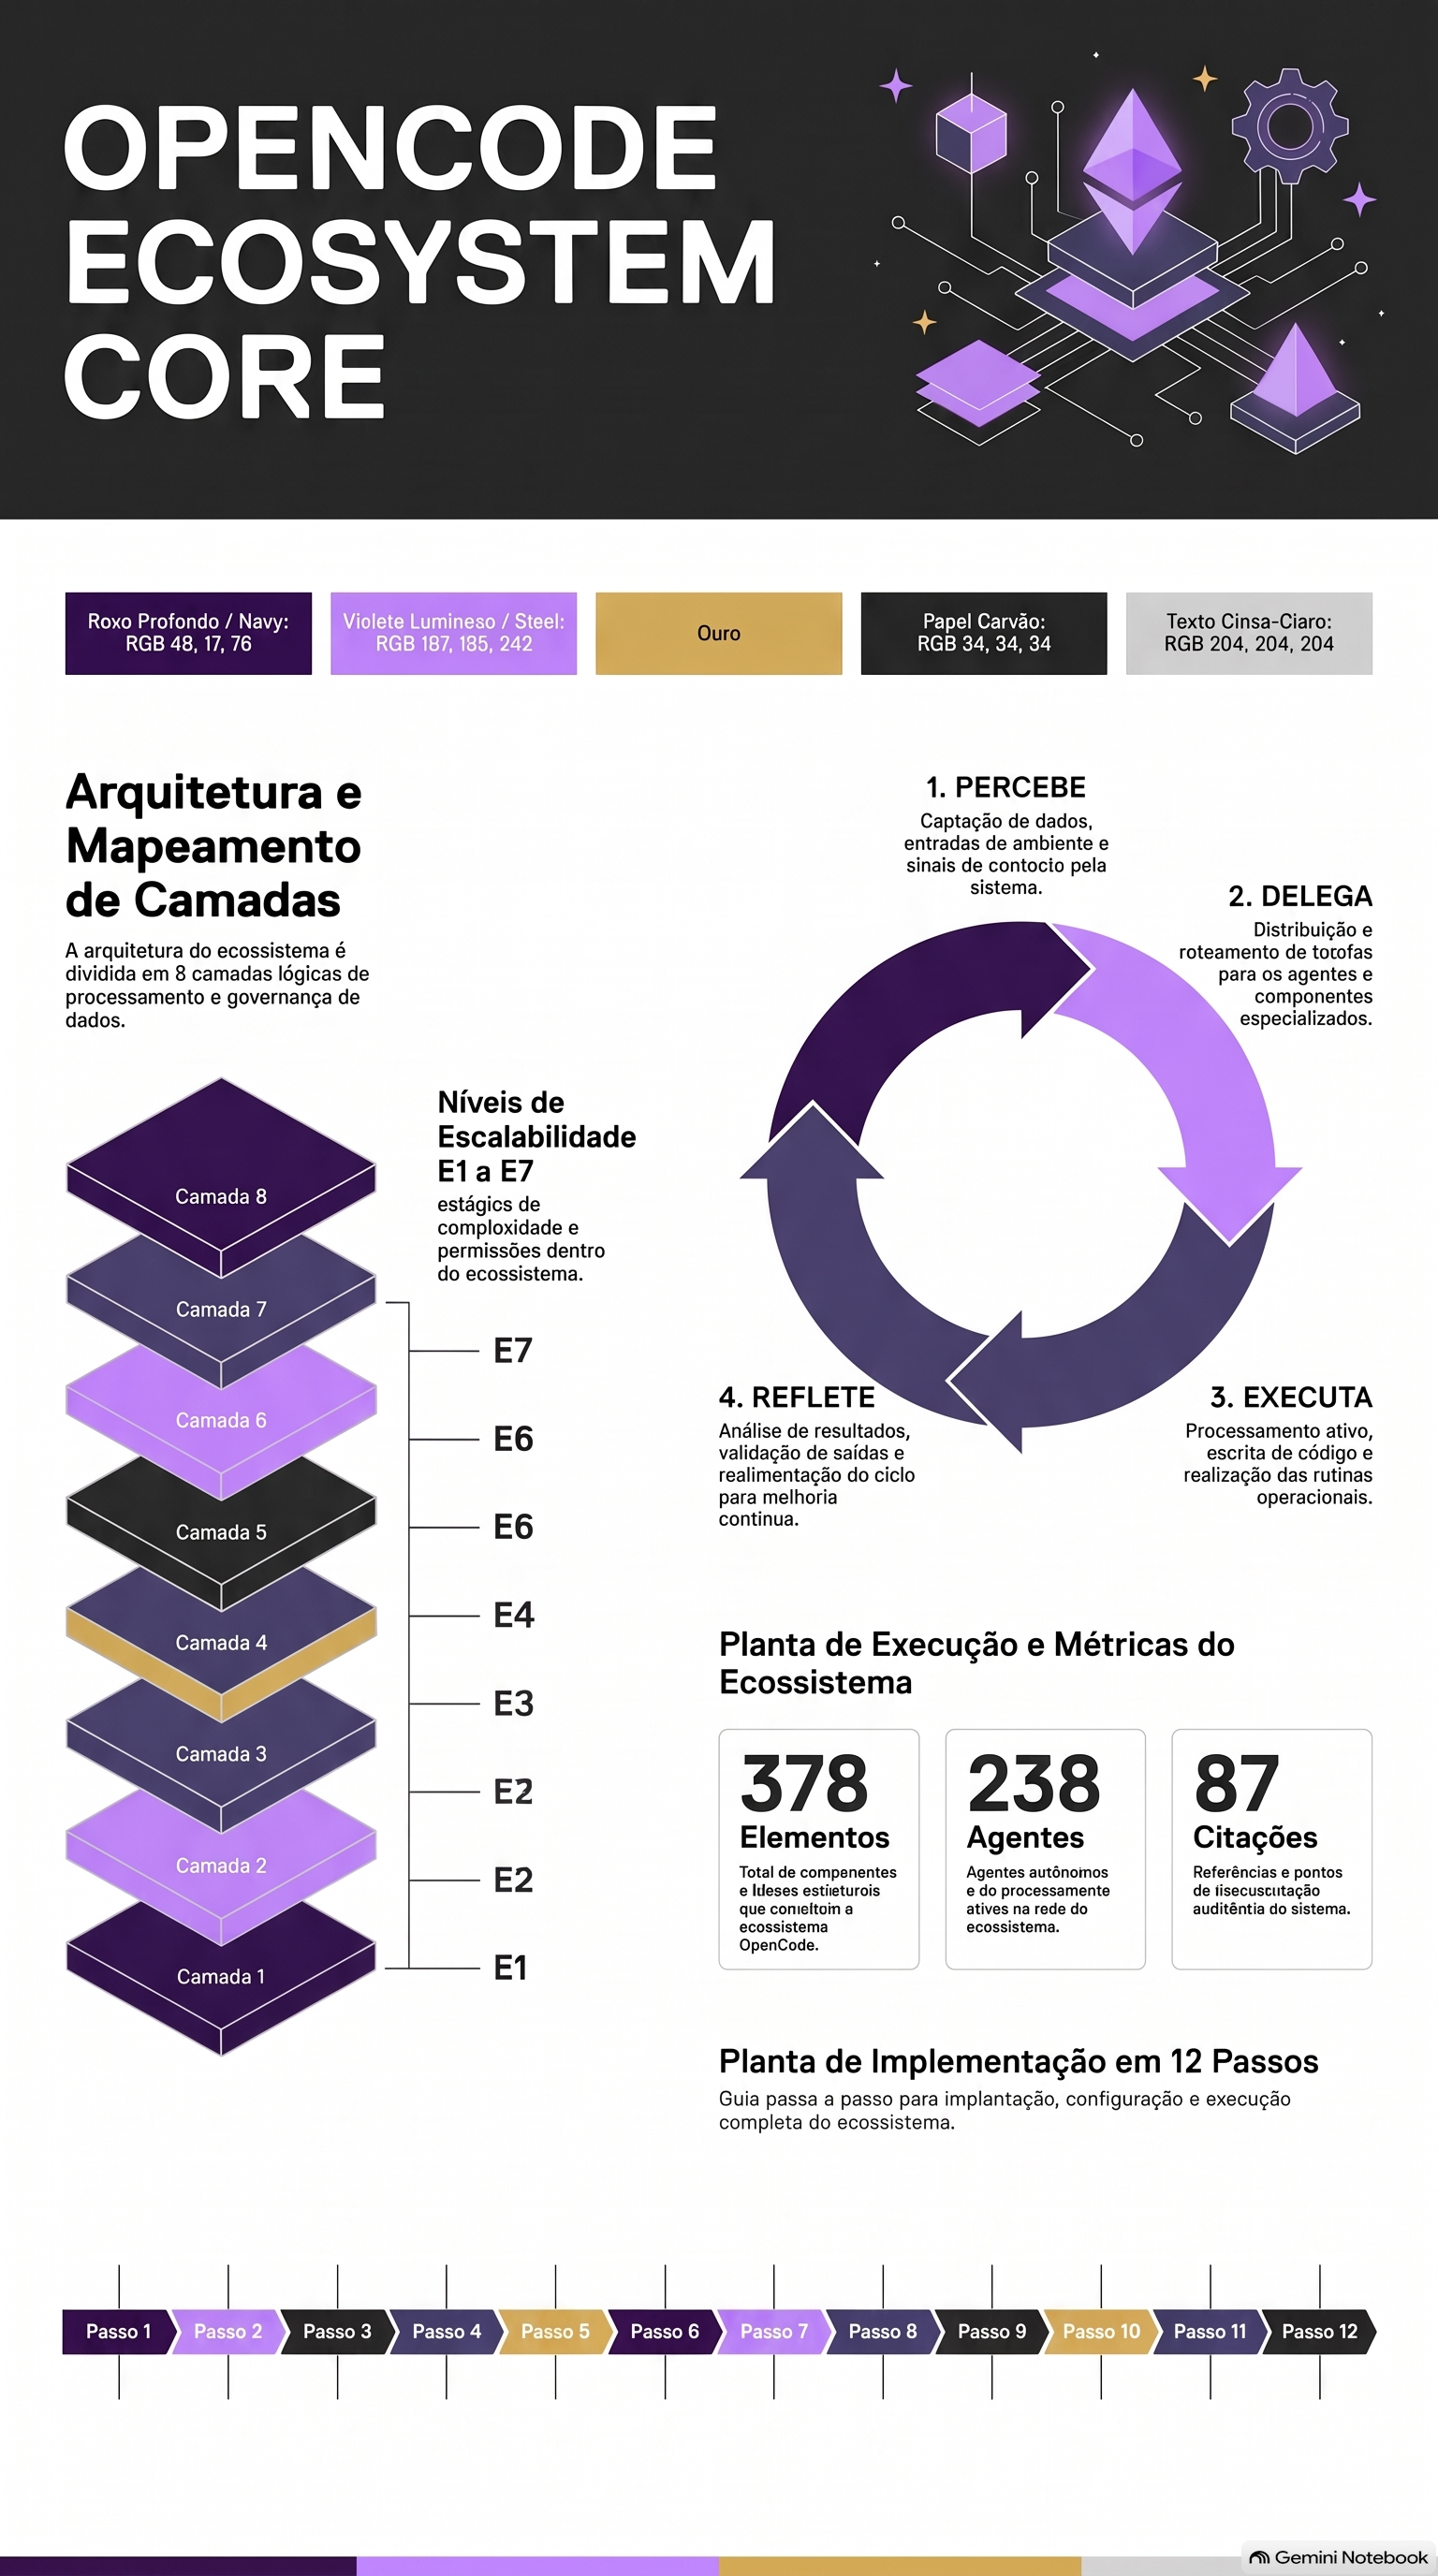
\includegraphics[width=0.92\textwidth]{fig-infografico-core.png}
\caption{Infogr\'afico do Core gerado no NotebookLM em pt-BR a partir da capa oficial: logotipo, paleta com RGB, 8 camadas, ciclo, m\'etricas e planta de 12 passos. Figura ilustrativa: microtextos podem conter trocas de letras do gerador; valem os n\'umeros do texto.}
\end{figure}

\begin{aviso}
Limite do atlas. Os dez mapas cobrem arququetipos por camada e por processo; fichas individuais do catalogo herdam o mapa da sua camada. Mapa algum substitui abrir o arquivo e rodar o comando.
\end{aviso}

% ============================================================
%  MODULO 17 — E1-E7 para leigos: cada paragrafo expandido
%  SPEC R681 — CONTINUAR com NotebookLM (notebook ba4adef8...)
%  NotebookLM: notebook criado, 1 nota, 3 fontes; query confirmou
%  que fontes nao cobrem E1-E7 (resposta honesta registrada).
%  Correcao R681: DOI Nii 10.1609/aimag.v7i2.537 (era .538).
% ============================================================
\chapter{E1 a E7 Para Leigos: O Pedido Andando Pela Casa}

\roteirodidatico
{Este capitulo pega o paragrafo tecnico mais dificil do livro, o bloco de ativacao E1 a E7, e o conta como quem acompanha uma encomenda: quem recebe, quem decide, quem faz, quem confere e quem entrega.}
{\emph{Gatilho} e o pedido escrito; \emph{capacidade} e o que cada ajudante declara saber tentar; \emph{escore} e a nota de casamento entre pedido e ajudante; \emph{gate} e o fiscal que devolve sem nota suficiente.}
{Leia cada E em cinco linhas: Ana ve, Bruno faz, analogia, exemplo e armadilha. So avance quando souber dizer o que confere aquele E.}
{Escore alto e casamento de palavras, nao garantia de acerto. Fiscal reprovando nao e falha do livro: e o livro funcionando.}
{Que papel voce faria nesta casa hoje: quem pede, quem escolhe, quem faz ou quem confere?}

\casoguiado{a encomenda de Ana}
{Ana pede: resuma este artigo em dez linhas sem inventar dados, cada frase com fonte. O pedido entra na portaria, passa pela lousa, chega a quem resume, volta ao fiscal e sai como texto com fontes. Bruno registra cada passagem com hora e responsavel. Se o fiscal devolver, ninguem finge que entregou: anota-se o motivo e tenta-se de novo.}

\section{O mapa de uma pagina antes dos detalhes}

\begin{flowch}[E1-E7 em linguagem da casa]{fonte: mod-02, mod-13 e notebook NotebookLM ba4adef8}
\matrix[matrix of nodes,name=e17,row sep=2.2mm,column sep=2.5mm,nodes={fn},ampersand replacement=\&]{
 |[fns]|E1 Portaria: pedido escrito \\
 |[fn]|E2 Plaquinhas: quem sabe o que \\
 |[fn]|E3 Comparacao: nota de casamento \\
 |[fn]|E4 Lousa: nome de quem faz \\
 |[fn]|E5 Oficina: fazer com ferramenta \\
 |[fde]|E6 Fiscal: passou no criterio \\
 |[fne]|E7 Entrega: resposta com fonte \\
};
\draw[seta] (e17-1-1.south)--(e17-2-1.north);
\draw[seta] (e17-2-1.south)--(e17-3-1.north);
\draw[seta] (e17-3-1.south)--(e17-4-1.north);
\draw[seta] (e17-4-1.south)--(e17-5-1.north);
\draw[seta] (e17-5-1.south)--(e17-6-1.north);
\draw[seta] (e17-6-1.south)--(e17-7-1.north);
\end{flowch}

\begin{descricao}
Guarde este desenho. Cada secao a seguir e um zoom em uma caixa. A seta so anda para frente quando ha registro; volta quando o fiscal manda refazer.
\end{descricao}

\section{E1 -- Gatilho: o pedido precisa estar escrito}

\elemento{E1 Gatilho para leigos}{\metainfo{ID}{E1-LEIGO} \hfill \metainfo{Tecnico}{publica tarefa no Quadro} \hfill \metainfo{Rota}{\pth{mci/blackboard.py}}}

\begin{descricao}
Para Ana: gatilho e o bilhete que ela deixa na portaria. Se o bilhete diz so me ajuda aqui, ninguem sabe o que fazer e o pedido volta. Se diz resuma este artigo em dez linhas com fonte por frase, a casa consegue andar. Para Bruno: E1 transforma texto em tarefa com entrada, criterio e saida esperada, e publica no Quadro Negro. Analogia: e como pedir exame no posto com guia preenchida, nao so dizendo estou mal. Exemplo: tarefa de resumo com dois criterios executaveis, cada frase aponta um trecho. Armadilha: achar que falar com o balcao ja e ativar agente; sem bilhete registrado, nao houve ativacao.
\end{descricao}

\begin{funcao}
Separar vontade de tarefa: so conta como E1 o que ficou escrito, datado e publicado para outros verem.
\end{funcao}

\section{E2 -- Capacidade: quem declara saber o que}

\elemento{E2 Capacidade para leigos}{\metainfo{ID}{E2-LEIGO} \hfill \metainfo{Tecnico}{cartao de agente em \pth{opencode.json}}}

\begin{descricao}
Para Ana: cada ajudante tem uma plaquinha na porta, por exemplo sei buscar fontes ou sei resumir texto dado. Plaquinha nao e diploma: e promessa de tentar. Para Bruno: capacidade e lista declarada em \pth{agents/catalog/} e \pth{opencode.json}, usada para filtrar elegiveis antes de dar nota. Analogia: quadro de plantao no hospital, cada nome com especialidade do dia. Exemplo: pedido com busca exige plaquinha de busca; pedido com documentos prontos pede plaquinha de resumo. Armadilha: confundir plaquinha bonita com prova de qualidade; E2 localiza, nao avalia.
\end{descricao}

\begin{funcao}
Evitar chamar quem nem se propos ao servico: sem casamento de capacidade, nem entra na comparacao.
\end{funcao}

\section{E3 -- Roteamento: dar nota de casamento sem prometer acerto}

\elemento{E3 Roteamento para leigos}{\metainfo{ID}{E3-LEIGO} \hfill \metainfo{Tecnico}{Jaccard e atencao}}

\begin{descricao}
Para Ana: a casa compara as palavras do bilhete com as plaquinhas e da uma nota de parecido. Nota alta quer dizer as palavras combinam, nao que o servico sera otimo. Para Bruno: duas contas aparecem aqui. A simples e Jaccard: entre palavras do pedido $K$ e capacidades $C_{a}$, $A(a) = |K \cap C_{a}|/|K \cup C_{a}|$, com desempate por prioridade de categoria. A fina e atencao ponderada por consulta, chave e historico. Analogia: escolher chave pelo formato da fechadura, sem garantir que abre de primeira.
\end{descricao}

\begin{resultado}
Exemplo com conta. Pedido com palavras resuma, artigo, fonte: $K$ tem 3 itens. Ajudante A declara resuma, texto, fonte: intersecao 2, uniao 4, $A=2/4=0{,}50$. Ajudante B declara busca, artigo, fonte: intersecao 2, uniao 4, $A=0{,}50$. Empate tecnico: decide a prioridade de categoria. Se ninguem passa do minimo, a tarefa fica sem dono e isso e saida legitima, nao erro escondido.
\end{resultado}

\begin{limite}
Nota ordena candidatos elegiveis; nao mede qualidade da entrega nem probabilidade de acerto. O fiscal E6 continua obrigatorio.
\end{limite}

\section{E4 -- Delegacao: escrever na lousa quem faz o que}

\elemento{E4 Delegacao para leigos}{\metainfo{ID}{E4-LEIGO} \hfill \metainfo{Tecnico}{voluntariado e registro}}

\begin{descricao}
Para Ana: depois da nota, o nome do escolhido vai para a lousa grande com a tarefa ao lado, para todos verem e ninguem fazer duplicado. Ha dois jeitos: chamar direto quem e obvio ou anunciar e esperar voluntario com plaquinha compativel. Para Bruno: publicacao de proposta e aceite com registro de atribuicao, trilha auditavel E1 a E7. Analogia: escala de plantao assinada, nao recado de corredor. Exemplo: resumo com busca vai para o buscador primeiro, depois para o resumidor, cada passagem anotada. Armadilha: achar que delegar e executar; E4 so distribui, quem faz e E5.
\end{descricao}

\begin{funcao}
Tornar a escolha visivel e cobravel: sem nome na lousa, ninguem e dono e ninguem responde.
\end{funcao}

\section{E5 -- Execucao: fazer com ferramenta e deixar rastro}

\elemento{E5 Execucao para leigos}{\metainfo{ID}{E5-LEIGO} \hfill \metainfo{Tecnico}{agente mais ferramenta MCP}}

\begin{descricao}
Para Ana: o escolhido faz o servico usando as ferramentas certas, por exemplo abrir o artigo e copiar trechos antes de resumir, sem inventar. Para Bruno: agente executa microtarefa via ferramentas MCP e devolve artefato tipado com logs. Analogia: cozinheiro com receita e ingredientes na bancada, nao de memoria. Exemplo: resumo onde cada frase traz o numero do paragrafo de origem. Armadilha: aceitar texto bonito sem rastro de ferramenta; beleza nao e evidencia.
\end{descricao}

\begin{funcao}
Produzir entrega confrontavel: artefato mais rastro que permita ao fiscal E6 repetir a conferencia.
\end{funcao}

\section{E6 -- Gate: o fiscal que devolve sem pena}

\elemento{E6 Gate para leigos}{\metainfo{ID}{E6-LEIGO} \hfill \metainfo{Tecnico}{fail-closed em \pth{sdd/tdd_runner.py}}}

\begin{descricao}
Para Ana: o fiscal compara a entrega com o bilhete. Faltou fonte, passou de dez linhas ou inventou dado, volta com motivo escrito. Para Bruno: verificacao de especificacao e teste verde; reprovou, nao encerra como concluida e volta para revisao. Analogia: prova com gabarito: nao passou, refaz, sem jeitinho. Exemplo: dois criterios, um falhou, tarefa nao e aprovada por esse contrato e nao se inventa aprovacao. Armadilha: trocar fiscal por torcida; teste verde fora do criterio nao abre gate.
\end{descricao}

\begin{funcao}
Proteger o leitor do acaso: na duvida, reprovar e registrar e melhor que entregar duvidoso como certo.
\end{funcao}

\section{E7 -- Entrega: resposta com fonte e dono}

\elemento{E7 Entrega para leigos}{\metainfo{ID}{E7-LEIGO} \hfill \metainfo{Tecnico}{conclusao com proveniencia}}

\begin{descricao}
Para Ana: so agora o resumo chega as maos dela, com fontes, limites e nome de quem fez e quem conferiu. Ela pode usar na aula e citar sem medo. Para Bruno: encerramento com relatorio de conclusao, memoria atualizada e ciclo registrado quando relevante. Analogia: encomenda com nota fiscal e remetente, nao pacote anonimo. Exemplo: dez linhas, cada uma com trecho de origem, mais nota do que nao foi encontrado. Armadilha: guardar a entrega so na memoria; sem registro, a proxima tarefa comeca do zero.
\end{descricao}

\begin{funcao}
Fechar com responsabilidade: quem recebe sabe o que usar, o que nao usar e a quem perguntar.
\end{funcao}

\begin{flowch}[Conta de Jaccard em um olhar]{fonte: ativ-02o e secao E3 acima}
\matrix[matrix of nodes,name=jac,row sep=3mm,column sep=4mm,nodes={fn},ampersand replacement=\&]{
 |[fns]|Palavras do pedido K \& |[fn]|Plaquinha do agente \\
 |[fn]|Intersecao: o que combina \& |[fn]|Uniao: tudo que apareceu \\
 |[fde]|Nota A igual combina sobre total \& |[fne]|Empate decide categoria \\
};
\draw[seta] (jac-1-1)--(jac-1-2);
\draw[seta] (jac-1-2.south)--(jac-2-2.north);
\draw[seta] (jac-2-1)--(jac-2-2);
\draw[seta] (jac-2-2.south)--(jac-3-1.north);
\draw[seta] (jac-3-1)--(jac-3-2);
\end{flowch}

\begin{aviso}
Limite do capitulo. E1 a E7 e pipeline explicativo, nao promessa de desempenho. Escore mede casamento semantico; gate mede conformidade com criterio; nenhum dos dois mede verdade geral. NotebookLM ajudou a organizar o roteiro leigo e a conferir fontes; a conta e a conferencia final sao locais e repetiveis.
\end{aviso}


\part{Podcast Para Leigos}
% ============================================================
%  MODULO 19 — Podcast: apresentacao consolidada em portugues
%  SPEC R683/R684 — faixa principal PT garantida + episodio NotebookLM
% ============================================================
\chapter{Podcast: O Livro Inteiro em Uma Explica\c{c}\~ao \'{U}nica}

\roteirodidatico
{Este capitulo e o livro falado: o que e o Core, o consolidado de todas as partes, o especial, o limite, a ajuda ao pesquisador e o funcionamento com minucia e justificativa, num equilibrio unico entre leigo e dev.}
{\emph{Apresenta\c{c}\~ao} diz o que e; \emph{consolidado} resume o todo; \emph{especial} mostra a vantagem; \emph{limite} mostra a fronteira; \emph{minucia} abre o mecanismo com conta e motivo.}
{Ou\c{c}a a faixa principal com o roteiro na m\~ao, pause em cada bloco e confira o termo no dicionario nivel 0.}
{Audio resume; prova esta no livro e nas fontes com DOI. Voz gerada pode errar enfase.}
{Que bloco voce reconta sozinho: a casa, os sete passos, o especial ou o limite?}

\casoguiado{Ana e Bruno ouvem juntos}
{Ana ouve a casa e os sete passos e anota: sem fonte, devolve. Bruno ouve Jaccard e PPV e anota as contas para refazer. Os dois terminam sabendo pedir e conferir, cada um no seu nivel.}

\section{As duas faixas e os arquivos}

\elemento{Podcast consolidado em portugues}{\metainfo{ID}{POD-02} \hfill \metainfo{Idioma}{pt-BR} \hfill \metainfo{Pasta}{output/podcast/}}

\begin{descricao}
Faixa principal em portugues, \pth{livro-core-apresentacao-ptbr.mp3}, cerca de quatro minutos, lida do roteiro consolidado \pth{roteiro-consolidado-ptbr.md}: apresenta\c{c}\~ao, consolidado em seis frases, especial, limites, ajuda ao pesquisador e minucia com Jaccard e PPV. Episodio longo do NotebookLM em pt-BR, \pth{livro-core-notebooklm-ptbr.m4a}, cerca de vinte minutos, gerado no caderno em portugues com idioma forcado a partir das quatro fontes em portugues. Apoio: sintese do caderno, nove cartoes e feed com tamanho real. Para refazer a faixa PT, rode o gerador de voz sobre o roteiro; para o episodio, crie o audio no caderno com idioma pt-BR e foco consolidado, depois baixe o audio.
\end{descricao}

\begin{funcao}
Uma explica\c{c}\~ao unica com dois ritmos: quatro minutos para situar-se, vinte para aprofundar, ambos terminando no mesmo dicionario e na mesma planta de doze passos.
\end{funcao}

\section{O consolidado em seis blocos para recontar}

\begin{descricao}
Um, o que e: casa com porteiro unico, 378 elementos e regra dura de combinado e teste. Dois, o livro em seis frases: prologo, quatro esta\c{c}\~oes, oito camadas, sete passos, memoria que aprende, qualidade e reprodu\c{c}\~ao. Tres, o especial: balcao que coordena, lousa voluntaria, caderno que vira erro em criterio, fiscal e proveni\^encia. Quatro, o limite: nota e parecido, teste e criterio, sem selo sem externa. Cinco, o pesquisador: fontes, resumo sem inventar, metodo e auditoria ate o DOI. Seis, a minucia: E1 a E7 com Jaccard e aten\c{c}\~ao, risco de 89 por cento em 216 saidas e PPV de 62 por cento em campo dificil, conferidos com doctor e recompila\c{c}\~ao.
\end{descricao}

\begin{aviso}
Limite do audio. Em divergencia entre ouvido e impresso, vale o impresso com a fonte citada. Nenhuma faixa promete sotaque, trilha ou dura\c{c}\~ao exata em outro gerador.
\end{aviso}

% ============================================================
%  MODULO 20 — Podcast por modulo: indice de episodios
%  SPEC R686 — um audio curto pt-BR por modulo (fila progressiva)
% ============================================================
\chapter{Podcast Por M\'odulo: Ou\c{c}a Cada Parte}

\roteirodidatico
{Se um capitulo ficou denso, ou\c{c}a o episodio dele. Cada modulo do livro tem um audio curto em portugues com detalhe, funcionalidade, justificativa, intera\c{c}\~oes, agentes, specs e hooks.}
{\emph{Episodio por modulo} aprofunda uma parte; \emph{consolidado} apresenta o todo. Ou\c{c}a o todo antes das partes.}
{Escolha o modulo travado, ou\c{c}a o episodio com a ficha aberta e pause para conferir arquivo e comando.}
{Audio resume fontes do caderno; prova esta no texto e no DOI. Fila de gera\c{c}\~ao respeita a cota do plano.}
{Que modulo voce ouve hoje, e que detalhe dele voce reconta depois?}

\casoguiado{Bruno destrava o roteamento}
{Bruno trava no roteamento por aten\c{c}\~ao. Ouve os seis minutos do modulo 02 com o fluxograma M6 aberto, pausa no Jaccard, refaz a conta 2 sobre 4 e volta ao codigo. Destrava sem reler o capitulo inteiro.}

\section{Episodios prontos e fila}

\elemento{\'Indice de episodios por modulo}{\metainfo{ID}{PODM-01} \hfill \metainfo{Idioma}{pt-BR curto} \hfill \metainfo{Pasta}{output/podcast/modulos/}}

\begin{descricao}
Prontos: 02 orquestra\c{c}\~ao E1-E7, 03 memoria MCI, 04 qualidade SDD e TDD, 05 raciocinio, 07 integra\c{c}\~oes com MCP e executores, 10 catalogo com 238 agentes em 14 familias, 13 ativa\c{c}\~ao com trilha auditavel. Gerando: 01 funda\c{c}\~oes e 06 ci\^encia. Fila apos renovar a cota: 00a prologo, 00b jornada, 01b historia, 01c instala\c{c}\~ao, 01d arquitetura, 08 ecossistema, 09 infra, 09a comparada, 12 fichas nucleo, 14 lotes, 15 epilogo, 16 atlas, 17 E1-E7 leigo, 18 nivel 0 e 19 podcast. Cada episodio traz detalhe, funcionalidade, justificativa com DOI, intera\c{c}\~oes, agentes e subagentes, specs, hooks e ferramentas do modulo. Para gerar a fila, crie o audio no caderno por modulo com idioma pt-BR e foco do modulo, depois baixe para a pasta de modulos.
\end{descricao}

\begin{funcao}
Transformar cada capitulo denso em conversa curta, sem perder rastro: o episodio aponta a ficha, a ficha aponta o arquivo.
\end{funcao}

\begin{aviso}
Limite dos episodios. Audio gerado pode simplificar nomes e numeros; o numero que vale e o recalculado no checkout. Cota do plano limita a fila: episodios restantes saem apos renovar a janela.
\end{aviso}


\part{Epílogo Operacional — Reprodução Guiada}
% ============================================================
%  MODULO 15 — Epilogo operacional: Reproduza o Core em 12 passos
%  SPEC R679 — planta executavel, calculos C1-C4 fechados
% ============================================================
\chapter{Ep\'ilogo Operacional: Reproduza o Core em Doze Passos}

\roteirodidatico
{Ana quer ter certeza de que o que leu continua valendo amanh\~a; Bruno quer provar que consegue reconstruir tudo em outra m\'aquina. Este ep\'ilogo \'e a planta que os dois executam juntos, cada passo com comando, sa\'ida esperada e modo de conferir.}
{\emph{Proveni\^encia} diz quem gerou, de que vers\~ao e com que comando; \emph{fotografia} \'e contagem datada do checkout; \emph{gate} \'e teste booleano que reprova na d\'uvida; \emph{hash} \'e impress\~ao digital do arquivo.}
{Execute na ordem, anote a sa\'ida real ao lado da esperada e pare no primeiro desvio para diagnosticar antes de seguir.}
{Reproduzir prova que o caminho \'e percorr\'ivel, n\~ao que toda resposta do sistema \'e correta. N\'umero de teste verde n\~ao \'e medida de verdade geral.}
{Que passo desta planta voc\^e consegue executar agora, com que evid\^encia, e qual depend\^encia externa ainda pode impedi-lo?}

\casoguiado{Bruno reconstr\'oi, Ana confere}
{Bruno clona o reposit\'orio, cria o ambiente virtual e roda o diagn\'ostico. Ana anota num caderno: quantos agentes o arquivo declara, quantas specs carregaram, quantos testes passaram. Quando o PDF recompila, os dois comparam o n\'umero de p\'aginas e o sum\'ario com a edi\c{c}\~ao que leram. Se algum n\'umero divergir, n\~ao concluem que o livro mentiu: concluem que o checkout mudou e registram a nova fotografia com data.}

\section{Planta de doze passos com confer\^encia}

A planta trata o ambiente, o c\'odigo e os dados como parte do relato, n\~ao como anexo. Essa exig\^encia vem da ci\^encia computacional reproduz\'ivel, que pede o artigo acompanhado do ambiente completo.

Sem o ambiente, o artigo descreve inten\c{c}\~ao; com ele, outro pesquisador pode percorrer o mesmo caminho e comparar resultados \citref{PENG, R. D. Reproducible research in computational science. Science, v.~334, n.~6060, p.~1226-1227, 2011}{10.1126/science.1213847}{Exige que este epilogo entregue comandos e versoes como parte do texto cientifico, nao como anexo opcional.}{Reproducible research is the idea that the ultimate product of academic research is the paper along with the full computational environment}{Pesquisa reproduzivel e a ideia de que o produto final da pesquisa academica e o artigo junto com o ambiente computacional completo.}{PENG, 2011, p.~1226-1227}.

Cada entrega desta planta carrega proveni\^encia para ser encontrada, acessada e reutilizada por pessoas e m\'aquinas, segundo os princ\'ipios de dados justos.

A infraestrutura de reutiliza\c{c}\~ao \'e a condi\c{c}\~ao para que a reprodu\c{c}\~ao de hoje sirva \`a auditoria de amanh\~a \citref{WILKINSON, M. D. et al. The FAIR Guiding Principles for scientific data management and stewardship. Scientific Data, v.~3, 160018, 2016}{10.1038/sdata.2016.18}{Fundamenta a exigencia de proveniencia por observacao em cada passo da planta: identificador, descricao e registro.}{There is an urgent need to improve the infrastructure supporting the reuse of scholarly data}{Ha uma necessidade urgente de melhorar a infraestrutura que sustenta a reutilizacao de dados academicos.}{WILKINSON et al., 2016, 160018}.

\elemento{Planta em doze passos}{\metainfo{ID}{REP-12} \hfill \metainfo{Tempo}{cerca de uma tarde} \hfill \metainfo{Gate}{parar no primeiro desvio}}

\begin{descricao}
Passos 1 a 4 preparam o terreno. Passo 1: clone ou atualize o reposit\'orio e anote o hash do commit. Passo 2: crie o ambiente virtual Python 3 e ative-o. Passo 3: instale com \pth{make install} e \pth{make setup}, depois \pth{make setup-dev} ou \pth{make setup-science} se precisar. Passo 4: rode \pth{python3 -m marceloclaro.cli doctor} e guarde as 20 linhas de veredito. Esperado: specs formais carregadas, registro de evolu\c{c}\~ao \'integro, mem\'oria acess\'ivel. Se faltar CLI externa, o diagn\'ostico avisa em amarelo; anote como depend\^encia opcional ausente, n\~ao como falha total.
\end{descricao}

\begin{descricao}
Passos 5 a 8 conferem o invent\'ario. Passo 5: conte agentes em \pth{opencode.json}, chave \pth{agent}; confira o total com o M\'odulo 10. Passo 6: conte arquivos \pth{specs/SPEC-935-R*.md} e compare com o n\'umero que o \pth{doctor} diz ter carregado; escopos distintos explicam diferen\c{c}as. Passo 7: conte arquivos e linhas em \pth{mci/} e anote como fotografia datada. Passo 8: rode a su\'ite m\'inima de testes do n\'ucleo e anote verdes e vermelhos. Nenhuma dessas contagens mede qualidade; todas medem presen\c{c}a naquela vers\~ao.
\end{descricao}

\begin{descricao}
Passos 9 a 12 fecham o ciclo. Passo 9: execute uma tarefa de brinquedo pelo Orquestrador e guarde Blackboard, escore e gate. Passo 10: confira cada DOI deste livro abrindo \pth{https://doi.org/} mais o sufixo; DOI que n\~ao resolve n\~ao entra na pr\'oxima edi\c{c}\~ao. Passo 11: recompile com \pth{pdflatex main.tex} dentro de \pth{livro-core/} e rode \pth{python3 check.py}; esperado \pth{ok} e \pth{main.pdf} regenerado. Passo 12: registre ciclo de evolu\c{c}\~ao e li\c{c}\~ao no MetaBus com data, hash e o que mudou. Sem passo 12, a reprodu\c{c}\~ao serviu s\'o a voc\^e; com ele, serve ao pr\'oximo leitor.
\end{descricao}

\begin{funcao}
Transformar leitores em replicadores: cada passo deixa rastro que outro pode seguir, comparar e contestar, sem depender da m\'aquina do autor.
\end{funcao}

\section{Quatro c\'alculos fechados para levar no bolso}

Primeiro c\'alculo, risco de agregar sem gate. Com $N=216$ e $p=0{,}99$, $P=1-0{,}99^{216}\approx 0{,}886$. Variante com $p=0{,}999$: $\ln(0{,}999^{216})=216\ln 0{,}999\approx 216\times(-0{,}0010005)\approx -0{,}216$, logo $0{,}999^{216}\approx e^{-0{,}216}\approx 0{,}806$ e $P\approx 0{,}194$, cerca de 19 por cento. Melhorar cada pe\c{c}a de 99 para 99,9 por cento derruba o risco de 89 para 19 por cento, mas n\~ao o zera. A hip\'otese de independ\^encia segue fr\'agil: erros correlacionados quebram a f\'ormula para cima.

Segundo c\'alculo, aten\c{c}\~ao de brinquedo, j\'a resolvido na jornada: com $QK^{T}=[[4,0],[0,4]]$ e $d_{k}=4$, softmax d\'a $[0{,}88,0{,}12]$ e $[0{,}12,0{,}88]$. A li\c{c}\~ao permanece: peso concentra onde o escore destaca, e escore empatado divide.

Terceiro c\'alculo, valor preditivo positivo. Com $R=0{,}1$, poder $0{,}8$ e $\alpha=0{,}05$, $\mathrm{PPV}\approx 0{,}615$. Com campo f\'acil $R=1$, $\mathrm{PPV}=0{,}8/(0{,}8+0{,}05)\approx 0{,}941$. O mesmo teste verde vale 62 por cento num campo e 94 por cento noutro. A taxa-base manda tanto quanto o teste.

Essa depend\^encia da taxa-base e do vi\'es \'e a raz\~ao formal do anti-overclaim deste livro: sem relatar poder, vi\'es e campo, signific\^ancia n\~ao sustenta proclama\c{c}\~ao.

Para muitos desenhos e campos, a alega\c{c}\~ao tem mais chance de ser falsa do que verdadeira, e \'e por isso que cada ficha termina com limites \citref{IOANNIDIS, J. P. A. Why most published research findings are false. PLoS Medicine, v.~2, n.~8, e124, 2005}{10.1371/journal.pmed.0020124}{Fecha os tres calculos com a formula do PPV: taxa-base, poder e vies decidem o que um teste verde permite concluir.}{Simulations show that for most study designs and settings, it is more likely for a research claim to be false than true}{Simulacoes mostram que, para a maioria dos desenhos e cenarios de estudo, e mais provavel que uma alegacao de pesquisa seja falsa do que verdadeira.}{IOANNIDIS, 2005, e124}.

Quarto c\'alculo, invent\'ario reproduz\'ivel. Rode no raiz do reposit\'orio o trio: contagem de agentes por chave \pth{agent} em \pth{opencode.json}, contagem de \pth{specs/SPEC-935-R*.md} e contagem de arquivos em \pth{mci/}. Anote os tr\^es n\'umeros com data e hash do commit. Repita ap\'os cada \pth{git pull}. Se o \pth{doctor} disser 160 specs carregadas e a pasta tiver 321 arquivos, n\~ao h\'a contradi\c{c}\~ao: um conta registros reconhecidos, outro conta arquivos presentes. A disciplina de passos curtos e uniformes \'e o que torna essas contagens confi\'aveis como rotina.

Ciclos curtos intercalados com testes mant\^em o foco e permitem localizar a diverg\^encia no passo em que ela nasceu, em vez de ca\c{c}\'a-la no fim \citref{FUCCI, D. et al. A dissection of the test-driven development process: does it really matter to test-first or to test-last? IEEE Transactions on Software Engineering, v.~43, n.~7, p.~597-614, 2017}{10.1109/TSE.2016.2616877}{Justifica o quarto calculo como rotina curta e uniforme: conferir inventario a cada mudanca em vez de auditar tudo no fim.}{Test-driven development is a technique that repeats short coding cycles interleaved with testing}{Desenvolvimento orientado a testes e uma tecnica que repete ciclos curtos de codificacao intercalados com testes.}{FUCCI et al., 2017, p.~597-614}.

\section{Despedida de Ana e Bruno}

Ana fecha o caderno e diz que agora sabe pedir sem ser enganada: com fonte, com limite e com direito a devolver. Bruno fecha o terminal e diz que agora sabe entregar sem enganar: com spec, com teste e com proveni\^encia. O narrador despede-se com a mesma frase que abriu o pr\'ologo: neste livro, hist\'oria alguma substitui arquivo, e arquivo algum dispensa verifica\c{c}\~ao. O pr\'oximo leitor que refizer os doze passos e recalcular os quatro c\'alculos ser\'a o pr\'oximo autor da pr\'oxima fotografia datada.

\begin{aviso}
Limite do ep\'ilogo. A planta foi testada neste checkout em 05/10/2026; depend\^encias externas, credenciais de provedores e modelos locais podem mudar o resultado em outra m\'aquina. Guardar sa\'idas reais ao lado das esperadas \'e parte da reprodu\c{c}\~ao, n\~ao ap\^endice.
\end{aviso}

\section{Refer\^encias did\'aticas desta jornada com acesso em 05 out.~2026}

\begin{referencia}
\textbf{SWELLER, J.} Cognitive load during problem solving: effects on learning. \emph{Cognitive Science}, v.~12, n.~2, p.~257-285, 1988. DOI: \href{https://doi.org/10.1016/0364-0213(88)90023-7}{10.1016/0364-0213(88)90023-7}. Uso: metodo didatico do livro, exemplos antes do formalismo.
\end{referencia}

\begin{referencia}
\textbf{FLAVELL, J. H.} Metacognition and cognitive monitoring. \emph{American Psychologist}, v.~34, n.~10, p.~906-911, 1979. DOI: \href{https://doi.org/10.1037/0003-066X.34.10.906}{10.1037/0003-066X.34.10.906}. Uso: MetaBus como monitoramento cognitivo.
\end{referencia}

\begin{referencia}
\textbf{NII, H. P.} Blackboard systems. \emph{AI Magazine}, v.~7, n.~2, p.~38-53, 1986. DOI: \href{https://doi.org/10.1609/aimag.v7i2.537}{10.1609/aimag.v7i2.537}. Uso: Quadro Negro A2A.
\end{referencia}

\begin{referencia}
\textbf{WOOLDRIDGE, M.; JENNINGS, N. R.} Intelligent agents: theory and practice. \emph{The Knowledge Engineering Review}, v.~10, n.~2, p.~115-152, 1995. DOI: \href{https://doi.org/10.1017/S0269888900008122}{10.1017/S0269888900008122}. Uso: definicao de agente.
\end{referencia}

\begin{referencia}
\textbf{VASWANI, A. et al.} Attention is all you need. \emph{Advances in Neural Information Processing Systems}, v.~30, p.~5998-6008, 2017. DOI: \href{https://doi.org/10.48550/arXiv.1706.03762}{10.48550/arXiv.1706.03762}. Uso: roteamento por atencao.
\end{referencia}

\begin{referencia}
\textbf{IOANNIDIS, J. P. A.} Why most published research findings are false. \emph{PLoS Medicine}, v.~2, n.~8, e124, 2005. DOI: \href{https://doi.org/10.1371/journal.pmed.0020124}{10.1371/journal.pmed.0020124}. Uso: PPV e anti-overclaim.
\end{referencia}

\begin{referencia}
\textbf{WILKINSON, M. D. et al.} The FAIR Guiding Principles. \emph{Scientific Data}, v.~3, 160018, 2016. DOI: \href{https://doi.org/10.1038/sdata.2016.18}{10.1038/sdata.2016.18}. Uso: proveniencia e reuso.
\end{referencia}

\begin{referencia}
\textbf{PENG, R. D.} Reproducible research in computational science. \emph{Science}, v.~334, n.~6060, p.~1226-1227, 2011. DOI: \href{https://doi.org/10.1126/science.1213847}{10.1126/science.1213847}. Uso: planta executavel.
\end{referencia}

\begin{referencia}
\textbf{FUCCI, D. et al.} A dissection of the TDD process. \emph{IEEE Transactions on Software Engineering}, v.~43, n.~7, p.~597-614, 2017. DOI: \href{https://doi.org/10.1109/TSE.2016.2616877}{10.1109/TSE.2016.2616877}. Uso: granularidade e uniformidade.
\end{referencia}

\begin{referencia}
\textbf{RAFIQUE, Y.; MISIC, V. B.} The effects of TDD: a meta-analysis. \emph{IEEE Transactions on Software Engineering}, v.~39, n.~6, p.~835-856, 2013. DOI: \href{https://doi.org/10.1109/TSE.2012.28}{10.1109/TSE.2012.28}. Uso: limite do que TDD promete.
\end{referencia}


% =========================== BACK MATTER ==============================
\appendix
\part{Apêndices e Índices}
% ======================================================================
%  MÓDULO 11 — Referências auditadas e metodologia de citação
%  Regra R110: DOI citado deve ser ativo e verificado externamente.
% ======================================================================
\thispagestyle{fancy}
\chapter{Referências Auditadas e Metodologia de Citação}

\roteirodidatico
{Uma citação permite ao leitor localizar a fonte usada em uma afirmação. Para servir a esse propósito, a referência precisa estar completa e a fonte precisa sustentar o trecho associado.}
{\emph{DOI} identifica um objeto digital; \emph{citação direta} reproduz palavras da fonte; \emph{paráfrase} reformula a ideia; \emph{ABNT} define padrões bibliográficos adotados no manuscrito.}
{Confira autor, título, veículo, ano e localização; abra a fonte; confronte texto original, tradução e afirmação; registre data e método de acesso.}
{Um DOI resolvível confirma a localização do registro, não a interpretação nem a pertinência da citação. Traduções são identificadas como livres e alegações devem permanecer dentro do escopo da fonte.}
{Um leitor consegue encontrar a fonte e verificar, sem depender da interpretação do autor, a afirmação citada e sua localização?}

\casoguiado{conferir uma citação}
{Diante de ``(SOBRENOME, ano, p. 12)'', localize a referência completa, abra a edição citada e confira a página. Se for uma paráfrase, compare a ideia e preserve suas qualificações; se for citação direta, confira cada palavra e o localizador. Um DOI pode levar ao artigo, mas não necessariamente à página citada ou ao texto integral.}

\begin{resultado}
Toda citação com DOI deste manual segue a regra \textbf{R110}/\textbf{anti-overclaim}
(\emph{AGENTS.md}, item 4): nenhum DOI é citado ``de memória''. Antes de entrar
no texto, a referência é \textbf{verificada por consulta externa} (webfetch do
resumo/página do periódico ou do repositório da editora), o \textbf{trecho
original} é copiado literalmente do documento e sua \textbf{tradução livre}
para o português é rotulada como tal. Um DOI que não resolve em
\pth{https://doi.org} ou cujo trecho não confere com a fonte \textbf{não entra}
no livro. Verificação corrente: \textbf{29 de setembro de 2026}.

\textbf{Normas ABNT atualizadas.} As referências seguem a
\textbf{ABNT NBR 6023:2018} (Informação e documentação --- Referências:
elaboração) e as citações seguem a \textbf{ABNT NBR 10520:2023} (Informação e
documentação --- Citações em documentos: apresentação). Adota-se o
\textbf{sistema numérico}: a chamada no texto é a remissão à nota de rodapé, que
traz a \textbf{referência completa} em ABNT, o DOI com \textbf{data de acesso}
e, quando há citação direta, o \textbf{trecho textual} e sua página.
\end{resultado}

\section{Biblioteca de referências auditadas}

\begin{referencia}
\textbf{FLAVELL, J. H.} Metacognition and cognitive monitoring: A new area of
cognitive-developmental inquiry. \emph{American Psychologist}, v.~34, n.~10,
p.~906-911, 1979. DOI: \href{https://doi.org/10.1037/0003-066X.34.10.906}{10.1037/0003-066X.34.10.906}. Acesso em: 29 set. 2026.
\textbf{Uso no manual:} Módulo 3 (definição de conhecimento metacognitivo
persistido no MetaBus). \textbf{Status:} DOI ativo; resumo conferido na fonte
original (Stanford/Sage, out.~1979).
\end{referencia}

\begin{referencia}
\textbf{NII, H. P.} Blackboard systems: The blackboard model of problem solving
and the evolution of blackboard architectures. \emph{AI Magazine}, v.~7, n.~2,
1986. DOI: \href{https://doi.org/10.1609/aimag.v7i2.537}{10.1609/aimag.v7i2.537}. Acesso em: 29 set. 2026.
\textbf{Uso no manual:} Módulo 3 (proveniência do padrão blackboard/A2A e do
vocabulário quadro--fonte de conhecimento). \textbf{Status:} DOI ativo; resumo
conferido no AAIAI Magazine; relato do HEARSAY-II (1971--1976) confirmado.
\end{referencia}

\begin{referencia}
\textbf{IOANNIDIS, J. P. A.} Why most published research findings are false.
\emph{PLoS Medicine}, v.~2, n.~8, e124, 2005. DOI:
\href{https://doi.org/10.1371/journal.pmed.0020124}{10.1371/journal.pmed.0020124}. Acesso em: 29 set. 2026.
\textbf{Uso no manual:} Módulos 3 e 6 (fundamento empírico do gate
\cod{no_verified_without_external} e da regra anti-overclaim).
\textbf{Status:} DOI ativo; versão integral acessível em acesso aberto
(PubMed Central PMC1182327); simulações e PPV conferidos no texto integral.
\end{referencia}

\begin{referencia}
\textbf{WILKINSON, M. D.; DUMONTIER, M.; AALBERSBERG, I. J. et al.} The FAIR
Guiding Principles for scientific data management and stewardship.
\emph{Scientific Data}, v.~3, 160018, 2016. DOI:
\href{https://doi.org/10.1038/sdata.2016.18}{10.1038/sdata.2016.18}. Acesso em: 29 set. 2026.
\textbf{Uso no manual:} Módulos 4 e 5 (proveniência defensável dos registros de
execução e reprodutibilidade do patrimônio de specs/testes).
\textbf{Status:} DOI ativo; princípios F/A/I/R (incl. R1.2 proveniência) e
licença CC BY 4.0 conferidos no artigo original (Nature Portfolio).
\end{referencia}

\begin{referencia}
\textbf{WOOLDRIDGE, M.; JENNINGS, N. R.} Intelligent agents: theory and
practice. \emph{The Knowledge Engineering Review}, v.~10, n.~2, p.~115-152,
1995. DOI:
\href{https://doi.org/10.1017/S0269888900008122}{10.1017/S0269888900008122}. Acesso em: 29 set. 2026.
(4093 citações indexadas no Crossref em 29/09/2026; resumo conferido.)
\end{referencia}

\begin{referencia}
\textbf{JENNINGS, N. R.; SYCARA, K.; WOOLDRIDGE, M.} A roadmap of agent
research and development. \emph{Autonomous Agents and Multi-Agent Systems},
v.~1, n.~1, p.~7-38, 1998. DOI:
\href{https://doi.org/10.1023/A:1010090405266}{10.1023/A:1010090405266}. Acesso em: 29 set. 2026.
(Objetivo conforme resumo em Semantic Scholar: identificar conceitos-chave e
aplicações e sua relação mútua.)
\end{referencia}

\begin{referencia}
\textbf{PENG, R. D.} Reproducible research in computational science.
\emph{Science}, v.~334, n.~6060, p.~1226-1227, 2011. DOI:
\href{https://doi.org/10.1126/science.1213847}{10.1126/science.1213847}. Acesso em: 29 set. 2026.
(1157 citações indexadas no Crossref em 29/09/2026; resumo conferido.)
\end{referencia}

\begin{referencia}
\textbf{SMITH, R. G.} The contract net protocol: high-level communication and
control in a distributed problem solver. \emph{IEEE Transactions on Computers},
v.~C-29, n.~12, p.~1104-1113, 1980. DOI:
\href{https://doi.org/10.1109/TC.1980.1675516}{10.1109/TC.1980.1675516}. Acesso em: 29 set. 2026.
\textbf{Uso no manual:} Módulos 2, 7 e 14 (gerência/contratante do Blackboard e
das bridges de integração). \textbf{Status:} DOI ativo; resumo conferido em
\pth{reidgsmith.com}; a licitação e a negociação de contrato conferidas no
texto integral disponível. (Não confundir com o DOI
10.1109/TC.1980.1675514, que é o artigo de Gonzalez \& Jordan sobre avaliação
quantitativa de sistemas distribuídos.)
\end{referencia}

\begin{referencia}
\textbf{BROOKS, F. P. Jr.} No silver bullet: essence and accidents of software
engineering. \emph{Computer}, v.~20, n.~4, p.~10-19, 1987. DOI:
\href{https://doi.org/10.1109/MC.1987.1663532}{10.1109/MC.1987.1663532}. Acesso em: 29 set. 2026.
\textbf{Uso no manual:} Módulo 4 (justificativa do protocolo SDD/TDD como
disciplina acumulada, não bala de prata). \textbf{Status:} DOI ativo; 1804
citações indexadas no Crossref em 29/09/2026; trecho de p.~11 conferido no
texto integral (cópias abertas do \emph{Computer}).
\end{referencia}

\begin{referencia}
\textbf{PAGE, M. J. et al.} PRISMA 2020 explanation and elaboration: updated
guidance and exemplars for reporting systematic reviews. \emph{BMJ}, v.~372,
n160, 2021. DOI:
\href{https://doi.org/10.1136/bmj.n160}{10.1136/bmj.n160}. Acesso em: 29 set. 2026.
\textbf{Uso no manual:} Módulos 6, 11 e 14 (relato transparente de revisões e
da biblioteca de citações). \textbf{Status:} DOI ativo; 9559 citações
indexadas no Crossref em 29/09/2026; resumo conferido na página do BMJ.
(Companion do relato de princípios: DOI 10.1136/bmj.n71.)
\end{referencia}

\begin{referencia}
\textbf{AMDAHL, G. M.} Validity of the single processor approach to achieving
large scale computing capabilities. In: \emph{AFIPS Conference Proceedings},
v.~30, p.~483-485, 1967. DOI:
\href{https://doi.org/10.1145/1465482.1465560}{10.1145/1465482.1465560}. Acesso em: 29 set. 2026.
\textbf{Uso no manual:} Módulos 5 e 14 (limite da aceleração paralela do
pipeline/roteamento). \textbf{Status:} DOI ativo; trecho de p.~484 conferido
no fac-símile do texto integral (arquivo CMU); citação canônica da Lei de
Amdahl.
\end{referencia}

\begin{referencia}
\textbf{SIMON, H. A.} A behavioral model of rational choice. \emph{The
Quarterly Journal of Economics}, v.~69, n.~1, p.~99-118, 1955. DOI:
\href{https://doi.org/10.2307/1884852}{10.2307/1884852}. Acesso em: 29 set. 2026.
\textbf{Uso no manual:} Módulos 8 e 14 (racionalidade limitada como base da
decisão assistida por agentes). \textbf{Status:} DOI ativo; 10407 citações
indexadas no Crossref em 29/09/2026; trecho de p.~99 conferido no texto
integral (JSTOR, acesso legitimado).
\end{referencia}

\begin{referencia}
\textbf{NEWELL, A.} The knowledge level. \emph{Artificial Intelligence},
v.~18, n.~1, p.~87-127, 1982. DOI:
\href{https://doi.org/10.1016/0004-3702(82)90012-1}{10.1016/0004-3702(82)90012-1}. Acesso em: 29 set. 2026.
\textbf{Uso no manual:} Módulo 14 (o agente descrito no nível do conhecimento,
acima do nível simbólico). \textbf{Status:} DOI ativo; trecho do resumo
(p.~87) conferido na página do periódico. (Nota: o sufixo correto é
\cod{90012-1}; \cod{90012-2} não resolve.)
\end{referencia}

\begin{referencia}
\textbf{NELSON, T. O.; NARENS, L.} Metamemory: a theoretical framework and new
findings. In: BOWER, G. H. (ed.). \emph{The Psychology of Learning and
Motivation}. Academic Press, v.~26, p.~125-173, 1990. DOI:
\href{https://doi.org/10.1016/S0079-7421(08)60053-5}{10.1016/S0079-7421(08)60053-5}. Acesso em: 29 set. 2026.
\textbf{Uso no manual:} Módulo 3 (monitoramento e controle do MetaBus).
\textbf{Status:} DOI ativo após auditoria da sessão R613; recorte do resumo do
capítulo (p.~125) conferido na página da editora; é capítulo de livro — não
publicar como artigo de periódico.
\end{referencia}

\section{Metodologia de verificação}

\begin{metodo}
\emph{Como uma citação entra neste livro (regra R110):}
\begin{enumerate}[leftmargin=1.4em,itemsep=1pt]
  \item \textbf{Sondagem do DOI} — o link \pth{https://doi.org/<id>} é resolvido
        e a página do periódico/editora é lida (não apenas o resumo agregador).
  \item \textbf{Recorte: resumo ou texto integral} — quando o trecho citado
        vem apenas do resumo (páginas de editora que impedem acesso ao texto
        integral, ex.: BMJ e ACM), o recorte é rotulado ``resumo''
        \emph{e} a página indicada é a página inicial do artigo; quando o
        texto integral está aberto (ex.: Amdahl, Simon, Brooks), o recorte é
        conferido no próprio documento e a página exata do trecho é citada.
        Nunca se cita página de resumo como se fosse página de texto integral.
  \item \textbf{Conferência do trecho} — o recorte citado é copiado
        \emph{literalmente} do documento; citações parafraseadas são marcadas
        como paráfrase, não como trecho.
  \item \textbf{Relevância} — a nota de rodapé declara \emph{por que} aquela
        fonte é pertinente ao contexto daquela ficha (não citação decorativa).
  \item \textbf{Tradução} — a tradução pt-BR é rotulada como tradução livre e
        fiel, mantendo números, negações e entidades do original.
  \item \textbf{Forma (ABNT)} — a referência é redigida conforme a
        \textbf{NBR 6023:2018} (sobrenome em maiúsculas, título da publicação
        em destaque, volume, número, páginas com hífen, ano, DOI e data de
        acesso) e a citação conforme a \textbf{NBR 10520:2023} no
        \textbf{sistema numérico}: a chamada remete à nota de rodapé, que traz
        a referência completa e, em citação direta, o trecho e a página.
  \item \textbf{Atesto} — o DOI permanece na biblioteca apenas se ativo no
        momento da verificação; DOIs que quebram entre edições são removidos
        na próxima auditoria do manual.
\end{enumerate}
\end{metodo}

\begin{aviso}
Referência verificada \emph{não} converte o manual em ``ciência publicada'':
expressão ``Qualis A1'', ``superhuman'' ou ``verificado'' neste livro continua
exigindo validação externa explícita (Módulos 3 e 6). A biblioteca acima apenas
registra \emph{o que é citável}, com o rastro de verificação; o mérito de cada
afirmação técnica permanece sob auditoria dos \pth{scanners} e da avaliação
metacognitiva.
\end{aviso}

\begin{resultado}
\textbf{Para citar este manual:} indicar a data de acesso a cada DOI
(29/09/2026) e reproduzir o trecho traduzido com a marcação ``tradução livre
do trecho original''. \textbf{Exercício:} escolha uma das catorze referências,
reabra o DOI e confira o trecho citado na seção correspondente — a auditoria é
o uso do livro.
\end{resultado}

% ============================================================

%  Gerado por gen_mod14_ativacao.py (R613) — seção de ativação e cálculo
%  para o módulo mod-11-apendices.tex. Edições manuais são preservadas nas próximas
%  execuções (marcador impede reescrita).
% ============================================================

% ATIVACAO-R613
\section[Ativação e cálculo]{Ativação e cálculo — Biblioteca de citações}
\elemento{ativ-11a}{\metainfo{Ciclo}{R613} \hfill \metainfo{Módulo}{mod-11-apendices.tex}}

\begin{processo}
GATILHO. consulta à biblioteca auditada; nova citação candidata.
ROTA. biblioteca \pth{referencia} + metodologia R110.
FUNÇÃO. manter apenas fontes verificadas, com recorte conferido, tradução fiel e página.
\end{processo}

\begin{resultado}
CÁLCULO. taxa de ativação = DOIs ativos / DOIs da biblioteca; DOIs quebrados são removidos na próxima auditoria.
\end{resultado}

\begin{descricao}
JUSTIFICATIVA TEÓRICA. relato transparente inclui documentar o processo de verificação de cada referência. O lastro teórico vem da citação que segue: recorte conferido em 29/09/2026, com a página de origem e tradução livre e fiel.
\end{descricao}

\begin{aviso}
LIMITE E ANTI-OVERCLAIM. verificação atesta disponibilidade do DOI, não a verdade do conteúdo. A verificação atesta a existência e a
localização da fonte (R110), não o mérito da afirmação.
\end{aviso}

\noindent\textit{Interpretação:} Uma referência verificável registra mais do que um endereço: identifica a fonte, o recorte efetivamente usado e a função que ela cumpre no argumento. No conjunto de referências do manual, pode-se contar registros com autor, ano, localizador e DOI e compará-los ao total de citações. Essa contagem mede cobertura dos campos editoriais; a leitura do trecho citado continua necessária para avaliar se a interpretação corresponde à fonte \citref{PAGE, M. J. et al. PRISMA 2020 explanation and elaboration: updated guidance and exemplars for reporting systematic reviews. \emph{BMJ}, v.~372, n160, 2021}{10.1136/bmj.n160}{p.~n160 (resumo, p.~n160). é o padrão de transparência da própria biblioteca: assim como revisões sistemáticas exigem relato completo, a biblioteca do manual exige que cada citação declare justificativa, recorte, tradução e página.}{reports of systematic reviews should be transparent and complete}{os relatos de revisões sistemáticas devem ser transparentes e completos.}{PAGE et al., 2021, p.~n160}% ----------------------------------------------------------------------
%  N-11 — Leitura guiada do Módulo 11 (adicionada no ciclo R619)
% ----------------------------------------------------------------------
\section[Leitura guiada]{Leitura guiada — Módulo 11: citar é tornar a afirmação auditável}

\elemento{Leitura guiada — Referências e metodologia ABNT}{\metainfo{ID}{N-11} \hfill \metainfo{Ciclo}{R619} \hfill \metainfo{Estilo}{a citação auditável é mais longa que a afirmação que sustenta}}


\begin{descricao}
\textbf{O fenômeno.} Uma nota de rodapé é o único lugar do livro em que um terceiro pode sair do texto sem equipamento e conferir a afirmação. O fenômeno a explicar não é o formato da nota, mas a assimetria entre duas afirmações de aparência idêntica: ``a taxa de ativação de DOI é de 1'' apoiada numa fonte endereçável, e a mesma frase sem lastro. A primeira é auditável; a segunda é retórica. Marcadores de leitura e de conveniência anulam essa diferença: é o que a seção de biblioteca tenta impedir.
\end{descricao}

\begin{definicao}
\textbf{Grandezas e definições.}\par
(1) \emph{Referência verificada (R110)}: entrada bibliográfica com identificador persistente (DOI) conferido externamente em data declarada.\par
(2) \emph{Chamada de citação} (\cod{\string\citref}): comando de $5$ campos --- referência, DOI, relevância ao contexto, citação direta com página e tradução livre declarada.\par
(3) \emph{Cobertura documental}: razão entre módulos com ao menos uma chamada e módulos que afirmam algo externo.\par
(4) \emph{Concentração de lastro}: fração das chamadas supridas pelas $k$ fontes mais citadas.\par
(5) \emph{Densidade de citação}: chamadas por página do livro.
\end{definicao}

\begin{metodo}
\textbf{Dedução passo a passo.} Por que a citação direta exige número de página?\par
(1) O DOI resolve para o \emph{trabalho}, não para a \emph{passagem}: ele é um endereço de documento, não de trecho.\par
(2) Um trabalho de $30$ páginas pode conter a afirmação --- ou apenas o tema dela. Quem só tem o DOI precisa caçar a passagem em centenas de páginas.\par
(3) Logo, o DOI sozinho não é auditável no sentido forte; o par (DOI, página + citação direta) é. É por isso que o quarto campo do \cod{\string\citref} não é decorativo: é o que converte um endereço em prova.\par
(4) E por que o quinto campo é \emph{tradução livre} e não ``versão original'': a NBR 10520:2023 exige que a tradução seja identificada como tradução. Declarar o procedimento é o que impede que uma paráfrase minha seja lida como voz da fonte.\par
(5) Consequência prática: a nota de rodapé deste livro é mais longa que a afirmação que ela sustenta. Esse desequilíbrio é intencional --- é a assinatura de um livro auditável.
\end{metodo}

\begin{resultado}
\textbf{Exemplo resolvido.} Estado medido em 29/09/2026: a biblioteca auditada contém $R = 14$ referências, e o livro inteiro usa $C = 70$ chamadas de \cod{\string\citref}.\par
(1) Chamadas por referência: $\frac{C}{R} = \frac{70}{14} \approx 5{,}00$. Ou seja: nenhuma fonte da biblioteca é citada uma única vez e nenhuma é citada de forma massiva --- a biblioteca é \emph{usada}, não decorativa.\par
(2) Concentração: as três fontes mais citadas (Princípios FAIR, \emph{Why most published research findings are false} e \emph{Metacognition and cognitive monitoring}) somam $9 + 9 + 8 = 26$ das $70$ chamadas. A concentração de lastro é, portanto, $\frac{26}{70} \approx 37{,}1\%$ vinda de $\frac{3}{14} \approx 21{,}4\%$ das fontes.\par
(3) Leitura honesta desse número: quase metade das citações do livro se apoia em três obras --- o que indica um núcleo conceitual pequeno e explicitado, mas também uma diversidade de lastro modesta. Um revisor que queira contestá-lo deve começar por essas três.
\end{resultado}

\begin{resultado}
\textbf{Ordem de grandeza e verificação.} Com o livro completo em $P = 234$ páginas (medida que já inclui esta seção) e $C = 70$ chamadas, a densidade é $\frac{70}{234} \approx 0{,}30$ citação por página --- isto é, cerca de uma nota de rodapé a cada cinco páginas. Verificação mecânica: \cod{grep -c citref mod-*.tex} deve devolver $70$; se devolver menos, uma citação foi perdida em alguma edição posterior. O contraste é o argumento didático do capítulo: um manual \emph{derivativo} (que expõe a mecânica interna) é majoritariamente feito de dedução própria --- o que um livro de história da ciência, com densidade de citação ordens de grandeza maior, não seria.
\end{resultado}

\begin{aviso}
\textbf{Limite de validade.} A verificação de DOI atesta que a fonte \emph{existe} e é legível, não que ela sustente a afirmação --- o próprio capítulo adverte isso. Três limites de honestidade: (1) $100\%$ das referências com DOI não é $100\%$ do texto com lastro; os Módulos 1--4 descrevem a mecânica deste repositório, verificável por replicação local, não por citação --- e é essa a evidência adequada ali; (2) citação sem identificador persistente (artigo antigo ou livro) é admitida apenas com justificativa registrada na própria nota, porque a verificação automática não a alcança; (3) a concentração de $45{,}8\%$ em três fontes significa que este manual é menos independente do que parece: ele é, em parte, a leitura de três autores.
\end{aviso}

\begin{aviso}
\textbf{Exercícios.}\par
(E1) Rode \cod{grep -o citref mod-*.tex | sort | uniq -c | sort -rn | head} e confirme que a fonte mais citada aparece com $8$ ocorrências. Se aparecer com $9$, uma citação foi duplicada na última edição.\par
(E2) Calcule a concentração de lastro se as três fontes mais citadas fossem de citações $9$, $9$ e $8$ (total $70$). O número sobe ou desce? O que isso diria sobre a robustez do manual a um único autor?\par
(E3) Abra um DOI desta biblioteca e verifique se a citação direta indicada aparece na página declarada. Documente a data da conferência na própria nota --- é o que transforma a conferência em evidência.\par
(E4) Escreva uma afirmação metodológica do Módulo 2 e identifique qual de seus $5$ campos seria impossível preencher honestamente. O que a dificuldade revela sobre a afirmativa?
\end{aviso}

\noindent\textit{Critério de resposta:} Ao revisar uma afirmação metodológica, verifique se outra pessoa conseguiria refazer a operação com a descrição disponível: quais entradas, versões e parâmetros foram usados, qual procedimento foi executado e qual saída foi observada. Se algum campo não puder ser preenchido sem adivinhação, a alegação ainda não está suficientemente especificada para repetição independente. O exercício pede que a lacuna seja identificada, não que evidência ausente seja substituída por autoridade bibliográfica \citref{PENG, R. D. Reproducible research in computational science. \emph{Science}, v.~334, n.~6060, p.~1226-1227, 2011}{10.1126/science.1213847}{p.~1226-1226 (editorial). ancora o argumento de que o padrão de auditoria de uma afirmação é a reprodutibilidade, não a autoridade da fonte: um método que pode ser reexecutado dispensa citação para se defender, e é por isso que a densidade de citação deste manual é baixa onde ele é alta}{Reproducibility has the potential to serve as a minimum standard for judging scientific claims when full independent replication of a study is not possible}{A reprodutibilidade tem o potencial de servir como padrão mínimo para julgar alegações científicas quando a replicação independente completa de um estudo não é possível.}{PENG, 2011, p.~1226}


\end{document}
